% Options for packages loaded elsewhere
\PassOptionsToPackage{unicode}{hyperref}
\PassOptionsToPackage{hyphens}{url}
%
\documentclass[
]{book}
\usepackage{amsmath,amssymb}
\usepackage{lmodern}
\usepackage{ifxetex,ifluatex}
\ifnum 0\ifxetex 1\fi\ifluatex 1\fi=0 % if pdftex
  \usepackage[T1]{fontenc}
  \usepackage[utf8]{inputenc}
  \usepackage{textcomp} % provide euro and other symbols
\else % if luatex or xetex
  \usepackage{unicode-math}
  \defaultfontfeatures{Scale=MatchLowercase}
  \defaultfontfeatures[\rmfamily]{Ligatures=TeX,Scale=1}
\fi
% Use upquote if available, for straight quotes in verbatim environments
\IfFileExists{upquote.sty}{\usepackage{upquote}}{}
\IfFileExists{microtype.sty}{% use microtype if available
  \usepackage[]{microtype}
  \UseMicrotypeSet[protrusion]{basicmath} % disable protrusion for tt fonts
}{}
\makeatletter
\@ifundefined{KOMAClassName}{% if non-KOMA class
  \IfFileExists{parskip.sty}{%
    \usepackage{parskip}
  }{% else
    \setlength{\parindent}{0pt}
    \setlength{\parskip}{6pt plus 2pt minus 1pt}}
}{% if KOMA class
  \KOMAoptions{parskip=half}}
\makeatother
\usepackage{xcolor}
\IfFileExists{xurl.sty}{\usepackage{xurl}}{} % add URL line breaks if available
\IfFileExists{bookmark.sty}{\usepackage{bookmark}}{\usepackage{hyperref}}
\hypersetup{
  pdftitle={Estadística I: Análisis exploratorio de datos y muestreo},
  pdfauthor={Rodrigo Zepeda-Tello},
  hidelinks,
  pdfcreator={LaTeX via pandoc}}
\urlstyle{same} % disable monospaced font for URLs
\usepackage{color}
\usepackage{fancyvrb}
\newcommand{\VerbBar}{|}
\newcommand{\VERB}{\Verb[commandchars=\\\{\}]}
\DefineVerbatimEnvironment{Highlighting}{Verbatim}{commandchars=\\\{\}}
% Add ',fontsize=\small' for more characters per line
\usepackage{framed}
\definecolor{shadecolor}{RGB}{248,248,248}
\newenvironment{Shaded}{\begin{snugshade}}{\end{snugshade}}
\newcommand{\AlertTok}[1]{\textcolor[rgb]{0.94,0.16,0.16}{#1}}
\newcommand{\AnnotationTok}[1]{\textcolor[rgb]{0.56,0.35,0.01}{\textbf{\textit{#1}}}}
\newcommand{\AttributeTok}[1]{\textcolor[rgb]{0.77,0.63,0.00}{#1}}
\newcommand{\BaseNTok}[1]{\textcolor[rgb]{0.00,0.00,0.81}{#1}}
\newcommand{\BuiltInTok}[1]{#1}
\newcommand{\CharTok}[1]{\textcolor[rgb]{0.31,0.60,0.02}{#1}}
\newcommand{\CommentTok}[1]{\textcolor[rgb]{0.56,0.35,0.01}{\textit{#1}}}
\newcommand{\CommentVarTok}[1]{\textcolor[rgb]{0.56,0.35,0.01}{\textbf{\textit{#1}}}}
\newcommand{\ConstantTok}[1]{\textcolor[rgb]{0.00,0.00,0.00}{#1}}
\newcommand{\ControlFlowTok}[1]{\textcolor[rgb]{0.13,0.29,0.53}{\textbf{#1}}}
\newcommand{\DataTypeTok}[1]{\textcolor[rgb]{0.13,0.29,0.53}{#1}}
\newcommand{\DecValTok}[1]{\textcolor[rgb]{0.00,0.00,0.81}{#1}}
\newcommand{\DocumentationTok}[1]{\textcolor[rgb]{0.56,0.35,0.01}{\textbf{\textit{#1}}}}
\newcommand{\ErrorTok}[1]{\textcolor[rgb]{0.64,0.00,0.00}{\textbf{#1}}}
\newcommand{\ExtensionTok}[1]{#1}
\newcommand{\FloatTok}[1]{\textcolor[rgb]{0.00,0.00,0.81}{#1}}
\newcommand{\FunctionTok}[1]{\textcolor[rgb]{0.00,0.00,0.00}{#1}}
\newcommand{\ImportTok}[1]{#1}
\newcommand{\InformationTok}[1]{\textcolor[rgb]{0.56,0.35,0.01}{\textbf{\textit{#1}}}}
\newcommand{\KeywordTok}[1]{\textcolor[rgb]{0.13,0.29,0.53}{\textbf{#1}}}
\newcommand{\NormalTok}[1]{#1}
\newcommand{\OperatorTok}[1]{\textcolor[rgb]{0.81,0.36,0.00}{\textbf{#1}}}
\newcommand{\OtherTok}[1]{\textcolor[rgb]{0.56,0.35,0.01}{#1}}
\newcommand{\PreprocessorTok}[1]{\textcolor[rgb]{0.56,0.35,0.01}{\textit{#1}}}
\newcommand{\RegionMarkerTok}[1]{#1}
\newcommand{\SpecialCharTok}[1]{\textcolor[rgb]{0.00,0.00,0.00}{#1}}
\newcommand{\SpecialStringTok}[1]{\textcolor[rgb]{0.31,0.60,0.02}{#1}}
\newcommand{\StringTok}[1]{\textcolor[rgb]{0.31,0.60,0.02}{#1}}
\newcommand{\VariableTok}[1]{\textcolor[rgb]{0.00,0.00,0.00}{#1}}
\newcommand{\VerbatimStringTok}[1]{\textcolor[rgb]{0.31,0.60,0.02}{#1}}
\newcommand{\WarningTok}[1]{\textcolor[rgb]{0.56,0.35,0.01}{\textbf{\textit{#1}}}}
\usepackage{longtable,booktabs,array}
\usepackage{calc} % for calculating minipage widths
% Correct order of tables after \paragraph or \subparagraph
\usepackage{etoolbox}
\makeatletter
\patchcmd\longtable{\par}{\if@noskipsec\mbox{}\fi\par}{}{}
\makeatother
% Allow footnotes in longtable head/foot
\IfFileExists{footnotehyper.sty}{\usepackage{footnotehyper}}{\usepackage{footnote}}
\makesavenoteenv{longtable}
\usepackage{graphicx}
\makeatletter
\def\maxwidth{\ifdim\Gin@nat@width>\linewidth\linewidth\else\Gin@nat@width\fi}
\def\maxheight{\ifdim\Gin@nat@height>\textheight\textheight\else\Gin@nat@height\fi}
\makeatother
% Scale images if necessary, so that they will not overflow the page
% margins by default, and it is still possible to overwrite the defaults
% using explicit options in \includegraphics[width, height, ...]{}
\setkeys{Gin}{width=\maxwidth,height=\maxheight,keepaspectratio}
% Set default figure placement to htbp
\makeatletter
\def\fps@figure{htbp}
\makeatother
\setlength{\emergencystretch}{3em} % prevent overfull lines
\providecommand{\tightlist}{%
  \setlength{\itemsep}{0pt}\setlength{\parskip}{0pt}}
\setcounter{secnumdepth}{5}
\usepackage{booktabs}
\usepackage{longtable}
\usepackage{array}
\usepackage{multirow}
\usepackage{wrapfig}
\usepackage{float}
\usepackage{colortbl}
\usepackage{pdflscape}
\usepackage{tabu}
\usepackage{threeparttable}
\usepackage{threeparttablex}
\usepackage[normalem]{ulem}
\usepackage{makecell}
\usepackage{xcolor}
\ifluatex
  \usepackage{selnolig}  % disable illegal ligatures
\fi
\newlength{\cslhangindent}
\setlength{\cslhangindent}{1.5em}
\newlength{\csllabelwidth}
\setlength{\csllabelwidth}{3em}
\newenvironment{CSLReferences}[2] % #1 hanging-ident, #2 entry spacing
 {% don't indent paragraphs
  \setlength{\parindent}{0pt}
  % turn on hanging indent if param 1 is 1
  \ifodd #1 \everypar{\setlength{\hangindent}{\cslhangindent}}\ignorespaces\fi
  % set entry spacing
  \ifnum #2 > 0
  \setlength{\parskip}{#2\baselineskip}
  \fi
 }%
 {}
\usepackage{calc}
\newcommand{\CSLBlock}[1]{#1\hfill\break}
\newcommand{\CSLLeftMargin}[1]{\parbox[t]{\csllabelwidth}{#1}}
\newcommand{\CSLRightInline}[1]{\parbox[t]{\linewidth - \csllabelwidth}{#1}\break}
\newcommand{\CSLIndent}[1]{\hspace{\cslhangindent}#1}

\title{Estadística I: Análisis exploratorio de datos y muestreo}
\author{Rodrigo Zepeda-Tello}
\date{2021-08-03}

\begin{document}
\maketitle

{
\setcounter{tocdepth}{1}
\tableofcontents
}
\hypertarget{historia-del-muestro}{%
\chapter{Historia del muestro}\label{historia-del-muestro}}

\hypertarget{conceptos}{%
\chapter{Conceptos}\label{conceptos}}

Este libro trata sobre \textbf{datos} y \textbf{encuestas} que estudian \textbf{poblaciones} a través de \textbf{muestras}. Antes de empezar con las matemáticas es necesario definir estos conceptos para tener claro de qué se habla. El más importante es la distinción entre \textbf{encuesta} y \textbf{experimento}: todo este libro hablará sobre encuestas, dejando la estadística para experimentos para otras notas.

\begin{itemize}
\tightlist
\item
  \textbf{Experimento} Cualquier diseño de estudio donde la investigadora puede, potencialmente, replicar cuantas veces desee el estudio y obtener cuantas mediciones sean necesarias. El objeto de estudio NO es una población finita. Por ejemplo: alimentar ratones con una sustancia y medir su presión arterial (pueden obtenerse cuantos ratones sean necesarios), determinar la vida media de un compuesto (puede hacerse cuantos kilogramos de la sustancia se requieran) o establecer si una forma de enseñanza de estadística genera mejores resultados en los exámenes que otra (se pueden obtener tantos alumnos como se desee y enseñarles de X o Y forma hasta distinguir una diferencia si es que hay).
\end{itemize}

\begin{quote}
\textbf{Nota} Si has escuchado hablar de inferencia estadística usualmente esto es lo que se enseña cuando se consideran variables aleatorias independientes idénticamente distribuidas. Muchos de los teoremas (como normalidad aproximada) funcionan cuando el tamaño de tu muestra, \(n\), tiende a infinito, \(n \to \infty\). Eso funciona súper bien cuando lo que se analiza son experimentos que se pueden repetir tantas veces como sea necesario para obtener la aproximación límite. Este libro no trata sobre experimentos sino sobre encuestas y en una encuesta usualmente se considera una población finita por lo que no se pueden obtener infinitas mediciones.
\end{quote}

\begin{itemize}
\tightlist
\item
  \textbf{Encuesta} Una encuesta es un diseño de estudio donde se busca determinar el estado actual o una característica de una población finita (tamaño usualmente denotado \(N\)). Una encuesta no es replicable en igualdad de condiciones y está sujeta a que, a lo más, puede obtener tantas mediciones como el tamaño de la población. Por ejemplo: realizar un cuestionario sobre salud mental dentro de la población de estudiantes (no es replicable porque si se vuelve a hacer, la salud mental de los estudiantes o la población ya cambió); determinar el tamaño en bytes del Internet (la población es finita); medir la altura de los árboles de un bosque (finito y no replicable).
\end{itemize}

\begin{quote}
\textbf{Nota} Una encuesta no es un cuestionario. Algunas encuestas de salud, por ejemplo, toma muestras de sangre de las personas para determinar la proporción de personas con diabetes. Esta encuesta no es un cuestionario (no tiene una pregunta) pero sí es una encuesta (busca determinar el estado actual o una característica de una población finita). Lo mismo ocurre cuando se busca determinar la cantidad de árboles en un bosque (no se les pregunta a los árboles cuántos son) o cuando se quiere establecer el peso promedio de las vacas en distintos centros ganaderos (no se les pregunta a las vacas cuánto pesan).
\end{quote}

\begin{figure}
\centering
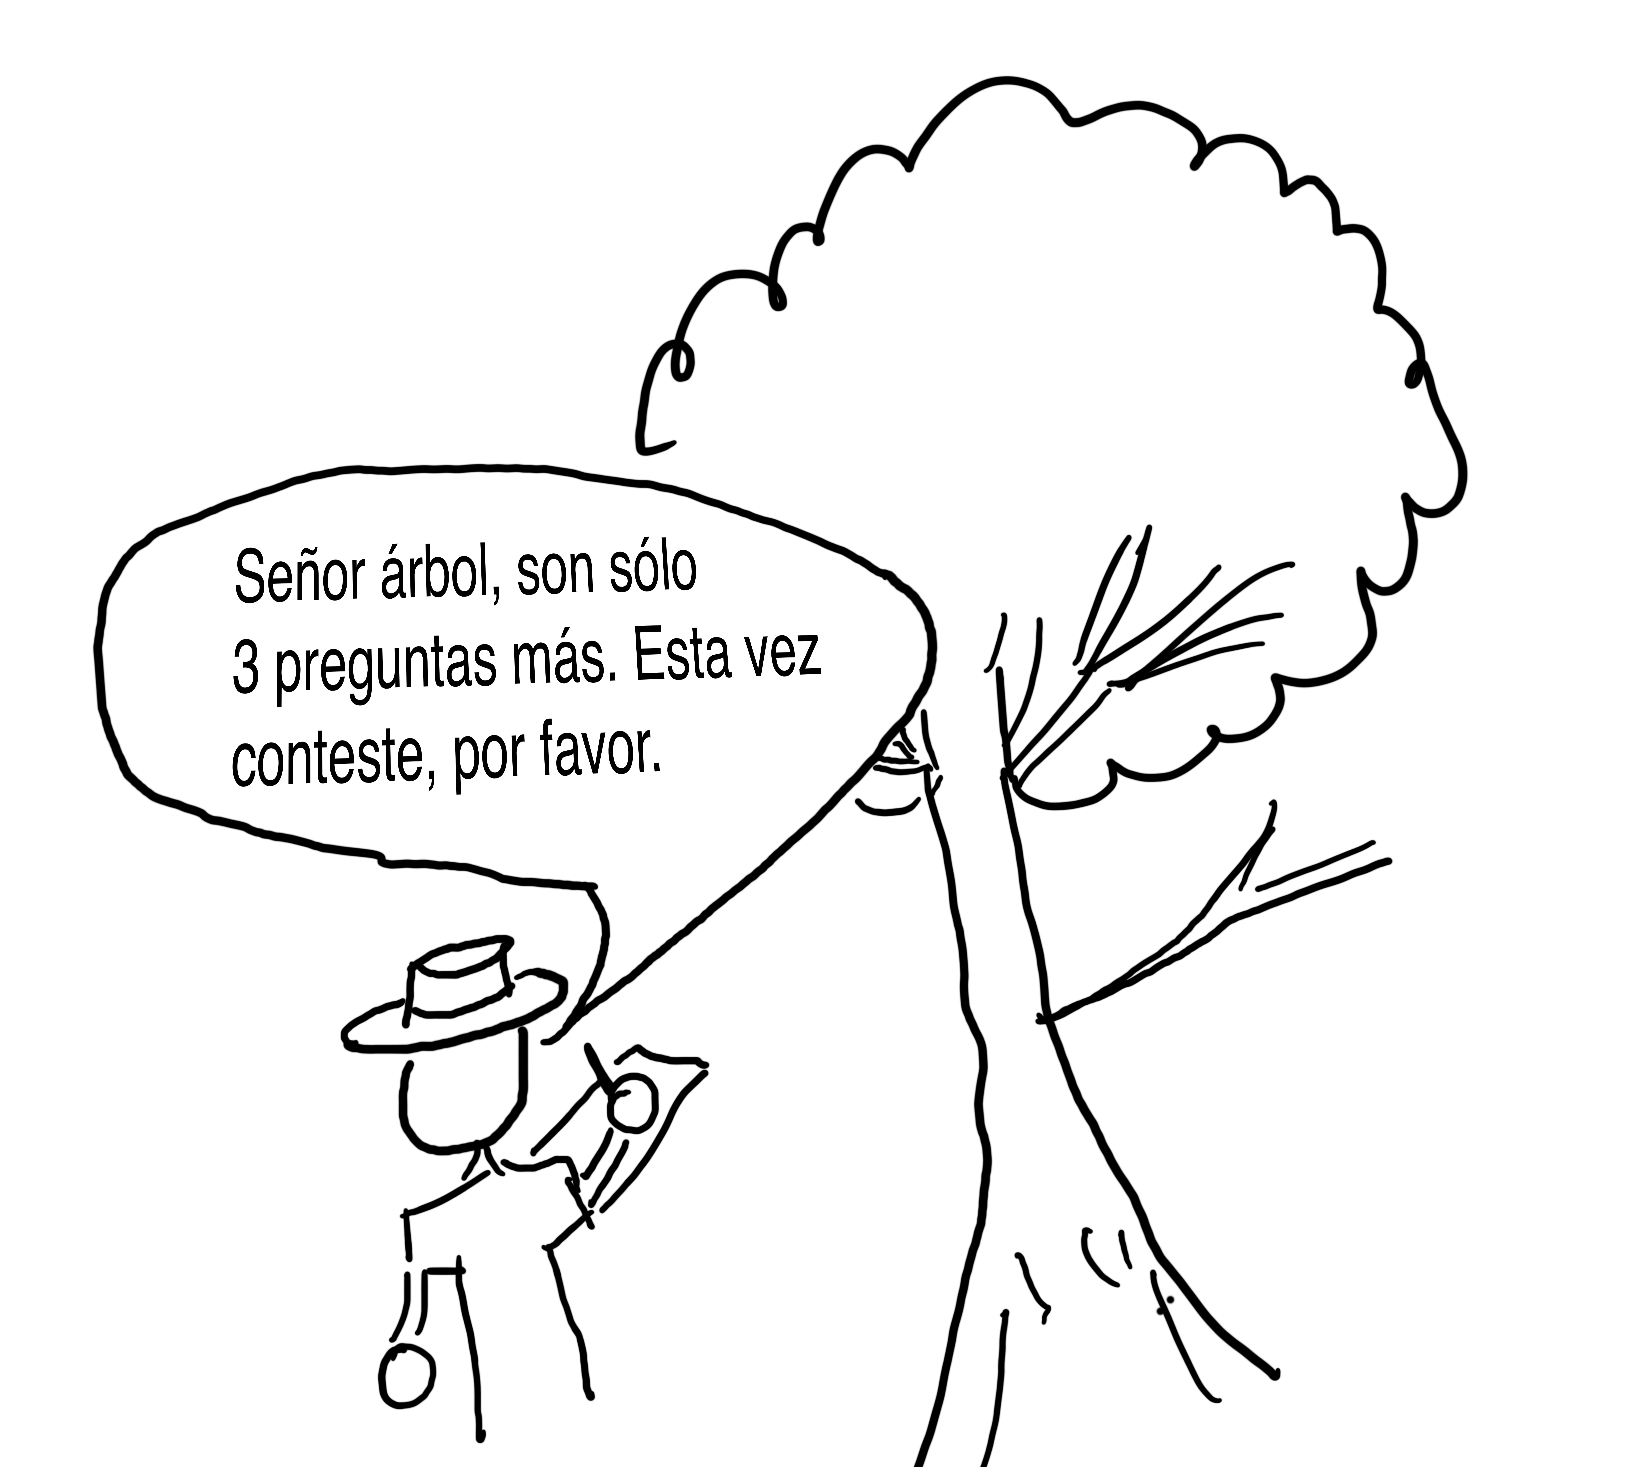
\includegraphics{images/arbol.png}
\caption{No todas las encuestas tienen sentido como cuestionarios}
\end{figure}

\begin{itemize}
\tightlist
\item
  \textbf{Población} Cualquier conjunto no vacío. Algunos ejemplos de poblaciones incluyen: las personas que viven en Guatemala (si me interesa saber algo de los guatemaltecos en general), los árboles del Amazonas (si quiero saber cosas de ecología en torno al río), los perros callejeros en Ciudad de México, los consumidores de una marca de cereal, los coches que transitan por Dubai o los granos de arena en una playa específica de Cancún.
\end{itemize}

\begin{quote}
\textbf{Nota:} Las poblaciones no necesariamente son de seres vivos son sólo conjuntos de cosas que se están estudiando. Las poblaciones usualmente están restringidas al tiempo y al espacio por lo que es importante tener una definición \emph{clara} de quiénes sí están en el estudio, quiénes no y por qué.
\end{quote}

\begin{quote}
\textbf{Nota:} En la mayoría de los problemas de encuestas que enfrentaremos suponemos que la población es de tamaño \emph{finito} \(N\). Esto en contraste con un experimento donde la población es de tamaño infinito.
\end{quote}

\begin{itemize}
\item
  \textbf{Población objetivo} El conjunto de elementos que formarán parte del estudio. Definir la \emph{población objetivo} es complicado en algunas situaciones; por ejemplo, si se desea saber si \emph{los mexicanos} están a favor o en contra de legalizar la marihuana hay que establecer quiénes son \emph{los mexicanos}. ¿Cuentan las personas con nacionalidad mexicana que residen en el extranjero? ¿Cuentan los menores de edad? ¿Qué pasa con los extranjeros que son residentes?
\item
  \textbf{Población muestreada} Es el conjunto de elementos sobre los cuales se tomó la muestra para el análisis estadístico. \emph{Idealmente} la población objetivo y la muestreada deberían de ser igual pero el mundo no es tan bello. En encuestas de consumo, por ejemplo, usualmente no se muestrean zonas remotas o de muy bajos recursos. En encuestas de elecciones si bien la población objetivo son \emph{todas las personas que voten el día de la elección}, como la mayoría se hacen \emph{antes} de la elección (exceptuando las de salida) entonces se aproxima la definición de \emph{votante} buscando incluir sólo aquellos que estén registrados en el padrón electoral o bien aquellos que al ser encuestados digan que \emph{sí} van a votar.
\end{itemize}

\begin{quote}
A veces a la población se le conoce como \emph{el conjunto universo} y es por esto que se denota:
\[
\mathcal{U} = \{ u_1, u_2, \dots \} 
\]
con \(u_i\) siendo sus elementos. Nosotros (hasta que se diga lo contrario) supondremos que la muestreada coincide con la objetivo y por tanto esa \(\mathcal{U}\) será sólo \textbf{la población}.
\end{quote}

\begin{figure}
\centering
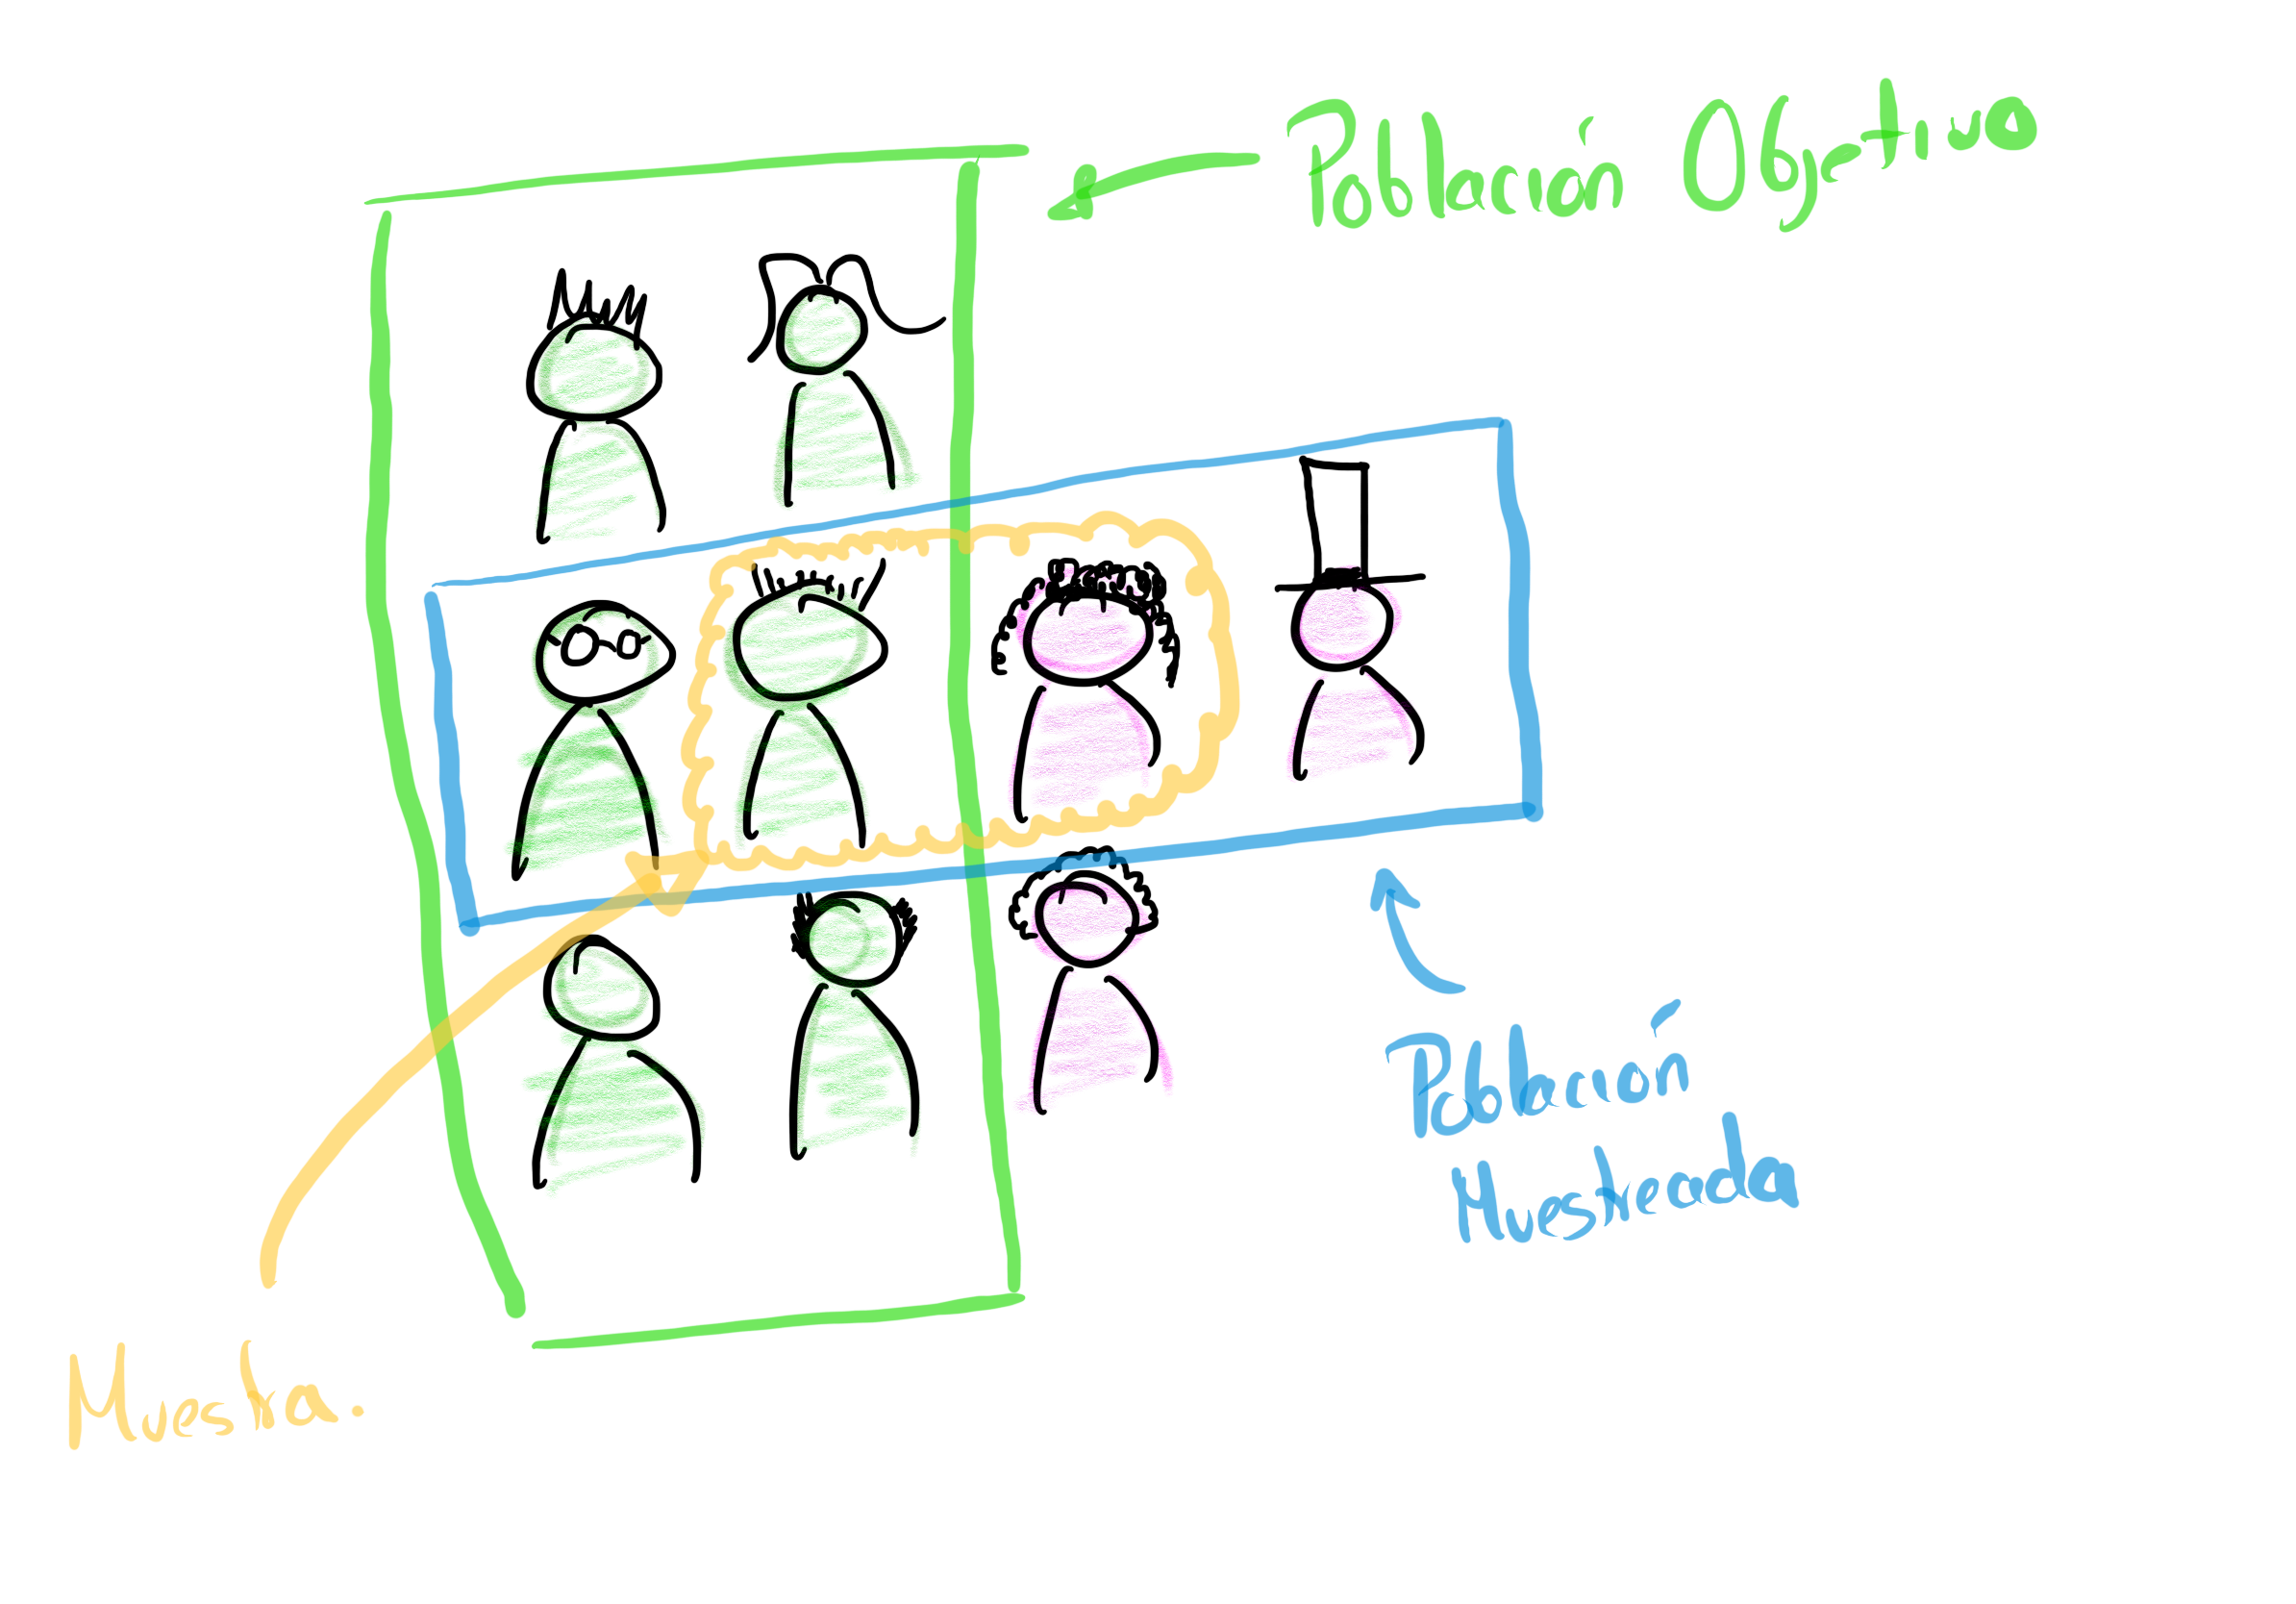
\includegraphics{images/muestra.png}
\caption{Diferencia entre población objetivo, población muestreada y muestra}
\end{figure}

\begin{itemize}
\tightlist
\item
  \textbf{Muestra} Un subconjunto de la población muestreada. Si la muestra coincide con la población muestreada se dice que es un \textbf{censo}. Los ``mejores'' censos (para nosotros) son aquellos donde la población muestreada y la población objetivo coinciden (porque ya medimos todo lo que queríamos). Para el propósito de estas notas los únicos \textbf{censos} que consideraremos son aquellos donde la población muestreada es la objetivo.
\end{itemize}

\begin{quote}
La muestra es un subconjunto de la población:
\[
\mathcal{S} = \{ s_1, s_2, \dots \} \subseteq \mathcal{U}
\]
con \(s_i\) siendo sus elementos. Nosotros sólo consideraremos muestras que son de tamaño finito, \(n\).
\end{quote}

\begin{quote}
\textbf{Nota:} Hasta ahora no estamos hablando de \emph{muestras aleatorias}. Esta definición habla de cualquier subconjunto no necesariamente uno que se haya obtenido por algún mecanismo aleatorio. Por ejemplo, si durante una pandemia se le pide a todas las personas de una población con apellidos de la A a la F acudan a una institución esto sí es una muestra (dado que es subconjunto de la población) pero podría argumentarse no es una muestra aleatoria (pues el proceso de selección fue determinista).
\end{quote}

\begin{quote}
\textbf{Nota} A menos que se especifique lo contrario, el vació, \(\emptyset\) es una muestra.
\end{quote}

\begin{figure}
\centering

\includegraphics{images/muestravacia.jpg}
\caption{Hay que ser muy claros para especificar que queremos una muestra con \(n >0\)}
\end{figure}

\begin{itemize}
\tightlist
\item
  \textbf{Marco muestral} Una lista a partir de la cual se selecciona la muestra para la encuesta. Puede ser, en un salón de clases, la lista completa de alumnos. En estudios de agricultura usualmente la lista son \emph{parcelas de tierra} aunque interese estudiar los cultivos mientras que en poblaciones grandes de personas el marco suele ser una lista de casas (dado que no se sabe qué persona vive dónde) o bien un mapa de calles y colonias. Para el INEGI es común usar las \emph{Áreas Geoestadísticas Básicas} (AGEB) las cuales son divisiones fijas (pequeñísimas, como una manzana) del mapa de México.
\end{itemize}

\begin{figure}
\centering
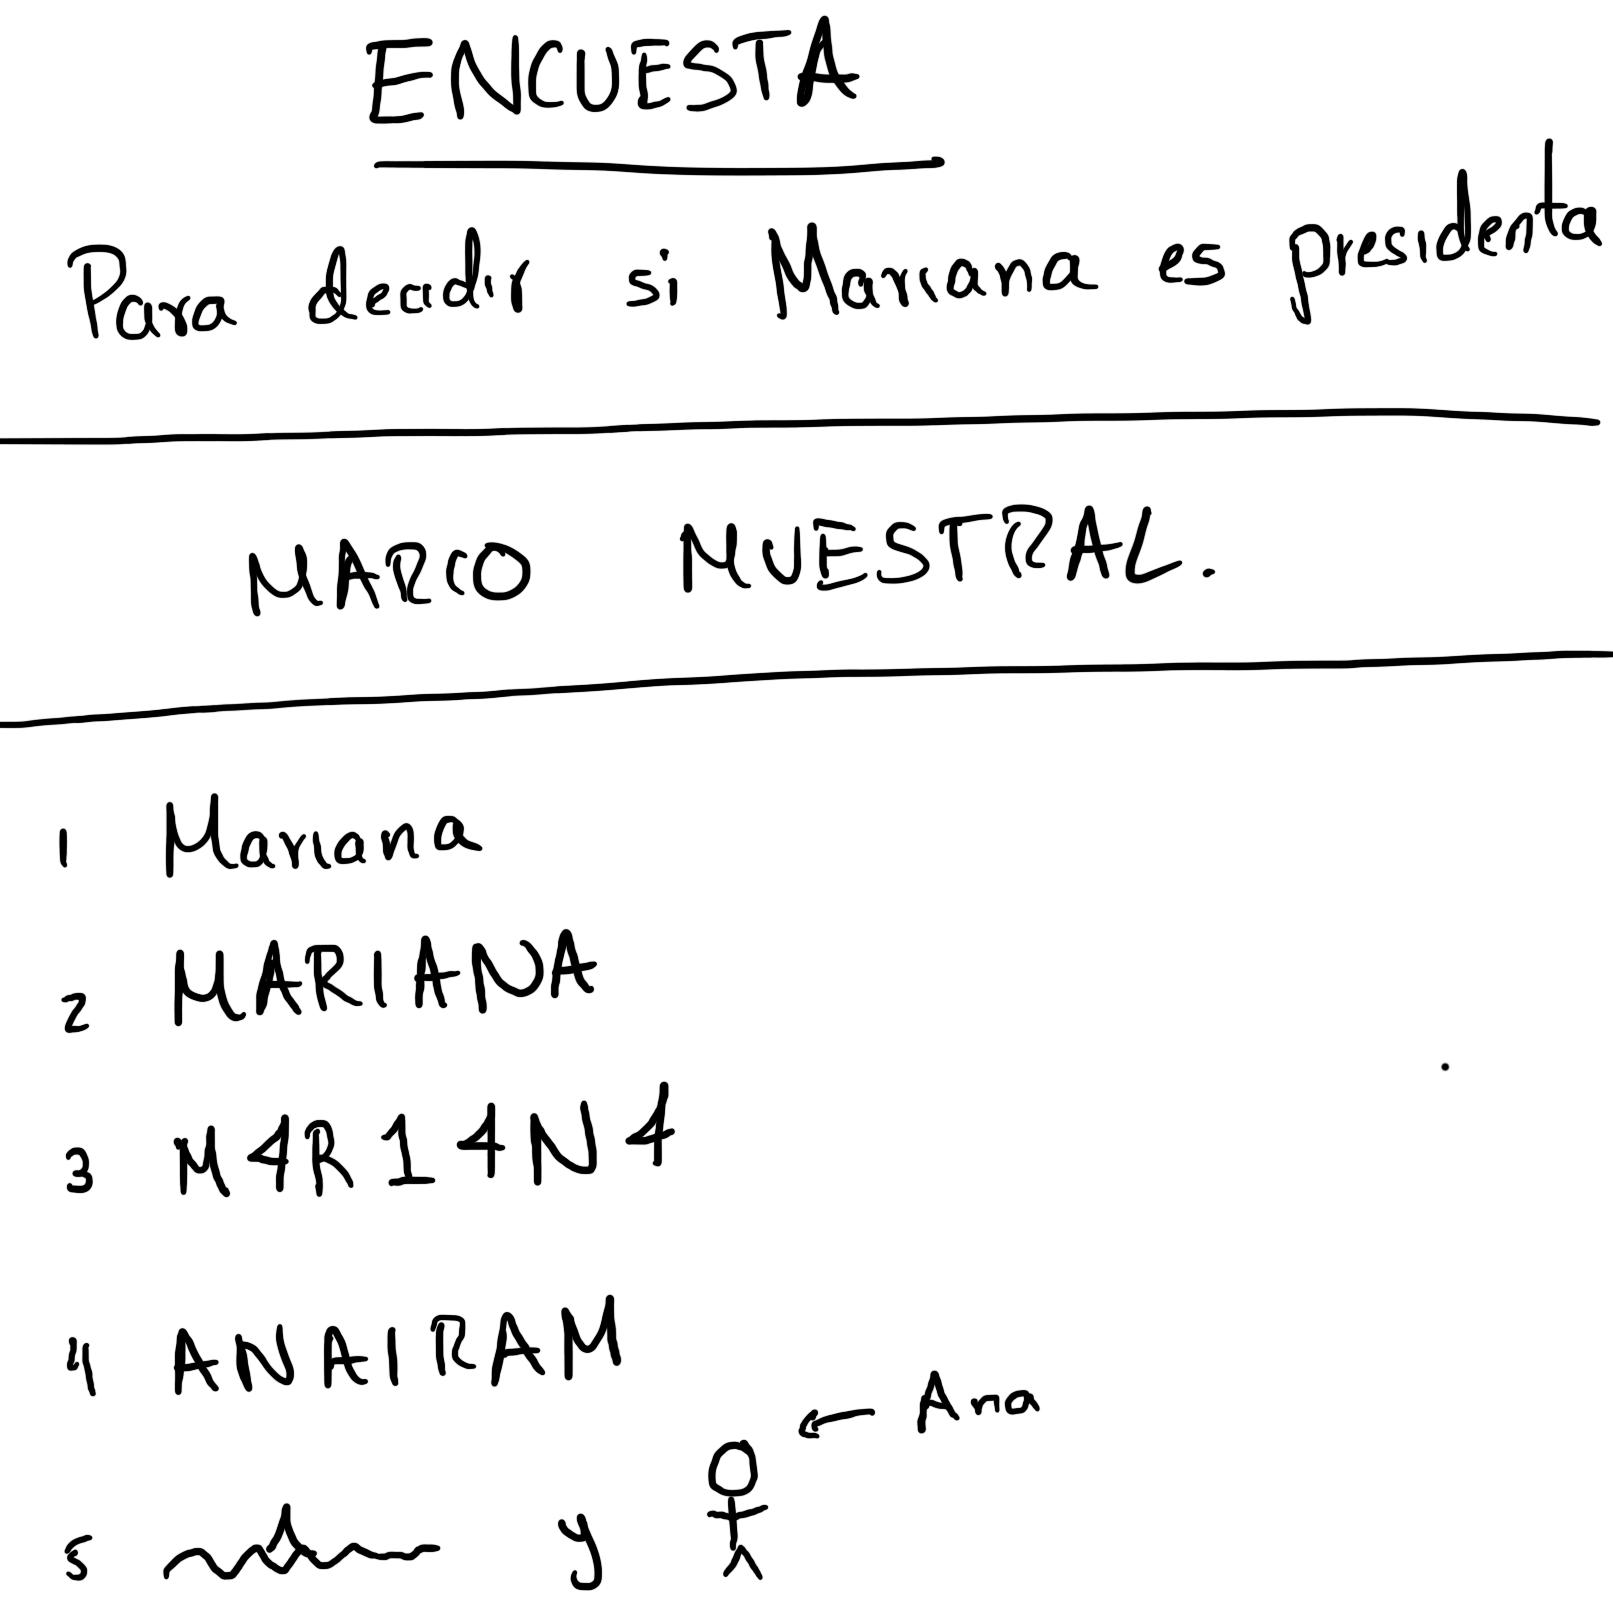
\includegraphics{images/samplingframe.png}
\caption{Este marco muestral está amañado}
\end{figure}

\begin{itemize}
\item
  \textbf{Unidad de muestreo} Una unidad que puede seleccionarse del marco muestral. Por ejemplo, en la lista de casas la \emph{unidad de muestreo} sería una casa. Por otro lado, en una lista de parcelas la \emph{unidad} es la parcela. Si se tiene una lista de estudiantes en un grupo la \emph{unidad} serían los estudiantes. Puede que haya múltiples unidades de muestreo en la misma encuesta por ejemplo, si se desea hacer una encuesta para evaluar alumnos de las escuelas. Suponiendo que el muestreo ocurre de la siguiente forma: 1) primero sólo se tiene la lista de escuelas por lo que se seleccionan al azar un número de escuelas; 2) una vez las investigadoras llegan a la escuela elegida, obtienen la lista de los alumnos inscritos y muestrean sobre ellos. En este escenario hay dos niveles de marcos muestrales (la lista de escuelas de manera inicial y la lista de alumnos por escuela que se obtiene una vez llegas a la escuela elegida). La primera unidad de muestreo (Unidad Primaria de Muestreo) es la escuela; la segunda unidad de muestreo (Unidad Secundaria de Muestreo) son los alumnos.
\item
  \textbf{Unidad de observación} El objeto que interesa medir. En el caso de una encuesta dirigida a personas donde se utiliza una lista de casas para encontrar a las personas, la unidad de muestreo es la casa (el objeto de la lista) pero la unidad de observación son las personas que viven dentro de la casa (lo que quiero medir). Una cosa muy parecida (pero no idéntica) es tener una lista de casas y desear estudiar propiedades de la casa (digamos, tamaño). En ese caso la unidad de muestreo y observación coinciden: son la casa.
\end{itemize}

\hypertarget{anuxe1lisis-exploratorio-de-datos}{%
\chapter{Análisis Exploratorio de Datos}\label{anuxe1lisis-exploratorio-de-datos}}

\hypertarget{inicio}{%
\section{Inicio}\label{inicio}}

Siempre que inicies un nuevo trabajo en \texttt{R} ¡no olvides borrar el historial!

\begin{Shaded}
\begin{Highlighting}[]
\FunctionTok{rm}\NormalTok{(}\AttributeTok{list =} \FunctionTok{ls}\NormalTok{()) }\CommentTok{\#Clear all}
\end{Highlighting}
\end{Shaded}

\hypertarget{libreruxedas}{%
\section{Librerías}\label{libreruxedas}}

Para este análisis vamos a tener que llamar a las siguientes librerías previamente instaladas (por única vez) con \texttt{install.packages}:

\begin{Shaded}
\begin{Highlighting}[]
\FunctionTok{library}\NormalTok{(tidyverse)}
\FunctionTok{library}\NormalTok{(dplyr)}
\FunctionTok{library}\NormalTok{(moments)}
\FunctionTok{library}\NormalTok{(lubridate)}
\FunctionTok{library}\NormalTok{(ggcorrplot)}
\FunctionTok{library}\NormalTok{(ks)}
\end{Highlighting}
\end{Shaded}

Si no tienes una librería puedes instalarla escribiendo en la consola el \texttt{install} junto con su nombre:

\begin{Shaded}
\begin{Highlighting}[]
\FunctionTok{install.packages}\NormalTok{(}\StringTok{"lubridate"}\NormalTok{)}
\end{Highlighting}
\end{Shaded}

\hypertarget{base-a-analizar}{%
\section{Base a analizar}\label{base-a-analizar}}

Como ejemplo analizaremos la base de \emph{Carpetas de Investigación de la Fiscalía General de Justicia} de la CDMX para el año 2018 y mes de Diciembre misma que se encuentra \href{https://datos.cdmx.gob.mx/explore/dataset/carpetas-de-investigacion-pgj-cdmx/download/?format=csv\&refine.ao_hechos=2018\&refine.mes_hechos=Diciembre\&timezone=America/Mexico_City\&lang=es\&use_labels_for_header=true\&csv_separator=\%2C}{en este link}

\begin{quote}
Si el link anterior no abre ve al sitio \url{https://datos.cdmx.gob.mx/explore/dataset/carpetas-de-investigacion-pgj-cdmx/table/?refine.ao_hechos=2018} y elige la opción de año 2018, mes diciembre y descargar como csv.
\end{quote}

La forma más fácil en RStudio es yéndonos a \texttt{Import\ Dataset} en el panel derecho seguido de \texttt{From\ Text} y seleccionamos el archivo. En este caso hay dos opciones cualquiera de las dos opciones funciona: si en tu ordenador no sirve una, ¡prueba la otra!

En mi caso el archivo está en una carpeta que se llama \texttt{datasets} y se lee de la siguiente manera:

\begin{Shaded}
\begin{Highlighting}[]
\NormalTok{datos }\OtherTok{\textless{}{-}} \FunctionTok{read.csv}\NormalTok{(}\StringTok{"datasets/carpetas{-}de{-}investigacion{-}pgj{-}cdmx.csv"}\NormalTok{)}
\end{Highlighting}
\end{Shaded}

\hypertarget{definiciones-y-notaciuxf3n}{%
\section{Definiciones y notación}\label{definiciones-y-notaciuxf3n}}

Siguiendo la definición de \protect\hyperlink{ref-gelman2013bayesian}{Gelman et al.} (\protect\hyperlink{ref-gelman2013bayesian}{2013}) , denotamos el conjunto de datos observados como la matriz (\emph{base de datos}) de \(n \times \ell\)
\[
Z = \begin{pmatrix} 
z_1 \Big| z_2 \Big| \dots \Big| z_{\ell}
\end{pmatrix}
\]
donde \(\ell \in \mathbb{N}\) con \(\ell > 0\) y las \(z_i\) sin pérdida de generalidad, son vectores columna de longitud \(n\) (\(z_i = (z_{i,1}, z_{i,2}, \dots, z_{i,n})^T\)). Una columna \(z_{k}\) con \(0 \leq k \leq \ell\) se le conoce como:

\begin{itemize}
\item
  \emph{Numérica} si \(z_{k} \in \mathbb{R}^{n}\). En particular es entera si \(z_{j} \in \mathbb{Z}^{n}\).
\item
  \emph{Categórica} si cada entrada de \(z_{k}\) es una indicadora de pertenencia a algún conjunto (por ejemplo \texttt{Hombre\ /\ Mujer} ó \texttt{Ingresos\ Altos\ /\ Ingresos\ Medios\ /\ Ingresos\ Bajos}). Usualmente \(z_{k}\) se representa con un caracter o con un entero. Una variable cateórica puede ser \emph{lógica} si \(z_{k}\) es un indicador que toma alguno de los dos valores: TRUE ó FALSE.
\item
  \emph{Ordinal} Una variable ordinal es aquél \(z_{k} \in \mathcal{C}\) donde sobre \(\mathcal{C}\) existe un orden total; es decir si \(x,y,w\in z_{k}\) se tiene que:

  \begin{enumerate}
  \def\labelenumi{\alph{enumi}.}
  \tightlist
  \item
    Ocurre al menos una de las siguientes: \(x \leq y\) ó \(x \geq y\).
  \item
    Si \(x \leq y\) y \(y \geq w\) entonces \(x \leq w\)
  \item
    Si \(x \leq y\) y \(x \geq y\) entonces \(x = y\).
    Variables numéricas univariadas son ordinales por el orden natural de \(\mathbb{R}\).
  \end{enumerate}
\item
  \emph{Caracter} si \(z_{k}\) es un caracter o una cadena de caracteres donde los caracteres son el objeto de análisis en sí (no como pertenencia). Por ejemplo si cada entrada \(z_{k,m}\) representa un Tweet.
\end{itemize}

\textbf{OJO} Los datos \(z_{k,m}\) son variables fijas ya dadas y \textbf{NO SON ALEATORIAS}.

En el caso de nuestra base de datos podemos resumir la información contenida en la misma mediante \texttt{glimpse}:

\begin{Shaded}
\begin{Highlighting}[]
\NormalTok{datos }\SpecialCharTok{\%\textgreater{}\%} \FunctionTok{glimpse}\NormalTok{()}
\end{Highlighting}
\end{Shaded}

\begin{verbatim}
## Rows: 19,861
## Columns: 18
## $ año_hechos           <int> 2018, 2018, 2018, 2018, 2018, 2018, 2018, 2018, 2~
## $ mes_hechos           <chr> "Diciembre", "Diciembre", "Diciembre", "Diciembre~
## $ fecha_hechos         <chr> "2018-12-13 12:00:00", "2018-12-22 19:00:00", "20~
## $ delito               <chr> "USURPACIÓN DE IDENTIDAD", "SUSTRACCION DE MENORE~
## $ categoria_delito     <chr> "DELITO DE BAJO IMPACTO", "DELITO DE BAJO IMPACTO~
## $ fiscalía             <chr> "INVESTIGACIÓN EN MIGUEL HIDALGO", "INVESTIGACIÓN~
## $ agencia              <chr> "MH-2", "59", "BJ-1", "IZP-9", "75TER", "FDS-5", ~
## $ unidad_investigacion <chr> "UI-1SD", "UI-1CD", "UI-1SD", "UI-2SD", "3 S/D", ~
## $ colonia_hechos       <chr> "LOMAS DE SOTELO", NA, "DEL VALLE CENTRO", "AMPLI~
## $ alcaldia_hechos      <chr> "MIGUEL HIDALGO", "CUAUTLA", "BENITO JUAREZ", "IZ~
## $ fecha_inicio         <chr> "2019-06-16 12:14:09", "2019-06-06 16:26:15", "20~
## $ mes_inicio           <chr> "Junio", "Junio", "Febrero", "Febrero", "Abril", ~
## $ ao_inicio            <int> 2019, 2019, 2019, 2019, 2019, 2019, 2019, 2019, 2~
## $ calle_hechos         <chr> "AV. CONSCRIPTO", "AVENIDFA DIEZ DE MARZO", "FELI~
## $ calle_hechos2        <chr> ".", "HECHOS EN CUAUTLA MORELOS", "ESQUINA COYOAC~
## $ longitud             <dbl> -99.22535, NA, -99.17088, -99.03016, -99.13423, -~
## $ latitud              <dbl> 19.44028, NA, 19.37207, 19.34797, 19.54788, 19.34~
## $ Geopoint             <chr> "19.4402832543,-99.2253527208", "", "19.372068287~
\end{verbatim}

Notamos que el vector columna \texttt{año\_hechos} es una variable numérica mientras que \texttt{mes\_hechos} es categórica. No hay variables lógicas en esta base. Una variable caracter es el vector columna \texttt{calle\_hechos} que no denota un conjunto sino una cadena de caracteres (véanse las faltas de ortografía, por ejemplo).

Al ser la tabla de datos una matriz podemos acceder a la entrada en la fila \(j\) y columna \(k\) haciendo:
\[
\textrm{base}[j,k]
\]
por ejemplo:

\begin{Shaded}
\begin{Highlighting}[]
\NormalTok{datos[}\DecValTok{4}\NormalTok{,}\DecValTok{6}\NormalTok{]}
\end{Highlighting}
\end{Shaded}

\begin{verbatim}
## [1] "INVESTIGACIÓN EN IZTAPALAPA"
\end{verbatim}

\begin{quote}
\textbf{NOTACIÓN}
Para facilitar la notación en lo que sigue de estas notas y hasta nuevo aviso, si \(z_k\) es una columna categórica de \(Z\) denotaremos a los elementos de dicha columna como \(C = (c_1, c_2, \dots, c_n) = z_k^T\). Si \(z_k\) es numérica denotamos a los elementos de dicha columna como \(\vec{x} = (x_1, x_2, \dots, x_n) = z_k^T\).
\end{quote}

\hypertarget{estaduxedsticos-univariados}{%
\section{Estadísticos univariados}\label{estaduxedsticos-univariados}}

\hypertarget{definiciuxf3n-estaduxedstico}{%
\subsection{Definición {[}Estadístico{]}}\label{definiciuxf3n-estaduxedstico}}

Un estadístico es una función cuyo dominio es la matriz de datos observados \(Z\) o una columna de la misma. Es decir, un estadístico es cualquier función de los datos (ver \protect\hyperlink{ref-wolfe2017intuitive}{Wolfe and Schneider} (\protect\hyperlink{ref-wolfe2017intuitive}{2017})).

\textbf{A continuación veremos algunos ejemplos de estadísticos así como su interpretación.}

\textbf{1. Media poblacional} Dado un vector de datos numéricos \(\vec{x} = (x_1, x_2, \dots, x_n)^T\) definimos la media poblacional como:
\[
  \bar{x} = \dfrac{1}{n} \sum\limits_{i=1}^{n} x_i, \qquad x_i \in \mathbb{R}
  \]
En el caso de nuestros datos podemos \textbf{calcular el promedio de delitos por día} como sigue. Primero necesitamos especificar a \texttt{R} que la \texttt{fecha\_hechos} es una fecha. Esto lo hacemos mediante la función \texttt{ymd\_hms} (\texttt{year-month-day\_hour-minute-second}) del paquete de \texttt{lubridate} y la función \texttt{mutate} (que cambia una columna de la base de datos). El siguiente código le indica a \texttt{R} que cambie la columna \texttt{fecha\_hechos} volviéndola a leer como fecha:

\begin{Shaded}
\begin{Highlighting}[]
\NormalTok{datos }\OtherTok{\textless{}{-}}\NormalTok{ datos }\SpecialCharTok{\%\textgreater{}\%} \FunctionTok{mutate}\NormalTok{(}\AttributeTok{fecha\_hechos =} \FunctionTok{ymd\_hms}\NormalTok{(fecha\_hechos))}
\end{Highlighting}
\end{Shaded}

Para mantener sólo la fecha y eliminar la hora de \texttt{fecha\_hechos} podemos generar una nueva columna como sigue:

\begin{Shaded}
\begin{Highlighting}[]
\NormalTok{datos }\OtherTok{\textless{}{-}}\NormalTok{ datos }\SpecialCharTok{\%\textgreater{}\%} \FunctionTok{mutate}\NormalTok{(}\AttributeTok{fecha =} \FunctionTok{date}\NormalTok{(fecha\_hechos))}
\end{Highlighting}
\end{Shaded}

Finalmente podemos contar (\texttt{tally}) observaciones agrupadas (\texttt{group\_by}) por día mediante la combinación de ambas funciones:

\begin{Shaded}
\begin{Highlighting}[]
\NormalTok{conteo\_delitos }\OtherTok{\textless{}{-}}\NormalTok{ datos }\SpecialCharTok{\%\textgreater{}\%} \FunctionTok{group\_by}\NormalTok{(fecha) }\SpecialCharTok{\%\textgreater{}\%} \FunctionTok{tally}\NormalTok{()}
\end{Highlighting}
\end{Shaded}

\begin{verbatim}
## # A tibble: 6 x 2
##   fecha          n
##   <date>     <int>
## 1 2018-12-01   674
## 2 2018-12-02   584
## 3 2018-12-03   790
## 4 2018-12-04   640
## 5 2018-12-05   724
## 6 2018-12-06   718
\end{verbatim}

Hay distintas formas de calcular la media. La primera es tomando la columna directo, para acceder a una columna utilizamos el signo de pesos \(\$\) como sigue:
\[
\texttt{base} \texttt{\$} \texttt{columna}
\]

En nuestro caso:

\begin{Shaded}
\begin{Highlighting}[]
\FunctionTok{mean}\NormalTok{(conteo\_delitos}\SpecialCharTok{$}\NormalTok{n)}
\end{Highlighting}
\end{Shaded}

\begin{verbatim}
## [1] 640.6774
\end{verbatim}

O bien podemos usar la función \texttt{summarise} integrada en \texttt{dplyr}:

\begin{Shaded}
\begin{Highlighting}[]
\NormalTok{conteo\_delitos }\SpecialCharTok{\%\textgreater{}\%} \FunctionTok{summarise}\NormalTok{(}\FunctionTok{mean}\NormalTok{(n))}
\end{Highlighting}
\end{Shaded}

\begin{verbatim}
## # A tibble: 1 x 1
##   `mean(n)`
##       <dbl>
## 1      641.
\end{verbatim}

\begin{quote}
\textbf{NOTA} Una media como está descrita arriba no aplica para datos circulares. Por ejemplo, si queremos determinar el mes promedio en el que ocurren las lluvias dentro de los años se sabe que después del mes 12 continúa el mes 1 del próximo año. Una media tradicional no considera datos que pueden ser descritos mediante aritmética modular (como los meses). Para ello se utiliza la media circular:
\end{quote}

\textbf{1.1 Media circular} Consideremos el problema de determinar el día promedio de la semana en que más ocurren delitos (de Lunes a Domingo). Podemos resumir los eventos usando la función \texttt{weekdays}:

\begin{Shaded}
\begin{Highlighting}[]
\NormalTok{datos      }\OtherTok{\textless{}{-}}\NormalTok{ datos }\SpecialCharTok{\%\textgreater{}\%} \FunctionTok{mutate}\NormalTok{(}\StringTok{\textasciigrave{}}\AttributeTok{Día de la Semana}\StringTok{\textasciigrave{}} \OtherTok{=} \FunctionTok{weekdays}\NormalTok{(fecha))}
\NormalTok{conteo.dia }\OtherTok{\textless{}{-}}\NormalTok{ datos }\SpecialCharTok{\%\textgreater{}\%} \FunctionTok{group\_by}\NormalTok{(}\StringTok{\textasciigrave{}}\AttributeTok{Día de la Semana}\StringTok{\textasciigrave{}}\NormalTok{) }\SpecialCharTok{\%\textgreater{}\%} \FunctionTok{count}\NormalTok{()}
\end{Highlighting}
\end{Shaded}

de donde se tiene el conteo:

\begin{tabular}{lr}
\toprule
Día de la Semana & n\\
\midrule
Monday & 3251\\
Saturday & 3197\\
Friday & 2833\\
Sunday & 2722\\
Wednesday & 2701\\
\addlinespace
Thursday & 2679\\
Tuesday & 2478\\
\bottomrule
\end{tabular}

Para obtener el día promedio representamos cada uno de los días en el círculo usando coordenadas polares. Nota que el radio es irrelevante en este caso: sólo el ángulo importa; de ahí que tomemos \(r = 1\):

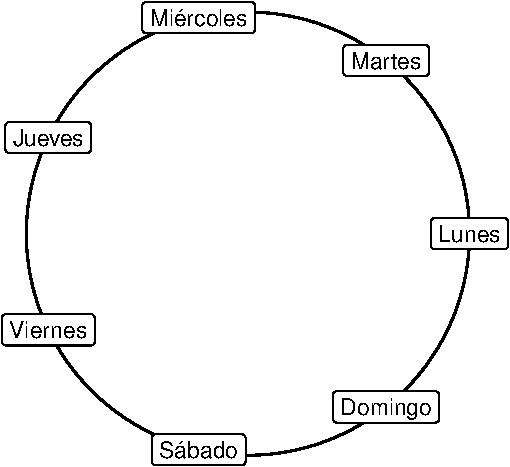
\includegraphics{Introduccion_a_Muestreo_files/figure-latex/unnamed-chunk-17-1.pdf}

Para un conjunto de mediciones con ángulos \((\theta_1, \theta_2, \dots, \theta_n)^T\) el centro de masa asociado a dichas mediciones es el punto \((\bar{c}, \bar{s})\) donde
\[
\bar{c} = \frac{1}{n}\sum\limits_{i = 1}^n \cos (\theta_i) \qquad \text{y} \qquad \bar{s} = \frac{1}{n}\sum\limits_{i = 1}^n \sin (\theta_i)
\]
La dirección media se define como la solución \(\bar{\theta}\) (si \(\bar{r} > 0\)) a:
\[
\bar{c} = \bar{r}\cos\bar{\theta} \qquad \text{ y } \qquad \bar{s} = \bar{r}\sin\bar{\theta}
\]
donde \(\bar{r}\) se conoce como \emph{la longitud resultante promedio} . Si \(\bar{r} = 0\) no existe dirección media. De manera explícita, por geometría tenemos que:
\[
\bar{r} = (\bar{c}^2 + \bar{s}^2)^{1/2}
\]
y que:
\[
\bar{\theta} = \text{atan2}(\bar{s}/\bar{c}) = \begin{cases}
\text{atan}(\bar{s}/\bar{c}) & \text{ si } \bar{c} \geq 0\\
\text{atan}(\bar{s}/\bar{c}) + \pi & \text{ si } \bar{c} < 0\\
\end{cases}
\]
donde el caso \(\bar{c} = 0\) se interpreta como el límite por la derecha (respectivamente por la izquierda) de la arcotangente de acuerdo con el signo de \(\bar{s}\).

Ahora bien, si tomamos
\[
c=\sum\limits_{i = 1}^n \cos (\theta_i) \qquad \text{y} \qquad \bar{s} =\sum\limits_{i = 1}^n \sin (\theta_i)
\]
podemos definir \emph{la longitud resultante} como \(r=(c^2 + s^2)^{\frac{1}{2}}\), entonces, es perfectamente aceptable tomar \emph{la longitud resultante promedio} previamente definida como:
\[
\bar{r}= (\bar{c}^2 + \bar{s}^2)^{1/2} = \frac{r}{n}
\]
\textgreater{}\textbf{NOTA} Muchos son los casos donde las coordenadas polares son más útiles. Sabemos que las coordenadas polares piden la especificación de un ángulo \(\phi\) y una recta de longitud \(r\). Las coordenadas polares pueden ser utilizadas para especificar puntos en cualquier lugar de un plano, no solamente en el círculo unitario. En lugar de las coordenadas cartesianas \((x_i, y_i)\), las coordenadas polares \((\phi_i, r_i)\) especifican dónde se encuentra cada punto en términos de su dirección y distancia con respecto al origen. Así, nos dan la clara ventaja de separar información tanto de distancia como de dirección en el análisis de datos, mientras que las cartesianas confunden aspectos espaciales.

\textbf{1.2 Varianza Angular(Circular)}
\protect\hyperlink{ref-pewsey2013circular}{Pewsey, Neuhäuser, and Ruxton} (\protect\hyperlink{ref-pewsey2013circular}{2013}) define la varianza circular como:
\[
\textrm{Var} = 1 - \bar{r}
\]
donde \(\bar{r} = (\bar{c}^2 + \bar{s}^2)^{1/2}\) es el resolvente explicado anteriormente. Es importante notar que \(\textrm{Var}\) puede tomar valores en \([0,1]\) y su interpretación es similar a la de la varianza de datos lineales, i.e.~``entre más pequeño sea el valor de la varianza circular, más conectrada es la distribución de los datos'' \protect\hyperlink{ref-fisher1995statistical}{Fisher} (\protect\hyperlink{ref-fisher1995statistical}{1995}).

\textbf{1.3 Dirección Mediana Circular}

Denotamos a la \emph{dirección mediana circular} por \(\tilde{\theta}\). Se puede determinar de manera muy similar al caso del cálculo de la mediana para datos lineales. De tal manera que \(\tilde{\theta}\) es cualquier ángulo \(\phi\) tal que la mitad de los datos se encuentra en el arco \([\phi, \phi + \pi ]\) y la mayoría de los puntos están más cerca de \(phi\) que de \(\phi + \pi\) (Mardia y Jupp). Ahora si \(n\) es impar, la mediana es uno de los datos, en caso contrariom la mediana pasa por el punto medio de dos datos adyacentes.

\textbf{1.4 Desviación Estándar Circular}
Al igual que con datos lineales, la desviación estándar está ítimamente relacionada con la varianza, definimos a la \emph{desviación estándar circular} como
\[
v=\big(-2ln(1-V)\big)^{\frac{1}{2}}= \big(-2ln(\bar{r})\big)^{\frac{1}{2}}
\]
Para más información sobre estadística circular puedes consultar \protect\hyperlink{ref-pewsey2013circular}{Pewsey, Neuhäuser, and Ruxton} (\protect\hyperlink{ref-pewsey2013circular}{2013}), \protect\hyperlink{ref-fisher1995statistical}{Fisher} (\protect\hyperlink{ref-fisher1995statistical}{1995}), \protect\hyperlink{ref-mardia2009directional}{Mardia and Jupp} (\protect\hyperlink{ref-mardia2009directional}{2009}).

\hypertarget{ejercicio}{%
\section{Ejercicio}\label{ejercicio}}

Utiliza la función \texttt{atan2} de \texttt{R} junto con \texttt{cos} y \texttt{sin} para seno y coseno para estimar el día promedio en el que ocurren más delitos según la base \texttt{conteo.dia}.

\textbf{2. Total poblacional} (ver \protect\hyperlink{ref-sarndal2003model}{Särndal, Swensson, and Wretman} (\protect\hyperlink{ref-sarndal2003model}{2003})) Dado un vector de datos numéricos \(\vec{x} = (x_1, x_2, \dots, x_n)^T\) definimos el total poblacional como:

\[
t_{\vec{x}} = \sum\limits_{i=1}^{n} x_i, \qquad x_i \in \mathbb{R}
\]
En este caso de las carpetas de investigación el total nos daría todas las carpetas abiertas durante diciembre. Para ello calculamos el total sumando todos los elementos:

\begin{Shaded}
\begin{Highlighting}[]
\FunctionTok{sum}\NormalTok{(conteo\_delitos}\SpecialCharTok{$}\NormalTok{n)}
\end{Highlighting}
\end{Shaded}

\begin{verbatim}
## [1] 19861
\end{verbatim}

O bien (y esto es una de las cosas interesantes de \texttt{tidyverse}) agregándolo a los cálculos previos:

\begin{Shaded}
\begin{Highlighting}[]
\NormalTok{conteo\_delitos }\SpecialCharTok{\%\textgreater{}\%} \FunctionTok{summarise}\NormalTok{(}\FunctionTok{mean}\NormalTok{(n), }\FunctionTok{sum}\NormalTok{(n))}
\end{Highlighting}
\end{Shaded}

\begin{verbatim}
## # A tibble: 1 x 2
##   `mean(n)` `sum(n)`
##       <dbl>    <int>
## 1      641.    19861
\end{verbatim}

\textbf{3. Varianza poblacional (no ajustada)} Dado un vector de datos numéricos \(\vec{x} = (x_1, x_2, \dots, x_n)^T\) definimos la \emph{varianza poblacional} como\footnote{En \protect\hyperlink{ref-panaretos2016statistics}{Panaretos} (\protect\hyperlink{ref-panaretos2016statistics}{2016}) se conoce como \texttt{sample\ variance} pero para nosotros la muestral tendrá un \(n-1\) en el denominador}:
\[
\sigma^2_{\vec{x}} = \dfrac{1}{n} \sum\limits_{i=1}^{n} (x_i - \bar{x})^2, \qquad x_i \in \mathbb{R}
\]
Misma que podemos calcular con el comando \texttt{var} ya sea directamente en la columna:

\begin{Shaded}
\begin{Highlighting}[]
\FunctionTok{var}\NormalTok{(conteo\_delitos}\SpecialCharTok{$}\NormalTok{n)}
\end{Highlighting}
\end{Shaded}

\begin{verbatim}
## [1] 10046.23
\end{verbatim}

O bien a través del \texttt{summarise} integrando con el anterior:

\begin{Shaded}
\begin{Highlighting}[]
\NormalTok{conteo\_delitos }\SpecialCharTok{\%\textgreater{}\%} \FunctionTok{summarise}\NormalTok{(}\FunctionTok{mean}\NormalTok{(n), }\FunctionTok{sum}\NormalTok{(n), }\FunctionTok{var}\NormalTok{(n))}
\end{Highlighting}
\end{Shaded}

\begin{verbatim}
## # A tibble: 1 x 3
##   `mean(n)` `sum(n)` `var(n)`
##       <dbl>    <int>    <dbl>
## 1      641.    19861   10046.
\end{verbatim}

La raíz cuadrada de la varianza se conoce como \textbf{desviación estándar} y se denota como sigue:
\[
\sigma_{\vec{x}} = \sqrt{\sigma^2_{\vec{x}}}
\]

Recuerda que la varianza se interpreta como la distancia cuadrática promedio a la que están los datos. En particular la varianza casi no considera valores que están a menos de \(1\) de distancia de \(\bar{x}\) (pues \((x_i - \bar{x})^2 < 1\) en ese caso) pero le da mayor peso a valores que están muy lejanos (donde \((x_i - \bar{x})^2 \gg 1\) si \(x_i\) está muy lejos de \(\bar{x}\)). Gráficamente:

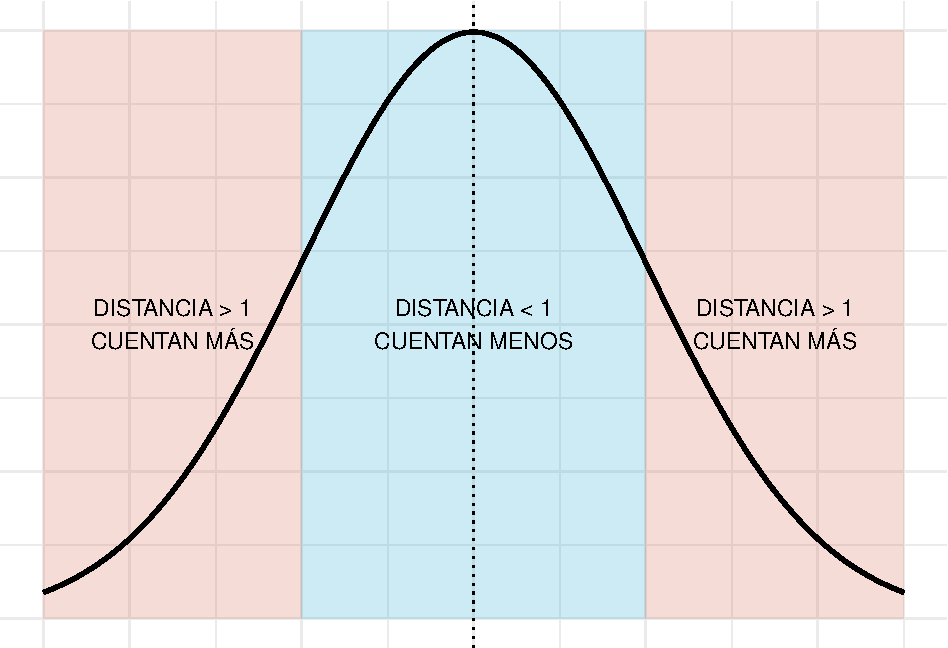
\includegraphics{Introduccion_a_Muestreo_files/figure-latex/unnamed-chunk-22-1.pdf}

Si nos interesara que todos los valores (tanto los cercanos a \(\bar{x}\) como los lejanos) pesaran de manera idéntica entonces usaríamos el MAD:

\textbf{3.1 Varianza angular (circular)} En el caso de datos circulares, \protect\hyperlink{ref-pewsey2013circular}{Pewsey, Neuhäuser, and Ruxton} (\protect\hyperlink{ref-pewsey2013circular}{2013}) define la varianza circular como:
\[
\textrm{Var} = 1 - \bar{r}
\]
donde \(\bar{r} = (\bar{c}^2 + \bar{s}^2)^{1/2}\) es el resolvente explicado anteriormente.

\textbf{4. Desviación Media Absoluta (MAD)} Dado un vector de datos numéricos \(\vec{x} = (x_1, x_2, \dots, x_n)^T\) definimos la desviación media absoluta, MAD, como (\protect\hyperlink{ref-panaretos2016statistics}{Panaretos} (\protect\hyperlink{ref-panaretos2016statistics}{2016})):
\[
\text{MAD}_{\vec{x}} = \frac{1}{n} \sum\limits_{i=1}^{n} | x_i - \bar{x} |
\]

Misma que se puede calcular en \texttt{R} como:

\begin{Shaded}
\begin{Highlighting}[]
\FunctionTok{mad}\NormalTok{(conteo\_delitos}\SpecialCharTok{$}\NormalTok{n, }\AttributeTok{center =} \FunctionTok{mean}\NormalTok{(conteo\_delitos}\SpecialCharTok{$}\NormalTok{n))}
\end{Highlighting}
\end{Shaded}

\begin{verbatim}
## [1] 114.6385
\end{verbatim}

o bien dentro del \texttt{summarise}:

\begin{Shaded}
\begin{Highlighting}[]
\NormalTok{conteo\_delitos }\SpecialCharTok{\%\textgreater{}\%} \FunctionTok{summarise}\NormalTok{(}\FunctionTok{mean}\NormalTok{(n), }\FunctionTok{sum}\NormalTok{(n), }\FunctionTok{var}\NormalTok{(n), }
                             \FunctionTok{mad}\NormalTok{(n, }\AttributeTok{center =} \FunctionTok{mean}\NormalTok{(n)))}
\end{Highlighting}
\end{Shaded}

\begin{verbatim}
## # A tibble: 1 x 4
##   `mean(n)` `sum(n)` `var(n)` `mad(n, center = mean(n))`
##       <dbl>    <int>    <dbl>                      <dbl>
## 1      641.    19861   10046.                       115.
\end{verbatim}

La MAD también es una forma de medir distancia pero en este caso se tiene que todos aportan por igual los muy alejados y los que no:

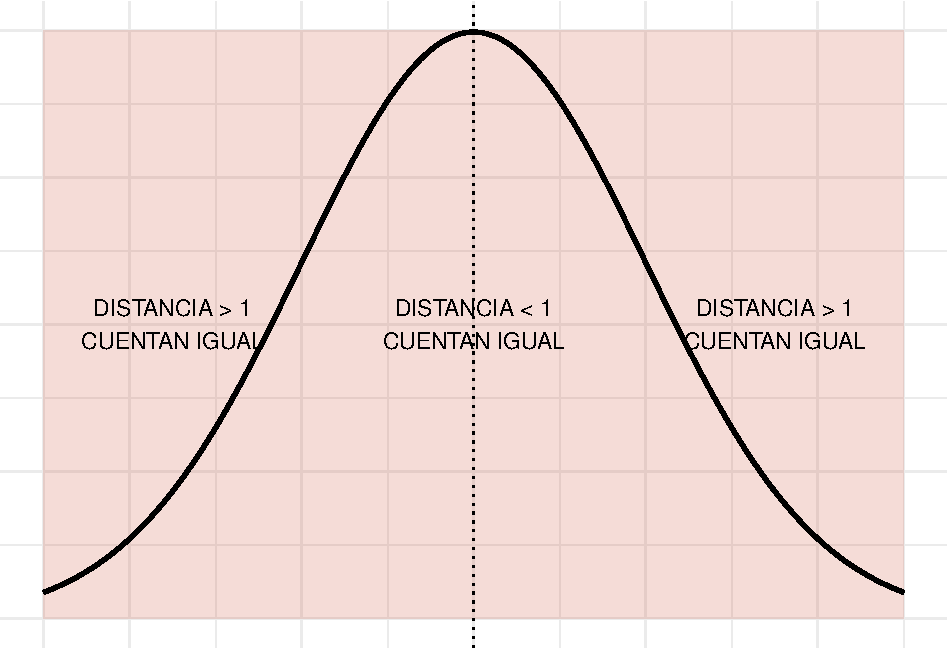
\includegraphics{Introduccion_a_Muestreo_files/figure-latex/unnamed-chunk-25-1.pdf}

\begin{quote}
\emph{Para pensarle}: En el caso de una variable que se supone que es uniforme y no interesa penalizar valores lejanos de la media ¿cuál sería una mejor manera de cuantificar la dispersión MAD ó varianza? ¿en qué casos importaría la otra?
\end{quote}

Las siguientes dos definiciones son con base en conceptos de proba. ¿Los recuerdas?

\textbf{5. Coeficiente de asimetría} Dado un vector de datos numéricos \(\vec{x} = (x_1, x_2, \dots, x_n)^T\) definimos el coeficiente de asimetría de Fisher (\emph{skewness}) como:
\[
\text{Skewness}_{\vec{x}} = \frac{1}{n \sigma^3_{\vec{x}} } \sum\limits_{i = 1}^{n} (x_i - \bar{x})^3
\]

Para más referencias ver \protect\hyperlink{ref-panaretos2016statistics}{Panaretos} (\protect\hyperlink{ref-panaretos2016statistics}{2016}). A fin de interpretar el coeficiente de asimetría podemos dividir esa suma en dos pedazos (olvidándonos de la constante):
\[
\sum\limits_{i = 1}^{n} (x_i - \bar{x})^3 = \underbrace{\sum\limits_{\substack{i = 1 \\ \\ x_i > \bar{x}}}^{n} (x_i - \bar{x})^3}_{\text{A}} + \underbrace{\sum\limits_{\substack{i = 1 \\ \\ x_i < \bar{x}}}^{n} (x_i - \bar{x})^3}_{\text{B}} 
\]
Notamos que si \(|A| > |B|\) la mayor parte de las \(x_i\) (o las que se alejan más de la media) son mayores a \(\bar{x}\) y por tanto los datos van a estar \emph{sesgados a la derecha}:. Por otro lado si \(|B| > |A|\) significa que hay más \(x_i\) (o con mayor peso) del lado izquierdo de la media que del lado derecho de la misma y por tanto los datos están \emph{sesgados a la izquierda}. Datos \emph{insesgados} son aquellos donde \(\text{Skewness}_{\vec{x}} = 0\).

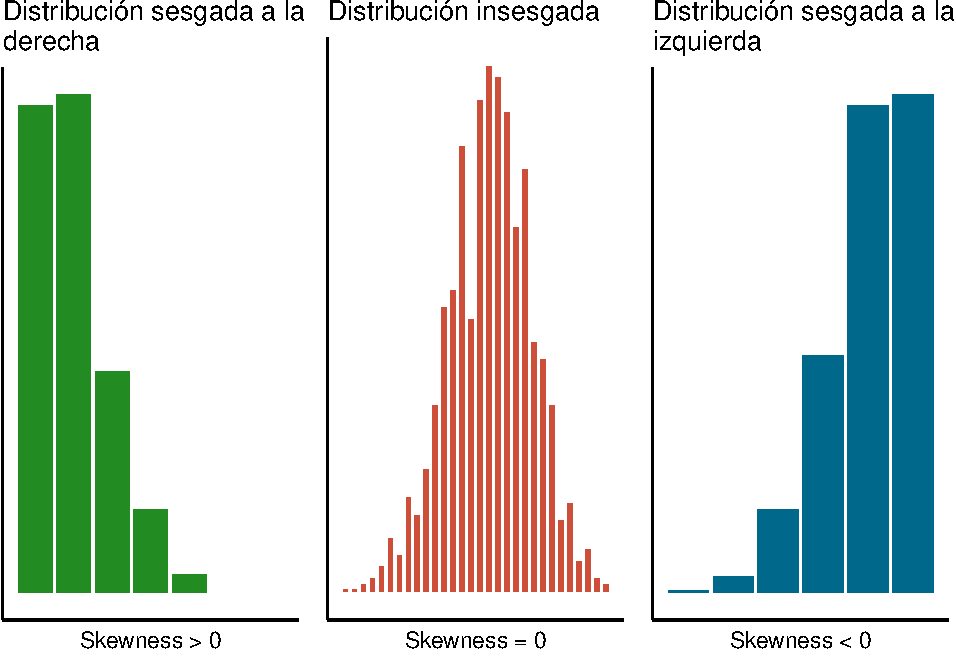
\includegraphics{Introduccion_a_Muestreo_files/figure-latex/unnamed-chunk-26-1.pdf}
En el caso de las carpetas podemos calcular la asimetría que no se encuentra preprogramada en R como sigue:

\begin{Shaded}
\begin{Highlighting}[]
\CommentTok{\#Estimación de la desviación estándar}
\NormalTok{desv.est }\OtherTok{\textless{}{-}} \FunctionTok{sd}\NormalTok{(conteo\_delitos}\SpecialCharTok{$}\NormalTok{n)}

\CommentTok{\#Estimación del x barra}
\NormalTok{x.barra }\OtherTok{\textless{}{-}} \FunctionTok{mean}\NormalTok{(conteo\_delitos}\SpecialCharTok{$}\NormalTok{n)}

\CommentTok{\#Obtención de la n (longitud del vector)}
\NormalTok{n.longitud }\OtherTok{\textless{}{-}} \FunctionTok{length}\NormalTok{(conteo\_delitos}\SpecialCharTok{$}\NormalTok{n)}

\CommentTok{\#Cálculo de la asimetría}
\NormalTok{(}\DecValTok{1}\SpecialCharTok{/}\NormalTok{desv.est}\SpecialCharTok{\^{}}\DecValTok{3}\NormalTok{)}\SpecialCharTok{*}\FunctionTok{mean}\NormalTok{((conteo\_delitos}\SpecialCharTok{$}\NormalTok{n }\SpecialCharTok{{-}}\NormalTok{ x.barra)}\SpecialCharTok{\^{}}\DecValTok{3}\NormalTok{)}
\end{Highlighting}
\end{Shaded}

\begin{verbatim}
## [1] -0.4528209
\end{verbatim}

\begin{quote}
¿Qué implica el resultado anterior?
\end{quote}

\textbf{6. Curtosis} Dado el mismo vector \(\vec{x}\) que en el enunciado anterior el coeficiente de curtosis se define como

\[
\text{Curtosis}_{\vec{x}} = \frac{1}{n \sigma^4_{\vec{x}} } \sum\limits_{i = 1}^{n} (x_i - \bar{x})^4
\]

La interpretación de la curtosis es similar a la que hicimos de la varianza en el sentido que el elevar a la cuarta va a magnificar los efectos de aquellos valores que estén a más de \(\sigma\) de distancia de la media pues podemos reescribir la suma como:

\[
\frac{1}{n \sigma^4_{\vec{x}} } \sum\limits_{i = 1}^{n} (x_i - \bar{x})^4  = \frac{1}{n \sigma^4_{\vec{x}} }  \underbrace{\sum\limits_{\substack{i = 1 \\ \\ | x_i - \bar{x}| < \sigma}}^{n} (x_i - \bar{x})^4}_{\text{A}} + \frac{1}{n \sigma^4_{\vec{x}} }  \underbrace{\sum\limits_{\substack{i = 1 \\ \\ | x_i - \bar{x}| > \sigma}}^{n} (x_i - \bar{x})^4}_{\text{B}} 
\]
Notamos que la única parte importante que apota a la curtosis es la dada por \textbf{B} que es la que capta las \emph{colas} de la distribución (pues ese lado es \(\gg 1\)) . De ahí que podamos decir que, entre dos vectores de datos, uno tiene colas más pesadas que el otro si su curtosis es mayor. En este caso podemos analizar la \texttt{latitud} y \texttt{longitud} de los datos a través de la curtosis:

\begin{Shaded}
\begin{Highlighting}[]
\NormalTok{datos }\SpecialCharTok{\%\textgreater{}\%} \FunctionTok{summarise}\NormalTok{(}\FunctionTok{kurtosis}\NormalTok{(latitud, }\AttributeTok{na.rm =}\NormalTok{ T), }\FunctionTok{kurtosis}\NormalTok{(longitud, }\AttributeTok{na.rm =}\NormalTok{ T))}
\end{Highlighting}
\end{Shaded}

\begin{verbatim}
##   kurtosis(latitud, na.rm = T) kurtosis(longitud, na.rm = T)
## 1                     2.857934                      3.045037
\end{verbatim}

donde se agregó el comando \texttt{na.rm\ =\ T} para eliminar los valores de no respuesta (missing) marcados como \texttt{NA}. Del análisis notamos que la longitud tiene colas más pesadas que la latitud.

\begin{quote}
\textbf{NOTACIÓN} Dado un vector \(\vec{x} = (x_1, x_2, \dots, x_n)^T\) de valores numéricos denotamos el \(j\)-ésimo valor muestral (\(1 \leq j \leq n\)) como \(x_{(j)}\) tal que \(x_{(1)} = \min \{ x_1, x_2, \dots, x_n \}\) y
\[
x_{(j)} = \min \{ x_1, x_2, \dots, x_n \} \setminus \{ x_{(1)}, x_{(2)}, \dots, x_{(j-1)} \}
\]
Es decir \(x_{(j)}\) es el valor en orden \(j\) al momento de ordenar la muestra. Como nota adicional se define \(x_{(0)} = 0\) y \(x_{(n+1)} = 0\).
\end{quote}

\begin{quote}
\textbf{Nota} La curtosis a veces se define con un denominador distinto (en términos de las \(n\)) como en \protect\hyperlink{ref-myatt2007making}{Myatt and Johnson} (\protect\hyperlink{ref-myatt2007making}{2007}).
\end{quote}

\textbf{7. Mediana} Dado un vector de valores numéricos \(\vec{x} = (x_1, x_2, \dots, x_n)^T\) definimos la mediana como (\protect\hyperlink{ref-panaretos2016statistics}{Panaretos} (\protect\hyperlink{ref-panaretos2016statistics}{2016})):
\[
\text{Mediana}_{\vec{x}} = \dfrac{x_{(\lfloor \frac{n+1}{2} \rfloor)} + x_{(\lceil \frac{n+1}{2} \rceil)}}{2} 
\]
La mediana puede calcularse fácilmente haciendo:

\begin{Shaded}
\begin{Highlighting}[]
\FunctionTok{median}\NormalTok{(conteo\_delitos}\SpecialCharTok{$}\NormalTok{n)}
\end{Highlighting}
\end{Shaded}

\begin{verbatim}
## [1] 646
\end{verbatim}

\textbf{8. Cuantil} Dado un vector de valores numéricos \(\vec{x} = (x_1, x_2, \dots, x_n)^T\) el \(\alpha\)-ésimo cuantil está dado por:
\[
\text{Cuantil}_{\vec{x}}(\alpha) = \dfrac{x_{(\lfloor \alpha\cdot (n+1) \rfloor)} + x_{(\lceil \alpha\cdot (n+1)\rceil)}}{2} 
\]
donde \(x_{(0)} = x_{(n+1)} = 0\). \texttt{R} no calcula los cuantiles de manera exacta sino que por velocidad los aproxima mediante la función \texttt{quantile}. Por ejemplo en el cálculo de los cuantiles \(\alpha = 0.1\) y \(\alpha = 0.66\):

\begin{Shaded}
\begin{Highlighting}[]
\NormalTok{conteo\_delitos }\SpecialCharTok{\%\textgreater{}\%} \FunctionTok{summarise}\NormalTok{(}\FunctionTok{quantile}\NormalTok{(n, }\FunctionTok{c}\NormalTok{(}\FloatTok{0.1}\NormalTok{, }\FloatTok{0.66}\NormalTok{)))}
\end{Highlighting}
\end{Shaded}

\begin{verbatim}
## # A tibble: 2 x 1
##   `quantile(n, c(0.1, 0.66))`
##                         <dbl>
## 1                         501
## 2                         707
\end{verbatim}

La función \texttt{summary} también es bastante útil resumiendo múltiples observaciones de la base:

\begin{Shaded}
\begin{Highlighting}[]
\FunctionTok{summary}\NormalTok{(conteo\_delitos}\SpecialCharTok{$}\NormalTok{n)}
\end{Highlighting}
\end{Shaded}

\begin{verbatim}
##    Min. 1st Qu.  Median    Mean 3rd Qu.    Max. 
##   397.0   568.0   646.0   640.7   721.0   790.0
\end{verbatim}

Ésta incluye los \textbf{cuartiles} los cuales corresponden a los cuantiles asociados a \(\alpha =0.25, 0.5, 0.75\) y \(1\).

\begin{quote}
\textbf{Nota} Hay múltiples definiciones de cuantil (ver \protect\hyperlink{ref-hyndman1996sample}{Hyndman and Fan} (\protect\hyperlink{ref-hyndman1996sample}{1996}) para un intento de homologación). En particular \texttt{R} utiliza una distinta y tus cómputos no van a coincidir si lo haces con esta definición y con la de \texttt{R}. Si quieres saber más de \texttt{R} consulta \texttt{?quantile}
\end{quote}

\textbf{9. Rango intercuartílico} Definimos el rango intercuartílico (\protect\hyperlink{ref-panaretos2016statistics}{Panaretos} (\protect\hyperlink{ref-panaretos2016statistics}{2016})) para valores numèricos \(\vec{x} = (x_1, x_2, \dots, x_n)^T\) como la distancia entre el cuantil \(0.75\) y el \(0.25\) (primer y tercer cuartil):
\[
\text{IQR}_{\vec{x}} = \text{Cuantil}_{\vec{x}}(0.75) -  \text{Cuantil}_{\vec{x}}(0.25)
\]

\begin{Shaded}
\begin{Highlighting}[]
\FunctionTok{IQR}\NormalTok{(conteo\_delitos}\SpecialCharTok{$}\NormalTok{n)}
\end{Highlighting}
\end{Shaded}

\begin{verbatim}
## [1] 153
\end{verbatim}

\textbf{10. Valores atípicos (outliers)} Dado un vector de datos numéricos \(\vec{x} = (x_1, x_2, \dots, x_n)^T\) seguimos a \protect\hyperlink{ref-panaretos2016statistics}{Panaretos} (\protect\hyperlink{ref-panaretos2016statistics}{2016}) para definir los valores atípicos \emph{outliers} como aquellas observaciones:
\[
\textrm{Outliers}_{\vec{x}} = \Big\{ x_i \in \vec{x} \big| x_i \not\in \big[ \text{Cuantil}_{\vec{x}}(0.25) - \frac{3}{2} \text{IQR}_{\vec{x}}, \text{Cuantil}_{\vec{x}}(0.75) + \frac{3}{2} \text{IQR}_{\vec{x}}\big] \Big\}
\]
Los \emph{outliers} en esta definción son valores que serían verdaderamente improbables bajo una distribución normal.

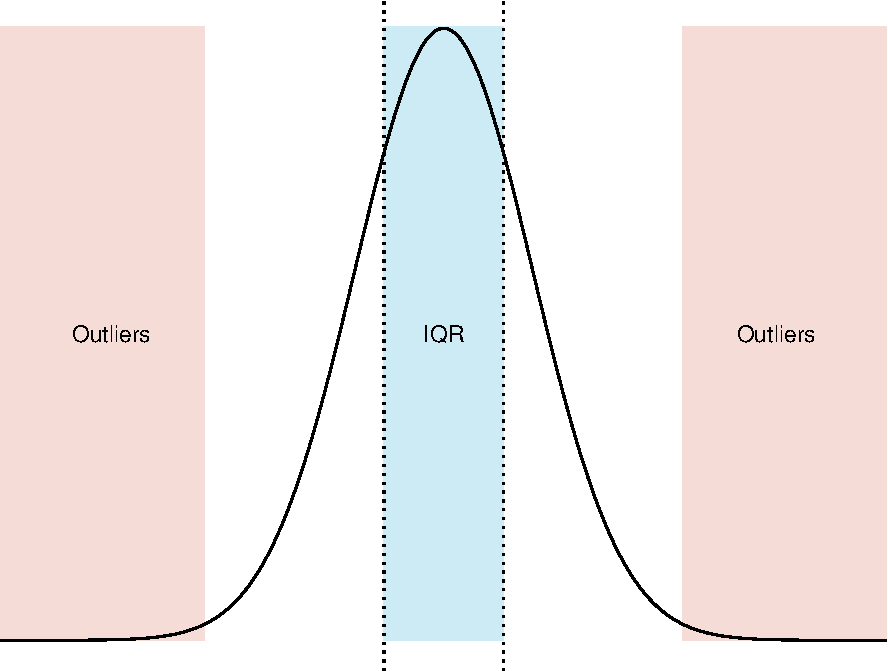
\includegraphics{Introduccion_a_Muestreo_files/figure-latex/unnamed-chunk-33-1.pdf}

Particularmente en el caso de la normal los \emph{outliers} son valores que tienen una probabilidad de salir aproximadamente de 0.0069766 (por eso son atípicos porque no se esperaría que aparecieran nunca).

Para identificar los \emph{outliers} calculamos el IQR primero y los cuartiles:

\begin{Shaded}
\begin{Highlighting}[]
\NormalTok{iqr      }\OtherTok{\textless{}{-}} \FunctionTok{IQR}\NormalTok{(conteo\_delitos}\SpecialCharTok{$}\NormalTok{n)}
\NormalTok{cuartil1 }\OtherTok{\textless{}{-}} \FunctionTok{quantile}\NormalTok{(conteo\_delitos}\SpecialCharTok{$}\NormalTok{n, }\FloatTok{0.25}\NormalTok{)}
\NormalTok{cuartil3 }\OtherTok{\textless{}{-}} \FunctionTok{quantile}\NormalTok{(conteo\_delitos}\SpecialCharTok{$}\NormalTok{n, }\FloatTok{0.75}\NormalTok{)}
\end{Highlighting}
\end{Shaded}

después identificamos el límite inferior y superior del conjunto

\begin{Shaded}
\begin{Highlighting}[]
\NormalTok{lim.inf  }\OtherTok{\textless{}{-}}\NormalTok{ cuartil1 }\SpecialCharTok{{-}} \DecValTok{3}\SpecialCharTok{/}\DecValTok{2}\SpecialCharTok{*}\NormalTok{iqr}
\NormalTok{lim.sup  }\OtherTok{\textless{}{-}}\NormalTok{ cuartil3 }\SpecialCharTok{+} \DecValTok{3}\SpecialCharTok{/}\DecValTok{2}\SpecialCharTok{*}\NormalTok{iqr}
\end{Highlighting}
\end{Shaded}

finalmente preguntamos por cuáles están antes o después:

\begin{Shaded}
\begin{Highlighting}[]
\NormalTok{outliers }\OtherTok{\textless{}{-}}\NormalTok{ conteo\_delitos }\SpecialCharTok{\%\textgreater{}\%} \FunctionTok{filter}\NormalTok{(n }\SpecialCharTok{\textless{}}\NormalTok{ lim.inf }\SpecialCharTok{|}\NormalTok{ n }\SpecialCharTok{\textgreater{}}\NormalTok{ lim.sup)}
\end{Highlighting}
\end{Shaded}

En este caso no tenemos \emph{outliers}.

\begin{quote}
\textbf{NOTA} Según la aplicación que tenemos la definición de \emph{outlier} cambia. La actual es la que se utiliza para datos que pudieran ser descritos mediante una Normal; empero, no siempre esta definición de \emph{outlier} es un buen modelo (por ejemplo en datos como ingreso que son cantidades positivas, con mucha asimetría y cola pesada). Un buen tratamiento sobre los \emph{outliers} puedes encontrarlo en \protect\hyperlink{ref-suri2019outlier}{SURI, Murty, and Athithan} (\protect\hyperlink{ref-suri2019outlier}{2019}).
\end{quote}

\textbf{11. Rango} El rango (\protect\hyperlink{ref-peck2015introduction}{Peck, Olsen, and Devore} (\protect\hyperlink{ref-peck2015introduction}{2015})) se define como la diferencia entre el mínimo y el máximo de los valores de un vector numérico \(\vec{x} = (x_1, x_2, \dots, x_n)^T\):

\[
\textrm{Rango}_{\vec{x}} = \max \{x_1, x_2, \dots, x_n\} - \min \{x_1, x_2, \dots, x_n\}
\]
En \texttt{R} puede calcularse con la resta:

\begin{Shaded}
\begin{Highlighting}[]
\CommentTok{\#Obtenemos máximo y mínimo}
\NormalTok{maximo }\OtherTok{\textless{}{-}} \FunctionTok{max}\NormalTok{(conteo\_delitos}\SpecialCharTok{$}\NormalTok{n)}
\NormalTok{minimo }\OtherTok{\textless{}{-}} \FunctionTok{min}\NormalTok{(conteo\_delitos}\SpecialCharTok{$}\NormalTok{n)}

\CommentTok{\#Rango}
\NormalTok{maximo }\SpecialCharTok{{-}}\NormalTok{ minimo}
\end{Highlighting}
\end{Shaded}

\begin{verbatim}
## [1] 393
\end{verbatim}

\begin{quote}
\textbf{Nota} En algunos casos el rango se refiere al intervalo \([a,b]\) de valores donde \(a = \min \{x_1, x_2, \dots, x_n\}\) y \(b = \max \{x_1, x_2, \dots, x_n\}\). Éste es el caso de la función \texttt{range} en \texttt{R}:
\end{quote}

\begin{Shaded}
\begin{Highlighting}[]
\FunctionTok{range}\NormalTok{(conteo\_delitos}\SpecialCharTok{$}\NormalTok{n)}
\end{Highlighting}
\end{Shaded}

\begin{verbatim}
## [1] 397 790
\end{verbatim}

\textbf{12. Conteo asociado a un conjunto} Sea \(\vec{y} = (y_1, y_2, \dots, y_n)^T\) un vector de datos de cualquier tipo (numéricos, categóricos, lógicos, caracteres, etc). Para un conjunto \(A\) definimos el conteo asociado al conjunto \(A\) como:
\[
\text{Conteo}_{\vec{y}}(A) = \sum\limits_{i = 1}^{n} \mathbb{I}_A (y_i)
\]
donde
\[
\mathbb{I}_A (y) = \begin{cases}
1 & \text{ si } y \in A, \\
0 & \text{ en otro caso },
\end{cases}
\]
es una variable indicadora.

Una forma rápida de obtener dicho conteo en \texttt{R} es mediante \texttt{table}:

\begin{Shaded}
\begin{Highlighting}[]
\FunctionTok{table}\NormalTok{(datos}\SpecialCharTok{$}\NormalTok{delito)}
\end{Highlighting}
\end{Shaded}

\begin{verbatim}
## 
## ABANDONO DE PERSONA              ABORTO  ABUSO DE AUTORIDAD  ABUSO DE CONFIANZA 
##                  53                  15                 102                 276 
##        ABUSO SEXUAL        ACOSO SEXUAL 
##                 252                  30
\end{verbatim}

O bien si se desean contar en la base de datos por ejemplo los delitos de \texttt{ABANDONO\ DE\ PERSONA} pueden hacerse mediante un filtro.

\begin{Shaded}
\begin{Highlighting}[]
\NormalTok{datos }\SpecialCharTok{\%\textgreater{}\%} \FunctionTok{filter}\NormalTok{(delito }\SpecialCharTok{==} \StringTok{"ABANDONO DE PERSONA"}\NormalTok{) }\SpecialCharTok{\%\textgreater{}\%} \FunctionTok{tally}\NormalTok{()}
\end{Highlighting}
\end{Shaded}

\begin{verbatim}
##    n
## 1 53
\end{verbatim}

Al filtro pueden agregárseles grupos por si se desea obtener por fecha:

\begin{Shaded}
\begin{Highlighting}[]
\NormalTok{datos }\SpecialCharTok{\%\textgreater{}\%} \FunctionTok{filter}\NormalTok{(delito }\SpecialCharTok{==} \StringTok{"ABANDONO DE PERSONA"}\NormalTok{) }\SpecialCharTok{\%\textgreater{}\%} 
  \FunctionTok{group\_by}\NormalTok{(fecha) }\SpecialCharTok{\%\textgreater{}\%}  \FunctionTok{tally}\NormalTok{()}
\end{Highlighting}
\end{Shaded}

\begin{verbatim}
## # A tibble: 21 x 2
##    fecha          n
##    <date>     <int>
##  1 2018-12-01     3
##  2 2018-12-02     3
##  3 2018-12-04     2
##  4 2018-12-05     8
##  5 2018-12-06     1
##  6 2018-12-07     1
##  7 2018-12-10     1
##  8 2018-12-12     2
##  9 2018-12-13     3
## 10 2018-12-14     2
## # ... with 11 more rows
\end{verbatim}

El filtro funciona igual que un \texttt{if} pudiéndose usar \texttt{and} (\&) u \texttt{or} (\textbar):

\begin{Shaded}
\begin{Highlighting}[]
\NormalTok{datos }\SpecialCharTok{\%\textgreater{}\%} 
  \FunctionTok{filter}\NormalTok{(delito }\SpecialCharTok{==} \StringTok{"ABANDONO DE PERSONA"} \SpecialCharTok{|}\NormalTok{  delito }\SpecialCharTok{==} \StringTok{"ABORTO"}\NormalTok{) }\SpecialCharTok{\%\textgreater{}\%} 
  \FunctionTok{group\_by}\NormalTok{(fecha) }\SpecialCharTok{\%\textgreater{}\%}  \FunctionTok{tally}\NormalTok{()}
\end{Highlighting}
\end{Shaded}

\begin{verbatim}
## # A tibble: 25 x 2
##    fecha          n
##    <date>     <int>
##  1 2018-12-01     3
##  2 2018-12-02     3
##  3 2018-12-04     5
##  4 2018-12-05     8
##  5 2018-12-06     1
##  6 2018-12-07     2
##  7 2018-12-10     1
##  8 2018-12-12     2
##  9 2018-12-13     4
## 10 2018-12-14     2
## # ... with 15 more rows
\end{verbatim}

\begin{Shaded}
\begin{Highlighting}[]
\NormalTok{datos }\SpecialCharTok{\%\textgreater{}\%} 
  \FunctionTok{filter}\NormalTok{(delito }\SpecialCharTok{==} \StringTok{"ABANDONO DE PERSONA"} \SpecialCharTok{\&} 
\NormalTok{           fiscalía }\SpecialCharTok{==} \StringTok{"INVESTIGACIÓN EN IZTAPALAPA"}\NormalTok{) }\SpecialCharTok{\%\textgreater{}\%}
  \FunctionTok{group\_by}\NormalTok{(fecha) }\SpecialCharTok{\%\textgreater{}\%}  \FunctionTok{tally}\NormalTok{()}
\end{Highlighting}
\end{Shaded}

\begin{verbatim}
## # A tibble: 3 x 2
##   fecha          n
##   <date>     <int>
## 1 2018-12-02     1
## 2 2018-12-13     1
## 3 2018-12-20     1
\end{verbatim}

\textbf{13. Moda}
En términos simples, la moda es el conjunto de los valores que más se repiten. Matemáticamente (ver \protect\hyperlink{ref-peck2015introduction}{Peck, Olsen, and Devore} (\protect\hyperlink{ref-peck2015introduction}{2015})) la moda es el conjunto \(\textrm{Moda}_{\vec{y}} = \{ m_1, m_2, \dots, m_k \}\) tal que \(m \in \textrm{Moda}\) sí y sólo si
\[
\sum_{i = 1}^{n} \mathbb{I}_{\{m\}}(y_i) \geq \sum_{i = 1}^{n} \mathbb{I}_{\{ \ell\}}(y_i) \qquad \forall \ell \neq m \textrm{ donde } y_i \in \vec{y}.
\]

Para calcularla en \texttt{R} no existe una función predefinida para calcular la moda. Nosotros podemos crearla con el comando \texttt{function}. El término \texttt{function} nos sirve para construir funciones; por ejemplo, una función que eleva al cuadrado:

\begin{Shaded}
\begin{Highlighting}[]
\NormalTok{elevar.cuadrado }\OtherTok{\textless{}{-}} \ControlFlowTok{function}\NormalTok{(x)\{}
  \FunctionTok{return}\NormalTok{(x}\SpecialCharTok{\^{}}\DecValTok{2}\NormalTok{)}
\NormalTok{\}}
\end{Highlighting}
\end{Shaded}

Observa la estructura que siempre será de esta forma:

\begin{Shaded}
\begin{Highlighting}[]
\NormalTok{nombre de la función }\OtherTok{\textless{}{-}} \ControlFlowTok{function}\NormalTok{(parámetro, otro parámetro)\{}
  \CommentTok{\#Lo que sea que haga}
  \FunctionTok{return}\NormalTok{(lo que devuelve)}
\NormalTok{\}}
\end{Highlighting}
\end{Shaded}

Podemos llamar a la función con un número:

\begin{Shaded}
\begin{Highlighting}[]
\FunctionTok{elevar.cuadrado}\NormalTok{(}\DecValTok{8}\NormalTok{)}
\end{Highlighting}
\end{Shaded}

\begin{verbatim}
## [1] 64
\end{verbatim}

o bien con un vector:

\begin{Shaded}
\begin{Highlighting}[]
\FunctionTok{elevar.cuadrado}\NormalTok{(}\DecValTok{12}\NormalTok{)}
\end{Highlighting}
\end{Shaded}

\begin{verbatim}
## [1] 144
\end{verbatim}

En nuestro caso vamos a crear una función que se llame \texttt{moda} para estimar la moda:

\begin{Shaded}
\begin{Highlighting}[]
\CommentTok{\#Función para estimar la moda de un vector x}
\NormalTok{moda }\OtherTok{\textless{}{-}} \ControlFlowTok{function}\NormalTok{(x)\{}
  
  \CommentTok{\#Contar cuántas veces aparecen las observaciones}
\NormalTok{  conteo }\OtherTok{\textless{}{-}} \FunctionTok{table}\NormalTok{(x)}
  
  \CommentTok{\#Obtengo el máximo que aparece}
\NormalTok{  max\_aparece }\OtherTok{\textless{}{-}} \FunctionTok{max}\NormalTok{(conteo)}
  
  \CommentTok{\#Busco cuáles aparecen más y obtengo los nombres}
\NormalTok{  moda }\OtherTok{\textless{}{-}} \FunctionTok{names}\NormalTok{(conteo)[}\FunctionTok{which}\NormalTok{(conteo }\SpecialCharTok{==}\NormalTok{ max\_aparece)]}
  
  \CommentTok{\#Finalmente checo que si los datos eran numéricos moda debe}
  \CommentTok{\#ser numérico}
  \ControlFlowTok{if}\NormalTok{ (}\FunctionTok{is.numeric}\NormalTok{(x))\{}
\NormalTok{    moda }\OtherTok{\textless{}{-}} \FunctionTok{as.numeric}\NormalTok{(moda)}
\NormalTok{  \}}
  
  \FunctionTok{return}\NormalTok{(moda)}
\NormalTok{\}}
\end{Highlighting}
\end{Shaded}

Podemos probar nuestra función con datos que ya sepamos su resultado nada más para asegurarnos que funciona:

\begin{Shaded}
\begin{Highlighting}[]
\CommentTok{\#Creamos un vector numérico con dos modas}
\NormalTok{vector.ejemplo}\FloatTok{.1} \OtherTok{\textless{}{-}} \FunctionTok{c}\NormalTok{(}\DecValTok{1}\NormalTok{,}\DecValTok{6}\NormalTok{,}\DecValTok{6}\NormalTok{,}\DecValTok{1}\NormalTok{,}\DecValTok{2}\NormalTok{,}\DecValTok{7}\NormalTok{,}\DecValTok{8}\NormalTok{,}\DecValTok{10}\NormalTok{)}
\FunctionTok{moda}\NormalTok{(vector.ejemplo}\FloatTok{.1}\NormalTok{)}
\end{Highlighting}
\end{Shaded}

\begin{verbatim}
## [1] 1 6
\end{verbatim}

Podemos probarlo también con caracteres:

\begin{Shaded}
\begin{Highlighting}[]
\CommentTok{\#Creamos un vector numérico con dos modas}
\NormalTok{vector.ejemplo}\FloatTok{.2} \OtherTok{\textless{}{-}} \FunctionTok{c}\NormalTok{(}\StringTok{"manzana"}\NormalTok{,}\StringTok{"pera"}\NormalTok{,}\StringTok{"guayaba"}\NormalTok{,}\StringTok{"perejil"}\NormalTok{,}\StringTok{"manzana"}\NormalTok{)}
\FunctionTok{moda}\NormalTok{(vector.ejemplo}\FloatTok{.2}\NormalTok{)}
\end{Highlighting}
\end{Shaded}

\begin{verbatim}
## [1] "manzana"
\end{verbatim}

Una vez sabemos funciona podemos buscar el delito que ocurrió más:

\begin{Shaded}
\begin{Highlighting}[]
\FunctionTok{moda}\NormalTok{(datos}\SpecialCharTok{$}\NormalTok{delito)}
\end{Highlighting}
\end{Shaded}

\begin{verbatim}
## [1] "VIOLENCIA FAMILIAR"
\end{verbatim}

\hypertarget{ejercicios}{%
\section{Ejercicios}\label{ejercicios}}

\begin{enumerate}
\def\labelenumi{\arabic{enumi}.}
\tightlist
\item
  Construye una función que tome de input dos variables: \(x\) un vector y \(k\) un entero de tal manera que calcule el \textbf{\(k\)-ésimo momento central} de los datos:
  \[
  \text{Momento}_{\vec{x}}(k) = \frac{1}{n} \sum\limits_{i=1}^n (x_i - \bar{x})^k
  \]
  La función debe tener la siguiente estructura:
\end{enumerate}

\begin{Shaded}
\begin{Highlighting}[]
\NormalTok{kesimo.momento }\OtherTok{\textless{}{-}} \ControlFlowTok{function}\NormalTok{(x, k)\{}
  \CommentTok{\#Rellena aquí}
\NormalTok{\}}
\end{Highlighting}
\end{Shaded}

\begin{enumerate}
\def\labelenumi{\arabic{enumi}.}
\setcounter{enumi}{1}
\item
  Sin usar la opción de \texttt{trim} ni \texttt{trimmed.mean} crea una función que calcule la media de los datos que están entre el cuantil \(\alpha/2\) y el cuantil \(1 - \alpha/2\) (\(0 \leq \alpha \leq 1\). A esta media se le conoce como \textbf{media truncada al nivel \(\alpha \times 100\%\)}. Matemáticamente se define como:
  \[
  \textrm{Media Truncada}_{\vec{x}}(\alpha) = \frac{1}{n_\alpha} \sum\limits_{i = 1}^{n} x_i \cdot  \mathbb{I}_{[q_{\alpha/2}, q_{1-\alpha/2}]}(x_i)
  \]
  donde \(n_{\alpha} = \sum_{i=1}^n \mathbb{I}_{[q_{\alpha/2}, q_{1-\alpha/2}]}(x_i)\) es la cantidad de \(x_i\) que están en el intervalo \([q_{\alpha/2}, q_{1-\alpha/2}]\) donde \(q_{\alpha/2} = \text{Cuantil}_{\vec{x}}(\alpha/2)\) y \(q_{1 - \alpha/2} = \text{Cuantil}_{\vec{x}}(1 - \alpha/2)\).
\item
  Una función llamada \texttt{jesimo.dato} de dos argumentos que dado un vector de datos \(\vec{x}\) me devuelva el \(j\)-ésimo dato ordenado (es decir el \(x_{(j)}\)). \textbf{NOTA} No confundir con devolver el \(x_j\) que es la \(j\)-ésima entrada. Como sugerencia usar \texttt{arrange}, \texttt{order} ó \texttt{sort}. Un ejemplo de lo que debe hacer la función es:
\end{enumerate}

\begin{Shaded}
\begin{Highlighting}[]
\NormalTok{x }\OtherTok{\textless{}{-}} \FunctionTok{c}\NormalTok{(}\DecValTok{12}\NormalTok{,}\DecValTok{8}\NormalTok{,}\DecValTok{9}\NormalTok{,}\DecValTok{7}\NormalTok{,}\DecValTok{14}\NormalTok{, }\DecValTok{21}\NormalTok{)}
\FunctionTok{jesimo.dato}\NormalTok{(x, }\DecValTok{4}\NormalTok{)}
\end{Highlighting}
\end{Shaded}

\begin{verbatim}
## [1] 12
\end{verbatim}

\hypertarget{gruxe1ficas-univariadas}{%
\section{Gráficas univariadas}\label{gruxe1ficas-univariadas}}

\textbf{1. Gráfica de caja (boxplot)}
Una gráfica de caja pretende resumir los cuartiles, la mediana e identificar los \emph{outliers} todo en una sola imagen (\protect\hyperlink{ref-panaretos2016statistics}{Panaretos} (\protect\hyperlink{ref-panaretos2016statistics}{2016})). Para ello considera un vector numérico \(\vec{x} = (x_1, x_2, \dots, x_n)^T\) tal que:

\begin{enumerate}
\def\labelenumi{\arabic{enumi}.}
\tightlist
\item
  \(q_1\) sea el primer cuartil (\(\textrm{Cuantil}_{\vec{x}}(0.25)\)), \(q_2\) sea la mediana (que es lo mismo que el segundo cuartil o bien \(\textrm{Cuantil}_{\vec{x}}(0.5)\)) y \(q_3\) corresponda al tercer cuartil (\(\textrm{Cuantil}_{\vec{x}}(0.75)\)).
\item
  \(w_1 = \min \{x_j \in \vec{x} | x_j \geq q_1 - \frac{3}{2} IQR \}\) es el valor más pequeño de \(\vec{x}\) que \emph{no es outlier} y \(w_2 = \max \{x_j \in \vec{x} | x_j \leq q_3 + \frac{3}{2} IQR \}\) es el valor más grande de \(\vec{x}\) que \emph{no es outlier}.
\item
  Sea \(\textrm{Outliers}_{\vec{x}}\) el conjunto de outliers como lo definimos anteriormente:
  \[
  \textrm{Outliers}_{\vec{x}} = \Big\{ x_i \in \vec{x} \big| x_i \not\in \big[ q_1 - \frac{3}{2} \text{IQR}_{\vec{x}}, q_3 + \frac{3}{2} \text{IQR}_{\vec{x}}\big] \Big\}
  \]
  donde \(\textrm{Outliers}_{\vec{x}} = \{ o_1, o_2, \dots, o_d \}\). Una gráfica de caja corresponde al siguiente diagrama:
\end{enumerate}

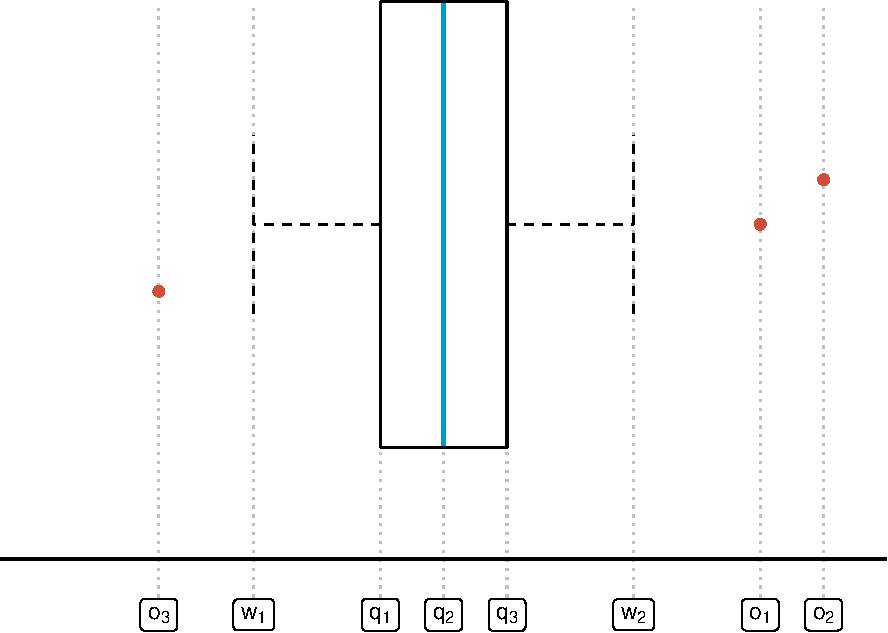
\includegraphics{Introduccion_a_Muestreo_files/figure-latex/unnamed-chunk-56-1.pdf}

La imagen anota la mediana, los cuartiles así como el rango de valores donde se sabe que no hay outliers. Finalmente la gráfica identifica los \emph{outliers} si es que hay. Para armar una gráfica de boxplot usamos la librería de \emph{ggplot2} especificando dentro de la función \texttt{ggplot} la base de datos de donde sale nuestra información:

\begin{Shaded}
\begin{Highlighting}[]
\FunctionTok{ggplot}\NormalTok{(conteo\_delitos) }\SpecialCharTok{+}
  \FunctionTok{geom\_boxplot}\NormalTok{(}\FunctionTok{aes}\NormalTok{(}\AttributeTok{x =}\NormalTok{ n))}
\end{Highlighting}
\end{Shaded}

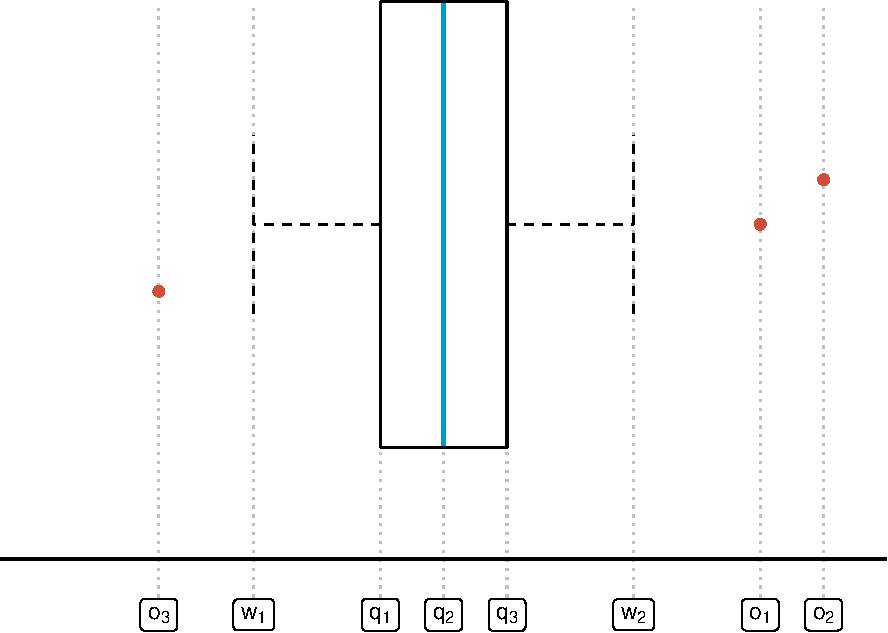
\includegraphics{Introduccion_a_Muestreo_files/figure-latex/unnamed-chunk-57-1.pdf}

la cual pone la mediana en 646 como habíamos calculado, los cuartiles en 568 y 721 respectivamente. Finalmente no presenta \emph{outliers} pues nuestro análisis previo nos mostraba que no había \emph{outliers}.

Podemos personalizar nuestra gráfica agregando títulos con la función lab:

\begin{Shaded}
\begin{Highlighting}[]
\FunctionTok{ggplot}\NormalTok{(conteo\_delitos) }\SpecialCharTok{+}
  \FunctionTok{geom\_boxplot}\NormalTok{(}\FunctionTok{aes}\NormalTok{(}\AttributeTok{x =}\NormalTok{ n)) }\SpecialCharTok{+}
  \FunctionTok{labs}\NormalTok{(}
    \AttributeTok{x =} \StringTok{"Cantidad de carpetas de investigación abiertas por día"}\NormalTok{,}
    \AttributeTok{y =} \StringTok{""}\NormalTok{,}
    \AttributeTok{title =} \StringTok{"Gráfica de cajas de los delitos en CDMX"}\NormalTok{,}
    \AttributeTok{subtitle =} \StringTok{"Fuente: Carpetas de investigación FGJ de la Ciudad de México"}\NormalTok{,}
    \AttributeTok{caption =} \StringTok{"Datos de Diciembre 2018"}
\NormalTok{  )}
\end{Highlighting}
\end{Shaded}

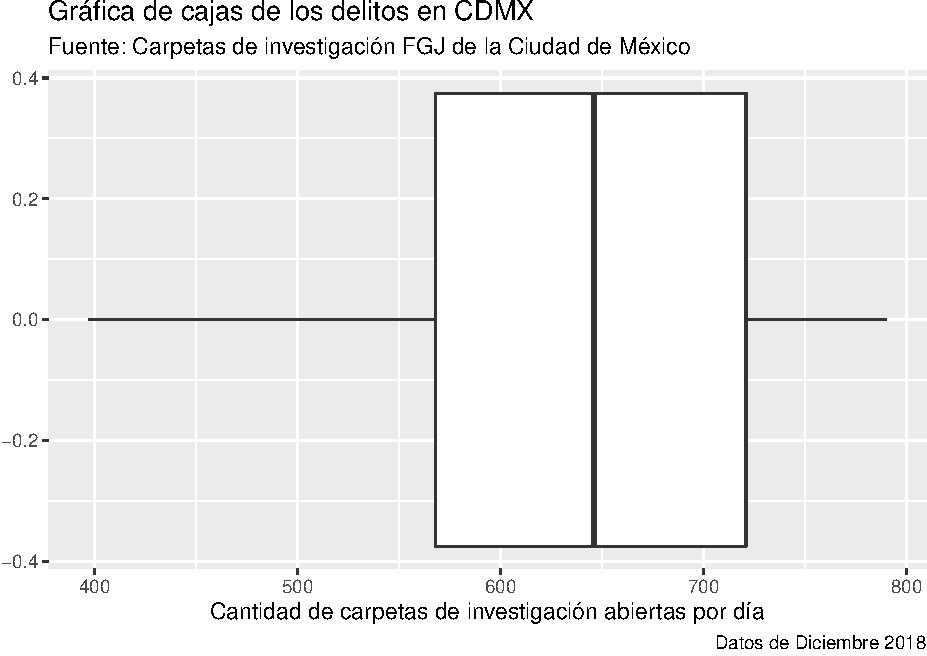
\includegraphics{Introduccion_a_Muestreo_files/figure-latex/unnamed-chunk-58-1.pdf}
Finalmente, podemos personalizar los colores de la gráfica editando directamente en el \texttt{geom\_boxplot}:

\begin{Shaded}
\begin{Highlighting}[]
\FunctionTok{ggplot}\NormalTok{(conteo\_delitos) }\SpecialCharTok{+}
  \FunctionTok{geom\_boxplot}\NormalTok{(}\FunctionTok{aes}\NormalTok{(}\AttributeTok{x =}\NormalTok{ n), }\AttributeTok{color =} \StringTok{"red"}\NormalTok{, }\AttributeTok{fill =} \StringTok{"deepskyblue4"}\NormalTok{) }\SpecialCharTok{+}
  \FunctionTok{labs}\NormalTok{(}
    \AttributeTok{x =} \StringTok{"Cantidad de carpetas de investigación abiertas por día"}\NormalTok{,}
    \AttributeTok{y =} \StringTok{""}\NormalTok{,}
    \AttributeTok{title =} \StringTok{"Gráfica de cajas de los delitos en CDMX"}\NormalTok{,}
    \AttributeTok{subtitle =} \StringTok{"Fuente: Carpetas de investigación FGJ de la Ciudad de México"}\NormalTok{,}
    \AttributeTok{caption =} \StringTok{"Datos de Diciembre 2018"}
\NormalTok{  )}
\end{Highlighting}
\end{Shaded}

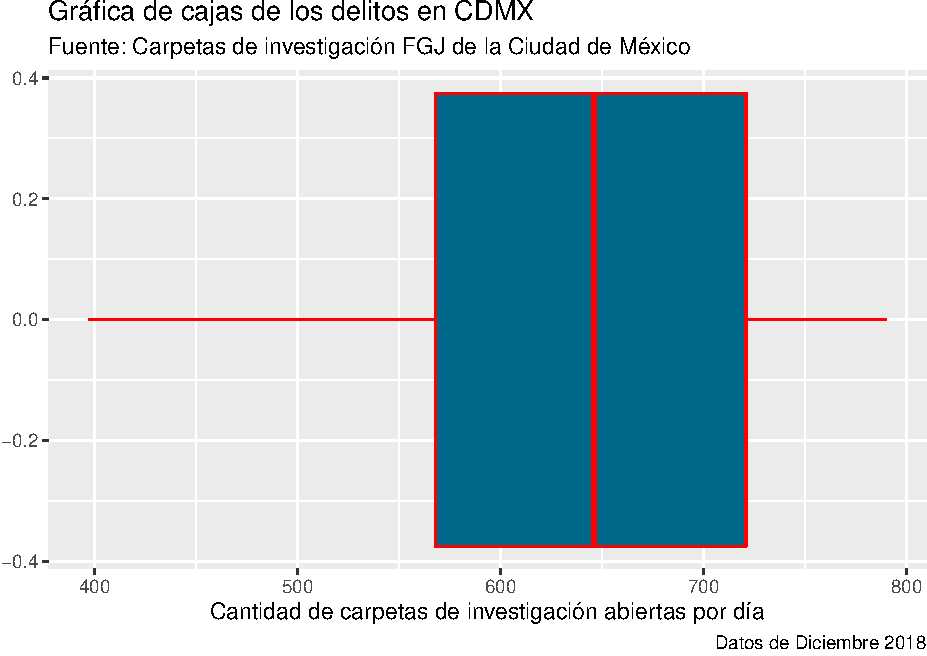
\includegraphics{Introduccion_a_Muestreo_files/figure-latex/unnamed-chunk-59-1.pdf}

\textbf{2. Gráfica de barras} Sea \(\vec{c} = (c_1, c_2, \dots, c_n)^T\) un vector de datos categóricos. Sea \(C = \{ a_i | a_i \in \vec{c} \}\) el conjunto de \(\ell\) valores únicos que se tienen registrados en el vector \(\vec{c}\). Denotamos la cantidad de veces que aparece \(a_i\) en \(\vec{c}\) como \(n_i\); es decir:

\[
n_i = \sum\limits_{k = 1}^n \mathbb{I}_{\{a_i\}}(c_k)
\]

Una gráfica de barras consiste en una representación gráfica del conjunto:
\[
\text{Barras} = \{ (a_i, n_i) | a_i \in C  \}
\]
Gráficamente:

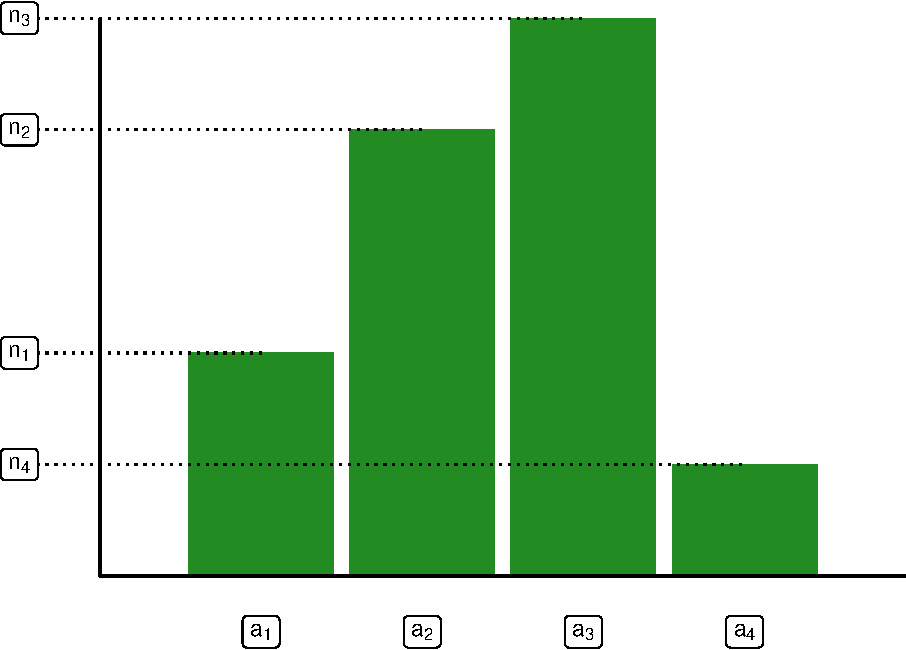
\includegraphics{Introduccion_a_Muestreo_files/figure-latex/unnamed-chunk-60-1.pdf}

Podemos crear una gráfica de barras con el comando \texttt{geom\_col} para ello creemos unas barras correspondientes al tipo de delito (sólo en delitos que \texttt{categoria\_delito} dice \texttt{ROBO}) haciendo una nueva base que cuente por delito:

\begin{Shaded}
\begin{Highlighting}[]
\NormalTok{conteo\_tipo }\OtherTok{\textless{}{-}}\NormalTok{ datos }\SpecialCharTok{\%\textgreater{}\%} \FunctionTok{filter}\NormalTok{(}\FunctionTok{str\_detect}\NormalTok{(categoria\_delito,}\StringTok{"ROBO"}\NormalTok{)) }\SpecialCharTok{\%\textgreater{}\%} 
  \FunctionTok{group\_by}\NormalTok{(delito) }\SpecialCharTok{\%\textgreater{}\%} \FunctionTok{tally}\NormalTok{()}
\end{Highlighting}
\end{Shaded}

Y hagamos la gráfica:

\begin{Shaded}
\begin{Highlighting}[]
\FunctionTok{ggplot}\NormalTok{(conteo\_tipo) }\SpecialCharTok{+}
  \FunctionTok{geom\_col}\NormalTok{(}\FunctionTok{aes}\NormalTok{(}\AttributeTok{x =}\NormalTok{ delito, }\AttributeTok{y =}\NormalTok{ n), }\AttributeTok{color =} \StringTok{"white"}\NormalTok{) }\SpecialCharTok{+}
  \FunctionTok{theme\_bw}\NormalTok{()}
\end{Highlighting}
\end{Shaded}

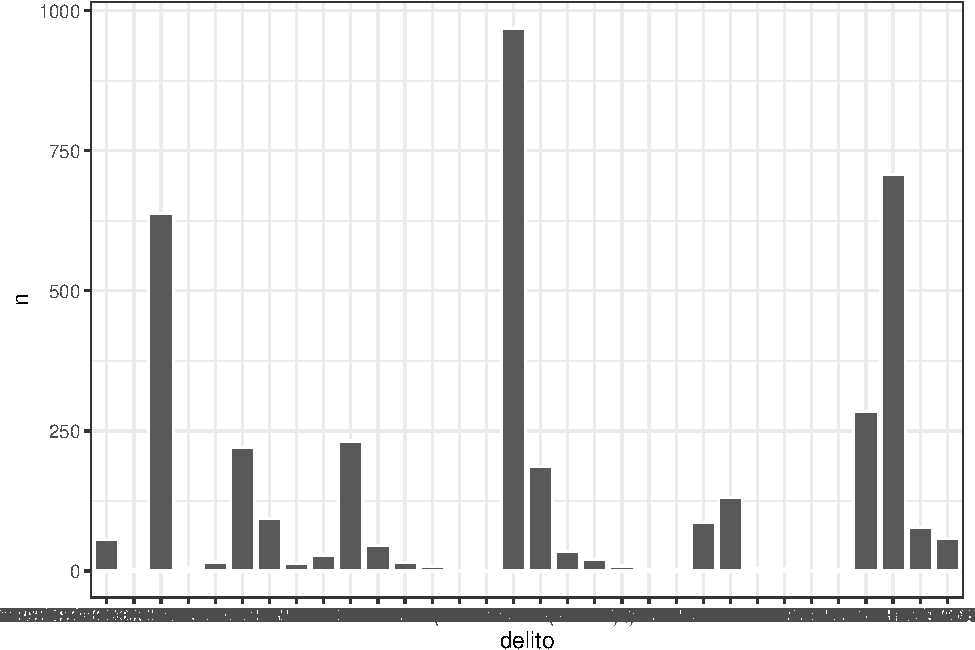
\includegraphics{Introduccion_a_Muestreo_files/figure-latex/unnamed-chunk-62-1.pdf}
Para evitar que se encime todo el texto podemos establecer un ángulo del mismo al usar \texttt{theme}:

\begin{Shaded}
\begin{Highlighting}[]
\FunctionTok{ggplot}\NormalTok{(conteo\_tipo) }\SpecialCharTok{+}
  \FunctionTok{geom\_col}\NormalTok{(}\FunctionTok{aes}\NormalTok{(}\AttributeTok{x =}\NormalTok{ delito, }\AttributeTok{y =}\NormalTok{ n), }\AttributeTok{color =} \StringTok{"white"}\NormalTok{) }\SpecialCharTok{+}
  \FunctionTok{theme\_bw}\NormalTok{() }\SpecialCharTok{+}
  \FunctionTok{theme}\NormalTok{(}\AttributeTok{axis.text.x =} \FunctionTok{element\_text}\NormalTok{(}\AttributeTok{angle =} \DecValTok{90}\NormalTok{, }\AttributeTok{size =} \DecValTok{3}\NormalTok{))}
\end{Highlighting}
\end{Shaded}

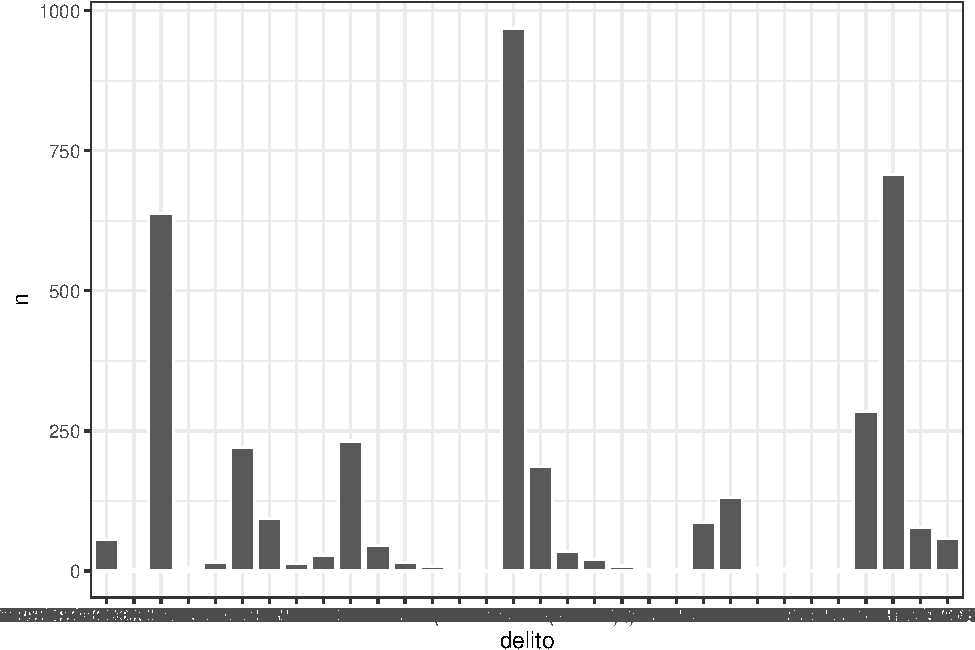
\includegraphics{Introduccion_a_Muestreo_files/figure-latex/unnamed-chunk-63-1.pdf}

\begin{quote}
\textbf{NOTA} Una mala praxis \href{https://www.data-to-viz.com/caveat/pie.html}{es usar gráficas de pay} pues es muy complicado contar una historia a partir de ellas. ¡No lo hagas!
\end{quote}

\hypertarget{gruxe1ficas-bivariadas}{%
\section{Gráficas bivariadas}\label{gruxe1ficas-bivariadas}}

\textbf{1. Gráfica de puntos (scatterplot)} Dada una matriz de datos \(Z\) consideramos dos columnas numéricas \(z_i\) y \(z_j\) (\(i \neq j\)) de dicha matriz. Sea \(\mathbb{X} = \{ (z_{i,1}, z_{j,1}), (z_{i,2}, z_{j,2}), \dots, (z_{i,n}, z_{j,n}) \}\) el conjunto de parejas ordenadas correspondientes a dichas columnas. Una gráfica de puntos consiste en la proyección de dichos puntos sobre \(\mathbb{R}^2\). Para generarla en \texttt{R} podemos usar \texttt{ggplot}:

\begin{Shaded}
\begin{Highlighting}[]
\FunctionTok{ggplot}\NormalTok{(datos) }\SpecialCharTok{+}
  \FunctionTok{geom\_point}\NormalTok{(}\FunctionTok{aes}\NormalTok{(}\AttributeTok{x =}\NormalTok{ longitud, }\AttributeTok{y =}\NormalTok{ latitud), }\AttributeTok{size =} \DecValTok{1}\NormalTok{, }\AttributeTok{color =} \StringTok{"purple"}\NormalTok{,}
             \AttributeTok{alpha =} \FloatTok{0.2}\NormalTok{)}
\end{Highlighting}
\end{Shaded}

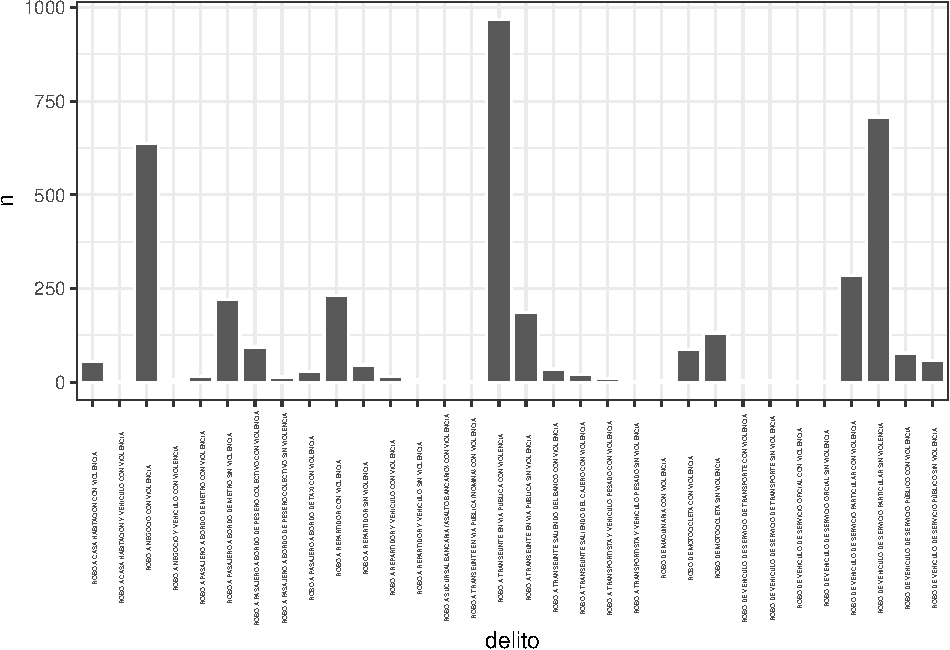
\includegraphics{Introduccion_a_Muestreo_files/figure-latex/unnamed-chunk-64-1.pdf}
donde los parámetros \texttt{size} establecen el tamaño del punto, \texttt{color} su color y \texttt{alpha} su nivel de transparencia (\(0 \leq \alpha \leq 1\)).

\textbf{2. Gráfica de líneas (lineplot)} Dada una matriz de datos \(Z\) consideramos dos columnas numéricas \(z_i\) y \(z_j\) (\(i \neq j\)) de dicha matriz. Sea \(\mathbb{X} = \{ (z_{i,1}, z_{j,1}), (z_{i,2}, z_{j,2}), \dots, (z_{i,n}, z_{j,n}) \}\) el conjunto de parejas ordenadas correspondientes a dichas columnas. Para evitar confusión de subíndices escribiré a las \(z_i\) como \(x\) y a las \(z_j\) como \(y\) de tal forma que \(\mathbb{X} = \{ (x_1, y_1), (x_2, y_2), \dots, (x_n, y_n) \}\)
Supongamos, sin pérdida de generalidad que los datos están ordenados según las \(x\): \(x_1 \leq x_2 \leq \dots \leq x_n\). Sea \(f\) la función de interpolación lineal dada por:
\[
f(x) = \begin{cases}
y_1 + \frac{y_2 - y_1}{x_2 - x_1} (x -x_1) & \text{ si } x_1 \leq x \leq x_2 \\
\vdots \\
y_{k-1} + \frac{y_k - y_{k-1}}{x_k - x_{k-1}} (x -x_{k-1}) & \text{ si } x_{k-1} \leq x \leq x_k \\
\vdots \\
y_{n-1} + \frac{y_{n} - y_{n-1}}{x_n - x_{n-1}} (x -x_{n-1}) & \text{ si } x_{n-1} \leq x \leq x_n \\
\end{cases}
\]
Una gráfica de líneas corresponde a la representación gráfica del conjunto
\[
\textrm{Gr}_f = \Big\{ \big(x, f(x)\big) |  x_1 \leq x \leq x_n \Big\}
\]
De manera un poco más intuitiva notamos que si tenemos, por ejemplo, \(\mathbb{X} = \{(x_1, y_1),(x_2, y_2), (x_3, y_3), (x_4, y_4)\}\) una gráfica de líneas se construye interpolando una línea entre \((x_1, y_1)\) y \((x_2, y_2)\), otra línea entre \((x_2, y_2)\) y \((x_3, y_3)\) y, finalmente, otra recta entre \((x_3, y_3)\) y \((x_4, y_4)\). Usando la ecuación de la línea
\[
y = \frac{y_2 - y_1}{x_2 - x_1} (x - x_1) + y_1
\]
interpolamos cada uno de los puntos como en la gráfica siguiente:

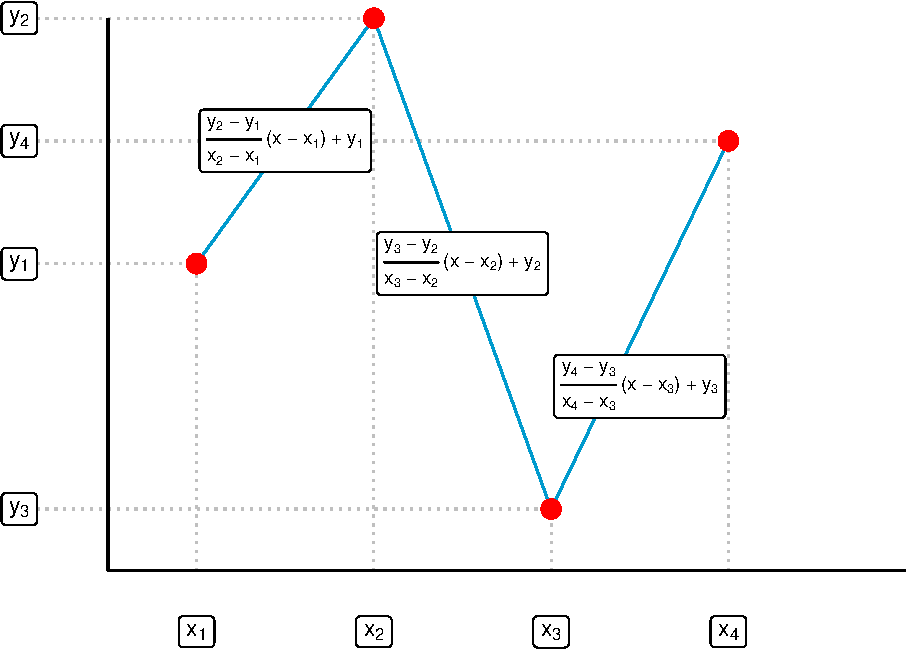
\includegraphics{Introduccion_a_Muestreo_files/figure-latex/unnamed-chunk-65-1.pdf}
Para realizar una gráfica de líneas podemos usar de nuevo ggplot2 con la opción de \texttt{geom\_line}:

\begin{Shaded}
\begin{Highlighting}[]
\FunctionTok{ggplot}\NormalTok{(conteo\_delitos) }\SpecialCharTok{+} 
  \FunctionTok{geom\_line}\NormalTok{(}\FunctionTok{aes}\NormalTok{(}\AttributeTok{x =}\NormalTok{ fecha, }\AttributeTok{y =}\NormalTok{ n))}
\end{Highlighting}
\end{Shaded}

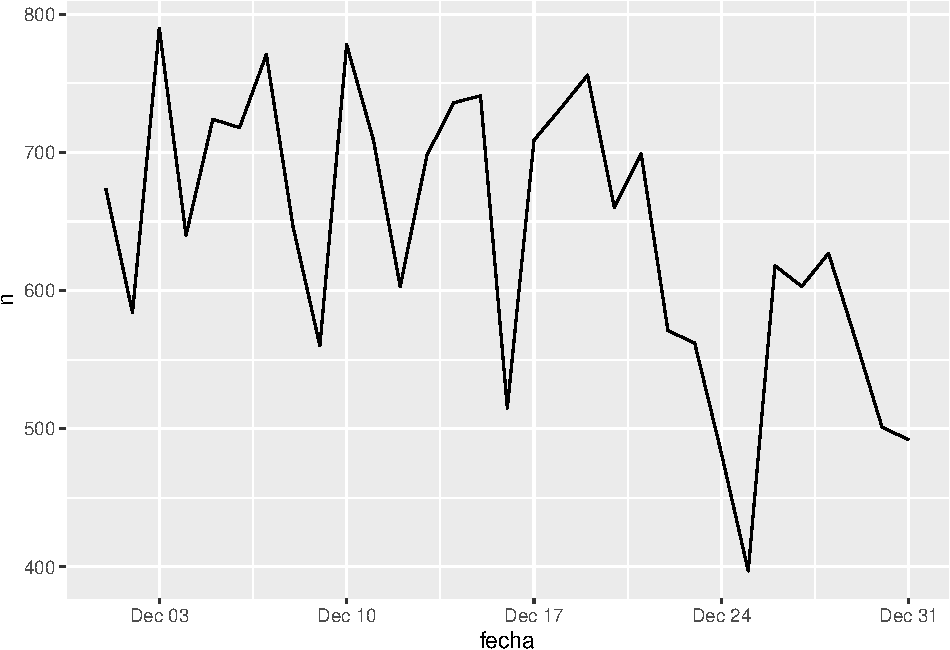
\includegraphics{Introduccion_a_Muestreo_files/figure-latex/unnamed-chunk-66-1.pdf}

Podemos cambiar el tema y agregar puntos de otro color para que nuestra gráfica se vea más bonita:

\begin{Shaded}
\begin{Highlighting}[]
\FunctionTok{ggplot}\NormalTok{(conteo\_delitos) }\SpecialCharTok{+} 
  \FunctionTok{geom\_line}\NormalTok{(}\FunctionTok{aes}\NormalTok{(}\AttributeTok{x =}\NormalTok{ fecha, }\AttributeTok{y =}\NormalTok{ n)) }\SpecialCharTok{+}
  \FunctionTok{geom\_point}\NormalTok{(}\FunctionTok{aes}\NormalTok{(}\AttributeTok{x =}\NormalTok{ fecha, }\AttributeTok{y =}\NormalTok{ n), }\AttributeTok{color =} \StringTok{"red"}\NormalTok{, }\AttributeTok{size =} \DecValTok{3}\NormalTok{) }\SpecialCharTok{+}
  \FunctionTok{theme\_classic}\NormalTok{() }\SpecialCharTok{+}
  \FunctionTok{labs}\NormalTok{(}
    \AttributeTok{x =} \StringTok{"Fecha de apertura de la carpeta de investigación"}\NormalTok{,}
    \AttributeTok{y =} \StringTok{"Cantidad de carpetas de investigación en FGJ"}
\NormalTok{  )}
\end{Highlighting}
\end{Shaded}

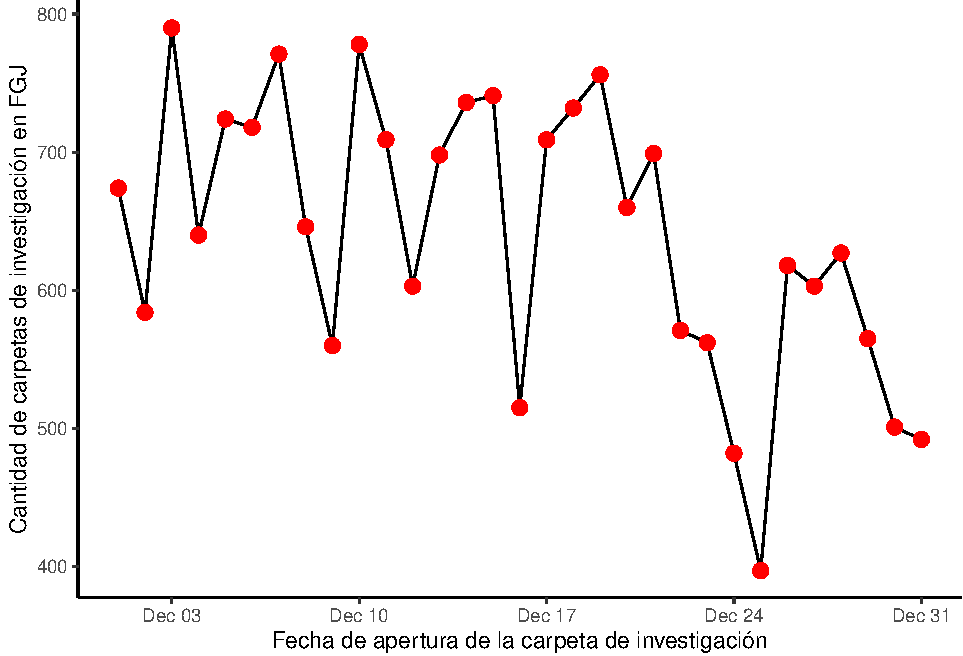
\includegraphics{Introduccion_a_Muestreo_files/figure-latex/unnamed-chunk-67-1.pdf}
Finalmente con \texttt{geom\_label} podemos agregar anotaciones a nuestra gráfica:

\begin{Shaded}
\begin{Highlighting}[]
\FunctionTok{ggplot}\NormalTok{(conteo\_delitos) }\SpecialCharTok{+} 
  \FunctionTok{geom\_line}\NormalTok{(}\FunctionTok{aes}\NormalTok{(}\AttributeTok{x =}\NormalTok{ fecha, }\AttributeTok{y =}\NormalTok{ n)) }\SpecialCharTok{+}
  \FunctionTok{geom\_point}\NormalTok{(}\FunctionTok{aes}\NormalTok{(}\AttributeTok{x =}\NormalTok{ fecha, }\AttributeTok{y =}\NormalTok{ n), }\AttributeTok{color =} \StringTok{"red"}\NormalTok{, }\AttributeTok{size =} \DecValTok{3}\NormalTok{) }\SpecialCharTok{+}
  \FunctionTok{theme\_classic}\NormalTok{() }\SpecialCharTok{+}
  \FunctionTok{labs}\NormalTok{(}
    \AttributeTok{x =} \StringTok{"Fecha de apertura de la carpeta de investigación"}\NormalTok{,}
    \AttributeTok{y =} \StringTok{"Cantidad de carpetas de investigación en FGJ"}
\NormalTok{  ) }\SpecialCharTok{+}
  \FunctionTok{geom\_label}\NormalTok{(}\FunctionTok{aes}\NormalTok{(}\AttributeTok{x =} \FunctionTok{dmy}\NormalTok{(}\StringTok{"25/12/2018"}\NormalTok{), }\AttributeTok{y =} \DecValTok{425}\NormalTok{), }\AttributeTok{label =} \StringTok{"Efecto de Navidad"}\NormalTok{)}
\end{Highlighting}
\end{Shaded}

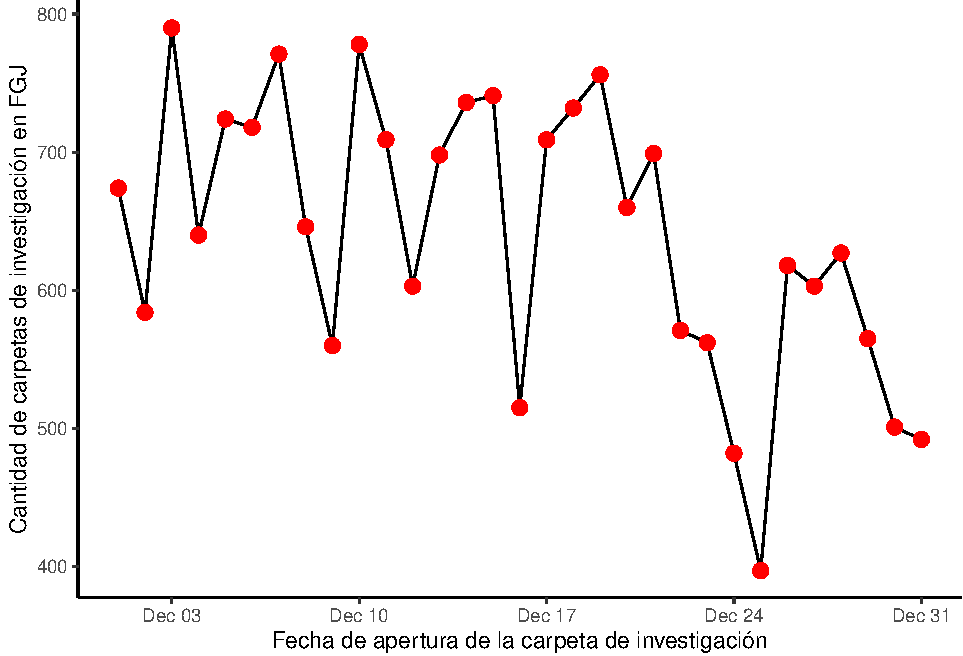
\includegraphics{Introduccion_a_Muestreo_files/figure-latex/unnamed-chunk-68-1.pdf}

\hypertarget{ejercicio-1}{%
\subsection{Ejercicio}\label{ejercicio-1}}

Utiliza las siguiente bases de datos para replicar exactamente el formato de las gráficas que se muestran abajo de las bases. No todo viene en estas notas, la idea es que investigues y para ello te sugiero \href{https://ggplot2-book.org}{consultar este libro}

\emph{Gráfica de barras}

\begin{Shaded}
\begin{Highlighting}[]
\NormalTok{datos.barras }\OtherTok{\textless{}{-}} \FunctionTok{data.frame}\NormalTok{(}\AttributeTok{Pais =} \FunctionTok{c}\NormalTok{(}\StringTok{"EEUU"}\NormalTok{,}\StringTok{"Canadá"}\NormalTok{,}\StringTok{"México"}\NormalTok{), }
                           \AttributeTok{PIB =} \FunctionTok{c}\NormalTok{(}\FloatTok{20.54}\NormalTok{, }\FloatTok{17.13}\NormalTok{, }\FloatTok{1.21}\NormalTok{))}
\end{Highlighting}
\end{Shaded}

Los colores usados son \texttt{firebrick}, \texttt{deepskyblue3} y \texttt{forestgreen}:

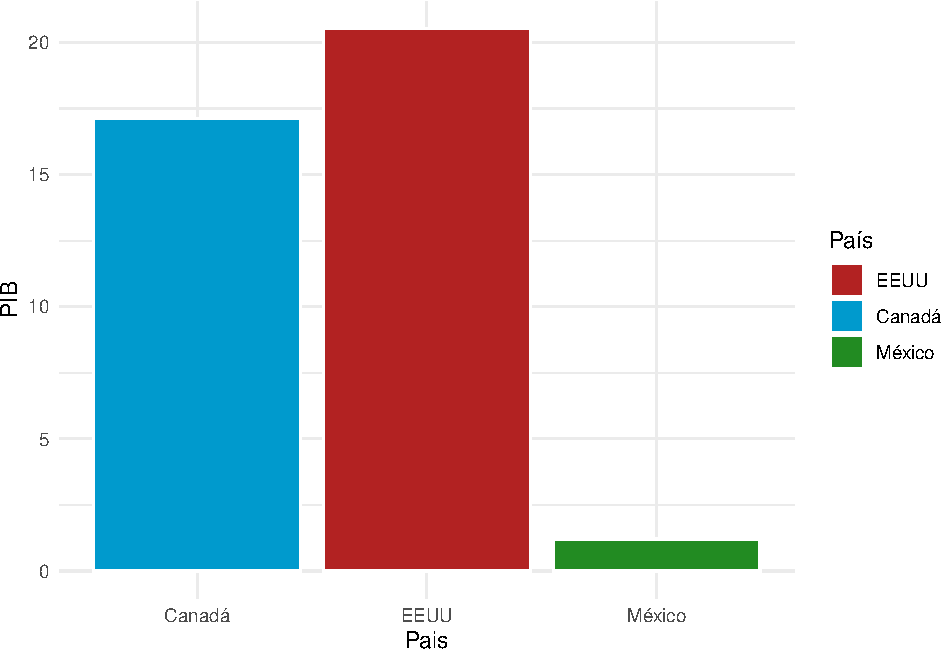
\includegraphics{Introduccion_a_Muestreo_files/figure-latex/unnamed-chunk-70-1.pdf}
\emph{Línea}

\begin{Shaded}
\begin{Highlighting}[]
\NormalTok{x }\OtherTok{\textless{}{-}} \FunctionTok{seq}\NormalTok{(}\SpecialCharTok{{-}}\DecValTok{2}\SpecialCharTok{*}\NormalTok{pi, }\DecValTok{2}\SpecialCharTok{*}\NormalTok{pi, }\AttributeTok{length.out =} \DecValTok{100}\NormalTok{)}
\NormalTok{datos.linea }\OtherTok{\textless{}{-}} \FunctionTok{data.frame}\NormalTok{(}\AttributeTok{x =}\NormalTok{ x, }\AttributeTok{y =} \FunctionTok{sin}\NormalTok{(x))}
\end{Highlighting}
\end{Shaded}

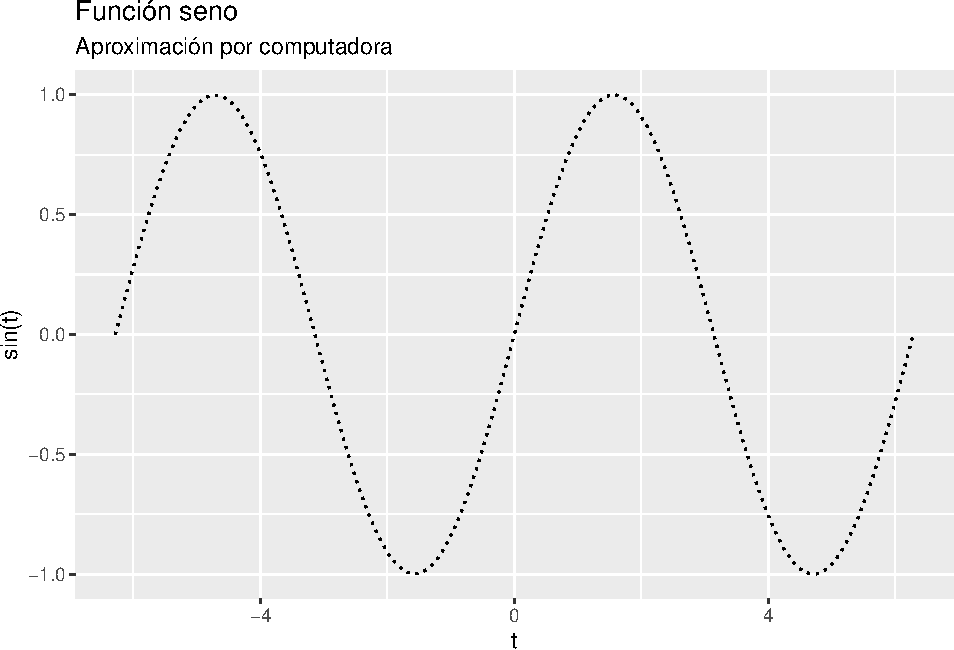
\includegraphics{Introduccion_a_Muestreo_files/figure-latex/unnamed-chunk-72-1.pdf}

\emph{Boxplot}

\begin{Shaded}
\begin{Highlighting}[]
\NormalTok{x }\OtherTok{\textless{}{-}} \FunctionTok{c}\NormalTok{(}\DecValTok{1}\NormalTok{,}\DecValTok{10}\NormalTok{, }\DecValTok{100}\NormalTok{, }\SpecialCharTok{{-}}\DecValTok{2}\NormalTok{, }\DecValTok{3}\NormalTok{, }\DecValTok{5}\NormalTok{, }\DecValTok{6}\NormalTok{, }\DecValTok{12}\NormalTok{, }\SpecialCharTok{{-}}\DecValTok{8}\NormalTok{, }\DecValTok{31}\NormalTok{, }\DecValTok{2}\NormalTok{, pi, }\DecValTok{3}\NormalTok{)}
\NormalTok{datos.linea }\OtherTok{\textless{}{-}} \FunctionTok{data.frame}\NormalTok{(}\AttributeTok{Dientes =}\NormalTok{ x)}
\end{Highlighting}
\end{Shaded}

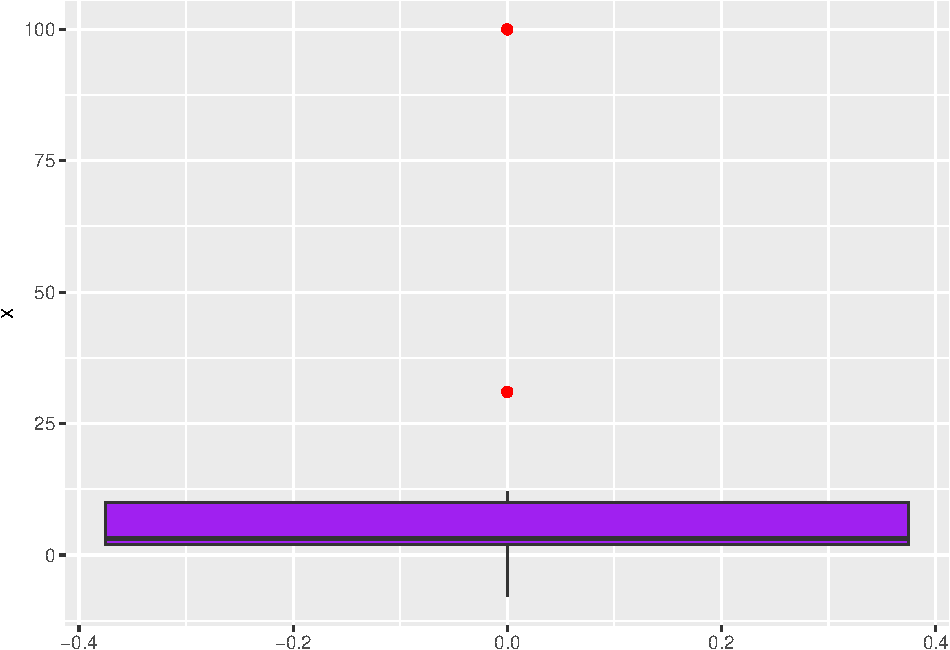
\includegraphics{Introduccion_a_Muestreo_files/figure-latex/unnamed-chunk-74-1.pdf}

\emph{Puntos}

\begin{Shaded}
\begin{Highlighting}[]
\NormalTok{datos.arbol }\OtherTok{\textless{}{-}} \FunctionTok{data.frame}\NormalTok{(}\AttributeTok{altura =} \FunctionTok{c}\NormalTok{(}\FloatTok{1.7}\NormalTok{, }\FloatTok{1.4}\NormalTok{, }\FloatTok{1.8}\NormalTok{, }\FloatTok{1.9}\NormalTok{, }\FloatTok{1.5}\NormalTok{, }\FloatTok{1.7}\NormalTok{,}
                                     \FloatTok{1.6}\NormalTok{, }\FloatTok{1.8}\NormalTok{, }\FloatTok{1.7}\NormalTok{, }\FloatTok{1.8}\NormalTok{),}
                          \AttributeTok{ancho =} \FunctionTok{c}\NormalTok{(}\FloatTok{1.2}\NormalTok{, }\FloatTok{1.4}\NormalTok{, }\FloatTok{1.2}\NormalTok{, }\DecValTok{1}\NormalTok{, }\FloatTok{1.5}\NormalTok{, }\FloatTok{1.7}\NormalTok{, }\FloatTok{1.6}\NormalTok{,}
                                    \FloatTok{1.2}\NormalTok{, }\FloatTok{1.2}\NormalTok{, }\DecValTok{1}\NormalTok{),}
                          \AttributeTok{tipo =} \FunctionTok{c}\NormalTok{(}\StringTok{"Pino"}\NormalTok{,}\StringTok{"Sauce"}\NormalTok{,}\StringTok{"Sauce"}\NormalTok{,}\StringTok{"Sauce"}\NormalTok{,}\StringTok{"Pino"}\NormalTok{,}
                                   \StringTok{"Pino"}\NormalTok{,}\StringTok{"Pino"}\NormalTok{,}\StringTok{"Sauce"}\NormalTok{,}\StringTok{"Sauce"}\NormalTok{,}\StringTok{"Sauce"}\NormalTok{))}
\end{Highlighting}
\end{Shaded}

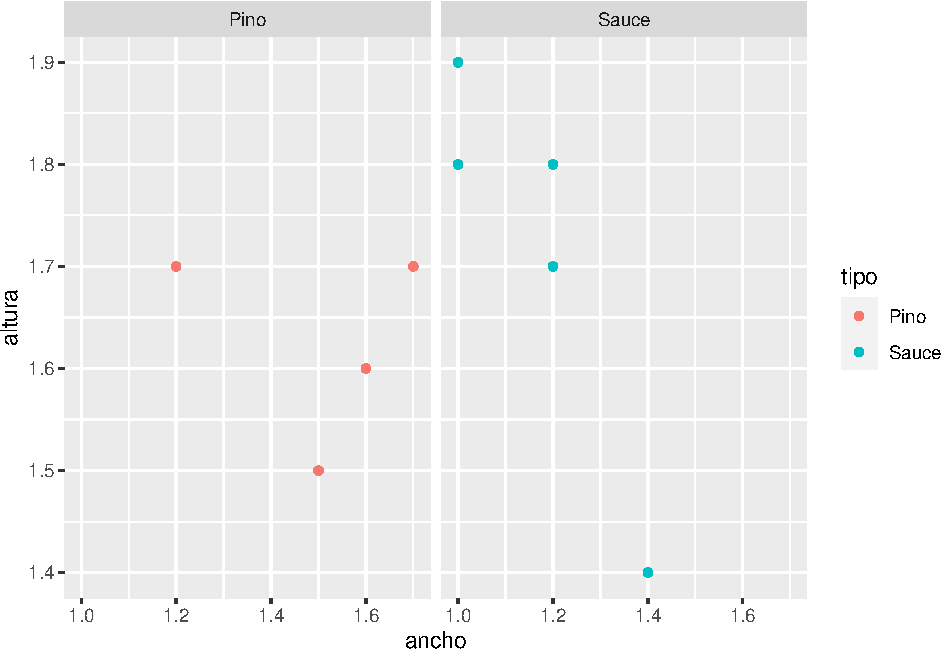
\includegraphics{Introduccion_a_Muestreo_files/figure-latex/unnamed-chunk-76-1.pdf}

\hypertarget{estaduxedsticos-bivariados}{%
\section{Estadísticos bivariados}\label{estaduxedsticos-bivariados}}

\textbf{NOTACIÓN} Para esta sección vamos a considerar dos (vectores) columnas de la matriz de datos \(Z\) y los denominaremos \(\vec{x}\) y \(\vec{y}\) (en lugar de \(z_i\) y \(z_j\)). En particular, denotaremos \(\mathcal{X} = \{ a_{i, x } | a_{i,x} \in \vec{x} \}\) el conjunto de valores únicos del vector \(\vec{x}\) y \(\mathcal{Y} = \{ a_{y ,j} | a_{y ,j} \in \vec{y} \}\) el conjunto de valores únicos de \(\vec{y}\). La cardinalidad de dichos conjuntos es \(\ell_{x}\) y \(\ell_{y}\) respectivamente. Finalmente, definimos el conteo de cuántas veces aparece el valor \(a_{i,x }\) (respectivamente el \(a_{y ,j}\)) en los vectores \(\vec{x}\) (respectivamente \(\vec{y}\)) como:
\begin{equation}
\begin{aligned}
n_{i,x } & = \sum\limits_{k=1}^{n} \mathbb{I}_{\{ a_{i,x } \}}(x_k) \\
n_{y ,j} & = \sum\limits_{k=1}^{n} \mathbb{I}_{\{ a_{y ,j} \}}(y_k)
\end{aligned}
\end{equation}
para \(1 \leq i \leq \ell_{x}\) y \(1 \leq j \leq \ell_{y}\).

\begin{quote}
Por poner un ejemplo, considera el siguiente conjunto de datos:

\begin{table}
\centering
\begin{tabular}{l|l}
\hline
x & y\\
\hline
\cellcolor{gray!6}{Rojo} & \cellcolor{gray!6}{Coche}\\
\hline
Azul & Taza\\
\hline
\cellcolor{gray!6}{Verde} & \cellcolor{gray!6}{Árbol}\\
\hline
Rojo & Taza\\
\hline
\cellcolor{gray!6}{Verde} & \cellcolor{gray!6}{Libro}\\
\hline
\end{tabular}
\end{table}

En este sentido el vector es \(\vec{x} = (\text{Rojo},\text{Azul},\text{Verde},\text{Rojo},\text{Verde})^T\) mientras que el conjunto de valores únicos asociados está dado por \(\mathcal{X} = \{ \text{Rojo},\text{Azul},\text{Verde} \}\). En este sentido (siguiendo el conjunto) se tiene que \(a_{1,x} = \text{Rojo}\), \(a_{2,x} = \text{Azul}\) y \(a_{3,x } = \text{Verde}\) mientras que (siguiendo el vector) se observa \(x_1 = \text{Rojo}\), \(x_2 = \text{Azul}\), \(x_3 = \text{Verde}\), \(x_4 = \text{Rojo}\), \(x_5 = \text{Verde}\). Finalmente notamos que el conteo de veces que aparece cada cosa es: \(n_{1,x} = 2\) (aparece el \(a_{1, x}\) que es rojo dos veces), \(n_{2,x} = 1\) y \(n_{3,x } = 2\) (el azul y verde dados por \(a_{2,x}\) y \(a_{3,x}\) respectivamente aparecen una vez para azul y dos veces para verde). Por otro lado, \(\vec{y} = (\text{Coche},\text{Taza},\text{Árbol},\text{Taza},\text{Libro})^T\) con su conjunto de valores únicos \(\mathcal{Y} = \{ \text{Coche},\text{Taza},\text{Árbol}, \text{Libro} \}\). Para el caso de \(\vec{y}\) se tiene que \(y_1 = \text{Coche}\), \(y_2 = \text{Taza}\), \(y_3 = \text{Árbol}\), \(y_4 = \text{Taza}\), \(y_5 = \text{Libro}\) mientras que en el caso de valores únicos \(a_{y, 1} = \text{Coche}\), \(a_{y, 2} = \text{Taza}\), \(a_{y, 3} = \text{Árbol}\), \(a_{\cdot, 4} = \text{Libro}\). Los conteos asociados son: \(n_{y,1} = n_{y,3} = n_{y,4} = 1\) (aparecen el coche, el árbol y el libro una vez) mientras que \(n_{y,2} = 2\) representa que la taza está dos veces.
\end{quote}

Por otro lado denotamos a la submatriz de \(Z\) compuesta solamente por las columnas \(\vec{x}\) y \(\vec{y}\) como:

\[
Z_{(x,y)} = 
\begin{pmatrix}
x_1 & y_1 \\
x_2 & y_2 \\
\vdots & \vdots \\
x_n & y_n \\
\end{pmatrix}
\]
Sea \(\mathcal{X}\times\mathcal{Y} = \{ a_{i,j} = (x_i,y_j) | x_i \in \mathcal{X} \quad \& \quad y_j \in \mathcal{Y}\}\) el conjunto de observaciones únicas \emph{posibles} de las parejas \((x,y)\) (todas las permutaciones). Finalmente, el conteo de cuántas veces aparece el vector bivariado \(a_{i,j}\) en los datos está dado por:
\[
n_{i,j} = \sum\limits_{k = 1}^{n}  \mathbb{I}_{\{ a_{i,j} \}}\big( (x_k, y_k) \big)
\]
En el ejemplo anterior, la tabla se vería:

\begin{verbatim}
## Warning: Setting row names on a tibble is deprecated.
\end{verbatim}

\begin{table}
\centering
\begin{tabular}{l|r|r|r|r|r}
\hline
  & Coche & Taza & Árbol & Libro & Total (fila)\\
\hline
\cellcolor{gray!6}{Rojo} & \cellcolor{gray!6}{1} & \cellcolor{gray!6}{1} & \cellcolor{gray!6}{0} & \cellcolor{gray!6}{0} & \cellcolor{gray!6}{2}\\
\hline
Azul & 0 & 1 & 0 & 0 & 1\\
\hline
\cellcolor{gray!6}{Verde} & \cellcolor{gray!6}{0} & \cellcolor{gray!6}{0} & \cellcolor{gray!6}{1} & \cellcolor{gray!6}{1} & \cellcolor{gray!6}{2}\\
\hline
Total (columna) & 1 & 2 & 1 & 1 & 5\\
\hline
\end{tabular}
\end{table}

Una excelente referencia para esta sección es el capítulo 4 de \protect\hyperlink{ref-peck2015introduction}{Peck, Olsen, and Devore} (\protect\hyperlink{ref-peck2015introduction}{2015}).

\textbf{1. Tabla de contingencia }
Para \(\vec{x}\), \(\vec{y}\) definidas como al inicio de la sección (y siguiendo la notación anterior), definimos una tabla de contingencia como la matriz \(N_{x,y}\) dada por:
\[
N_{x,y} = \begin{pmatrix}
n_{1,1} & n_{1,2} & \dots & n_{1, \ell_y} \\
n_{2,1} & n_{2,2} & \dots & n_{2, \ell_y} \\
\vdots  & \vdots  & \ddots & \vdots \\
n_{\ell_x,1} & n_{\ell_x,2} & \dots & n_{\ell_x, \ell_y} \\
\end{pmatrix}
\]
Al vector \(n_x = (n_{1,x}, n_{2,x}, \dots, n_{\ell_x,x})^T\) se le conoce como \textbf{distribución frecuencial (observada) marginal} de \(\vec{x}\) mientras que \(n_y = (n_{y,1}, n_{y,2}, \dots, n_{y,\ell_y})^T\) es la \textbf{distribución frecuencial (observada) marginal} de \(\vec{y}\).

Una tabla de contingencia representa el conteo de observaciones de una variable ajustado por la otra. Para crear una tabla de contingencia en \texttt{R} podemos usar el mismo comando \texttt{table} que ya usamos antes pero esta vez introduciendo dos vectores como en el siguiente ejemplo donde notamos alcaldía contra año del registo:

\begin{Shaded}
\begin{Highlighting}[]
\FunctionTok{table}\NormalTok{(datos}\SpecialCharTok{$}\NormalTok{alcaldia\_hechos, datos}\SpecialCharTok{$}\NormalTok{ao\_inicio)}
\end{Highlighting}
\end{Shaded}

\begin{verbatim}
##             
##              2018 2019
##   VERACRUZ      0    1
##   VILLAGRAN     1    0
##   XALATLACO     2    0
##   XOCHIMILCO  465  115
##   XOCHITEPEC    1    0
##   ZACATECAS     0    2
\end{verbatim}

Para agregar las distribuciones frecuenciales marginales a la tabla podemos usar el comando \texttt{addmargins}:

\begin{Shaded}
\begin{Highlighting}[]
\FunctionTok{addmargins}\NormalTok{(}\FunctionTok{table}\NormalTok{(datos}\SpecialCharTok{$}\NormalTok{alcaldia\_hechos, datos}\SpecialCharTok{$}\NormalTok{ao\_inicio))}
\end{Highlighting}
\end{Shaded}

\begin{verbatim}
##             
##               2018  2019   Sum
##   VILLAGRAN      1     0     1
##   XALATLACO      2     0     2
##   XOCHIMILCO   465   115   580
##   XOCHITEPEC     1     0     1
##   ZACATECAS      0     2     2
##   Sum        15952  3896 19848
\end{verbatim}

\textbf{2. Tabla de frecuencias}

Una tabla de frecuencia es la matriz \(\text{Freq}_{x,y}\) dada por:
\[
\text{Freq}_{x,y} = \begin{pmatrix}
f_{1,1} & f_{1,2} & \dots & f_{1, \ell_y} \\
f_{2,1} & f_{2,2} & \dots & f_{2, \ell_y} \\
\vdots  & \vdots  & \ddots & \vdots \\
f_{\ell_x,1} & f_{\ell_x,2} & \dots & f_{\ell_x, \ell_y} \\
\end{pmatrix}
\]

donde \(f_{i,j} = \frac{n_{i,j}}{n}\) representa la frecuencia relativa de la observación de \((a_{i,x}, a_{y,j})\) \emph{i.e.} cuánto representa del total. Al vector \(f_{x} = (f_{1,x}, f_{2,x}, \dots, f_{\ell_x,x})^T\) se le conoce como \textbf{la distribución frecuencial marginal relativa} de \(\vec{x}\). Análogamente para \(y\) se tiene \textbf{la distribución frecuencial marginal relativa} de \(\vec{y}\) dada por: \(f_{y} = (f_{y,1}, f_{y,2}, \dots, f_{y,\ell_y})^T\). Las entradas de dichos vectores son de la forma \(f_{i,x} = n_{i,x}/n\) y \(f_{y,j} = n_{y,j}/n\).

En \texttt{R} podemos obtener las frecuencias mediante \texttt{prop.table}:

\begin{Shaded}
\begin{Highlighting}[]
\FunctionTok{prop.table}\NormalTok{(}\FunctionTok{table}\NormalTok{(datos}\SpecialCharTok{$}\NormalTok{alcaldia\_hechos, datos}\SpecialCharTok{$}\NormalTok{ao\_inicio))}
\end{Highlighting}
\end{Shaded}

\begin{verbatim}
##             
##                      2018         2019
##   VERACRUZ   0.000000e+00 5.038291e-05
##   VILLAGRAN  5.038291e-05 0.000000e+00
##   XALATLACO  1.007658e-04 0.000000e+00
##   XOCHIMILCO 2.342805e-02 5.794035e-03
##   XOCHITEPEC 5.038291e-05 0.000000e+00
##   ZACATECAS  0.000000e+00 1.007658e-04
\end{verbatim}

Así mismo, podemos agregar las marginales:

\begin{Shaded}
\begin{Highlighting}[]
\FunctionTok{addmargins}\NormalTok{(}\FunctionTok{prop.table}\NormalTok{(}\FunctionTok{table}\NormalTok{(datos}\SpecialCharTok{$}\NormalTok{alcaldia\_hechos, datos}\SpecialCharTok{$}\NormalTok{ao\_inicio)))}
\end{Highlighting}
\end{Shaded}

\begin{verbatim}
##             
##                      2018         2019          Sum
##   VILLAGRAN  5.038291e-05 0.000000e+00 5.038291e-05
##   XALATLACO  1.007658e-04 0.000000e+00 1.007658e-04
##   XOCHIMILCO 2.342805e-02 5.794035e-03 2.922209e-02
##   XOCHITEPEC 5.038291e-05 0.000000e+00 5.038291e-05
##   ZACATECAS  0.000000e+00 1.007658e-04 1.007658e-04
##   Sum        8.037082e-01 1.962918e-01 1.000000e+00
\end{verbatim}

\textbf{3. Riesgo Relativo (discreto)}
Para definir Riesgo Relativo empezaremos por un ejemplo. Tomamos la tabla \eqref{fumador} donde se guardó un registro de personas según si fumaban o no así como si dichas personas desarrollaron o no enfisema pulmonar.

\begin{verbatim}
## Warning: Setting row names on a tibble is deprecated.
\end{verbatim}

\begin{table}
\centering
\begin{tabular}{l|r|r}
\hline
  & FUMA & NO FUMA\\
\hline
\cellcolor{gray!6}{Con enfisema} & \cellcolor{gray!6}{100} & \cellcolor{gray!6}{40}\\
\hline
Sin enfisema & 30 & 50\\
\hline
\end{tabular}
\end{table}

Si quisiéramos analizar la hipótesis de que FUMAR está asociado con ENFISEMA tendríamos que ver, dentro de la población de fumadores (FUMAR = SÍ) cuántos hay (proporcionalmente) con ENFISEMA. La hipótesis es que si no hubiera relación, saldría que las proporciones de fumadores con y sin enfisema serían \(50\%\) cada una. La proporción de fumadores con enfisema está dada por \(100/130\) mientras que la de no fumadores con enfisema es \(40/90\). El riesgo relativo (intuitivamente). se define como la división entre ambas proporciones:
\[
\text{Riesgo Relativo de Enfisema} = \dfrac{\frac{\text{Expuestos enfermos}}{\text{Total de expuestos}}}{\frac{\text{No Expuestos enfermos}}{\text{Total de no expuestos}}} =  \dfrac{100/130}{40/90} \approx 1.73
\]
Lo que se interpreta como que los fumadores tienen \(1.73\) veces más riesgo de desarrollar enfisema que los no fumadores ya que si despejamos de la fórmula anterior:
\[
\frac{\text{Expuestos enfermos}}{\text{Total de expuestos}}   \approx 1.73 \times \frac{\text{No Expuestos enfermos}}{\text{Total de no expuestos}}
\]
De manera general, dadas dos vectores lógicos \(\vec{x}\) (interpretada como el resultado) y \(\vec{y}\) (interpretada como la exposición) con una tabla de contingencia y frecuencias marginales dadas por la tabla:

\begin{verbatim}
## Warning: Setting row names on a tibble is deprecated.
\end{verbatim}

\begin{table}
\centering
\begin{tabular}{l|l|l}
\hline
  & Expuesto (y) & NO expuesto (y)\\
\hline
\cellcolor{gray!6}{Resultado (x)} & \cellcolor{gray!6}{a} & \cellcolor{gray!6}{b}\\
\hline
Sin resultado (x) & c & d\\
\hline
\end{tabular}
\end{table}

definimos el riesgo relativo de \(\vec{x}\) dado \(\vec{y}\) como:
\[
RR(\vec{x}|\vec{y}) = \dfrac{\frac{a}{a + c}}{\frac{b}{b + d}}
\]
Mientras que el riesgo relativo de no \(\vec{x}\) dado \(\vec{y}\) está dado por:
\[
RR(\neg \vec{x}|\vec{y}) = \dfrac{\frac{c}{a + c}}{\frac{d}{b + d}}
\]

La base de datos de los delitos no contiene información suficiente para poder calcular un riesgo relativo pero podemos crear la base de datos correspondiente a la tabla \ref{fumador} como sigue:

\begin{Shaded}
\begin{Highlighting}[]
\NormalTok{fumadores }\OtherTok{\textless{}{-}} \FunctionTok{data.frame}\NormalTok{(}\AttributeTok{SI\_FUMA =} \FunctionTok{c}\NormalTok{(}\DecValTok{100}\NormalTok{, }\DecValTok{30}\NormalTok{), }\AttributeTok{NO\_FUMA =}\FunctionTok{c}\NormalTok{(}\DecValTok{40}\NormalTok{, }\DecValTok{50}\NormalTok{))}
\end{Highlighting}
\end{Shaded}

Podemos agregar nombres a las filas para tener la base de datos mejor:

\begin{Shaded}
\begin{Highlighting}[]
\FunctionTok{rownames}\NormalTok{(fumadores) }\OtherTok{\textless{}{-}} \FunctionTok{c}\NormalTok{(}\StringTok{"ENFISEMA"}\NormalTok{,}\StringTok{"NO\_ENFISEMA"}\NormalTok{)}
\end{Highlighting}
\end{Shaded}

La tabla se ve así:

\begin{Shaded}
\begin{Highlighting}[]
\NormalTok{fumadores}
\end{Highlighting}
\end{Shaded}

\begin{verbatim}
##             SI_FUMA NO_FUMA
## ENFISEMA        100      40
## NO_ENFISEMA      30      50
\end{verbatim}

Luego el riesgo relativo de ENFISEMA está dado por:

\begin{Shaded}
\begin{Highlighting}[]
\NormalTok{numerador   }\OtherTok{\textless{}{-}}\NormalTok{ fumadores[}\StringTok{"ENFISEMA"}\NormalTok{,}\StringTok{"SI\_FUMA"}\NormalTok{]}\SpecialCharTok{/}\FunctionTok{sum}\NormalTok{(fumadores}\SpecialCharTok{$}\NormalTok{SI\_FUMA)}
\NormalTok{denominador }\OtherTok{\textless{}{-}}\NormalTok{ fumadores[}\StringTok{"ENFISEMA"}\NormalTok{,}\StringTok{"NO\_FUMA"}\NormalTok{]}\SpecialCharTok{/}\FunctionTok{sum}\NormalTok{(fumadores}\SpecialCharTok{$}\NormalTok{NO\_FUMA)}

\NormalTok{rr }\OtherTok{\textless{}{-}}\NormalTok{ numerador}\SpecialCharTok{/}\NormalTok{denominador }\CommentTok{\#El riesgo relativo}
\NormalTok{rr}
\end{Highlighting}
\end{Shaded}

\begin{verbatim}
## [1] 1.730769
\end{verbatim}

Por otro lado, el riesgo relativo de no enfisema es:

\begin{Shaded}
\begin{Highlighting}[]
\NormalTok{numerador   }\OtherTok{\textless{}{-}}\NormalTok{ fumadores[}\StringTok{"NO\_ENFISEMA"}\NormalTok{,}\StringTok{"SI\_FUMA"}\NormalTok{]}\SpecialCharTok{/}\FunctionTok{sum}\NormalTok{(fumadores}\SpecialCharTok{$}\NormalTok{SI\_FUMA)}
\NormalTok{denominador }\OtherTok{\textless{}{-}}\NormalTok{ fumadores[}\StringTok{"NO\_ENFISEMA"}\NormalTok{,}\StringTok{"NO\_FUMA"}\NormalTok{]}\SpecialCharTok{/}\FunctionTok{sum}\NormalTok{(fumadores}\SpecialCharTok{$}\NormalTok{NO\_FUMA)}

\NormalTok{rr\_neg }\OtherTok{\textless{}{-}}\NormalTok{ numerador}\SpecialCharTok{/}\NormalTok{denominador }\CommentTok{\#El riesgo relativo}
\NormalTok{rr\_neg}
\end{Highlighting}
\end{Shaded}

\begin{verbatim}
## [1] 0.4153846
\end{verbatim}

Éste último se interpreta como si la proporción de individuos sin enfisema es \(0.41\) veces más pequeña entre fumadores que no fumadores.

\textbf{4. Razón de momios (discreto)}
Para dos vectores lógicos \(\vec{x}\) y \(\vec{y}\) definimos la razón de momios como:
\[
\textrm{OR}(\vec{x}|\vec{y}) =\dfrac{RR(\vec{x}|\vec{y})}{RR(\neg\vec{x}|\vec{y})} 
\]
Podemos calcular en \texttt{R} la razón de momios a partir de los datos:

\begin{Shaded}
\begin{Highlighting}[]
\NormalTok{razon.momios }\OtherTok{\textless{}{-}}\NormalTok{ rr}\SpecialCharTok{/}\NormalTok{rr\_neg}
\end{Highlighting}
\end{Shaded}

donde la razón de momios de 4.17 se interpreta como ``si un individuo tiene enfisema, la factibilidad de que dicho individuo sea fumador es 4.17 veces más alta.'' Esta interpretación se obtiene a partir de un despeje y sustitución:
\begin{equation}\nonumber
\begin{aligned}
RR(\vec{x}|\vec{y})  & = 4.16 \cdot RR(\neg\vec{x}|\vec{y}) \\  \\
\Leftrightarrow  \dfrac{\frac{\text{Expuestos enfermos}}{\text{Total de expuestos}}}{\frac{\text{No Expuestos enfermos}}{\text{Total de no expuestos}}} & = 4.16 \cdot \dfrac{\frac{\text{Expuestos no enfermos}}{\text{Total de expuestos}}}{\frac{\text{No Expuestos no enfermos}}{\text{Total de no expuestos}}} \\ \\
\Leftrightarrow \frac{\text{Expuestos enfermos}}{\text{No Expuestos enfermos}} & = 4.16\cdot \frac{\text{Expuestos no enfermos}}{\text{No Expuestos no enfermos}}  \\
\\ \Leftrightarrow  \frac{\text{Expuestos enfermos}}{\text{Expuestos no enfermos}} & = 4.16\cdot \frac{\text{No Expuestos enfermos}}{\text{No Expuestos no enfermos}}
\end{aligned}
\end{equation}

\textbf{5. Correlación (Bravais-Pearson)} Sean \(\vec{x}\) y \(\vec{y}\) dos vectores columa numéricos de nuestra matriz de datos \(Z\). Tomemos \(\tilde{x} = (x_1 - \bar{x}, x_2 - \bar{x}, \dots, x_n - \bar{x})\) la versión centrada de \(\vec{x}\) y \(\tilde{y} = (y_1 - \bar{y}, y_2 - \bar{y}, \dots, y_n - \bar{y})\) la versión centrada de \(\vec{y}\).
Al coseno entre dichos vectores (bajo el producto punto) se le conoce como correlación de Bravais-Pearson y se le denota \(\rho_{\vec{x},\vec{y}}\). Es decir:
\[
\rho_{\vec{x},\vec{y}} = \cos(\tilde{x},\tilde{y}) = \dfrac{\tilde{x} \cdot \tilde{y}}{\|\tilde{x}\| \cdot \|\tilde{y}\|}
\]
donde \(\tilde{x}\cdot\tilde{y} = \sum_{i=1}^{n} (x_i - \bar{x}) \cdot (y_i - \bar{y})\) representa el producto de los vectores \(\tilde{x}\) y \(\tilde{y}\) y se conoce como \textbf{covarianza entre \(\vec{x}\) y \(\vec{y}\)}. Por otro lado,
\[
\|\tilde{x}\| = \sqrt{\sum\limits_{i=1}^{n} (x_i - \bar{x})^2} = \sigma_{\vec{x}}
\]
Por tanto la correlación también puede medirse como:
\[
\rho_{\vec{x},\vec{y}} = \cos(\tilde{x},\tilde{y}) = \frac{1}{\sigma_{\vec{y}} \sigma_{\vec{x}}}\sum\limits_{i=1}^{n} (x_i - \bar{x}) \cdot (y_i - \bar{y})  
\]

Para matriz de datos \(Z\) con \(\ell\) columnas, definimos la matriz de correlaciones \(\mathcal{C}\) como la matriz dada por:
\[
\mathcal{C} = \begin{pmatrix}
\rho(z_1,z_1) & \rho(z_1,z_2) & \dots & \rho(z_1,z_{\ell}) \\
\rho(z_2,z_1) & \rho(z_2,z_2) & \dots & \rho(z_2,z_{\ell}) \\
\vdots        & \vdots & \ddots & \vdots \\
\rho(z_{\ell},z_1) & \rho(z_{\ell},z_2) & \dots & \rho(z_{\ell},z_{\ell})
\end{pmatrix}
\]
Donde notamos (\textbf{demuestra}) que \(\rho(z_i, z_i) = 1\).

Podemos usar la base \texttt{mtcars} precargada en \texttt{R} para analizar las correlaciones:

\begin{Shaded}
\begin{Highlighting}[]
\FunctionTok{data}\NormalTok{(mtcars)}
\NormalTok{datos.coches }\OtherTok{\textless{}{-}}\NormalTok{ mtcars}
\end{Highlighting}
\end{Shaded}

La base está explicada en la ayuda de \texttt{R}:

\begin{Shaded}
\begin{Highlighting}[]
\NormalTok{?mtcars}
\end{Highlighting}
\end{Shaded}

Podemos obtener la correlación entre el número de millas por galón \texttt{mpg} y el peso del automóvil \texttt{wt} haciendo:

\begin{Shaded}
\begin{Highlighting}[]
\FunctionTok{cor}\NormalTok{(datos.coches}\SpecialCharTok{$}\NormalTok{mpg, datos.coches}\SpecialCharTok{$}\NormalTok{wt, }\AttributeTok{method =} \StringTok{"pearson"}\NormalTok{)}
\end{Highlighting}
\end{Shaded}

\begin{verbatim}
## [1] -0.8676594
\end{verbatim}

Esta correlación se interpreta como que por cada aumento en el peso corresponde una disminución en las millas por galón. Podemos ver gráficamente que esto es así:

\begin{Shaded}
\begin{Highlighting}[]
\FunctionTok{ggplot}\NormalTok{(datos.coches) }\SpecialCharTok{+}
  \FunctionTok{geom\_point}\NormalTok{(}\FunctionTok{aes}\NormalTok{(}\AttributeTok{x =}\NormalTok{ wt, }\AttributeTok{y =}\NormalTok{ mpg), }\AttributeTok{color =} \StringTok{"purple"}\NormalTok{) }\SpecialCharTok{+}
  \FunctionTok{theme\_bw}\NormalTok{()}
\end{Highlighting}
\end{Shaded}

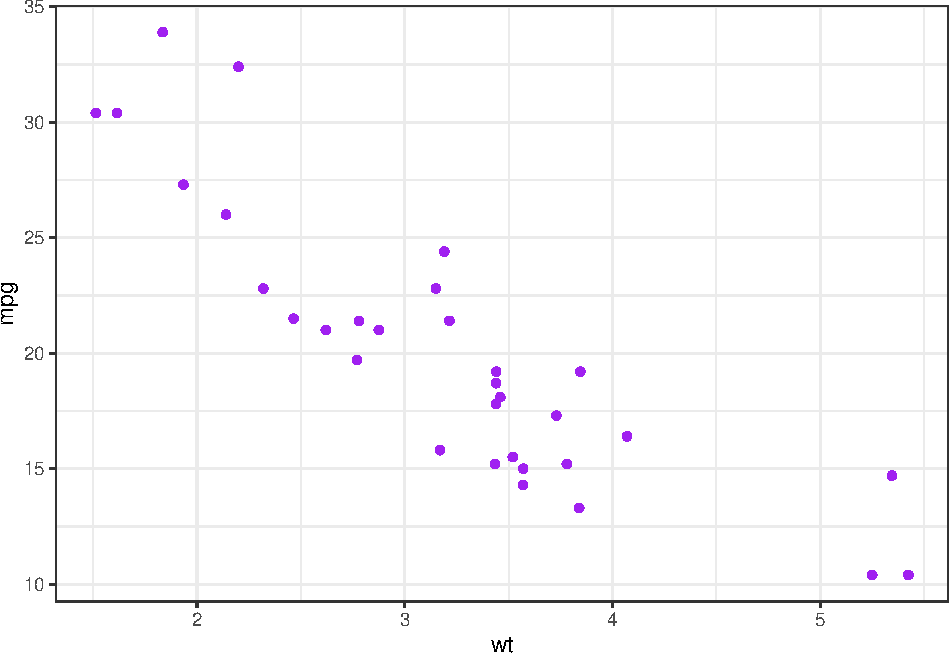
\includegraphics{Introduccion_a_Muestreo_files/figure-latex/unnamed-chunk-98-1.pdf}
Para obtener toda la matriz de correlaciones de la base podemos tomar \texttt{cor} aplicado a toda la base de datos:

\begin{Shaded}
\begin{Highlighting}[]
\FunctionTok{cor}\NormalTok{(datos.coches, }\AttributeTok{method =} \StringTok{"pearson"}\NormalTok{)}
\end{Highlighting}
\end{Shaded}

\begin{verbatim}
##             mpg        cyl       disp         hp        drat         wt
## mpg   1.0000000 -0.8521620 -0.8475514 -0.7761684  0.68117191 -0.8676594
## cyl  -0.8521620  1.0000000  0.9020329  0.8324475 -0.69993811  0.7824958
## disp -0.8475514  0.9020329  1.0000000  0.7909486 -0.71021393  0.8879799
## hp   -0.7761684  0.8324475  0.7909486  1.0000000 -0.44875912  0.6587479
## drat  0.6811719 -0.6999381 -0.7102139 -0.4487591  1.00000000 -0.7124406
## wt   -0.8676594  0.7824958  0.8879799  0.6587479 -0.71244065  1.0000000
## qsec  0.4186840 -0.5912421 -0.4336979 -0.7082234  0.09120476 -0.1747159
## vs    0.6640389 -0.8108118 -0.7104159 -0.7230967  0.44027846 -0.5549157
## am    0.5998324 -0.5226070 -0.5912270 -0.2432043  0.71271113 -0.6924953
## gear  0.4802848 -0.4926866 -0.5555692 -0.1257043  0.69961013 -0.5832870
## carb -0.5509251  0.5269883  0.3949769  0.7498125 -0.09078980  0.4276059
##             qsec         vs          am       gear        carb
## mpg   0.41868403  0.6640389  0.59983243  0.4802848 -0.55092507
## cyl  -0.59124207 -0.8108118 -0.52260705 -0.4926866  0.52698829
## disp -0.43369788 -0.7104159 -0.59122704 -0.5555692  0.39497686
## hp   -0.70822339 -0.7230967 -0.24320426 -0.1257043  0.74981247
## drat  0.09120476  0.4402785  0.71271113  0.6996101 -0.09078980
## wt   -0.17471588 -0.5549157 -0.69249526 -0.5832870  0.42760594
## qsec  1.00000000  0.7445354 -0.22986086 -0.2126822 -0.65624923
## vs    0.74453544  1.0000000  0.16834512  0.2060233 -0.56960714
## am   -0.22986086  0.1683451  1.00000000  0.7940588  0.05753435
## gear -0.21268223  0.2060233  0.79405876  1.0000000  0.27407284
## carb -0.65624923 -0.5696071  0.05753435  0.2740728  1.00000000
\end{verbatim}

Finalmente, el paquete \texttt{ggcorrplot} puede ayudarnos a visualizar gráficamente dicha matriz:

\begin{Shaded}
\begin{Highlighting}[]
\FunctionTok{ggcorrplot}\NormalTok{(}\FunctionTok{cor}\NormalTok{(datos.coches, }\AttributeTok{method =} \StringTok{"pearson"}\NormalTok{), }
           \AttributeTok{lab =} \ConstantTok{TRUE}\NormalTok{,}
           \AttributeTok{type =} \StringTok{"upper"}\NormalTok{) }\SpecialCharTok{+}
  \FunctionTok{labs}\NormalTok{(}\AttributeTok{title =} \StringTok{"Matriz de Correlaciones"}\NormalTok{)}
\end{Highlighting}
\end{Shaded}

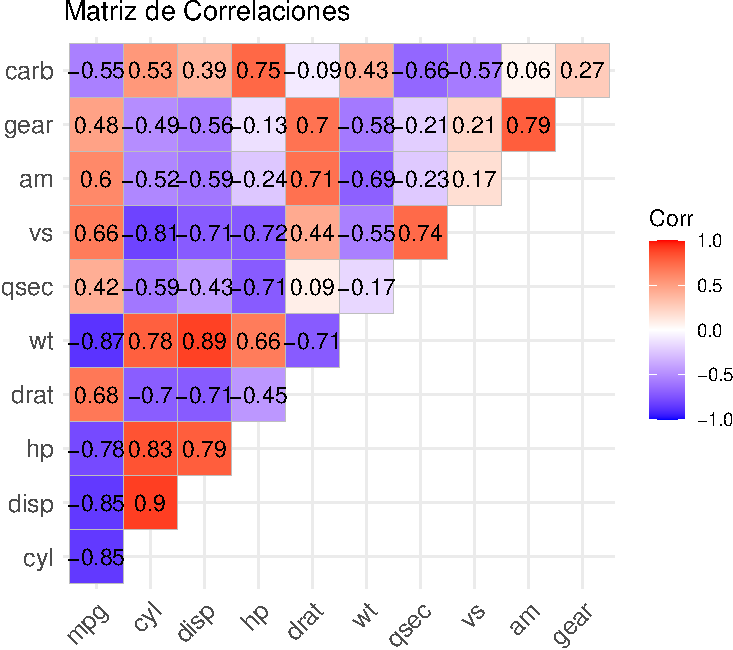
\includegraphics{Introduccion_a_Muestreo_files/figure-latex/unnamed-chunk-100-1.pdf}

\begin{quote}
Una correlación de Pearson igual a \(1\) ó \(-1\) se interpreta como que hay una relación lineal perfecta mientras que una correlación igual a \(0\) se interpreta como que no hay relación lineal (aunque puede existir de otro tipo)
\end{quote}

\begin{Shaded}
\begin{Highlighting}[]
\CommentTok{\#Ejemplo de correlación lineal perfecta}
\NormalTok{x }\OtherTok{\textless{}{-}} \FunctionTok{seq}\NormalTok{(}\DecValTok{0}\NormalTok{,}\DecValTok{4}\NormalTok{, }\AttributeTok{length.out =} \DecValTok{9}\NormalTok{)}
\NormalTok{y }\OtherTok{\textless{}{-}} \DecValTok{2}\SpecialCharTok{*}\NormalTok{x }\SpecialCharTok{+} \DecValTok{1}
\end{Highlighting}
\end{Shaded}

Gráficamente:

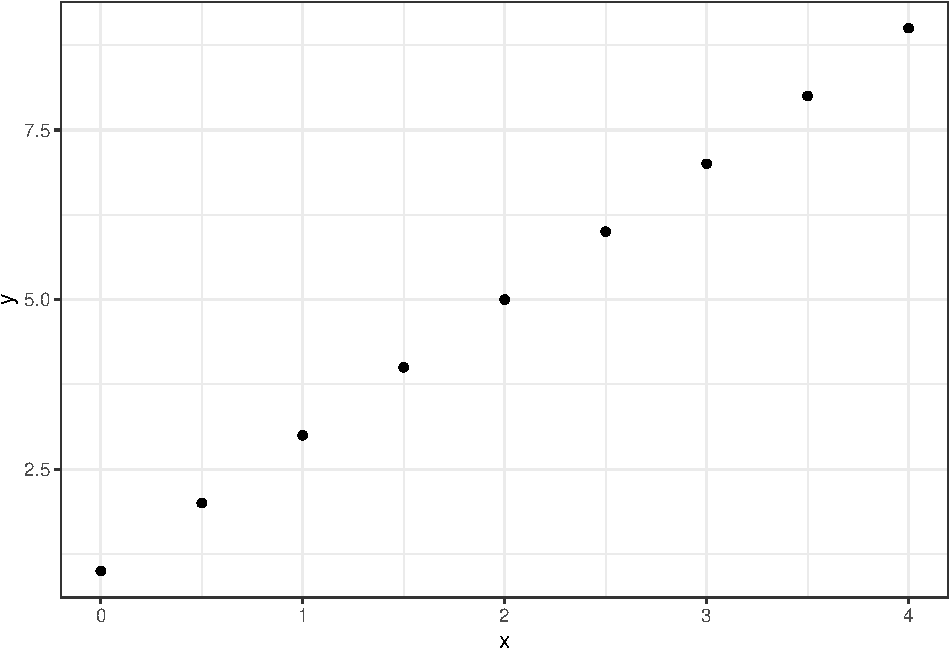
\includegraphics{Introduccion_a_Muestreo_files/figure-latex/unnamed-chunk-102-1.pdf}

El valor en este caso de la correlación es:

\begin{Shaded}
\begin{Highlighting}[]
\FunctionTok{cor}\NormalTok{(x,y, }\AttributeTok{method =} \StringTok{"pearson"}\NormalTok{)}
\end{Highlighting}
\end{Shaded}

\begin{verbatim}
## [1] 1
\end{verbatim}

Mientras que por otro lado podemos tener variables relacionadas pero \emph{sin correlación} :

\begin{Shaded}
\begin{Highlighting}[]
\CommentTok{\#Ejemplo sin correlación lineal pero con variables relacionadas}
\NormalTok{x }\OtherTok{\textless{}{-}} \FunctionTok{seq}\NormalTok{(}\SpecialCharTok{{-}}\DecValTok{4}\NormalTok{, }\DecValTok{4}\NormalTok{,}\AttributeTok{length.out =} \DecValTok{9}\NormalTok{)}
\NormalTok{y }\OtherTok{\textless{}{-}}\NormalTok{ x}\SpecialCharTok{\^{}}\DecValTok{2}
\FunctionTok{cor}\NormalTok{(x,y, }\AttributeTok{method =} \StringTok{"pearson"}\NormalTok{)}
\end{Highlighting}
\end{Shaded}

\begin{verbatim}
## [1] 0
\end{verbatim}

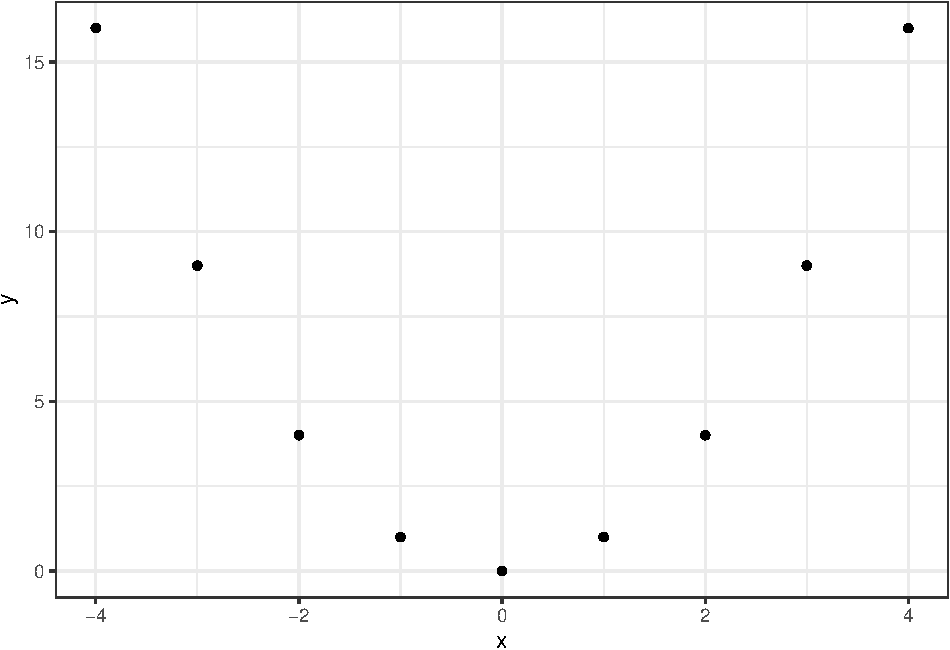
\includegraphics{Introduccion_a_Muestreo_files/figure-latex/unnamed-chunk-105-1.pdf}

\textbf{6. Correlación de rango de Spearman} Para hablar de la correlación de rango de Spearman es necesario definir una variable como \textbf{ordinal}.

Un vector \(\vec{x} = (x_1, x_2, \dots, x_n)^T\) de variables numéricas o categóricas es \textbf{ordinal} si existe una relación \(\leq\) de \href{https://en.wikipedia.org/wiki/Total_order}{orden total} sobre los elementos del vector tal que:

\begin{enumerate}
\def\labelenumi{\arabic{enumi}.}
\item
  Es \emph{antisimétrica}: si \(x_i \leq x_j\) y \(x_j \leq x_i\) entonces \(x_i = x_j\).
\item
  Es \emph{transitiva}: si \(x_i \leq x_j\) y \(x_j \leq x_k\) entonces \(x_i \leq x_k\).
\item
  Es \emph{conexa}: \(x_i \leq x_j\) ó \(x_j \leq x_i\).
\end{enumerate}

De manera intuitiva un vector es \textbf{ordinal} si hay un orden para sus entradas. Por ejemplo, cuando calificas un servicio como \texttt{Malo} \(\leq\) \texttt{Regular} \(\leq\) \texttt{Bueno} o bien cuando se compara nivel educativo (en términos de años) \texttt{Primaria} \(\leq\) \texttt{Secundaria} \(\leq\) \texttt{Preparatoria} \(\leq\) \texttt{Educación\ superior}. \textbf{Toda variable numérica es ordinal}.

Para un vector ordinal definimos su ordenamiento como \(x_{(1)} = \min \{ x_1, x_2, \dots, x_n \}\) y \(x_{(j)} = \min \{ x_1, x_2, \dots, x_n \} \setminus \{ x_{(1)}, x_{(2)}, \dots, x_{(j-1)} \}\) de tal forma que \(x_{(1)} \leq x_{(2)} \leq \dots \leq x_{(n)}\). El rango de \(x_{(j)}\) denotado como \(R(x_{(j)})\) es \(j\) (su posición en el ordenamiento). Es decir:
\[
R(x_i) = j \Leftrightarrow x_i = x_{(j)}
\]

Dado un vector \(\vec{x}\) definimos su \textbf{vector de rango} como:

\[
R(\vec{x}) = \big( R(x_1), R(x_2), \dots, R(x_n) )^T
\]

Para dos variables ordinales, \(\vec{x}\) y \(\vec{y}\) se define la \textbf{correlación de rango de Spearman} como la correlación de Pearson entre sus vectores de rangos:

\[
\rho_{\text{Spearman}} =\rho\big( R(\vec{x}), R(\vec{y}))
\]

\begin{quote}
Mientras que la correlación de Pearson mide linealidad; la de Spearman mide monotonicidad (que si una aumenta la otra también; que si una disminuye la otra también).
\end{quote}

\begin{Shaded}
\begin{Highlighting}[]
\CommentTok{\#Comparativo de correlaciones: la de Pearson no encuentra mucha línea}
\NormalTok{x }\OtherTok{\textless{}{-}} \FunctionTok{seq}\NormalTok{(}\FloatTok{0.1}\NormalTok{, }\DecValTok{1}\NormalTok{, }\AttributeTok{length.out =} \DecValTok{25}\NormalTok{)}
\NormalTok{y }\OtherTok{\textless{}{-}} \FunctionTok{exp}\NormalTok{(}\DecValTok{1}\SpecialCharTok{/}\NormalTok{x}\SpecialCharTok{\^{}}\DecValTok{2}\NormalTok{)}
\end{Highlighting}
\end{Shaded}

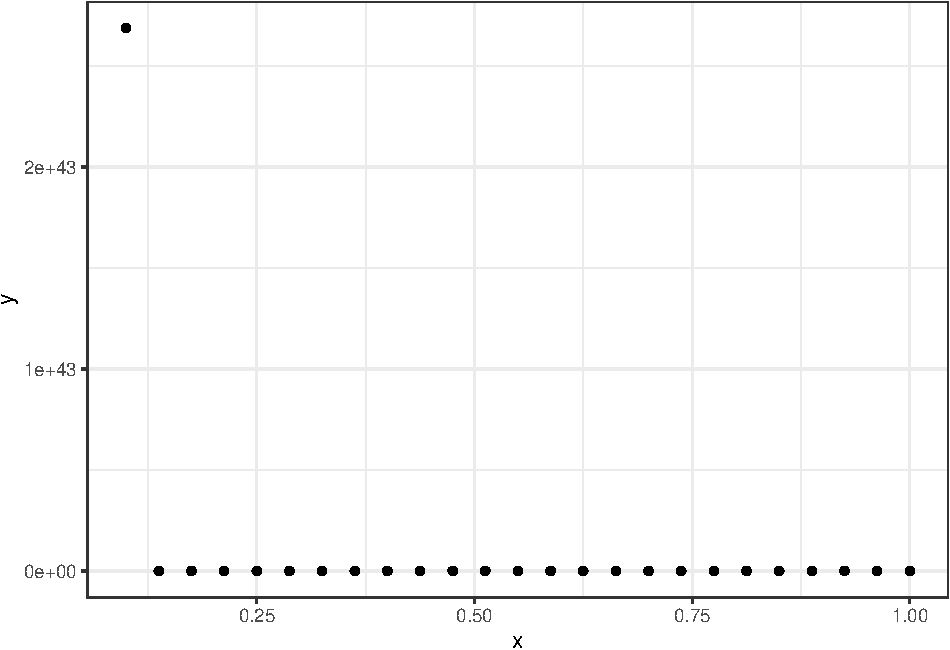
\includegraphics{Introduccion_a_Muestreo_files/figure-latex/unnamed-chunk-107-1.pdf}

En este caso la correlación de Pearson es muy mala:

\begin{Shaded}
\begin{Highlighting}[]
\FunctionTok{cor}\NormalTok{(x,y, }\AttributeTok{method =} \StringTok{"pearson"}\NormalTok{)}
\end{Highlighting}
\end{Shaded}

\begin{verbatim}
## [1] -0.3396831
\end{verbatim}

Mientras que la de Spearman sí muestra la relación:

\begin{Shaded}
\begin{Highlighting}[]
\FunctionTok{cor}\NormalTok{(x,y, }\AttributeTok{method =} \StringTok{"spearman"}\NormalTok{)}
\end{Highlighting}
\end{Shaded}

\begin{verbatim}
## [1] -1
\end{verbatim}

\textbf{7. \(\tau\) de Kendall} Consideremos \(\vec{x}\) y \(\vec{y}\) dos vectores columna ordinales de una matriz de datos \(Z\). Para cualquier par de observaciones \((x_i, y_i)\) y \((x_j, y_j)\) con \(i < j\) decimos que dos observaciones son \textbf{concordantes (\(c\))} si los rangos de ambas \(x\) y \(y\) coinciden; es decir si se cumple una de las siguientes:

\begin{enumerate}
\def\labelenumi{\arabic{enumi}.}
\item
  \(R(x_i) < R(x_j)\) y \(R(y_i) < R(y_j)\) o bien,
\item
  \(R(x_i) > R(x_j)\) y \(R(y_i) > R(y_j)\).
\end{enumerate}

Observaciones \textbf{discordantes (\(d\))} ocurren cuando los rangos de las \(x\) y las \(y\) son inversos el uno del otro; es decir, se cumple una de las siguientes:

\begin{enumerate}
\def\labelenumi{\arabic{enumi}.}
\item
  \(R(x_i) > R(x_j)\) y \(R(y_i) < R(y_j)\) o bien,
\item
  \(R(x_i) < R(x_j)\) y \(R(y_i) > R(y_j)\).
\end{enumerate}

En el caso que cualquiera de las dos, \(x\) ó \(y\) sean igualdades (\(x_i = x_j\) ó \(y_i = y_j\)) no son discordantes ni concordantes.

Observa que existen \(\binom{n}{2}\) distintos pares de \((x_i,y_i)\) y \((x_j,y_j)\) para comparar. Sea \(c_{\vec{x},\vec{y}}\) la cantidad de pares concordantes y \(d_{\vec{x},\vec{y}}\) la cantidad de pares discordantes. Luego la probabilidad de que dos pares seleccionados de manera uniforme sean concordantes es:
\[
\dfrac{c_{\vec{x},\vec{y}}}{\binom{n}{2}}
\]
mientras que la probabilidad de que dos pares seleccionados uniformemente sean discordantes es:
\[
\dfrac{d_{\vec{x},\vec{y}}}{\binom{n}{2}}.
\]

Definimos entonces la \(\tau\) de Kendall como la diferencia entre ambas probabilidades empíricas:
\[
\tau_{\vec{x},\vec{y}} = \dfrac{c_{\vec{x},\vec{y}} - d_{\vec{x},\vec{y}}}{\binom{n}{2}}
\]
La tau de Kendall cumple que:
\[
-1 \leq \tau_{\vec{x},\vec{y}} \leq 1
\]
donde el \(-1\) se alcanza sólo si son completamente discordantes (el rango de \(x\) es el inverso del rango de las \(y\)) y el \(1\) si son completamente concordantes (el rango de \(x\) y de \(y\) tienen el mismo orden). Una \(\tau\) cercana a cero se interpreta como ausencia de relación en los rangos.

Podemos aplicar la tau de Kendall a la siguiente base de datos que contiene la calificación de dos servicios de un restaurante:

\begin{table}
\centering
\begin{tabular}{l|l}
\hline
calidad\_alimentos & calidad\_servicio\\
\hline
\cellcolor{gray!6}{Malo} & \cellcolor{gray!6}{1 estrella}\\
\hline
Bueno & 4 \vphantom{1} estrellas\\
\hline
\cellcolor{gray!6}{Bueno} & \cellcolor{gray!6}{5 \vphantom{1} estrellas}\\
\hline
Regular & 2 estrellas\\
\hline
\cellcolor{gray!6}{Bueno} & \cellcolor{gray!6}{5 estrellas}\\
\hline
Bueno & 4 estrellas\\
\hline
\end{tabular}
\end{table}

Para ello codificamos las variables como \texttt{factor} diciéndole que son variables ordinales \texttt{order\ =\ TRUE} e indicando el orden de los niveles:

\begin{Shaded}
\begin{Highlighting}[]
\NormalTok{calidad\_alimentos }\OtherTok{\textless{}{-}} \FunctionTok{factor}\NormalTok{(}\FunctionTok{c}\NormalTok{(}\StringTok{"Malo"}\NormalTok{,}\StringTok{"Bueno"}\NormalTok{,}\StringTok{"Bueno"}\NormalTok{,}\StringTok{"Regular"}\NormalTok{,}\StringTok{"Bueno"}\NormalTok{,}\StringTok{"Bueno"}\NormalTok{),}
                            \AttributeTok{order =} \ConstantTok{TRUE}\NormalTok{, }
                            \AttributeTok{levels =} \FunctionTok{c}\NormalTok{(}\StringTok{"Malo"}\NormalTok{,}\StringTok{"Regular"}\NormalTok{,}\StringTok{"Bueno"}\NormalTok{))}
\NormalTok{calidad\_servicio }\OtherTok{\textless{}{-}} \FunctionTok{factor}\NormalTok{(}\FunctionTok{c}\NormalTok{(}\StringTok{"1 estrella"}\NormalTok{, }\StringTok{"4 estrellas"}\NormalTok{,  }\StringTok{"5 estrellas"}\NormalTok{, }
                             \StringTok{"2 estrellas"}\NormalTok{, }\StringTok{"5 estrellas"}\NormalTok{,}\StringTok{"4 estrellas"}\NormalTok{),}
                            \AttributeTok{order =} \ConstantTok{TRUE}\NormalTok{, }
                            \AttributeTok{levels =} \FunctionTok{c}\NormalTok{(}\StringTok{"1 estrella"}\NormalTok{,}\StringTok{"2 estrellas"}\NormalTok{,}\StringTok{"3 estrellas"}\NormalTok{,}
                                       \StringTok{"4 estrellas"}\NormalTok{,}\StringTok{"5 estrellas"}\NormalTok{))}
\end{Highlighting}
\end{Shaded}

Esto de las variables ordinales permite hacer comparaciones ordinales, por ejemplo:

\begin{Shaded}
\begin{Highlighting}[]
\NormalTok{calidad\_alimentos[}\DecValTok{2}\NormalTok{] }\SpecialCharTok{\textgreater{}}\NormalTok{ calidad\_alimentos[}\DecValTok{4}\NormalTok{]}
\end{Highlighting}
\end{Shaded}

\begin{verbatim}
## [1] TRUE
\end{verbatim}

Los datos se ven así:

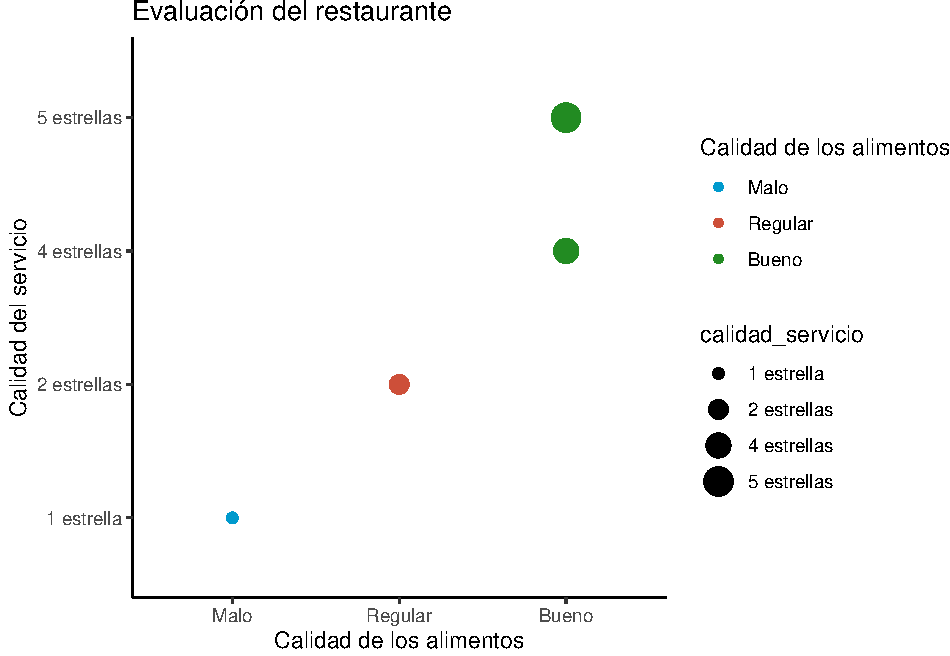
\includegraphics{Introduccion_a_Muestreo_files/figure-latex/unnamed-chunk-113-1.pdf}

Finalmente, calculamos la \(\tau\) de Kendall, para ello es necesario obtener el rango de nuestras variables ordinales:

\begin{Shaded}
\begin{Highlighting}[]
\NormalTok{rango\_alimentos }\OtherTok{\textless{}{-}} \FunctionTok{as.numeric}\NormalTok{(calidad\_alimentos)}
\NormalTok{rango\_servicio  }\OtherTok{\textless{}{-}} \FunctionTok{as.numeric}\NormalTok{(calidad\_servicio)}
\FunctionTok{cor}\NormalTok{(rango\_alimentos, rango\_servicio, }\AttributeTok{method =} \StringTok{"kendall"}\NormalTok{)}
\end{Highlighting}
\end{Shaded}

\begin{verbatim}
## [1] 0.8320503
\end{verbatim}

Lo cual indica que hay una relación entre la calificación de calidad de alimentos y la del servicio.

\textbf{8. Ajuste de modelo lineal}

Sean \(\vec{x}\) y \(\vec{y}\) dos vectores columna de una matriz de datos \(Z\). Supongamos, además, se tiene la hipótesis de que existe una relación afín entre los vectores; es decir que:
\[
\vec{y} \approx \beta_1 \vec{x} + \beta_0 \vec{1} 
\]
donde \(\vec{1} = (1, 1, \dots, 1)^T\) es un vector con todas las entradas idénticas a \(1\) y \(\beta_0, \beta_1 \in \mathbb{R}\). Algunas razónes para tener esta hipótesis podría ser una correlación de Pearson cercana a \(\pm 1\) o por inspección gráfica. Esta hipótesis implica que:
\[
y \approx \underbrace{\beta_1 x + \beta_0}_{\hat{y}}
\]
Podemos entonces trazar la línea \(y = \beta_0 + \beta_1 x\) y graficar contra los puntos \(\{(x_i,y_i)\}_{i=1}^{n}\), Si la línea no ajusta perfecto tendremos errores \(e_i = (y_i - \hat{y}_i)^2\) de predicción las cuales representan la diferencia entre la \(y\) observada (\(y_i\)) y la \(y\) predicha por la línea \(\hat{y}_i = \beta_1 x_i + \beta_0\). La suma de estos errores es:
\[
\textrm{SSR}(\beta_0, \beta_1) = \sum\limits_{i=1}^{n} e_i = \sum\limits_{i=1}^{n} \big( y_i - \hat{y}_i \big)^2 = \sum\limits_{i=1}^{n} \big( y_i - (\beta_1 x_i + \beta_0) \big)^2 
\]

El nombre de \emph{SSR} es por ( \emph{Sum of Squared Residuals} ) dado que en estadística se define un residual como \(r_i = (y_i - \hat{y}_i)\)
Gráficamente:

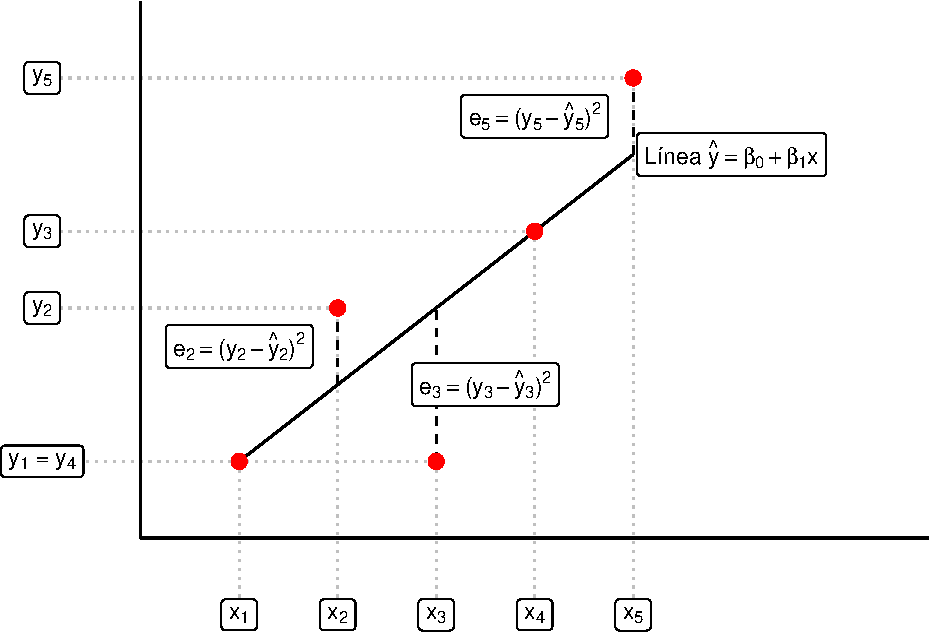
\includegraphics{Introduccion_a_Muestreo_files/figure-latex/unnamed-chunk-115-1.pdf}

Lo que se busca entonces es minimizar el error respecto a las constantes a determinar: \(\beta_0\) y \(\beta_1\). Para ello buscamos un punto de inflexión derivando:
\[
\dfrac{\partial\textrm{SSR}}{\partial \beta_0} = \sum\limits_{i=1}^{n} 2\big(y_i - (\beta_1 x_i + \beta_0 ) \big) = 0
\]

De donde se sigue que:
\[
\sum\limits_{i=1}^n y_i - \beta_1 \sum\limits_{i=1}^{n} x_i - n \beta_0 = 0 \Rightarrow \beta_0 = \dfrac{1}{n} \sum\limits_{i=1}^n y_i - \beta_1 \dfrac{1}{n} \sum\limits_{i=1}^n x_i \Rightarrow \bar{y} - \beta_1 \bar{x},
\]

de donde concluimos que de cumplirse la relación lineal se tiene que:
\[
\beta_0 = \bar{y} - \beta_1 \bar{x}.
\]

Por otro lado, la derivada respecto a \(\beta_1\) es:
\[
\dfrac{\partial\textrm{SSR}}{\partial \beta_1} = - \sum\limits_{i=1}^{n} 2\big(y_i - (\beta_1 x_i + \beta_0 ) \big) \cdot x_i = 0
\]

De donde se sigue (si suponemos que existe al menos un \(x_i \neq 0\)):
\begin{equation}\nonumber
\begin{aligned}
0 & = - \sum\limits_{i=1}^n \Big( x_i y_i - \beta_1  x_i^2 - \underbrace{\beta_0}_{\bar{y} - \beta_1 \bar{x}} x_i \Big)  \\
& = \sum\limits_{i=1}^n \Big( x_i y_i - \beta_1  x_i^2 - \bar{y}x_i + \beta_1 \bar{x} x_i \Big) \\
& = \sum\limits_{i=1}^n \Big( y_i + \beta_1  x_i - \bar{y} - \beta_1 \bar{x} \Big) x_i \\
& = \sum\limits_{i=1}^n \Big( y_i  - \bar{y} \Big) x_i - \beta_1  \sum\limits_{i=1}^n\Big(   x_i -   \bar{x} \Big) x_i
\end{aligned}
\end{equation}
de donde se sigue (suponiendo que existen \(i,j\) tales que \(x_i \neq x_j\) que:
\[
\beta_1 = \dfrac{\sum_{i=1}^n \Big( y_i  - \bar{y} \Big)x_i}{\sum_{i=1}^n\Big(   x_i -   \bar{x} \Big)x_i} = \dfrac{\sum_{i=1}^n \Big( y_i  - \bar{y} \Big)\Big(   x_i -   \bar{x} \Big)}{\sum_{i=1}^n\Big(   x_i -   \bar{x} \Big)^2} = \dfrac{\sigma_{\vec{x}} \cdot \sigma_{\vec{y}} \cdot \rho_{\vec{x},\vec{y}}}{n \sigma_{\vec{x}}^2}
\]
por lo cual:
\[
\beta_1 = \dfrac{\sigma_{\vec{y}}}{\sigma_{\vec{x}}} \cdot \dfrac{\rho_{\vec{x},\vec{y}}}{n}
\]

De donde se tienen las fórmulas para el \(\beta_0\) y \(\beta_1\).

\hypertarget{ejercicio-2}{%
\subsection{Ejercicio}\label{ejercicio-2}}

Demuestra la igualdad que usamos anteriormente:

\[
\dfrac{\sum_{i=1}^n \Big( y_i  - \bar{y} \Big) x_i}{\sum_{i=1}^n\Big(   x_i -   \bar{x} \Big)x_i} = \dfrac{\sum_{i=1}^n \Big( y_i  - \bar{y} \Big)\Big(   x_i -   \bar{x} \Big)}{\sum_{i=1}^n\Big(   x_i -   \bar{x} \Big)^2} 
\]

En \texttt{R} podemos ajustar un modelo lineal para dos variables de una base de datos con \texttt{lm}:

\begin{Shaded}
\begin{Highlighting}[]
\NormalTok{modelo.lineal }\OtherTok{\textless{}{-}} \FunctionTok{lm}\NormalTok{(mpg }\SpecialCharTok{\textasciitilde{}}\NormalTok{ wt, }\AttributeTok{data =}\NormalTok{ datos.coches)}
\FunctionTok{coef}\NormalTok{(modelo.lineal)}
\end{Highlighting}
\end{Shaded}

\begin{verbatim}
## (Intercept)          wt 
##   37.285126   -5.344472
\end{verbatim}

Gráficamente podemos ver el modelo:

\begin{Shaded}
\begin{Highlighting}[]
\FunctionTok{ggplot}\NormalTok{(datos.coches) }\SpecialCharTok{+}
  \FunctionTok{geom\_point}\NormalTok{(}\FunctionTok{aes}\NormalTok{(}\AttributeTok{y =}\NormalTok{ mpg, }\AttributeTok{x =}\NormalTok{ wt)) }\SpecialCharTok{+}
  \FunctionTok{geom\_smooth}\NormalTok{(}\FunctionTok{aes}\NormalTok{(}\AttributeTok{y =}\NormalTok{ mpg, }\AttributeTok{x =}\NormalTok{ wt), }\AttributeTok{method =} \StringTok{"lm"}\NormalTok{, }
              \AttributeTok{formula =}\NormalTok{ y }\SpecialCharTok{\textasciitilde{}}\NormalTok{ x, }\AttributeTok{se =} \ConstantTok{FALSE}\NormalTok{) }\SpecialCharTok{+}
  \FunctionTok{theme\_minimal}\NormalTok{()}
\end{Highlighting}
\end{Shaded}

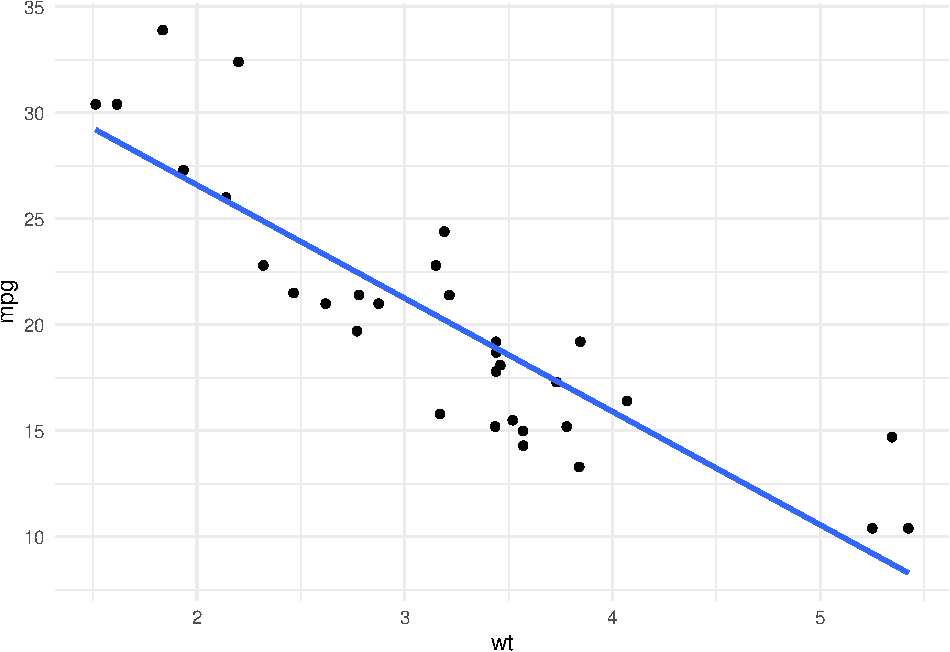
\includegraphics{Introduccion_a_Muestreo_files/figure-latex/unnamed-chunk-117-1.pdf}

Para predecir, dada una nueva observación, cuál debe haber sido el valor de \(\hat{y}\) para una nueva observación \(x_*\) (o varias nuevas observaciones) puede usarse la función \texttt{predict}

\begin{Shaded}
\begin{Highlighting}[]
\NormalTok{datos\_a\_predecir }\OtherTok{\textless{}{-}} \FunctionTok{data.frame}\NormalTok{(}\AttributeTok{wt =} \FunctionTok{c}\NormalTok{(}\FloatTok{5.5}\NormalTok{, }\DecValTok{6}\NormalTok{, }\FloatTok{6.5}\NormalTok{))}
\FunctionTok{predict}\NormalTok{(modelo.lineal, datos\_a\_predecir)}
\end{Highlighting}
\end{Shaded}

\begin{verbatim}
##        1        2        3 
## 7.890533 5.218297 2.546061
\end{verbatim}

Hay que tener mucho cuidado con la generalización de un modelo lineal como los siguientes valores muestran:

\begin{Shaded}
\begin{Highlighting}[]
\NormalTok{datos\_a\_predecir }\OtherTok{\textless{}{-}} \FunctionTok{data.frame}\NormalTok{(}\AttributeTok{wt =} \FunctionTok{c}\NormalTok{(}\DecValTok{7}\NormalTok{,}\DecValTok{8}\NormalTok{,}\DecValTok{9}\NormalTok{))}
\FunctionTok{predict}\NormalTok{(modelo.lineal, datos\_a\_predecir)}
\end{Highlighting}
\end{Shaded}

\begin{verbatim}
##           1           2           3 
##  -0.1261748  -5.4706464 -10.8151180
\end{verbatim}

O bien el siguiente \href{https://xkcd.com/605/}{comic de xkcd}:

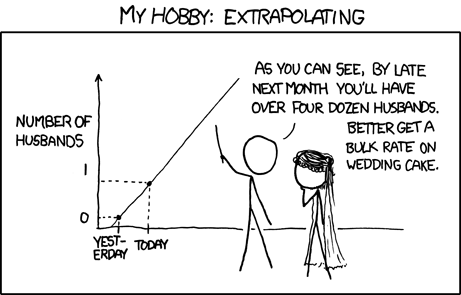
\includegraphics[width=6.4in]{images/extrapolating}

Para hacer la extrapolación gráfica podemos agregar un \texttt{fullrange\ =\ TRUE} combinado con un \texttt{xlim}

\begin{Shaded}
\begin{Highlighting}[]
\FunctionTok{ggplot}\NormalTok{(datos.coches) }\SpecialCharTok{+}
  \FunctionTok{geom\_point}\NormalTok{(}\FunctionTok{aes}\NormalTok{(}\AttributeTok{y =}\NormalTok{ mpg, }\AttributeTok{x =}\NormalTok{ wt)) }\SpecialCharTok{+}
  \FunctionTok{geom\_smooth}\NormalTok{(}\FunctionTok{aes}\NormalTok{(}\AttributeTok{y =}\NormalTok{ mpg, }\AttributeTok{x =}\NormalTok{ wt), }\AttributeTok{method =} \StringTok{"lm"}\NormalTok{, }
              \AttributeTok{formula =}\NormalTok{ y }\SpecialCharTok{\textasciitilde{}}\NormalTok{ x, }\AttributeTok{se =} \ConstantTok{FALSE}\NormalTok{, }\AttributeTok{fullrange=}\ConstantTok{TRUE}\NormalTok{) }\SpecialCharTok{+}
  \FunctionTok{theme\_minimal}\NormalTok{() }\SpecialCharTok{+}
  \FunctionTok{xlim}\NormalTok{(}\FunctionTok{c}\NormalTok{(}\DecValTok{1}\NormalTok{,}\FloatTok{6.5}\NormalTok{))}
\end{Highlighting}
\end{Shaded}

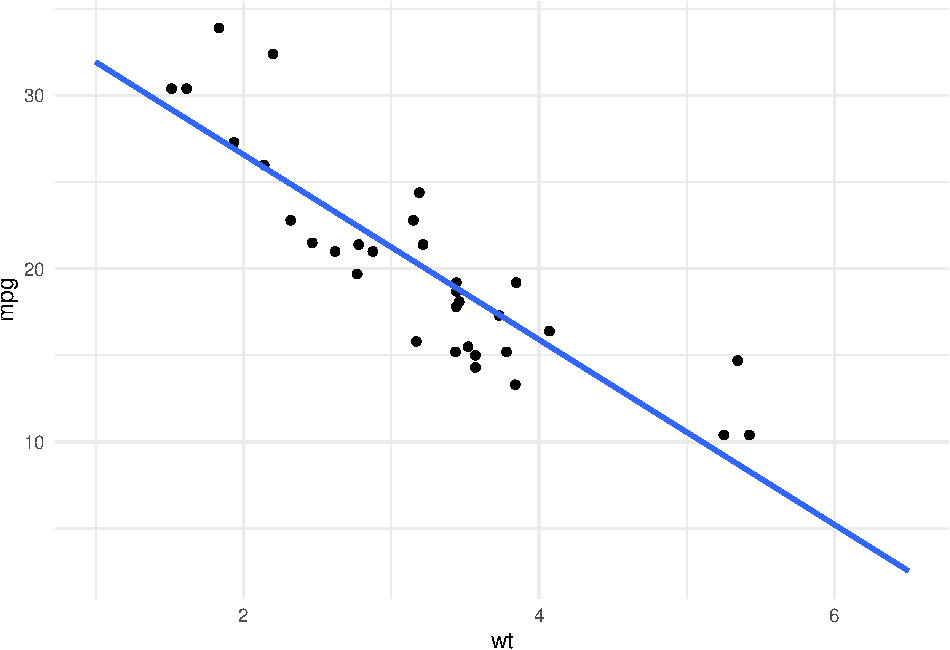
\includegraphics{Introduccion_a_Muestreo_files/figure-latex/unnamed-chunk-121-1.pdf}

\hypertarget{ejercicio-3}{%
\section{Ejercicio}\label{ejercicio-3}}

\begin{enumerate}
\def\labelenumi{\arabic{enumi}.}
\tightlist
\item
  Generaliza el proceso de estimación para cuando se tiene un polinomio \(y = \beta_0 + \beta_1 x + \beta_2 x^2\)
\item
  Utiliza los datos confirmados de COVID-19 a nivel nacional (sólo los confirmados) disponibles en \href{https://datos.gob.mx/busca/dataset/informacion-referente-a-casos-covid-19-en-mexico}{este link}. Ajusta un modelo cuadrático (en el \texttt{lm} la fórmula ahora es del estilo de \texttt{y\ \textasciitilde{}\ poly(x,2)} ) y predice cuántos casos confirmados habrá el 29 de junio. Grafica tu ajuste así como tu predicción en la misma gráfica.
\end{enumerate}

\textbf{9. Ajuste general}
Podemos generalizar el ajuste de mínimos cuadrados planteando el modelo \(y = f(x, \vec{\beta})\) donde \(x\) puede ser una matriz y \(\vec{\beta}\) es un vector de parámetros. Supondremos que \(f\) es diferenciable en \(\vec{\beta}\).

Como ejemplo, en el caso del ajuste lineal:
\[
y = f(x, \vec{\beta}) = \beta_0 + \beta_1 x \qquad \text{con} \qquad \vec{\beta}= (\beta_0,\beta_1)^T.
\]
o bien podríamos pensar en un ajuste polinomial:
\[
y = f(x, \vec{\beta}) = \sum\limits_{i = 0}^n \beta_i x^i \qquad \text{con} \qquad \vec{\beta}= (\beta_0,\beta_1, \dots, \beta_n)^T.
\]
No tiene que ser un polinomio, \(f\) puede ser lo que ella quiera ser siempre y cuando sea diferenciable en los parámetros:
\[
y = f(x, \vec{\beta}) = \Bigg[\cos(\beta_0 + x) + \int\limits_{0}^{\beta_1 x} e^{-t^2} dx \Bigg] \cdot \beta_2 \ln(x) \qquad \text{con} \qquad \vec{\beta}= (\beta_0,\beta_1, \beta_3)^T.
\]

\hypertarget{ajuste-funcional}{%
\section{Ajuste funcional}\label{ajuste-funcional}}

Hacemos una apuesta por teléfono. Yo voy a tirar una moneda \(10\) veces y si salen más \texttt{Soles} que \texttt{Águilas} yo gano 50 pesos. Si salen más \texttt{Águilas} que \texttt{Soles} tú ganas la misma cantidad. Al realizar el ejercicio yo te comunico que salieron en total \(10\) \texttt{Soles} y por tanto me debes el dinero. \emph{¿Sospecharías algo de mí?}

Si no hablamos de probabilidad no hay forma en la que se pueda justificar que \emph{aparentemente} hay algo raro con la moneda. Claro, siempre puede ser un caso improbable (\href{https://www.youtube.com/watch?v=rwvIGNXY21Y}{hay gente que lo ha hecho}) pero es \emph{raro} que me hayan salido tantos \texttt{Soles}. Para cuantificar qué tan raro es el evento podemos suponer que las monedas siguen un modelo Binomial con parámetro \(p = 1/2\) y en este caso \(n = 10\) (fueron 10 tiros). La probabilidad de que haya obtenido \(10\) soles bajo este modelo es de:

\begin{Shaded}
\begin{Highlighting}[]
\FunctionTok{dbinom}\NormalTok{(}\DecValTok{10}\NormalTok{,}\DecValTok{10}\NormalTok{, }\DecValTok{1}\SpecialCharTok{/}\DecValTok{2}\NormalTok{)}
\end{Highlighting}
\end{Shaded}

\begin{verbatim}
## [1] 0.0009765625
\end{verbatim}

¡Rarísimo! Este resultado te haría sospechar que quizá mi moneda no es \emph{justa} y no se obtienen la misma cantidad de \texttt{Águilas} que \texttt{Soles} cuando la tiro. Esto porque, aparentemente, en mi moneda la probabilidad de \texttt{Sol} debería de ser \(p = 1\) (por tu triste experiencia). Si por ejemplo en el onceavo tiro saliera un \texttt{Águila}, concluirías que, en mi moneda, aparentemente, la probabilidad de \texttt{Sol} es \(p = \frac{10}{11}\). Por supuesto, entre más tiros y más información obtienes, mejor podrás caracterizar la moneda y con mayor sustento tendrás sospechas (o no) de que mi moneda es tramposa.

Formalmente, en el ejemplo anterior, lo que se hace es suponer que existe una variable aleatoria \(X \in\{ \text{Águila}, \text{Sol}\}\) (el resultado de la moneda) de la cual observamos \(n = 11\) realizaciones codificadas en el siguiente vector:

\[
\vec{x} = \big( \text{Sol}, \text{Sol},\text{Sol},\text{Sol},\text{Sol},\text{Sol},\text{Sol},\text{Sol},\text{Sol},\text{Sol},\text{Águila}\big)^T
\]

Aproximamos entonces la probabilidad \(\mathbb{P}(X = \text{Sol})\) mediante:

\[
\mathbb{P}(X = \text{Sol}) \approx \dfrac{1}{n}\sum\limits_{i=1}^n \mathbb{I}_{\{\text{Sol}\}}(x_i) = \dfrac{10}{11}
\]

Mientras que la de Águila se aproxima mediante:

\[
\mathbb{P}(X = \text{Águila}) \approx \dfrac{1}{n}\sum\limits_{i=1}^n \mathbb{I}_{\{\text{Águila}\}}(x_i) = \dfrac{1}{11}
\]

Para ver que éstas son buenas aproximaciones, podemos considerar un vector aleatorio de los \emph{posibles} datos observados:
\[
\vec{X} = (X_1, X_2, \dots, X_{11})^T
\]
Donde \(X_1\) es una variable aleatoria que representa lo que \emph{pudo} haber salido en el primer tiro, \(X_2\) es una v.a. que representa lo que \emph{pudo} haber salido en el segundo tiro y en general \(X_k\) es una v.a. que representa lo que \emph{pudo} haber salido en el \(k\)-ésimo tiro.

Suponiendo que la moneda tiene una probabilidad \(p\) de arrojar \texttt{Sol} y \(1-p\) de arrojar \texttt{Águila}, notamos que las variables indicadoras evaluadas en las \(X_i\) (aleatorias) son variables aleatorias
\[
\mathbb{I}_{\{\text{Sol}\}}(X_i) \sim \text{Beroulli}(p)
\]
y que por tanto
\[
\hat{p} = \dfrac{1}{n}\sum\limits_{i=1}^n \mathbb{I}_{\{\text{Sol}\}}(X_i)
\]
es una variable aleatoria (al ser suma de variables aleatorias). Podemos entonces calcular su valor esperado:
\[
\mathbb{E}\big[\hat{p}\big] = \mathbb{E}\bigg[\dfrac{1}{n}\sum\limits_{i=1}^n \mathbb{I}_{\{\text{Sol}\}}(X_i)\bigg] = \dfrac{1}{n}\sum\limits_{i=1}^n \mathbb{E}\big[ \mathbb{I}_{\{\text{Sol}\}}(X_i)\big] = \dfrac{1}{n}\sum\limits_{i=1}^n p = \dfrac{1}{n}\cdot np = p
\]
Es decir, que en promedio el estimador \(\hat{p}\) va a atinarle al verdadero valor \(p\). Esto lo podemos ver si hacemos \texttt{nsim}\(= 1000\) simulaciones de \(100\) \texttt{tiros} de una moneda con probabilidad \texttt{p}\(= 8/10\) de sol.

\begin{Shaded}
\begin{Highlighting}[]
\NormalTok{nsim  }\OtherTok{\textless{}{-}} \DecValTok{1000}
\NormalTok{tiros }\OtherTok{\textless{}{-}} \DecValTok{100}
\NormalTok{p.val }\OtherTok{\textless{}{-}} \DecValTok{8}\SpecialCharTok{/}\DecValTok{10}

\CommentTok{\#Creamos un vector para guardar los valores de p gorro}
\NormalTok{p.gorro }\OtherTok{\textless{}{-}} \FunctionTok{rep}\NormalTok{(}\ConstantTok{NA}\NormalTok{, nsim)}

\CommentTok{\#Loop recorriendo cada una de las nsim simulaciones}
\ControlFlowTok{for}\NormalTok{ (i }\ControlFlowTok{in} \DecValTok{1}\SpecialCharTok{:}\NormalTok{nsim)\{}
\NormalTok{  experimento }\OtherTok{\textless{}{-}} \FunctionTok{sample}\NormalTok{(}\FunctionTok{c}\NormalTok{(}\StringTok{"Sol"}\NormalTok{,}\StringTok{"Águila"}\NormalTok{), tiros, }\AttributeTok{replace =} \ConstantTok{TRUE}\NormalTok{, }
                        \AttributeTok{prob =} \FunctionTok{c}\NormalTok{(p.val, }\DecValTok{1} \SpecialCharTok{{-}}\NormalTok{ p.val))}
\NormalTok{  soles       }\OtherTok{\textless{}{-}} \FunctionTok{table}\NormalTok{(experimento)[}\StringTok{"Sol"}\NormalTok{]}
\NormalTok{  p.gorro[i]  }\OtherTok{\textless{}{-}}\NormalTok{ soles}\SpecialCharTok{/}\NormalTok{tiros}
\NormalTok{\}}
\end{Highlighting}
\end{Shaded}

Podemos ver que en promedio le atinamos al valor verdadero:

\begin{Shaded}
\begin{Highlighting}[]
\CommentTok{\#Vemos que en promedio le atina:}
\FunctionTok{mean}\NormalTok{(p.gorro)}
\end{Highlighting}
\end{Shaded}

\begin{verbatim}
## [1] 0.80131
\end{verbatim}

Lo mismo podemos verlo gráficamente:

\begin{Shaded}
\begin{Highlighting}[]
\CommentTok{\#Graficamos}
\FunctionTok{ggplot}\NormalTok{() }\SpecialCharTok{+}
  \FunctionTok{geom\_point}\NormalTok{(}\FunctionTok{aes}\NormalTok{(}\AttributeTok{x =} \DecValTok{1}\SpecialCharTok{:}\NormalTok{nsim, }\AttributeTok{y =}\NormalTok{ p.gorro, }\AttributeTok{color =} \FunctionTok{as.character}\NormalTok{(p.gorro)), }
             \AttributeTok{size =} \DecValTok{2}\NormalTok{, }\AttributeTok{alpha =} \FloatTok{0.2}\NormalTok{) }\SpecialCharTok{+}
  \FunctionTok{geom\_hline}\NormalTok{(}\FunctionTok{aes}\NormalTok{(}\AttributeTok{yintercept =}\NormalTok{ p.val), }\AttributeTok{size =} \FloatTok{1.5}\NormalTok{, }\AttributeTok{linetype =} \StringTok{"solid"}\NormalTok{) }\SpecialCharTok{+}
  \FunctionTok{theme\_classic}\NormalTok{() }\SpecialCharTok{+}
  \FunctionTok{theme}\NormalTok{(}\AttributeTok{legend.position =} \StringTok{"none"}\NormalTok{) }\SpecialCharTok{+} 
  \FunctionTok{labs}\NormalTok{(}
    \AttributeTok{x =} \StringTok{"Simulaciones"}\NormalTok{,}
    \AttributeTok{y =} \StringTok{"Estimación de p"}\NormalTok{,}
    \AttributeTok{title =} \StringTok{"Simulación de proceso de estimación}\SpecialCharTok{\textbackslash{}n}\StringTok{de que una moneda caiga Sol"}
\NormalTok{  ) }\SpecialCharTok{+}
  \FunctionTok{geom\_label}\NormalTok{(}\FunctionTok{aes}\NormalTok{(}\AttributeTok{x =}\NormalTok{ nsim}\SpecialCharTok{/}\DecValTok{2}\NormalTok{, }\AttributeTok{y =}\NormalTok{ p.val), }\AttributeTok{label =} \StringTok{"Verdadero valor de p"}\NormalTok{)}
\end{Highlighting}
\end{Shaded}

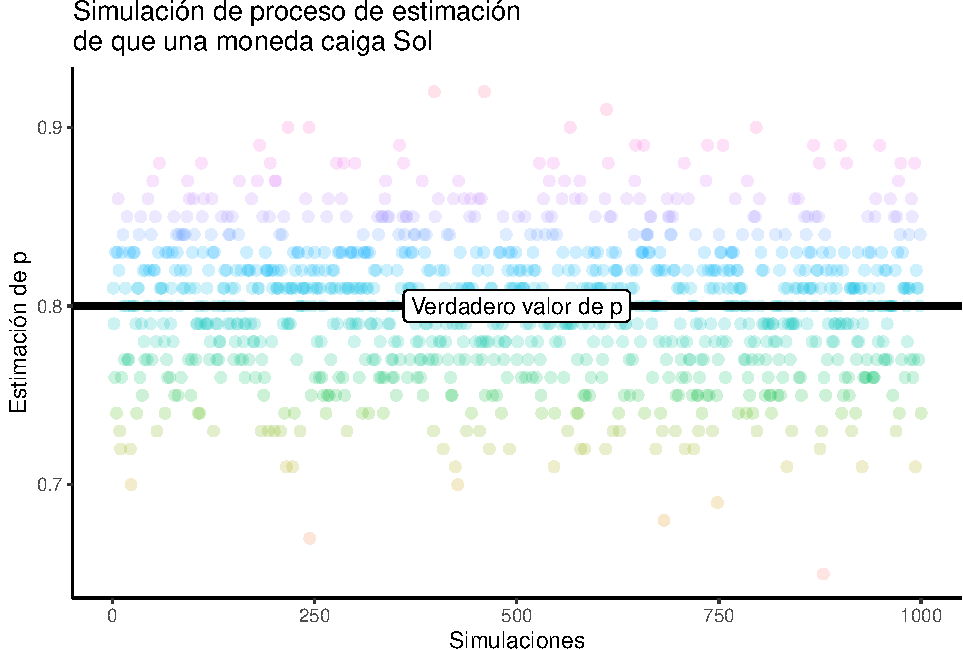
\includegraphics{Introduccion_a_Muestreo_files/figure-latex/unnamed-chunk-125-1.pdf}

\emph{¿Qué significa esto?} El que en promedio \(\hat{p}\) sea \(p\) (formalmente, que \(\mathbb{E}\big[\hat{p}\big] = p\)) significa que, si yo hago muchísimos experimentos (o procesos de muestreo) de la misma cosa, mi \(\hat{p}\) es un buen estimador porque en promedio le va a atinar. Empero, esto no dice nada de qué tan bueno es mi estimador \(\hat{p}\) para mi caso (mi muestra o mi experimento) específico. Puedes pensarlo con los exámenes: que alguien tenga un promedio de \emph{8} dice que en general le ha ido bien en los exámenes, pero no dice nada respecto al primer examen de cálculo que hizo (donde pudo tener \(10\) ó \(5\) para llegar a ese promedio de \(8\) \emph{pero no podemos saber de manera específica cuánto fue} ). Esto es igual: en promedio el estimador \(\hat{p}\) será \(p\) pero para un análisis específico \emph{no sabemos}.

\begin{quote}
\textbf{OJO} Los datos observados no son variables aleatorias: esos ya son fijos, ya los viste. Los \emph{posibles} datos observados sí son variables aleatorias ya que ellos, consisten en las variables que se \emph{pudieron} haber observado y te permiten calcular las probabilidades de tus datos observados bajo algún modelo. En el caso de la moneda, los datos observados son \(\vec{x} = \big( \text{Sol}, \text{Sol},\text{Sol},\text{Sol},\text{Sol},\text{Sol},\text{Sol},\text{Sol},\text{Sol},\text{Sol},\text{Águila}\big)^T\) pero los que se \emph{pudieron} haber observado son todas las \(\binom{n}{2}\) formas en las que la moneda pudo haber salido.
\end{quote}

\textbf{1. Estimación de una función de masa de probabilidad}
Formalmente, para una variable aleatoria discreta \(X\) que puede tomar los valores \(\{ a_1, a_2, \dots, a_{\ell} \}\) de la cual se observaron \(n\) realizaciones descritas mediante \(\vec{x} = (x_1, x_2, \dots, x_n)^T\) (observados, fijos, constantes). Definimos la \textbf{función de masa de probabilidad empírica} como:
\[
\hat{p}(x) = \begin{cases}
\\
\frac{1}{n} \sum_{i=1}^{n} \mathbb{I}_{\{a_1\}}(x_i) & \text{ si } x = a_1 \\ \\
\frac{1}{n} \sum_{i=1}^{n} \mathbb{I}_{\{a_2\}}(x_i) & \text{ si } x = a_2 \\ \\
\vdots \\ \\
\frac{1}{n} \sum_{i=1}^{n} \mathbb{I}_{\{a_{\ell}\}}(x_i) & \text{ si } x = a_{\ell} \\
0 & \text{ en otro caso}
\end{cases}
\]

donde se supone que \(\mathbb{P}(X = x) \approx \hat{p}(x)\). Notamos que lo anterior puede resumirse en:
\[
\hat{p}(x) = \frac{1}{n} \sum_{i=1}^{n} \mathbb{I}_{\{ x\}}(x_i)
\]

Análogamente, nota que para un conjunto (medible) \(A\), la aproximación para \(\mathbb{P}(X \in A)\) está dada por:

\[
\hat{p}(A) = \dfrac{1}{n}\sum\limits_{i=1}^{n} \mathbb{I}_A (x_i).
\]

Podemos graficar para la base de datos \texttt{conteo\_delitos} la probabilidad de que, dado que se cometió un delito, éste haya ocurrido en el dia \(d_i\) de diciembre. Para ello usamos un \texttt{geom\_col}:

\begin{Shaded}
\begin{Highlighting}[]
\FunctionTok{ggplot}\NormalTok{(conteo\_delitos) }\SpecialCharTok{+}
  \FunctionTok{geom\_col}\NormalTok{(}\FunctionTok{aes}\NormalTok{(}\AttributeTok{x =}\NormalTok{ fecha, }\AttributeTok{y =}\NormalTok{ n}\SpecialCharTok{/}\FunctionTok{sum}\NormalTok{(n), }\AttributeTok{fill =}\NormalTok{ n)) }\SpecialCharTok{+}
  \FunctionTok{scale\_fill\_gradient}\NormalTok{(}\StringTok{"Delito"}\NormalTok{, }\AttributeTok{low =} \StringTok{"orange"}\NormalTok{, }\AttributeTok{high =} \StringTok{"red"}\NormalTok{) }\SpecialCharTok{+}
  \FunctionTok{theme\_bw}\NormalTok{() }\SpecialCharTok{+}
  \FunctionTok{theme}\NormalTok{(}\AttributeTok{legend.position =} \StringTok{"none"}\NormalTok{) }\SpecialCharTok{+}
  \FunctionTok{labs}\NormalTok{(}
    \AttributeTok{y =} \StringTok{"p(x)"}\NormalTok{,}
    \AttributeTok{x =} \StringTok{"x"}\NormalTok{,}
    \AttributeTok{title =} \StringTok{"Aproximación a p(x)"}
\NormalTok{  )}
\end{Highlighting}
\end{Shaded}

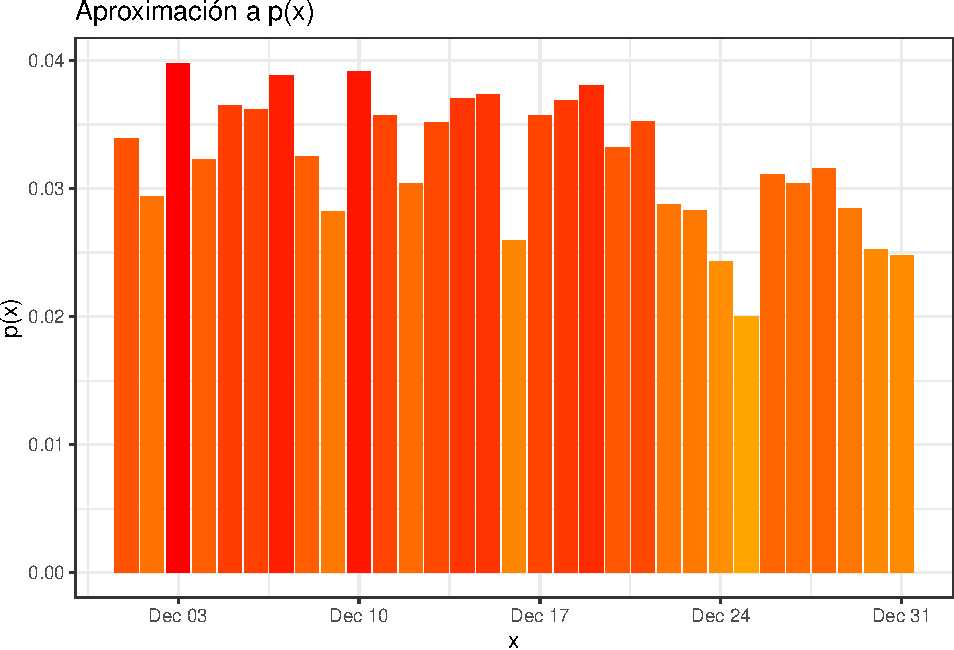
\includegraphics{Introduccion_a_Muestreo_files/figure-latex/unnamed-chunk-126-1.pdf}

Una propiedad interesante de la función de masa de probabilidad es que, en promedio, le atina al verdadero valor (lo que comentábamos antes de que \(\hat{p} = p\)). Es decir, suponiendo que \(X\) tiene una función de masa dada por:

\[
p(x) = \begin{cases}
p_1 & \text{ si } x = a_1 \\
p_2 & \text{ si } x = a_2 \\
\vdots \\
p_{\ell} & \text{ si } x = a_{\ell} \\
\end{cases}
\]

y suponiendo un vector de muestras posibles \(\vec{X} = (X_1, X_2, \dots, X_n)^T\) notamos que
\[
\mathbb{I}_{\{ a_j \}}(X_i) \sim \text{Bernoulli} (p_j)
\]

Luego para cualquier \(x\) se tiene que:

\[
\mathbb{E}\big[ \hat{p}(x)\big] = \mathbb{E}\bigg[ \dfrac{1}{n}\sum\limits_{i=1}^{n} \mathbb{I}_{\{ x \}}(X_i)  \bigg] = 
 \dfrac{1}{n}\sum\limits_{i=1}^{n}\mathbb{E}\big[ \mathbb{I}_{\{ x \}}(X_i)  \big] = \frac{1}{n} n \cdot p_j = p_j.
\]

\textbf{2. Función de distribución empírica}

Recuerda que para cualquier variable aleatoria \(X:\mathbb{R}\to\mathbb{R}\) existe su función de distribución \(F_X\) dada por:
\[
F_X(x) = \mathbb{P}(X \leq x)
\]
La idea de la función de distribución empírica es reconstruir (a partir de los datos observados) a \(F_X\). Para ello, notamos que queremos estimar
\[
\mathbb{P}(X \leq x) \qquad \forall x\in\mathbb{R}
\]
esto es equivalente a estimar:
\[
\mathbb{P}\big(X \in (-\infty, x] \big)
\]
y podemos aplicar la aproximación que usamos arriba para un conjunto \(A\):
\[
\mathbb{P}\big(X \in (-\infty, x] \big) \approx \sum\limits_{i=1}^n \mathbb{I}_{(-\infty, x]}(x_i)
\]

La función de distribución empírica está definida para un vector numérico \(\vec{x} = (x_1, x_2, \dots, x_n)^T\) por:
\[
\hat{F} (x) = \frac{1}{n} \sum\limits_{i=1}^{n} \mathbb{I}_{(-\infty, x]}(x_i)
\]

La función de distribución empírica es una función de distribución pues cumple las siguientes propiedades (demuéstralo):

\begin{enumerate}
\def\labelenumi{\arabic{enumi}.}
\item
  \(\lim_{x \to -\infty} \hat{F}(x) = 0\)
\item
  \(\lim_{x \to \infty} \hat{F}(x) = 1\)
\item
  Si \(x < y\) entonces \(\hat{F}(x) \leq \hat{F}(y)\) (no decreciente)
\item
  \(\hat{F}\) es continua por la derecha con límites por la izquierda (càdlàg).
\end{enumerate}

Para demostrar 4. basta con demostrar que para \(x_i\) fija, la función \(i(x) = \mathbb{I}_{(-\infty, x]}(x_i)\) es continua por la derecha con límites por la izquierda pues \(\hat{F}(x)\) es una suma de dichas funciones.

En particular, podemos notar que la función de distribución empírica \(\hat{F} (x)\) le atina a la función de distribución; es decir:

\[
\mathbb{E}\big[\hat{F} (x) \big] = F(x) 
\]

Para ello consideramos un vector de valores posibles \(\vec{X} = (X_1, X_2, \dots, X_n)^T\) donde las \(X_i\) tienen la misma distribución que \(X\). Y notamos que:
\[
\mathbb{I}_{(-\infty, x]}(X_i) \sim \textrm{Bernoulli}\big(F(x)\big)
\]
pues \(\mathbb{I}_{(-\infty, x]}(X_i) = 1\) si \(X_i \leq x\) y \(\mathbb{I}_{(-\infty, x]}(X_i) = 0\) si \(X_i > x\). Luego:
\[
\mathbb{P}\Big( \mathbb{I}_{(-\infty, x]}(X_i) = 1 \Big) = \mathbb{P}(X_i \leq x) = \mathbb{P}(X\leq x) = F(x)
\]

donde la igualdad del medio se sigue de que \(X_i\) y \(X\) tienen la misma distribución. Entonces:
\[
\mathbb{E}\big[ \hat{F}(x) \big] = \mathbb{E}\Big[ \dfrac{1}{n} \sum\limits_{i=1}^{n} \mathbb{I}_{(-\infty, x]}(X_i) \Big] = \dfrac{1}{n}\sum\limits_{i=1}^{n} \mathbb{E}\big[  \mathbb{I}_{(-\infty, x]}(X_i)\big] = \dfrac{1}{n} n \cdot F(x) = F(x)
\]

En \texttt{R} podemos calcular la función de distribución empírica con el comando \texttt{ecdf} el cual cuenta la cantidad de observaciones y regresa una función. Así, para la base de datos \texttt{conteo\_delitos} podemos calcular la función de distribución empírica \texttt{ecdf} asociada a la cantidad de delitos que se cometen en un día mediante:

\begin{Shaded}
\begin{Highlighting}[]
\NormalTok{Fgorro }\OtherTok{\textless{}{-}} \FunctionTok{ecdf}\NormalTok{(conteo\_delitos}\SpecialCharTok{$}\NormalTok{n)}
\end{Highlighting}
\end{Shaded}

De esta forma podemos calcular la probabilidad de que en un día se cometan menos de 500 delitos:

\begin{Shaded}
\begin{Highlighting}[]
\FunctionTok{Fgorro}\NormalTok{(}\DecValTok{500}\NormalTok{)}
\end{Highlighting}
\end{Shaded}

\begin{verbatim}
## [1] 0.09677419
\end{verbatim}

O bien podemos graficar la función:

\begin{Shaded}
\begin{Highlighting}[]
\NormalTok{x }\OtherTok{\textless{}{-}} \FunctionTok{seq}\NormalTok{(}\DecValTok{300}\NormalTok{, }\DecValTok{1000}\NormalTok{, }\AttributeTok{length.out =} \DecValTok{100}\NormalTok{)}
\NormalTok{y }\OtherTok{\textless{}{-}} \FunctionTok{Fgorro}\NormalTok{(x)}
\FunctionTok{ggplot}\NormalTok{() }\SpecialCharTok{+}
  \FunctionTok{geom\_step}\NormalTok{(}\FunctionTok{aes}\NormalTok{(}\AttributeTok{x =}\NormalTok{ x, }\AttributeTok{y =}\NormalTok{ y), }\AttributeTok{color =} \StringTok{"red"}\NormalTok{) }\SpecialCharTok{+}
  \FunctionTok{labs}\NormalTok{(}
    \AttributeTok{x =} \StringTok{"Número de carpetas de investigación (x)"}\NormalTok{,}
    \AttributeTok{y =} \StringTok{"Probabilidad de que en un día}\SpecialCharTok{\textbackslash{}n}\StringTok{se abran menos de x carpetas"}\NormalTok{,}
    \AttributeTok{title =} \StringTok{"Distribución acumulada de carpetas de investigación en CDMX"}
\NormalTok{  ) }\SpecialCharTok{+}
  \FunctionTok{theme\_minimal}\NormalTok{()}
\end{Highlighting}
\end{Shaded}

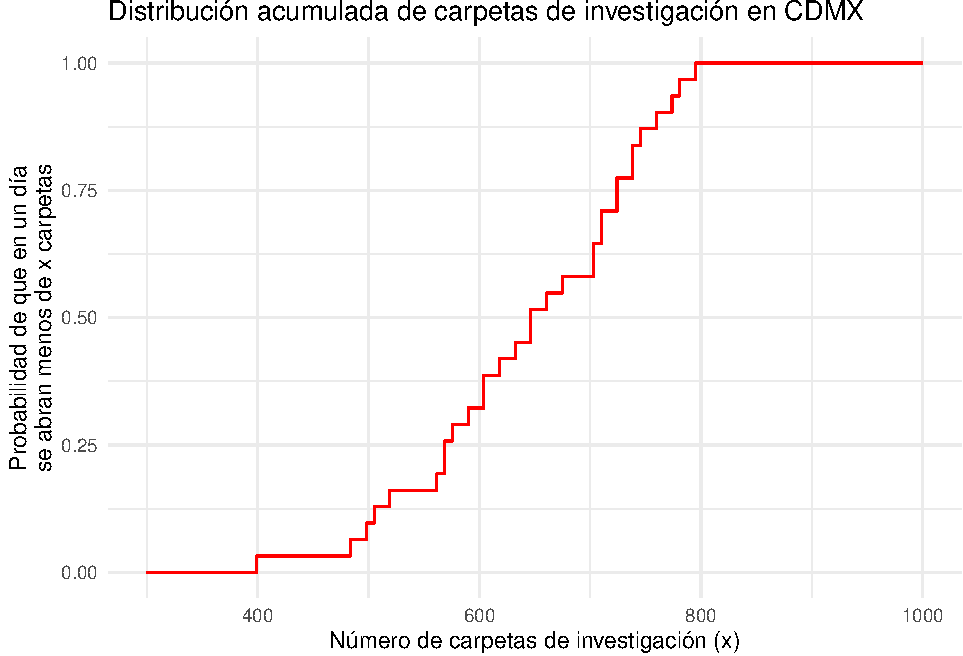
\includegraphics{Introduccion_a_Muestreo_files/figure-latex/unnamed-chunk-129-1.pdf}

Mediante simulaciones, podemos observar que \(\hat{F}\) realmente le atina a \(F\) como sigue:

\begin{Shaded}
\begin{Highlighting}[]
\CommentTok{\#Cantidad de simulaciones}
\NormalTok{nsim       }\OtherTok{\textless{}{-}} \DecValTok{100}

\CommentTok{\#Tamaño de la muestra en cada simulacion}
\NormalTok{n\_muestra  }\OtherTok{\textless{}{-}} \DecValTok{100}

\CommentTok{\#Valores a evaluar la función}
\NormalTok{x          }\OtherTok{\textless{}{-}} \FunctionTok{seq}\NormalTok{(}\SpecialCharTok{{-}}\DecValTok{5}\NormalTok{, }\DecValTok{5}\NormalTok{, }\AttributeTok{length.out =} \DecValTok{200}\NormalTok{)}

\CommentTok{\#Base de datos para guardar resultados de simulaciones}
\NormalTok{F\_simulado }\OtherTok{\textless{}{-}} \FunctionTok{data.frame}\NormalTok{(}\FunctionTok{matrix}\NormalTok{(}\ConstantTok{NA}\NormalTok{, }\AttributeTok{ncol =}\NormalTok{ nsim, }\AttributeTok{nrow =} \FunctionTok{length}\NormalTok{(x)))}

\ControlFlowTok{for}\NormalTok{ (i }\ControlFlowTok{in} \DecValTok{1}\SpecialCharTok{:}\NormalTok{nsim)\{}
\NormalTok{  valores\_simulados }\OtherTok{\textless{}{-}} \FunctionTok{rnorm}\NormalTok{(n\_muestra)}
\NormalTok{  F\_empirica        }\OtherTok{\textless{}{-}} \FunctionTok{ecdf}\NormalTok{(valores\_simulados)}
\NormalTok{  F\_simulado[,i]    }\OtherTok{\textless{}{-}} \FunctionTok{F\_empirica}\NormalTok{(x)}
\NormalTok{\}}

\NormalTok{F\_simulado}\SpecialCharTok{$}\NormalTok{Valor\_x }\OtherTok{\textless{}{-}}\NormalTok{ x}

\CommentTok{\#Cambiamos el formato de la base para graficar}
\NormalTok{F\_simulado }\OtherTok{\textless{}{-}}\NormalTok{ F\_simulado }\SpecialCharTok{\%\textgreater{}\%} \FunctionTok{pivot\_longer}\NormalTok{(}\AttributeTok{cols =} \SpecialCharTok{{-}}\NormalTok{Valor\_x)}

\FunctionTok{ggplot}\NormalTok{(F\_simulado) }\SpecialCharTok{+}
  \FunctionTok{geom\_step}\NormalTok{(}\FunctionTok{aes}\NormalTok{(}\AttributeTok{x =}\NormalTok{ Valor\_x, }\AttributeTok{y =}\NormalTok{ value, }\AttributeTok{color =}\NormalTok{ name), }\AttributeTok{alpha =} \FloatTok{0.1}\NormalTok{) }\SpecialCharTok{+}
  \FunctionTok{geom\_line}\NormalTok{(}\FunctionTok{aes}\NormalTok{(}\AttributeTok{x =}\NormalTok{ Valor\_x, }\AttributeTok{y =} \FunctionTok{pnorm}\NormalTok{(Valor\_x)), }\AttributeTok{color =} \StringTok{"black"}\NormalTok{) }\SpecialCharTok{+}
  \FunctionTok{theme\_classic}\NormalTok{() }\SpecialCharTok{+}
  \FunctionTok{theme}\NormalTok{(}\AttributeTok{legend.position =} \StringTok{"none"}\NormalTok{) }\SpecialCharTok{+}
  \FunctionTok{labs}\NormalTok{(}
    \AttributeTok{x =} \StringTok{"x"}\NormalTok{,}
    \AttributeTok{y =} \StringTok{"F(x)"}\NormalTok{,}
    \AttributeTok{title =} \StringTok{"Simulaciones de funciones de distribuciones acumuladas empíricas"}\NormalTok{,}
    \AttributeTok{subtitle =} \StringTok{"Para X \textasciitilde{} Normal(0,1)"}
\NormalTok{  )}
\end{Highlighting}
\end{Shaded}

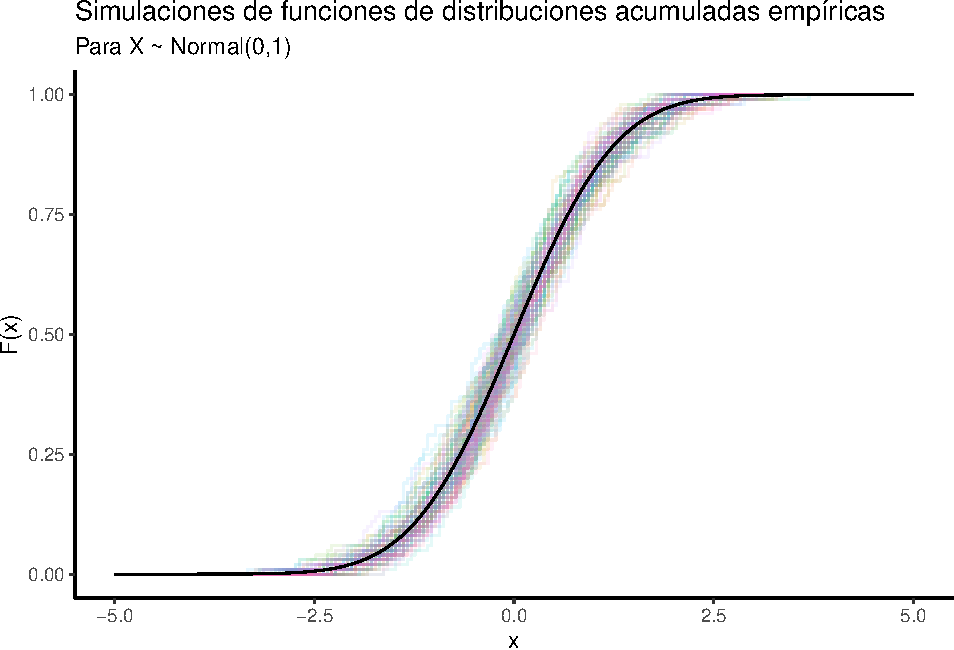
\includegraphics{Introduccion_a_Muestreo_files/figure-latex/unnamed-chunk-130-1.pdf}

\textbf{2. Histograma}
Para una variable aleatoria continua, la aproximación \(\hat{p}\) que hicimos no funciona (la masa siempre es \(0\)). Por lo que es necesario analizar alternativas para estudiar la densidad si suponemos que los datos pueden modelarse mediante algo continuo. Para construir un histograma consideremos \(\vec{x} = (x_1, x_2, \dots, x_n)^T\) y una constante \(h > 0\) llamada el \textbf{ancho de banda (binwidth)}. Sea \(\{ I_j \}\) una colección de intervalos no vacíos de \(\mathbb{R}\) tal que \(\cup_{j=1} I_j = \mathbb{R}\) e \(I_j \cap I_k = \emptyset\) (\emph{i.e.} los \(\{ I_j \}\) forman una partición de \(\mathbb{R}\)). Supongamos, además, los \(I_j\) son de la forma:
\[
I_j = \Big[\kappa + (j-1) h, \kappa + jh  \Big)
\]
para algún \(\kappa \in \mathbb{R}\) fijo. Sea
\[
n_j(\vec{x}) = \sum\limits_{i=1}^n \mathbb{I}_{I_j}(x_i)
\]
la cantidad de \(x_i\) en el intervalo \(I_j\).

Un histograma es la gráfica de la función (ver \protect\hyperlink{ref-panaretos2016statistics}{Panaretos} (\protect\hyperlink{ref-panaretos2016statistics}{2016})):
\[
\text{hist}_{\vec{x}}(x) = \frac{1}{n \cdot h} \sum\limits_{j} n_j(\vec{x}) \cdot \mathbb{I}_{I_j}(x)
\]

Una propiedad interesante de un histograma es que éste aproxima correctamente las probabilidades \(\mathbb{P}(X \in I_j)\). Para ver esto, consideramos un vector de valores posibles \(\vec{X} = (X_1, X_2, \dots, X_n)^T\) y que \(x\in I_j\), luego:

\[
\mathbb{E}\Big[ \int_{I_j} \text{hist}_{\vec{X}}(x) dx \Big] = \mathbb{E}\bigg[ \frac{1}{n \cdot h} \sum\limits_{j} n_j(\vec{X}) \cdot \int_{I_j} \mathbb{I}_{I_j}(x) dx \bigg] =  \frac{1}{n \cdot h} \sum\limits_{j} \mathbb{E}\big[ n_j(\vec{X}) \big] \cdot h  = \dfrac{1}{n}\sum\limits_{j} \mathbb{E}\big[ n_j(\vec{X}) \big]
\]
donde las \(n_j(\vec{X})\) son variables aleatorias en este caso y:
\[
\mathbb{E}\big[ n_j(\vec{X})\big] = \sum\limits_{i=1}^n \mathbb{E}\big[\mathbb{I}_{I_j}(X_i)\big] = \sum\limits_{i=1}^n\mathbb{P}(X_i \in I_j) = n \mathbb{P}(X \in I_j)
\]
donde la última igualdad se da pues las \(X_i\) tienen la misma distribución que \(X\). Luego:
\[
\mathbb{E}\Big[ \int_{I_j} \text{hist}_{\vec{X}}(x) dx \Big] = \mathbb{P}(X \in I_j)
\]
Es decir, el valor esperado del área bajo un histograma en un intervalo \(I_j\) coincide con la probabilidad de que \(X\) pertenezca a dicho intervalo.

Gráficamente:

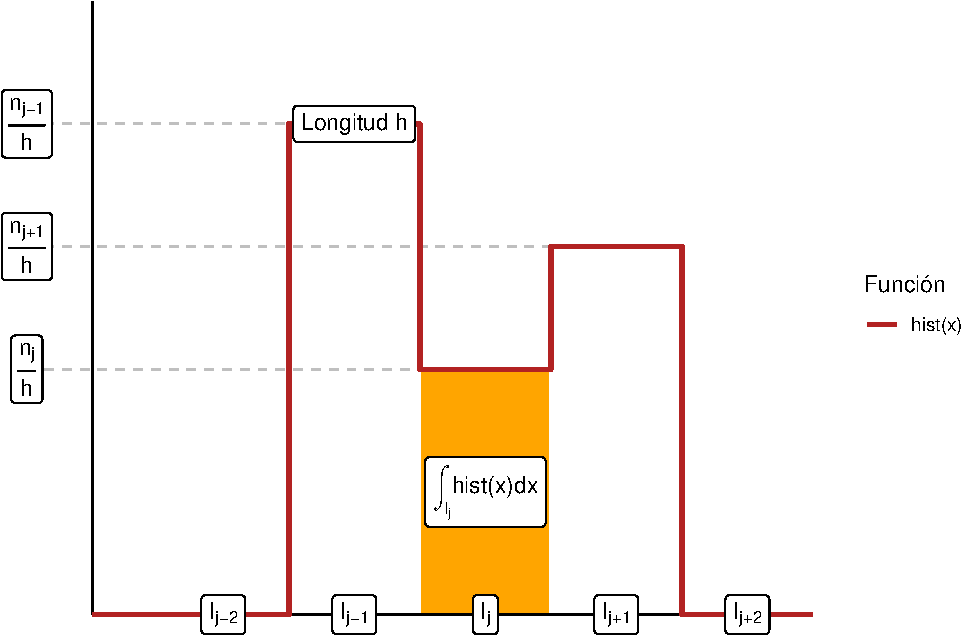
\includegraphics{Introduccion_a_Muestreo_files/figure-latex/unnamed-chunk-131-1.pdf}
En \texttt{R} podemos hacer un histograma a través de \texttt{geom\_histogram}. En este caso lo haremos de la latitud:

\begin{Shaded}
\begin{Highlighting}[]
\CommentTok{\#En este caso binwidth = h y kappa = boundary}
\FunctionTok{ggplot}\NormalTok{(datos) }\SpecialCharTok{+}
  \FunctionTok{geom\_histogram}\NormalTok{(}\FunctionTok{aes}\NormalTok{(}\AttributeTok{x =}\NormalTok{ latitud, }\AttributeTok{y =}\NormalTok{ ..density..), }
                 \AttributeTok{binwidth =} \FloatTok{0.02}\NormalTok{, }\AttributeTok{boundary =} \SpecialCharTok{{-}}\DecValTok{99}\NormalTok{,}
                 \AttributeTok{color =} \StringTok{"white"}\NormalTok{, }\AttributeTok{fill =} \StringTok{"purple"}\NormalTok{) }\SpecialCharTok{+}
  \FunctionTok{theme\_light}\NormalTok{() }
\end{Highlighting}
\end{Shaded}

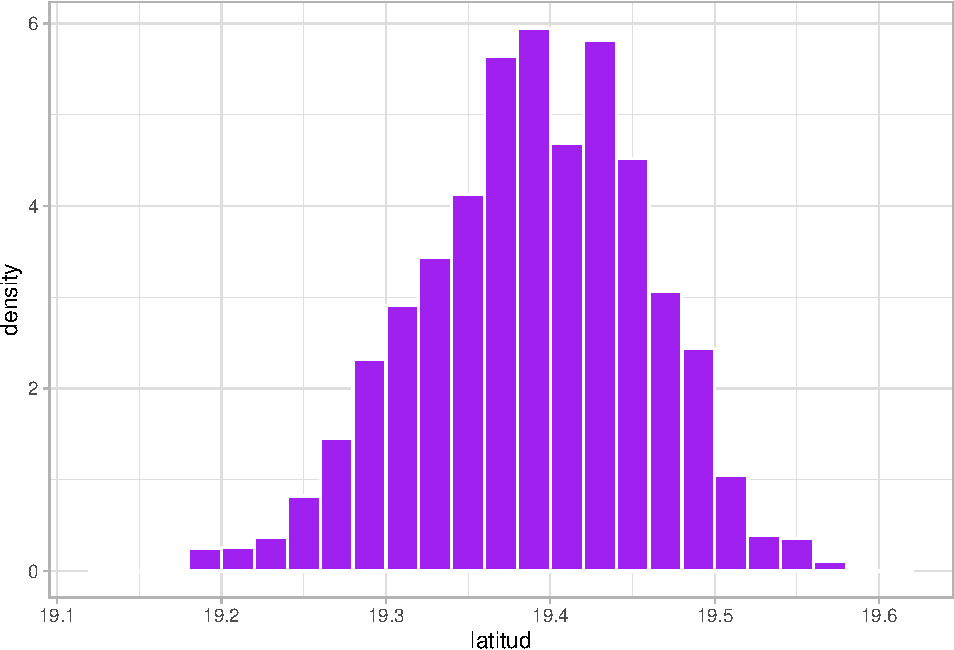
\includegraphics{Introduccion_a_Muestreo_files/figure-latex/unnamed-chunk-132-1.pdf}

\hypertarget{ejercicio-4}{%
\subsection{Ejercicio}\label{ejercicio-4}}

Considera la siguiente base de datos (obtenida de \href{https://stats.stackexchange.com/questions/51718/assessing-approximate-distribution-of-data-based-on-a-histogram}{Cross Validated}):

\begin{Shaded}
\begin{Highlighting}[]
\NormalTok{mis.datos }\OtherTok{\textless{}{-}} \FunctionTok{data.frame}\NormalTok{(}
  \AttributeTok{A =}  \FunctionTok{c}\NormalTok{(}\FloatTok{3.15}\NormalTok{, }\FloatTok{5.46}\NormalTok{, }\FloatTok{3.28}\NormalTok{, }\FloatTok{4.20}\NormalTok{, }\FloatTok{1.98}\NormalTok{, }\FloatTok{2.28}\NormalTok{, }\FloatTok{3.12}\NormalTok{, }\FloatTok{4.10}\NormalTok{, }\FloatTok{3.42}\NormalTok{, }\FloatTok{3.91}\NormalTok{, }
         \FloatTok{2.06}\NormalTok{, }\FloatTok{5.53}\NormalTok{, }\FloatTok{5.19}\NormalTok{, }\FloatTok{2.39}\NormalTok{, }\FloatTok{1.88}\NormalTok{, }\FloatTok{3.43}\NormalTok{, }\FloatTok{5.51}\NormalTok{, }\FloatTok{2.54}\NormalTok{, }\FloatTok{3.64}\NormalTok{, }\FloatTok{4.33}\NormalTok{, }
         \FloatTok{4.85}\NormalTok{, }\FloatTok{5.56}\NormalTok{, }\FloatTok{1.89}\NormalTok{, }\FloatTok{4.84}\NormalTok{, }\FloatTok{5.74}\NormalTok{, }\FloatTok{3.22}\NormalTok{, }\FloatTok{5.52}\NormalTok{, }\FloatTok{1.84}\NormalTok{, }\FloatTok{4.31}\NormalTok{, }\FloatTok{2.01}\NormalTok{, }
         \FloatTok{4.01}\NormalTok{, }\FloatTok{5.31}\NormalTok{, }\FloatTok{2.56}\NormalTok{, }\FloatTok{5.11}\NormalTok{, }\FloatTok{2.58}\NormalTok{, }\FloatTok{4.43}\NormalTok{, }\FloatTok{4.96}\NormalTok{, }\FloatTok{1.90}\NormalTok{, }\FloatTok{5.60}\NormalTok{, }\FloatTok{1.92}\NormalTok{),}
  \AttributeTok{B =}  \FunctionTok{c}\NormalTok{(}\FloatTok{2.90}\NormalTok{, }\FloatTok{5.21}\NormalTok{, }\FloatTok{3.03}\NormalTok{, }\FloatTok{3.95}\NormalTok{, }\FloatTok{1.73}\NormalTok{, }\FloatTok{2.03}\NormalTok{, }\FloatTok{2.87}\NormalTok{, }\FloatTok{3.85}\NormalTok{, }\FloatTok{3.17}\NormalTok{, }\FloatTok{3.66}\NormalTok{,}
         \FloatTok{1.81}\NormalTok{, }\FloatTok{5.28}\NormalTok{, }\FloatTok{4.94}\NormalTok{, }\FloatTok{2.14}\NormalTok{, }\FloatTok{1.63}\NormalTok{, }\FloatTok{3.18}\NormalTok{, }\FloatTok{5.26}\NormalTok{, }\FloatTok{2.29}\NormalTok{, }\FloatTok{3.39}\NormalTok{, }\FloatTok{4.08}\NormalTok{,}
         \FloatTok{4.60}\NormalTok{, }\FloatTok{5.31}\NormalTok{, }\FloatTok{1.64}\NormalTok{, }\FloatTok{4.59}\NormalTok{, }\FloatTok{5.49}\NormalTok{, }\FloatTok{2.97}\NormalTok{, }\FloatTok{5.27}\NormalTok{, }\FloatTok{1.59}\NormalTok{, }\FloatTok{4.06}\NormalTok{, }\FloatTok{1.76}\NormalTok{, }
         \FloatTok{3.76}\NormalTok{, }\FloatTok{5.06}\NormalTok{, }\FloatTok{2.31}\NormalTok{, }\FloatTok{4.86}\NormalTok{, }\FloatTok{2.33}\NormalTok{, }\FloatTok{4.18}\NormalTok{, }\FloatTok{4.71}\NormalTok{, }\FloatTok{1.65}\NormalTok{, }\FloatTok{5.35}\NormalTok{, }\FloatTok{1.67}\NormalTok{),}
  \AttributeTok{C =}  \FunctionTok{c}\NormalTok{(}\FloatTok{2.65}\NormalTok{, }\FloatTok{4.96}\NormalTok{, }\FloatTok{2.78}\NormalTok{, }\FloatTok{3.70}\NormalTok{, }\FloatTok{1.48}\NormalTok{, }\FloatTok{1.78}\NormalTok{, }\FloatTok{2.62}\NormalTok{, }\FloatTok{3.60}\NormalTok{, }\FloatTok{2.92}\NormalTok{, }\FloatTok{3.41}\NormalTok{,}
         \FloatTok{1.56}\NormalTok{, }\FloatTok{5.03}\NormalTok{, }\FloatTok{4.69}\NormalTok{, }\FloatTok{1.89}\NormalTok{, }\FloatTok{1.38}\NormalTok{, }\FloatTok{2.93}\NormalTok{, }\FloatTok{5.01}\NormalTok{, }\FloatTok{2.04}\NormalTok{, }\FloatTok{3.14}\NormalTok{, }\FloatTok{3.83}\NormalTok{,}
         \FloatTok{4.35}\NormalTok{, }\FloatTok{5.06}\NormalTok{, }\FloatTok{1.39}\NormalTok{, }\FloatTok{4.34}\NormalTok{, }\FloatTok{5.24}\NormalTok{, }\FloatTok{2.72}\NormalTok{, }\FloatTok{5.02}\NormalTok{, }\FloatTok{1.34}\NormalTok{, }\FloatTok{3.81}\NormalTok{, }\FloatTok{1.51}\NormalTok{, }
         \FloatTok{3.51}\NormalTok{, }\FloatTok{4.81}\NormalTok{, }\FloatTok{2.06}\NormalTok{, }\FloatTok{4.61}\NormalTok{, }\FloatTok{2.08}\NormalTok{, }\FloatTok{3.93}\NormalTok{, }\FloatTok{4.46}\NormalTok{, }\FloatTok{1.4}\NormalTok{, }\FloatTok{5.1}\NormalTok{, }\FloatTok{1.42}\NormalTok{),}
  \AttributeTok{D =}  \FunctionTok{c}\NormalTok{(}\FloatTok{2.40}\NormalTok{, }\FloatTok{4.71}\NormalTok{, }\FloatTok{2.53}\NormalTok{, }\FloatTok{3.45}\NormalTok{, }\FloatTok{1.23}\NormalTok{, }\FloatTok{1.53}\NormalTok{, }\FloatTok{2.37}\NormalTok{, }\FloatTok{3.35}\NormalTok{, }\FloatTok{2.67}\NormalTok{, }\FloatTok{3.16}\NormalTok{,}
         \FloatTok{1.31}\NormalTok{, }\FloatTok{4.78}\NormalTok{, }\FloatTok{4.44}\NormalTok{, }\FloatTok{1.64}\NormalTok{, }\FloatTok{1.13}\NormalTok{, }\FloatTok{2.68}\NormalTok{, }\FloatTok{4.76}\NormalTok{, }\FloatTok{1.79}\NormalTok{, }\FloatTok{2.89}\NormalTok{, }\FloatTok{3.58}\NormalTok{,}
         \FloatTok{4.10}\NormalTok{, }\FloatTok{4.81}\NormalTok{, }\FloatTok{1.14}\NormalTok{, }\FloatTok{4.09}\NormalTok{, }\FloatTok{4.99}\NormalTok{, }\FloatTok{2.47}\NormalTok{, }\FloatTok{4.77}\NormalTok{, }\FloatTok{1.09}\NormalTok{, }\FloatTok{3.56}\NormalTok{, }\FloatTok{1.26}\NormalTok{, }
         \FloatTok{3.26}\NormalTok{, }\FloatTok{4.56}\NormalTok{, }\FloatTok{1.81}\NormalTok{, }\FloatTok{4.36}\NormalTok{, }\FloatTok{1.83}\NormalTok{, }\FloatTok{3.68}\NormalTok{, }\FloatTok{4.21}\NormalTok{, }\FloatTok{1.15}\NormalTok{, }\FloatTok{4.85}\NormalTok{, }\FloatTok{1.17}\NormalTok{)}
\NormalTok{)}
\end{Highlighting}
\end{Shaded}

Grafica un histograma de las variables \texttt{A}, \texttt{B}, \texttt{C} y \texttt{D} de dicha base con un ancho de banda (binwidth) igual a \texttt{1}.

\begin{enumerate}
\def\labelenumi{\alph{enumi}.}
\item
  ¿Podemos concluir la forma de la distribución a partir del histograma? Es decir ¿hay distribuciones sesgadas a la izquierda, a la derecha, uniformes, centradas o con colas pesadas?
\item
  Realiza el mismo histograma pero ahora con un ancho de banda de 0.25 ¿por qué hubo cambios?
\item
  Analiza la base de datos (los valores en función de la columna A) y concluye.
\end{enumerate}

\textbf{3. Densidad kernel}
Un histograma tiene muchos bemoles: en particular, es necesario decidir quién es \(h\) y quién \(\kappa\) y no hay una regla clara de cómo hacerlo. La densidad \texttt{kernel} es un intento de mejorar esta situación. Para ello recordamos que si \(X\) es una variable aleatoria continua con densidad \(F\) entonces:
\[
f(x) = F'(x) = \lim_{h \to 0} \dfrac{F(x + h) - F(x - h)}{2h}
\]
Por lo que para un \(h\) positiva con \(h \approx 0\) tenemos que:
\[
f(x) \approx \dfrac{F(x + h) - F(x - h)}{2h} 
\]
En el caso de un vector de observaciones \(\vec{x} = (x_1, x_2, \dots, x_n)^T\) recordamos que podemos asociar una función de distribución empírica \(\hat{F}\) y por tanto obtener el \emph{estimador de Rosenblatt} de la densidad \(f\) mediante:
\[
\hat{f}(x) =  \dfrac{\hat{F}(x + h) -\hat{F}(x - h)}{2h} 
\]
Podemos reescribir esto como:
\[
\hat{f}(x) =  \dfrac{1}{2nh} \sum\limits_{i = 1}^n \mathbb{I}_{(x-h, x+h]}(x_i) = \dfrac{1}{nh}\sum\limits_{i = 1}^n K\Big( \frac{x_i - x}{h}\Big)
\]
donde:
\[
K(u) = \frac{1}{2} \mathbb{I}_{(-1, 1]}(u)
\]

se conoce como el \emph{kernel rectangular}. Una vez que llegamos hasta este punto notamos que para cualquier \(K\) que cumple:

\begin{enumerate}
\def\labelenumi{\arabic{enumi}.}
\item
  \(\int\limits_{-\infty}^{\infty} K(u) du = 1\)
\item
  \(K(u) \geq 0\)
\end{enumerate}

la función \(\hat{f}\) es una función de densidad. La función \(\hat{f}\) se conoce como el \emph{estimador de densidad del kernel K}. Algunos ejemplos de kernels \(K\) son:

\begin{enumerate}
\def\labelenumi{\arabic{enumi}.}
\item
  \textbf{Rectangular:} \(K(u) = \frac{1}{2} \mathbb{I}_{(-1, 1]}(u)\)
\item
  \textbf{Triangular:} \(K(u) = (1 - |u|) \mathbb{I}_{(-1, 1]}(u)\)
\item
  \textbf{Epanechnikov:} \(K(u) = \frac{3}{4}(1 - u^2) \mathbb{I}_{(-1, 1]}(u)\)
\item
  \textbf{Gaussiano:} \(K(u) = \frac{1}{\sqrt{2\pi}}\text{exp}(-u^2/2)\)
\end{enumerate}

\begin{quote}
\textbf{OJO} No confundir el Kernel \(K\) (que es una función que integra a \(1\)) con \emph{función de densidad kernel} que es una función de los datos que utiliza un kernel y es una densidad por sí misma.
\end{quote}

En \texttt{R} podemos calcular la densidad \texttt{kernel} en \texttt{n} puntos con relativa facilidad mediante \texttt{density}:

\begin{Shaded}
\begin{Highlighting}[]
\NormalTok{densidad\_kernel }\OtherTok{\textless{}{-}} \FunctionTok{density}\NormalTok{(datos}\SpecialCharTok{$}\NormalTok{latitud, }\AttributeTok{kernel =} \StringTok{"gaussian"}\NormalTok{, }\AttributeTok{n =} \DecValTok{700}\NormalTok{,}
                           \AttributeTok{na.rm =} \ConstantTok{TRUE}\NormalTok{)}
\end{Highlighting}
\end{Shaded}

Nota que \texttt{R} en automático preselecciona los valores de \texttt{h} mediante un criterio preprogramado de optimización. Podemos ver dicha densidad gráficamente (y compararla con un histograma):

\begin{Shaded}
\begin{Highlighting}[]
\FunctionTok{ggplot}\NormalTok{(datos) }\SpecialCharTok{+}
  \FunctionTok{geom\_histogram}\NormalTok{(}\FunctionTok{aes}\NormalTok{(}\AttributeTok{x =}\NormalTok{ latitud, }\AttributeTok{y =}\NormalTok{ ..density..), }
                 \AttributeTok{binwidth =} \FloatTok{0.01}\NormalTok{, }\AttributeTok{boundary =} \DecValTok{19}\NormalTok{,}
                 \AttributeTok{fill =} \StringTok{"purple"}\NormalTok{, }\AttributeTok{color =} \StringTok{"white"}\NormalTok{) }\SpecialCharTok{+}
  \FunctionTok{geom\_density}\NormalTok{(}\FunctionTok{aes}\NormalTok{(}\AttributeTok{x =}\NormalTok{ latitud), }\AttributeTok{kernel =} \StringTok{"gaussian"}\NormalTok{, }\AttributeTok{size =} \FloatTok{1.5}\NormalTok{) }\SpecialCharTok{+}
  \FunctionTok{theme\_bw}\NormalTok{()}
\end{Highlighting}
\end{Shaded}

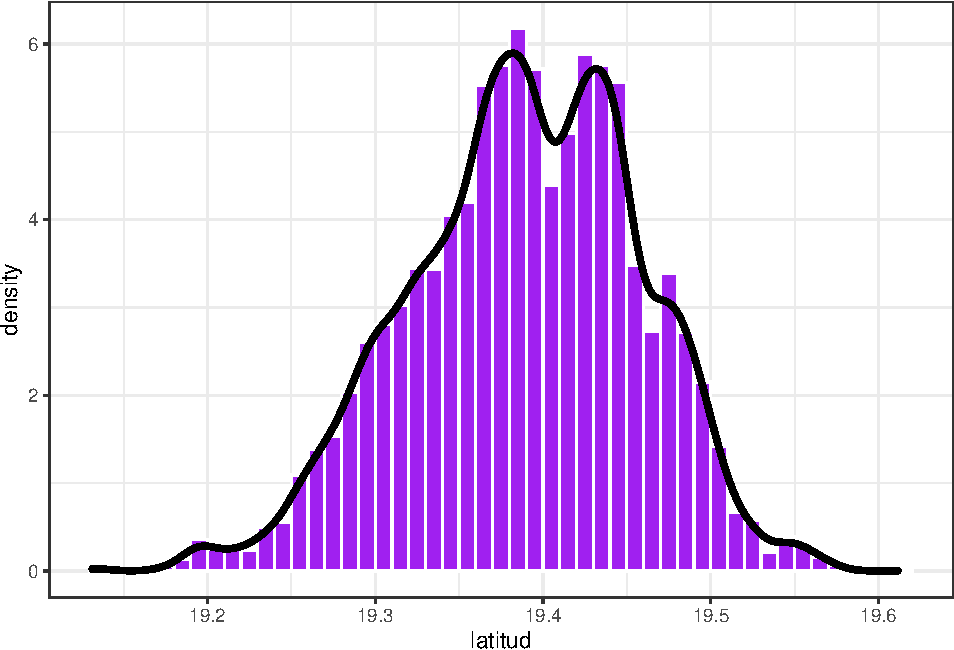
\includegraphics{Introduccion_a_Muestreo_files/figure-latex/unnamed-chunk-135-1.pdf}

Esto no se queda ahí, podemos generalizar el concepto de kernel a dos dimensiones para aproximar una función de densidad \(f(x,y)\) de dos variables aleatorias sí tenemos dos vectores \(\vec{x}\) y \(\vec{y}\) y calculamos:

\[
\hat{f}(x,y) =\dfrac{1}{nh^2} \sum\limits_{i = 1}^n K \Big( \frac{x_i - x}{h}\Big) K \Big( \frac{y_i - y}{h}\Big)
\]

En particular esto nos permite generar una densidad en \texttt{R} para saber en qué coordenadas de latitud y longitud ocurren más los delitos:

\begin{Shaded}
\begin{Highlighting}[]
\FunctionTok{ggplot}\NormalTok{(datos) }\SpecialCharTok{+}
  \FunctionTok{geom\_point}\NormalTok{(}\FunctionTok{aes}\NormalTok{(}\AttributeTok{x =}\NormalTok{ longitud, }\AttributeTok{y =}\NormalTok{ latitud), }\AttributeTok{alpha =} \FloatTok{0.025}\NormalTok{) }\SpecialCharTok{+}
  \FunctionTok{geom\_density\_2d\_filled}\NormalTok{(}\FunctionTok{aes}\NormalTok{(}\AttributeTok{x =}\NormalTok{ longitud, }\AttributeTok{y =}\NormalTok{ latitud), }\AttributeTok{alpha =} \FloatTok{0.75}\NormalTok{) }\SpecialCharTok{+}
  \FunctionTok{geom\_density2d}\NormalTok{(}\FunctionTok{aes}\NormalTok{(}\AttributeTok{x =}\NormalTok{ longitud, }\AttributeTok{y =}\NormalTok{ latitud)) }\SpecialCharTok{+}
  \FunctionTok{theme\_void}\NormalTok{()}
\end{Highlighting}
\end{Shaded}

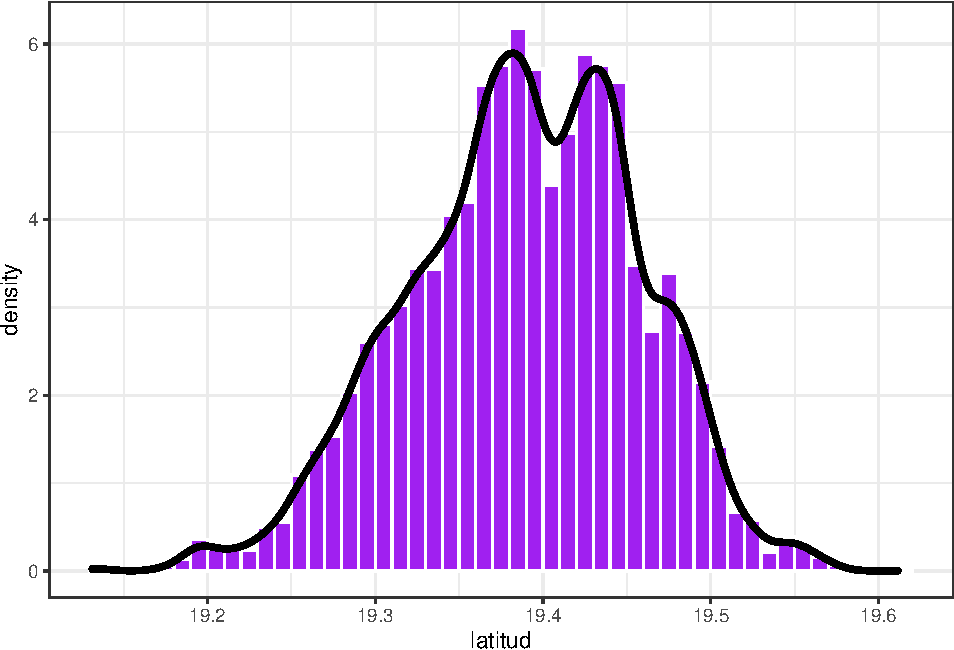
\includegraphics{Introduccion_a_Muestreo_files/figure-latex/unnamed-chunk-136-1.pdf}

\hypertarget{ejercicio-sugerido}{%
\subsection{Ejercicio sugerido}\label{ejercicio-sugerido}}

Este ejercicio es para que tengas la seguridad de que comprendiste los conceptos previos y sabes calcularlos. Es tedioso pero bueno para aclarar dudas.

Considera la siguiente base de datos:

\begin{table}
\centering
\begin{tabular}{r|r|l|l}
\hline
x & y & z & w\\
\hline
\cellcolor{gray!6}{1} & \cellcolor{gray!6}{-100} & \cellcolor{gray!6}{Rojo} & \cellcolor{gray!6}{Bueno}\\
\hline
2 & -2 & Azul & Malo\\
\hline
\cellcolor{gray!6}{3} & \cellcolor{gray!6}{2} & \cellcolor{gray!6}{Azul} & \cellcolor{gray!6}{Regular}\\
\hline
2 & 3 & Rojo & Bueno\\
\hline
\cellcolor{gray!6}{1} & \cellcolor{gray!6}{1} & \cellcolor{gray!6}{Verde} & \cellcolor{gray!6}{Bueno}\\
\hline
3 & 4 & Amarillo & Malo\\
\hline
\end{tabular}
\end{table}

Calcula \textbf{a mano} (es decir puedes usar calculadora pero no lo calcules en \texttt{R}) y luego \textbf{verifica tus cálculos haciéndolo en \texttt{R}}:

\begin{enumerate}
\def\labelenumi{\arabic{enumi}.}
\item
  El total de \(\vec{x}\)
\item
  La media y varianza de \(\vec{y}\)
\item
  La curtosis y la asimetría de \(\vec{x}\) (su media es 2 y su varianza 0.8). Determina si tiene un sesgo a la derecha, a la izquierda o ninguno.
\item
  Determina mediante la curtosis si \(\vec{x}\) tiene colas más pesadas que \(\vec{y}\).
\item
  Calcula el cuantil \(0.25\) y el \(0.75\) de \(\vec{y}\) así como su rango intercuartílico (IQR).
\item
  ¿Hay valores atípicos (\emph{outliers}) en \(\vec{y}\)? En caso afirmativo, determina cuáles son.
\item
  ¿Cuál es el rango de \(\vec{y}\)? (no confundir con el IQR).
\item
  Determina la moda de \(\vec{z}\)
\item
  Determina la mediana de \(\vec{x}\).
\item
  Determina la MAD de \(\vec{x}\)
\item
  Realiza el conteo de cuáles \(\vec{z}\) pertenecen al conjunto \(A = \{ \text{Rojo}, \text{Amarillo} \}\)
\item
  Realiza una tabla de contingencia de \(\vec{w}\) y \(\vec{z}\).
\item
  Determina la distribución frecuencial (observada) marginal de \(\vec{w}\).
\item
  Realiza una tabla de frecuencias de \(\vec{w}\) y \(\vec{z}\).
\item
  Calcula el riesgo relativo de estar en un choque dado que manejas en CDMX a partir de los datos en la tabla:
\end{enumerate}

\begin{table}
\centering
\begin{tabular}{l|r|r|r}
\hline
  & CDMX & MTY & Total\\
\hline
\cellcolor{gray!6}{Chocó} & \cellcolor{gray!6}{1100} & \cellcolor{gray!6}{4000} & \cellcolor{gray!6}{5100}\\
\hline
No Chocó & 120 & 5080 & 5200\\
\hline
\cellcolor{gray!6}{Total} & \cellcolor{gray!6}{1220} & \cellcolor{gray!6}{9080} & \cellcolor{gray!6}{10300}\\
\hline
\end{tabular}
\end{table}

Interpreta tu resultado.

\begin{enumerate}
\def\labelenumi{\arabic{enumi}.}
\setcounter{enumi}{15}
\item
  De la tabla anterior calcula la razón de momios asociada a chocar dado que manejas en CDMX. Interprétala.
\item
  Calcula la correlación de Bravais Pearson de \(\vec{x}\) y \(\vec{y}\). Interpreta.
\item
  Obtén la correlación de Spearman de \(\vec{x}\) y \(\vec{y}\)
\item
  Para \(\vec{w}\) y \(\vec{x}\) obtén la \(\tau\) de Kendall (son 15 comparaciones para generarla)
\item
  Descartando el \emph{outlier} de \(\vec{y}\) (y su \(\vec{x}\) asociada), ajusta un modelo lineal \(\hat{y} = \hat{\beta}_1 x + \hat{\beta}_0\) y grafícalo para ver qué tan buen modelo es.
\item
  Realiza una gráfica de caja (boxplot) para \(\vec{y}\)
\item
  Realiza un scatterplot para la submatriz \(Z_{(x,y)}\).
\item
  Realiza una gráfica de líneas para \(Z_{(x,y)}\) identificando la función de interpolación lineal \(f(x)\) asociada.
\item
  Realiza una gráfica de barras de \(\vec{w}\) especificando quiénes son los \(a_i\) y los \(n_j\).
\item
  Estima mediante \(\hat{p}\) la función de probabilidad de \(\vec{w}\).
\item
  Identifica la función de distribución empírica para \(\vec{x}\), \(\hat{F}\) y grafícala.
\item
  Realiza un histograma con \(h = 2\) para \(x\). Toma \(\kappa = 4\).
\item
  Ajusta una densidad kernel a \(\vec{x}\) con \(h = 1\) y usando un kernel \(K\) triangular. Calcula \(\hat{f}(x)\) para \(x = 0,1,2,3,4\).
\end{enumerate}

\hypertarget{ejercicios-del-capuxedtulo}{%
\section{Ejercicios del capítulo}\label{ejercicios-del-capuxedtulo}}

\begin{enumerate}
\def\labelenumi{\arabic{enumi}.}
\tightlist
\item
  Dado \(\vec{x}\) vector de variables ordinales, obtén una expresión matemática para los siguientes estadísticos:

  \begin{enumerate}
  \def\labelenumii{\alph{enumii}.}
  \tightlist
  \item
    La media de las diferencias entre las \(x_i\) quitando la de \(x_k\) consigo misma.
  \item
    El valor numérico o categoría menos común en \(\vec{x}\).
  \item
    Si ordenamos todos los valores, la diferencia más alta entre algún \(x_{(i)}\) y su sucesor: \(x_{(i+1)}\).
  \item
    Este cálculo de \texttt{R} para una S dada como vector numérico:
  \end{enumerate}
\end{enumerate}

\begin{Shaded}
\begin{Highlighting}[]
\CommentTok{\#x es la muestra; x \textless{}{-} c(x1,x2, ..., xn)}
\NormalTok{datos\_nuevos }\OtherTok{\textless{}{-}} \FunctionTok{c}\NormalTok{()}
\ControlFlowTok{for}\NormalTok{ (i }\ControlFlowTok{in} \DecValTok{1}\SpecialCharTok{:}\FunctionTok{length}\NormalTok{(x))\{}
\NormalTok{    datos\_nuevos }\OtherTok{\textless{}{-}} \FunctionTok{c}\NormalTok{(datos\_nuevos, x[i]}\SpecialCharTok{\^{}}\NormalTok{i)}
\NormalTok{\}}
\FunctionTok{mean}\NormalTok{(datos\_nuevos) }\CommentTok{\#Este valor es el que me interesa}
\end{Highlighting}
\end{Shaded}

\begin{enumerate}
\def\labelenumi{\arabic{enumi}.}
\setcounter{enumi}{1}
\item
  Demuestra que:
  \[
  \sigma^2_{\vec{x}} = \dfrac{1}{n}\sum\limits_{i=1}^n x_i^2 - \bar{x}^2
  \]
\item
  Para unos datos observados numéricos \(\vec{x} = (x_1, x_2, \dots, x_n)^T\) se tiene que las \(x\) toman el valor \(a_{x,1}\) \(n_{x,1}\) veces, el valor \(a_{x,2}\), \(n_{x,2}\) veces y el valor \(a_{x,\ell}\), \(n_{x,\ell}\) veces (\(n_j \geq 0\), \(0 < \ell \leq n\) y \(\sum_{j=1}^{\ell} n_j = n\)). Demuestra que:
  \[
   \bar{x} = \dfrac{1}{\sum_{j = 1}^{\ell} n_{j}} \cdot \sum\limits_{j=1}^{\ell} n_j a_j 
  \]
\item
  Sea \(n\) impar y \(f\) una función estrictamente decreciente.

  \begin{enumerate}
  \def\labelenumii{\alph{enumii}.}
  \tightlist
  \item
    Demuestra que si \(x_*\) es la mediana de \(\vec{x} = ( x_1, x_2,\dots, x_n)^T\) entonces \(f(x_*)\) es la mediana de \(\Tilde{\vec{x}} = \big( f(x_1), f(x_2),\dots, f(x_n)\big)^T\).
  \item
    Demuestra que si \(\bar{x}\) es la media observada de \(\vec{x} = ( x_1, x_2,\dots, x_n)^T\) y \(f(\bar{x})\) es la media observada de \(\Tilde{\vec{x}} = \big( f(x_1), f(x_2),\dots, f(x_n)\big)^T\) y además \(f\) es diferenciable, entonces \(f(x) = a \cdot x + b\) (es decir es una transformación afín). \textbf{Hint} Deriva.
  \end{enumerate}
\item
  Sea \(\phi\) una función convexa. Demuestra que:
  \[
   \phi \Big( \bar{x} \Big) \leq \dfrac{1}{n}\sum\limits_{i=1}^n \phi(x_i)
  \]
  \textbf{Hint} Deriva. Recuerda que si \(\phi\) es convexa, para \(0 \leq \alpha \leq 1\) se tiene que:
  \[
  \phi\big(\alpha x + (1-\alpha) y\big) \leq \alpha \phi(x) + (1-\alpha)\phi(y)
  \]
\item
  Sea \(\hat{p}_R(x)\) la densidad kernel asociada a \(\vec{x} = (x_1, x_2, \dots, x_n)\) con un núcleo (kernel) \(K(u) \geq 0\) y \(h > 0\). Demuestra:

  \begin{enumerate}
  \def\labelenumii{\alph{enumii}.}
  \tightlist
  \item
    \(\hat{p}_h(x)\) es una función de densidad de probabilidad (\textit{i.e.} integra a \(1\)).
  \item
    Determina la media de una variable aleatoria \(X\) que se distribuye con densidad \(\hat{p}_h(x)\) bajo: Kernel triangular.
  \item
    Determina la varianza de una variable aleatoria \(X\) que se distribuye con densidad \(\hat{p}_h(x)\) bajo: Kernel Epanechnikov
  \end{enumerate}
\item
  Sea \(\text{hist}_{\vec{x}}\) la función de histograma para un vector numérico \(\vec{x}\) con \(h > 0\), \(\kappa \in \mathbb{R}\) fijos y una partición \(\{I_j\}_{j \in \mathbb{Z}}\). Demuestra que \(\text{hist}_{\vec{x}}\) es una función de densidad.
\item
  Demuestra que para \(\vec{x} = (x_1, x_2, \dots, x_n)^T\) la función de distribución empírica \(\hat{F}(x)\) es una función de distribución acumulada; es decir:

  \begin{enumerate}
  \def\labelenumii{\alph{enumii}.}
  \tightlist
  \item
    \(\lim_{x \to -\infty} \hat{F} (x) = 0\)
  \item
    \(\lim_{x \to \infty} \hat{F} (x) = 1\)
  \item
    \(\lim_{x \to x_0^+} \hat{F} (x) = \hat{F} (x_0)\) (continua por la derecha)
  \item
    \(\lim_{x \to x_0^-} \hat{F} (x)\) existe
  \item
    \(F_n (x)\) es no decreciente.
  \end{enumerate}
\item
  La tabla \ref{tab:my_label} muestra datos observados del PIB de un país en billones de dólares:
\end{enumerate}

\begin{table}
\centering
\begin{tabular}{r|r}
\hline
Año & PIB\\
\hline
\cellcolor{gray!6}{2000} & \cellcolor{gray!6}{0.5}\\
\hline
2005 & 1.2\\
\hline
\cellcolor{gray!6}{2010} & \cellcolor{gray!6}{1.5}\\
\hline
2015 & 2.1\\
\hline
\end{tabular}
\end{table}

Ajusta una parábola \(q (x) = a \cdot x^2 + b\cdot x + c\) para obtener la mejor parábola que ajuste esos puntos. ¿Qué valor de PIB se espera para el 2020 bajo este modelo?

\begin{enumerate}
\def\labelenumi{\arabic{enumi}.}
\setcounter{enumi}{9}
\item
  Demuestra que si \(\vec{x} = -\vec{y}\) (dos vectores numéricos) la correlación de Spearman entre ambos es \(-1\).
\item
  Para una variable aleatoria \(T\) que representa un tiempo, se define una función de supervivencia como la probabilidad de que \(T\) dure más que un cierto tiempo \(t\); es decir:
  \begin{equation}\nonumber
  S(t) = \mathbb{P}(T > t)
  \end{equation}
  Construye \(\hat{S}\) una aproximación empírica a la función de supervivencia \(S\) tal que \(\mathbb{E}[\hat{S}(t)] = S(t)\). Demuestra este último resultado.
\item
  Demuestra que \(\text{Var}\big[ \hat{F}(x) \big] = \frac{1}{n} F(x) \big( 1 - F(x) \big)\).
\item
  Recuerda que para dos variables aleatorias \(X\) y \(Y\) se define la covarianza \(\text{Cov}(X,Y) = \mathbb{E}[XY] - \mathbb{E}[X]\mathbb{E}[Y]\). Calcula entonces la covarianza dada por \(\text{Cov}\big(\hat{p}(u), \hat{p}(v)\big)\).
\item
  Demuestra que si \(X\) es independiente de \(Y\) entonces \(\mathbb{I}_A(X)\) es independiente de \(\mathbb{I}_A(Y)\). Recuerda que dos variables aleatorias \(X\), \(Y\) son independientes si y sólo si \(\mathbb{P}(X \in A, Y \in B) = \mathbb{P}(X \in A) \mathbb{P}(Y \in B)\) para conjuntos \(A,B\) medibles.
\item
  Sean \(\rho\) la \(\rho\) de Spearman y \(\tau\) la \(\tau\) de Kendall para dos vectores ordinales \(\vec{x}\) y \(\vec{y}\). Demuestra que:
  \[
  \frac{1 + \rho}{2} \geq \Big( \frac{1 + \tau}{2} \Big)^2
  \]
\item
  Da un ejemplo de vector \(\vec{x}\) de al menos dos entradas tal que \(\text{MAD}_{\vec{x}} \geq \sigma_{\vec{x}}\)
\item
  Demuestra que \(\text{MAD}_{\vec{x}} = 0 \Leftrightarrow \sigma_{\vec{x}} = 0\) para el mismo vector \(\vec{x}\).
\item
  Si un vector \(\vec{x}\) tiene \(3\) entradas, media \(\bar{x} = 1\) y varianza \(\sigma_{\vec{x}} = 1\) y además se sabe que su curtosis es \(1\), ¿quién es \(\vec{x}\)?
\item
  Bajo la correlación de Pearson demuestra que para vectores \(\vec{x}, \vec{y}\) y \(\vec{z}\) si \(\rho_{\vec{x},\vec{y}} = 1\) y \(\rho_{\vec{x},\vec{z}} = 1\) entonces \(\rho_{\vec{y},\vec{z}} = 1\)
\item
  Sean \(\vec{w}, \vec{x}, \vec{y}, \vec{z} \in\mathbb{R}^n\) y \(a,b,c,d\in\mathbb{R}\) demuestra que:
  \[
  \rho(a \vec{x} + b \vec{w}, c \vec{y} + d \vec{z}) = K_1\cdot\rho(\vec{x}, \vec{y}) + K_2\cdot\rho(\vec{w}, \vec{y}) + K_3\cdot\rho(\vec{x}, \vec{z}) + K_4\cdot\rho(\vec{w}, \vec{z}) 
  \]
  para algunas constantes \(K_1, K_2, K_3, K_4\); donde, además, \(\rho\) es la correlación de Pearson.
\item
  Sean \(\vec{x} = (x_1,x_2, \dots, x_n)^T\) el vector de los datos observados (fijo) y \(\vec{X} = (X_1,X_2, \dots, X_n)^T\) el vector de los datos posibles (aleatorio). Supongamos que las entradas de \(\vec{X}\) son independientes e idénticamente distribuidas con la misma distribución de \(X\) con media \(\mu\) y varianza \(\sigma^2\).

  \begin{enumerate}
  \def\labelenumii{\alph{enumii}.}
  \tightlist
  \item
    Demuestra que \(\mathbb{E}\big[ \bar{X} \big] = \mu\) ¿Qué te dice esto de \(\bar{x}\)?
  \item
    Demuestra que \(\mathbb{E}\big[ \sigma_{\vec{X}}^2 \big] \neq \sigma^2\) ¿Qué te dice esto de \(\sigma_{\vec{x}}^2\)?
    Donde \(\sigma_{\vec{X}}^2 = \frac{1}{n}\sum_{i=1}^n \big( X_i - \bar{X}\big)^2\). Hint: usa el ejercicio 2 de esta sección.
  \end{enumerate}
\item
  Quiénes son \(\vec{x}, \vec{y}\) si su tabla de contingencia es la dada por Cuadro \ref{contingencia}:

  \begin{table}
  \centering
  \begin{tabular}{l|r|r|r}
  \hline
    & Consomé & Taco & Postre\\
  \hline
  \cellcolor{gray!6}{Tacos el Güero} & \cellcolor{gray!6}{1} & \cellcolor{gray!6}{3} & \cellcolor{gray!6}{2}\\
  \hline
  Tacos la Güera & 4 & 2 & 1\\
  \hline
  \end{tabular}
  \end{table}
\item
  Da un ejemplo de vectores \(\vec{x}\) y \(\vec{y}\) de tamaño \(10\) cuya \(\tau\) de Kendall sea \(0\) pero estén completamente relacionados; es decir exista una función \(g\) tal que \(\vec{y} = g(\vec{x})\).
\item
  Construye una función \texttt{function} en \texttt{R} que dado un vector \texttt{x\ \textless{}-\ c(x\_1,\ x\_2,\ ...,\ x\_n)} regrese la densidad kernel (bajo kernel gaussiano) asociada a \texttt{x} y evaluada en los puntos dados por el vector \texttt{t\ \textless{}-\ c(t\_1,\ t\_2,\ ...,\ t\_m)}.
\item
  Considera la siguiente base de datos de calificaciones. Calcula la mediana de calificaciones, media, varianza y el IQR.
\end{enumerate}

\begin{table}
\centering
\begin{tabular}{r|r}
\hline
Calificación & Cantidad de alumnos\\
\hline
\cellcolor{gray!6}{10} & \cellcolor{gray!6}{3}\\
\hline
9 & 4\\
\hline
\cellcolor{gray!6}{8} & \cellcolor{gray!6}{12}\\
\hline
7 & 11\\
\hline
\cellcolor{gray!6}{6} & \cellcolor{gray!6}{1}\\
\hline
5 & 4\\
\hline
\end{tabular}
\end{table}

\begin{enumerate}
\def\labelenumi{\arabic{enumi}.}
\setcounter{enumi}{25}
\tightlist
\item
  A partir de la siguiente gráfica determina si los incisos son verdaderos o falsos o no se puede determinar:
\end{enumerate}

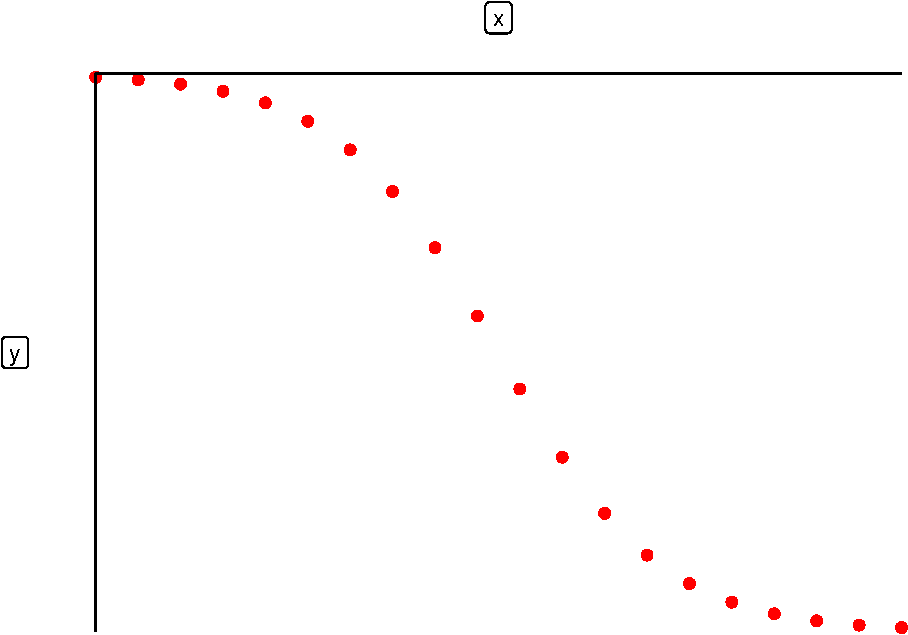
\includegraphics{Introduccion_a_Muestreo_files/figure-latex/unnamed-chunk-143-1.pdf}

\begin{enumerate}
\def\labelenumi{\alph{enumi}.}
\tightlist
\item
  La correlación de Pearson de \(\vec{x}\) y \(\vec{y}\) es \(-1\)

  \begin{itemize}
  \tightlist
  \item
    Verdadero
  \item
    Falso
  \item
    No se puede determinar
  \end{itemize}
\item
  La correlación de Spearman de \(\vec{x}\) y \(\vec{y}\) es \(-1\)

  \begin{itemize}
  \tightlist
  \item
    Verdadero
  \item
    Falso\\
  \item
    No se puede determinar
  \end{itemize}
\item
  La tau de Kendall de \(\vec{x}\) y \(\vec{y}\) es \(-1\)

  \begin{itemize}
  \tightlist
  \item
    Verdadero
  \item
    Falso
  \item
    No se puede determinar
  \end{itemize}
\end{enumerate}

\begin{enumerate}
\def\labelenumi{\arabic{enumi}.}
\setcounter{enumi}{26}
\tightlist
\item
  A partir de la siguiente gráfica determina si los incisos son verdaderos o falsos o no se puede determinar:
\end{enumerate}

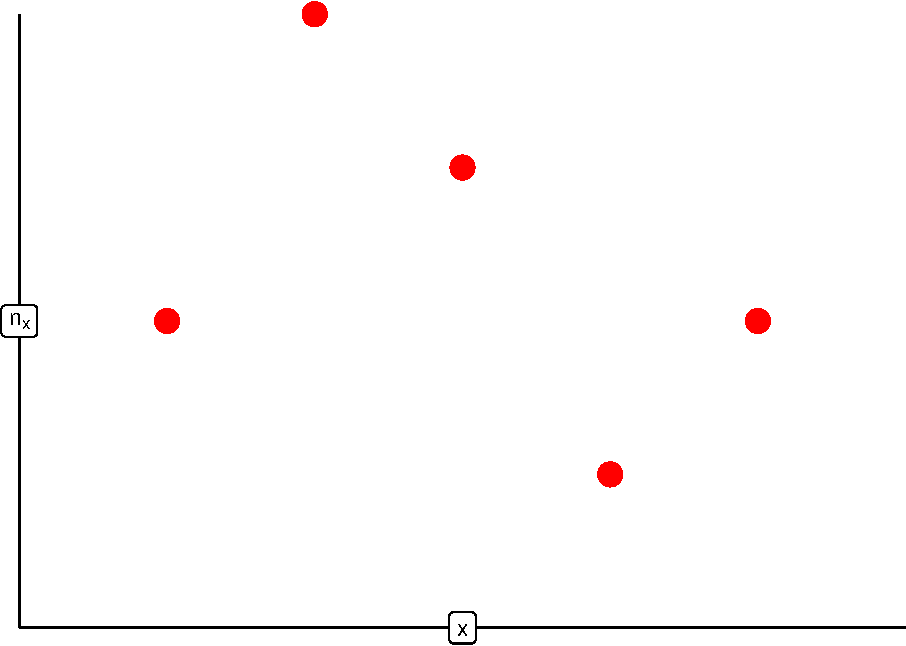
\includegraphics{Introduccion_a_Muestreo_files/figure-latex/unnamed-chunk-144-1.pdf}

\begin{enumerate}
\def\labelenumi{\alph{enumi}.}
\tightlist
\item
  El coeficiente de asimetría de \(\vec{x}\) es positivo.

  \begin{itemize}
  \tightlist
  \item
    Verdadero
  \item
    Falso
  \item
    No se puede determinar
  \end{itemize}
\item
  El coeficiente de curtosis de \(\vec{x}\) es positivo.

  \begin{itemize}
  \tightlist
  \item
    Verdadero
  \item
    Falso
  \item
    No se puede determinar
  \end{itemize}
\item
  La distribución de \(\vec{x}\) tiene una sola moda.

  \begin{itemize}
  \tightlist
  \item
    Verdadero
  \item
    Falso
  \item
    No se puede determinar
  \end{itemize}
\end{enumerate}

\begin{enumerate}
\def\labelenumi{\arabic{enumi}.}
\setcounter{enumi}{27}
\tightlist
\item
  Considera el problema de mínimos cuadrados donde ahora suponemos que existe una submatriz \(X_{n \times k}\) de la base de datos \(Z\) y un vector columna \(y\) tal que cada entrada de las \(y\), \(y_i\) es una función lineal de las \(x_{i,j}\):
  \[
  y_i = \beta_1 x_{i,1} + \beta_2 x_{i,2} + \dots + \beta_k x_{i,k}
  \]
  Suponemos, además que las columnas de \(X_{n \times k}\) son linealmente independientes (\emph{i.e.} es de rango completo). En este caso la función de error a minimizar para estimar las \(\beta\)s es:
  \[
  \text{SSR}(\beta_1, \beta_2, \dots, \beta_k) = \sum\limits_{i=1}^n \big( y_i - \sum\limits_{j=1}^k \beta_j x_{i,j}\big)^2
  \]
\end{enumerate}

\begin{enumerate}
\def\labelenumi{\alph{enumi}.}
\tightlist
\item
  Demuestra que en este caso el problema es equivalente a minimizar:
  \begin{equation}\nonumber
  \text{SSR}(\vec{\beta}) = (\vec{y} - X \vec{\beta})^T (\vec{y} - X \vec{\beta})
  \end{equation}
\item
  Obtén entonces que:
  \begin{equation}\nonumber
  \beta = (X^T X)^{-1} X^T \vec{y}
  \end{equation}\\
\item
  Finalmente, suponiendo que \(y = \alpha + \gamma x + \eta z\) es un hiperplano de \(x\) y \(z\) calcula los coeficientes:
\end{enumerate}

\begin{tabular}{r|r|r}
\hline
x & y & z\\
\hline
1 & 7 & -1\\
\hline
2 & 9 & -2\\
\hline
3 & 12 & -3\\
\hline
1 & 14 & 1\\
\hline
\end{tabular}

\begin{enumerate}
\def\labelenumi{\alph{enumi}.}
\setcounter{enumi}{3}
\tightlist
\item
  Verifica los coeficientes haciendo la regresión en \texttt{R}.
\end{enumerate}

\hypertarget{muestreo-aleatorio-simple}{%
\chapter{Muestreo Aleatorio Simple}\label{muestreo-aleatorio-simple}}

\hypertarget{inicio-1}{%
\section{Inicio}\label{inicio-1}}

Siempre que inicies un nuevo trabajo en \texttt{R} ¡no olvides borrar el historial!

\begin{Shaded}
\begin{Highlighting}[]
\FunctionTok{rm}\NormalTok{(}\AttributeTok{list =} \FunctionTok{ls}\NormalTok{()) }\CommentTok{\#Clear all}
\end{Highlighting}
\end{Shaded}

\hypertarget{libreruxedas-1}{%
\section{Librerías}\label{libreruxedas-1}}

Para este análisis vamos a tener que llamar a las siguientes librerías previamente instaladas (por única vez) con \texttt{install.packages}:

\begin{Shaded}
\begin{Highlighting}[]
\FunctionTok{library}\NormalTok{(tidyverse)}
\FunctionTok{library}\NormalTok{(dplyr)}
\FunctionTok{library}\NormalTok{(imager)}
\FunctionTok{library}\NormalTok{(rlist)}
\FunctionTok{library}\NormalTok{(gridExtra)}
\FunctionTok{library}\NormalTok{(kableExtra)}
\end{Highlighting}
\end{Shaded}

\hypertarget{notaciuxf3n}{%
\section{Notación}\label{notaciuxf3n}}

Supongamos una matriz de datos de tamaño \(N \times L\) dada por:
\[
U = \begin{pmatrix} 
z_1 \Big| z_2 \Big| \dots \Big| z_{\ell}
\end{pmatrix} 
\]

donde las \(z_i\) representan las columnas de la matriz. La \(U\) será conocida como la \textbf{matriz universo} (el \emph{universo} ó \emph{la población}) si contiene \emph{toda} la información de la población. Intuitivamente, la matriz \(U\) son todos los datos de un censo: esta es una matriz \emph{ideal} donde están todos los datos.

A cualquier permutación en las filas de una submatriz \(S\) (tamaño \(n \times \ell\) con \(0 < n \leq N\) y \(0 < \ell \leq L\)) de \(U\) se le conoce como una \emph{muestra} de \(U\). Si \(S\) es una variable aleatoria (por ejemplo, porque se construyó a partir de un mecanismo de aleatoreidad) decimos que \(S\) es una \textbf{muestra aleatoria} (denotamos \(\mathcal{S}\) a la variable aleatoria y \(S\) a un valor específico de la misma).\footnote{En la literatura muchas referencias establecen una muestra aleatoria como un conjunto de valores. Yo utilizo vectores para poder hablar de repeticiones (por ejemplo si extraes el mismo valor varias veces en la muestra).}

En particular en esta sección (y hasta establecer lo contrario) consideraremos que el universo \(U\) es de tamaño \(N \times 1\) y la submatriz \(S\) (resp. \(\mathcal{S}\)) es de tamaño \(n \times 1\). En notación \(U = (x_1, x_2, \dots, x_N)^T\) y \emph{técnicamente} \(S = (x_{i_1}, x_{i_2}, \dots, x_{i_n})^T\) para un conjunto de índices \(i_1, i_2, \dots, i_n\). Sin embargo para simplificar la notación consideraremos que en \(S\) están los primeros \(n\) de los \(x_i\); es decir:
\[
S = (x_1, x_2, \dots, x_n)^T
\]

Cuando estemos hablando de la muestra \emph{como variable aleatoria} \(\mathcal{S}\) y no como \emph{valores observados (fijos)} \(S\), denotaremos:
\[
\mathcal{S} = (X_1, X_2, \dots, X_n)^T
\]
donde \(\mathcal{S}\) representa la muestra posible y cada \(X_i\) es una variable aleatoria con el valor posible de la i-ésima entrada.

Un \textbf{esquema muestral} es una función \(\mathbb{P}\) de probabilidad definida en el conjunto de submatrices de \(U\). Ésta es el punto medular de todas las estrategias de muestreo: distintos esquemas muestrales generan diferentes distribuciones y pueden llevar a distintas inferencias sobre un fenómeno.

\hypertarget{ejemplo}{%
\subsection{Ejemplo}\label{ejemplo}}

Considera la matriz universo con tres letras:
\[
U = \begin{pmatrix}
\text{A} \\
\text{B} \\
\text{C} 
\end{pmatrix}
\]
Ésta es la matriz universo. Las submatrices\footnote{Enumero las submatrices para luego poder hablar de ellas} que pueden crearse a partir de dicho universo son:

\begin{enumerate}
\def\labelenumi{\arabic{enumi}.}
\item
  De dimensión \(n = 1\): \(S^1 = (\text{A})^T\), \(S^2 = (\text{B})^T\), \(S^3 = (\text{C})^T\).
\item
  De dimensión \(n = 2\): \(S^4 = (\text{A}, \text{B})^T\), \(S^5 = (\text{A}, \text{C})^T\), \(S^6 = (\text{B}, \text{C})^T\), \(S^7 = (\text{B}, \text{A})^T\), \(S^8 = (\text{C}, \text{A})^T\), \(S^9 = (\text{C}, \text{B})^T\).
\item
  De dimensión \(n = 3\): \(S^{10} = (\text{A}, \text{B}, \text{C})^T\), \(S^{11} = (\text{B}, \text{A}, \text{C})^T\), \(S^{12} = (\text{A}, \text{C}, \text{B})^T\), \(S^{13} = (\text{C}, \text{B}, \text{A})^T\), \(S^{14} = (\text{B}, \text{C}, \text{A})^T\), \(S^{15} = (\text{C}, \text{A}, \text{B})^T\),
\end{enumerate}

Un esquema muestral sería la función de probabilidad:
\[
\mathbb{P}(\mathcal{S} = S^k) = \begin{cases}
0.1 & \text{ si } k = 1, \\
0.2 & \text{ si } k = 3, \\
0.5 & \text{ si } k = 11, \\
0.2 & \text{ si } k = 15, \\
0   & \text{ en otro caso.}
\end{cases}
\]

Otro esquema muestral posible sería:
\[
\mathbb{P}(\mathcal{S} = S^k) = \begin{cases}
\frac{1}{3} & \text{ si } k = 1, \\
\frac{1}{3} & \text{ si } k = 2, \\
\frac{1}{3} & \text{ si } k = 3, \\
0   & \text{ en otro caso.}
\end{cases}
\]
Este último esquema, intuitivamente, corresponde a la selección aleatoria de un elemento de \(U\) con una probabilidad uniforme de que cada elemento salga.

A fin de simplificar el problema (y hasta que se diga lo contrario) agregaremos la hipótesis de \textbf{intercambiabilidad}; es decir, consideraremos es irrelevante el orden de las filas de las submatrices de datos. Por ejemplo, bajo intercambiabilidad, \(S^4 = (\text{A}, \text{B})^T\) es \emph{la misma matriz} que \(S^7 = (\text{B}, \text{A})^T\).

\begin{quote}
Un ejemplo de muestra donde el orden sí importa (\emph{i.e.} no son intercambiables) es cuando se realizan exámenes orales según una selección aleatoria de la lista. La tercera persona en presentar el examen estará informada por el \emph{¿qué te preguntó el profe?}, \emph{¿estuvo difícil?} que las primeras dos le cuenten.
\end{quote}

Bajo intercambiabilidad, los esquemas muestrales estarán definidos únicamente sobre los siguientes vectores:

\begin{enumerate}
\def\labelenumi{\arabic{enumi}.}
\item
  De dimensión \(n = 1\): \(S^1 = (\text{A})^T\), \(S^2 = (\text{B})^T\), \(S^3 = (\text{C})^T\).
\item
  De dimensión \(n = 2\): \(S^4 = (\text{A}, \text{B})^T\), \(S^5 = (\text{A}, \text{C})^T\), \(S^6 = (\text{B}, \text{C})^T\).
\item
  De dimensión \(n = 3\): \(S^{7} = (\text{A}, \text{B}, \text{C})^T\).
\end{enumerate}

En este caso un esquema muestral sería:
\[
\mathbb{P}(\mathcal{S} = S^k) = \begin{cases}
\frac{1}{16} & \text{ si } k = 1, \\
\frac{3}{16} & \text{ si } k = 2, \\
0 & \text{ si } k = 3, \\
\frac{7}{16} & \text{ si } k = 4, \\
\frac{1}{16} & \text{ si } k = 5, \\
\frac{4}{16} & \text{ si } k = 6, \\
0   & \text{ en otro caso.}
\end{cases}
\]
Dado un elemento \(x_i\) del universo, podemos preguntarnos por la probabilidad de que dicho \(x_i\) esté en la muestra. Siguiendo el ejemplo anterior:
\[
\mathbb{P}(\text{A} \in \mathcal{S}) = \mathbb{P}(\mathcal{S} = S^1) + \mathbb{P}(\mathcal{S} = S^4) + \mathbb{P}(\mathcal{S} = S^5) + \mathbb{P}(\mathcal{S} = S^7) = \frac{9}{16}.
\]

Como notación, para una población \(U = (x_1, x_2, \dots, x_N)^T\) y una muestra aleatoria \(\mathcal{S}\) denotamos la probabilidad de que \(x_k\) esté en la muestra como:
\[
\pi_k = \mathbb{P}(x_k \in \mathcal{S})
\]
Estas probabilidades (para \(k = 1,2,\dots, N\)) se conocen como \textbf{probabilidades de inclusión de primer orden}. La probabilidad conjunta de que \(x_k\) y \(x_l\) (ambos) estén en la muestra (\textbf{probabilidad de inclusión de segundo orden}) está dada por:
\[
\pi_{k,l} = \mathbb{P}(x_k \in \mathcal{S}, x_l \in \mathcal{S})
\]
Notamos que por definición \(\pi_{kk} = \pi_k\). Análogamente se pueden crear probabilidades de inclusión de cualquier orden deseado.

Finalmente, una población \(U = (x_1, x_2, \dots, x_N)^T\) y una muestra aleatoria \(\mathcal{S}\) definimos la variable indicadora de que \(x_k\) esté en la muestra como:
\[
\mathbb{I}_{\mathcal{S}}(x_k) = \begin{cases}
1 & \text{ si } x_k \in \mathcal{S} \\
0 & \text{ si } x_k \not\in \mathcal{S} \\
\end{cases}
\]
Notamos que para una muestra aleatoria \(\mathcal{S}\) las indicadoras tienen una distribución conocida:
\[
\mathbb{I}_{\mathcal{S}}(x_k) \sim \text{Bernoulli}(\pi_k)
\]
pues
\[
\mathbb{P}\big( \mathbb{I}_{\mathcal{S}}(x_k)  = 1\big) = \mathbb{P}\big(x_k \in \mathcal{S}) = \pi_k
\]
Como las \(\mathbb{I}_{\mathcal{S}}(x_k)\) son Bernoulli podemos \href{https://en.wikipedia.org/wiki/Bernoulli_distribution}{calcular su varianza}:
\[
\text{Var}\Big( \mathbb{I}_{\mathcal{S}}(x_k)\Big) = \pi_k (1 - \pi_k)
\]
Finalmente, recordamos que la covarianza entre dos variables aleatorias \(X\), \(Y\) se define como:
\[
\text{Cov}(X,Y) = \mathbb{E}[XY] - \mathbb{E}[X]\cdot\mathbb{E}[Y]
\]
Por lo que calculamos la covarianza entre dos indicadoras (de \(x_k\) y \(x_l\)):
\begin{equation}
\begin{aligned}
\text{Cov}\Big(\mathbb{I}_{\mathcal{S}}(x_k), \mathbb{I}_{\mathcal{S}}(x_l) \Big) & = \mathbb{E}\Big[\mathbb{I}_{\mathcal{S}}(x_k) \cdot \mathbb{I}_{\mathcal{S}}(x_l)\Big] -   \mathbb{E}\Big[\mathbb{I}_{\mathcal{S}}(x_k)\Big] \mathbb{E}\Big[\mathbb{I}_{\mathcal{S}}(x_l)\Big]
\\ & = 1 \cdot \mathbb{P}\Big( \mathbb{I}_{\mathcal{S}}(x_k) \cdot \mathbb{I}_{\mathcal{S}}(x_l) = 1) + 0 \cdot \mathbb{P}\Big( \mathbb{I}_{\mathcal{S}}(x_k) \cdot \mathbb{I}_{\mathcal{S}}(x_l) = 0) - \pi_k \pi_l \\
& = \mathbb{P}\Big( \mathbb{I}_{\mathcal{S}}(x_k)  = 1, \mathbb{I}_{\mathcal{S}}(x_l) = 1) - \pi_k \pi_l \\
& = \pi_{k,l} -\pi_k \pi_l
\end{aligned}
\end{equation}
La cantidad \(\pi_{k,l} -\pi_k \pi_l\) usualmente se denota \(\Delta_{k,l}\):
\[
\Delta_{k,l} = \pi_{k,l} -\pi_k \pi_l
\]

A continuación hablaremos de algunos esquemas de muestreo comunmente utilizados y, finalmente, llegaremos a una generalización de los mismos.

\hypertarget{ejercicio-5}{%
\subsection{Ejercicio}\label{ejercicio-5}}

Demuestra las siguientes propiedades de los \(\pi_k\) para un diseño muestral \(\mathbb{P}\) con tamaño fijo de la muestra \(n\in\mathbb{N}\):

\begin{enumerate}
\def\labelenumi{\arabic{enumi}.}
\item
  \(\sum\limits_{k=1}^N \pi_k = n\)
\item
  \(\sum\limits_{\substack{k=1 \\\\ k \neq l}}^N \sum\limits_{l=1}^N \pi_{k,l} = n(n-1)\)
\item
  \(\sum\limits_{\substack{l=1 \\\\ l \neq k}}^N \pi_{k,l} = (n-1) \pi_k\)
\end{enumerate}

\hypertarget{muestreo-aleatorio-simple-sin-reemplazo-massr}{%
\section{Muestreo Aleatorio Simple sin Reemplazo (MAS/sR)}\label{muestreo-aleatorio-simple-sin-reemplazo-massr}}

Vamos a considerar una de las formas más sencillas de muestreo: el aleatorio simple \emph{sin reemplazo} . Para ello seleccionamos de \(U = (x_1, x_2, \dots, x_N)^T\) a \(n\in\mathbb{N}\) (fijo) observaciones asignándole la probabilidad de ser seleccionada a cada una de \(\frac{1}{N}\). Una vez se selecciona la primera, se selecciona una de las que restan de \(U\) con probabilidad \(\frac{1}{N-1}\). El proceso se repite hasta extraer \(n\) elementos.

Comencemos por un ejemplo, supongamos tenemos una población de cinco personas:
\[
U = \Big( \text{Ana}, \text{Beto}, \text{Carlos}, \text{Diana}, \text{Enriqueta}\Big)^T
\]
Si queremos tomar una muestra de \(3\) personas sin reemplazo, las muestras posibles son:

\begin{enumerate}
\def\labelenumi{\arabic{enumi}.}
\item
  \(\Big( \text{Ana}, \text{Beto}, \text{Carlos}\Big)^T\)
\item
  \(\Big( \text{Ana}, \text{Carlos}, \text{Diana}\Big)^T\)
\item
  \(\Big( \text{Ana}, \text{Beto}, \text{Diana}\Big)^T\)
\item
  \(\Big( \text{Ana}, \text{Beto}, \text{Enriqueta}\Big)^T\)
\item
  \(\Big( \text{Ana}, \text{Carlos}, \text{Enriqueta}\Big)^T\)
\item
  \(\Big( \text{Ana}, \text{Diana}, \text{Enriqueta}\Big)^T\)
\item
  \(\Big( \text{Beto}, \text{Carlos}, \text{Diana}\Big)^T\)
\item
  \(\Big( \text{Beto}, \text{Diana}, \text{Enriqueta}\Big)^T\)
\item
  \(\Big( \text{Beto}, \text{Carlos}, \text{Enriqueta}\Big)^T\)
\item
  \(\Big( \text{Carlos}, \text{Diana}, \text{Enriqueta}\Big)^T\)
\end{enumerate}

Obtener una muestra aleatoria se puede hacer en \texttt{R} con un vector mediante \texttt{sample}:

\begin{Shaded}
\begin{Highlighting}[]
\CommentTok{\#Vector de nombres}
\NormalTok{nombres }\OtherTok{\textless{}{-}} \FunctionTok{c}\NormalTok{(}\StringTok{"Ana"}\NormalTok{,}\StringTok{"Beto"}\NormalTok{,}\StringTok{"Carlos"}\NormalTok{,}\StringTok{"Diana"}\NormalTok{,}\StringTok{"Enriqueta"}\NormalTok{)}

\CommentTok{\#Muestra}
\FunctionTok{sample}\NormalTok{(nombres, }\DecValTok{3}\NormalTok{, }\AttributeTok{replace =} \ConstantTok{FALSE}\NormalTok{)}
\end{Highlighting}
\end{Shaded}

\begin{verbatim}
## [1] "Beto"  "Ana"   "Diana"
\end{verbatim}

Formalmente, un esquema de muestreo es \textbf{aleatorio simple sin reemplazo} si dada una constante \(n \in \mathbb{N}\) (con \(0 < n \leq N\)) se tiene:

\[
\mathbb{P}\big( \mathcal{S} = S \big) = \begin{cases}
\frac{1}{\binom{N}{n}} & \text{ si } \#S = n \\
0 & \text{ en otro caso.}
\end{cases}
\]
En el caso de muestreo aleatorio simple sin reemplazo podemos calcular las probabilidades de inclusión como siguen:
\[
\pi_k = \mathbb{P}(x_k \in \mathcal{S}) = \sum\limits_{i=1}^{M_1} \frac{1}{\binom{N}{n}} = \frac{\binom{N-1}{n-1}}{\binom{N}{n}} = \frac{n}{N} = f
\]
donde la tercera igualdad se sigue de que hay \(M_1 = \binom{N-1}{n-1}\) muestras que contienen al \(x_k\). (La lógica es, fijo el \(x_k\) y entonces me quedan \(N-1\) valores de \(x\) a acomodar en \(n-1\) espacios). Por otro lado:
\[
\pi_{k,j} = \mathbb{P}(x_k \in \mathcal{S}, x_j \in S) = \sum\limits_{i=1}^{M_2}  \frac{1}{\binom{N}{n}} = \frac{\binom{N-2}{n-2}}{\binom{N}{n}} = \dfrac{n(n-1)}{N(N-1)}
\]
pues hay \(M_2 = \binom{N-2}{n-2}\) muestras conteniendo a \(x_k\) y \(x_j\) a la vez.

Para estimar el total poblacional dado por:
\[
t = \sum\limits_{i=1}^N x_i
\]
bajo \emph{MAS/sR} podemos tomar:
\[
\hat{t} = N \cdot \bar{x}_{\mathcal{S}} = N \frac{1}{n} \sum\limits_{k = 1}^n x_k=  \sum\limits_{k = 1}^n \dfrac{x_k}{n/N} =  
\sum\limits_{k=1}^N \frac{x_k}{\pi_k} \cdot \mathbb{I}_{\mathcal{S}}(x_k)
\]
Notamos entonces que el estimador \(\hat{t}\) es una variable aleatoria pues depende de las indicadoras de la muestra. En particular:
\[
\mathbb{E}\big[ \hat{t} \big] = \mathbb{E}\bigg[\sum\limits_{k=1}^N \frac{x_k}{\pi_k} \cdot \mathbb{I}_{\mathcal{S}}(x_k) \bigg] = \sum\limits_{k=1}^N \frac{x_k}{\pi_k} \underbrace{\mathbb{E}\bigg[\mathbb{I}_{\mathcal{S}}(x_k) \bigg]}_{\pi_k}  = t
\]
de donde se sigue que en promedio el estimador \(\hat{t}\) vale el total.

\textbf{Definición: {[}Insesgado{]}} Un estimador \(\hat{\theta}\) es un estimador insesgado de \(\theta\) si:
\[
\mathbb{E}\big[ \hat{\theta} - \theta] = 0
\]
En nuestro caso \(\hat{t}\) es \emph{insesgado}. En general, la cantidad \(\mathbb{E}\big[ \hat{\theta} - \theta]\) se conoce como \emph{el sesgo} .

De manera numérica, podemos simular la estimación del total en \texttt{1000} simulaciones como sigue:

\begin{Shaded}
\begin{Highlighting}[]
\NormalTok{nsim }\OtherTok{\textless{}{-}} \DecValTok{1000}
\NormalTok{N    }\OtherTok{\textless{}{-}} \DecValTok{1000}
\NormalTok{n    }\OtherTok{\textless{}{-}} \DecValTok{100} 
\NormalTok{base.completa }\OtherTok{\textless{}{-}} \FunctionTok{data.frame}\NormalTok{(}\AttributeTok{x =} \FunctionTok{rnorm}\NormalTok{(N))}
\NormalTok{total         }\OtherTok{\textless{}{-}} \FunctionTok{sum}\NormalTok{(base.completa}\SpecialCharTok{$}\NormalTok{x)}
\NormalTok{total.muestra }\OtherTok{\textless{}{-}} \FunctionTok{rep}\NormalTok{(}\ConstantTok{NA}\NormalTok{, nsim)}
\ControlFlowTok{for}\NormalTok{ (i }\ControlFlowTok{in} \DecValTok{1}\SpecialCharTok{:}\NormalTok{nsim)\{}
\NormalTok{  muestra          }\OtherTok{\textless{}{-}} \FunctionTok{sample}\NormalTok{(base.completa}\SpecialCharTok{$}\NormalTok{x, n)}
\NormalTok{  total.muestra[i] }\OtherTok{\textless{}{-}}\NormalTok{ N}\SpecialCharTok{*}\FunctionTok{mean}\NormalTok{(muestra)}
\NormalTok{\}}
\FunctionTok{mean}\NormalTok{(total.muestra)}
\end{Highlighting}
\end{Shaded}

\begin{verbatim}
## [1] -78.75412
\end{verbatim}

Podemos ver las simulaciones como sigue:

\begin{Shaded}
\begin{Highlighting}[]
\FunctionTok{ggplot}\NormalTok{() }\SpecialCharTok{+}
  \FunctionTok{geom\_histogram}\NormalTok{(}\FunctionTok{aes}\NormalTok{(}\AttributeTok{x =}\NormalTok{ total.muestra, }\AttributeTok{y =}\NormalTok{ ..density..), }\AttributeTok{fill =} \StringTok{"\#008B8B"}\NormalTok{, }
                 \AttributeTok{color =} \StringTok{"white"}\NormalTok{, }\AttributeTok{binwidth =} \DecValTok{40}\NormalTok{) }\SpecialCharTok{+} 
  \FunctionTok{geom\_vline}\NormalTok{(}\FunctionTok{aes}\NormalTok{(}\AttributeTok{xintercept =}\NormalTok{ total), }\AttributeTok{linetype =} \StringTok{"dashed"}\NormalTok{) }\SpecialCharTok{+}
  \FunctionTok{theme\_classic}\NormalTok{() }
\end{Highlighting}
\end{Shaded}

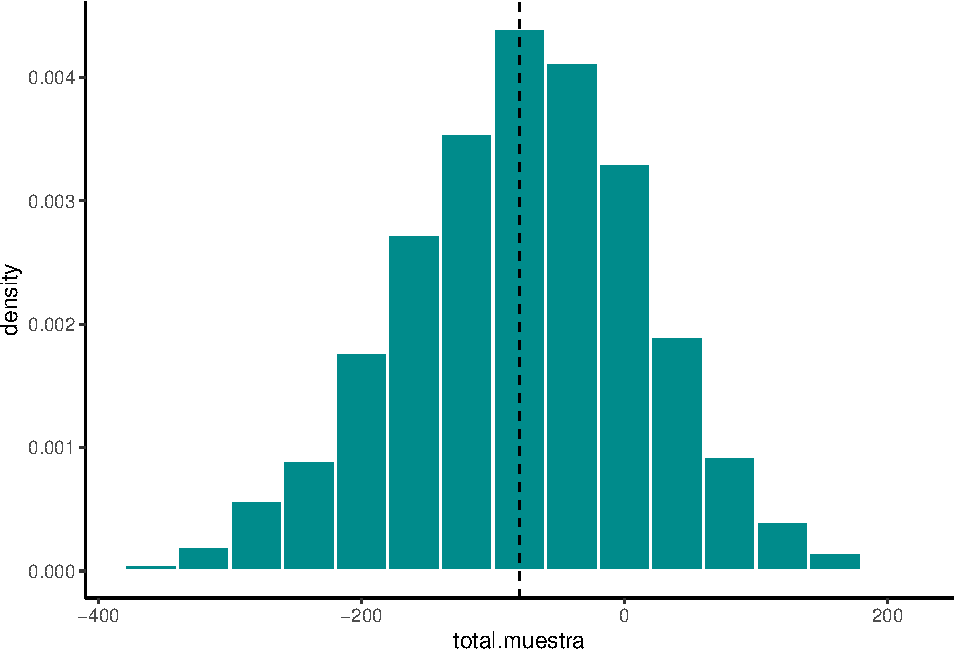
\includegraphics{Introduccion_a_Muestreo_files/figure-latex/unnamed-chunk-150-1.pdf}

Como podrás notar la \(\hat{t}\) es una variable aleatoria y por tanto tiene varianza. De hecho:
\[
\textrm{Var}(\hat{t}) = \sum\limits_{k = 1}^N \sum\limits_{l = 1}^N \Delta_{k,l} \frac{x_k}{\pi_k} \frac{x_l}{\pi_l}
\]
Para demostrarlo seguimos las igualdades:
\begin{equation}\nonumber
\begin{aligned}
\textrm{Var}(\hat{t})  & = \textrm{Var}\Bigg( \sum\limits_{k=1}^N \frac{x_k}{\pi_k} \cdot \mathbb{I}_{\mathcal{S}}(x_k) \Bigg)
\\ & = \sum\limits_{k=1}^N  \frac{x_k^2}{\pi_k^2} \cdot \textrm{Var}\Big(\mathbb{I}_{\mathcal{S}}(x_k) \Big) + \sum\limits_{k = 1}^N \sum\limits_{\substack{l = 1 \\ \\ l \neq k}}^{N}  \frac{x_k}{\pi_k}  \frac{x_l}{\pi_l} \cdot \textrm{Cov}\Big(\mathbb{I}_{\mathcal{S}}(x_k), \mathbb{I}_{\mathcal{S}}(x_l) \Big)
\\ & = \sum\limits_{k=1}^N  \frac{x_k^2}{\pi_k^2} \cdot \underbrace{\pi_k (1 - \pi_k)}_{\Delta_{k,k}} + \sum\limits_{k = 1}^N \sum\limits_{\substack{l = 1 \\ \\ l \neq k}}^{N} \frac{x_k}{\pi_k}  \frac{x_l}{\pi_l} \cdot \underbrace{\textrm{Cov}\Big(\mathbb{I}_{\mathcal{S}}(x_k), \mathbb{I}_{\mathcal{S}}(x_l) \Big)}_{\Delta_{k,l}}
\\ & = \sum\limits_{k = 1}^N \sum\limits_{\substack{l = 1 \\ \\ l \neq k}}^{N}\Delta_{k,l} \frac{x_k}{\pi_k} \frac{x_l}{\pi_l}
\end{aligned}
\end{equation}

Numéricamente, en el ejemplo anterior la varianza (simulada) de \(\hat{t}\) es:

\begin{Shaded}
\begin{Highlighting}[]
\FunctionTok{var}\NormalTok{(total.muestra)}
\end{Highlighting}
\end{Shaded}

\begin{verbatim}
## [1] 8515.982
\end{verbatim}

mientras que la \emph{real} está dada por (ver ejercicio más adelante):

\begin{Shaded}
\begin{Highlighting}[]
\NormalTok{f        }\OtherTok{\textless{}{-}}\NormalTok{ n}\SpecialCharTok{/}\NormalTok{N}
\NormalTok{varianza }\OtherTok{\textless{}{-}}\NormalTok{ N}\SpecialCharTok{\^{}}\DecValTok{2}\SpecialCharTok{*}\NormalTok{(}\DecValTok{1} \SpecialCharTok{{-}}\NormalTok{ f)}\SpecialCharTok{/}\NormalTok{n}\SpecialCharTok{*}\FunctionTok{var}\NormalTok{(base.completa}\SpecialCharTok{$}\NormalTok{x)}
\FunctionTok{print}\NormalTok{(varianza)}
\end{Highlighting}
\end{Shaded}

\begin{verbatim}
## [1] 8278.693
\end{verbatim}

Nota que tenemos un problema: para estimar \(\textrm{Var}(\hat{t})\) necesitamos conocer todas las \(x_k\) de la población ¡lo cual es imposible! Entonces necesitamos un estimador de la varianza de \(\hat{t}\) para lo cual proponemos:

\[
\widehat{\textrm{Var}}(\hat{t}) = \sum\limits_{k = 1}^n \sum\limits_{l = 1}^n \dfrac{\Delta_{k,l}}{\pi_{k,l}} \frac{x_k}{\pi_k} \frac{x_l}{\pi_l}
\]

Para demostrar que el estimador es insesgado tomamos el valor esperado y agregamos las variables indicadoras correspondientes:

\[
\widehat{\textrm{Var}}(\hat{t})  = \sum\limits_{k = 1}^N \sum\limits_{l = 1}^N \dfrac{\Delta_{k,l}}{\pi_{k,l}} \frac{x_k}{\pi_k} \frac{x_l}{\pi_l} \mathbb{I}_{\mathcal{S}}(x_k) \mathbb{I}_{\mathcal{S}}(x_l) 
\]
Se sigue la demostración:

\begin{equation}\nonumber
\begin{aligned}
\mathbb{E}\Big[\widehat{\textrm{Var}}(\hat{t})  \Big] & = \mathbb{E}\bigg[ \sum\limits_{k = 1}^N \sum\limits_{l = 1}^N \dfrac{\Delta_{k,l}}{\pi_{k,l}} \frac{x_k}{\pi_k} \frac{x_l}{\pi_l} \mathbb{I}_{\mathcal{S}}(x_k) \mathbb{I}_{\mathcal{S}}(x_l) \bigg] \\
& = \sum\limits_{k = 1}^N \sum\limits_{l = 1}^N \dfrac{\Delta_{k,l}}{\pi_{k,l}} \frac{x_k}{\pi_k} \frac{x_l}{\pi_l} \underbrace{\mathbb{E}\bigg[  \mathbb{I}_{\mathcal{S}}(x_k) \mathbb{I}_{\mathcal{S}}(x_l) \bigg]}_{*} \\
\end{aligned}
\end{equation}
donde notamos que:

\begin{equation}\nonumber
\begin{aligned}
* = \mathbb{E}\bigg[  \mathbb{I}_{\mathcal{S}}(x_k) \mathbb{I}_{\mathcal{S}}(x_l) \bigg] & = \textrm{Cov}\Big( \mathbb{I}_{\mathcal{S}}(x_k), \mathbb{I}_{\mathcal{S}}(x_l) \Big) + \mathbb{E}\Big[ \mathbb{I}_{\mathcal{S}}(x_k)\Big] \mathbb{E}\Big[ \mathbb{I}_{\mathcal{S}}(x_l)\Big] \\ & = \pi_{k,l} - \pi_k \pi_l + \pi_k\pi_l 
\\ & = \pi_{k,l}
\end{aligned}
\end{equation}

de donde se sigue:

\begin{equation}\nonumber
\begin{aligned}
\mathbb{E}\Big[\widehat{\textrm{Var}}(\hat{t})  \Big] & = \sum\limits_{k = 1}^N \sum\limits_{l = 1}^N \dfrac{\Delta_{k,l}}{\pi_{k,l}} \frac{x_k}{\pi_k} \frac{x_l}{\pi_l}\underbrace{ \pi_{k,l}}_{*} 
\\ & = \sum\limits_{k = 1}^N \sum\limits_{l = 1}^N \Delta_{k,l} \frac{x_k}{\pi_k} \frac{x_l}{\pi_l} = \textrm{Var}(\hat{t})
\end{aligned}
\end{equation}

Podemos calcular la varianza estimada para una muestra aleatoria simple sin reemplazo como sigue (ver ejercicio):

\begin{Shaded}
\begin{Highlighting}[]
\NormalTok{f        }\OtherTok{\textless{}{-}}\NormalTok{ n}\SpecialCharTok{/}\NormalTok{N}
\NormalTok{varianza }\OtherTok{\textless{}{-}}\NormalTok{ N}\SpecialCharTok{\^{}}\DecValTok{2}\SpecialCharTok{*}\NormalTok{(}\DecValTok{1} \SpecialCharTok{{-}}\NormalTok{ f)}\SpecialCharTok{/}\NormalTok{n}\SpecialCharTok{*}\FunctionTok{var}\NormalTok{(muestra)}
\FunctionTok{print}\NormalTok{(varianza)}
\end{Highlighting}
\end{Shaded}

\begin{verbatim}
## [1] 7811.204
\end{verbatim}

\emph{Observaciones}

\begin{enumerate}
\def\labelenumi{\arabic{enumi}.}
\item
  La media muestral \(\bar{x}_{\mathcal{S}} = \frac{1}{n}\sum\limits_{i = 1}^{n} x_i\) es un estimador insesgado de la media poblacional \(\bar{x}_{\mathcal{U}} = \frac{1}{N}\sum\limits_{i = 1}^{N} x_i\). Se sigue de una factorización de \(n\) del total (\(t\) y \(\hat{t}\) respectivamente).
\item
  Se puede obtener \(\textrm{Var}(\bar{x}_{\mathcal{S}})\) y \(\widehat{\textrm{Var}}(\bar{x}_{\mathcal{S}})\) factorizando las \(n\) de manera cuadrática del \(\hat{t}\).
\end{enumerate}

\hypertarget{ejercicio-6}{%
\subsection{Ejercicio}\label{ejercicio-6}}

Definimos:
\[
s_{x,\mathcal{U}}^2 = \dfrac{1}{N-1} \sum\limits_{k = 1}^N \big( x_k - \bar{x}_{\mathcal{U}})^2
\]
como la \textbf{varianza poblacional ajustada} y
\[
s_{x,\mathcal{S}}^2 = \dfrac{1}{n-1} \sum\limits_{k = 1}^n \big( x_k - \bar{x}_{\mathcal{S}})^2
\]
como la \textbf{varianza muestral ajustada}. Sea \(f = \frac{n}{N}\) la \textbf{fracción muestral}. Demuestra que en el caso de muestreo aleatorio simple sin reemplazo:
\[
\textrm{Var}(\hat{t}) = N^2\dfrac{1-f}{n} s^2_{x,\mathcal{U}}
\]
mientras que el estimador insesgado se transforma en:
\[
\widehat{\textrm{Var}}(\hat{t}) = N^2\dfrac{1-f}{n} s^2_{x,\mathcal{S}}
\]

\hypertarget{teorema-del-luxedmite-central-aplicaciuxf3n}{%
\section{Teorema del Límite Central (Aplicación)}\label{teorema-del-luxedmite-central-aplicaciuxf3n}}

En esta sección hablaremos del teorema central del límite correspondiente a muestreo aleatorio simple con poblaciones finitas. Éste no es el mismo que el de Proba 2 (en términos de hipótesis) aunque las conclusiones sean las mismas. El teorema de Proba 2 establece que si se tiene una colección \(\{ X_i \}\) de variables aleatorias independientes idénticamente distribuidas (todas con distribución acumulada \(F_X\)) con media \(\mu\) y varianza \(\sigma^2 < \infty\), entonces, si definimos \(Z\) como:

\[
Z =\lim_{n \to \infty} \sqrt{\dfrac{n}{\sigma^2}} \cdot  \Big( \frac{1}{n}\sum_{i = 1}^n X_i - \mu\Big)
\]
se tiene que \(Z \sim \textrm{Normal}(0,1)\).

En este teorema central podemos observar que hay algo muy parecido a la media muestral embebido en el teorema (la \(\frac{1}{n}\sum_{i = 1}^n X_i\)) \emph{pero} no es exactamente la media muestral (aquí se supone que todas las \(X_i\) son independientes con distribución \(F_X\) y en el caso de muestreo aleatorio sin reemplazo se sabe que las indicadoras \textbf{NO} son independientes y que de hecho tampoco son idénticamente distribuidas cuando analizamos \(\sum_{i = 1}^{n} x_i \mathbb{I}_{\mathcal{S}}(x_i)\)). Entonces \emph{técnicamente} no podemos aplicar el teorema central del límite así como está a nuestra muestra. Sin embargo, Hàjek (y más tarde \href{https://projecteuclid.org/download/pdf_1/euclid.afm/1485893466}{Rosen} ) encontraron condiciones \emph{sin tener que pedir independencia ni distribución idéntica} que permiten sustituir las \(X_i\) por las de la media muestral (\(x_i \mathbb{I}_{\mathcal{S}}(x_i)\)) y que, cuando \(N\) y \(n\) tienden a infinito ``de buena manera,'' se tiene algo similar a esta expresión (\textbf{OJO} no es una expresión \emph{correcta} pero es la idea):

\[
Z =\lim_{N, n \to \infty} \sqrt{\frac{1}{\textrm{Var}(\bar{x}_{\mathcal{S}})}} \cdot  \Big( \frac{1}{n}\sum_{i = 1}^N x_i \mathbb{I}_{\mathcal{S}}(x_i) - \bar{x}_{\mathcal{U}}\Big)
\]
donde \(\mu = \sum_{k = 1}^N x_k\) es la media poblacional y \(\sigma^2 = \frac{1}{N} \sum_{k = 1}^N (x_k - \mu)^2\) la varianza poblacional no ajustada. La demostración propia de este teorema la posponemos para una sección posterior. Por ahora, ejemplificaremos el teorema del límite central en \texttt{R}, utilizaremos la expresión anterior para deducir y explicar el concepto de intervalo de confianza y, finalmente, haremos un ejemplo de estimación de intervalo.

\hypertarget{estimaciuxf3n-de-intervalos-de-confianza-para-el-total}{%
\subsection{Estimación de intervalos de confianza para el total}\label{estimaciuxf3n-de-intervalos-de-confianza-para-el-total}}

Un intervalo de confianza de \((1 - \alpha)\times 100 \%\) de un estimador poblacional desconocido \(\theta = \theta(x_1, x_2, \dots, x_N)\) (constante) es un intervalo aleatorio de la forma \(\big[ L(\mathcal{S}), U(\mathcal{S}) \big]\) (donde \(L, U\) son variables aleatorias que dependen de la muestra) tal que
\[
\mathbb{P}\Big( \theta \in \big[ L(\mathcal{S}), U(\mathcal{S}) \big]\Big) = 1 - \alpha
\]
Notamos que lo aleatorio del intervalo son las cotas del mismo y que, dadas distintas muestras \(\mathcal{S}\) el valor de interés \(\theta\) no siempre va a caer ahí. La idea de un intervalo es poder dar una cota de más o menos dónde anda un valor. Veamos un ejemplo con el total.

Recordamos que el estimador del total es insesgado \(\mathbb{E}\big[ \hat{t} \big] = t\) y que por definición:
\[
\hat{t} = N \frac{1}{n}\sum\limits_{i = 1}^N x_i \cdot \mathbb{I}_{\mathcal{S}}(x_i) 
\]

luego usando la versión de muestreo finito del teorema central del límite (factorizando \(N\)) tenemos que:

\[
\sqrt{\frac{1}{\textrm{Var}(\bar{x}_{\mathcal{S}})}} \cdot  \Big( \frac{1}{n}\sum_{i = 1}^N x_i \mathbb{I}_{\mathcal{S}}(x_i) - \bar{x}_{\mathcal{U}}\Big) = 
 \cdot  N\dfrac{\Big( \frac{1}{n}\sum_{i = 1}^N x_i \mathbb{I}_{\mathcal{S}}(x_i) - \bar{x}_{\mathcal{U}}\Big)}{N\sqrt{\textrm{Var}(\bar{x}_{\mathcal{S}})}}
=  \dfrac{\hat{t} - t}{\sqrt{\textrm{Var}(\hat{t})}}  \mathrel{\dot\sim} \textrm{Normal}(0,1)
\]
De donde se sigue que si se desea tener un intervalo de tamali \((1 - \alpha) \times 100 \%\) lo que hay que hacer es buscar \(L(\mathcal{S})\) y \(U(\mathcal{S})\) tales que:

\[
\mathbb{P}\Bigg( L(\mathcal{S}) \leq \dfrac{\hat{t} - t}{\sqrt{\textrm{Var}(\hat{t})}} \leq U(\mathcal{S}) \Bigg) = 1 - \alpha
\]
En este caso las probabilidades (por aproximación asintótica) se modelan bajo la hipótesis de normalidad. Y tomamos ventaja de que la normal es simétrica respecto a la media para proponer que \(L(\mathcal{S}) = -U(\mathcal{S})\) y ambas correspondan a \(\pm \Phi^{-1}(\alpha/2)\) (la función de distirbución acumulada inversa de la normal). Es decir, ambos deben corresponder a los cuantiles con probabilidad \(\alpha/2\) y \(1 - \alpha/2\), denotados \(z_{\alpha/2}\) y \(z_{1 - \alpha/2}\). Por simetría de la normal tenemos que: \(z_{\alpha/2} = - z_{1 - \alpha/2}\) y por tanto:
\[
\mathbb{P}\Bigg( z_{\alpha/2} \leq \dfrac{\hat{t} - t}{\sqrt{\textrm{Var}(\hat{t})}} \leq  z_{1 -\alpha/2} \Bigg) = 1 - \alpha
\]
de donde despejamos:
\[
\mathbb{P}\Bigg( z_{\alpha/2}\sqrt{\textrm{Var}(\hat{t})} \leq \hat{t} - t \leq z_{1- \alpha/2}\sqrt{\textrm{Var}(\hat{t})} \Bigg) = \mathbb{P}\Bigg( \hat{t} - z_{1-\alpha/2}\sqrt{\textrm{Var}(\hat{t})} \leq t \leq \hat{t} +  z_{ \alpha/2}\sqrt{\textrm{Var}(\hat{t})} \Bigg)  =  1 - \alpha
\]

Notamos que como no conocemos \(\textrm{Var}(\hat{t})\) la podemos aproximar mediante \(\widehat{\textrm{Var}}(\hat{t})\) (hay mejores aproximaciones mediante una \(t\) de Student asintótica pero no lo usaremos ahora) y tener intervalos aproximados de la forma:
\begin{equation}
\begin{aligned}
L(\mathcal{S}) & =  \hat{t} - z_{1-\alpha/2}\sqrt{\widehat{\textrm{Var}}(\hat{t})} \\
U(\mathcal{S}) & =  \hat{t} + z_{1-\alpha/2}\sqrt{\widehat{\textrm{Var}}(\hat{t})}
\end{aligned}
\end{equation}
de manera concisa muchas veces los escribimos como:
\[
 \hat{t} \pm z_{1-\alpha/2}\sqrt{\widehat{\textrm{Var}}(\hat{t})}
\]

\hypertarget{ejemplo-con-simulaciuxf3n}{%
\subsection{Ejemplo con simulación:}\label{ejemplo-con-simulaciuxf3n}}

Veamos cómo se ven múltiples intervalos simulados con confianza del \(90\%\) y suponiendo la varianza es conocida

\begin{Shaded}
\begin{Highlighting}[]
\NormalTok{nsim }\OtherTok{\textless{}{-}} \DecValTok{100}
\NormalTok{n    }\OtherTok{\textless{}{-}} \DecValTok{100}

\NormalTok{total.muestra  }\OtherTok{\textless{}{-}} \FunctionTok{rep}\NormalTok{(}\ConstantTok{NA}\NormalTok{, nsim)}
\NormalTok{confianza.bajo }\OtherTok{\textless{}{-}} \FunctionTok{rep}\NormalTok{(}\ConstantTok{NA}\NormalTok{, nsim)}
\NormalTok{confianza.alto }\OtherTok{\textless{}{-}} \FunctionTok{rep}\NormalTok{(}\ConstantTok{NA}\NormalTok{, nsim)}
\NormalTok{f }\OtherTok{\textless{}{-}}\NormalTok{ n}\SpecialCharTok{/}\NormalTok{N}
\NormalTok{z }\OtherTok{\textless{}{-}} \FunctionTok{qnorm}\NormalTok{(}\DecValTok{1} \SpecialCharTok{{-}} \FloatTok{0.1}\SpecialCharTok{/}\DecValTok{2}\NormalTok{)}

\NormalTok{var.total      }\OtherTok{\textless{}{-}}\NormalTok{ N}\SpecialCharTok{\^{}}\DecValTok{2}\SpecialCharTok{*}\NormalTok{(}\DecValTok{1} \SpecialCharTok{{-}}\NormalTok{ f)}\SpecialCharTok{/}\NormalTok{n}\SpecialCharTok{*}\FunctionTok{var}\NormalTok{(base.completa}\SpecialCharTok{$}\NormalTok{x)}

  
\ControlFlowTok{for}\NormalTok{ (i }\ControlFlowTok{in} \DecValTok{1}\SpecialCharTok{:}\NormalTok{nsim)\{}
\NormalTok{  muestra           }\OtherTok{\textless{}{-}} \FunctionTok{sample}\NormalTok{(base.completa}\SpecialCharTok{$}\NormalTok{x, n, }\AttributeTok{replace =} \ConstantTok{FALSE}\NormalTok{)}
\NormalTok{  total.muestra[i]  }\OtherTok{\textless{}{-}}\NormalTok{ N}\SpecialCharTok{*}\FunctionTok{mean}\NormalTok{(muestra)}
  \CommentTok{\#var.total[i]    \textless{}{-} N\^{}2*(1 {-} f)/n*var(muestra)}
\NormalTok{  confianza.bajo[i] }\OtherTok{\textless{}{-}}\NormalTok{ total.muestra[i] }\SpecialCharTok{{-}}\NormalTok{ z}\SpecialCharTok{*}\FunctionTok{sqrt}\NormalTok{(var.total)}
\NormalTok{  confianza.alto[i] }\OtherTok{\textless{}{-}}\NormalTok{ total.muestra[i] }\SpecialCharTok{+}\NormalTok{ z}\SpecialCharTok{*}\FunctionTok{sqrt}\NormalTok{(var.total)}
\NormalTok{\}}

\NormalTok{intervalos.simulados }\OtherTok{\textless{}{-}} \FunctionTok{data.frame}\NormalTok{(}
  \AttributeTok{Simulacion =} \DecValTok{1}\SpecialCharTok{:}\NormalTok{nsim,}
  \AttributeTok{Intervalo.Bajo =}\NormalTok{ confianza.bajo,}
  \AttributeTok{Total.Estimado =}\NormalTok{ total.muestra,}
  \AttributeTok{Intervalo.Alto =}\NormalTok{ confianza.alto}
\NormalTok{)}

\FunctionTok{ggplot}\NormalTok{(intervalos.simulados) }\SpecialCharTok{+}
  \FunctionTok{geom\_point}\NormalTok{(}\FunctionTok{aes}\NormalTok{(}\AttributeTok{x =}\NormalTok{ Simulacion, }\AttributeTok{y =}\NormalTok{ Total.Estimado)) }\SpecialCharTok{+}
  \FunctionTok{geom\_errorbar}\NormalTok{(}\FunctionTok{aes}\NormalTok{(}\AttributeTok{x =}\NormalTok{ Simulacion, }\AttributeTok{ymin =}\NormalTok{ Intervalo.Bajo, }
                    \AttributeTok{ymax =}\NormalTok{ Intervalo.Alto)) }\SpecialCharTok{+}
  \FunctionTok{geom\_hline}\NormalTok{(}\FunctionTok{aes}\NormalTok{(}\AttributeTok{yintercept =} \FunctionTok{sum}\NormalTok{(base.completa}\SpecialCharTok{$}\NormalTok{x)), }
             \AttributeTok{linetype =} \StringTok{"dashed"}\NormalTok{,}
             \AttributeTok{size =} \DecValTok{1}\NormalTok{, }\AttributeTok{color =} \StringTok{"red"}\NormalTok{) }\SpecialCharTok{+} 
  \FunctionTok{theme\_bw}\NormalTok{() }\SpecialCharTok{+}
  \FunctionTok{ggtitle}\NormalTok{(}\StringTok{"Simulación de intervalos de confianza"}\NormalTok{)}
\end{Highlighting}
\end{Shaded}

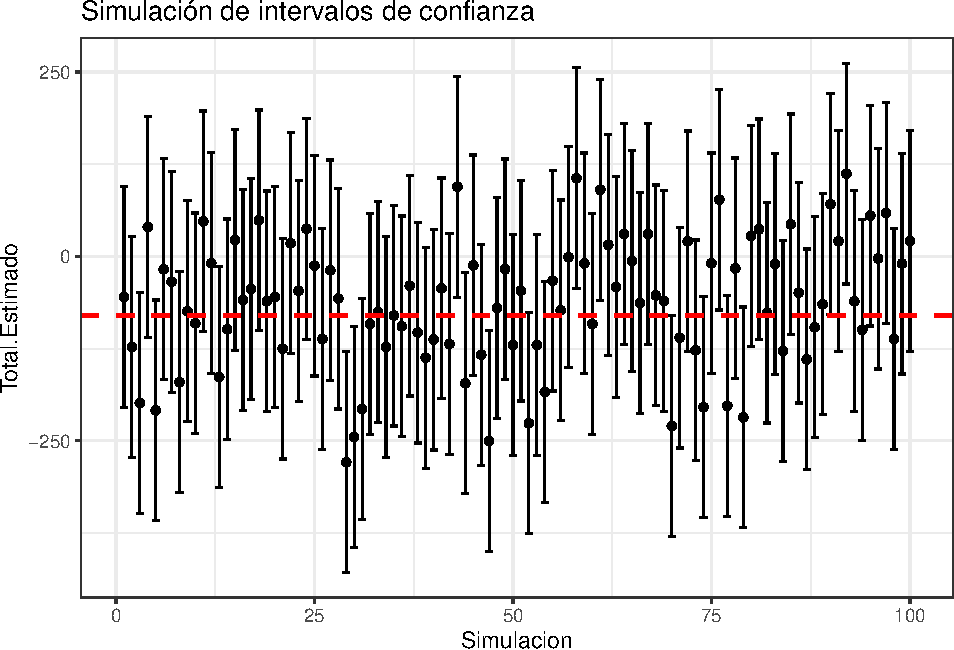
\includegraphics{Introduccion_a_Muestreo_files/figure-latex/unnamed-chunk-154-1.pdf}

Nota que estos intervalos son aproximados y no siempre van a funcionar. (¿Puedes hallar un ejemplo donde no sirvan a pesar de que \(n\) y \(N\) sean grandes?) Luego veremos correcciones a esto; por ahora, supondremos que la aproximación es buena.

\hypertarget{ejemplo-resumen-estimaciuxf3n-de-una-proporciuxf3n-bajo-muestreo-aleatorio-simple-sin-reemplazo}{%
\section{Ejemplo Resumen: Estimación de una proporción bajo muestreo aleatorio simple sin reemplazo}\label{ejemplo-resumen-estimaciuxf3n-de-una-proporciuxf3n-bajo-muestreo-aleatorio-simple-sin-reemplazo}}

Se realiza una encuesta mediante muestreo aleatorio simple sin reemplazo a la población del ITAM \(N = 5000\) donde interesa conocer la proporción de gente que apoya al gobierno en turno \(p\). Implícitamente, se supone que alguien apoya (proporción \(p\) de toda la población) o no lo apoya (proporción \(1-p\)), que dichos conjuntos son disjuntos y que no hay una tercera opción (como \texttt{NO\ RESPONDE\ /\ DESCONOCE\ QUIÉN\ GOBIERNA}). La pregunta es: ¿a cuántas personas hay que encuestar si interesa estimar \(p\) con un error máximo de tamaño \(\epsilon = 0.05\) al \(99\%\) de confianza (es decir, que el estimador \(\hat{p}\) de la proporción esté, a lo más, a \(\pm 0.05\) de distancia del valor verdadero \(p\) con un intervalo de confianza al \(99\%\))?

Supongamos tomamos una muestra de tamaño \(n\) dada por \(\mathcal{S} = (x_1, x_2, \dots, x_n)^T\) de una población \(\mathcal{U} = (x_1, x_2, \dots, x_N)^T\) de tamaño \(N\). Pensemos, además, existen \(N_1\) personas que aprueban al gobierno actual y \(N- N_1\) que desaprueban del mismo y por tanto la proporción que nos interesa estimar es:
\[
p = \dfrac{N_1}{N}
\]
Por otro lado, la proporción muestral de personas que aprueban está dada por:
\[
\hat{p} = \dfrac{\sum_{i = 1}^n \mathbb{I}_{\text{Aprueba}}(x_i)}{n}
\]
donde si definimos \(H = \dfrac{\sum_{i = 1}^n \mathbb{I}_{\text{Aprueba}}(x_i)}{n}\) notamos que la distribución de \(H\) está dada por una variable \href{https://en.wikipedia.org/wiki/Hypergeometric_distribution}{Hipergeométrica} (pues de una población de \(N\) se seleccionan \(n\) donde \(N_1\) cumplen la categoría deseada). Su media y varianza están dadas respectivamente por:
\[
\mathbb{E}\big[ H \big] = n \dfrac{N_1}{N} = np
\]
así como por:
\[
\textrm{Var}\big[ H\big] = n \dfrac{N_1}{N} \Big( 1 - \dfrac{N_1}{N}\Big) \Big( \dfrac{N-n}{N-1}\Big) = np (1-p)\Big( \dfrac{N-n}{N-1}\Big)
\]
Se sigue entonces que \(\mathbb{E}\big[\hat{p}\big] = p\) y por tanto \(\hat{p}\) es un estimador insesgado. La varianza por otro lado es:
\[
\textrm{Var}\big( \hat{p} \big) = \dfrac{p(1-p)}{n}\Big( \dfrac{N-n}{N-1}\Big)
\]
Finalmente, el estimador de la varianza es:
\[
\widehat{\textrm{Var}}\big( \hat{p} \big) = \dfrac{\hat{p}(1-\hat{p})}{n}\Big( \dfrac{N-n}{N-1}\Big)
\]
el cual también cumple que es insesgado (demuéstralo).

Podemos aplicar el Teorema Central del Límite para la proporción\footnote{Una mejor distribución sería una \(t\) de Student; empero eso lo verás en Estadística Matemática.} notando que la definición de \(\hat{p}\) coincide con una media (de las indicadoras):
\[
\underbrace{\dfrac{\hat{p} - p}{\sqrt{\frac{\hat{p}(1-\hat{p})}{n} \Big( \frac{N-n}{N-1} \Big)}}}_{\widehat{\text{Var}}(\hat{p})}\mathrel{\dot\sim} \textrm{Normal}(0,1)
\]
De donde se tiene que:
\begin{equation}
\begin{aligned}
& \mathbb{P}\Bigg(- z_{\alpha/2} \leq \dfrac{\hat{p} - p}{\sqrt{\frac{\hat{p}(1-\hat{p})}{n} \Big( \frac{N-n}{N-1} \Big)}}\leq z_{\alpha/2}\Bigg) \approx 1 - \alpha \\
\Rightarrow & \mathbb{P}\Bigg( \hat{p} - z_{\alpha/2} \sqrt{\frac{\hat{p}(1-\hat{p})}{n} \Big( \frac{N-n}{N-1} \Big)} \leq  p \leq \hat{p} +  z_{\alpha/2} \sqrt{\frac{\hat{p}(1-\hat{p})}{n} \Big( \frac{N-n}{N-1} \Big)}\Bigg) \approx 1 - \alpha 
\end{aligned}
\end{equation}

\begin{quote}
\textbf{Nota} \href{https://opentextbc.ca/introbusinessstatopenstax/chapter/a-confidence-interval-for-a-population-proportion/}{Es común encontrar en Internet} que para los intervalos de confianza la gente supone una población muy grande \(N\) respecto a la muestra \(n\) y entonces eliminan el término \(\frac{N-n}{N-1}\) argumentando que \(\frac{N-n}{N-1} \approx 1\) y obtienen la siguiente fórmula:
\[
\hat{p} \pm z_{\alpha/2} \sqrt{\frac{\hat{p}(1-\hat{p})}{n}} 
\]
esto simplifica algunos cálculos (a mano) pero nosotros tenemos \texttt{R} y podemos hacer cálculos más exactos sin tener que suponer semejantes atrocidades.
\end{quote}

Como el error deseado es de tamaño \(\epsilon\) queremos \(|p - \hat{p} | \leq \epsilon\) esto se traduce en:
\begin{equation}\nonumber
|p -  \hat{p}| \leq \underbrace{z_{\alpha/2} \sqrt{\frac{\hat{p}(1-\hat{p})}{n} \Big( \frac{N-n}{N-1} \Big) }}_{\epsilon}
\end{equation}
de donde igualamos para despejar la \(n\):
\begin{equation}\nonumber
\begin{aligned}
 \epsilon & = z_{\alpha/2} \sqrt{\frac{\hat{p}(1-\hat{p})}{n}\Big( \frac{N-n}{N-1} \Big)} \\
 & = \dfrac{\epsilon^2 }{z_{\alpha/2}^2} = \frac{\hat{p}(1-\hat{p})}{n}\Big( \frac{N-n}{N-1} \Big) \\
 & = \frac{N-1}{\hat{p}(1-\hat{p})}\dfrac{\epsilon^2 }{z_{\alpha/2}^2} =  \frac{N-n}{n} = \frac{N}{n} - 1 \\
 & = \frac{N-1}{\hat{p}(1-\hat{p})}\dfrac{\epsilon^2 }{z_{\alpha/2}^2} + 1 =  \frac{N}{n} \\
 & \Rightarrow n = \dfrac{N}{\frac{N-1}{\hat{p}(1-\hat{p})}\frac{\epsilon^2 }{z_{\alpha/2}^2} + 1} = \dfrac{\frac{z^2_{\alpha/2}}{\epsilon^2}\hat{p}(1-\hat{p})}{\frac{N-1}{N} + \frac{1}{N}\frac{z^2_{\alpha/2}}{\epsilon^2}\hat{p}(1-\hat{p})} = \dfrac{m}{1 + \frac{m-1}{N}}
\end{aligned}
\end{equation}
donde
\[
m = \frac{z^2_{\alpha/2}}{\epsilon^2}\hat{p}(1-\hat{p})
\]
Ahora el problema es que el tamaño de muestra \(n\) depende de la muestra a través de \(\hat{p}\) ¡y no hemos tomado la muestra! Para ello entonces analizamos el peor caso que puede ocurrir de \(\hat{p}\) de tal forma que obtengamos la \(n\) que puede salir con la peor proporción \(\hat{p}\) posible. Para ello maximizamos con derivadas:
\begin{equation}\nonumber
    \begin{aligned}
    \dfrac{\partial n}{\partial \hat{p}} & = \dfrac{\partial}{\partial \hat{p}} \Bigg(  \dfrac{N}{\frac{N-1}{\hat{p}(1-\hat{p})}\frac{\epsilon^2 }{z_{\alpha/2}^2} + 1} \Bigg) 
    \\ & = N  \Bigg(  \dfrac{1}{\frac{N-1}{\hat{p}(1-\hat{p})}\frac{\epsilon^2 }{z_{\alpha/2}^2} + 1} \Bigg)^2 \cdot \dfrac{\partial}{\partial \hat{p}} \Bigg( \frac{N-1}{\hat{p}(1-\hat{p})}\frac{\epsilon^2 }{z_{\alpha/2}^2} + 1\Bigg)  
    \\ & = \underbrace{N (N-1)\frac{\epsilon^2 }{z_{\alpha/2}^2}}_{C}  \Bigg(  \dfrac{1}{\frac{N-1}{\hat{p}(1-\hat{p})}\frac{\epsilon^2 }{z_{\alpha/2}^2} + 1} \Bigg)^2 \cdot \dfrac{\partial}{\partial \hat{p}} \Bigg( \frac{1}{\hat{p}(1-\hat{p})}\Bigg)  
    \\ & = C \Bigg(  \dfrac{1}{\frac{N-1}{\hat{p}(1-\hat{p})}\frac{\epsilon^2 }{z_{\alpha/2}^2} + 1} \Bigg)^2  \Bigg( \frac{1}{\hat{p}(1-\hat{p})}\Bigg)^2 \dfrac{\partial}{\partial \hat{p}} \hat{p}(1-\hat{p}) 
    \\ & = C \Bigg(  \dfrac{1}{\frac{N-1}{\hat{p}(1-\hat{p})}\frac{\epsilon^2 }{z_{\alpha/2}^2} + 1} \Bigg)^2  \Bigg( \frac{1}{\hat{p}(1-\hat{p})}\Bigg)^2  (1-2\hat{p}) = 0
    \end{aligned}
\end{equation}
de donde se sigue que \(\hat{p} = \frac{1}{2}\) es un punto crítico. De hecho puede verificarse que es el máximo (por ejemplo a través de la segunda derivada). Luego, podemos estimar la \(n\) de la muestra mediante:
\[
n = \left\lceil \dfrac{m}{1 + \frac{m-1}{N}} \right\rceil
\]
donde \(m = \dfrac{1}{4}\frac{z^2_{\alpha/2}}{\epsilon^2}\). En el caso particular de este ejercicio, \(N = 5000\), \(\epsilon = 0.05\), \(\alpha = 0.01\) y \(z^2_{\alpha/2} \approx\) \texttt{qnorm(0.9)}. Luego podemos calcular:

\begin{Shaded}
\begin{Highlighting}[]
\NormalTok{alpha   }\OtherTok{\textless{}{-}} \FloatTok{0.01}
\NormalTok{z       }\OtherTok{\textless{}{-}} \FunctionTok{qnorm}\NormalTok{(}\DecValTok{1} \SpecialCharTok{{-}}\NormalTok{ alpha}\SpecialCharTok{/}\DecValTok{2}\NormalTok{)}
\NormalTok{epsilon }\OtherTok{\textless{}{-}} \FloatTok{0.05}
\NormalTok{m       }\OtherTok{\textless{}{-}}\NormalTok{ (}\DecValTok{1}\SpecialCharTok{/}\DecValTok{4}\NormalTok{)}\SpecialCharTok{*}\NormalTok{(z}\SpecialCharTok{/}\NormalTok{epsilon)}\SpecialCharTok{\^{}}\DecValTok{2}
\NormalTok{N       }\OtherTok{\textless{}{-}} \DecValTok{5000}
\NormalTok{n       }\OtherTok{\textless{}{-}} \FunctionTok{ceiling}\NormalTok{(m}\SpecialCharTok{/}\NormalTok{(}\DecValTok{1} \SpecialCharTok{+}\NormalTok{ (m}\DecValTok{{-}1}\NormalTok{)}\SpecialCharTok{/}\NormalTok{N))}

\FunctionTok{print}\NormalTok{(}\FunctionTok{paste0}\NormalTok{(}\StringTok{"El tamaño de muestra es "}\NormalTok{, n))}
\end{Highlighting}
\end{Shaded}

\begin{verbatim}
## [1] "El tamaño de muestra es 586"
\end{verbatim}

\hypertarget{ejemplo-resumen-estimaciuxf3n-del-total-de-individuos-en-una-fotografuxeda}{%
\section{Ejemplo Resumen: Estimación del total de individuos en una fotografía}\label{ejemplo-resumen-estimaciuxf3n-del-total-de-individuos-en-una-fotografuxeda}}

En este ejercicio vamos a determinar cuánta gente aparece en la siguiente foto:

\begin{figure}

{\centering 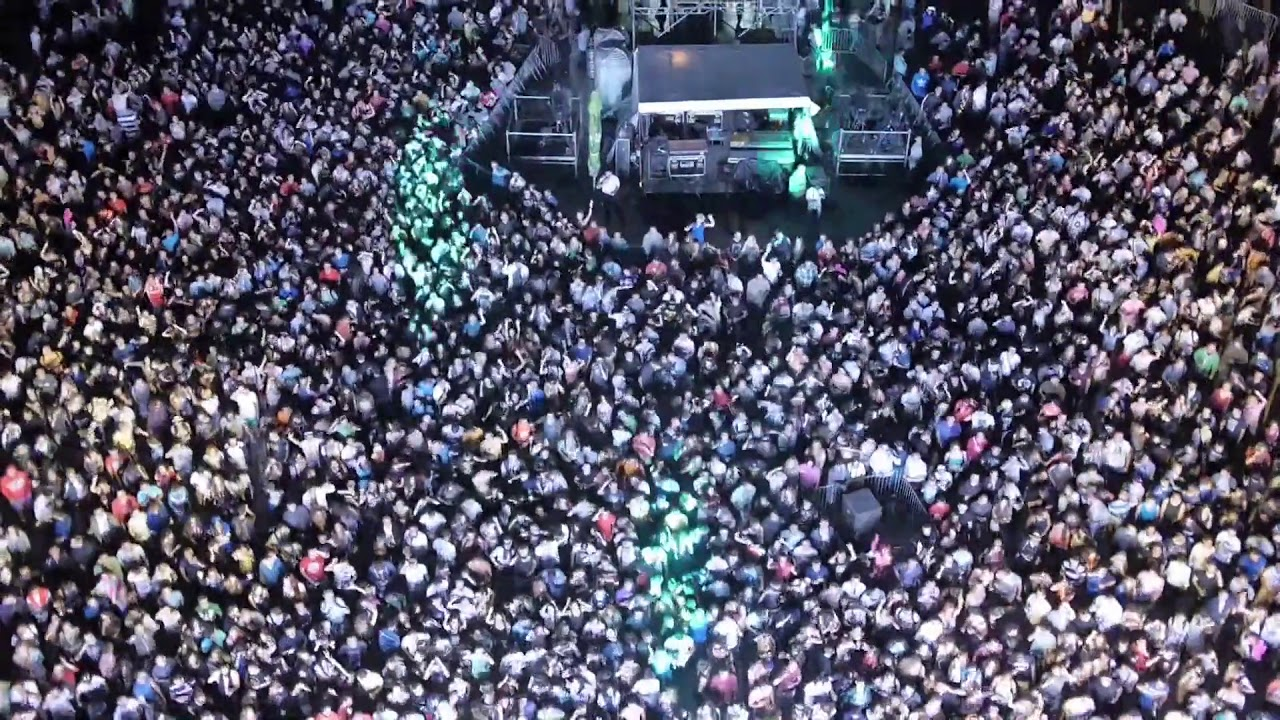
\includegraphics[width=0.75\linewidth]{images/concierto} 

}

\caption{Imagen de un concierto extraída de https://www.youtube.com/watch?v=pJ1YKwyH5bk}\label{fig:unnamed-chunk-156}
\end{figure}

Hay varias opciones para determinar la cantidad de gente que está en dicha foto. Una sería contar todas las cabecitas que aparecen; otra, diseñar un modelo de redes neuronales (o de \href{https://yangliang.github.io/pdf/sp055u.pdf}{convolusión} porque a la gente le encanta eso) que identifique una cabeza y la cuente. Nosotros lo que haremos (por ser un curso de estadística) será muestrear. Como investigador me interesa responder la siguiente pregunta:

\begin{quote}
¿Cuánta gente está en la fotografía con un intervalo de error de \(\pm 50\) casos al 95\%?
\end{quote}

Para ello dividiremos la fotografía en \(N\) pedazos (a determinar), muestrearemos \(n\) de ellos y contaremos la cantidad de personas que aparecen en cada pedazo. Finalmente, generamos intervalos de confianza y de muestreo. Para ello repetimos el ejercicio anterior de despejar la \(n\) del intervalo de confianza; por el teorema del límite central tenemos:

\[
\dfrac{\hat{t} - t}{\sqrt{\textrm{Var}(\hat{t})}} ~\sim \textrm{Normal}(0,1)
\]
de donde obtenemos intervalos (¡verifícalo!) de la forma:
\[
 \hat{t} \pm z_{1-\alpha/2}\cdot\sqrt{\textrm{Var}(\hat{t})} 
\]
Donde podemos aproximar la varianza mediante \(\widehat{\text{Var}}(\hat{t}) = N^2\dfrac{1-f}{n} s^2_{x,\mathcal{S}}\) donde recordamos que \(f = n/N\) y \(s^2_{x,\mathcal{S}}\) es la varianza muestral. Tomamos \(\epsilon = 50\) y despejamos:

\begin{equation}\nonumber
\begin{aligned}
 \epsilon & =  z_{1-\alpha/2}\cdot\sqrt{\textrm{Var}(\hat{t})} \\
 \Rightarrow \dfrac{\epsilon^2}{z_{1-\alpha/2}^2} & = N^2\dfrac{1-f}{n} s^2_{x,\mathcal{S}}   \\
 \Rightarrow \dfrac{\epsilon^2}{z_{1-\alpha/2}^2 s^2_{x,\mathcal{S}} N^2} & = \dfrac{1-\frac{n}{N}}{n} \\
 \Rightarrow \dfrac{\epsilon^2}{z_{1-\alpha/2}^2 s^2_{x,\mathcal{S}} N^2} & = \dfrac{1}{n} - \dfrac{1}{N} \\
 \Rightarrow \dfrac{\epsilon^2}{z_{1-\alpha/2}^2 s^2_{x,\mathcal{S}} N^2} + \dfrac{1}{N} & = \dfrac{1}{n}  \\
 \Rightarrow \dfrac{1}{N} \Bigg( \dfrac{\epsilon^2}{z_{1-\alpha/2}^2 s^2_{x,\mathcal{S}} N} + 1 \Bigg) & = \dfrac{1}{n}  \\
  \Rightarrow \dfrac{1}{N} \Bigg( \dfrac{\epsilon^2 + z_{1-\alpha/2}^2 s^2_{x,\mathcal{S}} N}{z_{1-\alpha/2}^2 s^2_{x,\mathcal{S}} N} \Bigg) & = \dfrac{1}{n}  \\
  \Rightarrow  \Bigg( \dfrac{(z_{1-\alpha/2} s_{x,\mathcal{S}} N)^2} {\epsilon^2 + z_{1-\alpha/2}^2 s^2_{x,\mathcal{S}} N}\Bigg) & = n  \\
\end{aligned}
\end{equation}

El problema aquí es que la \(n\) depende de la varianza muestral \(s^2_{x,\mathcal{S}}\) (actualmente desconocida) así como de la cantidad de cuadritos originales \(N\) en los que dividimos la foto. Hay en la literatura varias técnicas que se pueden utilizar para estimar el \(s^2_{x,\mathcal{S}}\):

\begin{enumerate}
\def\labelenumi{\arabic{enumi}.}
\item
  Realizar un estudio piloto (es decir un pequeño ejemplo de lo que vas a hacer en una población chica y de ahí tener la varianza). Esta es la mejor opción.
\item
  Buscar otros estudios similares donde se analicen objetos similares de estudio y ver sus varianzas; suponer que la de este estudio es similar. Esta es la segunda mejor opción.
\item
  Inventártela (sí, es una opción pero no la mejor). Vamos, ¿cuál es la probabilidad de que nadie en todo el mundo haya hecho un análisis similar al tuyo? Si realmente estás haciendo algo completamente nuevo \emph{sin estudio piloto} pues\ldots{} podrías inventarla. ¿Lo recomiendo? No; pero pasa.
\end{enumerate}

En nuestro caso utilizaremos la varianza estimada \href{https://arxiv.org/pdf/1903.07427.pdf}{de este artículo} reportada en \(1.02\); luego \(s^2_{x,\mathcal{S}} \approx 1.02\) para nuestro análisis.

Finalmente, como éste es sólo un ejercicio de clase tomaremos \(N = 100\) (dividir la foto en \(100\) cuadritos). De manera profesional, de nuevo habría que ver diferencias en los resultados de las estimaciones en función de los cuadritos, o bien asignar un costo a la cantidad de cuadros. Concluimos entonces que para nuestro estudio:

\[
n = \left\lceil \dfrac{(z_{1-\alpha/2} s_{x,\mathcal{S}} N)^2} {\epsilon^2 + z_{1-\alpha/2}^2 s^2_{x,\mathcal{S}} N}\right\rceil  = \left\lceil \dfrac{(1.95\cdot \sqrt{1.02} \cdot 100)^2} {50^2 + 1.95^2\cdot 1.02 \cdot 100}\right\rceil
\]
Podemos calcular en \texttt{R}:

\begin{Shaded}
\begin{Highlighting}[]
\NormalTok{n }\OtherTok{\textless{}{-}} \FunctionTok{ceiling}\NormalTok{((}\FunctionTok{qnorm}\NormalTok{(}\FloatTok{0.975}\NormalTok{)}\SpecialCharTok{*}\FunctionTok{sqrt}\NormalTok{(}\FloatTok{1.02}\NormalTok{)}\SpecialCharTok{*}\DecValTok{100}\NormalTok{)}\SpecialCharTok{\^{}}\DecValTok{2}\SpecialCharTok{/}\NormalTok{(}\DecValTok{50}\SpecialCharTok{\^{}}\DecValTok{2} \SpecialCharTok{+}\NormalTok{ (}\FunctionTok{qnorm}\NormalTok{(}\FloatTok{0.975}\NormalTok{)}\SpecialCharTok{\^{}}\DecValTok{2}\SpecialCharTok{*}\FloatTok{1.02}\SpecialCharTok{*}\DecValTok{100}\NormalTok{)))}
\FunctionTok{print}\NormalTok{(}\FunctionTok{paste0}\NormalTok{(}\StringTok{"El tamaño de muestra es "}\NormalTok{, n))}
\end{Highlighting}
\end{Shaded}

\begin{verbatim}
## [1] "El tamaño de muestra es 14"
\end{verbatim}

Podemos proceder a dividir la foto en los \(N = 100\) pedazos:

\begin{Shaded}
\begin{Highlighting}[]
\CommentTok{\#División con base en el siguiente link:}
\CommentTok{\#https://rpubs.com/issactoast/cutimage}
\FunctionTok{library}\NormalTok{(imager)}

\CommentTok{\#Cargamos la imagen}
\NormalTok{img }\OtherTok{\textless{}{-}} \FunctionTok{load.image}\NormalTok{(}\StringTok{"images/concierto.jpg"}\NormalTok{)}

\CommentTok{\#Función auxiliar del link superior}
\NormalTok{make.vr }\OtherTok{\textless{}{-}} \ControlFlowTok{function}\NormalTok{( x, name )\{}
  \FunctionTok{assign}\NormalTok{( name, x, }\AttributeTok{envir =}\NormalTok{ .GlobalEnv)}
\NormalTok{\}}

\CommentTok{\#División en N}
\NormalTok{N }\OtherTok{\textless{}{-}} \DecValTok{100}
\FunctionTok{par}\NormalTok{(}\AttributeTok{mfrow=}\FunctionTok{c}\NormalTok{(}\FunctionTok{sqrt}\NormalTok{(N),}\FunctionTok{sqrt}\NormalTok{(N)), }\AttributeTok{mar =} \FunctionTok{c}\NormalTok{(}\FloatTok{0.1}\NormalTok{,}\FloatTok{0.1}\NormalTok{,}\FloatTok{0.1}\NormalTok{,}\FloatTok{0.1}\NormalTok{))}
\NormalTok{k }\OtherTok{\textless{}{-}} \DecValTok{1}
\ControlFlowTok{for}\NormalTok{ (j }\ControlFlowTok{in} \DecValTok{1}\SpecialCharTok{:}\FunctionTok{sqrt}\NormalTok{(N))\{}
  \ControlFlowTok{for}\NormalTok{ (i }\ControlFlowTok{in} \DecValTok{1}\SpecialCharTok{:}\FunctionTok{sqrt}\NormalTok{(N))\{}
\NormalTok{    vr.name }\OtherTok{\textless{}{-}} \FunctionTok{paste0}\NormalTok{(}\StringTok{"sub"}\NormalTok{, k)}
\NormalTok{    k       }\OtherTok{\textless{}{-}}\NormalTok{ k }\SpecialCharTok{+} \DecValTok{1}
    \FunctionTok{imsub}\NormalTok{(img, (width}\SpecialCharTok{/}\FunctionTok{sqrt}\NormalTok{(N))}\SpecialCharTok{*}\NormalTok{(i}\DecValTok{{-}1}\NormalTok{) }\SpecialCharTok{\textless{}}\NormalTok{ x }\SpecialCharTok{\&}\NormalTok{ x }\SpecialCharTok{\textless{}}\NormalTok{  i }\SpecialCharTok{*}\NormalTok{ (width}\SpecialCharTok{/}\FunctionTok{sqrt}\NormalTok{(N)),}
\NormalTok{          (height}\SpecialCharTok{/}\FunctionTok{sqrt}\NormalTok{(N))}\SpecialCharTok{*}\NormalTok{(j}\DecValTok{{-}1}\NormalTok{) }\SpecialCharTok{\textless{}}\NormalTok{ y }\SpecialCharTok{\&}\NormalTok{ y }\SpecialCharTok{\textless{}}\NormalTok{  j }\SpecialCharTok{*}\NormalTok{ (height}\SpecialCharTok{/}\FunctionTok{sqrt}\NormalTok{(N))) }\SpecialCharTok{\%\textgreater{}\%}
      \FunctionTok{make.vr}\NormalTok{(}\AttributeTok{name =}\NormalTok{ vr.name) }\SpecialCharTok{\%\textgreater{}\%}
      \CommentTok{\# save.image( file = paste0(vr.name,".jpg")) \%\textgreater{}\%}
      \FunctionTok{plot}\NormalTok{(}\AttributeTok{axes =} \ConstantTok{FALSE}\NormalTok{,}
           \AttributeTok{xaxt=}\StringTok{"n"}\NormalTok{, }\AttributeTok{yaxt=}\StringTok{"n"}\NormalTok{, }
           \AttributeTok{xlab =} \StringTok{""}\NormalTok{, }\AttributeTok{ylab =} \StringTok{""}\NormalTok{, }\AttributeTok{ann =} \ConstantTok{FALSE}\NormalTok{ )    }
\NormalTok{  \}}
\NormalTok{\}}
\end{Highlighting}
\end{Shaded}

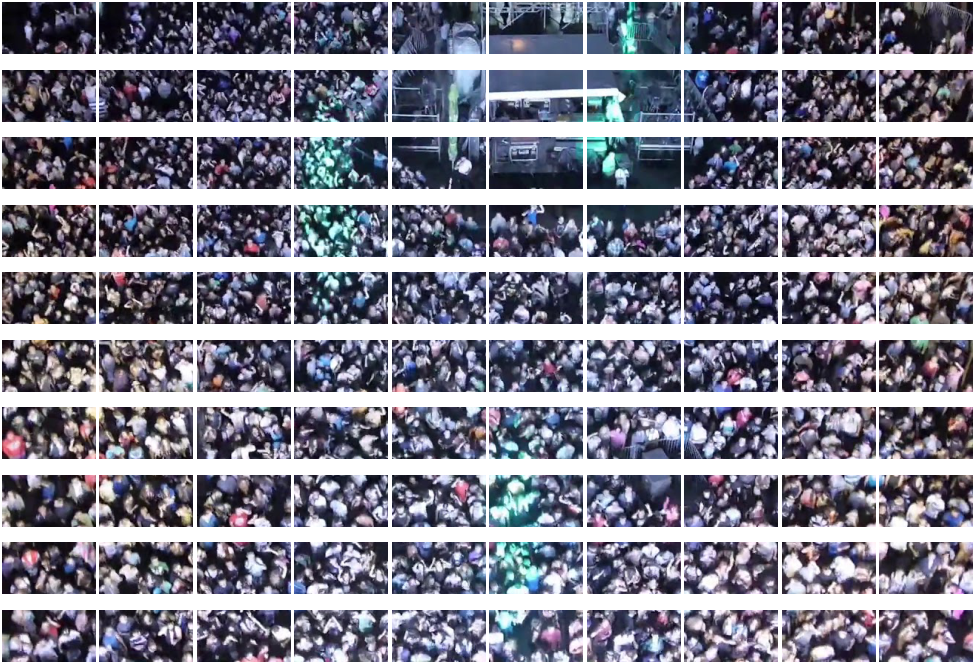
\includegraphics{Introduccion_a_Muestreo_files/figure-latex/unnamed-chunk-158-1.pdf}

Podemos acceder a cada una de las imágenes que se tienen a través de su nombre (\texttt{sub} seguido de un número entre \(0\) y \(100\)). Muestreamos entonces los nombres de las 15 imágenes:

\begin{Shaded}
\begin{Highlighting}[]
\CommentTok{\#Obtenemos los dígitos a muestrear}
\NormalTok{imagenes.muestreadas }\OtherTok{\textless{}{-}} \FunctionTok{sample}\NormalTok{(}\DecValTok{1}\SpecialCharTok{:}\DecValTok{100}\NormalTok{, n, }\AttributeTok{replace =} \ConstantTok{FALSE}\NormalTok{)}

\CommentTok{\#Agregamos el prefijo sub}
\NormalTok{imagenes.muestreadas }\OtherTok{\textless{}{-}} \FunctionTok{paste0}\NormalTok{(}\StringTok{"sub"}\NormalTok{, imagenes.muestreadas)}
\end{Highlighting}
\end{Shaded}

Y graficamos cada una de ellas:

\begin{Shaded}
\begin{Highlighting}[]
\FunctionTok{par}\NormalTok{(}\AttributeTok{mfrow =} \FunctionTok{c}\NormalTok{(}\DecValTok{1}\NormalTok{,}\DecValTok{1}\NormalTok{))}

\ControlFlowTok{for}\NormalTok{ (imagen }\ControlFlowTok{in}\NormalTok{ imagenes.muestreadas)\{}
  \FunctionTok{plot}\NormalTok{(}\FunctionTok{get}\NormalTok{(imagen),  }\AttributeTok{main =}\NormalTok{ imagen, }\AttributeTok{axes =} \ConstantTok{FALSE}\NormalTok{)}
\NormalTok{\}}
\end{Highlighting}
\end{Shaded}

\begin{center}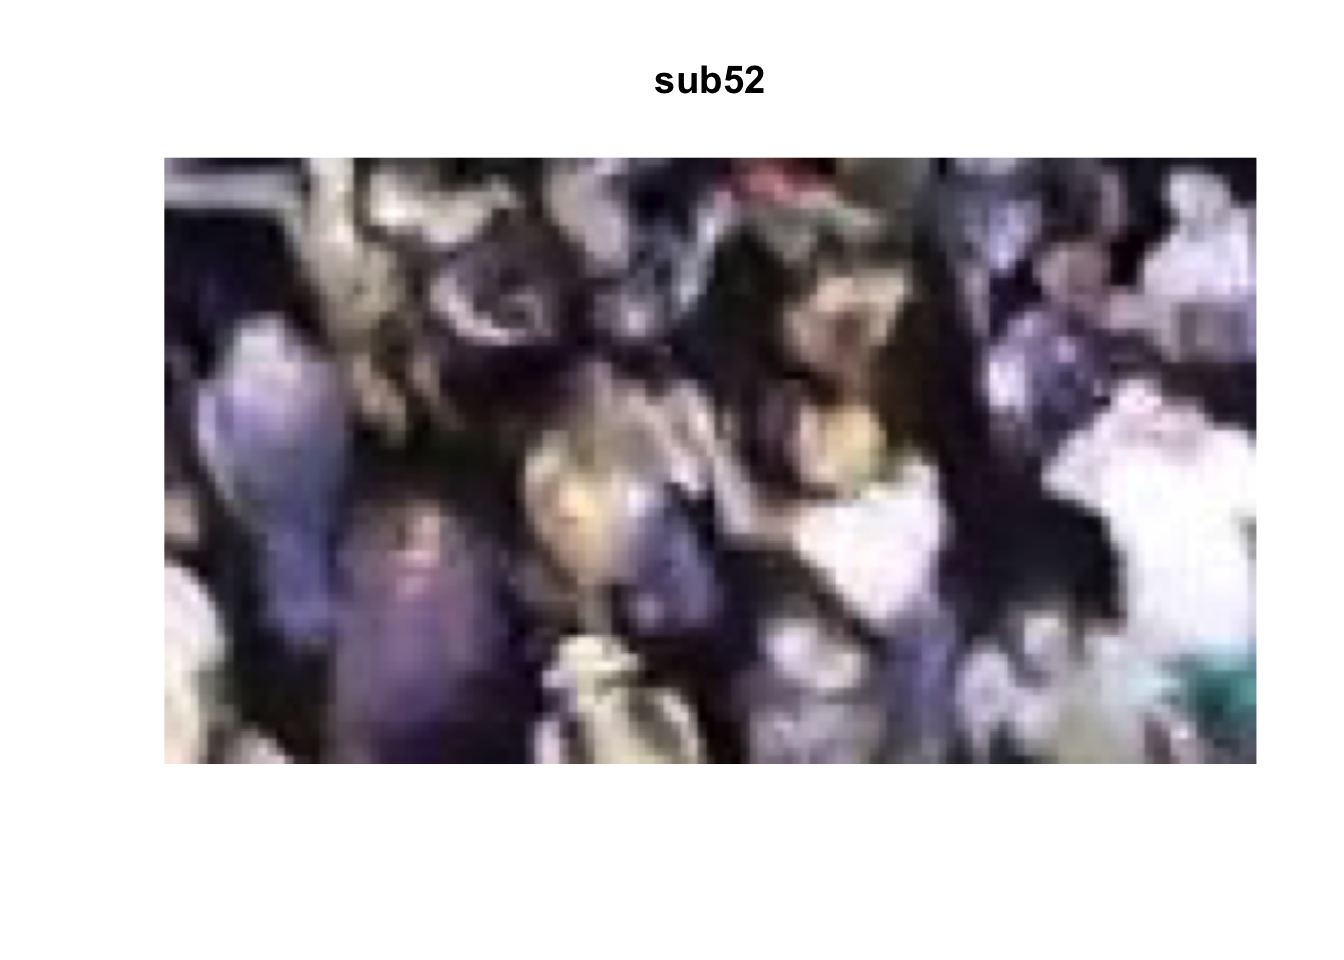
\includegraphics[width=0.5\linewidth]{Introduccion_a_Muestreo_files/figure-latex/unnamed-chunk-160-1} \end{center}

\begin{center}\includegraphics[width=0.5\linewidth]{Introduccion_a_Muestreo_files/figure-latex/unnamed-chunk-160-2} \end{center}

\begin{center}\includegraphics[width=0.5\linewidth]{Introduccion_a_Muestreo_files/figure-latex/unnamed-chunk-160-3} \end{center}

\begin{center}\includegraphics[width=0.5\linewidth]{Introduccion_a_Muestreo_files/figure-latex/unnamed-chunk-160-4} \end{center}

\begin{center}\includegraphics[width=0.5\linewidth]{Introduccion_a_Muestreo_files/figure-latex/unnamed-chunk-160-5} \end{center}

\begin{center}\includegraphics[width=0.5\linewidth]{Introduccion_a_Muestreo_files/figure-latex/unnamed-chunk-160-6} \end{center}

\begin{center}\includegraphics[width=0.5\linewidth]{Introduccion_a_Muestreo_files/figure-latex/unnamed-chunk-160-7} \end{center}

\begin{center}\includegraphics[width=0.5\linewidth]{Introduccion_a_Muestreo_files/figure-latex/unnamed-chunk-160-8} \end{center}

\begin{center}\includegraphics[width=0.5\linewidth]{Introduccion_a_Muestreo_files/figure-latex/unnamed-chunk-160-9} \end{center}

\begin{center}\includegraphics[width=0.5\linewidth]{Introduccion_a_Muestreo_files/figure-latex/unnamed-chunk-160-10} \end{center}

\begin{center}\includegraphics[width=0.5\linewidth]{Introduccion_a_Muestreo_files/figure-latex/unnamed-chunk-160-11} \end{center}

\begin{center}\includegraphics[width=0.5\linewidth]{Introduccion_a_Muestreo_files/figure-latex/unnamed-chunk-160-12} \end{center}

\begin{center}\includegraphics[width=0.5\linewidth]{Introduccion_a_Muestreo_files/figure-latex/unnamed-chunk-160-13} \end{center}

\begin{center}\includegraphics[width=0.5\linewidth]{Introduccion_a_Muestreo_files/figure-latex/unnamed-chunk-160-14} \end{center}

Para cada una de las imágenes contamos las cabecitas que aparecen:

\begin{Shaded}
\begin{Highlighting}[]
\NormalTok{datos }\OtherTok{\textless{}{-}} \FunctionTok{data.frame}\NormalTok{(}
  \AttributeTok{Imagen =}\NormalTok{ imagenes.muestreadas,}
  \AttributeTok{Conteo =} \FunctionTok{c}\NormalTok{(}\DecValTok{13}\NormalTok{, }\DecValTok{11}\NormalTok{, }\DecValTok{9}\NormalTok{, }\DecValTok{14}\NormalTok{, }\DecValTok{9}\NormalTok{, }\DecValTok{15}\NormalTok{, }\DecValTok{14}\NormalTok{, }\DecValTok{10}\NormalTok{, }\DecValTok{1}\NormalTok{, }\DecValTok{22}\NormalTok{, }\DecValTok{8}\NormalTok{, }\DecValTok{9}\NormalTok{, }\DecValTok{17}\NormalTok{, }\DecValTok{16}\NormalTok{)}
\NormalTok{)}
\FunctionTok{kable}\NormalTok{(datos) }\SpecialCharTok{\%\textgreater{}\%} \FunctionTok{kable\_styling}\NormalTok{(}\AttributeTok{latex\_options =} \StringTok{"striped"}\NormalTok{)}
\end{Highlighting}
\end{Shaded}

\begin{table}
\centering
\begin{tabular}{l|r}
\hline
Imagen & Conteo\\
\hline
\cellcolor{gray!6}{sub52} & \cellcolor{gray!6}{13}\\
\hline
sub43 & 11\\
\hline
\cellcolor{gray!6}{sub34} & \cellcolor{gray!6}{9}\\
\hline
sub35 & 14\\
\hline
\cellcolor{gray!6}{sub54} & \cellcolor{gray!6}{9}\\
\hline
sub23 & 15\\
\hline
\cellcolor{gray!6}{sub83} & \cellcolor{gray!6}{14}\\
\hline
sub14 & 10\\
\hline
\cellcolor{gray!6}{sub79} & \cellcolor{gray!6}{1}\\
\hline
sub5 & 22\\
\hline
\cellcolor{gray!6}{sub30} & \cellcolor{gray!6}{8}\\
\hline
sub36 & 9\\
\hline
\cellcolor{gray!6}{sub39} & \cellcolor{gray!6}{17}\\
\hline
sub16 & 16\\
\hline
\end{tabular}
\end{table}

Tenemos entonces que la estimación del total \(\hat{t}\) es: 1200, por otro lado la varianza muestral es \(s_{x,\mathcal{S}}\) está dada por: 25.2307692. Podemos entonces establecer un intervalo de confianza para el total:

\begin{Shaded}
\begin{Highlighting}[]
\NormalTok{x  }\OtherTok{\textless{}{-}} \FunctionTok{c}\NormalTok{(}\DecValTok{13}\NormalTok{, }\DecValTok{11}\NormalTok{, }\DecValTok{9}\NormalTok{, }\DecValTok{14}\NormalTok{, }\DecValTok{9}\NormalTok{, }\DecValTok{15}\NormalTok{, }\DecValTok{14}\NormalTok{, }\DecValTok{10}\NormalTok{, }\DecValTok{1}\NormalTok{, }\DecValTok{22}\NormalTok{, }\DecValTok{8}\NormalTok{, }\DecValTok{9}\NormalTok{, }\DecValTok{17}\NormalTok{, }\DecValTok{16}\NormalTok{, }\DecValTok{10}\NormalTok{)}
\NormalTok{s2            }\OtherTok{\textless{}{-}} \FunctionTok{var}\NormalTok{(x)}
\NormalTok{N             }\OtherTok{\textless{}{-}} \DecValTok{100}
\NormalTok{n             }\OtherTok{\textless{}{-}} \DecValTok{15}
\NormalTok{total.muestra }\OtherTok{\textless{}{-}}\NormalTok{ N}\SpecialCharTok{*}\FunctionTok{mean}\NormalTok{(x)}
\NormalTok{ci            }\OtherTok{\textless{}{-}} \FunctionTok{qnorm}\NormalTok{(}\FloatTok{0.975}\NormalTok{)}\SpecialCharTok{*}\FunctionTok{sqrt}\NormalTok{(N}\SpecialCharTok{\^{}}\DecValTok{2}\SpecialCharTok{*}\NormalTok{(}\DecValTok{1} \SpecialCharTok{{-}}\NormalTok{ n}\SpecialCharTok{/}\NormalTok{N)}\SpecialCharTok{/}\NormalTok{n}\SpecialCharTok{*}\NormalTok{s2)}
\NormalTok{ci\_low        }\OtherTok{\textless{}{-}} \FunctionTok{round}\NormalTok{(total.muestra }\SpecialCharTok{{-}}\NormalTok{ ci,}\DecValTok{2}\NormalTok{)}
\NormalTok{ci\_up         }\OtherTok{\textless{}{-}} \FunctionTok{round}\NormalTok{(total.muestra }\SpecialCharTok{+}\NormalTok{ ci,}\DecValTok{2}\NormalTok{)}

\FunctionTok{print}\NormalTok{(}\FunctionTok{paste0}\NormalTok{(}\StringTok{"Se estiman "}\NormalTok{, }\FunctionTok{round}\NormalTok{(total.muestra,}\DecValTok{2}\NormalTok{), }\StringTok{" personas con intervalo de "}\NormalTok{,}
             \StringTok{"confianza al 95\% de ["}\NormalTok{, ci\_low, }\StringTok{" ,"}\NormalTok{, ci\_up,}\StringTok{"]"}\NormalTok{))}
\end{Highlighting}
\end{Shaded}

\begin{verbatim}
## [1] "Se estiman 1186.67 personas con intervalo de confianza al 95% de [959.55 ,1413.78]"
\end{verbatim}

\hypertarget{ejercicio-7}{%
\section{Ejercicio:}\label{ejercicio-7}}

Cuando se resgistra un paquete de \texttt{R} en \href{https://cran.r-project.org}{CRAN} estos se registran junto con sus autores como muestra la imagen:

\includegraphics[width=0.75\linewidth]{images/CRAN}

La información de un paquete puede encontrarse en la página de \texttt{CRAN} dando clic en \texttt{Packages} y luego en \texttt{Table\ of\ available\ packages,\ sorted\ by\ name} y buscando el paquete deseado.

Se desea conocer el número promedio de autores por paquete registrado en \texttt{CRAN} con un intervalo de confianza al 80\% y un error de \(\pm 1\). Obtén la \(n\) necesaria para muestrear, calcula un estimador de la media y obtén intervalos de confianza. Justifica tu elección de la varianza para la \(n\) mediante un estudio piloto (muestreando de manera inicial \(10\) y calculando la varianza de ellos).

\textbf{Hint} Para obtener una lista (censo) de todos los paquetes de \texttt{R} puedes utilizar la función \texttt{available.packages()} la cual devuelve una matriz con todos los paquetes e incluye la \texttt{url} de donde se encuentra.

\hypertarget{ejemplo-resumen-estimaciuxf3n-de-una-regiuxf3n-cruxedtica}{%
\section{Ejemplo Resumen: Estimación de una región crítica}\label{ejemplo-resumen-estimaciuxf3n-de-una-regiuxf3n-cruxedtica}}

En una elección existen dos candidatas \(A\) y \(B\). Se realiza una encuesta de opinión mediante muestreo aleatorio simple sin reemplazo donde se les pregunta a una cantidad suficiente de votantes por quién votarían de las dos. En este análisis no hay \texttt{NO\ SABE\ /\ NO\ RESPONDE} sino que todos los individuos indican su preferencia. Se desea determinar la cantidad de puntos porcentuales que debe haber de diferencia entre la proporción de individuos que reportan apoyan al candidato \(A\) y los que reportan que apoyan al \(B\) de tal forma que el \(95\%\) de las veces podamos declarar de manera adecuada al ganador.

\begin{quote}
\textbf{Nota} Si \(A\) no es el ganador entonces \(p_A < 50\%\) (la proporción de votantes que van a elegir a \(A\) es menor a la mitad) ¿cierto?
\end{quote}

Para ello el análisis es como sigue: sea \(\hat{p}_A\) un estimador de la proporción de individuos que van a elegir a \(A\) y \(p_A\) la verdadera proporción. Sin pérdida de generalidad supondremos que \(B\) es el ganador; es decir que \(p_A < 0.5\).
El problema puede traducirse en determinar una \(c\) tal que:
\[
\mathbb{P}\big( \hat{p}_A > c | p_A < 0.5 \big) \leq 0.05
\]
Notamos que el evento \(\{ p_A < 50\%\}\) es por definición conocido (con probabilidad \(0\) ó \(1\)) pues está dado por la población (constante). Notamos que por el teorema del límite central podemos escribir:
\[
\dfrac{\hat{p}_A - p_A}{\sqrt{\text{Var}(\hat{p}_A )}}\sim \text{Normal}\big(0, 1\big)
\]
donde \(\hat{p}_A = \frac{1}{N} \sum_{i = 1}^N x_i \mathbb{I}_{\mathcal{S}}(x_i)\) como anteriormente hicimos para proporciones y su varianza está dada por:
\[
\text{Var}(\hat{p}_A ) = \frac{p_A(1-p_A)}{n}\Big( \frac{N-1}{N-n}\Big)
\]
donde el cálculo se hizo en el primer ejemplo de esta sección. Podemos transformar el problema entonces en hallar \(c\) tal que:
\[
\mathbb{P}\bigg( \underbrace{\frac{\hat{p}_A - p_A}{\sqrt{\text{Var}(\hat{p}_A )}}}_{Z \sim \text{Normal}(0,1)} > \frac{c - p_A}{\sqrt{\text{Var}(\hat{p}_A)}} \bigg| p_A < 0.5 \bigg) \leq 0.05
\]
Notamos que el lado izquierdo tiene una aproximación normal y entonces podemos reescribir el problema como hallar \(c\) tal que:
\[
\mathbb{P}\bigg( Z > \frac{c - p_A}{\sqrt{\text{Var}(\hat{p}_A)}} \bigg| p_A < 0.5 \bigg) \leq 0.05 \qquad \text{ donde } Z \sim \text{Normal}(0,1).
\]

Recordando la expresión para la varianza sustituyo:
\[
\mathbb{P}\left( Z > \dfrac{c - p_A}{\sqrt{\frac{p_A(1-p_A)}{n}\Big( \frac{N-1}{N-n}\Big)}} \Bigg| p_A < 0.5 \right) \leq 0.05 \qquad \text{ donde } Z \sim \text{Normal}(0,1).
\]
En función del análisis pasado, observamos que \(\dfrac{c - p_A}{\sqrt{\frac{p_A(1-p_A)}{n}\Big( \frac{N-1}{N-n}\Big)}}\) es una función decreciente en términos de \(p_A\) (¡compruébalo!) y que el mínimo valor se alcanza en el máximo de la \(p_A\) en el intervalo; es decir cuando \(p_A = \frac{1}{2}\). Luego el problema se transforma en hallar \(c\) tal que:

\[
\mathbb{P}\left( Z > \dfrac{c - \frac{1}{2}}{\sqrt{\frac{\frac{1}{2}(1-\frac{1}{2})}{n}\Big( \frac{N-1}{N-n}\Big)}} \right) \leq 0.05 \qquad \text{ donde } Z \sim \text{Normal}(0,1).
\]
donde eliminamos el evento \(p_A < 0.5\) por ser un evento seguro. Reescribimos el evento:
\[
\underbrace{\mathbb{P}\left( Z < \dfrac{c - \frac{1}{2}}{\sqrt{\frac{\frac{1}{2}(1-\frac{1}{2})}{n}\Big( \frac{N-1}{N-n}\Big)}} \right)}_{\Phi(x)} \geq 0.95 \qquad \text{ donde } x = \dfrac{c - \frac{1}{2}}{\sqrt{\frac{\frac{1}{2}(1-\frac{1}{2})}{n}\Big( \frac{N-1}{N-n}\Big)}}
\]
de tal forma que descubrimos la acumulada de la normal; terminamos de escribir todo:
\[
\Phi(x) \geq 0.95
\]
donde aplicamos la función inversa de la acumulada de la normal para descubrir:
\[
\dfrac{c - \frac{1}{2}}{\sqrt{\frac{\frac{1}{2}(1-\frac{1}{2})}{n}\Big( \frac{N-1}{N-n}\Big)}} \geq \phi^{-1}(0.95) \Rightarrow c = \frac{1}{2} + \phi^{-1}(0.95)\sqrt{\frac{\frac{1}{2}(1-\frac{1}{2})}{n}\Big( \frac{N-1}{N-n}\Big)}
\]
de donde se sigue que:
\[
\hat{p}_{A} > \frac{1}{2}\Bigg(1 + \phi^{-1}(0.95)\sqrt{\frac{N-1}{n(N-n)}} \Bigg) \Rightarrow 2\hat{p}_A = 1 + \phi^{-1}(0.95)\sqrt{\frac{N-1}{n(N-n)}} 
\]
Notando que los puntos porcentuales de \(B\) estimados mediante \(\hat{p}_B\) tienen la forma:
\[
\hat{p}_B = 1 - \hat{p}_A
\]
se tiene entonces que la diferencia entre puntos para determinar quien gana es:
\[
\hat{p}_A - \hat{p}_B = 2\hat{p}_A - 1 \geq \phi^{-1}(0.95)\sqrt{\frac{N-1}{n(N-n)}} 
\]
El mismo análisis se seguiría bajo la hipótesis de que el perdedor es \(B\); por tanto se tiene que cumplir que:
\[
| \hat{p}_A - \hat{p}_B | \geq \phi^{-1}(0.95)\sqrt{\frac{N-1}{n(N-n)}} 
\]
para poder declarar como ganador a aquél con más puntos porcentuales de manera correcta con una confianza del \(95\%\).

\hypertarget{ejemplo-resumen-estimaciuxf3n-del-total-de-una-poblaciuxf3n}{%
\section{Ejemplo Resumen: Estimación del total de una población}\label{ejemplo-resumen-estimaciuxf3n-del-total-de-una-poblaciuxf3n}}

Consideremos una población de tiburones donde se desconoce el tamaño total de la población \(N\). Algunas veces para determinar el tamaño poblacional se utiliza un modelo de \emph{captura y recaptura}. En él se capturan \(\ell\) individuos los cuales se identifican (\href{http://www.fao.org/tempref/docrep/fao/008/a0212e/a0212E04.pdf}{mediante etiquetas}, por ejemplo) y se devuelven a convivir entre la población de \(N\) para mezclarse de vuelta. Una vez mezclados, seleccionamos \(n\) nuevos individuos por muestreo aleatorio simple sin reemplazo donde descubrimos que \(K\) están marcados. Suponiendo que \(K \neq 0\), determinaremos un estimador \(\hat{N}\) del total poblacional (en el caso \(K = 0\) tuvimos muy mala suerte y seguimos recapturando tiburones hasta encontrar alguno).

En primer lugar notamos que los \(K\) marcados que surgen en la segunda muestra siguen una distribución hipergeométrica:
\[
\mathbb{P}\big( K = x) = \dfrac{\binom{\ell}{x} \binom{N-\ell}{n-x}}{\binom{N}{n}}
\]
donde \(x \in \big[ \max\{ 0, \ell-N+n\}, \min\{n,\ell\}\big]\cap\mathbb{N}\). Para construir el estimador notamos que:
\[
\mathbb{E}(K) = n \frac{\ell}{N}
\]
de donde podemos despejar \(N\):
\[
N= n \frac{\ell}{\mathbb{E}(K) }
\]
Ahora bien, dada una muestra donde se obtuvieron \(K\) (de \(n\)) marcados se propone un estimador de \(N\) dado por:
\[
\hat{N} = \ell  \cdot \frac{n}{K}
\]
donde \(K = \sum_{i = 1}^n x_i\) donde las \(x_i = 1\) si estaba marcado y \(x_i = 0\) si no lo estaba. La \(K\) de hecho depende de la muestra y se puede escribir como:
\[
K = \sum_{i = 1}^N x_i\mathbb{I}_{\mathcal{S}}(x_i)
\]
Para estimar si \(\hat{N}\) es insesgado, habría que calcular su valor esperado condicional en que \(K > 0\). Para ello notamos que:
\[
\mathbb{E}\big[ \hat{N} | K > 0\big] =(\ell n) \cdot \mathbb{E}\big[ \frac{1}{K} \big| K > 0 \big]
\]
Sabemos (por la desigualdad de Jensen) que \(\mathbb{E}\big[ \frac{1}{K} \big] \neq \dfrac{1}{\mathbb{E}[K]}\) por lo cual aproximamos el valor esperado mediante una expansión de Taylor; es decir para una función \(f \in \mathcal{C}^2\):
\[
\mathbb{E}\big[ f(X) \big] \approx \mathbb{E}\big[ f(\mu) + (X - \mu) f'(\mu) +  (X - \mu)^2 f''(\mu)\big] = f(\mu) + \text{Var}\big[X\big] f''(\mu)
\]
donde \(\mu = \mathbb{E}\big[X\big]\). En nuestro caso \(f(k) = \frac{1}{k}\) y por tanto:
\[
\mathbb{E}\big[ \frac{1}{K} \big| K > 0 \big]\approx \dfrac{1}{\mathbb{E}\big[ K | K > 0]} + 2 \cdot \dfrac{\text{Var}\big[K | K > 0\big] }{\big(\mathbb{E}\big[ K | K > 0]\big)^3} = \dfrac{1}{\mu} + 2 \dfrac{\sigma^2}{\mu^3}
\]
Calculamos los valores esperados:
\[
\mathbb{E}\big[K\big] = \underbrace{\mathbb{E}\big[K | K = 0\big]\mathbb{P}(K = 0)}_{=0} + \mathbb{E}\big[K | K > 0\big]\mathbb{P}(K > 0) \Rightarrow \mathbb{E}\big[K | K > 0\big] = \frac{\ell n}{N} \dfrac{1}{\mathbb{P}(K > 0)}
\]
de donde se sigue que:
\[
\mathbb{E}\big[K | K > 0\big] = \frac{\ell n}{N} \dfrac{1}{1 - \mathbb{P}(K = 0)} = \dfrac{\ell n}{N} \dfrac{1}{1 - \frac{\binom{N-\ell}{n}}{\binom{N}{n}} } = \dfrac{\ell n}{N} \cdot \dfrac{\binom{N}{n}}{\binom{N}{n} - \binom{N-\ell}{n}} = \mu
\]

Por otro lado el cálculo de la varianza:
\begin{equation}\nonumber
\begin{aligned}
 \text{Var}\big[K | K > 0\big] & =\mathbb{E}\big[K^2 | K > 0] - \mathbb{E}\big[K | K > 0]^2\\
 & =  \dfrac{\mathbb{E}\big[K^2]}{\mathbb{P}(K > 0)} - \mu^2 \\
 & =  \dfrac{\text{Var}[K] + \mathbb{E}[K]^2}{1 - \mathbb{P}(K = 0)} - \mu^2 \\
 & = \dfrac{\text{Var}[K] + \Big(n\frac{\ell}{N}\Big)^2}{1 - \mathbb{P}(K = 0)} - \mu^2\\
 & = \dfrac{\frac{n\ell}{N} \cdot \frac{(N-\ell)}{N} \cdot \Big( \frac{N-n}{N-1} \Big) + \Big(n\frac{\ell}{N}\Big)^2}{1 - \mathbb{P}(K = 0)} - \mu^2 \\
 & = \dfrac{\frac{n\ell}{N} \cdot \frac{(N-\ell)}{N} \cdot \Big( \frac{N-n}{N-1} \Big) + \Big(n\frac{\ell}{N}\Big)^2}{1 -  \frac{\binom{N-\ell}{n}}{\binom{N}{n}}} - \mu^2 \\
 & = \binom{N}{n} \dfrac{\frac{n\ell}{N} \cdot \frac{(N-\ell)}{N} \cdot \Big( \frac{N-n}{N-1} \Big) + \Big(n\frac{\ell}{N}\Big)^2}{\binom{N}{n} -  \binom{N-\ell}{n}}- \mu^2 & = \sigma^2\\
\end{aligned}
\end{equation}

Donde se tiene entonces que:
\[
\mathbb{E}\big[ \hat{N} | K > 0\big] \approx (\ell n) \Bigg[ \cdot \dfrac{1}{\mathbb{E}\big[ K | K > 0]} + 2 \cdot \dfrac{\text{Var}\big[K | K > 0\big] }{\big(\mathbb{E}\big[ K | K > 0]\big)^3} \Bigg]
\]
con los valores estimados en los renglones anteriores. En particular, \(\hat{N}\) no es insesgado pero puede demostrarse que en el límite \(\lim_{\substack{n \to \infty \\ N-n\to\infty}}\) lo es.

De manera similar puede obtenerse (ver Lohr capítulo 13):
\[
\text{Var}\big[ \hat{N} | K > 0\big]\approx \Big(\dfrac{n \ell}{K}\Big)^2 \dfrac{\ell - K}{K(\ell - 1)}
\]
Misma que puede utilizarse para los intervalos de confianza.

\hypertarget{demostraciuxf3n-del-teorema-del-luxedmite-central-para-muestras-finitas}{%
\section{Demostración del Teorema del Límite Central para Muestras Finitas}\label{demostraciuxf3n-del-teorema-del-luxedmite-central-para-muestras-finitas}}

PRONTO

\hypertarget{muestreo-aleatorio-simple-bernoulli-be}{%
\section{Muestreo Aleatorio Simple Bernoulli (BE)}\label{muestreo-aleatorio-simple-bernoulli-be}}

En un esquema de muestreo Bernoulli (BE) se tiene una población de tamaño \(N\in\mathbb{N}\) (constante) la cual se enlista de manera ordenada \(U = (x_1,x_2,\dots,x_N)^T\). Se recorre la lista de \(1\) hasta \(N\). Cada elemento de la población, se selecciona y se mide con probabilidad \(\pi \in (0,1)\) para generar una muestra \(\mathcal{S} = (x_1, x_2, \dots, x_n)^T\) de tamaño \(n = n(\mathcal{S})\) aleatorio (con \(0 \leq n(\mathcal{S}) \leq N\)).

\begin{quote}
Un ejemplo de muestreo Bernoulli ocurre en las aduanas del Sistema de Administración Tributaria (SAT) donde con probabilidad \(\pi\) se revisa la mercancía de un viajero (de un total predefinido de \(N\) viajeros) para verificar no haya contrabando y con probabilidad \(1-\pi\) se le deja entrar al país sin revisar su mercancía.
\end{quote}

Un muestreo Bernoulli no necesariamente tiene muestras del mismo tamaño: como el que cada elemento esté en la muestra depende de \(\pi\) entonces \(n(\mathcal{S})\) es una variable aleatoria con distribución Binomial:
\[
n(\mathcal{S})\sim \textrm{Binomial}(N, \pi)
\]
con media y varianza dadas por:
\[
\mathbb{E}\Big[ n(\mathcal{S})\Big] = N\pi \quad \text{ y } \quad \text{Var}\Big[ n(\mathcal{S})\Big] = N\pi(1 - \pi)
\]
Una forma de muestrear de un muestreo Bernoulli es recorrer uno a uno los elementos de la muestra y generar una variable aleatoria \(B_i \sim \textrm{Bernoulli}(\pi)\) de tal forma que si \(B_i = 1\) se incluye el elemento en la muestra. Este esquema está programado en \texttt{R} como sigue:

\begin{Shaded}
\begin{Highlighting}[]
\NormalTok{datos }\OtherTok{\textless{}{-}} \FunctionTok{data.frame}\NormalTok{(}\AttributeTok{Edad =} \FunctionTok{c}\NormalTok{(}\DecValTok{10}\NormalTok{, }\DecValTok{12}\NormalTok{, }\DecValTok{5}\NormalTok{, }\DecValTok{4}\NormalTok{, }\DecValTok{1}\NormalTok{, }\DecValTok{3}\NormalTok{, }\DecValTok{14}\NormalTok{),}
                    \AttributeTok{Raza =} \FunctionTok{c}\NormalTok{(}\StringTok{"Labrador"}\NormalTok{, }\StringTok{"Pomeranio"}\NormalTok{,}\StringTok{"Labrador"}\NormalTok{,}
                             \StringTok{"Pastor Alemán"}\NormalTok{, }\StringTok{"Bulldog"}\NormalTok{,}\StringTok{"Bulldog"}\NormalTok{, }\StringTok{"Chihuahua"}\NormalTok{))}
\NormalTok{datos}\SpecialCharTok{$}\NormalTok{en\_muestra }\OtherTok{\textless{}{-}} \DecValTok{0}
\NormalTok{proba   }\OtherTok{\textless{}{-}} \DecValTok{3}\SpecialCharTok{/}\DecValTok{4}
\ControlFlowTok{for}\NormalTok{ (i }\ControlFlowTok{in} \DecValTok{1}\SpecialCharTok{:}\FunctionTok{nrow}\NormalTok{(datos))\{}
\NormalTok{  Bi }\OtherTok{\textless{}{-}} \FunctionTok{sample}\NormalTok{(}\FunctionTok{c}\NormalTok{(}\DecValTok{0}\NormalTok{,}\DecValTok{1}\NormalTok{), }\DecValTok{1}\NormalTok{, }\AttributeTok{prob =} \FunctionTok{c}\NormalTok{(}\DecValTok{1} \SpecialCharTok{{-}}\NormalTok{ proba, proba))}
\NormalTok{  datos}\SpecialCharTok{$}\NormalTok{en\_muestra[i] }\OtherTok{\textless{}{-}}\NormalTok{ Bi}
\NormalTok{\}}
\NormalTok{muestra }\OtherTok{\textless{}{-}}\NormalTok{ datos }\SpecialCharTok{\%\textgreater{}\%} \FunctionTok{filter}\NormalTok{(en\_muestra }\SpecialCharTok{==} \DecValTok{1}\NormalTok{)}
\end{Highlighting}
\end{Shaded}

Bajo este esquema se tiene que:
\[
\pi_k = \mathbb{P}(x_k \in \mathcal{S}) = \pi \qquad \forall k
\]
Además en este caso las \(\{ \mathbb{I}_{\mathcal{S}}(x_k) \}_k\) son independientes y por tanto:
\[
\pi_{k,l} = \pi^2
\]
En caso de muestreo aleatorio Bernoulli tenemos que un estimador del total es de la misma forma que en el caso de muestreo aleatorio simple:
\[
\hat{t}_{\pi} = \frac{1}{\pi} \sum\limits_{i = 1}^{n(\mathcal{S})} x_i
\]
El cual es insesgado pues usando indicadoras reescribimos \(\hat{t}_{\pi} = \frac{1}{\pi} \sum\limits_{i = 1}^N x_i \mathbb{I}_{\mathcal{S}}(x_i)\) y tomamos valor esperado:
\[
\mathbb{E}\Big[ \hat{t}_{\pi} \Big] = \frac{1}{\pi} \sum\limits_{i = 1}^N x_i \mathbb{E}\Big[\mathbb{I}_{\mathcal{S}}(x_i)\Big] =\frac{1}{\pi}\sum\limits_{i = 1}^N x_i\pi = \sum\limits_{i = 1}^N x_i = t
\]
por otro lado su varianza está dada por:
\[
\textrm{Var}_{\text{BE}}(\hat{t}_{\pi}) = \Big( \frac{1}{\pi} - 1\Big)\sum\limits_{i = 1}^N x_i^2
\]
la cual puede estimarse de manera insesgada mediante:
\[
\widehat{\textrm{Var}}_{\text{BE}}(\hat{t}_{\pi}) = \frac{1}{\pi}\Big( \frac{1}{\pi} - 1\Big)\sum\limits_{i = 1}^{n(\mathcal{S})} x_i^2
\]

\hypertarget{ejercicio-8}{%
\subsection{Ejercicio}\label{ejercicio-8}}

\begin{enumerate}
\def\labelenumi{\arabic{enumi}.}
\item
  Demuestra la expresión para \(\textrm{Var}_{\text{BE}}(\hat{t}_{\pi})\)
\item
  Demuestra que \(\widehat{\textrm{Var}}_{\text{BE}}(\hat{t}_{\pi})\) es un estimador insesgado de \(\textrm{Var}_{\text{BE}}(\hat{t}_{\pi})\).
\end{enumerate}

\hypertarget{ejemplo-1}{%
\subsection{Ejemplo}\label{ejemplo-1}}

Consideraremos un ejemplo presentado por \emph{Särndal et al}. Un profesor corrige 600 exámenes. Quiere tener un estimado de la calificación de sus alumnos y para ello cada que aparece un examen tira un dado justo de \(6\) caras y si sale un \(6\) corrige dicho examen; en caso contrario lo deja pasar. Al final del análisis el profe obtiene una muestra de \(90\) estudiantes de los cuales \(60\) pasaron. Asignamos \(x_i = 0\) si un alumno no pasó y \(x_i = 1\) si pasó; de esta forma la estimación de la cantidad de alumnos que pasaron es un total dado por:
\[
\hat{t} = \frac{1}{\pi} \sum\limits_{i = 1}^{90} x_i = \dfrac{1}{\frac{1}{6}} 60 = 360
\]
El profe, después de pensarlo un rato se le ocurre otra manera de estimar la proporción de los alumnos que pasaron. Si pasaron \(60/90\) se tiene entonces que \(2/3\) de los alumnos pasan; aplicando el \(2/3\) a los \(600\) alumnos que tiene un estimador alternativo del total sería:
\[
\hat{t}_{\text{Alt}} = \dfrac{2}{3}\cdot 600 = 400
\]
El cual escrito en términos de las variables utilizadas es:
\[
\hat{t}_{\text{Alt}} = \begin{cases}
\frac{N}{n(\mathcal{S})} \cdot \sum\limits_{i = 1}^{n(\mathcal{S})} x_i & \text{ si } n(\mathcal{S}) > 0 \\
0 & \text{ si } n(\mathcal{S}) = 0
\end{cases}
\]
La pregunta obligada es ¿cuál es un mejor estimador si \(\hat{t}\) o bien \(\hat{t}_{\text{Alt}}\)?

\hypertarget{un-mejor-estimador-el-proporcional-al-tamauxf1o}{%
\subsection{Un mejor estimador: el proporcional al tamaño}\label{un-mejor-estimador-el-proporcional-al-tamauxf1o}}

Para decidir si \(\hat{t}_{\text{Alt}}\) es un mejor estimador que \(\hat{t}\) calculemos su valor esperado y su varianza. En ambos casos tenemos dos cosas aleatorias: los elementos que sí quedaron en la muestra (las \(x_i\)) y el tamaño de muestra (la \(n\)). Para ello utilizamos \href{https://en.wikipedia.org/wiki/Law_of_total_expectation}{la propiedad de torre de la esperanza condicional}:

\begin{equation}\nonumber
\begin{aligned}
 \mathbb{E}\big[ \hat{t}_{\text{Alt}} \big] & = \mathbb{E}\Big[ \mathbb{E}\big[ \hat{t}_{\text{Alt}}  \big| n(\mathcal{S}) = k \big] \Big]   \\
 & = \sum\limits_{k = 0}^N  \mathbb{E}\Big[ \hat{t}_{\text{Alt}} \Big| n(\mathcal{S}) = k \Big]  \cdot \mathbb{P}\big(n(\mathcal{S}) = k\big)  
 \\ & =  \sum\limits_{k = 1}^N \mathbb{E}\Big[ \frac{N}{n(\mathcal{S})} \cdot \sum\limits_{i = 1}^{N} x_i \mathbb{I}_{\mathcal{S}}(x_i)  \Big| n(\mathcal{S}) = k \Big]  \cdot \mathbb{P}\big(n(\mathcal{S}) = k\big) 
 \\ & = 
\sum\limits_{k = 1}^N \mathbb{E}\Big[ \frac{N}{k} \cdot \sum\limits_{i = 1}^{N} x_i \mathbb{I}_{\mathcal{S}}(x_i) \Big| n(\mathcal{S}) = k \Big]  \cdot \mathbb{P}\big(n(\mathcal{S}) = k\big) 
\\ & = \sum\limits_{k = 1}^N \frac{N}{k} \mathbb{E}\Big[ \sum\limits_{i = 1}^N x_i\mathbb{I}_{\mathcal{S}}(x_i) \Big| n(\mathcal{S}) = k \Big] \binom{N}{k} \pi^k (1 - \pi)^{N - k}
\\ & = \sum\limits_{k = 1}^N  \Bigg( \frac{N}{k}\sum\limits_{i = 1}^N x_i \mathbb{E}\Big[\mathbb{I}_{\mathcal{S}}(x_i) \Big| n(\mathcal{S}) = k \Big]\Bigg) \binom{N}{k} \pi^k (1 - \pi)^{N - k}
\\ & = \sum\limits_{k = 1}^N  \Bigg( \frac{N}{k}\sum\limits_{i = 1}^N x_i \frac{k}{N} \Bigg) \binom{N}{k} \pi^k (1 - \pi)^{N - k}
\\ & = \Bigg( \sum\limits_{i = 1}^N x_i \Bigg) \cdot  \sum\limits_{k = 1}^N \Bigg( \binom{N}{k} \pi^k (1 - \pi)^{N - k}\Bigg) 
\\ & = t \cdot \big( 1 - (1 - \pi)^N\big)
\end{aligned}
\end{equation}

en este caso el estimador \emph{no} es insesgado y su sesgo es \((1 - \pi)^N\). Este sesgo es prácticamente ignorable pues para aplicaciones con \(N\) grande \((1 - \pi)^N \approx 0\) y no habrá mucha variación en el resultado.

\textbf{Definición}
Dado \(\hat{\theta}\) estimador de \(\theta\) definimos el \textbf{sesgo} de \(\hat{\theta}\) como:
\[
\text{Sesgo}(\hat{\theta})= \mathbb{E}\Big[\hat{\theta} - \theta \Big]
\]

Podemos calcular la varianza de nuestro estimador; para ello denotamos
\[
H(\pi,N) = \sum\limits_{k = 1}^N \dfrac{1}{k}\binom{N}{k} \pi^N (1 - \pi)^{N - k} - \dfrac{\big( 1 - (1 - \pi)^N\big)}{N}
\]

Luego:

\begin{equation}\nonumber
\begin{aligned}
 \text{Var}\big[ \hat{t}_{\text{Alt}} \big] & = \mathbb{E}\big[ \hat{t}_{\text{Alt}}^2 \big] - \mathbb{E}\big[ \hat{t}_{\text{Alt}} \big]^2
 \\ & = \mathbb{E}\big[ \hat{t}_{\text{Alt}}^2 \big] - \Big( t \cdot \big( 1 - (1 - \pi)^N\big)\Big)^2
 \\ & = \mathbb{E}\Big[ \mathbb{E}\big[ \hat{t}_{\text{Alt}}^2 \big| n(\mathcal{S}) = k\big]\Big] - \Big( t \cdot \big( 1 - (1 - \pi)^N\big)\Big)^2
 \\ & = \sum\limits_{k = 1}^N \mathbb{E}\big[ \hat{t}_{\text{Alt}}^2 \big| n(\mathcal{S}) = k\big]\cdot \mathbb{P}\big(n(\mathcal{S}) = k\big) - \Big( t \cdot \big( 1 - (1 - \pi)^N\big)\Big)^2
 \\ & = \sum\limits_{k = 1}^N \dfrac{N^2}{k^2} \mathbb{E}\bigg[ \Big( \sum\limits_{i = 1}^N x_i \mathbb{I}_{\mathcal{S}}(x_i)\Big)^2 \bigg| n(\mathcal{S}) = k\bigg]\cdot \mathbb{P}\big(n(\mathcal{S}) = k\big) - \Big( t \cdot \big( 1 - (1 - \pi)^N\big)\Big)^2
\end{aligned}
\end{equation}
Notamos que:
\begin{align*}
\mathbb{E}\bigg[ \Big( \sum\limits_{i = 1}^N x_i &  \mathbb{I}_{\mathcal{S}}(x_i)\Big)^2 \bigg| n(\mathcal{S})  = k\bigg] \\ & 
= \textrm{Var}\bigg[ \Big( \sum\limits_{i = 1}^N x_i \mathbb{I}_{\mathcal{S}}(x_i)\Big) \bigg| n(\mathcal{S})  = k\bigg] + \mathbb{E}\bigg[ \Big( \sum\limits_{i = 1}^N x_i \mathbb{I}_{\mathcal{S}}(x_i)\Big) \bigg| n(\mathcal{S})  = k\bigg]^2
\\ & =  \sum\limits_{i = 1}^N x_i^2 \textrm{Var}\Big[ \mathbb{I}_{\mathcal{S}}(x_i) \Big| n(\mathcal{S})  = k\Big] +  \sum\limits_{i = 1}^N\sum\limits_{\substack{j = 1 \\ j \neq i}}^N x_i x_j \textrm{Cov}\Big[ \mathbb{I}_{\mathcal{S}}(x_i), \mathbb{I}_{\mathcal{S}}(x_j) \Big| n(\mathcal{S})  = k\Big] 
\\ & \qquad +  \bigg( \sum\limits_{i = 1}^N x_i \mathbb{E}\Big[  \mathbb{I}_{\mathcal{S}}(x_i) \Big| n(\mathcal{S})  = k\Big]\bigg)^2
\\ & = \sum\limits_{i = 1}^N x_i^2 \dfrac{k}{N}\Big( 1 - \frac{k}{N}\Big) +  \sum\limits_{i = 1}^N\sum\limits_{\substack{j = 1 \\ j \neq i}}^N x_i x_j \Big( \dfrac{k(k-1)}{N(N-1)} - \dfrac{k^2}{N^2}\Big) + \Bigg( \dfrac{k}{N} \sum\limits_{i = 1}^N x_i \Bigg)^2
\\ & =  \dfrac{k}{N}\Bigg[ \sum\limits_{i = 1}^N x_i^2\Big( 1 - \frac{k}{N}\Big) +  \sum\limits_{i = 1}^N\sum\limits_{\substack{j = 1 \\ j \neq i}}^N x_i x_j \bigg( \dfrac{k-1}{N-1} - \dfrac{k}{N}\bigg)\Bigg] + k^2 \bar{x}_{\mathcal{U}}^2
\\ & =  \dfrac{k}{N}\Bigg[ \sum\limits_{i = 1}^N x_i^2\Big(\frac{N-k}{N}\Big) -  \sum\limits_{i = 1}^N\sum\limits_{\substack{j = 1 \\ j \neq i}}^N x_i x_j \bigg(  \dfrac{N-k}{N(N-1)}\bigg)\Bigg] + k^2 \bar{x}_{\mathcal{U}}^2
\\ & =  \dfrac{k}{N}(N-k) \Bigg[ \frac{1}{N}\sum\limits_{i = 1}^N x_i^2 -  \frac{1}{N}\frac{1}{N-1}\sum\limits_{i = 1}^N\sum\limits_{\substack{j = 1 \\ j \neq i}}^N x_i x_j \Bigg] + k^2 \bar{x}_{\mathcal{U}}^2
\\ & =  \dfrac{k}{N}(N-k)  \frac{1}{N-1}\sum\limits_{i = 1}^N \Bigg[ \frac{N-1}{N} x_i^2 -  \frac{1}{N} x_i \sum\limits_{\substack{j = 1 \\ j \neq i}}^N  x_j \Bigg] + k^2 \bar{x}_{\mathcal{U}}^2
\\ & =  \dfrac{k}{N}(N-k)  \frac{1}{N-1}\sum\limits_{i = 1}^N \Bigg[  x_i^2 -  \frac{1}{N} x_i \sum\limits_{j = 1}^N  x_j \Bigg] + k^2 \bar{x}_{\mathcal{U}}^2
\\ & =  \dfrac{k}{N}(N-k)  \frac{1}{N-1} \Bigg[  \sum\limits_{i = 1}^N x_i^2 -  \frac{1}{N}\bigg( \sum\limits_{i = 1}^N x_i \bigg) \bigg( \sum\limits_{j = 1}^N  x_j\bigg) \Bigg] + k^2 \bar{x}_{\mathcal{U}}^2
\\ & =  \dfrac{k}{N}(N-k)  \frac{1}{N-1} \Bigg[  \sum\limits_{i = 1}^N x_i^2 -  \frac{1}{N}\bigg( \sum\limits_{i = 1}^N x_i \bigg)^2  \Bigg] + k^2 \bar{x}_{\mathcal{U}}^2
\\ & =    \dfrac{k}{N} (N-k) \dfrac{1}{N-1}\sum\limits_{i = 1}^N \Big( x_i - \dfrac{1}{N}\sum_{j = 1}^N x_j\Big)^2  + k^2 \bar{x}_{\mathcal{U}}^2
\\ & =  k  \dfrac{(N- k)}{N} \dfrac{1}{N-1}\sum\limits_{i = 1}^N \Big( x_i - \bar{x}_{\mathcal{U}}\Big)^2  + k^2 \bar{x}_{\mathcal{U}}^2
\\ & = k \dfrac{(N- k)}{N}  s^2_{\mathcal{U}} + k^2 \bar{x}_{\mathcal{U}}^2
\end{align*}

por lo cual si sustituimos en la ecuación anterior:
\%\begin{equation}\nonumber
\begin{aligned}
 \text{Var}\big[ \hat{t}_{\text{Alt}} \big] &  = \sum\limits_{k = 1}^N \dfrac{N^2}{k^2} \mathbb{E}\bigg[ \Big( \sum\limits_{i = 1}^N x_i \mathbb{I}_{\mathcal{S}}(x_i)\Big)^2 \bigg| n(\mathcal{S}) = k\bigg]\cdot \mathbb{P}\big(n(\mathcal{S}) = k\big) - \Big( t \cdot \big( 1 - (1 - \pi)^N\big)\Big)^2
 \\ & = \sum\limits_{k = 1}^N \dfrac{N^2}{k^2}  \Big[ k \dfrac{(N- k)}{N}  s^2_{\mathcal{U}} + k^2 \bar{x}_{\mathcal{U}}^2 \Big] \cdot \binom{N}{k} \pi^k (1 - \pi)^{N-k} - \Big( t \cdot \big( 1 - (1 - \pi)^N\big)\Big)^2
 \\ & = N^2 \sum\limits_{k = 1}^N   \Big[ \dfrac{(N- k)}{k N}  s^2_{\mathcal{U}} + \bar{x}_{\mathcal{U}}^2 \Big] \cdot \binom{N}{k} \pi^k (1 - \pi)^{N-k} - t^2 \cdot \big( 1 - (1 - \pi)^{2N}\big)
 \\ & = N^2 s^2_{\mathcal{U}} \sum\limits_{k = 1}^N   \Big( \frac{1}{k} - \frac{1}{N} \Big)  \binom{N}{k} \pi^k (1 - \pi)^{N-k} + N^2  \bar{x}_{\mathcal{U}}^2 \sum\limits_{k = 1}^N  \binom{N}{k} \pi^k (1 - \pi)^{N-k}
 \\ & \qquad -  N^2 \bar{x}_{\mathcal{U}}^2\big( 1 - (1 - \pi)^{2N}\big)
 \\ & =  N^2 s^2_{\mathcal{U}} \sum\limits_{k = 1}^N  \frac{1}{k}  \binom{N}{k} \pi^k (1 - \pi)^{N-k}  - \frac{1}{N} \big( 1 - (1 - p)^N \big) + 
 \\ & \qquad \big( 1 - (1 - p)^N \big) N^2\bar{x}_{\mathcal{U}}^2\Big( 1 - \big( 1 - (1 - p)^N \big) \Big) 
 \\ & = N^2[ H(N,\pi) s^2_{\mathcal{U}} + (1 - p)^N\big( 1 - (1 - p)^N \big) \bar{x}_{\mathcal{U}}^2 ]
\end{aligned}
\end{equation}

En nuestro caso para elegir el mejor estimador entre \(\hat{t}\) y \(\hat{t}_{\text{alt}}\) se calculan las varianzas de ambos. Una posible elección es aquél que tiene menos varianza (podría estar más cercano al valor dado que el sesgo de \(\hat{t}_{\text{alt}}\) es pequeñísimo\footnote{Calcúlalo.}). Se puede demostrar (ver Särndal) que en general
\[
\text{Var}\big[ \hat{t}_{\text{Alt}} \big] \ll \text{Var}\big[ \hat{t} \big]
\]
Y usualmente se prefiere el estimador \(\hat{t}_{\text{Alt}}\).

\hypertarget{ejemplo-resumen-aduana}{%
\section{Ejemplo Resumen: Aduana}\label{ejemplo-resumen-aduana}}

Se sabe que de manera diaria fluyen por un punto de la aduana 1000 cargamentos. Cada cargamento que entra debe ser analizado para buscar contrabando con probabilidad \(p\) (y con probabilidad \((1 - p)\) se deja pasar sin mayor análisis). Determina la probabilidad \(p\) si se desea estimar el total de cargamentos con contrabando que pasan por la aduana y, a la vez, se busca que el \(75\%\) de las ocasiones no se analicen más de \(200\) cargamentos.

Para encontrar la probabilidad \(p\) (correspondiente al \(\pi\)) recordamos que el tamaño de la muestra \(n\) tiene una distribución Binomial:
\[
n(\mathcal{S}) \sim \text{Binomial}(1000,p)
\]
Buscamos entonces una \(p\) tal que
\[
\mathbb{P}\big( B \leq 200) = 0.75 \quad \text{ donde } B \sim \text{Binomial}(1000,p)
\]
En particular, notamos que del lado izquierdo tenemos a la función de distribución acumulada \(F_B(200) = \mathbb{P}(B\leq 200)\) la cual depende (de manera implícita) de \(p\). ¡Hagamos explícita la dependencia de los parámetros \(p\) y \(N\):
\[
F_B(200; 1000, p) = 0.75 \quad \text{ donde } B \sim \text{Binomial}(1000,p)
\]
Podemos graficar la función de distribución acumulada como función de \(p\):

\begin{Shaded}
\begin{Highlighting}[]
\NormalTok{p.val }\OtherTok{\textless{}{-}} \FunctionTok{seq}\NormalTok{(}\DecValTok{0}\NormalTok{, }\FloatTok{0.5}\NormalTok{, }\AttributeTok{length.out =} \DecValTok{100}\NormalTok{)}
\FunctionTok{ggplot}\NormalTok{() }\SpecialCharTok{+}
  \FunctionTok{geom\_line}\NormalTok{(}\FunctionTok{aes}\NormalTok{(}\AttributeTok{x =}\NormalTok{ p.val, }\AttributeTok{y =} \FunctionTok{pbinom}\NormalTok{(}\DecValTok{200}\NormalTok{, }\DecValTok{1000}\NormalTok{, p.val))) }\SpecialCharTok{+}
  \FunctionTok{theme\_bw}\NormalTok{() }\SpecialCharTok{+}
  \FunctionTok{labs}\NormalTok{(}
    \AttributeTok{x =} \StringTok{"p"}\NormalTok{,}
    \AttributeTok{y =} \StringTok{"F(200;1000,p)"}\NormalTok{,}
    \AttributeTok{title =} \StringTok{"Función de distribución acumulada como función de p"}\NormalTok{,}
    \AttributeTok{subtitle =} \StringTok{"Modelo Binomial(1000,p) evaluado en x = 200"}
\NormalTok{  ) }
\end{Highlighting}
\end{Shaded}

\includegraphics{Introduccion_a_Muestreo_files/figure-latex/unnamed-chunk-165-1.pdf}
Notamos entonces que lo que necesitamos es hallar la \(p\) donde la función de distribución acumulada (como función de \(p\)) toca al \(0.75\). Para ello, como no podemos despejar, utilizamos un método numérico a través de \texttt{uniroot} para encontrar el \(0\) de la función \(g(p) = F_B(200; 1000, p) - 0.75\) (pues la \(p^*\) tal que \(g(p^*)=0\) es la respuesta):

\begin{Shaded}
\begin{Highlighting}[]
\NormalTok{g.fun }\OtherTok{\textless{}{-}} \ControlFlowTok{function}\NormalTok{(p)\{}\FunctionTok{pbinom}\NormalTok{(}\DecValTok{200}\NormalTok{, }\DecValTok{1000}\NormalTok{, p) }\SpecialCharTok{{-}} \FloatTok{0.75}\NormalTok{\}}
\NormalTok{raiz  }\OtherTok{\textless{}{-}} \FunctionTok{uniroot}\NormalTok{(g.fun, }\AttributeTok{lower =} \DecValTok{0}\NormalTok{, }\AttributeTok{upper =} \FloatTok{0.5}\NormalTok{)}
\FunctionTok{print}\NormalTok{(}\FunctionTok{paste0}\NormalTok{(}\StringTok{"El valor de p es "}\NormalTok{, raiz}\SpecialCharTok{$}\NormalTok{root))}
\end{Highlighting}
\end{Shaded}

\begin{verbatim}
## [1] "El valor de p es 0.192159774829166"
\end{verbatim}

De donde obtenemos el \(p\) necesario.

\hypertarget{muestreo-aleatorio-simple-con-reemplazo-mascr}{%
\section{Muestreo Aleatorio Simple con Reemplazo (MAS/cR)}\label{muestreo-aleatorio-simple-con-reemplazo-mascr}}

El muestreo aleatorio simple con reemplazo es idéntico al muestreo aleatorio sin reemplazo \emph{pero} en este caso no se extrae un elemento de la muestra sino que se permite que se seleccione múltiples veces. En cada selección hay una probabilidad \(1/N\) de que un individuo de la población sea seleccionado. Cada selección es independiente de la pasada. Aquí consideraremos un universo de tamaño constante \(N\in\mathbb{R}\) dado por \(U =(x_1, x_2, \dots, x_N)^T\) y las variables aleatorias \(N_k\) que denotan la cantidad de veces que \(x_k\) fue seleccionado para incluirse en la muestra\footnote{Observa que las variables aleatorias \(N_k\) generalizan a las variables indicadoras.}. El orden en el que fueron seleccionados los elementos no importa.

En el caso de muestreo aleatorio simple con reemplazo se fija un tamaño de muestra \(m\) y hay por tanto \(N^m\) muestras posibles. Cada una de las muestras sigue la siguiente función de probabilidad uniforme:
\[
\mathbb{P}(\mathcal{S} = S) = \begin{cases}
\frac{1}{N^m} & \text{ si } \#S = m\\
0 & \text{ en otro caso}
\end{cases}
\]
Dado un elemento \(x_k\) la probabilidad de que dicho \(x_k\) aparezca \(r\) veces en la muestra de tamaño \(m\) está dada por:
\[
\binom{m}{r}\Big(\frac{1}{N}\Big)^r \Big( 1 - \frac{1}{N}\Big)^{m - r}
\]
En particular se tiene que la probabilidad de que \(x_k\) no esté en la muestra es:
\[
\Big( 1 - \frac{1}{N}\Big)^m
\]
o bien de que esté en la muestra:
\[
\pi_k = 1 - \Big( 1 - \frac{1}{N}\Big)^m
\]
lo cual se calcula por el complemento. Por otro lado, la probabilidad conjunta \(\pi_{k,l}\) de que \(x_k\) y \(x_l\) estén en la muestra se puede computar usando inclusión exclusión:

\[
\pi_{k,l} = 1 - \underbrace{\Big( 1 - \frac{1}{N}\Big)^m}_{\text{No está }x_k} - \underbrace{\Big( 1 - \frac{1}{N}\Big)^m}_{\text{No está }x_l} + \underbrace{\Big( 1 - \frac{2}{N}\Big)^m}_{\text{No está ni }x_k\text{ ni }x_l}
\]

En \texttt{R} puedes obtener un muestreo aleatorio simple con reemplazo cambiando en \texttt{sample} el \texttt{replace}:

\begin{Shaded}
\begin{Highlighting}[]
\FunctionTok{sample}\NormalTok{(}\FunctionTok{c}\NormalTok{(}\StringTok{"A"}\NormalTok{,}\StringTok{"B"}\NormalTok{,}\StringTok{"C"}\NormalTok{), }\DecValTok{10}\NormalTok{, }\AttributeTok{replace =} \ConstantTok{TRUE}\NormalTok{)}
\end{Highlighting}
\end{Shaded}

\begin{verbatim}
##  [1] "B" "A" "C" "A" "C" "B" "B" "A" "A" "C"
\end{verbatim}

Una observación es bastante relevante aquí:
\begin{align*}
\pi_k & = 1 - (1 - \frac{1}{N})^m = 1 - \sum\limits_{j = 0}^m\binom{m}{j}\big( - \frac{1}{N})^{m-j}
\\ & = 1 - \bigg[ \sum\limits_{j = 0}^{m-2}\binom{m}{j}\Big(-\frac{1}{N}\Big)^{m-j} - \frac{m}{N} + 1\bigg] 
\\ & = \frac{m}{N} - \sum\limits_{j = 0}^{m-2}\binom{m}{j}\Big(-\frac{1}{N}\Big)^{m-j} \\ & = \frac{m}{N} + \mathcal{O}\Bigg( \frac{m^2}{N^2}\Bigg)
\end{align*}

donde \(\mathcal{O}\Bigg( \frac{m^2}{N^2}\Bigg)\) es notación que implica que una función \(f(n)\) es de orden \(g(n)\) (denotado \(f(n) = \mathcal{O}\big(g(n)\big)\)) si y sólo si existe \(M\) tal que para cualquier \(n \in\mathbb{N}\)tal que \(|f(n)|/g(n)\leq M\). Escrito con palabras en este caso esto significa que si \(m/N\) es pequeño entonces \(\frac{m^2}{N^2}\) es caso \(0\) y entonces muestrear con reemplazo es casi lo mismo que muestrear sin reemplazo (lo cual tiene sentido: si tu población es muy grande \(N \gg 0\) entonces está bien difícil que vuelvas a capturar a uno en tu encuesta y por tanto es casi lo mismo muestrear \textbf{con} que \textbf{sin} reemplazo en términos prácticos).

Para el análisis del muestreo aleatorio simple con reemplazo podemos generalizar la idea de variables indicadoras. Como en este tipo de muestreo pueden aparecer \textbf{varias veces} los mismos valores \(x_i\) utilizaremos unas variables \(\mathbb{A}_{\mathcal{S}}(x_i)\) para denotar cuántas veces aparece el valor \(x_i\) en la muestra aleatoria \(\mathcal{S}\); es decir:
\[
\mathbb{A}_{\mathcal{S}}(x_i) = \begin{cases}
0 & \text{ si } x_i \not\in \mathcal{S} \\
k & \text{ si } x_i  \in \mathcal{S} \quad k \textrm{ veces}
\end{cases}
\]
Observamos que la distribución de las \(a_i\) es multinomial:
\begin{equation}
\begin{aligned}
\mathbb{P}\Big(\mathbb{A}_{\mathcal{S}}(x_1) = a_1,\mathbb{A}_{\mathcal{S}}(x_2) = a_2, \dots,\mathbb{A}_{\mathcal{S}}(x_N) =  a_N\Big) & = 
\\ & = \binom{m}{a_1}\Big(\frac{1}{N}\Big)^{a_1} \cdot \binom{m - a_1}{a_2}\Big(\frac{1}{N}\Big)^{a_2}\cdot\binom{m - a_1 - a_2}{a_3}\Big(\frac{1}{N}\Big)^{a_3} \cdots \binom{m - \sum_{l = 1}^{N-1} a_l}{a_N}\Big(\frac{1}{N}\Big)^{a_N} \\
& = \dfrac{m!}{a_1!a_2!\cdots a_N!}\dfrac{1}{(m - \sum_{l= 1}^N a_l)!} \Big(\frac{1}{N}\Big)^{\sum_{l= 1}^N a_l} \\
& = \dfrac{m!}{a_1!a_2!\cdots a_N!} \Big(\frac{1}{N}\Big)^{m} \\
\end{aligned}
\end{equation}

donde tomamos que \(\sum\limits_{l = 1}^N a_l = m\). Al ser una distribución multinomial se tienen las marginales:
\[
\mathbb{E}\Big[\mathbb{A}_{\mathcal{S}}(x_i) \Big] = \dfrac{m}{N}
\]
y por otro lado:

\[
\textrm{Var}\Big[\mathbb{A}_{\mathcal{S}}(x_i) \Big] = \dfrac{m(N-1)}{N^2}
\]
con:
\[
\textrm{Cov}\Big[\mathbb{A}_{\mathcal{S}}(x_i) ,\mathbb{A}_{\mathcal{S}}(x_j) \Big] = -\dfrac{m}{N^2}
\]

Un estimador de la media es la suma de los \(N\) valores únicos en el universo (\emph{i.e.} \(N = \# \mathcal{U}\)) multiplicados por la cantidad de veces que aparecen en la muestra (las \(\mathbb{A}_{\mathcal{S}}(x_i)\)):

\[
\bar{x}_{\mathcal{S}} = \frac{1}{m} \sum\limits_{i = 1}^m x_i = \frac{1}{m} \sum\limits_{i = 1}^N x_i\cdot \mathbb{A}_{\mathcal{S}}(x_i)
\]
en este caso se tiene que el estimador es insesgado:
\[
\mathbb{E}\Big[\bar{x}_{\mathcal{S}}\Big] =  \frac{1}{m} \sum\limits_{i = 1}^N x_i\cdot \mathbb{E}\Big[ \mathbb{A}_{\mathcal{S}}(x_i)\Big] = \frac{1}{m}\sum\limits_{i = 1}^N x_i \dfrac{m}{N}= \bar{x}_{\mathcal{U}} 
\]
Su varianza está dada por lo siguiente:
\begin{align*}
\textrm{Var}\Big[\bar{x}_{\mathcal{S}}\Big] & = \frac{1}{m^2}\bigg( \sum\limits_{i = 1}^N x_i^2\text{Var}\Big[ \mathbb{A}_{\mathcal{S}}(x_i)\Big] + \sum\limits_{i= 1}^N \sum\limits_{\substack{j = 1 \\ j \neq i}}^N \textrm{Cov}\Big[\mathbb{A}_{\mathcal{S}}(x_i) ,\mathbb{A}_{\mathcal{S}}(x_j) \Big]  x_i x_k\bigg) 
\\ & = \frac{1}{m^2}\bigg( \frac{m(N-1)}{N^2} \sum\limits_{i = 1}^N x_i^2  - \frac{m}{N^2} \sum\limits_{i= 1}^N \sum\limits_{\substack{j = 1 \\ j \neq i}}^N x_i x_k\bigg)
\\ & = \frac{N-1}{mN}\bigg( \frac{1}{N} \sum\limits_{i = 1}^N x_i^2  - \frac{1}{N} \sum\limits_{i= 1}^N \sum\limits_{\substack{j = 1 \\ j \neq i}}^N x_i x_k\bigg)
\\ & = \frac{N-1}{mN}\Bigg( \frac{1}{N-1} \sum\limits_{i = 1}^N \bigg[ \frac{N-1}{N} x_i^2  - \frac{1}{N} x_i \sum\limits_{\substack{j = 1 \\ j \neq i}}^N x_k\bigg]\Bigg)
\\ & = \frac{N-1}{mN}\Bigg( \frac{1}{N-1} \sum\limits_{i = 1}^N \bigg[  x_i^2  - \frac{1}{N} x_i \sum\limits_{j = 1}^N x_k\bigg]\Bigg)
\\ & = \frac{N-1}{mN}\Bigg( \frac{1}{N-1} \bigg[  \sum\limits_{i = 1}^N  x_i^2  - \frac{1}{N}\sum\limits_{i = 1}^N  x_i \sum\limits_{j = 1}^N x_k\bigg]\Bigg)
\\ & = \frac{N-1}{mN}\Bigg( \frac{1}{N-1} \bigg[  \sum\limits_{i = 1}^N  x_i^2  - \Big(\sum\limits_{i = 1}^N  x_i\Big)^2\bigg]\Bigg)
\\ & = \frac{N-1}{mN} s^2_{\mathcal{U}}
\end{align*}
Donde la última igualdad se sigue de la misma que se hizo con Bernoulli.
Un estimador de la varianza es:
\[
\widehat{\textrm{Var}}\Big[\bar{x}_{\mathcal{S}}\Big] = \frac{N-1}{mN} s^2_{\mathcal{S}}
\]

\hypertarget{ejemplo-resumen-proporciuxf3n-de-trabajadores-enfermos-con-o-sin-reemplazo}{%
\section{Ejemplo Resumen: Proporción de trabajadores enfermos con o sin reemplazo}\label{ejemplo-resumen-proporciuxf3n-de-trabajadores-enfermos-con-o-sin-reemplazo}}

Nos interesa estimar la proporción de trabajadores \(P\) afectados por una enfermedad en su trabajo en un negocio que emplea a 1500 personas. Además sabemos que en población general \(3\) de cada \(10\) personas enferman. Para ello obtenemos una muestra aleatoria con reemplazo donde además buscamos un intervalo de confianza al \(0.95\) con un error a lo más de \(0.01\).

Proponemos el estimador de la proporción dado por:
\[
\bar{x}_m = \frac{1}{m}\sum\limits_{i = 1}^m x_i
\]
donde \(x_i = 1\) si el trabajador tiene la enfermedad (\(0\) en otro caso). En este caso tenemos que la varianza está dada por:

\[
\widehat{\text{Var}}(\bar{x}_m) =\frac{N-1}{N\cdot m} s^2_{\mathcal{U}}
\]
Tenemos entonces que el error es:
\[
0.01 \geq \epsilon = Z_{1 - \alpha/2} \sqrt{\widehat{\text{Var}}(\bar{x}_m)}
\]
de donde se tiene:
\[
\dfrac{0.01^2}{Z_{1 - \alpha/2}^2} \geq  \frac{N-1}{N\cdot m} s^2_{\mathcal{U}}
\]
o de manera equivalente:
\[
\dfrac{0.01^2}{Z_{1 - \alpha/2}^2\cdot s^2_{\mathcal{U}}}\dfrac{N}{N-1} \geq \frac{1}{m} 
\]

de donde se sigue que:

\[
\Big(\dfrac{Z_{1 - \alpha/2}s_{\mathcal{U}}}{0.01}\Big)^2\cdot \dfrac{N-1}{N} \leq  m
\]
donde finalmente como sabemos que \(3\) de cada \(10\) personas lo padecen notamos que la probabilidad en el mundo real de obtener a una persona que lo tenga es \(p = \frac{1}{3}\) y podemos modelar la variable \texttt{estar\ enfermo} mediante una Bernoulli y por tanto una buena aproximación a \(s^2_{\mathcal{U}}\) es:
\[
s^2_{\mathcal{U}} \approx \underbrace{\frac{1}{3}\Big( 1 - \frac{1}{3}\Big)}_{p\cdot(1-p)}
\]
donde sustituimos:
\[
\frac{1}{3}(1 - \frac{1}{3})\cdot \Bigg(\dfrac{Z_{1 - \alpha/2}}{0.01}\Bigg)^2\cdot \dfrac{N-1}{N} \leq  m
\]

Concluimos que:

\begin{Shaded}
\begin{Highlighting}[]
\NormalTok{m }\OtherTok{\textless{}{-}} \FunctionTok{ceiling}\NormalTok{(}\DecValTok{1}\SpecialCharTok{/}\DecValTok{3}\SpecialCharTok{*}\NormalTok{(}\DecValTok{1} \SpecialCharTok{{-}} \DecValTok{1}\SpecialCharTok{/}\DecValTok{3}\NormalTok{)}\SpecialCharTok{*}\NormalTok{(}\FunctionTok{qnorm}\NormalTok{(}\FloatTok{0.975}\NormalTok{)}\SpecialCharTok{/}\FloatTok{0.01}\NormalTok{)}\SpecialCharTok{\^{}}\DecValTok{2}\SpecialCharTok{*}\NormalTok{(}\DecValTok{1500} \SpecialCharTok{{-}} \DecValTok{1}\NormalTok{)}\SpecialCharTok{/}\DecValTok{1500}\NormalTok{)}
\FunctionTok{print}\NormalTok{(}\FunctionTok{paste0}\NormalTok{(}\StringTok{"m = "}\NormalTok{, m))}
\end{Highlighting}
\end{Shaded}

\begin{verbatim}
## [1] "m = 8531"
\end{verbatim}

Lo cual es un sinsentido estadístico: ¿para qué muestrear más de lo que se tiene en población total? En este ejercicio lo mejor sería hacer un censo.

\begin{quote}
\textbf{Nota} Si se repite el ejercicio con muestreo aleatorio simple sin reemplazo acabamos con \(n \approx 1300\) lo cual sí tiene sentido como muestreo. En general la \(m\) de muestreo con reemplazo es mayor que la \(n\) de sin reemplazo (las varianzas son mayores). Intuitivamente esto tiene sentido pues si estás muestrando con la posibilidad de repetidos a fuerza necesitas muestrear más para obtener la misma cantidad de datos únicos.
\end{quote}

\hypertarget{ejemplo-resumen-captura-recaptura-con-reemplazo}{%
\section{Ejemplo Resumen: Captura-Recaptura con reemplazo}\label{ejemplo-resumen-captura-recaptura-con-reemplazo}}

Se realiza un estudio para determinar la cantidad de ratas en la CDMX. Para ello se pone una trampa en algún lugar aleatorio de la ciudad. Si se atrapa una rata se le marca y se le deja ir. Si para \(50\) ratas capturadas, contamos \(42\) marcadas determina el número de ratas en la isla suponiendo que las \(50\) fueron con reemplazo.

Para ello denotamos \(p_N(r)\) a la probabilidad de tener \(r\) ratas distintas en \(m\) intentos con reemplazos (\(m = 50\) es determinado por nosotros y no es aleatorio) en una población de tamaño desconocido \(N\). Una vez que se fijan las \(r\) ratas que van a salir hay \(\binom{N}{r}\) formas de elegirlas. Entonces:
\[
p_N(r) = \dfrac{N!}{r!(N-r)!} q_N(r)
\]
donde \(q_N(r)\) es la probabilidad de obtener \(r\) distintas ratas en \(m\) intentos con reemplazo. Fijado el número de ratas, el universo \(\Omega\) de posibilidades se forma por el grupo de mapeos de \(\{1,2,\dots, m\}\to\{1,2,\dots, N\}\) (todas las formas de haber acomodado las ratas). Tenemos \(m \geq r\) y de hecho:
\[
q_N(r) = \sum_{\omega\in\text{Fav}} p(\omega)
\]

dpmde \(p(\omega)\) es la probabilidad de obtener un mapeo favorable (\(w\in\text{Fav}\)). Tenemos que \(p(\omega) = N^{-m}\) para toda \(\omega\). La cantidad de casos favrables es lo mismo que preguntarse por la cantidad de mapeos suprayectivos del conjunto \(\{1,2,\dots, m\}\) en \(\{1,2,\dots, r\}\) lo cual está dado por \(r!\) multiplicado por el número de Stirling de segundo tipo \(\mathfrak{s}_m^{(r)}\):
\[
\mathfrak{s}_m^{(r)} = \frac{1}{r!} \sum\limits_{i = 1}^r \binom{r}{i} i^m (-1)^{r-i}
\]
donde \(\mathfrak{s}_m^{(r)}\) es la forma de encontrar de un grupo de \(m\) elementos \(r\) partes no vacías. Tenemos entonces:
\[
p_N(r) = \dfrac{N!}{(N-r)!N^m} \mathfrak{s}_m^{(r)} \qquad \text{para} r = 1,2,\dots,\min\{m,N\}.
\]
Lo que vamos a hacer es pensar que la \(N\) que generó los datos es la \(N\) máxima (\emph{criterio de máxima verosimilitud}) y entonces lo que hay que maximizar es:
\[
 \dfrac{N!}{(N-r)!N^m} = \dfrac{\prod_{i = 0}^{r -1} (N-i)}{N^m}
\]

Hay dos formas de hacer esta maximización: enlistando todas las \(N\) y \(r\) para mi población o bien derivando el logaritmo:
\[
\dfrac{d}{dN}  \ln \Bigg( \dfrac{\prod_{i = 0}^{r -1} (N-i)}{N^m}\Bigg) = \dfrac{d}{dN}\Bigg[ \sum\limits_{i = 0}^{r-1} \ln(N-i)  - m\ln (N) \Bigg] = \sum\limits_{i = 0}^{r-1} \dfrac{1}{N-i} - \dfrac{m}{N} = 0
\]
de donde se sigue que:
\[
\sum\limits_{i = 0}^{r-1} \dfrac{N}{N-i} = m
\]
La cual es una ecuación no lineal que se puede resolver mediante \texttt{uniroot} como la pasada.

\begin{Shaded}
\begin{Highlighting}[]
\NormalTok{m.val }\OtherTok{\textless{}{-}} \ControlFlowTok{function}\NormalTok{(N)\{}
\NormalTok{  r }\OtherTok{\textless{}{-}} \DecValTok{42}
\NormalTok{  m }\OtherTok{\textless{}{-}} \DecValTok{50}
\NormalTok{  suma }\OtherTok{\textless{}{-}} \DecValTok{0}
\NormalTok{  N    }\OtherTok{\textless{}{-}} \FunctionTok{floor}\NormalTok{(N) }\CommentTok{\#Esto es para garantizar sale un entero; no es la mejor opción de optimizar}
  \ControlFlowTok{for}\NormalTok{ (i }\ControlFlowTok{in} \DecValTok{1}\SpecialCharTok{:}\NormalTok{r)\{}
\NormalTok{    suma }\OtherTok{\textless{}{-}}\NormalTok{ suma }\SpecialCharTok{+}\NormalTok{ N}\SpecialCharTok{/}\NormalTok{(N }\SpecialCharTok{{-}}\NormalTok{ (i }\SpecialCharTok{{-}} \DecValTok{1}\NormalTok{))}
\NormalTok{  \}}
  \FunctionTok{return}\NormalTok{(suma }\SpecialCharTok{{-}}\NormalTok{ m)}
\NormalTok{\}}
\FunctionTok{floor}\NormalTok{(}\FunctionTok{uniroot}\NormalTok{(m.val, }\AttributeTok{lower =} \DecValTok{100}\NormalTok{, }\AttributeTok{upper =} \DecValTok{200}\NormalTok{)}\SpecialCharTok{$}\NormalTok{root)}
\end{Highlighting}
\end{Shaded}

\begin{verbatim}
## [1] 136
\end{verbatim}

\hypertarget{muestreo-aleatorio-simple-ponderado-masp}{%
\section{Muestreo Aleatorio Simple Ponderado (MAS/P)}\label{muestreo-aleatorio-simple-ponderado-masp}}

En el caso más general posible cada uno de los elementos \(x_k\) tiene una probabilidad \(\pi_k\) de aparecer en la muestra. Análogamente se tienen probabilidades conjuntas de la forma \(\pi_{k,l}\) donde no necesariamente hay independencia. El estimador del total está dado por el estimador Horvitz Thompson:
\[
\hat{t} = \sum\limits_{k = 1}^n \dfrac{x_k}{\pi_k}
\]
donde su varianza y sus estimadores fueron ya calculados desde muestreo aleatorio simple. En el siguiente capítulo comenzaremos a variar mucho más las \(\pi_k\) cuando entremos a muestreo estratificado. ¡Nos vemos pronto!

\hypertarget{ejercicios-1}{%
\section{Ejercicios}\label{ejercicios-1}}

\begin{enumerate}
\def\labelenumi{\arabic{enumi}.}
\tightlist
\item
  Bajo muestreo aleatorio Bernoulli se propone el siguiente estimador para el total:
  \[
  \hat{t}_{\text{BE}} = \dfrac{N}{\mathbb{E}[n(\mathcal{S})]} \sum\limits_{i = 1}^{n(\mathcal{S})} x_i
  \]
\end{enumerate}

\begin{enumerate}
\def\labelenumi{\alph{enumi}.}
\tightlist
\item
  Demuestra que es insesgado
\item
  Obtén su varianza
\item
  Para el ejemplo del profesor con los exámenes ¿es \(\hat{t}_{\text{BE}}\) una mejor opción que \(\hat{t}_{\text{Alt}}\) ? Justifica calculando en \texttt{R} todos los posibles casos (desde que \(0\) pasan hasta que los \(600\) pasan el examen) y analizando cuántas de esas veces la varianza de \(\hat{t}_{\text{Alt}}\) es menor que la de \(\hat{t}_{\text{BE}}\).
\end{enumerate}

\begin{enumerate}
\def\labelenumi{\arabic{enumi}.}
\setcounter{enumi}{1}
\tightlist
\item
  Se tiene una muestra aleatoria simple con reemplazo y se calcula la varianza del estimador de la media como sigue:
\end{enumerate}

\[
\text{Var}(\bar{x}_{\mathcal{S}}) = \frac{1}{n}\sum\limits_{i = 1}^N x_i^2 \cdot \text{Var}(\mathbb{I}_{\mathcal{S}}(x_i)) =  \frac{1}{n}\sum\limits_{i = 1}^N x_i^2 \cdot \frac{1}{N}\Big(1 - \frac{1}{N}\Big) =  \frac{1}{N\cdot n}\sum\limits_{i = 1}^N x_i^2 \cdot \underbrace{\Big(1 - \frac{1}{N}\Big)}_{(N-1)/N}  = \frac{N-1}{N\cdot n} s^2_{\mathcal{U}}
\]

El resultado está bien pero el razonamiento tiene un error. Identifica los errores.

\begin{enumerate}
\def\labelenumi{\arabic{enumi}.}
\setcounter{enumi}{2}
\item
  Sea \(\mathcal{S}\) una muestra bajo diseño Bernoulli con parámetro \(\pi\). Sea \(n(\mathcal{S}) = \#\mathcal{S}\) la variable aleatoria del tamaño de \(\mathcal{S}\). Demuestra que condicional en que \(n(\mathcal{S}) = n\) la probabilidad de que \(\mathcal{S} = S\) es la misma que bajo muestreo aleatorio simple.
\item
  Encuentra un estimador insesgado de la varianza poblacional bajo muestreo aleatorio simple sin reemplazo. \emph{Hint} Demuestra que:
  \[
  \dfrac{1}{N} \sum\limits_{k = 1}^N (x_k - \bar{x}_{\mathcal{U}})^2 =\dfrac{1}{2N^2} \sum\limits_{k = 1}^N\sum\limits_{\substack{l = 1 \\ l \neq k}}^N (x_k - \bar{x}_{l})^2  
  \]
\item
  Considera la población de la tabla siguiente:

  \begin{table}
  \centering
  \begin{tabular}{r|r}
  \hline
  Edad & Peso\\
  \hline
  15 & 50\\
  \hline
  30 & 70\\
  \hline
  5 & 20\\
  \hline
  25 & 90\\
  \hline
  10 & 35\\
  \hline
  45 & 85\\
  \hline
  \end{tabular}
  \end{table}
\end{enumerate}

Se sabe que en una muestra aleatoria sin reemplazo que se obtenga de dicha población es dos veces más factible seleccionar a alguien de menos de \(20\) años que a alguien de más de \(20\) años.
a. Determina un estimador insesgado de la media de peso para dicha población.
b. Se obtiene la muestra aleatoria simple de peso dada por \(S = \{50, 35, 85 \}\). Determina la probabilidad de haber obtenido dicha muestra.
c.~A partir de la muestra \(S\) del inciso anterior, estima el peso total poblacional (la suma de los pesos) y da un intervalo asintótico de confianza de 75\% para dicho total.

\begin{enumerate}
\def\labelenumi{\arabic{enumi}.}
\setcounter{enumi}{5}
\item
  De una población de \(N = 1000\) personas se entrevistaron a \(n = 100\). Se les preguntó el tipo de música que preferían; \(30\) personas respondieron \emph{reguetón}.

  \begin{enumerate}
  \def\labelenumii{\alph{enumii}.}
  \tightlist
  \item
    Estima el total de personas de la población que prefieren \textit{reguetón}.
  \item
    Genera un intervalo de confianza asintótico de 50\% para dicha estimación.
  \end{enumerate}
\item
  Un estimador \(\hat{\theta}\) de \(\theta\) es Fisher consistente si cuando \(n = N\) el estimador \(\hat{\theta} = \theta\).

  \begin{enumerate}
  \def\labelenumii{\alph{enumii}.}
  \tightlist
  \item
    Demuestra que \(\bar{x}_{\mathcal{S}}\) es Fisher consistente.
  \item
    Da un ejemplo de un estimador que no sea Fisher consistente.
  \end{enumerate}
\item
  ¿Cuál de los siguientes diseñois de muestreo simple sin reemplazo tiene la mayor precisión para estimar la media poblacional? Suponiendo que todas las poblaciones tienen la misma varianza \(\sigma^2\):

  \begin{enumerate}
  \def\labelenumii{\alph{enumii}.}
  \tightlist
  \item
    Tomar \(n = 400\) de \(N = 4000\)
  \item
    Tomar \(n = 300\) de \(N = 4000\)
  \item
    Tomar \(n = 3000\) de \(N = 300,000,000\)
  \end{enumerate}
\item
  En una ciudad hay \(10\) millones de habitantes. Interesa saber el porcentaje de personas que utilizan bicicleta en dicha ciudad con un margen de error de \(4\) puntos porcentuales y una confianza del \(75\%\). Determina el tamaño de muestra mínimo para hacer una encuesta de usuarios de bicicleta.
\item
  Bajo \textbf{muestreo Bernoulli}, define el total de la población como \(t = \sum_{i=1}^{N} x_i\). Un estimador del total es:
  \[
  \hat{t}_1 = \dfrac{1}{p} \sum_{k=1}^{N} x_k \mathbb{I}_{\mathcal{S}}(x_k)
  \]
\end{enumerate}

\begin{enumerate}
\def\labelenumi{\alph{enumi}.}
\tightlist
\item
  Obtén \(\mathbb{E}[\hat{t}_1]\)
\item
  Demuestra que \(\textrm{Var}[\hat{t}_1] = \big(\frac{1}{p}-1 \big) \sum_{k=1}^{N} x_k^2\).
\item
  Obtén un estimador de \(\textrm{Var}[\hat{t}_1]\). ¿Es insesgado?
\end{enumerate}

\begin{enumerate}
\def\labelenumi{\arabic{enumi}.}
\setcounter{enumi}{9}
\tightlist
\item
  Un estimador distinto del total de la población (bajo Bernoulli) está dado por:
  \[
  \hat{t}_2 = N \bar{x} 
  \]
  donde \(\bar{x} = \frac{1}{\# S} \sum\limits_{k=1}^{N} x_k \mathbb{I}_k\).
\end{enumerate}

\begin{enumerate}
\def\labelenumi{\alph{enumi}.}
\tightlist
\item
  Demuestra que \(\mathbb{E}[\hat{t}_2] = \big(1 - (1-p)^N\big) \cdot t\) \emph{Hint} Utiliza la propiedad de torre de proba 2: \(\mathbb{E}[X] = \mathbb{E}\big[\mathbb{E}[X| Y ]\big]\) condicionando en el tamaño de la muestra.
\item
  Demuestra que \(\textrm{Var}[\hat{t}_2] = \frac{N^3}{N-1} \Big[ H \sigma^2 + (1-p)^N \Big( 1 - (1 - p)^N \Big) \bar{x}^2 \Big]\) donde \(H = \sum_{k=1}^{N} \frac{1}{k} \binom{N}{k} p^k (1-p)^{N-k} - \big(1 - (1-p)^N\big)/N\).
\end{enumerate}

\begin{enumerate}
\def\labelenumi{\arabic{enumi}.}
\setcounter{enumi}{10}
\item
  En muestreo aleatorio simple con reemplazo sea \(n_{\text{únicos}}\) la cardinalidad del conjunto \(\{ x_k | x_k \in \mathcal{S}\}\); es decir, el número de valores únicos que se obtuvieron en dicho muestreo. Determina \(\mathbb{E}\big[n_{\text{únicos}}\big]\)
\item
  En un esquema de muestreo Poisson (PO) se tiene una población de tamaño \(N\in\mathbb{N}\) (constante) la cual se enlista de manera ordenada \(U = \{x_1,x_2,\dots,x_N\}\). Se recorre la lista de \(1\) hasta \(N\). Cada elemento de la población, se selecciona y se mide con probabilidad \(\pi_k \in (0,1)\) para \(k = 1,2,\dots, N\) a fin de generar una muestra \(S = \{x_1, x_2, \dots, x_n\}\) de tamaño \(\# S\) (con \(0 \leq \# S \leq N\)) donde en este caso la cardinalidad de \(S\), \(\# S\), es una variable aleatoria. En este caso se asume que \(\mathbb{I}_k\) es independiente de \(\mathbb{I}_j\) para \(k\neq j\). Responde los siguientes incisos considerando que la muestra \(S\) fue generada por un esquema Poisson.

  \begin{enumerate}
  \def\labelenumii{\alph{enumii}.}
  \tightlist
  \item
    Demuestra que \(\mathbb{E}[\mathbb{I}_k] = \pi_k\). ¿Cuánto vale es \(\textrm{Cov}(\mathbb{I}_k, \mathbb{I}_j)\)?
  \item
    Demuestra \(\mathbb{E}[\# S ] = \sum_{k=1}^N \pi_k\) y \(\textrm{Var}[\# S ] = \sum_{k=1}^N \pi_k (1 - \pi_k)\).
  \item
    Define la media de la población como \(\mu_X = \frac{1}{N} \sum_{i=1}^{N} x_i\). Se propone un estimador de la media como:
    \[
    \hat{\mu} =  \frac{1}{n} \sum_{k=1}^{n} \dfrac{x_k}{\pi_k} 
    \]
  \item
    Determina el sesgo de \(\hat{\mu}\)
  \item
    ¿Es \(\hat{\mu}\) Fisher-consistente?
  \item
    Obtén el error cuadrático medio de \(\hat{\mu}\)
  \item
    Demuestra que \(\widehat{\textrm{Var}}[\hat{\mu}] = \frac{1}{N^2} \sum_{i \in S} (1 - \pi_i) \pi_i^{-2} x_i^2\) es estimador insesgado de la varianza \(\textrm{Var}[\hat{\mu}]\).
  \item
    Una aplicación de el muestreo Poisson es en estimación de cantidad de madera en un bosque. Los investigadores van al bosque y estiman a ojo de buen cubero el tamaño de un árbol en una de las categorías: \textit{pequeño}, \textit{mediano}, \textit{grande}. Una vez que a ojo se estimaron los tamaños se seleccionan los árboles pequeños con probabilidad \(p_1\) para cada árbol, los medianos con probabilidad \(p_2\) y los grandes con probabilidad \(p_3\) (\(0 < p_1 < p_2 < p_3 < 1\)). La selección de cada árbol es independiente de que otro haya sido seleccionado. Se busca estimar el total de madera midiendo los árboles (área de la base por altura). Supongamos que un bosque tiene \(N\) árboles de los cuales \(N_1\) son pequeños, \(N_2\) son medianos y \(N_3\) son grandes (\(\sum N_i = N\)). Supongamos además que medir un árbol pequeño cuesta \(C_1\), un árbol mediano cuesta \(C_2\) y un árbol grande cuesta \(C_3\) (\(0 < C_1 < C_2 < C_3\)). Específicamente, supongamos que \(p_i = C_i / \sum_k C_k\). En promedio para \(N_1 = N_2 = 300\) y \(N_3 = 400\) y \(C_1 = 10\), \(C_2 = 20\) y \(C_3 = 70\) ¿es más barato un muestreo Poisson (parámetros \(p_i\)) o un muestreo aleatorio simple sin reemplazo de los árboles del bosque de tamaño \(n = \lceil \sum_k n_k \pi_k \rceil\)?
  \end{enumerate}
\item
  Supongamos que se tienen dos muestras aleatorias simples sin reemplazo \(\mathcal{S}\) para \(\mathcal{U}\) y \(\mathcal{S}_{-}\) para \(\mathcal{U}\setminus\mathcal{S}\) (de tamaños \(n\) y \(n_{-}\). Encuentra la covarianza entre \(\bar{x}_{\mathcal{S}}\) y \(\bar{x}_{\mathcal{S}_{-}}\).
\item
  Queremos estimar el área cultivada por granjas en una localidad. De \(N = 2010\) granjas seleccionamos \(100\) mediante muestreo aleatorio simple sin reemplazo. Medimos \(x_k\) el área cultivada en hectáreas y obtenemos que:
  \[
  \sum_{i = 1}^n x_k = 2907 \qquad \text{y} \qquad \sum_{i = 1}^n x_k^2= 154593
  \]
  Estima el promedio de hectáreas cultivadas y da un intervalo al \(90\%\).
\item
  Determina el tamaño de muestra bajo muestreo aleatorio simple para hallar con una precisión de al menos dos puntos porcentuales y un intervalo al \(95\%\) la proporción de personas que usan lentes en una población de tamaño \(N\)
\item
  De una población de 4000 individuos nos interesan dos proporciones: \(P_1\) la proporción de individuos con lavadora y \(P_2\) la proporción de individuos con laptop. Se sabe además de un estudio previo que que:
  \[
  45\% \leq P_1 \leq 65\% \quad \text{y} \quad 5\% \leq P_2 \leq 10\%
  \]
  De qué tamaño tiene que ser la muestra si queremos conocer \emph{a la vez} \(P_1\) con una precisión \(\pm 2\%\) y \(P_2\) con un error de \(1\%\) y una confianza de \(95\%\)
\item
  Nos interesa conocer el precio por litro en una población de \(10\) gasolineras. Los precios para mayo y junio de las mismas aparecen en la tabla 2. En particular, queremos estimar la evolución del precio por litro entre dichos meses. Para ello se proponen dos métodos
\end{enumerate}

\begin{enumerate}
\def\labelenumi{\alph{enumi}.}
\tightlist
\item
  Muestrear \(n\) estaciones en mayo y \(n\) en junio de manera independiente y calcular la diferencia en precios.
\item
  Muestrear \(n\) estaciones en mayo e ir a verlas en junio de nuevo (a las mismas) y calcular la diferencia en precios.
\end{enumerate}

Determina cuál de los métodos es mejor (en términos de varianza)

\begin{table}
\centering
\begin{tabular}{l|l|l|l|l|l|l|l|l|l|l}
\hline
Mes & Gas1 & Gas2 & Gas3 & Gas4 & Gas5 & Gas6 & Gas7 & Gas8 & Gas9 & Gas10\\
\hline
Mayo & 5.82 & 5.33 & 5.76 & 5.98 & 6.2 & 5.89 & 5.68 & 5.55 & 5.69 & 5.81\\
\hline
Junio & 5.89 & 5.34 & 5.92 & 6.05 & 6.2 & 6 & 5.79 & 5.63 & 5.78 & 5.84\\
\hline
\end{tabular}
\end{table}

\begin{enumerate}
\def\labelenumi{\arabic{enumi}.}
\setcounter{enumi}{17}
\item
  En una población de tamaño \(N\) consideramos \(n\) individuos mediante muestreo aleatorio simple sin reemplazo. Consideremos \(D\) una subpoblación de tamaño \(N_D\) de donde \(n_D\) es el tamaño de los muestreados que son elementos de \(D\). La muestra la podemos dividir en dos partes: \(\mathcal{S} = (\mathcal{S}_{D}, \mathcal{S}_{\bar{D}})^T\) según se esté o no en \(D\). Encuentra la distribución de \(\mathcal{S}_{D}\) condicional en \(n_D\):
\item
  Dada una población \(\mathcal{U} = \{1,2,3\}\) se tiene el diseño:
  \[
  p(\{1,2\}) = 1/2, \quad p(\{1,3\}) = 1/4, \quad p(\{2,3\}) = 1/4
  \]
  determina los \(\pi_k\) los \(\pi_{k,l}\) y los \(\Delta_{k,l}\)
\end{enumerate}

\hypertarget{muestreo-aleatorio-estratificado}{%
\chapter{Muestreo Aleatorio Estratificado}\label{muestreo-aleatorio-estratificado}}

\hypertarget{introducciuxf3n-a-muestreo-aleatorio-estratificado-mae}{%
\section{Introducción a Muestreo Aleatorio Estratificado (MAE)}\label{introducciuxf3n-a-muestreo-aleatorio-estratificado-mae}}

Vamos a considerar una población \(\mathcal{U}\) la cual suponemos podemos particionar en una cantidad finita (no vacía) de subpoblaciones: \(\mathcal{U}_1, \mathcal{U}_2, \dots, \mathcal{U}_H\) de tamaños \(N_1, N_2, \dots, N_H\) con \(\bigcup\limits_{h=1}^H \mathcal{U}_h = \mathcal{U}\) (lo que se traduce en \(\sum_{h = 1}^H N_h = N\)). Lo que busca el muestreo aleatorio estratificado es \emph{estimar} en cada uno de los estratos así como de manera global. Por ejemplo, puede interesarnos conocer la estatura en hombres y mujeres, las ganancias en empresas agrícolas, ganaderas, de servicios y de transformación, la cantidad de enfermos que hay en cada entidad federativa, etc. En cada uno de estos casos estamos hablando de estratos de en los cuales interesa realizar la estimación. Un punto importante aquí es que \emph{los estratos son conocidos y decididos por la investigadora}. La extracción en cada uno de los estratos se realiza de manera independiente obteniéndose muestras \(\mathcal{S}_1, \mathcal{S}_2, \dots, \mathcal{S}_H\) de tamaños \(n_1, n_2, \dots, n_H\) para cada uno de ellos.

\begin{quote}
\textbf{Notación} Si \(x_i \in \mathcal{U}_h\) lo denotaremos como \(x_{i,h}\) para de esta manera distinguir el \(x_i\) que está en \(\mathcal{U}_h\) del que está en \(\mathcal{U}_k\)
\end{quote}

La muestra total es:
\[
\mathcal{S} = (\mathcal{S}_1, \mathcal{S}_2, \dots, \mathcal{S}_H)^T 
\]
un vector de tamaño \(n = \sum_{h = 1}^H n_h\). Por independencia, se tiene:
\[
\mathbb{P}(\mathcal{S} = S) = \mathbb{P}_1(\mathcal{S}_1 = S_1)\cdot\mathbb{P}_2(\mathcal{S}_2 = S_2) \cdots \mathbb{P}_H(\mathcal{S}_H = S_H)
\]

donde cada \(\mathbb{P}_h\) es un esquema muestral para el estrato \(h\). En el caso del muestreo aleatorio estratificado tenemos un estimador de la media dada por la media ponderada de las medias:
\[
\bar{x}_{\mathcal{S}} = \sum\limits_{h = 1}^{H} \dfrac{N_h}{N}\cdot\bar{x}_{\mathcal{S}_h}
\]
donde por comodidad denotaremos
\[
\bar{x}_h = \bar{x}_{\mathcal{S}_h}
\]

En particular, por la independencia se tiene:

\[
\textrm{Var}\big(\bar{x}_{\mathcal{S}}\big) = \sum\limits_{h = 1}^{H} \dfrac{N_h^2}{N^2}\cdot\textrm{Var}\big(\bar{x}_{h}\big)
\]

donde un estimador de la varianza es:
\[
\widehat{\textrm{Var}}\big(\bar{x}_{\mathcal{S}}\big) = \sum\limits_{h = 1}^{H} \dfrac{N_h^2}{N^2}\cdot\widehat{\textrm{Var}}\big(\bar{x}_{h}\big)
\]

En particular tenemos que para muestreo aleatorio simple tenemos un estimador insesgado:
\[
\mathbb{E}\Big[\bar{x}_{\mathcal{S}} \Big] = \sum\limits_{h = 1}^{H} \dfrac{N_h}{N} \mathbb{E}\big[\bar{x}_h\big]= \sum\limits_{h = 1}^{H} \dfrac{N_h}{N}\cdot \dfrac{1}{N_h}\sum\limits_{i = 1}^{N_h}x_{i,h} =\frac{1}{N} \sum\limits_{h = 1}^{H}\sum\limits_{i = 1}^N  x_{i,h} = \bar{x}_{\mathcal{U}}
\]

Su varianza es:
\[
\textrm{Var}\big(\bar{x}_{\mathcal{S}}\big) = \sum\limits_{h = 1}^H N_h^2\dfrac{1 - f_h}{n_h} s^2_{\mathcal{U}_h}
\]

donde \(f_h = n_h/N_h\) es la fracción de muestreo del estrato \(h\) y:
\[
s^2_{\mathcal{U}_h} = \dfrac{1}{N_h - 1}\sum\limits_{\mathcal{U}_h}(x_k - \bar{x}_{\mathcal{U}_h})^2
\]
es la varianza del estrato con
\[
\bar{x}_{\mathcal{U}_h} = \sum_{\mathcal{U_h}} x_k
\]
siendo la media del mismo. El estimador insesgado de la varianza en este caso es:
\[
\widehat{\textrm{Var}}\big(\bar{x}_{\mathcal{S}}\big) = \sum\limits_{h = 1}^H N_h^2\dfrac{1 - f_h}{n_h} s^2_{\mathcal{S}_h}
\]
donde

\[
s^2_{\mathcal{S}_h} = \dfrac{1}{n_h - 1}\sum\limits_{\mathcal{S}_h}(x_k - \bar{x}_{\mathcal{S}_h})^2
\]
es la varianza muestral ajustada.

\hypertarget{ejemplo-2}{%
\subsection{Ejemplo}\label{ejemplo-2}}

Dada la población \(\mathcal{U} = \{ x_1, x_2, x_3, x_4 \}\) con \(x_1 = x_2 = 0\), \(x_3 = 1\), \(x_4 = -1\):

\begin{enumerate}
\def\labelenumi{\arabic{enumi}.}
\tightlist
\item
  Calcula la varianza del estimador de la media de un muestreo aleatorio simple sin reemplazo de tamaño \(2\)
\item
  Calcula la varianza del estimador de la media de un muestreo estratificado de donde se selecciona una unidad por cada estrato y los estratos están dados por \(U_1 = \{ x_1, x_2\}\) y \(U_2 = \{ x_3, x_4\}\).
\end{enumerate}

\textbf{Solución}
Tenemos que:
\[
\bar{x} = 0
\]
mientras que por otro lado,
\[
s^2_{\mathcal{S}} = \frac{1}{4 - 1} \big( 1^2 + (-1)^2) = \frac{2}{3}
\]
Finalmente:
\[
\textrm{Var}\big( \bar{x}\big) = \frac{N - n}{N} \frac{s^2_{\mathcal{S}}}{n} = \frac{1}{6}
\]
Por otro lado para resolver \textbf{2}:
\[
\bar{x}_1 = \bar{x}_2 = 0
\]
Además de que:
\[
s^2_{\mathcal{S}_1} = 0
\]
y:
\[
s^2_{\mathcal{S}_2} = 2
\]

Tenemos entonces que:
\[
\textrm{Var}( \bar{x} ) = \dfrac{N - n}{nN}\sum_{h = 1}^2\frac{N_h}{N}s^2_{\mathcal{S}_h} = \frac{1}{4}
\]

Notamos que la varianza del muestreo estratificado es mayor a la varianza del muestreo simple. Por lo que concluimos que \textbf{estratificar no necesariamente reduce la varianza}.

\hypertarget{ejercicio-sugerido-1}{%
\subsection{Ejercicio sugerido}\label{ejercicio-sugerido-1}}

De entre 7500 empleados de una compañía deseamos conocer la proporción \(P\) que tiene un vehículo por lo menos. Se construyeron \(3\) estratos para la población según el ingreso (bajo, medio, alto). Se tiene \(N_h\) el total del estrato, \(n_h\) el total muestreado y \(p_h\)
el estimador del total de vehículos para cada estrato \(h = 1,2,3\) según la muestra.

\begin{table}
\centering
\begin{tabular}{l|r|r|r}
\hline
  & Bajo & Medio & Alto\\
\hline
\cellcolor{gray!6}{\$N\_h\$} & \cellcolor{gray!6}{3500.00} & \cellcolor{gray!6}{2000.00} & \cellcolor{gray!6}{2e+03}\\
\hline
\$n\_h\$ & 500.00 & 300.00 & 2e+02\\
\hline
\cellcolor{gray!6}{\$p\_h\$} & \cellcolor{gray!6}{0.13} & \cellcolor{gray!6}{0.45} & \cellcolor{gray!6}{5e-01}\\
\hline
\end{tabular}
\end{table}

Determina un estimador \(\hat{p}\) y su intervalo de confianza.

\hypertarget{alocaciuxf3n}{%
\section{Alocación}\label{alocaciuxf3n}}

Una pregunta importante para el caso de muestreo estratificado es el cálculo de la(s) \(n\). En este caso ¿cómo determinar cuánto muestrear de cada población? Veamos un ejemplo:

\begin{quote}
Supongamos que se desean muestrear hombres y mujeres en México. En este país el 48\% de los habitantes son hombres y el 52\% son mujeres.
\end{quote}

Una opción en este caso podría ser tomar una muestra que refleje exactamente esas proporciones. Ésta se conoce como \emph{proporcional al tamaño}.

\hypertarget{alocaciuxf3n-proporcional-al-tamauxf1o}{%
\subsection{Alocación proporcional al tamaño}\label{alocaciuxf3n-proporcional-al-tamauxf1o}}

Dada una población de tamaño \(N\) con \(H\) estratos de tamaños \(N_1, N_2, \dots, N_H\) para \(h = 1,2,\dots, H\) la alocación proporcional consiste en tomar \(n_h\) como:
\[
n_h = n\cdot \dfrac{N_h}{N}
\]
Ésta forma de asignar variables no necesariamente es la mejor (mucho menos para estudios con costo) por lo cual se tienen otras alocaciones.

Un alocación proporcional al tamaño representa usualmente una ganancia en la precisión (ver último ejemplo, el de los doctores)

\hypertarget{alocaciuxf3n-uxf3ptima}{%
\subsection{Alocación óptima}\label{alocaciuxf3n-uxf3ptima}}

Si consideramos muestreo aleatorio simple sin reemplazo y analizamos su varianza podemos reescribirla:
\[
V = \textrm{Var}\big(\bar{x}_{\mathcal{S}}\big) = \sum\limits_{h = 1}^H N_h^2\dfrac{1 - f_h}{n_h} s^2_{\mathcal{U}_h} = \sum\limits_{h = 1}^H \frac{A_h}{n_h} + B
\]

donde
\[
A_h = N^2_h s^2_{\mathcal{U}_h}
\]
y
\[
B = -\sum\limits_{h = 1}^H N_h s^2_{\mathcal{U}_h}
\]

(Ésta no es la única que se puede escribir de esta forma, también la de la Bernoulli, por ejemplo). Supongamos, además que asociado a muestrear cada estrato \(h\) hay un costo diferenciado \(c_h\) para cada elemento muestreado de \(h\). El costo total sería:
\[
C =c_0 +  \sum\limits_{h = 1}^H n_h c_h
\]
El problema de alocación de muestras es determinar las \(n_h\) que minimizan las varianzas \(V\) sujetas a los costos \(C\) (o puede verse de igual forma como hallar aquellas \(n_h\) que dadas varianzas predefinidas \(V\) minimizan los costos \(C\)).

\textbf{Teorema} Bajo un muestreo aleatorio estratificado donde \(V\) puede escribirse como:
\[
V = \sum\limits_{h = 1}^H \frac{A_h}{n_h} + B
\]
y con una función de costo lineal \(C =c_0 + \sum_{h = 1}^H n_h c_h\) la muestra óptima se alcanza tomando \(n_h\) proporcional a \((A_h/c_h)^{1/2}\).

\textbf{Demostración}
Sea \(V^* = V - B\) y \(C^* = C - c_0\). El problema de optimización se puede reescribir como minimizar el producto:
\[
V^* C^* = \Big( \sum\limits_{h = 1}^H \frac{A_h}{n_h}\Big)\cdot\Big(\sum\limits_{h = 1}^H n_h c_h\Big)
\]
Utilizamos la desigualdad de Cauchy
\[
\big(\sum_h a_h^2\big)\big(\sum_h b_h^2\big) \geq \big(\sum_h a_hb_h\big)^2
\]
con \(a_h = (A_h/n_h)^2\) y \(b_h = (n_h c_h)^{1/2}\) tenemos:
\[
V^* C^* \geq  \Big[ \sum\limits_{h = 1}^H (A_h c_h)^{1/2}\Big]^2
\]
Recordamos que la igualdad en el caso de Cauchy se mantiene cuando \(b_h/a_h\) es constante para toda \(h\):
\[
\Big( \frac{n_h c_h}{A_h/n_h}\Big)^{1/2} = \text{Constante}
\]

De donde se sigue el resultado que \(n_h \propto (A_h/c_h)^{1/2}\)

\begin{quote}
\textbf{Nota} Minimizar la varianza para un costo fijo \(C\) nos lleva a :
\[
n_h = \dfrac{(C - c_0)(A_h/c_h)^{1/2}}{\sum_{h = 1}^H (A_h c_h)^{1/2}}
\]
en particular para muestreo aleatorio simple sin reemplazo puede demostrarse:
\[
n_h = \dfrac{(C - c_0) N_h s_{\mathcal{S}_h} / c_h^{1/2}}{\sum_{h = 1}^H N_h s_{\mathcal{S}_h}  c_h^{1/2} }
\]
Por otro lado, minimizar el costo para una varianza fija \(V\) nos lleva a:
\[
n_h = \Big(\frac{A_h}{c_h}\Big)^{1/2}\Big[ \sum_{h = 1}^H (A_h c_h)^{1/2}\Big] / (V - B)
\]
\end{quote}

\begin{quote}
\textbf{Nota 2} Cuando se toman todas las \(c_h\) idénticas y constantes se le conoce como alocación de Neymann o sólo alocación óptima.
\end{quote}

\hypertarget{ejemplo-3}{%
\subsection{Ejemplo}\label{ejemplo-3}}

Se quiere estimar las ventas promedio de una población de empresas. Las empresas se enlistan según tres clases: según sus ventas en la siguiente tabla:

\begin{Shaded}
\begin{Highlighting}[]
\FunctionTok{tibble}\NormalTok{(}\StringTok{\textasciigrave{}}\AttributeTok{Ventas en millones}\StringTok{\textasciigrave{}} \OtherTok{=} \FunctionTok{c}\NormalTok{(}\StringTok{"0 a 1"}\NormalTok{,}\StringTok{"1 a 10"}\NormalTok{, }\StringTok{"Más de 10"}\NormalTok{),}
       \StringTok{\textasciigrave{}}\AttributeTok{Cantidad de negocios}\StringTok{\textasciigrave{}} \OtherTok{=} \FunctionTok{c}\NormalTok{(}\DecValTok{1000}\NormalTok{, }\DecValTok{100}\NormalTok{, }\DecValTok{10}\NormalTok{)) }\SpecialCharTok{\%\textgreater{}\%}
  \FunctionTok{kable}\NormalTok{(}\AttributeTok{booktabs =}\NormalTok{ T) }\SpecialCharTok{\%\textgreater{}\%} \FunctionTok{kable\_styling}\NormalTok{()}
\end{Highlighting}
\end{Shaded}

\begin{table}
\centering
\begin{tabular}{lr}
\toprule
Ventas en millones & Cantidad de negocios\\
\midrule
0 a 1 & 1000\\
1 a 10 & 100\\
Más de 10 & 10\\
\bottomrule
\end{tabular}
\end{table}

Se sabe que se quieren estimar \(111\) empresas. Se supone, además que dentro de cada clase la distribución de ventas es uniforme. Obtén las varianzas de los estimadores cuando se toma alocación proporcional y cuando se toma óptima con costos constantes (Neyman).

\textbf{Solución} Como la distribución intra-clase es uniforme podemos completar la tabla recordando que la varianza de una variable uniforme es:
\[
\frac{(b-a)^2}{12}
\]
de donde obtenemos la tabla actualizada:

\begin{table}[!htb]
    \centering
    \begin{tabular}{lll}
         \bf Ventas en millones & \bf Cantidad de negocios & \bf Varianza\\
         \hline
         \hline
        0 a 1 & 1000 & 1/12\\
        1 a 10 & 100 & 81/12 \\
        Más de 10 & 10 & 8100/12\\
         \hline
         \hline
    \end{tabular}
    \caption{ACTUALIZACIÓN Tabla de datos de empresas}
\end{table}

de donde se sigue que (para convertir a \(1/N-1\) de \(1/N\)):
\begin{equation}\nonumber
\begin{aligned}
s^2_{h_1} & = \frac{1}{12} \cdot \frac{1000}{999} \approx 0.0834168 \\
s^2_{h_2} & = \frac{81}{12} \cdot \frac{100}{99} \approx 0.81818 \\
s^2_{h_3} & = \frac{8100}{12} \cdot \frac{10}{9} \approx 750 \\
\end{aligned}
\end{equation}

Luego:

\textbf{Estratificación proporcional al tamaño}
\[
\textrm{Var}(\bar{x}) = \dfrac{N - n}{nN} \sum\limits_{h = 1}^3 \dfrac{N_h}{N} s^2_{h} \approx 0.0604
\]

\textbf{Estratificación óptima}
Por un lado tenemos que:
\begin{equation}\nonumber
\begin{aligned}
N_1 s^2_1 & = 288.82 \\
N_2 s^2_2 & = 261.116 \\
N_3 s^2_3 & = 273.861 \\
\end{aligned}
\end{equation}
Lo que nos da las alocaciones óptimas:
\begin{equation}\nonumber
\begin{aligned}
n_1 & = \dfrac{n N_1 s_1}{\sum_{h = 1}^3 N_h s_h} & = 38.9161 \\
n_2 & = \dfrac{n N_2 s_2}{\sum_{h = 1}^3 N_h s_h} & = 35.18 \\
n_3 & = \dfrac{n N_3 s_3}{\sum_{h = 1}^3 N_h s_h} & = 36.90 \\
\end{aligned}
\end{equation}
En el caso del tercer estrato \(n_3 > N_3\) por lo que seleccionamos \(n_3 = 10\). En este caso es necesario redistribuir de manera óptima los restantes \(101\) entre los estratos \(1\) y \(2\) por lo que recalculamos las \(n\):
\begin{equation}\nonumber
\begin{aligned}
n_1 & = \dfrac{101 N_1 s_1}{N_1 s_1 + N_2 s_2} & = 53.0439 \\ 
n_2 & = \dfrac{101 N_2 s_2}{N_1 s_1 + N_2 s_2} & = 47.9561 \\
\end{aligned}
\end{equation}
La distribución óptima entonces es \(n_1 = 53, n_2 = 48, n_3 = 10\). Finalmente la varianza está dada por:
\[
\text{Var}(\bar{x}_{\mathcal{S}}) = \sum\limits_{h = 1}^3 \dfrac{N_h^2}{N^2} \dfrac{1 - f_h}{n_h} s^2_h = 0.0018
\]

\hypertarget{ejercicio-de-clase}{%
\section{Ejercicio de clase:}\label{ejercicio-de-clase}}

En una ciudad grande se estudia el número promedio de pacientes que ven los médicos en su día laboral. Comenzamos con algunas hipótesis \emph{a priori}: entre más experiencia tiene un médico más pacientes ve. Esto nos lleva a clasificar a la población de médicos en tres grupos: \texttt{recién\ graduados} (grupo 1), \texttt{intermedios} (grupo 2) y \texttt{experimentados} (grupo 3). Tenemos una lista de \(500\) doctores en el grupo \(1\), \(1000\) en el grupo \(2\) y \(2500\) en el grupo \(3\). Seleccionamos mediante muestreo aleatorio simple sin reemplazo \(200\) doctores por cada clase y calculamos el número de pacientes por día y por doctor: \(10\) para el grupo \(1\), \(15\) para el grupo \(2\) y \(20\) para el grupo \(3\). Finalmente calculamos las varianzas del número de pacientes por doctor en cada una de las siguientes muestras y encontramos respectivamente que son \(4\) (grupo 1), \(7\) (grupo 2) y \(10\) (grupo 3).

\begin{enumerate}
\def\labelenumi{\arabic{enumi}.}
\tightlist
\item
  Estima la media del número de pacientes que ve un doctor por día y obtén un intervalo de confianza.
\item
  Si al año siguiente se volviera a repetir el mismo análisis con \(600\) médicos (de nuevo) una hipótesis usual es que las varianzas no cambian. Determina la alocación de Neyman y la proporcional en este caso.
\item
  Determina la ganancia en precisión de hacer alocación proporcional al tamaño por encima de hacer muestreo aleatorio simple
\end{enumerate}

\textbf{Solución}
1. Consideramos el estimador de la media:
\[
\bar{x}_{\mathcal{S}} = \sum\limits_{h = 1}^3 \dfrac{N_h}{N} \bar{x}_h = 17.5
\]
Por otro lado, su varianza está estimada por:
\begin{equation}\nonumber
\begin{aligned}
\widehat{\textrm{Var}}(\bar{x}_{\mathcal{S}}) & = \sum\limits_{h = 1}^3 \Big( \dfrac{N_h}{N}\Big)^2 \Big( 1 - \frac{n_h}{N_h}\Big) \frac{s^2_h}{n_h} \approx 0.0199
\end{aligned}
\end{equation}
De donde tenemos el intervalo de confianza:
\[
\bar{Y} \pm 1.95\sqrt{\widehat{\textrm{Var}}} \Rightarrow \text{IC}_{95\%} = [17.5 - 0.28, 17.5 + 0.28]
\]
2. Una alocación proporcional al tamaño nos lleva a que \(n_h = N_h / N\) en este caso, \(n_1 = 75\), \(n_2 = 150\), \(n_3 = 375\). Por otro lado, si utilizamos para la de Neyman las varianzas del actual y suponemos serán similares el próximoa ño podemos estimar: \(N_1 s_1 = 1000\), \(N_2 s_2 = 2646\) y \(N_3 s_3 = 7906\). En este caso, \(n_1 = 52\), \(n_2 = 137\) y \(n_3 = 411\).

\begin{enumerate}
\def\labelenumi{\arabic{enumi}.}
\setcounter{enumi}{2}
\tightlist
\item
  A partir de la fórmula de descomposición de la varianza (demuestra) podemos aproximar la varianza poblacional a partir de las de la muestra:
  \[
  s_{\mathcal{U}}^2 \approx \sum\limits_{h = 1}^3 \dfrac{N_h}{N} s^2_{\mathcal{U}_h} + \sum\limits_{h = 1}^3 \dfrac{N_h}{N} (\bar{x}_{\mathcal{U}_h} - \bar{x}_{\mathcal{U}})^2
  \]
  Sabemos que \(\mathbb{E}[s^2_{\mathcal{S}_h}] = s^2_{\mathcal{U}_h}\) (el estimador es insesgado en cada estrato). Nos interesa el valor esperado de:
  \[
  A = \sum\limits_{h = 1}^3 \dfrac{N_h}{N} (\bar{x}_{\mathcal{S}_h} - \bar{x}_{\mathcal{S}})^2 = \sum\limits_{h = 1}^3 \dfrac{N_h}{N} \bar{x}_{\mathcal{S}_h}^2 - \bar{x}_{\mathcal{S}}^2
  \]
\end{enumerate}

Luego:
\begin{equation}\nonumber
\begin{aligned}
\mathbb{E}\big[A\big] & = \sum\limits_{h = 1}^3 \dfrac{N_h}{N} \mathbb{E}\big[\bar{x}_{\mathcal{S}_h}^2\big] - \mathbb{E}\big[\bar{x}_{\mathcal{S}}^2\big] \\
& = \sum\limits_{h = 1}^3 \dfrac{N_h}{N} \Big( \textrm{Var}(\bar{x}_{\mathcal{S}_h}^2) + \bar{x}_{\mathcal{S}_h}^2 \Big) - \Big( \textrm{Var}\big[\bar{x}_{\mathcal{S}}^2\big] + \bar{x}_{\mathcal{S}}^2\Big)\\
& = \sum\limits_{h = 1}^3 \dfrac{N_h}{N} \Big( \bar{x}_{\mathcal{U}_h} - \bar{x}_{\mathcal{U}}\Big)^2 + \sum\limits_{h = 1}^3 \dfrac{N_h}{N} \textrm{Var}(\bar{x}_{\mathcal{S}_h}) - \textrm{Var}(\bar{x}_{\mathcal{S}})
\end{aligned}
\end{equation}

En nuestro caso
\[
\widehat{\text{Var}}(\bar{x}_{\mathcal{S}_h}) = \Big( 1 - \frac{n_h}{N_h}\Big) \frac{s^2_{\mathcal{S}_h}}{n_h}
\]
es un estimador de \(\textrm{Var}(\bar{x}_{\mathcal{S}_h})\). Si juntamos todo tenemos un estimador insesgado de \(s^2_{\mathcal{U}}\) dado por:
\[
\hat{S}^2_{\mathcal{U}} = \sum\limits_{h = 1}^3 \dfrac{N_h}{N} s^2_{\mathcal{S}_h} + \sum\limits_{h = 1}^3 \dfrac{N_h}{N} (\bar{x}_{\mathcal{S}_h} - \bar{x}_{\mathcal{S}})^2 -  \sum\limits_{h = 1}^3 \dfrac{N_h}{N} \widehat{\textrm{Var}}(\bar{x}_{\mathcal{S}_h}) +  \widehat{\textrm{Var}}(\bar{x}_{\mathcal{S}}) = 20.983
\]
La varianza estimada entonces con muestreo aleatorio simple sin reemplazo es:
\[
\widehat{V}_{\text{MAS}} = \frac{1-f}{n} \hat{S}^2_{\mathcal{U}}
\]
Mientras que la estimada con alocación proporcional:
\[
\widehat{V}_{\text{Prop}} = \frac{1-f}{n} \Big( \sum\limits_{h = 1}^3 \frac{N_h}{N} s^2_{\mathcal{S}_h}\Big)
\]
de donde la ganancia de la proporcional está dada por:
\[
\dfrac{\widehat{V}_{\text{Prop}}}{\widehat{V}_{\text{MAS}}} = \dfrac{\sum\limits_{h = 1}^3 \frac{N_h}{N} s^2_{\mathcal{S}_h}}{\hat{S}^2_{\mathcal{U}}} \approx 40.5\%
\]
Lo cual nos muestra que, en este caso, estratificar sí resulta en estimaciones más precisas.

\hypertarget{ejercicio-en-r-tipo-control}{%
\section{Ejercicio en R tipo control}\label{ejercicio-en-r-tipo-control}}

La base de datos \texttt{Base\_a\_estratificar} (en este \href{https://www.dropbox.com/s/q4j8iaqzp4fv6oa/Base_a_estratificar.RDS?dl=0}{link}) contiene una base con un millón de entradas correspondientes a los registros de un millón de clientes de una empresa. Se registró el grupo de edad, la entidad federativa y el género de la persona. Interesa realizar un muestreo aleatorio simple para estudiar el ingreso promedio de los clientes estratificando por grupo de edad, entidad y género. Se sabe además que los costos de muestreo por cada persona muestreada varían según el estado y puedes encontrarlos en la base \texttt{Costos\_x\_entidad} \href{https://www.dropbox.com/s/dq5r7xqpdt9l2e3/Costos_x_entidad.RDS?dl=0}{este link}.

\begin{enumerate}
\def\labelenumi{\arabic{enumi}.}
\tightlist
\item
  Determina las \(n\) óptimas para el muestreo suponiendo que la varianza sólo varía por edad de acuerdo a la siguiente tabla (varianza son las \(s^2\)) pensando, además que nos interesa un error de \(\pm 50\) al \(95\%\).
\end{enumerate}

\begin{table}
\centering
\begin{tabular}{l|r}
\hline
Edad & Varianza\\
\hline
\cellcolor{gray!6}{< 20} & \cellcolor{gray!6}{100}\\
\hline
[20,60] & 200\\
\hline
\cellcolor{gray!6}{>60} & \cellcolor{gray!6}{500}\\
\hline
\end{tabular}
\end{table}

\begin{enumerate}
\def\labelenumi{\arabic{enumi}.}
\setcounter{enumi}{1}
\item
  Suponiendo un costo basal de \(500,000\), ¿cuánto es el costo total de la encuesta?
\item
  La base de datos \texttt{Muestra} \href{https://www.dropbox.com/s/jy0cq596i810brt/Muestra_estratificada.RDS?dl=0}{link} contiene una muestra estratificada por muestreo aleatorio simple sin reemplazo de los datos. Obtén el estimador del ingreso promedio y su intervalo de confianza para el total y para cada uno de los estratos.
\end{enumerate}

\textbf{Solución}

\begin{enumerate}
\def\labelenumi{\arabic{enumi}.}
\tightlist
\item
  En primer lugar calculamos \(N_h\) de cada estrato así como el \(N\):
\end{enumerate}

\begin{Shaded}
\begin{Highlighting}[]
\NormalTok{base.datos }\OtherTok{\textless{}{-}} \FunctionTok{read\_rds}\NormalTok{(}\StringTok{"Base\_a\_estratificar.RDS"}\NormalTok{)}
\NormalTok{base.nh    }\OtherTok{\textless{}{-}}\NormalTok{ base.datos }\SpecialCharTok{\%\textgreater{}\%} \FunctionTok{group\_by}\NormalTok{(Género, Entidad, Edad) }\SpecialCharTok{\%\textgreater{}\%} \FunctionTok{tally}\NormalTok{()}
\end{Highlighting}
\end{Shaded}

Por otro lado calculamos la varianza a partir del error usando que
\[
\epsilon = Z_{1 - \alpha/2}\sqrt{\textrm{Var}(\bar{x}_{\mathcal{S}})} \qquad \text{con} \qquad \alpha = 0.05
\]
Entonces:

\begin{Shaded}
\begin{Highlighting}[]
\NormalTok{eps.error }\OtherTok{\textless{}{-}} \DecValTok{50}
\NormalTok{zalpha    }\OtherTok{\textless{}{-}} \FunctionTok{qnorm}\NormalTok{(}\FloatTok{0.975}\NormalTok{)}
\NormalTok{var.x     }\OtherTok{\textless{}{-}}\NormalTok{ (eps.error}\SpecialCharTok{/}\NormalTok{zalpha)}\SpecialCharTok{\^{}}\DecValTok{2}
\FunctionTok{print}\NormalTok{(}\FunctionTok{paste0}\NormalTok{(}\StringTok{"La varianza es "}\NormalTok{, var.x))}
\end{Highlighting}
\end{Shaded}

\begin{verbatim}
## [1] "La varianza es 650.794429067515"
\end{verbatim}

De la ecuación calculamos el término \(V^* = V - B\). Para ello recordamos que:
\[
B = -\sum\limits_{h = 1}^H N_h s^2_{\mathcal{U}_h}
\]

Entonces:

\begin{Shaded}
\begin{Highlighting}[]
\NormalTok{edad     }\OtherTok{\textless{}{-}} \FunctionTok{c}\NormalTok{(}\StringTok{"\textless{} 20"}\NormalTok{,}\StringTok{"[20,60]"}\NormalTok{,}\StringTok{"\textgreater{}60"}\NormalTok{)}
\NormalTok{dats     }\OtherTok{\textless{}{-}} \FunctionTok{data.frame}\NormalTok{(}\AttributeTok{Edad =}\NormalTok{ edad, }\AttributeTok{Varianza =} \FunctionTok{c}\NormalTok{(}\DecValTok{100}\NormalTok{, }\DecValTok{200}\NormalTok{, }\DecValTok{500}\NormalTok{))}
\NormalTok{base.nh  }\OtherTok{\textless{}{-}}\NormalTok{ base.nh }\SpecialCharTok{\%\textgreater{}\%} \FunctionTok{left\_join}\NormalTok{(dats, }\AttributeTok{by =} \StringTok{"Edad"}\NormalTok{)}
\NormalTok{base.nh  }\OtherTok{\textless{}{-}}\NormalTok{ base.nh }\SpecialCharTok{\%\textgreater{}\%} \FunctionTok{mutate}\NormalTok{(}\AttributeTok{BSumandos =}\NormalTok{ Varianza}\SpecialCharTok{*}\NormalTok{n)}
\NormalTok{B        }\OtherTok{\textless{}{-}} \SpecialCharTok{{-}}\FunctionTok{sum}\NormalTok{(base.nh}\SpecialCharTok{$}\NormalTok{BSumandos)}
\FunctionTok{print}\NormalTok{(}\FunctionTok{paste0}\NormalTok{(}\StringTok{"B = "}\NormalTok{, B))}
\end{Highlighting}
\end{Shaded}

\begin{verbatim}
## [1] "B = -21616500"
\end{verbatim}

Por otro lado, obtenemos los costos:

\begin{Shaded}
\begin{Highlighting}[]
\NormalTok{base.costos }\OtherTok{\textless{}{-}} \FunctionTok{read\_rds}\NormalTok{(}\StringTok{"Costos\_x\_entidad.RDS"}\NormalTok{)}
\NormalTok{base.nh     }\OtherTok{\textless{}{-}}\NormalTok{ base.nh }\SpecialCharTok{\%\textgreater{}\%} \FunctionTok{left\_join}\NormalTok{(base.costos, }\AttributeTok{by =} \StringTok{"Entidad"}\NormalTok{)}
\end{Highlighting}
\end{Shaded}

Y calculamos los \(A_h\):

\begin{Shaded}
\begin{Highlighting}[]
\NormalTok{base.nh }\OtherTok{\textless{}{-}}\NormalTok{ base.nh }\SpecialCharTok{\%\textgreater{}\%} \FunctionTok{mutate}\NormalTok{(}\AttributeTok{Ah =}\NormalTok{ Varianza}\SpecialCharTok{*}\NormalTok{n}\SpecialCharTok{\^{}}\DecValTok{2}\NormalTok{)}
\end{Highlighting}
\end{Shaded}

Finalmente obtenemos los \(n_h\):

\begin{Shaded}
\begin{Highlighting}[]
\NormalTok{sumaAh  }\OtherTok{\textless{}{-}} \FunctionTok{sum}\NormalTok{(}\FunctionTok{sqrt}\NormalTok{(base.nh}\SpecialCharTok{$}\NormalTok{Ah}\SpecialCharTok{*}\NormalTok{base.nh}\SpecialCharTok{$}\NormalTok{Costo))}
\NormalTok{base.nh }\OtherTok{\textless{}{-}}\NormalTok{ base.nh }\SpecialCharTok{\%\textgreater{}\%} \FunctionTok{mutate}\NormalTok{(}\AttributeTok{nh =} \FunctionTok{sqrt}\NormalTok{(Ah}\SpecialCharTok{/}\NormalTok{Costo)}\SpecialCharTok{*}\NormalTok{sumaAh}\SpecialCharTok{/}\NormalTok{(var.x }\SpecialCharTok{{-}}\NormalTok{ B))}
\NormalTok{base.nh }\OtherTok{\textless{}{-}}\NormalTok{ base.nh }\SpecialCharTok{\%\textgreater{}\%} \FunctionTok{mutate}\NormalTok{(}\AttributeTok{nh =} \FunctionTok{ceiling}\NormalTok{(nh))}
\end{Highlighting}
\end{Shaded}

Verificamos que no haya ningún \(n_h > N_h\):

\begin{Shaded}
\begin{Highlighting}[]
\NormalTok{base.nh }\OtherTok{\textless{}{-}}\NormalTok{ base.nh }\SpecialCharTok{\%\textgreater{}\%} \FunctionTok{mutate}\NormalTok{(}\AttributeTok{nh =} \FunctionTok{ifelse}\NormalTok{(nh }\SpecialCharTok{\textgreater{}}\NormalTok{ n, n, nh))}
\end{Highlighting}
\end{Shaded}

\begin{enumerate}
\def\labelenumi{\arabic{enumi}.}
\setcounter{enumi}{1}
\tightlist
\item
  Para determinar el costo total de la encuesta,
\end{enumerate}

\begin{Shaded}
\begin{Highlighting}[]
\NormalTok{base.nh }\OtherTok{\textless{}{-}}\NormalTok{ base.nh }\SpecialCharTok{\%\textgreater{}\%} \FunctionTok{mutate}\NormalTok{(}\AttributeTok{Costo\_estrato =}\NormalTok{ Costo}\SpecialCharTok{*}\NormalTok{nh)}
\NormalTok{costo   }\OtherTok{\textless{}{-}} \DecValTok{500000} \SpecialCharTok{+} \FunctionTok{sum}\NormalTok{(base.nh}\SpecialCharTok{$}\NormalTok{Costo\_estrato)}
\FunctionTok{print}\NormalTok{(}\FunctionTok{paste0}\NormalTok{(}\StringTok{"El costo es de $"}\NormalTok{, scales}\SpecialCharTok{::}\FunctionTok{comma}\NormalTok{(costo)))}
\end{Highlighting}
\end{Shaded}

\begin{verbatim}
## [1] "El costo es de $985,409"
\end{verbatim}

\begin{enumerate}
\def\labelenumi{\arabic{enumi}.}
\setcounter{enumi}{2}
\tightlist
\item
  Analizamos la base de datos muestra:
\end{enumerate}

\begin{Shaded}
\begin{Highlighting}[]
\NormalTok{muestra }\OtherTok{\textless{}{-}} \FunctionTok{read\_rds}\NormalTok{(}\StringTok{"Muestra\_estratificada.RDS"}\NormalTok{)}
\end{Highlighting}
\end{Shaded}

Obtenemos los estimadores puntuales de cada uno

\begin{Shaded}
\begin{Highlighting}[]
\NormalTok{promedios.muestra }\OtherTok{\textless{}{-}}\NormalTok{ muestra }\SpecialCharTok{\%\textgreater{}\%} \FunctionTok{group\_by}\NormalTok{(Género, Entidad, Edad) }\SpecialCharTok{\%\textgreater{}\%} 
  \FunctionTok{summarise}\NormalTok{(}\AttributeTok{Media =} \FunctionTok{mean}\NormalTok{(Ingreso), }\AttributeTok{S\_h =} \FunctionTok{var}\NormalTok{(Ingreso), }\AttributeTok{n =} \FunctionTok{n}\NormalTok{())}
\end{Highlighting}
\end{Shaded}

Agrego los \(N_h\) y los \(N\):

\begin{Shaded}
\begin{Highlighting}[]
\NormalTok{promedios.muestra }\OtherTok{\textless{}{-}}\NormalTok{ promedios.muestra }\SpecialCharTok{\%\textgreater{}\%} 
  \FunctionTok{left\_join}\NormalTok{(base.nh, }\AttributeTok{by =} \FunctionTok{c}\NormalTok{(}\StringTok{"Género"}\NormalTok{, }\StringTok{"Entidad"}\NormalTok{, }\StringTok{"Edad"}\NormalTok{)) }\SpecialCharTok{\%\textgreater{}\%} 
  \FunctionTok{rename}\NormalTok{(}\StringTok{\textasciigrave{}}\AttributeTok{N\_mayusc\_h}\StringTok{\textasciigrave{}} \OtherTok{=}\NormalTok{ n.y) }\SpecialCharTok{\%\textgreater{}\%} \FunctionTok{rename}\NormalTok{(}\StringTok{\textasciigrave{}}\AttributeTok{n\_minusc\_h}\StringTok{\textasciigrave{}} \OtherTok{=}\NormalTok{ n.x)}

\NormalTok{Ntotal }\OtherTok{\textless{}{-}} \FunctionTok{sum}\NormalTok{(promedios.muestra}\SpecialCharTok{$}\NormalTok{N\_mayusc\_h)}
\end{Highlighting}
\end{Shaded}

El estimador total es el promedio ponderado de los de cada grupo:

\begin{Shaded}
\begin{Highlighting}[]
\NormalTok{promedios.muestra }\OtherTok{\textless{}{-}}\NormalTok{ promedios.muestra }\SpecialCharTok{\%\textgreater{}\%} 
  \FunctionTok{mutate}\NormalTok{(}\AttributeTok{factor\_pop =}\NormalTok{ N\_mayusc\_h}\SpecialCharTok{/!!}\NormalTok{Ntotal)}
\NormalTok{promedios.muestra }\OtherTok{\textless{}{-}}\NormalTok{ promedios.muestra }\SpecialCharTok{\%\textgreater{}\%}
  \FunctionTok{mutate}\NormalTok{(}\AttributeTok{sumando\_media =}\NormalTok{ factor\_pop}\SpecialCharTok{*}\NormalTok{Media)}
\NormalTok{xbarra }\OtherTok{\textless{}{-}} \FunctionTok{sum}\NormalTok{(promedios.muestra}\SpecialCharTok{$}\NormalTok{sumando\_media)}
\FunctionTok{print}\NormalTok{(}\FunctionTok{paste0}\NormalTok{(}\StringTok{"La media se estima con "}\NormalTok{, xbarra))}
\end{Highlighting}
\end{Shaded}

\begin{verbatim}
## [1] "La media se estima con 1193.65573405234"
\end{verbatim}

Mientras que la varianza se estima mediante:

\begin{Shaded}
\begin{Highlighting}[]
\NormalTok{promedios.muestra  }\OtherTok{\textless{}{-}}\NormalTok{ promedios.muestra }\SpecialCharTok{\%\textgreater{}\%}
  \FunctionTok{mutate}\NormalTok{(}\AttributeTok{varianza\_intra\_clase =}\NormalTok{ (}\DecValTok{1} \SpecialCharTok{{-}}\NormalTok{ n\_minusc\_h}\SpecialCharTok{/}\NormalTok{N\_mayusc\_h)}\SpecialCharTok{/}\NormalTok{n\_minusc\_h}\SpecialCharTok{*}\NormalTok{S\_h)}
\NormalTok{promedios.muestra }\OtherTok{\textless{}{-}}\NormalTok{ promedios.muestra }\SpecialCharTok{\%\textgreater{}\%}
  \FunctionTok{mutate}\NormalTok{(}\AttributeTok{sumando\_var =}\NormalTok{ (factor\_pop}\SpecialCharTok{\^{}}\DecValTok{2}\NormalTok{)}\SpecialCharTok{*}\NormalTok{varianza\_intra\_clase)}
\NormalTok{varianza.est }\OtherTok{\textless{}{-}} \FunctionTok{sum}\NormalTok{(promedios.muestra}\SpecialCharTok{$}\NormalTok{sumando\_var)}
\end{Highlighting}
\end{Shaded}

Luego el intervalo está dado por:

\begin{Shaded}
\begin{Highlighting}[]
\FunctionTok{c}\NormalTok{(}
  \AttributeTok{Lower =}\NormalTok{ xbarra }\SpecialCharTok{{-}}\NormalTok{ zalpha}\SpecialCharTok{*}\FunctionTok{sqrt}\NormalTok{(varianza.est),}
  \AttributeTok{Upper =}\NormalTok{ xbarra }\SpecialCharTok{+}\NormalTok{ zalpha}\SpecialCharTok{*}\FunctionTok{sqrt}\NormalTok{(varianza.est)}
\NormalTok{)}
\end{Highlighting}
\end{Shaded}

\begin{verbatim}
##    Lower    Upper 
## 1178.268 1209.043
\end{verbatim}

Para los intervalos de cada estrato usamos la varianza específica de los mismos:

\begin{Shaded}
\begin{Highlighting}[]
\NormalTok{promedios.muestra }\OtherTok{\textless{}{-}}\NormalTok{ promedios.muestra }\SpecialCharTok{\%\textgreater{}\%}
  \FunctionTok{mutate}\NormalTok{(}\AttributeTok{ic\_lower =}\NormalTok{ Media }\SpecialCharTok{{-}} \SpecialCharTok{!!}\NormalTok{zalpha}\SpecialCharTok{*}\FunctionTok{sqrt}\NormalTok{(varianza\_intra\_clase)) }\SpecialCharTok{\%\textgreater{}\%}
  \FunctionTok{mutate}\NormalTok{(}\AttributeTok{ic\_upper =}\NormalTok{ Media }\SpecialCharTok{+} \SpecialCharTok{!!}\NormalTok{zalpha}\SpecialCharTok{*}\FunctionTok{sqrt}\NormalTok{(varianza\_intra\_clase))}

\FunctionTok{kable}\NormalTok{(promedios.muestra) }\SpecialCharTok{\%\textgreater{}\%} \FunctionTok{kable\_styling}\NormalTok{(}\AttributeTok{latex\_options =} \StringTok{"striped"}\NormalTok{)}
\end{Highlighting}
\end{Shaded}

\begin{table}
\centering
\begin{tabular}{l|l|l|r|r|r|r|r|r|r|r|r|r|r|r|r|r|r|r}
\hline
Género & Entidad & Edad & Media & S\_h & n\_minusc\_h & N\_mayusc\_h & Varianza & BSumandos & Costo & Ah & nh & Costo\_estrato & factor\_pop & sumando\_media & varianza\_intra\_clase & sumando\_var & ic\_lower & ic\_upper\\
\hline
\cellcolor{gray!6}{Hombre} & \cellcolor{gray!6}{Aguascalientes} & \cellcolor{gray!6}{[20,60]} & \cellcolor{gray!6}{1160.9109} & \cellcolor{gray!6}{64549.920} & \cellcolor{gray!6}{7} & \cellcolor{gray!6}{766} & \cellcolor{gray!6}{200} & \cellcolor{gray!6}{153200} & \cellcolor{gray!6}{34.32} & \cellcolor{gray!6}{117351200} & \cellcolor{gray!6}{294} & \cellcolor{gray!6}{10090.08} & \cellcolor{gray!6}{0.00766} & \cellcolor{gray!6}{8.8925778} & \cellcolor{gray!6}{9137.1484} & \cellcolor{gray!6}{0.5361277} & \cellcolor{gray!6}{973.5610} & \cellcolor{gray!6}{1348.2608}\\
\hline
Hombre & Aguascalientes & < 20 & 1157.7719 & 72988.914 & 11 & 535 & 100 & 53500 & 34.32 & 28622500 & 145 & 4976.40 & 0.00535 & 6.1940799 & 6498.9279 & 0.1860156 & 999.7676 & 1315.7763\\
\hline
\cellcolor{gray!6}{Hombre} & \cellcolor{gray!6}{Aguascalientes} & \cellcolor{gray!6}{>60} & \cellcolor{gray!6}{1215.9932} & \cellcolor{gray!6}{115311.993} & \cellcolor{gray!6}{20} & \cellcolor{gray!6}{260} & \cellcolor{gray!6}{500} & \cellcolor{gray!6}{130000} & \cellcolor{gray!6}{34.32} & \cellcolor{gray!6}{33800000} & \cellcolor{gray!6}{158} & \cellcolor{gray!6}{5422.56} & \cellcolor{gray!6}{0.00260} & \cellcolor{gray!6}{3.1615823} & \cellcolor{gray!6}{5322.0920} & \cellcolor{gray!6}{0.0359773} & \cellcolor{gray!6}{1073.0086} & \cellcolor{gray!6}{1358.9778}\\
\hline
Hombre & Baja California Norte & [20,60] & 1249.1890 & 111605.495 & 13 & 751 & 200 & 150200 & 2.11 & 112800200 & 751 & 1584.61 & 0.00751 & 9.3814091 & 8436.4289 & 0.4758154 & 1069.1662 & 1429.2117\\
\hline
\cellcolor{gray!6}{Hombre} & \cellcolor{gray!6}{Baja California Norte} & \cellcolor{gray!6}{< 20} & \cellcolor{gray!6}{1225.9103} & \cellcolor{gray!6}{194636.825} & \cellcolor{gray!6}{14} & \cellcolor{gray!6}{475} & \cellcolor{gray!6}{100} & \cellcolor{gray!6}{47500} & \cellcolor{gray!6}{2.11} & \cellcolor{gray!6}{22562500} & \cellcolor{gray!6}{475} & \cellcolor{gray!6}{1002.25} & \cellcolor{gray!6}{0.00475} & \cellcolor{gray!6}{5.8230741} & \cellcolor{gray!6}{13492.8686} & \cellcolor{gray!6}{0.3044328} & \cellcolor{gray!6}{998.2433} & \cellcolor{gray!6}{1453.5774}\\
\hline
Hombre & Baja California Norte & >60 & 1227.2721 & 102351.266 & 12 & 248 & 500 & 124000 & 2.11 & 30752000 & 248 & 523.28 & 0.00248 & 3.0436348 & 8116.5654 & 0.0499201 & 1050.6951 & 1403.8491\\
\hline
\cellcolor{gray!6}{Hombre} & \cellcolor{gray!6}{Baja California Sur} & \cellcolor{gray!6}{[20,60]} & \cellcolor{gray!6}{1207.0631} & \cellcolor{gray!6}{105388.939} & \cellcolor{gray!6}{15} & \cellcolor{gray!6}{752} & \cellcolor{gray!6}{200} & \cellcolor{gray!6}{150400} & \cellcolor{gray!6}{6.92} & \cellcolor{gray!6}{113100800} & \cellcolor{gray!6}{642} & \cellcolor{gray!6}{4442.64} & \cellcolor{gray!6}{0.00752} & \cellcolor{gray!6}{9.0771148} & \cellcolor{gray!6}{6885.7844} & \cellcolor{gray!6}{0.3893939} & \cellcolor{gray!6}{1044.4241} & \cellcolor{gray!6}{1369.7022}\\
\hline
Hombre & Baja California Sur & < 20 & 1330.1951 & 151332.205 & 9 & 537 & 100 & 53700 & 6.92 & 28836900 & 325 & 2249.00 & 0.00537 & 7.1431476 & 16532.8790 & 0.4767570 & 1078.1824 & 1582.2077\\
\hline
\cellcolor{gray!6}{Hombre} & \cellcolor{gray!6}{Baja California Sur} & \cellcolor{gray!6}{>60} & \cellcolor{gray!6}{1169.8939} & \cellcolor{gray!6}{105405.420} & \cellcolor{gray!6}{11} & \cellcolor{gray!6}{239} & \cellcolor{gray!6}{500} & \cellcolor{gray!6}{119500} & \cellcolor{gray!6}{6.92} & \cellcolor{gray!6}{28560500} & \cellcolor{gray!6}{239} & \cellcolor{gray!6}{1653.88} & \cellcolor{gray!6}{0.00239} & \cellcolor{gray!6}{2.7960464} & \cellcolor{gray!6}{9141.2840} & \cellcolor{gray!6}{0.0522159} & \cellcolor{gray!6}{982.5016} & \cellcolor{gray!6}{1357.2862}\\
\hline
Hombre & Campeche & [20,60] & 1190.7680 & 109617.289 & 10 & 793 & 200 & 158600 & 13.89 & 125769800 & 478 & 6639.42 & 0.00793 & 9.4427901 & 10823.4977 & 0.6806346 & 986.8611 & 1394.6749\\
\hline
\cellcolor{gray!6}{Hombre} & \cellcolor{gray!6}{Campeche} & \cellcolor{gray!6}{< 20} & \cellcolor{gray!6}{1296.5288} & \cellcolor{gray!6}{183909.715} & \cellcolor{gray!6}{15} & \cellcolor{gray!6}{536} & \cellcolor{gray!6}{100} & \cellcolor{gray!6}{53600} & \cellcolor{gray!6}{13.89} & \cellcolor{gray!6}{28729600} & \cellcolor{gray!6}{229} & \cellcolor{gray!6}{3180.81} & \cellcolor{gray!6}{0.00536} & \cellcolor{gray!6}{6.9493944} & \cellcolor{gray!6}{11917.5325} & \cellcolor{gray!6}{0.3423859} & \cellcolor{gray!6}{1082.5645} & \cellcolor{gray!6}{1510.4931}\\
\hline
Hombre & Campeche & >60 & 1100.7067 & 77398.895 & 6 & 275 & 500 & 137500 & 13.89 & 37812500 & 262 & 3639.18 & 0.00275 & 3.0269435 & 12618.3652 & 0.0954264 & 880.5411 & 1320.8724\\
\hline
\cellcolor{gray!6}{Hombre} & \cellcolor{gray!6}{Chiapas} & \cellcolor{gray!6}{[20,60]} & \cellcolor{gray!6}{1058.5052} & \cellcolor{gray!6}{112526.529} & \cellcolor{gray!6}{11} & \cellcolor{gray!6}{758} & \cellcolor{gray!6}{200} & \cellcolor{gray!6}{151600} & \cellcolor{gray!6}{3.47} & \cellcolor{gray!6}{114912800} & \cellcolor{gray!6}{758} & \cellcolor{gray!6}{2630.26} & \cellcolor{gray!6}{0.00758} & \cellcolor{gray!6}{8.0234693} & \cellcolor{gray!6}{10081.2326} & \cellcolor{gray!6}{0.5792313} & \cellcolor{gray!6}{861.7143} & \cellcolor{gray!6}{1255.2960}\\
\hline
Hombre & Chiapas & < 20 & 1182.7344 & 108902.265 & 11 & 499 & 100 & 49900 & 3.47 & 24900100 & 426 & 1478.22 & 0.00499 & 5.9018447 & 9681.9649 & 0.2410819 & 989.8799 & 1375.5889\\
\hline
\cellcolor{gray!6}{Hombre} & \cellcolor{gray!6}{Chiapas} & \cellcolor{gray!6}{>60} & \cellcolor{gray!6}{1186.5285} & \cellcolor{gray!6}{146464.343} & \cellcolor{gray!6}{15} & \cellcolor{gray!6}{248} & \cellcolor{gray!6}{500} & \cellcolor{gray!6}{124000} & \cellcolor{gray!6}{3.47} & \cellcolor{gray!6}{30752000} & \cellcolor{gray!6}{248} & \cellcolor{gray!6}{860.56} & \cellcolor{gray!6}{0.00248} & \cellcolor{gray!6}{2.9425907} & \cellcolor{gray!6}{9173.7075} & \cellcolor{gray!6}{0.0564220} & \cellcolor{gray!6}{998.8042} & \cellcolor{gray!6}{1374.2528}\\
\hline
Hombre & Chihuahua & [20,60] & 1221.0971 & 179155.101 & 17 & 726 & 200 & 145200 & 5.24 & 105415200 & 713 & 3736.12 & 0.00726 & 8.8651647 & 10291.7652 & 0.5424542 & 1022.2620 & 1419.9322\\
\hline
\cellcolor{gray!6}{Hombre} & \cellcolor{gray!6}{Chihuahua} & \cellcolor{gray!6}{< 20} & \cellcolor{gray!6}{1196.7915} & \cellcolor{gray!6}{66692.794} & \cellcolor{gray!6}{10} & \cellcolor{gray!6}{540} & \cellcolor{gray!6}{100} & \cellcolor{gray!6}{54000} & \cellcolor{gray!6}{5.24} & \cellcolor{gray!6}{29160000} & \cellcolor{gray!6}{375} & \cellcolor{gray!6}{1965.00} & \cellcolor{gray!6}{0.00540} & \cellcolor{gray!6}{6.4626743} & \cellcolor{gray!6}{6545.7742} & \cellcolor{gray!6}{0.1908748} & \cellcolor{gray!6}{1038.2188} & \cellcolor{gray!6}{1355.3643}\\
\hline
Hombre & Chihuahua & >60 & 1273.7945 & 62308.032 & 8 & 242 & 500 & 121000 & 5.24 & 29282000 & 242 & 1268.08 & 0.00242 & 3.0825826 & 7531.0327 & 0.0441047 & 1103.7058 & 1443.8831\\
\hline
\cellcolor{gray!6}{Hombre} & \cellcolor{gray!6}{Ciudad de México} & \cellcolor{gray!6}{[20,60]} & \cellcolor{gray!6}{1201.1904} & \cellcolor{gray!6}{81969.714} & \cellcolor{gray!6}{14} & \cellcolor{gray!6}{772} & \cellcolor{gray!6}{200} & \cellcolor{gray!6}{154400} & \cellcolor{gray!6}{2.43} & \cellcolor{gray!6}{119196800} & \cellcolor{gray!6}{772} & \cellcolor{gray!6}{1875.96} & \cellcolor{gray!6}{0.00772} & \cellcolor{gray!6}{9.2731897} & \cellcolor{gray!6}{5748.8012} & \cellcolor{gray!6}{0.3426194} & \cellcolor{gray!6}{1052.5842} & \cellcolor{gray!6}{1349.7965}\\
\hline
Hombre & Ciudad de México & < 20 & 1206.2439 & 132304.246 & 10 & 532 & 100 & 53200 & 2.43 & 28302400 & 532 & 1292.76 & 0.00532 & 6.4172176 & 12981.7324 & 0.3674142 & 982.9307 & 1429.5571\\
\hline
\cellcolor{gray!6}{Hombre} & \cellcolor{gray!6}{Ciudad de México} & \cellcolor{gray!6}{>60} & \cellcolor{gray!6}{1247.1323} & \cellcolor{gray!6}{228599.912} & \cellcolor{gray!6}{10} & \cellcolor{gray!6}{227} & \cellcolor{gray!6}{500} & \cellcolor{gray!6}{113500} & \cellcolor{gray!6}{2.43} & \cellcolor{gray!6}{25764500} & \cellcolor{gray!6}{227} & \cellcolor{gray!6}{551.61} & \cellcolor{gray!6}{0.00227} & \cellcolor{gray!6}{2.8309903} & \cellcolor{gray!6}{21852.9431} & \cellcolor{gray!6}{0.1126060} & \cellcolor{gray!6}{957.3959} & \cellcolor{gray!6}{1536.8687}\\
\hline
Hombre & Coahuila & [20,60] & 1167.4726 & 170040.368 & 15 & 753 & 200 & 150600 & 5.22 & 113401800 & 740 & 3862.80 & 0.00753 & 8.7910683 & 11110.2073 & 0.6299588 & 960.8826 & 1374.0625\\
\hline
\cellcolor{gray!6}{Hombre} & \cellcolor{gray!6}{Coahuila} & \cellcolor{gray!6}{< 20} & \cellcolor{gray!6}{1173.5195} & \cellcolor{gray!6}{153515.205} & \cellcolor{gray!6}{20} & \cellcolor{gray!6}{514} & \cellcolor{gray!6}{100} & \cellcolor{gray!6}{51400} & \cellcolor{gray!6}{5.22} & \cellcolor{gray!6}{26419600} & \cellcolor{gray!6}{358} & \cellcolor{gray!6}{1868.76} & \cellcolor{gray!6}{0.00514} & \cellcolor{gray!6}{6.0318904} & \cellcolor{gray!6}{7377.0925} & \cellcolor{gray!6}{0.1948998} & \cellcolor{gray!6}{1005.1782} & \cellcolor{gray!6}{1341.8608}\\
\hline
Hombre & Coahuila & >60 & 1170.0741 & 124586.496 & 16 & 249 & 500 & 124500 & 5.22 & 31000500 & 249 & 1299.78 & 0.00249 & 2.9134845 & 7286.3086 & 0.0451758 & 1002.7718 & 1337.3764\\
\hline
\cellcolor{gray!6}{Hombre} & \cellcolor{gray!6}{Colima} & \cellcolor{gray!6}{[20,60]} & \cellcolor{gray!6}{1061.6194} & \cellcolor{gray!6}{81084.975} & \cellcolor{gray!6}{4} & \cellcolor{gray!6}{745} & \cellcolor{gray!6}{200} & \cellcolor{gray!6}{149000} & \cellcolor{gray!6}{8.74} & \cellcolor{gray!6}{111005000} & \cellcolor{gray!6}{566} & \cellcolor{gray!6}{4946.84} & \cellcolor{gray!6}{0.00745} & \cellcolor{gray!6}{7.9090649} & \cellcolor{gray!6}{20162.4047} & \cellcolor{gray!6}{1.1190639} & \cellcolor{gray!6}{783.3156} & \cellcolor{gray!6}{1339.9233}\\
\hline
Hombre & Colima & < 20 & 1214.0360 & 275520.034 & 14 & 459 & 100 & 45900 & 8.74 & 21068100 & 247 & 2158.78 & 0.00459 & 5.5724252 & 19079.7409 & 0.4019739 & 943.3073 & 1484.7647\\
\hline
\cellcolor{gray!6}{Hombre} & \cellcolor{gray!6}{Colima} & \cellcolor{gray!6}{>60} & \cellcolor{gray!6}{1208.3185} & \cellcolor{gray!6}{152782.922} & \cellcolor{gray!6}{11} & \cellcolor{gray!6}{256} & \cellcolor{gray!6}{500} & \cellcolor{gray!6}{128000} & \cellcolor{gray!6}{8.74} & \cellcolor{gray!6}{32768000} & \cellcolor{gray!6}{256} & \cellcolor{gray!6}{2237.44} & \cellcolor{gray!6}{0.00256} & \cellcolor{gray!6}{3.0932953} & \cellcolor{gray!6}{13292.5483} & \cellcolor{gray!6}{0.0871140} & \cellcolor{gray!6}{982.3477} & \cellcolor{gray!6}{1434.2892}\\
\hline
Hombre & Durango & [20,60] & 1143.4237 & 102923.725 & 16 & 783 & 200 & 156600 & 3.46 & 122617800 & 783 & 2709.18 & 0.00783 & 8.9530077 & 6301.2849 & 0.3863248 & 987.8405 & 1299.0069\\
\hline
\cellcolor{gray!6}{Hombre} & \cellcolor{gray!6}{Durango} & \cellcolor{gray!6}{< 20} & \cellcolor{gray!6}{1212.6097} & \cellcolor{gray!6}{98808.579} & \cellcolor{gray!6}{14} & \cellcolor{gray!6}{512} & \cellcolor{gray!6}{100} & \cellcolor{gray!6}{51200} & \cellcolor{gray!6}{3.46} & \cellcolor{gray!6}{26214400} & \cellcolor{gray!6}{438} & \cellcolor{gray!6}{1515.48} & \cellcolor{gray!6}{0.00512} & \cellcolor{gray!6}{6.2085617} & \cellcolor{gray!6}{6864.7702} & \cellcolor{gray!6}{0.1799558} & \cellcolor{gray!6}{1050.2190} & \cellcolor{gray!6}{1375.0004}\\
\hline
Hombre & Durango & >60 & 1244.8630 & 13953.458 & 7 & 251 & 500 & 125500 & 3.46 & 31500500 & 251 & 868.46 & 0.00251 & 3.1246062 & 1937.7597 & 0.0122081 & 1158.5854 & 1331.1406\\
\hline
\cellcolor{gray!6}{Hombre} & \cellcolor{gray!6}{Estado de México} & \cellcolor{gray!6}{[20,60]} & \cellcolor{gray!6}{1030.0824} & \cellcolor{gray!6}{109373.665} & \cellcolor{gray!6}{14} & \cellcolor{gray!6}{762} & \cellcolor{gray!6}{200} & \cellcolor{gray!6}{152400} & \cellcolor{gray!6}{5.14} & \cellcolor{gray!6}{116128800} & \cellcolor{gray!6}{755} & \cellcolor{gray!6}{3880.70} & \cellcolor{gray!6}{0.00762} & \cellcolor{gray!6}{7.8492277} & \cellcolor{gray!6}{7668.8696} & \cellcolor{gray!6}{0.4452883} & \cellcolor{gray!6}{858.4443} & \cellcolor{gray!6}{1201.7205}\\
\hline
Hombre & Estado de México & < 20 & 1281.5619 & 167622.673 & 12 & 487 & 100 & 48700 & 5.14 & 23716900 & 342 & 1757.88 & 0.00487 & 6.2412065 & 13624.3616 & 0.3231276 & 1052.7882 & 1510.3357\\
\hline
\cellcolor{gray!6}{Hombre} & \cellcolor{gray!6}{Estado de México} & \cellcolor{gray!6}{>60} & \cellcolor{gray!6}{1285.7485} & \cellcolor{gray!6}{123599.194} & \cellcolor{gray!6}{10} & \cellcolor{gray!6}{240} & \cellcolor{gray!6}{500} & \cellcolor{gray!6}{120000} & \cellcolor{gray!6}{5.14} & \cellcolor{gray!6}{28800000} & \cellcolor{gray!6}{240} & \cellcolor{gray!6}{1233.60} & \cellcolor{gray!6}{0.00240} & \cellcolor{gray!6}{3.0857963} & \cellcolor{gray!6}{11844.9227} & \cellcolor{gray!6}{0.0682268} & \cellcolor{gray!6}{1072.4370} & \cellcolor{gray!6}{1499.0599}\\
\hline
Hombre & Guanajuato & [20,60] & 1068.8483 & 70920.056 & 11 & 752 & 200 & 150400 & 10.81 & 113100800 & 514 & 5556.34 & 0.00752 & 8.0377396 & 6352.9693 & 0.3592630 & 912.6284 & 1225.0683\\
\hline
\cellcolor{gray!6}{Hombre} & \cellcolor{gray!6}{Guanajuato} & \cellcolor{gray!6}{< 20} & \cellcolor{gray!6}{1359.0351} & \cellcolor{gray!6}{232779.860} & \cellcolor{gray!6}{10} & \cellcolor{gray!6}{504} & \cellcolor{gray!6}{100} & \cellcolor{gray!6}{50400} & \cellcolor{gray!6}{10.81} & \cellcolor{gray!6}{25401600} & \cellcolor{gray!6}{244} & \cellcolor{gray!6}{2637.64} & \cellcolor{gray!6}{0.00504} & \cellcolor{gray!6}{6.8495371} & \cellcolor{gray!6}{22816.1212} & \cellcolor{gray!6}{0.5795660} & \cellcolor{gray!6}{1062.9824} & \cellcolor{gray!6}{1655.0878}\\
\hline
Hombre & Guanajuato & >60 & 1321.4735 & 91641.590 & 10 & 250 & 500 & 125000 & 10.81 & 31250000 & 250 & 2702.50 & 0.00250 & 3.3036839 & 8797.5927 & 0.0549850 & 1137.6378 & 1505.3093\\
\hline
\cellcolor{gray!6}{Hombre} & \cellcolor{gray!6}{Guerrero} & \cellcolor{gray!6}{[20,60]} & \cellcolor{gray!6}{1215.0994} & \cellcolor{gray!6}{159936.739} & \cellcolor{gray!6}{12} & \cellcolor{gray!6}{738} & \cellcolor{gray!6}{200} & \cellcolor{gray!6}{147600} & \cellcolor{gray!6}{0.49} & \cellcolor{gray!6}{108928800} & \cellcolor{gray!6}{738} & \cellcolor{gray!6}{361.62} & \cellcolor{gray!6}{0.00738} & \cellcolor{gray!6}{8.9674336} & \cellcolor{gray!6}{13111.3451} & \cellcolor{gray!6}{0.7141015} & \cellcolor{gray!6}{990.6742} & \cellcolor{gray!6}{1439.5247}\\
\hline
Hombre & Guerrero & < 20 & 1278.6104 & 282360.300 & 8 & 488 & 100 & 48800 & 0.49 & 23814400 & 488 & 239.12 & 0.00488 & 6.2396189 & 34716.4303 & 0.8267510 & 913.4232 & 1643.7977\\
\hline
\cellcolor{gray!6}{Hombre} & \cellcolor{gray!6}{Guerrero} & \cellcolor{gray!6}{>60} & \cellcolor{gray!6}{1201.3422} & \cellcolor{gray!6}{124844.360} & \cellcolor{gray!6}{13} & \cellcolor{gray!6}{231} & \cellcolor{gray!6}{500} & \cellcolor{gray!6}{115500} & \cellcolor{gray!6}{0.49} & \cellcolor{gray!6}{26680500} & \cellcolor{gray!6}{231} & \cellcolor{gray!6}{113.19} & \cellcolor{gray!6}{0.00231} & \cellcolor{gray!6}{2.7751005} & \cellcolor{gray!6}{9062.9605} & \cellcolor{gray!6}{0.0483609} & \cellcolor{gray!6}{1014.7545} & \cellcolor{gray!6}{1387.9300}\\
\hline
Hombre & Hidalgo & [20,60] & 1129.2966 & 195408.174 & 14 & 739 & 200 & 147800 & 25.66 & 109224200 & 328 & 8416.48 & 0.00739 & 8.3455019 & 13693.3043 & 0.7478201 & 899.9448 & 1358.6484\\
\hline
\cellcolor{gray!6}{Hombre} & \cellcolor{gray!6}{Hidalgo} & \cellcolor{gray!6}{< 20} & \cellcolor{gray!6}{1175.5184} & \cellcolor{gray!6}{117419.642} & \cellcolor{gray!6}{15} & \cellcolor{gray!6}{518} & \cellcolor{gray!6}{100} & \cellcolor{gray!6}{51800} & \cellcolor{gray!6}{25.66} & \cellcolor{gray!6}{26832400} & \cellcolor{gray!6}{163} & \cellcolor{gray!6}{4182.58} & \cellcolor{gray!6}{0.00518} & \cellcolor{gray!6}{6.0891856} & \cellcolor{gray!6}{7601.2973} & \cellcolor{gray!6}{0.2039611} & \cellcolor{gray!6}{1004.6382} & \cellcolor{gray!6}{1346.3987}\\
\hline
Hombre & Hidalgo & >60 & 1161.8690 & 127316.410 & 10 & 255 & 500 & 127500 & 25.66 & 32512500 & 179 & 4593.14 & 0.00255 & 2.9627660 & 12232.3609 & 0.0795409 & 945.0970 & 1378.6410\\
\hline
\cellcolor{gray!6}{Hombre} & \cellcolor{gray!6}{Jalisco} & \cellcolor{gray!6}{[20,60]} & \cellcolor{gray!6}{1188.7770} & \cellcolor{gray!6}{6525.069} & \cellcolor{gray!6}{7} & \cellcolor{gray!6}{811} & \cellcolor{gray!6}{200} & \cellcolor{gray!6}{162200} & \cellcolor{gray!6}{4.41} & \cellcolor{gray!6}{131544200} & \cellcolor{gray!6}{811} & \cellcolor{gray!6}{3576.51} & \cellcolor{gray!6}{0.00811} & \cellcolor{gray!6}{9.6409812} & \cellcolor{gray!6}{924.1070} & \cellcolor{gray!6}{0.0607805} & \cellcolor{gray!6}{1129.1958} & \cellcolor{gray!6}{1248.3582}\\
\hline
Hombre & Jalisco & < 20 & 1154.1446 & 74633.458 & 9 & 482 & 100 & 48200 & 4.41 & 23232400 & 365 & 1609.65 & 0.00482 & 5.5629770 & 8137.7652 & 0.1890598 & 977.3371 & 1330.9521\\
\hline
\cellcolor{gray!6}{Hombre} & \cellcolor{gray!6}{Jalisco} & \cellcolor{gray!6}{>60} & \cellcolor{gray!6}{1422.8185} & \cellcolor{gray!6}{82379.428} & \cellcolor{gray!6}{14} & \cellcolor{gray!6}{243} & \cellcolor{gray!6}{500} & \cellcolor{gray!6}{121500} & \cellcolor{gray!6}{4.41} & \cellcolor{gray!6}{29524500} & \cellcolor{gray!6}{243} & \cellcolor{gray!6}{1071.63} & \cellcolor{gray!6}{0.00243} & \cellcolor{gray!6}{3.4574489} & \cellcolor{gray!6}{5545.2349} & \cellcolor{gray!6}{0.0327441} & \cellcolor{gray!6}{1276.8672} & \cellcolor{gray!6}{1568.7698}\\
\hline
Hombre & Michoacán & [20,60] & 1237.4226 & 76144.062 & 16 & 720 & 200 & 144000 & 5.03 & 103680000 & 720 & 3621.60 & 0.00720 & 8.9094428 & 4653.2482 & 0.2412244 & 1103.7242 & 1371.1210\\
\hline
\cellcolor{gray!6}{Hombre} & \cellcolor{gray!6}{Michoacán} & \cellcolor{gray!6}{< 20} & \cellcolor{gray!6}{1162.9977} & \cellcolor{gray!6}{143248.797} & \cellcolor{gray!6}{11} & \cellcolor{gray!6}{537} & \cellcolor{gray!6}{100} & \cellcolor{gray!6}{53700} & \cellcolor{gray!6}{5.03} & \cellcolor{gray!6}{28836900} & \cellcolor{gray!6}{381} & \cellcolor{gray!6}{1916.43} & \cellcolor{gray!6}{0.00537} & \cellcolor{gray!6}{6.2452979} & \cellcolor{gray!6}{12755.8604} & \cellcolor{gray!6}{0.3678395} & \cellcolor{gray!6}{941.6358} & \cellcolor{gray!6}{1384.3597}\\
\hline
Hombre & Michoacán & >60 & 1035.5259 & 122454.904 & 9 & 274 & 500 & 137000 & 5.03 & 37538000 & 274 & 1378.22 & 0.00274 & 2.8373409 & 13159.1848 & 0.0987939 & 810.6916 & 1260.3602\\
\hline
\cellcolor{gray!6}{Hombre} & \cellcolor{gray!6}{Morelos} & \cellcolor{gray!6}{[20,60]} & \cellcolor{gray!6}{1096.9048} & \cellcolor{gray!6}{66995.607} & \cellcolor{gray!6}{12} & \cellcolor{gray!6}{752} & \cellcolor{gray!6}{200} & \cellcolor{gray!6}{150400} & \cellcolor{gray!6}{2.35} & \cellcolor{gray!6}{113100800} & \cellcolor{gray!6}{752} & \cellcolor{gray!6}{1767.20} & \cellcolor{gray!6}{0.00752} & \cellcolor{gray!6}{8.2487240} & \cellcolor{gray!6}{5493.8774} & \cellcolor{gray!6}{0.3106810} & \cellcolor{gray!6}{951.6309} & \cellcolor{gray!6}{1242.1787}\\
\hline
Hombre & Morelos & < 20 & 1234.5305 & 76673.538 & 8 & 561 & 100 & 56100 & 2.35 & 31472100 & 561 & 1318.35 & 0.00561 & 6.9257160 & 9447.5193 & 0.2973333 & 1044.0252 & 1425.0357\\
\hline
\cellcolor{gray!6}{Hombre} & \cellcolor{gray!6}{Morelos} & \cellcolor{gray!6}{>60} & \cellcolor{gray!6}{1522.8539} & \cellcolor{gray!6}{169507.504} & \cellcolor{gray!6}{8} & \cellcolor{gray!6}{246} & \cellcolor{gray!6}{500} & \cellcolor{gray!6}{123000} & \cellcolor{gray!6}{2.35} & \cellcolor{gray!6}{30258000} & \cellcolor{gray!6}{246} & \cellcolor{gray!6}{578.10} & \cellcolor{gray!6}{0.00246} & \cellcolor{gray!6}{3.7462205} & \cellcolor{gray!6}{20499.3832} & \cellcolor{gray!6}{0.1240541} & \cellcolor{gray!6}{1242.2340} & \cellcolor{gray!6}{1803.4738}\\
\hline
Hombre & Nayarit & [20,60] & 1052.8052 & 202408.640 & 7 & 709 & 200 & 141800 & 5.44 & 100536200 & 683 & 3715.52 & 0.00709 & 7.4643889 & 28630.0353 & 1.4391775 & 721.1712 & 1384.4392\\
\hline
\cellcolor{gray!6}{Hombre} & \cellcolor{gray!6}{Nayarit} & \cellcolor{gray!6}{< 20} & \cellcolor{gray!6}{1293.7826} & \cellcolor{gray!6}{65185.724} & \cellcolor{gray!6}{8} & \cellcolor{gray!6}{514} & \cellcolor{gray!6}{100} & \cellcolor{gray!6}{51400} & \cellcolor{gray!6}{5.44} & \cellcolor{gray!6}{26419600} & \cellcolor{gray!6}{350} & \cellcolor{gray!6}{1904.00} & \cellcolor{gray!6}{0.00514} & \cellcolor{gray!6}{6.6500427} & \cellcolor{gray!6}{8021.3950} & \cellcolor{gray!6}{0.2119220} & \cellcolor{gray!6}{1118.2439} & \cellcolor{gray!6}{1469.3214}\\
\hline
Hombre & Nayarit & >60 & 1173.6317 & 27434.478 & 3 & 258 & 500 & 129000 & 5.44 & 33282000 & 258 & 1403.52 & 0.00258 & 3.0279698 & 9038.4907 & 0.0601638 & 987.2960 & 1359.9674\\
\hline
\cellcolor{gray!6}{Hombre} & \cellcolor{gray!6}{Nuevo León} & \cellcolor{gray!6}{[20,60]} & \cellcolor{gray!6}{1299.0163} & \cellcolor{gray!6}{52305.706} & \cellcolor{gray!6}{10} & \cellcolor{gray!6}{702} & \cellcolor{gray!6}{200} & \cellcolor{gray!6}{140400} & \cellcolor{gray!6}{9.19} & \cellcolor{gray!6}{98560800} & \cellcolor{gray!6}{520} & \cellcolor{gray!6}{4778.80} & \cellcolor{gray!6}{0.00702} & \cellcolor{gray!6}{9.1190942} & \cellcolor{gray!6}{5156.0611} & \cellcolor{gray!6}{0.2540928} & \cellcolor{gray!6}{1158.2797} & \cellcolor{gray!6}{1439.7529}\\
\hline
Hombre & Nuevo León & < 20 & 1178.5272 & 96404.869 & 12 & 474 & 100 & 47400 & 9.19 & 22467600 & 249 & 2288.31 & 0.00474 & 5.5862188 & 7830.3532 & 0.1759292 & 1005.0914 & 1351.9630\\
\hline
\cellcolor{gray!6}{Hombre} & \cellcolor{gray!6}{Nuevo León} & \cellcolor{gray!6}{>60} & \cellcolor{gray!6}{1220.8625} & \cellcolor{gray!6}{126759.649} & \cellcolor{gray!6}{10} & \cellcolor{gray!6}{251} & \cellcolor{gray!6}{500} & \cellcolor{gray!6}{125500} & \cellcolor{gray!6}{9.19} & \cellcolor{gray!6}{31500500} & \cellcolor{gray!6}{251} & \cellcolor{gray!6}{2306.69} & \cellcolor{gray!6}{0.00251} & \cellcolor{gray!6}{3.0643649} & \cellcolor{gray!6}{12170.9463} & \cellcolor{gray!6}{0.0766782} & \cellcolor{gray!6}{1004.6354} & \cellcolor{gray!6}{1437.0897}\\
\hline
Hombre & Oaxaca & [20,60] & 1125.0004 & 33352.194 & 10 & 741 & 200 & 148200 & 4.80 & 109816200 & 741 & 3556.80 & 0.00741 & 8.3362530 & 3290.2097 & 0.1806592 & 1012.5762 & 1237.4246\\
\hline
\cellcolor{gray!6}{Hombre} & \cellcolor{gray!6}{Oaxaca} & \cellcolor{gray!6}{< 20} & \cellcolor{gray!6}{1232.2177} & \cellcolor{gray!6}{127816.584} & \cellcolor{gray!6}{13} & \cellcolor{gray!6}{510} & \cellcolor{gray!6}{100} & \cellcolor{gray!6}{51000} & \cellcolor{gray!6}{4.80} & \cellcolor{gray!6}{26010000} & \cellcolor{gray!6}{370} & \cellcolor{gray!6}{1776.00} & \cellcolor{gray!6}{0.00510} & \cellcolor{gray!6}{6.2843103} & \cellcolor{gray!6}{9581.4242} & \cellcolor{gray!6}{0.2492128} & \cellcolor{gray!6}{1040.3671} & \cellcolor{gray!6}{1424.0683}\\
\hline
Hombre & Oaxaca & >60 & 1059.7098 & 173983.284 & 13 & 270 & 500 & 135000 & 4.80 & 36450000 & 270 & 1296.00 & 0.00270 & 2.8612164 & 12738.9470 & 0.0928669 & 838.4946 & 1280.9249\\
\hline
\cellcolor{gray!6}{Hombre} & \cellcolor{gray!6}{Puebla} & \cellcolor{gray!6}{[20,60]} & \cellcolor{gray!6}{1063.0416} & \cellcolor{gray!6}{90856.176} & \cellcolor{gray!6}{19} & \cellcolor{gray!6}{736} & \cellcolor{gray!6}{200} & \cellcolor{gray!6}{147200} & \cellcolor{gray!6}{1.87} & \cellcolor{gray!6}{108339200} & \cellcolor{gray!6}{736} & \cellcolor{gray!6}{1376.32} & \cellcolor{gray!6}{0.00736} & \cellcolor{gray!6}{7.8239864} & \cellcolor{gray!6}{4658.4581} & \cellcolor{gray!6}{0.2523468} & \cellcolor{gray!6}{929.2684} & \cellcolor{gray!6}{1196.8148}\\
\hline
Hombre & Puebla & < 20 & 1213.3631 & 181598.117 & 11 & 506 & 100 & 50600 & 1.87 & 25603600 & 506 & 946.22 & 0.00506 & 6.1396172 & 16150.0302 & 0.4134989 & 964.2854 & 1462.4407\\
\hline
\cellcolor{gray!6}{Hombre} & \cellcolor{gray!6}{Puebla} & \cellcolor{gray!6}{>60} & \cellcolor{gray!6}{1250.2833} & \cellcolor{gray!6}{134213.189} & \cellcolor{gray!6}{17} & \cellcolor{gray!6}{229} & \cellcolor{gray!6}{500} & \cellcolor{gray!6}{114500} & \cellcolor{gray!6}{1.87} & \cellcolor{gray!6}{26220500} & \cellcolor{gray!6}{229} & \cellcolor{gray!6}{428.23} & \cellcolor{gray!6}{0.00229} & \cellcolor{gray!6}{2.8631488} & \cellcolor{gray!6}{7308.8097} & \cellcolor{gray!6}{0.0383281} & \cellcolor{gray!6}{1082.7229} & \cellcolor{gray!6}{1417.8437}\\
\hline
Hombre & Querétaro & [20,60] & 1359.3707 & 120580.634 & 10 & 777 & 200 & 155400 & 1.99 & 120745800 & 777 & 1546.23 & 0.00777 & 10.5623105 & 11902.8760 & 0.7186111 & 1145.5381 & 1573.2034\\
\hline
\cellcolor{gray!6}{Hombre} & \cellcolor{gray!6}{Querétaro} & \cellcolor{gray!6}{< 20} & \cellcolor{gray!6}{1116.7279} & \cellcolor{gray!6}{41082.151} & \cellcolor{gray!6}{11} & \cellcolor{gray!6}{501} & \cellcolor{gray!6}{100} & \cellcolor{gray!6}{50100} & \cellcolor{gray!6}{1.99} & \cellcolor{gray!6}{25100100} & \cellcolor{gray!6}{501} & \cellcolor{gray!6}{996.99} & \cellcolor{gray!6}{0.00501} & \cellcolor{gray!6}{5.5948070} & \cellcolor{gray!6}{3652.7407} & \cellcolor{gray!6}{0.0916842} & \cellcolor{gray!6}{998.2718} & \cellcolor{gray!6}{1235.1841}\\
\hline
Hombre & Querétaro & >60 & 1141.2693 & 47084.848 & 11 & 227 & 500 & 113500 & 1.99 & 25764500 & 227 & 451.73 & 0.00227 & 2.5906813 & 4073.0185 & 0.0209879 & 1016.1840 & 1266.3546\\
\hline
\cellcolor{gray!6}{Hombre} & \cellcolor{gray!6}{Quintana Roo} & \cellcolor{gray!6}{[20,60]} & \cellcolor{gray!6}{1280.4653} & \cellcolor{gray!6}{215367.867} & \cellcolor{gray!6}{13} & \cellcolor{gray!6}{712} & \cellcolor{gray!6}{200} & \cellcolor{gray!6}{142400} & \cellcolor{gray!6}{0.44} & \cellcolor{gray!6}{101388800} & \cellcolor{gray!6}{712} & \cellcolor{gray!6}{313.28} & \cellcolor{gray!6}{0.00712} & \cellcolor{gray!6}{9.1169130} & \cellcolor{gray!6}{16264.2760} & \cellcolor{gray!6}{0.8245077} & \cellcolor{gray!6}{1030.5082} & \cellcolor{gray!6}{1530.4224}\\
\hline
Hombre & Quintana Roo & < 20 & 1235.3861 & 117640.820 & 13 & 514 & 100 & 51400 & 0.44 & 26419600 & 514 & 226.16 & 0.00514 & 6.3498848 & 8820.4207 & 0.2330320 & 1051.3120 & 1419.4603\\
\hline
\cellcolor{gray!6}{Hombre} & \cellcolor{gray!6}{Quintana Roo} & \cellcolor{gray!6}{>60} & \cellcolor{gray!6}{1291.3932} & \cellcolor{gray!6}{223337.149} & \cellcolor{gray!6}{13} & \cellcolor{gray!6}{245} & \cellcolor{gray!6}{500} & \cellcolor{gray!6}{122500} & \cellcolor{gray!6}{0.44} & \cellcolor{gray!6}{30012500} & \cellcolor{gray!6}{245} & \cellcolor{gray!6}{107.80} & \cellcolor{gray!6}{0.00245} & \cellcolor{gray!6}{3.1639134} & \cellcolor{gray!6}{16268.2005} & \cellcolor{gray!6}{0.0976499} & \cellcolor{gray!6}{1041.4060} & \cellcolor{gray!6}{1541.3805}\\
\hline
Hombre & San Luis Potosí & [20,60] & 1098.4050 & 70820.668 & 16 & 727 & 200 & 145400 & 2.36 & 105705800 & 727 & 1715.72 & 0.00727 & 7.9854043 & 4328.8768 & 0.2287937 & 969.4507 & 1227.3593\\
\hline
\cellcolor{gray!6}{Hombre} & \cellcolor{gray!6}{San Luis Potosí} & \cellcolor{gray!6}{< 20} & \cellcolor{gray!6}{1143.8343} & \cellcolor{gray!6}{71902.444} & \cellcolor{gray!6}{16} & \cellcolor{gray!6}{500} & \cellcolor{gray!6}{100} & \cellcolor{gray!6}{50000} & \cellcolor{gray!6}{2.36} & \cellcolor{gray!6}{25000000} & \cellcolor{gray!6}{500} & \cellcolor{gray!6}{1180.00} & \cellcolor{gray!6}{0.00500} & \cellcolor{gray!6}{5.7191717} & \cellcolor{gray!6}{4350.0978} & \cellcolor{gray!6}{0.1087524} & \cellcolor{gray!6}{1014.5644} & \cellcolor{gray!6}{1273.1043}\\
\hline
Hombre & San Luis Potosí & >60 & 1386.1919 & 222858.410 & 10 & 236 & 500 & 118000 & 2.36 & 27848000 & 236 & 556.96 & 0.00236 & 3.2714129 & 21341.5257 & 0.1188638 & 1099.8659 & 1672.5179\\
\hline
\cellcolor{gray!6}{Hombre} & \cellcolor{gray!6}{Sinaloa} & \cellcolor{gray!6}{[20,60]} & \cellcolor{gray!6}{1407.6534} & \cellcolor{gray!6}{86372.912} & \cellcolor{gray!6}{11} & \cellcolor{gray!6}{758} & \cellcolor{gray!6}{200} & \cellcolor{gray!6}{151600} & \cellcolor{gray!6}{3.79} & \cellcolor{gray!6}{114912800} & \cellcolor{gray!6}{758} & \cellcolor{gray!6}{2872.82} & \cellcolor{gray!6}{0.00758} & \cellcolor{gray!6}{10.6700128} & \cellcolor{gray!6}{7738.1345} & \cellcolor{gray!6}{0.4446053} & \cellcolor{gray!6}{1235.2419} & \cellcolor{gray!6}{1580.0649}\\
\hline
Hombre & Sinaloa & < 20 & 1052.3875 & 97665.413 & 18 & 490 & 100 & 49000 & 3.79 & 24010000 & 400 & 1516.00 & 0.00490 & 5.1566986 & 5226.5391 & 0.1254892 & 910.6923 & 1194.0827\\
\hline
\cellcolor{gray!6}{Hombre} & \cellcolor{gray!6}{Sinaloa} & \cellcolor{gray!6}{>60} & \cellcolor{gray!6}{1252.7122} & \cellcolor{gray!6}{49642.740} & \cellcolor{gray!6}{12} & \cellcolor{gray!6}{257} & \cellcolor{gray!6}{500} & \cellcolor{gray!6}{128500} & \cellcolor{gray!6}{3.79} & \cellcolor{gray!6}{33024500} & \cellcolor{gray!6}{257} & \cellcolor{gray!6}{974.03} & \cellcolor{gray!6}{0.00257} & \cellcolor{gray!6}{3.2194702} & \cellcolor{gray!6}{3943.7326} & \cellcolor{gray!6}{0.0260480} & \cellcolor{gray!6}{1129.6281} & \cellcolor{gray!6}{1375.7962}\\
\hline
Hombre & Sonora & [20,60] & 1237.2947 & 135232.992 & 10 & 815 & 200 & 163000 & 7.76 & 132845000 & 657 & 5098.32 & 0.00815 & 10.0839517 & 13357.3691 & 0.8872299 & 1010.7736 & 1463.8157\\
\hline
\cellcolor{gray!6}{Hombre} & \cellcolor{gray!6}{Sonora} & \cellcolor{gray!6}{< 20} & \cellcolor{gray!6}{1241.1958} & \cellcolor{gray!6}{105801.839} & \cellcolor{gray!6}{13} & \cellcolor{gray!6}{467} & \cellcolor{gray!6}{100} & \cellcolor{gray!6}{46700} & \cellcolor{gray!6}{7.76} & \cellcolor{gray!6}{21808900} & \cellcolor{gray!6}{267} & \cellcolor{gray!6}{2071.92} & \cellcolor{gray!6}{0.00467} & \cellcolor{gray!6}{5.7963844} & \cellcolor{gray!6}{7912.0466} & \cellcolor{gray!6}{0.1725530} & \cellcolor{gray!6}{1066.8576} & \cellcolor{gray!6}{1415.5340}\\
\hline
Hombre & Sonora & >60 & 1199.9155 & 131649.271 & 14 & 235 & 500 & 117500 & 7.76 & 27612500 & 235 & 1823.60 & 0.00235 & 2.8198014 & 8843.3097 & 0.0488372 & 1015.6027 & 1384.2283\\
\hline
\cellcolor{gray!6}{Hombre} & \cellcolor{gray!6}{Tabasco} & \cellcolor{gray!6}{[20,60]} & \cellcolor{gray!6}{1203.0331} & \cellcolor{gray!6}{173122.677} & \cellcolor{gray!6}{15} & \cellcolor{gray!6}{816} & \cellcolor{gray!6}{200} & \cellcolor{gray!6}{163200} & \cellcolor{gray!6}{4.59} & \cellcolor{gray!6}{133171200} & \cellcolor{gray!6}{816} & \cellcolor{gray!6}{3745.44} & \cellcolor{gray!6}{0.00816} & \cellcolor{gray!6}{9.8167502} & \cellcolor{gray!6}{11329.3516} & \cellcolor{gray!6}{0.7543717} & \cellcolor{gray!6}{994.4157} & \cellcolor{gray!6}{1411.6506}\\
\hline
Hombre & Tabasco & < 20 & 1391.9049 & 129236.343 & 10 & 481 & 100 & 48100 & 4.59 & 23136100 & 357 & 1638.63 & 0.00481 & 6.6950626 & 12654.9517 & 0.2927862 & 1171.4203 & 1612.3896\\
\hline
\cellcolor{gray!6}{Hombre} & \cellcolor{gray!6}{Tabasco} & \cellcolor{gray!6}{>60} & \cellcolor{gray!6}{1186.6347} & \cellcolor{gray!6}{79131.793} & \cellcolor{gray!6}{10} & \cellcolor{gray!6}{238} & \cellcolor{gray!6}{500} & \cellcolor{gray!6}{119000} & \cellcolor{gray!6}{4.59} & \cellcolor{gray!6}{28322000} & \cellcolor{gray!6}{238} & \cellcolor{gray!6}{1092.42} & \cellcolor{gray!6}{0.00238} & \cellcolor{gray!6}{2.8241907} & \cellcolor{gray!6}{7580.6928} & \cellcolor{gray!6}{0.0429401} & \cellcolor{gray!6}{1015.9862} & \cellcolor{gray!6}{1357.2833}\\
\hline
Hombre & Tamaulipas & [20,60] & 1214.2472 & 110305.480 & 12 & 783 & 200 & 156600 & 6.52 & 122617800 & 689 & 4492.28 & 0.00783 & 9.5075553 & 9051.2479 & 0.5549221 & 1027.7800 & 1400.7143\\
\hline
\cellcolor{gray!6}{Hombre} & \cellcolor{gray!6}{Tamaulipas} & \cellcolor{gray!6}{< 20} & \cellcolor{gray!6}{1093.0011} & \cellcolor{gray!6}{112312.774} & \cellcolor{gray!6}{12} & \cellcolor{gray!6}{525} & \cellcolor{gray!6}{100} & \cellcolor{gray!6}{52500} & \cellcolor{gray!6}{6.52} & \cellcolor{gray!6}{27562500} & \cellcolor{gray!6}{327} & \cellcolor{gray!6}{2132.04} & \cellcolor{gray!6}{0.00525} & \cellcolor{gray!6}{5.7382557} & \cellcolor{gray!6}{9145.4687} & \cellcolor{gray!6}{0.2520720} & \cellcolor{gray!6}{905.5659} & \cellcolor{gray!6}{1280.4363}\\
\hline
Hombre & Tamaulipas & >60 & 1286.6968 & 307350.631 & 11 & 270 & 500 & 135000 & 6.52 & 36450000 & 270 & 1760.40 & 0.00270 & 3.4740813 & 26802.6308 & 0.1953912 & 965.8211 & 1607.5725\\
\hline
\cellcolor{gray!6}{Hombre} & \cellcolor{gray!6}{Tlaxcala} & \cellcolor{gray!6}{[20,60]} & \cellcolor{gray!6}{1315.8986} & \cellcolor{gray!6}{88261.199} & \cellcolor{gray!6}{12} & \cellcolor{gray!6}{778} & \cellcolor{gray!6}{200} & \cellcolor{gray!6}{155600} & \cellcolor{gray!6}{4.60} & \cellcolor{gray!6}{121056800} & \cellcolor{gray!6}{778} & \cellcolor{gray!6}{3578.80} & \cellcolor{gray!6}{0.00778} & \cellcolor{gray!6}{10.2376912} & \cellcolor{gray!6}{7241.6536} & \cellcolor{gray!6}{0.4383257} & \cellcolor{gray!6}{1149.1098} & \cellcolor{gray!6}{1482.6874}\\
\hline
Hombre & Tlaxcala & < 20 & 1177.2379 & 99981.371 & 7 & 465 & 100 & 46500 & 4.60 & 21622500 & 345 & 1587.00 & 0.00465 & 5.4741564 & 14068.0393 & 0.3041862 & 944.7690 & 1409.7068\\
\hline
\cellcolor{gray!6}{Hombre} & \cellcolor{gray!6}{Tlaxcala} & \cellcolor{gray!6}{>60} & \cellcolor{gray!6}{1152.5891} & \cellcolor{gray!6}{66395.157} & \cellcolor{gray!6}{11} & \cellcolor{gray!6}{259} & \cellcolor{gray!6}{500} & \cellcolor{gray!6}{129500} & \cellcolor{gray!6}{4.60} & \cellcolor{gray!6}{33540500} & \cellcolor{gray!6}{259} & \cellcolor{gray!6}{1191.40} & \cellcolor{gray!6}{0.00259} & \cellcolor{gray!6}{2.9852057} & \cellcolor{gray!6}{5779.5714} & \cellcolor{gray!6}{0.0387699} & \cellcolor{gray!6}{1003.5858} & \cellcolor{gray!6}{1301.5924}\\
\hline
Hombre & Veracruz & [20,60] & 1135.6109 & 57279.644 & 15 & 752 & 200 & 150400 & 16.65 & 113100800 & 414 & 6893.10 & 0.00752 & 8.5397938 & 3742.4732 & 0.2116384 & 1015.7086 & 1255.5132\\
\hline
\cellcolor{gray!6}{Hombre} & \cellcolor{gray!6}{Veracruz} & \cellcolor{gray!6}{< 20} & \cellcolor{gray!6}{1042.2512} & \cellcolor{gray!6}{94394.733} & \cellcolor{gray!6}{11} & \cellcolor{gray!6}{539} & \cellcolor{gray!6}{100} & \cellcolor{gray!6}{53900} & \cellcolor{gray!6}{16.65} & \cellcolor{gray!6}{29052100} & \cellcolor{gray!6}{210} & \cellcolor{gray!6}{3496.50} & \cellcolor{gray!6}{0.00539} & \cellcolor{gray!6}{5.6177342} & \cellcolor{gray!6}{8406.2100} & \cellcolor{gray!6}{0.2442181} & \cellcolor{gray!6}{862.5512} & \cellcolor{gray!6}{1221.9513}\\
\hline
Hombre & Veracruz & >60 & 1220.8847 & 117878.884 & 16 & 258 & 500 & 129000 & 16.65 & 33282000 & 225 & 3746.25 & 0.00258 & 3.1498826 & 6910.5353 & 0.0459993 & 1057.9537 & 1383.8158\\
\hline
\cellcolor{gray!6}{Hombre} & \cellcolor{gray!6}{Yucatán} & \cellcolor{gray!6}{[20,60]} & \cellcolor{gray!6}{1162.5284} & \cellcolor{gray!6}{138436.551} & \cellcolor{gray!6}{9} & \cellcolor{gray!6}{742} & \cellcolor{gray!6}{200} & \cellcolor{gray!6}{148400} & \cellcolor{gray!6}{1.15} & \cellcolor{gray!6}{110112800} & \cellcolor{gray!6}{742} & \cellcolor{gray!6}{853.30} & \cellcolor{gray!6}{0.00742} & \cellcolor{gray!6}{8.6259605} & \cellcolor{gray!6}{15195.2669} & \cellcolor{gray!6}{0.8365967} & \cellcolor{gray!6}{920.9254} & \cellcolor{gray!6}{1404.1313}\\
\hline
Hombre & Yucatán & < 20 & 1240.4180 & 110683.751 & 8 & 486 & 100 & 48600 & 1.15 & 23619600 & 486 & 558.90 & 0.00486 & 6.0284314 & 13607.7245 & 0.3214090 & 1011.7840 & 1469.0520\\
\hline
\cellcolor{gray!6}{Hombre} & \cellcolor{gray!6}{Yucatán} & \cellcolor{gray!6}{>60} & \cellcolor{gray!6}{1148.7365} & \cellcolor{gray!6}{244082.698} & \cellcolor{gray!6}{12} & \cellcolor{gray!6}{249} & \cellcolor{gray!6}{500} & \cellcolor{gray!6}{124500} & \cellcolor{gray!6}{1.15} & \cellcolor{gray!6}{31000500} & \cellcolor{gray!6}{249} & \cellcolor{gray!6}{286.35} & \cellcolor{gray!6}{0.00249} & \cellcolor{gray!6}{2.8603538} & \cellcolor{gray!6}{19359.9730} & \cellcolor{gray!6}{0.1200338} & \cellcolor{gray!6}{876.0269} & \cellcolor{gray!6}{1421.4461}\\
\hline
Hombre & Zacatecas & [20,60] & 1049.8101 & 98177.645 & 14 & 771 & 200 & 154200 & 22.18 & 118888200 & 368 & 8162.24 & 0.00771 & 8.0940361 & 6885.3509 & 0.4092935 & 887.1762 & 1212.4441\\
\hline
\cellcolor{gray!6}{Hombre} & \cellcolor{gray!6}{Zacatecas} & \cellcolor{gray!6}{< 20} & \cellcolor{gray!6}{1360.0553} & \cellcolor{gray!6}{344291.959} & \cellcolor{gray!6}{15} & \cellcolor{gray!6}{489} & \cellcolor{gray!6}{100} & \cellcolor{gray!6}{48900} & \cellcolor{gray!6}{22.18} & \cellcolor{gray!6}{23912100} & \cellcolor{gray!6}{165} & \cellcolor{gray!6}{3659.70} & \cellcolor{gray!6}{0.00489} & \cellcolor{gray!6}{6.6506702} & \cellcolor{gray!6}{22248.7237} & \cellcolor{gray!6}{0.5320137} & \cellcolor{gray!6}{1067.7069} & \cellcolor{gray!6}{1652.4036}\\
\hline
Hombre & Zacatecas & >60 & 1118.4467 & 149792.162 & 15 & 239 & 500 & 119500 & 22.18 & 28560500 & 181 & 4014.58 & 0.00239 & 2.6730875 & 9359.3987 & 0.0534618 & 928.8319 & 1308.0614\\
\hline
\cellcolor{gray!6}{Mujer} & \cellcolor{gray!6}{Aguascalientes} & \cellcolor{gray!6}{[20,60]} & \cellcolor{gray!6}{965.3583} & \cellcolor{gray!6}{52564.222} & \cellcolor{gray!6}{12} & \cellcolor{gray!6}{731} & \cellcolor{gray!6}{200} & \cellcolor{gray!6}{146200} & \cellcolor{gray!6}{34.32} & \cellcolor{gray!6}{106872200} & \cellcolor{gray!6}{281} & \cellcolor{gray!6}{9643.92} & \cellcolor{gray!6}{0.00731} & \cellcolor{gray!6}{7.0567691} & \cellcolor{gray!6}{4308.4445} & \cellcolor{gray!6}{0.2302265} & \cellcolor{gray!6}{836.7087} & \cellcolor{gray!6}{1094.0079}\\
\hline
Mujer & Aguascalientes & < 20 & 1185.4574 & 187007.463 & 11 & 558 & 100 & 55800 & 34.32 & 31136400 & 152 & 5216.64 & 0.00558 & 6.6148526 & 16665.5396 & 0.5189049 & 932.4357 & 1438.4792\\
\hline
\cellcolor{gray!6}{Mujer} & \cellcolor{gray!6}{Aguascalientes} & \cellcolor{gray!6}{>60} & \cellcolor{gray!6}{1238.9959} & \cellcolor{gray!6}{114471.167} & \cellcolor{gray!6}{9} & \cellcolor{gray!6}{259} & \cellcolor{gray!6}{500} & \cellcolor{gray!6}{129500} & \cellcolor{gray!6}{34.32} & \cellcolor{gray!6}{33540500} & \cellcolor{gray!6}{157} & \cellcolor{gray!6}{5388.24} & \cellcolor{gray!6}{0.00259} & \cellcolor{gray!6}{3.2089994} & \cellcolor{gray!6}{12277.0450} & \cellcolor{gray!6}{0.0823556} & \cellcolor{gray!6}{1021.8283} & \cellcolor{gray!6}{1456.1635}\\
\hline
Mujer & Baja California Norte & [20,60] & 1314.3148 & 128584.459 & 13 & 782 & 200 & 156400 & 2.11 & 122304800 & 782 & 1650.02 & 0.00782 & 10.2779415 & 9726.6819 & 0.5948099 & 1121.0154 & 1507.6141\\
\hline
\cellcolor{gray!6}{Mujer} & \cellcolor{gray!6}{Baja California Norte} & \cellcolor{gray!6}{< 20} & \cellcolor{gray!6}{965.4953} & \cellcolor{gray!6}{63432.983} & \cellcolor{gray!6}{12} & \cellcolor{gray!6}{537} & \cellcolor{gray!6}{100} & \cellcolor{gray!6}{53700} & \cellcolor{gray!6}{2.11} & \cellcolor{gray!6}{28836900} & \cellcolor{gray!6}{537} & \cellcolor{gray!6}{1133.07} & \cellcolor{gray!6}{0.00537} & \cellcolor{gray!6}{5.1847099} & \cellcolor{gray!6}{5167.9572} & \cellcolor{gray!6}{0.1490279} & \cellcolor{gray!6}{824.5965} & \cellcolor{gray!6}{1106.3942}\\
\hline
Mujer & Baja California Norte & >60 & 1374.7139 & 135736.320 & 6 & 274 & 500 & 137000 & 2.11 & 37538000 & 274 & 578.14 & 0.00274 & 3.7667162 & 22127.3319 & 0.1661232 & 1083.1642 & 1666.2636\\
\hline
\cellcolor{gray!6}{Mujer} & \cellcolor{gray!6}{Baja California Sur} & \cellcolor{gray!6}{[20,60]} & \cellcolor{gray!6}{1377.1076} & \cellcolor{gray!6}{153555.858} & \cellcolor{gray!6}{12} & \cellcolor{gray!6}{832} & \cellcolor{gray!6}{200} & \cellcolor{gray!6}{166400} & \cellcolor{gray!6}{6.92} & \cellcolor{gray!6}{138444800} & \cellcolor{gray!6}{711} & \cellcolor{gray!6}{4920.12} & \cellcolor{gray!6}{0.00832} & \cellcolor{gray!6}{11.4575348} & \cellcolor{gray!6}{12611.7592} & \cellcolor{gray!6}{0.8730162} & \cellcolor{gray!6}{1156.9995} & \cellcolor{gray!6}{1597.2156}\\
\hline
Mujer & Baja California Sur & < 20 & 984.7081 & 30715.165 & 13 & 560 & 100 & 56000 & 6.92 & 31360000 & 338 & 2338.96 & 0.00560 & 5.5143651 & 2307.8565 & 0.0723744 & 890.5511 & 1078.8650\\
\hline
\cellcolor{gray!6}{Mujer} & \cellcolor{gray!6}{Baja California Sur} & \cellcolor{gray!6}{>60} & \cellcolor{gray!6}{1052.1851} & \cellcolor{gray!6}{35582.574} & \cellcolor{gray!6}{14} & \cellcolor{gray!6}{266} & \cellcolor{gray!6}{500} & \cellcolor{gray!6}{133000} & \cellcolor{gray!6}{6.92} & \cellcolor{gray!6}{35378000} & \cellcolor{gray!6}{266} & \cellcolor{gray!6}{1840.72} & \cellcolor{gray!6}{0.00266} & \cellcolor{gray!6}{2.7988124} & \cellcolor{gray!6}{2407.8433} & \cellcolor{gray!6}{0.0170369} & \cellcolor{gray!6}{956.0101} & \cellcolor{gray!6}{1148.3601}\\
\hline
Mujer & Campeche & [20,60] & 1274.1003 & 164331.489 & 15 & 764 & 200 & 152800 & 13.89 & 116739200 & 461 & 6403.29 & 0.00764 & 9.7341264 & 10740.3390 & 0.6269093 & 1070.9783 & 1477.2224\\
\hline
\cellcolor{gray!6}{Mujer} & \cellcolor{gray!6}{Campeche} & \cellcolor{gray!6}{< 20} & \cellcolor{gray!6}{1277.0535} & \cellcolor{gray!6}{132777.783} & \cellcolor{gray!6}{11} & \cellcolor{gray!6}{545} & \cellcolor{gray!6}{100} & \cellcolor{gray!6}{54500} & \cellcolor{gray!6}{13.89} & \cellcolor{gray!6}{29702500} & \cellcolor{gray!6}{233} & \cellcolor{gray!6}{3236.37} & \cellcolor{gray!6}{0.00545} & \cellcolor{gray!6}{6.9599414} & \cellcolor{gray!6}{11827.0786} & \cellcolor{gray!6}{0.3512938} & \cellcolor{gray!6}{1063.9027} & \cellcolor{gray!6}{1490.2042}\\
\hline
Mujer & Campeche & >60 & 1243.5654 & 85593.134 & 8 & 264 & 500 & 132000 & 13.89 & 34848000 & 252 & 3500.28 & 0.00264 & 3.2830126 & 10374.9253 & 0.0723091 & 1043.9286 & 1443.2022\\
\hline
\cellcolor{gray!6}{Mujer} & \cellcolor{gray!6}{Chiapas} & \cellcolor{gray!6}{[20,60]} & \cellcolor{gray!6}{1284.0826} & \cellcolor{gray!6}{57843.092} & \cellcolor{gray!6}{7} & \cellcolor{gray!6}{776} & \cellcolor{gray!6}{200} & \cellcolor{gray!6}{155200} & \cellcolor{gray!6}{3.47} & \cellcolor{gray!6}{120435200} & \cellcolor{gray!6}{776} & \cellcolor{gray!6}{2692.72} & \cellcolor{gray!6}{0.00776} & \cellcolor{gray!6}{9.9644806} & \cellcolor{gray!6}{8188.7588} & \cellcolor{gray!6}{0.4931074} & \cellcolor{gray!6}{1106.7220} & \cellcolor{gray!6}{1461.4431}\\
\hline
Mujer & Chiapas & < 20 & 1072.4410 & 101692.179 & 11 & 548 & 100 & 54800 & 3.47 & 30030400 & 468 & 1623.96 & 0.00548 & 5.8769766 & 9059.1738 & 0.2720506 & 885.8922 & 1258.9898\\
\hline
\cellcolor{gray!6}{Mujer} & \cellcolor{gray!6}{Chiapas} & \cellcolor{gray!6}{>60} & \cellcolor{gray!6}{1347.3974} & \cellcolor{gray!6}{174708.366} & \cellcolor{gray!6}{18} & \cellcolor{gray!6}{292} & \cellcolor{gray!6}{500} & \cellcolor{gray!6}{146000} & \cellcolor{gray!6}{3.47} & \cellcolor{gray!6}{42632000} & \cellcolor{gray!6}{292} & \cellcolor{gray!6}{1013.24} & \cellcolor{gray!6}{0.00292} & \cellcolor{gray!6}{3.9344003} & \cellcolor{gray!6}{9107.7040} & \cellcolor{gray!6}{0.0776559} & \cellcolor{gray!6}{1160.3496} & \cellcolor{gray!6}{1534.4452}\\
\hline
Mujer & Chihuahua & [20,60] & 1080.2059 & 74935.992 & 13 & 760 & 200 & 152000 & 5.24 & 115520000 & 746 & 3909.04 & 0.00760 & 8.2095651 & 5665.7071 & 0.3272512 & 932.6777 & 1227.7342\\
\hline
\cellcolor{gray!6}{Mujer} & \cellcolor{gray!6}{Chihuahua} & \cellcolor{gray!6}{< 20} & \cellcolor{gray!6}{1218.0873} & \cellcolor{gray!6}{66183.184} & \cellcolor{gray!6}{12} & \cellcolor{gray!6}{538} & \cellcolor{gray!6}{100} & \cellcolor{gray!6}{53800} & \cellcolor{gray!6}{5.24} & \cellcolor{gray!6}{28944400} & \cellcolor{gray!6}{374} & \cellcolor{gray!6}{1959.76} & \cellcolor{gray!6}{0.00538} & \cellcolor{gray!6}{6.5533098} & \cellcolor{gray!6}{5392.2483} & \cellcolor{gray!6}{0.1560754} & \cellcolor{gray!6}{1074.1634} & \cellcolor{gray!6}{1362.0113}\\
\hline
Mujer & Chihuahua & >60 & 1216.0253 & 84414.653 & 9 & 227 & 500 & 113500 & 5.24 & 25764500 & 227 & 1189.48 & 0.00227 & 2.7603774 & 9007.5351 & 0.0464149 & 1030.0090 & 1402.0416\\
\hline
\cellcolor{gray!6}{Mujer} & \cellcolor{gray!6}{Ciudad de México} & \cellcolor{gray!6}{[20,60]} & \cellcolor{gray!6}{1364.6948} & \cellcolor{gray!6}{133859.424} & \cellcolor{gray!6}{8} & \cellcolor{gray!6}{780} & \cellcolor{gray!6}{200} & \cellcolor{gray!6}{156000} & \cellcolor{gray!6}{2.43} & \cellcolor{gray!6}{121680000} & \cellcolor{gray!6}{780} & \cellcolor{gray!6}{1895.40} & \cellcolor{gray!6}{0.00780} & \cellcolor{gray!6}{10.6446196} & \cellcolor{gray!6}{16560.8134} & \cellcolor{gray!6}{1.0075599} & \cellcolor{gray!6}{1112.4694} & \cellcolor{gray!6}{1616.9203}\\
\hline
Mujer & Ciudad de México & < 20 & 1099.9886 & 85086.993 & 12 & 543 & 100 & 54300 & 2.43 & 29484900 & 543 & 1319.49 & 0.00543 & 5.9729382 & 6933.8848 & 0.2044449 & 936.7825 & 1263.1947\\
\hline
\cellcolor{gray!6}{Mujer} & \cellcolor{gray!6}{Ciudad de México} & \cellcolor{gray!6}{>60} & \cellcolor{gray!6}{1248.8304} & \cellcolor{gray!6}{121270.983} & \cellcolor{gray!6}{19} & \cellcolor{gray!6}{249} & \cellcolor{gray!6}{500} & \cellcolor{gray!6}{124500} & \cellcolor{gray!6}{2.43} & \cellcolor{gray!6}{31000500} & \cellcolor{gray!6}{249} & \cellcolor{gray!6}{605.07} & \cellcolor{gray!6}{0.00249} & \cellcolor{gray!6}{3.1095877} & \cellcolor{gray!6}{5895.6512} & \cellcolor{gray!6}{0.0365536} & \cellcolor{gray!6}{1098.3382} & \cellcolor{gray!6}{1399.3226}\\
\hline
Mujer & Coahuila & [20,60] & 1038.2508 & 50143.475 & 10 & 799 & 200 & 159800 & 5.22 & 127680200 & 786 & 4102.92 & 0.00799 & 8.2956235 & 4951.5897 & 0.3161100 & 900.3329 & 1176.1686\\
\hline
\cellcolor{gray!6}{Mujer} & \cellcolor{gray!6}{Coahuila} & \cellcolor{gray!6}{< 20} & \cellcolor{gray!6}{1165.5764} & \cellcolor{gray!6}{111466.593} & \cellcolor{gray!6}{14} & \cellcolor{gray!6}{527} & \cellcolor{gray!6}{100} & \cellcolor{gray!6}{52700} & \cellcolor{gray!6}{5.22} & \cellcolor{gray!6}{27772900} & \cellcolor{gray!6}{367} & \cellcolor{gray!6}{1915.74} & \cellcolor{gray!6}{0.00527} & \cellcolor{gray!6}{6.1425876} & \cellcolor{gray!6}{7750.3879} & \cellcolor{gray!6}{0.2152507} & \cellcolor{gray!6}{993.0284} & \cellcolor{gray!6}{1338.1243}\\
\hline
Mujer & Coahuila & >60 & 1118.8744 & 125381.144 & 9 & 281 & 500 & 140500 & 5.22 & 39480500 & 281 & 1466.82 & 0.00281 & 3.1440370 & 13485.0420 & 0.1064792 & 891.2733 & 1346.4754\\
\hline
\cellcolor{gray!6}{Mujer} & \cellcolor{gray!6}{Colima} & \cellcolor{gray!6}{[20,60]} & \cellcolor{gray!6}{1150.8040} & \cellcolor{gray!6}{117251.228} & \cellcolor{gray!6}{14} & \cellcolor{gray!6}{765} & \cellcolor{gray!6}{200} & \cellcolor{gray!6}{153000} & \cellcolor{gray!6}{8.74} & \cellcolor{gray!6}{117045000} & \cellcolor{gray!6}{581} & \cellcolor{gray!6}{5077.94} & \cellcolor{gray!6}{0.00765} & \cellcolor{gray!6}{8.8036504} & \cellcolor{gray!6}{8221.8182} & \cellcolor{gray!6}{0.4811614} & \cellcolor{gray!6}{973.0857} & \cellcolor{gray!6}{1328.5222}\\
\hline
Mujer & Colima & < 20 & 1186.7753 & 111051.961 & 16 & 510 & 100 & 51000 & 8.74 & 26010000 & 274 & 2394.76 & 0.00510 & 6.0525540 & 6722.9986 & 0.1748652 & 1026.0702 & 1347.4804\\
\hline
\cellcolor{gray!6}{Mujer} & \cellcolor{gray!6}{Colima} & \cellcolor{gray!6}{>60} & \cellcolor{gray!6}{1250.1292} & \cellcolor{gray!6}{93845.599} & \cellcolor{gray!6}{12} & \cellcolor{gray!6}{299} & \cellcolor{gray!6}{500} & \cellcolor{gray!6}{149500} & \cellcolor{gray!6}{8.74} & \cellcolor{gray!6}{44700500} & \cellcolor{gray!6}{299} & \cellcolor{gray!6}{2613.26} & \cellcolor{gray!6}{0.00299} & \cellcolor{gray!6}{3.7378863} & \cellcolor{gray!6}{7506.6017} & \cellcolor{gray!6}{0.0671098} & \cellcolor{gray!6}{1080.3167} & \cellcolor{gray!6}{1419.9418}\\
\hline
Mujer & Durango & [20,60] & 1157.1173 & 156285.900 & 12 & 837 & 200 & 167400 & 3.46 & 140113800 & 837 & 2896.02 & 0.00837 & 9.6850715 & 12837.1035 & 0.8993277 & 935.0515 & 1379.1830\\
\hline
\cellcolor{gray!6}{Mujer} & \cellcolor{gray!6}{Durango} & \cellcolor{gray!6}{< 20} & \cellcolor{gray!6}{1144.9842} & \cellcolor{gray!6}{79820.760} & \cellcolor{gray!6}{9} & \cellcolor{gray!6}{515} & \cellcolor{gray!6}{100} & \cellcolor{gray!6}{51500} & \cellcolor{gray!6}{3.46} & \cellcolor{gray!6}{26522500} & \cellcolor{gray!6}{440} & \cellcolor{gray!6}{1522.40} & \cellcolor{gray!6}{0.00515} & \cellcolor{gray!6}{5.8966686} & \cellcolor{gray!6}{8713.9815} & \cellcolor{gray!6}{0.2311166} & \cellcolor{gray!6}{962.0241} & \cellcolor{gray!6}{1327.9443}\\
\hline
Mujer & Durango & >60 & 1087.1909 & 201026.067 & 12 & 266 & 500 & 133000 & 3.46 & 35378000 & 266 & 920.36 & 0.00266 & 2.8919278 & 15996.4351 & 0.1131844 & 839.3005 & 1335.0813\\
\hline
\cellcolor{gray!6}{Mujer} & \cellcolor{gray!6}{Estado de México} & \cellcolor{gray!6}{[20,60]} & \cellcolor{gray!6}{1083.0558} & \cellcolor{gray!6}{78052.824} & \cellcolor{gray!6}{11} & \cellcolor{gray!6}{824} & \cellcolor{gray!6}{200} & \cellcolor{gray!6}{164800} & \cellcolor{gray!6}{5.14} & \cellcolor{gray!6}{135795200} & \cellcolor{gray!6}{817} & \cellcolor{gray!6}{4199.38} & \cellcolor{gray!6}{0.00824} & \cellcolor{gray!6}{8.9243799} & \cellcolor{gray!6}{7000.9870} & \cellcolor{gray!6}{0.4753502} & \cellcolor{gray!6}{919.0619} & \cellcolor{gray!6}{1247.0497}\\
\hline
Mujer & Estado de México & < 20 & 1294.7424 & 183961.387 & 17 & 551 & 100 & 55100 & 5.14 & 30360100 & 386 & 1984.04 & 0.00551 & 7.1340309 & 10487.3898 & 0.3183982 & 1094.0265 & 1495.4584\\
\hline
\cellcolor{gray!6}{Mujer} & \cellcolor{gray!6}{Estado de México} & \cellcolor{gray!6}{>60} & \cellcolor{gray!6}{1082.5636} & \cellcolor{gray!6}{180452.421} & \cellcolor{gray!6}{14} & \cellcolor{gray!6}{256} & \cellcolor{gray!6}{500} & \cellcolor{gray!6}{128000} & \cellcolor{gray!6}{5.14} & \cellcolor{gray!6}{32768000} & \cellcolor{gray!6}{256} & \cellcolor{gray!6}{1315.84} & \cellcolor{gray!6}{0.00256} & \cellcolor{gray!6}{2.7713629} & \cellcolor{gray!6}{12184.5664} & \cellcolor{gray!6}{0.0798528} & \cellcolor{gray!6}{866.2155} & \cellcolor{gray!6}{1298.9118}\\
\hline
Mujer & Guanajuato & [20,60] & 1054.8199 & 78970.971 & 8 & 793 & 200 & 158600 & 10.81 & 125769800 & 542 & 5859.02 & 0.00793 & 8.3647219 & 9771.7863 & 0.6144978 & 861.0729 & 1248.5669\\
\hline
\cellcolor{gray!6}{Mujer} & \cellcolor{gray!6}{Guanajuato} & \cellcolor{gray!6}{< 20} & \cellcolor{gray!6}{1225.2195} & \cellcolor{gray!6}{82062.886} & \cellcolor{gray!6}{11} & \cellcolor{gray!6}{535} & \cellcolor{gray!6}{100} & \cellcolor{gray!6}{53500} & \cellcolor{gray!6}{10.81} & \cellcolor{gray!6}{28622500} & \cellcolor{gray!6}{259} & \cellcolor{gray!6}{2799.79} & \cellcolor{gray!6}{0.00535} & \cellcolor{gray!6}{6.5549244} & \cellcolor{gray!6}{7306.8738} & \cellcolor{gray!6}{0.2091410} & \cellcolor{gray!6}{1057.6813} & \cellcolor{gray!6}{1392.7577}\\
\hline
Mujer & Guanajuato & >60 & 1117.4307 & 44693.930 & 16 & 276 & 500 & 138000 & 10.81 & 38088000 & 276 & 2983.56 & 0.00276 & 3.0841088 & 2631.4361 & 0.0200452 & 1016.8894 & 1217.9720\\
\hline
\cellcolor{gray!6}{Mujer} & \cellcolor{gray!6}{Guerrero} & \cellcolor{gray!6}{[20,60]} & \cellcolor{gray!6}{1206.3988} & \cellcolor{gray!6}{133543.349} & \cellcolor{gray!6}{15} & \cellcolor{gray!6}{773} & \cellcolor{gray!6}{200} & \cellcolor{gray!6}{154600} & \cellcolor{gray!6}{0.49} & \cellcolor{gray!6}{119505800} & \cellcolor{gray!6}{773} & \cellcolor{gray!6}{378.77} & \cellcolor{gray!6}{0.00773} & \cellcolor{gray!6}{9.3254624} & \cellcolor{gray!6}{8730.1301} & \cellcolor{gray!6}{0.5216506} & \cellcolor{gray!6}{1023.2692} & \cellcolor{gray!6}{1389.5283}\\
\hline
Mujer & Guerrero & < 20 & 1049.4879 & 108092.102 & 10 & 541 & 100 & 54100 & 0.49 & 29268100 & 541 & 265.09 & 0.00541 & 5.6777296 & 10609.4097 & 0.3105173 & 847.6077 & 1251.3681\\
\hline
\cellcolor{gray!6}{Mujer} & \cellcolor{gray!6}{Guerrero} & \cellcolor{gray!6}{>60} & \cellcolor{gray!6}{1111.1607} & \cellcolor{gray!6}{199336.081} & \cellcolor{gray!6}{13} & \cellcolor{gray!6}{231} & \cellcolor{gray!6}{500} & \cellcolor{gray!6}{115500} & \cellcolor{gray!6}{0.49} & \cellcolor{gray!6}{26680500} & \cellcolor{gray!6}{231} & \cellcolor{gray!6}{113.19} & \cellcolor{gray!6}{0.00231} & \cellcolor{gray!6}{2.5667813} & \cellcolor{gray!6}{14470.6180} & \cellcolor{gray!6}{0.0772167} & \cellcolor{gray!6}{875.3891} & \cellcolor{gray!6}{1346.9324}\\
\hline
Mujer & Hidalgo & [20,60] & 1055.1255 & 205299.784 & 7 & 797 & 200 & 159400 & 25.66 & 127041800 & 354 & 9083.64 & 0.00797 & 8.4093502 & 29070.9498 & 1.8466129 & 720.9476 & 1389.3034\\
\hline
\cellcolor{gray!6}{Mujer} & \cellcolor{gray!6}{Hidalgo} & \cellcolor{gray!6}{< 20} & \cellcolor{gray!6}{1222.8737} & \cellcolor{gray!6}{171575.389} & \cellcolor{gray!6}{19} & \cellcolor{gray!6}{506} & \cellcolor{gray!6}{100} & \cellcolor{gray!6}{50600} & \cellcolor{gray!6}{25.66} & \cellcolor{gray!6}{25603600} & \cellcolor{gray!6}{159} & \cellcolor{gray!6}{4079.94} & \cellcolor{gray!6}{0.00506} & \cellcolor{gray!6}{6.1877409} & \cellcolor{gray!6}{8691.2018} & \cellcolor{gray!6}{0.2225261} & \cellcolor{gray!6}{1040.1529} & \cellcolor{gray!6}{1405.5945}\\
\hline
Mujer & Hidalgo & >60 & 1346.5189 & 137331.811 & 10 & 251 & 500 & 125500 & 25.66 & 31500500 & 176 & 4516.16 & 0.00251 & 3.3797623 & 13186.0424 & 0.0830734 & 1121.4552 & 1571.5825\\
\hline
\cellcolor{gray!6}{Mujer} & \cellcolor{gray!6}{Jalisco} & \cellcolor{gray!6}{[20,60]} & \cellcolor{gray!6}{1104.4133} & \cellcolor{gray!6}{148679.413} & \cellcolor{gray!6}{14} & \cellcolor{gray!6}{818} & \cellcolor{gray!6}{200} & \cellcolor{gray!6}{163600} & \cellcolor{gray!6}{4.41} & \cellcolor{gray!6}{133824800} & \cellcolor{gray!6}{818} & \cellcolor{gray!6}{3607.38} & \cellcolor{gray!6}{0.00818} & \cellcolor{gray!6}{9.0341011} & \cellcolor{gray!6}{10438.1984} & \cellcolor{gray!6}{0.6984449} & \cellcolor{gray!6}{904.1687} & \cellcolor{gray!6}{1304.6580}\\
\hline
Mujer & Jalisco & < 20 & 1215.2296 & 114986.138 & 15 & 558 & 100 & 55800 & 4.41 & 31136400 & 422 & 1861.02 & 0.00558 & 6.7809813 & 7459.6742 & 0.2322674 & 1045.9487 & 1384.5106\\
\hline
\cellcolor{gray!6}{Mujer} & \cellcolor{gray!6}{Jalisco} & \cellcolor{gray!6}{>60} & \cellcolor{gray!6}{1116.7456} & \cellcolor{gray!6}{65404.837} & \cellcolor{gray!6}{15} & \cellcolor{gray!6}{263} & \cellcolor{gray!6}{500} & \cellcolor{gray!6}{131500} & \cellcolor{gray!6}{4.41} & \cellcolor{gray!6}{34584500} & \cellcolor{gray!6}{263} & \cellcolor{gray!6}{1159.83} & \cellcolor{gray!6}{0.00263} & \cellcolor{gray!6}{2.9370409} & \cellcolor{gray!6}{4111.6349} & \cellcolor{gray!6}{0.0284398} & \cellcolor{gray!6}{991.0687} & \cellcolor{gray!6}{1242.4225}\\
\hline
Mujer & Michoacán & [20,60] & 1247.2035 & 157379.983 & 14 & 791 & 200 & 158200 & 5.03 & 125136200 & 791 & 3978.73 & 0.00791 & 9.8653794 & 11042.4641 & 0.6909060 & 1041.2443 & 1453.1626\\
\hline
\cellcolor{gray!6}{Mujer} & \cellcolor{gray!6}{Michoacán} & \cellcolor{gray!6}{< 20} & \cellcolor{gray!6}{1292.4362} & \cellcolor{gray!6}{165911.805} & \cellcolor{gray!6}{8} & \cellcolor{gray!6}{534} & \cellcolor{gray!6}{100} & \cellcolor{gray!6}{53400} & \cellcolor{gray!6}{5.03} & \cellcolor{gray!6}{28515600} & \cellcolor{gray!6}{379} & \cellcolor{gray!6}{1906.37} & \cellcolor{gray!6}{0.00534} & \cellcolor{gray!6}{6.9016096} & \cellcolor{gray!6}{20428.2794} & \cellcolor{gray!6}{0.5825246} & \cellcolor{gray!6}{1012.3034} & \cellcolor{gray!6}{1572.5691}\\
\hline
Mujer & Michoacán & >60 & 1317.3918 & 50253.875 & 10 & 275 & 500 & 137500 & 5.03 & 37812500 & 275 & 1383.25 & 0.00275 & 3.6228274 & 4842.6462 & 0.0366225 & 1180.9996 & 1453.7840\\
\hline
\cellcolor{gray!6}{Mujer} & \cellcolor{gray!6}{Morelos} & \cellcolor{gray!6}{[20,60]} & \cellcolor{gray!6}{1160.1294} & \cellcolor{gray!6}{120041.394} & \cellcolor{gray!6}{17} & \cellcolor{gray!6}{757} & \cellcolor{gray!6}{200} & \cellcolor{gray!6}{151400} & \cellcolor{gray!6}{2.35} & \cellcolor{gray!6}{114609800} & \cellcolor{gray!6}{757} & \cellcolor{gray!6}{1778.95} & \cellcolor{gray!6}{0.00757} & \cellcolor{gray!6}{8.7821795} & \cellcolor{gray!6}{6902.6833} & \cellcolor{gray!6}{0.3955576} & \cellcolor{gray!6}{997.2909} & \cellcolor{gray!6}{1322.9679}\\
\hline
Mujer & Morelos & < 20 & 1088.7616 & 37922.594 & 11 & 538 & 100 & 53800 & 2.35 & 28944400 & 538 & 1264.30 & 0.00538 & 5.8575372 & 3377.0205 & 0.0977458 & 974.8639 & 1202.6593\\
\hline
\cellcolor{gray!6}{Mujer} & \cellcolor{gray!6}{Morelos} & \cellcolor{gray!6}{>60} & \cellcolor{gray!6}{1208.4049} & \cellcolor{gray!6}{53829.591} & \cellcolor{gray!6}{13} & \cellcolor{gray!6}{255} & \cellcolor{gray!6}{500} & \cellcolor{gray!6}{127500} & \cellcolor{gray!6}{2.35} & \cellcolor{gray!6}{32512500} & \cellcolor{gray!6}{255} & \cellcolor{gray!6}{599.25} & \cellcolor{gray!6}{0.00255} & \cellcolor{gray!6}{3.0814324} & \cellcolor{gray!6}{3929.6413} & \cellcolor{gray!6}{0.0255525} & \cellcolor{gray!6}{1085.5409} & \cellcolor{gray!6}{1331.2688}\\
\hline
Mujer & Nayarit & [20,60] & 1296.3370 & 110945.038 & 20 & 740 & 200 & 148000 & 5.44 & 109520000 & 713 & 3878.72 & 0.00740 & 9.5928936 & 5397.3262 & 0.2955576 & 1152.3453 & 1440.3287\\
\hline
\cellcolor{gray!6}{Mujer} & \cellcolor{gray!6}{Nayarit} & \cellcolor{gray!6}{< 20} & \cellcolor{gray!6}{1186.8195} & \cellcolor{gray!6}{73140.226} & \cellcolor{gray!6}{15} & \cellcolor{gray!6}{551} & \cellcolor{gray!6}{100} & \cellcolor{gray!6}{55100} & \cellcolor{gray!6}{5.44} & \cellcolor{gray!6}{30360100} & \cellcolor{gray!6}{376} & \cellcolor{gray!6}{2045.44} & \cellcolor{gray!6}{0.00551} & \cellcolor{gray!6}{6.5393755} & \cellcolor{gray!6}{4743.2742} & \cellcolor{gray!6}{0.1440063} & \cellcolor{gray!6}{1051.8340} & \cellcolor{gray!6}{1321.8050}\\
\hline
Mujer & Nayarit & >60 & 1234.4286 & 155231.987 & 12 & 251 & 500 & 125500 & 5.44 & 31500500 & 251 & 1365.44 & 0.00251 & 3.0984158 & 12317.5448 & 0.0776018 & 1016.9031 & 1451.9541\\
\hline
\cellcolor{gray!6}{Mujer} & \cellcolor{gray!6}{Nuevo León} & \cellcolor{gray!6}{[20,60]} & \cellcolor{gray!6}{1120.3470} & \cellcolor{gray!6}{106538.635} & \cellcolor{gray!6}{14} & \cellcolor{gray!6}{794} & \cellcolor{gray!6}{200} & \cellcolor{gray!6}{158800} & \cellcolor{gray!6}{9.19} & \cellcolor{gray!6}{126087200} & \cellcolor{gray!6}{589} & \cellcolor{gray!6}{5412.91} & \cellcolor{gray!6}{0.00794} & \cellcolor{gray!6}{8.8955555} & \cellcolor{gray!6}{7475.7228} & \cellcolor{gray!6}{0.4712965} & \cellcolor{gray!6}{950.8841} & \cellcolor{gray!6}{1289.8100}\\
\hline
Mujer & Nuevo León & < 20 & 1179.5186 & 136438.203 & 10 & 533 & 100 & 53300 & 9.19 & 28408900 & 280 & 2573.20 & 0.00533 & 6.2868343 & 13387.8387 & 0.3803338 & 952.7394 & 1406.2979\\
\hline
\cellcolor{gray!6}{Mujer} & \cellcolor{gray!6}{Nuevo León} & \cellcolor{gray!6}{>60} & \cellcolor{gray!6}{1225.8209} & \cellcolor{gray!6}{171933.640} & \cellcolor{gray!6}{19} & \cellcolor{gray!6}{280} & \cellcolor{gray!6}{500} & \cellcolor{gray!6}{140000} & \cellcolor{gray!6}{9.19} & \cellcolor{gray!6}{39200000} & \cellcolor{gray!6}{280} & \cellcolor{gray!6}{2573.20} & \cellcolor{gray!6}{0.00280} & \cellcolor{gray!6}{3.4322986} & \cellcolor{gray!6}{8435.0902} & \cellcolor{gray!6}{0.0661311} & \cellcolor{gray!6}{1045.8124} & \cellcolor{gray!6}{1405.8294}\\
\hline
Mujer & Oaxaca & [20,60] & 1190.3074 & 183562.640 & 13 & 758 & 200 & 151600 & 4.80 & 114912800 & 758 & 3638.40 & 0.00758 & 9.0225300 & 13878.0360 & 0.7973820 & 959.4137 & 1421.2011\\
\hline
\cellcolor{gray!6}{Mujer} & \cellcolor{gray!6}{Oaxaca} & \cellcolor{gray!6}{< 20} & \cellcolor{gray!6}{1186.7941} & \cellcolor{gray!6}{111090.949} & \cellcolor{gray!6}{16} & \cellcolor{gray!6}{559} & \cellcolor{gray!6}{100} & \cellcolor{gray!6}{55900} & \cellcolor{gray!6}{4.80} & \cellcolor{gray!6}{31248100} & \cellcolor{gray!6}{406} & \cellcolor{gray!6}{1948.80} & \cellcolor{gray!6}{0.00559} & \cellcolor{gray!6}{6.6341792} & \cellcolor{gray!6}{6744.4527} & \cellcolor{gray!6}{0.2107513} & \cellcolor{gray!6}{1025.8328} & \cellcolor{gray!6}{1347.7554}\\
\hline
Mujer & Oaxaca & >60 & 1460.3492 & 128729.203 & 11 & 258 & 500 & 129000 & 4.80 & 33282000 & 258 & 1238.40 & 0.00258 & 3.7677009 & 11203.7045 & 0.0745763 & 1252.8918 & 1667.8066\\
\hline
\cellcolor{gray!6}{Mujer} & \cellcolor{gray!6}{Puebla} & \cellcolor{gray!6}{[20,60]} & \cellcolor{gray!6}{1099.8245} & \cellcolor{gray!6}{38675.632} & \cellcolor{gray!6}{14} & \cellcolor{gray!6}{771} & \cellcolor{gray!6}{200} & \cellcolor{gray!6}{154200} & \cellcolor{gray!6}{1.87} & \cellcolor{gray!6}{118888200} & \cellcolor{gray!6}{771} & \cellcolor{gray!6}{1441.77} & \cellcolor{gray!6}{0.00771} & \cellcolor{gray!6}{8.4796473} & \cellcolor{gray!6}{2712.3822} & \cellcolor{gray!6}{0.1612351} & \cellcolor{gray!6}{997.7486} & \cellcolor{gray!6}{1201.9005}\\
\hline
Mujer & Puebla & < 20 & 1071.0788 & 36600.802 & 11 & 545 & 100 & 54500 & 1.87 & 29702500 & 545 & 1019.15 & 0.00545 & 5.8373792 & 3260.1882 & 0.0968357 & 959.1686 & 1182.9889\\
\hline
\cellcolor{gray!6}{Mujer} & \cellcolor{gray!6}{Puebla} & \cellcolor{gray!6}{>60} & \cellcolor{gray!6}{1122.4992} & \cellcolor{gray!6}{63759.916} & \cellcolor{gray!6}{6} & \cellcolor{gray!6}{274} & \cellcolor{gray!6}{500} & \cellcolor{gray!6}{137000} & \cellcolor{gray!6}{1.87} & \cellcolor{gray!6}{37538000} & \cellcolor{gray!6}{274} & \cellcolor{gray!6}{512.38} & \cellcolor{gray!6}{0.00274} & \cellcolor{gray!6}{3.0756477} & \cellcolor{gray!6}{10393.9522} & \cellcolor{gray!6}{0.0780336} & \cellcolor{gray!6}{922.6794} & \cellcolor{gray!6}{1322.3189}\\
\hline
Mujer & Querétaro & [20,60] & 1155.5605 & 104804.463 & 9 & 786 & 200 & 157200 & 1.99 & 123559200 & 786 & 1564.14 & 0.00786 & 9.0827058 & 11511.6013 & 0.7111821 & 945.2718 & 1365.8492\\
\hline
\cellcolor{gray!6}{Mujer} & \cellcolor{gray!6}{Querétaro} & \cellcolor{gray!6}{< 20} & \cellcolor{gray!6}{1307.5487} & \cellcolor{gray!6}{238972.845} & \cellcolor{gray!6}{10} & \cellcolor{gray!6}{528} & \cellcolor{gray!6}{100} & \cellcolor{gray!6}{52800} & \cellcolor{gray!6}{1.99} & \cellcolor{gray!6}{27878400} & \cellcolor{gray!6}{528} & \cellcolor{gray!6}{1050.72} & \cellcolor{gray!6}{0.00528} & \cellcolor{gray!6}{6.9038571} & \cellcolor{gray!6}{23444.6844} & \cellcolor{gray!6}{0.6536003} & \cellcolor{gray!6}{1007.4457} & \cellcolor{gray!6}{1607.6517}\\
\hline
Mujer & Querétaro & >60 & 1075.0890 & 184933.233 & 12 & 276 & 500 & 138000 & 1.99 & 38088000 & 276 & 549.24 & 0.00276 & 2.9672457 & 14741.0548 & 0.1122915 & 837.1244 & 1313.0536\\
\hline
\cellcolor{gray!6}{Mujer} & \cellcolor{gray!6}{Quintana Roo} & \cellcolor{gray!6}{[20,60]} & \cellcolor{gray!6}{1112.4654} & \cellcolor{gray!6}{63133.779} & \cellcolor{gray!6}{10} & \cellcolor{gray!6}{768} & \cellcolor{gray!6}{200} & \cellcolor{gray!6}{153600} & \cellcolor{gray!6}{0.44} & \cellcolor{gray!6}{117964800} & \cellcolor{gray!6}{768} & \cellcolor{gray!6}{337.92} & \cellcolor{gray!6}{0.00768} & \cellcolor{gray!6}{8.5437344} & \cellcolor{gray!6}{6231.1725} & \cellcolor{gray!6}{0.3675295} & \cellcolor{gray!6}{957.7502} & \cellcolor{gray!6}{1267.1806}\\
\hline
Mujer & Quintana Roo & < 20 & 1144.9299 & 76227.677 & 12 & 476 & 100 & 47600 & 0.44 & 22657600 & 476 & 209.44 & 0.00476 & 5.4498663 & 6192.1642 & 0.1402996 & 990.6997 & 1299.1601\\
\hline
\cellcolor{gray!6}{Mujer} & \cellcolor{gray!6}{Quintana Roo} & \cellcolor{gray!6}{>60} & \cellcolor{gray!6}{1313.5124} & \cellcolor{gray!6}{128859.091} & \cellcolor{gray!6}{14} & \cellcolor{gray!6}{286} & \cellcolor{gray!6}{500} & \cellcolor{gray!6}{143000} & \cellcolor{gray!6}{0.44} & \cellcolor{gray!6}{40898000} & \cellcolor{gray!6}{286} & \cellcolor{gray!6}{125.84} & \cellcolor{gray!6}{0.00286} & \cellcolor{gray!6}{3.7566453} & \cellcolor{gray!6}{8753.6645} & \cellcolor{gray!6}{0.0716015} & \cellcolor{gray!6}{1130.1361} & \cellcolor{gray!6}{1496.8886}\\
\hline
Mujer & San Luis Potosí & [20,60] & 1081.7185 & 138706.952 & 11 & 787 & 200 & 157400 & 2.36 & 123873800 & 787 & 1857.32 & 0.00787 & 8.5131249 & 12433.4752 & 0.7700909 & 863.1718 & 1300.2653\\
\hline
\cellcolor{gray!6}{Mujer} & \cellcolor{gray!6}{San Luis Potosí} & \cellcolor{gray!6}{< 20} & \cellcolor{gray!6}{1204.4747} & \cellcolor{gray!6}{56247.479} & \cellcolor{gray!6}{13} & \cellcolor{gray!6}{542} & \cellcolor{gray!6}{100} & \cellcolor{gray!6}{54200} & \cellcolor{gray!6}{2.36} & \cellcolor{gray!6}{29376400} & \cellcolor{gray!6}{542} & \cellcolor{gray!6}{1279.12} & \cellcolor{gray!6}{0.00542} & \cellcolor{gray!6}{6.5282528} & \cellcolor{gray!6}{4222.9515} & \cellcolor{gray!6}{0.1240551} & \cellcolor{gray!6}{1077.1079} & \cellcolor{gray!6}{1331.8415}\\
\hline
Mujer & San Luis Potosí & >60 & 1185.1372 & 189856.212 & 10 & 260 & 500 & 130000 & 2.36 & 33800000 & 260 & 613.60 & 0.00260 & 3.0813568 & 18255.4050 & 0.1234065 & 920.3215 & 1449.9530\\
\hline
\cellcolor{gray!6}{Mujer} & \cellcolor{gray!6}{Sinaloa} & \cellcolor{gray!6}{[20,60]} & \cellcolor{gray!6}{1278.7543} & \cellcolor{gray!6}{77572.167} & \cellcolor{gray!6}{8} & \cellcolor{gray!6}{823} & \cellcolor{gray!6}{200} & \cellcolor{gray!6}{164600} & \cellcolor{gray!6}{3.79} & \cellcolor{gray!6}{135465800} & \cellcolor{gray!6}{823} & \cellcolor{gray!6}{3119.17} & \cellcolor{gray!6}{0.00823} & \cellcolor{gray!6}{10.5241481} & \cellcolor{gray!6}{9602.2655} & \cellcolor{gray!6}{0.6503893} & \cellcolor{gray!6}{1086.6952} & \cellcolor{gray!6}{1470.8135}\\
\hline
Mujer & Sinaloa & < 20 & 1018.3889 & 94721.993 & 11 & 548 & 100 & 54800 & 3.79 & 30030400 & 447 & 1694.13 & 0.00548 & 5.5807714 & 8438.2399 & 0.2534037 & 838.3469 & 1198.4310\\
\hline
\cellcolor{gray!6}{Mujer} & \cellcolor{gray!6}{Sinaloa} & \cellcolor{gray!6}{>60} & \cellcolor{gray!6}{1257.0014} & \cellcolor{gray!6}{140769.422} & \cellcolor{gray!6}{17} & \cellcolor{gray!6}{267} & \cellcolor{gray!6}{500} & \cellcolor{gray!6}{133500} & \cellcolor{gray!6}{3.79} & \cellcolor{gray!6}{35644500} & \cellcolor{gray!6}{267} & \cellcolor{gray!6}{1011.93} & \cellcolor{gray!6}{0.00267} & \cellcolor{gray!6}{3.3561936} & \cellcolor{gray!6}{7753.3279} & \cellcolor{gray!6}{0.0552727} & \cellcolor{gray!6}{1084.4207} & \cellcolor{gray!6}{1429.5820}\\
\hline
Mujer & Sonora & [20,60] & 1643.4982 & 264318.242 & 7 & 771 & 200 & 154200 & 7.76 & 118888200 & 622 & 4826.72 & 0.00771 & 12.6713715 & 37416.9236 & 2.2242153 & 1264.3735 & 2022.6230\\
\hline
\cellcolor{gray!6}{Mujer} & \cellcolor{gray!6}{Sonora} & \cellcolor{gray!6}{< 20} & \cellcolor{gray!6}{1177.1543} & \cellcolor{gray!6}{136815.282} & \cellcolor{gray!6}{9} & \cellcolor{gray!6}{526} & \cellcolor{gray!6}{100} & \cellcolor{gray!6}{52600} & \cellcolor{gray!6}{7.76} & \cellcolor{gray!6}{27667600} & \cellcolor{gray!6}{300} & \cellcolor{gray!6}{2328.00} & \cellcolor{gray!6}{0.00526} & \cellcolor{gray!6}{6.1918318} & \cellcolor{gray!6}{14941.5929} & \cellcolor{gray!6}{0.4133980} & \cellcolor{gray!6}{937.5766} & \cellcolor{gray!6}{1416.7321}\\
\hline
Mujer & Sonora & >60 & 1340.4347 & 120658.300 & 12 & 281 & 500 & 140500 & 7.76 & 39480500 & 281 & 2180.56 & 0.00281 & 3.7666216 & 9625.4694 & 0.0760037 & 1148.1437 & 1532.7258\\
\hline
\cellcolor{gray!6}{Mujer} & \cellcolor{gray!6}{Tabasco} & \cellcolor{gray!6}{[20,60]} & \cellcolor{gray!6}{1351.6654} & \cellcolor{gray!6}{162449.032} & \cellcolor{gray!6}{12} & \cellcolor{gray!6}{744} & \cellcolor{gray!6}{200} & \cellcolor{gray!6}{148800} & \cellcolor{gray!6}{4.59} & \cellcolor{gray!6}{110707200} & \cellcolor{gray!6}{744} & \cellcolor{gray!6}{3414.96} & \cellcolor{gray!6}{0.00744} & \cellcolor{gray!6}{10.0563907} & \cellcolor{gray!6}{13319.0739} & \cellcolor{gray!6}{0.7372587} & \cellcolor{gray!6}{1125.4693} & \cellcolor{gray!6}{1577.8615}\\
\hline
Mujer & Tabasco & < 20 & 1252.2089 & 102273.299 & 17 & 536 & 100 & 53600 & 4.59 & 28729600 & 398 & 1826.82 & 0.00536 & 6.7118398 & 5825.2680 & 0.1673576 & 1102.6177 & 1401.8001\\
\hline
\cellcolor{gray!6}{Mujer} & \cellcolor{gray!6}{Tabasco} & \cellcolor{gray!6}{>60} & \cellcolor{gray!6}{1133.4492} & \cellcolor{gray!6}{119793.415} & \cellcolor{gray!6}{17} & \cellcolor{gray!6}{258} & \cellcolor{gray!6}{500} & \cellcolor{gray!6}{129000} & \cellcolor{gray!6}{4.59} & \cellcolor{gray!6}{33282000} & \cellcolor{gray!6}{258} & \cellcolor{gray!6}{1184.22} & \cellcolor{gray!6}{0.00258} & \cellcolor{gray!6}{2.9242991} & \cellcolor{gray!6}{6582.3559} & \cellcolor{gray!6}{0.0438148} & \cellcolor{gray!6}{974.4340} & \cellcolor{gray!6}{1292.4645}\\
\hline
Mujer & Tamaulipas & [20,60] & 1328.8109 & 162751.909 & 15 & 799 & 200 & 159800 & 6.52 & 127680200 & 703 & 4583.56 & 0.00799 & 10.6171994 & 10646.4327 & 0.6796693 & 1126.5788 & 1531.0431\\
\hline
\cellcolor{gray!6}{Mujer} & \cellcolor{gray!6}{Tamaulipas} & \cellcolor{gray!6}{< 20} & \cellcolor{gray!6}{1240.3795} & \cellcolor{gray!6}{68961.715} & \cellcolor{gray!6}{15} & \cellcolor{gray!6}{561} & \cellcolor{gray!6}{100} & \cellcolor{gray!6}{56100} & \cellcolor{gray!6}{6.52} & \cellcolor{gray!6}{31472100} & \cellcolor{gray!6}{349} & \cellcolor{gray!6}{2275.48} & \cellcolor{gray!6}{0.00561} & \cellcolor{gray!6}{6.9585289} & \cellcolor{gray!6}{4474.5212} & \cellcolor{gray!6}{0.1408226} & \cellcolor{gray!6}{1109.2738} & \cellcolor{gray!6}{1371.4851}\\
\hline
Mujer & Tamaulipas & >60 & 1363.8311 & 126943.754 & 10 & 246 & 500 & 123000 & 6.52 & 30258000 & 246 & 1603.92 & 0.00246 & 3.3550245 & 12178.3439 & 0.0736985 & 1147.5382 & 1580.1240\\
\hline
\cellcolor{gray!6}{Mujer} & \cellcolor{gray!6}{Tlaxcala} & \cellcolor{gray!6}{[20,60]} & \cellcolor{gray!6}{1320.8632} & \cellcolor{gray!6}{80375.886} & \cellcolor{gray!6}{6} & \cellcolor{gray!6}{833} & \cellcolor{gray!6}{200} & \cellcolor{gray!6}{166600} & \cellcolor{gray!6}{4.60} & \cellcolor{gray!6}{138777800} & \cellcolor{gray!6}{833} & \cellcolor{gray!6}{3831.80} & \cellcolor{gray!6}{0.00833} & \cellcolor{gray!6}{11.0027900} & \cellcolor{gray!6}{13299.4914} & \cellcolor{gray!6}{0.9228371} & \cellcolor{gray!6}{1094.8334} & \cellcolor{gray!6}{1546.8929}\\
\hline
Mujer & Tlaxcala & < 20 & 1325.2656 & 275040.792 & 17 & 507 & 100 & 50700 & 4.60 & 25704900 & 376 & 1729.60 & 0.00507 & 6.7190966 & 15636.3833 & 0.4019317 & 1080.1809 & 1570.3503\\
\hline
\cellcolor{gray!6}{Mujer} & \cellcolor{gray!6}{Tlaxcala} & \cellcolor{gray!6}{>60} & \cellcolor{gray!6}{1118.4119} & \cellcolor{gray!6}{100080.901} & \cellcolor{gray!6}{10} & \cellcolor{gray!6}{264} & \cellcolor{gray!6}{500} & \cellcolor{gray!6}{132000} & \cellcolor{gray!6}{4.60} & \cellcolor{gray!6}{34848000} & \cellcolor{gray!6}{264} & \cellcolor{gray!6}{1214.40} & \cellcolor{gray!6}{0.00264} & \cellcolor{gray!6}{2.9526075} & \cellcolor{gray!6}{9628.9958} & \cellcolor{gray!6}{0.0671102} & \cellcolor{gray!6}{926.0857} & \cellcolor{gray!6}{1310.7382}\\
\hline
Mujer & Veracruz & [20,60] & 851.7864 & 23447.337 & 3 & 807 & 200 & 161400 & 16.65 & 130249800 & 445 & 7409.25 & 0.00807 & 6.8739164 & 7786.7239 & 0.5071096 & 678.8345 & 1024.7384\\
\hline
\cellcolor{gray!6}{Mujer} & \cellcolor{gray!6}{Veracruz} & \cellcolor{gray!6}{< 20} & \cellcolor{gray!6}{1036.0357} & \cellcolor{gray!6}{25495.699} & \cellcolor{gray!6}{8} & \cellcolor{gray!6}{516} & \cellcolor{gray!6}{100} & \cellcolor{gray!6}{51600} & \cellcolor{gray!6}{16.65} & \cellcolor{gray!6}{26625600} & \cellcolor{gray!6}{201} & \cellcolor{gray!6}{3346.65} & \cellcolor{gray!6}{0.00516} & \cellcolor{gray!6}{5.3459440} & \cellcolor{gray!6}{3137.5520} & \cellcolor{gray!6}{0.0835392} & \cellcolor{gray!6}{926.2505} & \cellcolor{gray!6}{1145.8208}\\
\hline
Mujer & Veracruz & >60 & 1275.4856 & 159518.668 & 15 & 266 & 500 & 133000 & 16.65 & 35378000 & 232 & 3862.80 & 0.00266 & 3.3927918 & 10034.8836 & 0.0710028 & 1079.1477 & 1471.8236\\
\hline
\cellcolor{gray!6}{Mujer} & \cellcolor{gray!6}{Yucatán} & \cellcolor{gray!6}{[20,60]} & \cellcolor{gray!6}{1236.5699} & \cellcolor{gray!6}{63524.903} & \cellcolor{gray!6}{13} & \cellcolor{gray!6}{761} & \cellcolor{gray!6}{200} & \cellcolor{gray!6}{152200} & \cellcolor{gray!6}{1.15} & \cellcolor{gray!6}{115824200} & \cellcolor{gray!6}{761} & \cellcolor{gray!6}{875.15} & \cellcolor{gray!6}{0.00761} & \cellcolor{gray!6}{9.4102970} & \cellcolor{gray!6}{4803.0554} & \cellcolor{gray!6}{0.2781550} & \cellcolor{gray!6}{1100.7364} & \cellcolor{gray!6}{1372.4034}\\
\hline
Mujer & Yucatán & < 20 & 1305.0264 & 113671.759 & 12 & 520 & 100 & 52000 & 1.15 & 27040000 & 520 & 598.00 & 0.00520 & 6.7861371 & 9254.0470 & 0.2502294 & 1116.4818 & 1493.5709\\
\hline
\cellcolor{gray!6}{Mujer} & \cellcolor{gray!6}{Yucatán} & \cellcolor{gray!6}{>60} & \cellcolor{gray!6}{1126.7606} & \cellcolor{gray!6}{121551.782} & \cellcolor{gray!6}{13} & \cellcolor{gray!6}{270} & \cellcolor{gray!6}{500} & \cellcolor{gray!6}{135000} & \cellcolor{gray!6}{1.15} & \cellcolor{gray!6}{36450000} & \cellcolor{gray!6}{270} & \cellcolor{gray!6}{310.50} & \cellcolor{gray!6}{0.00270} & \cellcolor{gray!6}{3.0422535} & \cellcolor{gray!6}{8899.9453} & \cellcolor{gray!6}{0.0648806} & \cellcolor{gray!6}{941.8585} & \cellcolor{gray!6}{1311.6626}\\
\hline
Mujer & Zacatecas & [20,60] & 1432.2067 & 241640.916 & 7 & 798 & 200 & 159600 & 22.18 & 127360800 & 381 & 8450.58 & 0.00798 & 11.4290093 & 34217.3228 & 2.1789728 & 1069.6540 & 1794.7593\\
\hline
\cellcolor{gray!6}{Mujer} & \cellcolor{gray!6}{Zacatecas} & \cellcolor{gray!6}{< 20} & \cellcolor{gray!6}{1005.1855} & \cellcolor{gray!6}{81747.219} & \cellcolor{gray!6}{13} & \cellcolor{gray!6}{511} & \cellcolor{gray!6}{100} & \cellcolor{gray!6}{51100} & \cellcolor{gray!6}{22.18} & \cellcolor{gray!6}{26112100} & \cellcolor{gray!6}{173} & \cellcolor{gray!6}{3837.14} & \cellcolor{gray!6}{0.00511} & \cellcolor{gray!6}{5.1364981} & \cellcolor{gray!6}{6128.2726} & \cellcolor{gray!6}{0.1600221} & \cellcolor{gray!6}{851.7531} & \cellcolor{gray!6}{1158.6180}\\
\hline
Mujer & Zacatecas & >60 & 1158.9556 & 155064.150 & 13 & 269 & 500 & 134500 & 22.18 & 36180500 & 203 & 4502.54 & 0.00269 & 3.1175907 & 11351.5649 & 0.0821411 & 950.1338 & 1367.7775\\
\hline
\cellcolor{gray!6}{Otro} & \cellcolor{gray!6}{Aguascalientes} & \cellcolor{gray!6}{[20,60]} & \cellcolor{gray!6}{1197.6385} & \cellcolor{gray!6}{240355.401} & \cellcolor{gray!6}{5} & \cellcolor{gray!6}{12} & \cellcolor{gray!6}{200} & \cellcolor{gray!6}{2400} & \cellcolor{gray!6}{34.32} & \cellcolor{gray!6}{28800} & \cellcolor{gray!6}{5} & \cellcolor{gray!6}{171.60} & \cellcolor{gray!6}{0.00012} & \cellcolor{gray!6}{0.1437166} & \cellcolor{gray!6}{28041.4635} & \cellcolor{gray!6}{0.0004038} & \cellcolor{gray!6}{869.4310} & \cellcolor{gray!6}{1525.8459}\\
\hline
Otro & Aguascalientes & < 20 & 1297.3356 & 40317.755 & 8 & 8 & 100 & 800 & 34.32 & 6400 & 3 & 102.96 & 0.00008 & 0.1037869 & 0.0000 & 0.0000000 & 1297.3356 & 1297.3356\\
\hline
\cellcolor{gray!6}{Otro} & \cellcolor{gray!6}{Aguascalientes} & \cellcolor{gray!6}{>60} & \cellcolor{gray!6}{989.1890} & \cellcolor{gray!6}{179995.357} & \cellcolor{gray!6}{4} & \cellcolor{gray!6}{4} & \cellcolor{gray!6}{500} & \cellcolor{gray!6}{2000} & \cellcolor{gray!6}{34.32} & \cellcolor{gray!6}{8000} & \cellcolor{gray!6}{3} & \cellcolor{gray!6}{102.96} & \cellcolor{gray!6}{0.00004} & \cellcolor{gray!6}{0.0395676} & \cellcolor{gray!6}{0.0000} & \cellcolor{gray!6}{0.0000000} & \cellcolor{gray!6}{989.1890} & \cellcolor{gray!6}{989.1890}\\
\hline
Otro & Baja California Norte & [20,60] & 887.7728 & 36973.725 & 8 & 16 & 200 & 3200 & 2.11 & 51200 & 16 & 33.76 & 0.00016 & 0.1420436 & 2310.8578 & 0.0000592 & 793.5546 & 981.9910\\
\hline
\cellcolor{gray!6}{Otro} & \cellcolor{gray!6}{Baja California Norte} & \cellcolor{gray!6}{< 20} & \cellcolor{gray!6}{1397.9326} & \cellcolor{gray!6}{151161.376} & \cellcolor{gray!6}{10} & \cellcolor{gray!6}{10} & \cellcolor{gray!6}{100} & \cellcolor{gray!6}{1000} & \cellcolor{gray!6}{2.11} & \cellcolor{gray!6}{10000} & \cellcolor{gray!6}{10} & \cellcolor{gray!6}{21.10} & \cellcolor{gray!6}{0.00010} & \cellcolor{gray!6}{0.1397933} & \cellcolor{gray!6}{0.0000} & \cellcolor{gray!6}{0.0000000} & \cellcolor{gray!6}{1397.9326} & \cellcolor{gray!6}{1397.9326}\\
\hline
Otro & Baja California Norte & >60 & 1379.4369 & 1932.935 & 3 & 3 & 500 & 1500 & 2.11 & 4500 & 3 & 6.33 & 0.00003 & 0.0413831 & 0.0000 & 0.0000000 & 1379.4369 & 1379.4369\\
\hline
\cellcolor{gray!6}{Otro} & \cellcolor{gray!6}{Baja California Sur} & \cellcolor{gray!6}{[20,60]} & \cellcolor{gray!6}{1079.0216} & \cellcolor{gray!6}{115502.593} & \cellcolor{gray!6}{11} & \cellcolor{gray!6}{18} & \cellcolor{gray!6}{200} & \cellcolor{gray!6}{3600} & \cellcolor{gray!6}{6.92} & \cellcolor{gray!6}{64800} & \cellcolor{gray!6}{16} & \cellcolor{gray!6}{110.72} & \cellcolor{gray!6}{0.00018} & \cellcolor{gray!6}{0.1942239} & \cellcolor{gray!6}{4083.4250} & \cellcolor{gray!6}{0.0001323} & \cellcolor{gray!6}{953.7766} & \cellcolor{gray!6}{1204.2666}\\
\hline
Otro & Baja California Sur & < 20 & 1171.7196 & 94202.661 & 12 & 12 & 100 & 1200 & 6.92 & 14400 & 8 & 55.36 & 0.00012 & 0.1406063 & 0.0000 & 0.0000000 & 1171.7196 & 1171.7196\\
\hline
\cellcolor{gray!6}{Otro} & \cellcolor{gray!6}{Baja California Sur} & \cellcolor{gray!6}{>60} & \cellcolor{gray!6}{890.3546} & \cellcolor{gray!6}{26107.667} & \cellcolor{gray!6}{2} & \cellcolor{gray!6}{2} & \cellcolor{gray!6}{500} & \cellcolor{gray!6}{1000} & \cellcolor{gray!6}{6.92} & \cellcolor{gray!6}{2000} & \cellcolor{gray!6}{2} & \cellcolor{gray!6}{13.84} & \cellcolor{gray!6}{0.00002} & \cellcolor{gray!6}{0.0178071} & \cellcolor{gray!6}{0.0000} & \cellcolor{gray!6}{0.0000000} & \cellcolor{gray!6}{890.3546} & \cellcolor{gray!6}{890.3546}\\
\hline
Otro & Campeche & [20,60] & 1211.9838 & 95001.959 & 11 & 24 & 200 & 4800 & 13.89 & 115200 & 15 & 208.35 & 0.00024 & 0.2908761 & 4678.1268 & 0.0002695 & 1077.9285 & 1346.0391\\
\hline
\cellcolor{gray!6}{Otro} & \cellcolor{gray!6}{Campeche} & \cellcolor{gray!6}{< 20} & \cellcolor{gray!6}{1142.6506} & \cellcolor{gray!6}{23269.303} & \cellcolor{gray!6}{10} & \cellcolor{gray!6}{10} & \cellcolor{gray!6}{100} & \cellcolor{gray!6}{1000} & \cellcolor{gray!6}{13.89} & \cellcolor{gray!6}{10000} & \cellcolor{gray!6}{5} & \cellcolor{gray!6}{69.45} & \cellcolor{gray!6}{0.00010} & \cellcolor{gray!6}{0.1142651} & \cellcolor{gray!6}{0.0000} & \cellcolor{gray!6}{0.0000000} & \cellcolor{gray!6}{1142.6506} & \cellcolor{gray!6}{1142.6506}\\
\hline
Otro & Campeche & >60 & 1188.6141 & 55861.792 & 4 & 4 & 500 & 2000 & 13.89 & 8000 & 4 & 55.56 & 0.00004 & 0.0475446 & 0.0000 & 0.0000000 & 1188.6141 & 1188.6141\\
\hline
\cellcolor{gray!6}{Otro} & \cellcolor{gray!6}{Chiapas} & \cellcolor{gray!6}{[20,60]} & \cellcolor{gray!6}{1269.2610} & \cellcolor{gray!6}{52793.179} & \cellcolor{gray!6}{11} & \cellcolor{gray!6}{15} & \cellcolor{gray!6}{200} & \cellcolor{gray!6}{3000} & \cellcolor{gray!6}{3.47} & \cellcolor{gray!6}{45000} & \cellcolor{gray!6}{15} & \cellcolor{gray!6}{52.05} & \cellcolor{gray!6}{0.00015} & \cellcolor{gray!6}{0.1903891} & \cellcolor{gray!6}{1279.8346} & \cellcolor{gray!6}{0.0000288} & \cellcolor{gray!6}{1199.1437} & \cellcolor{gray!6}{1339.3782}\\
\hline
Otro & Chiapas & < 20 & 1157.4273 & 87329.133 & 12 & 12 & 100 & 1200 & 3.47 & 14400 & 11 & 38.17 & 0.00012 & 0.1388913 & 0.0000 & 0.0000000 & 1157.4273 & 1157.4273\\
\hline
\cellcolor{gray!6}{Otro} & \cellcolor{gray!6}{Chiapas} & \cellcolor{gray!6}{>60} & \cellcolor{gray!6}{949.7062} & \cellcolor{gray!6}{43392.402} & \cellcolor{gray!6}{4} & \cellcolor{gray!6}{4} & \cellcolor{gray!6}{500} & \cellcolor{gray!6}{2000} & \cellcolor{gray!6}{3.47} & \cellcolor{gray!6}{8000} & \cellcolor{gray!6}{4} & \cellcolor{gray!6}{13.88} & \cellcolor{gray!6}{0.00004} & \cellcolor{gray!6}{0.0379882} & \cellcolor{gray!6}{0.0000} & \cellcolor{gray!6}{0.0000000} & \cellcolor{gray!6}{949.7062} & \cellcolor{gray!6}{949.7062}\\
\hline
Otro & Chihuahua & [20,60] & 1166.5268 & 135018.895 & 12 & 12 & 200 & 2400 & 5.24 & 28800 & 12 & 62.88 & 0.00012 & 0.1399832 & 0.0000 & 0.0000000 & 1166.5268 & 1166.5268\\
\hline
\cellcolor{gray!6}{Otro} & \cellcolor{gray!6}{Chihuahua} & \cellcolor{gray!6}{< 20} & \cellcolor{gray!6}{1189.1130} & \cellcolor{gray!6}{90206.049} & \cellcolor{gray!6}{10} & \cellcolor{gray!6}{10} & \cellcolor{gray!6}{100} & \cellcolor{gray!6}{1000} & \cellcolor{gray!6}{5.24} & \cellcolor{gray!6}{10000} & \cellcolor{gray!6}{7} & \cellcolor{gray!6}{36.68} & \cellcolor{gray!6}{0.00010} & \cellcolor{gray!6}{0.1189113} & \cellcolor{gray!6}{0.0000} & \cellcolor{gray!6}{0.0000000} & \cellcolor{gray!6}{1189.1130} & \cellcolor{gray!6}{1189.1130}\\
\hline
Otro & Chihuahua & >60 & 1417.6045 & 395701.236 & 6 & 6 & 500 & 3000 & 5.24 & 18000 & 6 & 31.44 & 0.00006 & 0.0850563 & 0.0000 & 0.0000000 & 1417.6045 & 1417.6045\\
\hline
\cellcolor{gray!6}{Otro} & \cellcolor{gray!6}{Ciudad de México} & \cellcolor{gray!6}{[20,60]} & \cellcolor{gray!6}{1030.8943} & \cellcolor{gray!6}{93614.572} & \cellcolor{gray!6}{12} & \cellcolor{gray!6}{17} & \cellcolor{gray!6}{200} & \cellcolor{gray!6}{3400} & \cellcolor{gray!6}{2.43} & \cellcolor{gray!6}{57800} & \cellcolor{gray!6}{17} & \cellcolor{gray!6}{41.31} & \cellcolor{gray!6}{0.00017} & \cellcolor{gray!6}{0.1752520} & \cellcolor{gray!6}{2294.4748} & \cellcolor{gray!6}{0.0000663} & \cellcolor{gray!6}{937.0107} & \cellcolor{gray!6}{1124.7779}\\
\hline
Otro & Ciudad de México & < 20 & 824.6764 & 18754.642 & 3 & 3 & 100 & 300 & 2.43 & 900 & 3 & 7.29 & 0.00003 & 0.0247403 & 0.0000 & 0.0000000 & 824.6764 & 824.6764\\
\hline
\cellcolor{gray!6}{Otro} & \cellcolor{gray!6}{Ciudad de México} & \cellcolor{gray!6}{>60} & \cellcolor{gray!6}{1011.2821} & \cellcolor{gray!6}{46507.895} & \cellcolor{gray!6}{4} & \cellcolor{gray!6}{4} & \cellcolor{gray!6}{500} & \cellcolor{gray!6}{2000} & \cellcolor{gray!6}{2.43} & \cellcolor{gray!6}{8000} & \cellcolor{gray!6}{4} & \cellcolor{gray!6}{9.72} & \cellcolor{gray!6}{0.00004} & \cellcolor{gray!6}{0.0404513} & \cellcolor{gray!6}{0.0000} & \cellcolor{gray!6}{0.0000000} & \cellcolor{gray!6}{1011.2821} & \cellcolor{gray!6}{1011.2821}\\
\hline
Otro & Coahuila & [20,60] & 1153.8240 & 133184.968 & 18 & 21 & 200 & 4200 & 5.22 & 88200 & 21 & 109.62 & 0.00021 & 0.2423030 & 1057.0236 & 0.0000466 & 1090.1018 & 1217.5461\\
\hline
\cellcolor{gray!6}{Otro} & \cellcolor{gray!6}{Coahuila} & \cellcolor{gray!6}{< 20} & \cellcolor{gray!6}{1281.1743} & \cellcolor{gray!6}{26724.389} & \cellcolor{gray!6}{8} & \cellcolor{gray!6}{8} & \cellcolor{gray!6}{100} & \cellcolor{gray!6}{800} & \cellcolor{gray!6}{5.22} & \cellcolor{gray!6}{6400} & \cellcolor{gray!6}{6} & \cellcolor{gray!6}{31.32} & \cellcolor{gray!6}{0.00008} & \cellcolor{gray!6}{0.1024939} & \cellcolor{gray!6}{0.0000} & \cellcolor{gray!6}{0.0000000} & \cellcolor{gray!6}{1281.1743} & \cellcolor{gray!6}{1281.1743}\\
\hline
Otro & Coahuila & >60 & 1400.4608 & 360005.268 & 3 & 3 & 500 & 1500 & 5.22 & 4500 & 3 & 15.66 & 0.00003 & 0.0420138 & 0.0000 & 0.0000000 & 1400.4608 & 1400.4608\\
\hline
\cellcolor{gray!6}{Otro} & \cellcolor{gray!6}{Colima} & \cellcolor{gray!6}{[20,60]} & \cellcolor{gray!6}{1203.9958} & \cellcolor{gray!6}{48933.453} & \cellcolor{gray!6}{8} & \cellcolor{gray!6}{23} & \cellcolor{gray!6}{200} & \cellcolor{gray!6}{4600} & \cellcolor{gray!6}{8.74} & \cellcolor{gray!6}{105800} & \cellcolor{gray!6}{18} & \cellcolor{gray!6}{157.32} & \cellcolor{gray!6}{0.00023} & \cellcolor{gray!6}{0.2769190} & \cellcolor{gray!6}{3989.1402} & \cellcolor{gray!6}{0.0002110} & \cellcolor{gray!6}{1080.2051} & \cellcolor{gray!6}{1327.7864}\\
\hline
Otro & Colima & < 20 & 1152.7899 & 70420.029 & 10 & 13 & 100 & 1300 & 8.74 & 16900 & 7 & 61.18 & 0.00013 & 0.1498627 & 1625.0776 & 0.0000275 & 1073.7793 & 1231.8005\\
\hline
\cellcolor{gray!6}{Otro} & \cellcolor{gray!6}{Colima} & \cellcolor{gray!6}{>60} & \cellcolor{gray!6}{1013.3670} & \cellcolor{gray!6}{14855.926} & \cellcolor{gray!6}{3} & \cellcolor{gray!6}{3} & \cellcolor{gray!6}{500} & \cellcolor{gray!6}{1500} & \cellcolor{gray!6}{8.74} & \cellcolor{gray!6}{4500} & \cellcolor{gray!6}{3} & \cellcolor{gray!6}{26.22} & \cellcolor{gray!6}{0.00003} & \cellcolor{gray!6}{0.0304010} & \cellcolor{gray!6}{0.0000} & \cellcolor{gray!6}{0.0000000} & \cellcolor{gray!6}{1013.3670} & \cellcolor{gray!6}{1013.3670}\\
\hline
Otro & Durango & [20,60] & 990.9619 & 90532.440 & 5 & 17 & 200 & 3400 & 3.46 & 57800 & 17 & 58.82 & 0.00017 & 0.1684635 & 12781.0504 & 0.0003694 & 769.3815 & 1212.5423\\
\hline
\cellcolor{gray!6}{Otro} & \cellcolor{gray!6}{Durango} & \cellcolor{gray!6}{< 20} & \cellcolor{gray!6}{1410.2571} & \cellcolor{gray!6}{210571.895} & \cellcolor{gray!6}{11} & \cellcolor{gray!6}{11} & \cellcolor{gray!6}{100} & \cellcolor{gray!6}{1100} & \cellcolor{gray!6}{3.46} & \cellcolor{gray!6}{12100} & \cellcolor{gray!6}{10} & \cellcolor{gray!6}{34.60} & \cellcolor{gray!6}{0.00011} & \cellcolor{gray!6}{0.1551283} & \cellcolor{gray!6}{0.0000} & \cellcolor{gray!6}{0.0000000} & \cellcolor{gray!6}{1410.2571} & \cellcolor{gray!6}{1410.2571}\\
\hline
Otro & Durango & >60 & 1706.5995 & 51537.321 & 4 & 4 & 500 & 2000 & 3.46 & 8000 & 4 & 13.84 & 0.00004 & 0.0682640 & 0.0000 & 0.0000000 & 1706.5995 & 1706.5995\\
\hline
\cellcolor{gray!6}{Otro} & \cellcolor{gray!6}{Estado de México} & \cellcolor{gray!6}{[20,60]} & \cellcolor{gray!6}{1117.6846} & \cellcolor{gray!6}{121512.225} & \cellcolor{gray!6}{8} & \cellcolor{gray!6}{12} & \cellcolor{gray!6}{200} & \cellcolor{gray!6}{2400} & \cellcolor{gray!6}{5.14} & \cellcolor{gray!6}{28800} & \cellcolor{gray!6}{12} & \cellcolor{gray!6}{61.68} & \cellcolor{gray!6}{0.00012} & \cellcolor{gray!6}{0.1341221} & \cellcolor{gray!6}{5063.0094} & \cellcolor{gray!6}{0.0000729} & \cellcolor{gray!6}{978.2237} & \cellcolor{gray!6}{1257.1455}\\
\hline
Otro & Estado de México & < 20 & 1228.9336 & 164030.546 & 12 & 12 & 100 & 1200 & 5.14 & 14400 & 9 & 46.26 & 0.00012 & 0.1474720 & 0.0000 & 0.0000000 & 1228.9336 & 1228.9336\\
\hline
\cellcolor{gray!6}{Otro} & \cellcolor{gray!6}{Estado de México} & \cellcolor{gray!6}{>60} & \cellcolor{gray!6}{1393.3237} & \cellcolor{gray!6}{211705.207} & \cellcolor{gray!6}{5} & \cellcolor{gray!6}{5} & \cellcolor{gray!6}{500} & \cellcolor{gray!6}{2500} & \cellcolor{gray!6}{5.14} & \cellcolor{gray!6}{12500} & \cellcolor{gray!6}{5} & \cellcolor{gray!6}{25.70} & \cellcolor{gray!6}{0.00005} & \cellcolor{gray!6}{0.0696662} & \cellcolor{gray!6}{0.0000} & \cellcolor{gray!6}{0.0000000} & \cellcolor{gray!6}{1393.3237} & \cellcolor{gray!6}{1393.3237}\\
\hline
Otro & Guanajuato & [20,60] & 1211.0489 & 103149.713 & 11 & 11 & 200 & 2200 & 10.81 & 24200 & 8 & 86.48 & 0.00011 & 0.1332154 & 0.0000 & 0.0000000 & 1211.0489 & 1211.0489\\
\hline
\cellcolor{gray!6}{Otro} & \cellcolor{gray!6}{Guanajuato} & \cellcolor{gray!6}{< 20} & \cellcolor{gray!6}{1399.6811} & \cellcolor{gray!6}{242433.423} & \cellcolor{gray!6}{5} & \cellcolor{gray!6}{5} & \cellcolor{gray!6}{100} & \cellcolor{gray!6}{500} & \cellcolor{gray!6}{10.81} & \cellcolor{gray!6}{2500} & \cellcolor{gray!6}{3} & \cellcolor{gray!6}{32.43} & \cellcolor{gray!6}{0.00005} & \cellcolor{gray!6}{0.0699841} & \cellcolor{gray!6}{0.0000} & \cellcolor{gray!6}{0.0000000} & \cellcolor{gray!6}{1399.6811} & \cellcolor{gray!6}{1399.6811}\\
\hline
Otro & Guanajuato & >60 & 1235.4232 & 141243.737 & 3 & 3 & 500 & 1500 & 10.81 & 4500 & 3 & 32.43 & 0.00003 & 0.0370627 & 0.0000 & 0.0000000 & 1235.4232 & 1235.4232\\
\hline
\cellcolor{gray!6}{Otro} & \cellcolor{gray!6}{Guerrero} & \cellcolor{gray!6}{[20,60]} & \cellcolor{gray!6}{1135.7179} & \cellcolor{gray!6}{129377.467} & \cellcolor{gray!6}{17} & \cellcolor{gray!6}{17} & \cellcolor{gray!6}{200} & \cellcolor{gray!6}{3400} & \cellcolor{gray!6}{0.49} & \cellcolor{gray!6}{57800} & \cellcolor{gray!6}{17} & \cellcolor{gray!6}{8.33} & \cellcolor{gray!6}{0.00017} & \cellcolor{gray!6}{0.1930720} & \cellcolor{gray!6}{0.0000} & \cellcolor{gray!6}{0.0000000} & \cellcolor{gray!6}{1135.7179} & \cellcolor{gray!6}{1135.7179}\\
\hline
Otro & Guerrero & < 20 & 1213.8758 & 86267.562 & 11 & 16 & 100 & 1600 & 0.49 & 25600 & 16 & 7.84 & 0.00016 & 0.1942201 & 2450.7830 & 0.0000627 & 1116.8470 & 1310.9046\\
\hline
\cellcolor{gray!6}{Otro} & \cellcolor{gray!6}{Guerrero} & \cellcolor{gray!6}{>60} & \cellcolor{gray!6}{1276.3713} & \cellcolor{gray!6}{264670.167} & \cellcolor{gray!6}{6} & \cellcolor{gray!6}{6} & \cellcolor{gray!6}{500} & \cellcolor{gray!6}{3000} & \cellcolor{gray!6}{0.49} & \cellcolor{gray!6}{18000} & \cellcolor{gray!6}{6} & \cellcolor{gray!6}{2.94} & \cellcolor{gray!6}{0.00006} & \cellcolor{gray!6}{0.0765823} & \cellcolor{gray!6}{0.0000} & \cellcolor{gray!6}{0.0000000} & \cellcolor{gray!6}{1276.3713} & \cellcolor{gray!6}{1276.3713}\\
\hline
Otro & Hidalgo & [20,60] & 1187.2688 & 89959.761 & 5 & 22 & 200 & 4400 & 25.66 & 96800 & 10 & 256.60 & 0.00022 & 0.2611991 & 13902.8721 & 0.0006729 & 956.1686 & 1418.3690\\
\hline
\cellcolor{gray!6}{Otro} & \cellcolor{gray!6}{Hidalgo} & \cellcolor{gray!6}{< 20} & \cellcolor{gray!6}{1279.9488} & \cellcolor{gray!6}{87426.438} & \cellcolor{gray!6}{8} & \cellcolor{gray!6}{13} & \cellcolor{gray!6}{100} & \cellcolor{gray!6}{1300} & \cellcolor{gray!6}{25.66} & \cellcolor{gray!6}{16900} & \cellcolor{gray!6}{5} & \cellcolor{gray!6}{128.30} & \cellcolor{gray!6}{0.00013} & \cellcolor{gray!6}{0.1663933} & \cellcolor{gray!6}{4203.1941} & \cellcolor{gray!6}{0.0000710} & \cellcolor{gray!6}{1152.8803} & \cellcolor{gray!6}{1407.0173}\\
\hline
Otro & Hidalgo & >60 & 1568.8472 & 5022.877 & 2 & 2 & 500 & 1000 & 25.66 & 2000 & 2 & 51.32 & 0.00002 & 0.0313769 & 0.0000 & 0.0000000 & 1568.8472 & 1568.8472\\
\hline
\cellcolor{gray!6}{Otro} & \cellcolor{gray!6}{Jalisco} & \cellcolor{gray!6}{[20,60]} & \cellcolor{gray!6}{1178.5785} & \cellcolor{gray!6}{122876.524} & \cellcolor{gray!6}{8} & \cellcolor{gray!6}{16} & \cellcolor{gray!6}{200} & \cellcolor{gray!6}{3200} & \cellcolor{gray!6}{4.41} & \cellcolor{gray!6}{51200} & \cellcolor{gray!6}{16} & \cellcolor{gray!6}{70.56} & \cellcolor{gray!6}{0.00016} & \cellcolor{gray!6}{0.1885726} & \cellcolor{gray!6}{7679.7827} & \cellcolor{gray!6}{0.0001966} & \cellcolor{gray!6}{1006.8183} & \cellcolor{gray!6}{1350.3387}\\
\hline
Otro & Jalisco & < 20 & 1320.0498 & 173996.945 & 7 & 7 & 100 & 700 & 4.41 & 4900 & 6 & 26.46 & 0.00007 & 0.0924035 & 0.0000 & 0.0000000 & 1320.0498 & 1320.0498\\
\hline
\cellcolor{gray!6}{Otro} & \cellcolor{gray!6}{Jalisco} & \cellcolor{gray!6}{>60} & \cellcolor{gray!6}{1198.4388} & \cellcolor{gray!6}{92224.354} & \cellcolor{gray!6}{7} & \cellcolor{gray!6}{7} & \cellcolor{gray!6}{500} & \cellcolor{gray!6}{3500} & \cellcolor{gray!6}{4.41} & \cellcolor{gray!6}{24500} & \cellcolor{gray!6}{7} & \cellcolor{gray!6}{30.87} & \cellcolor{gray!6}{0.00007} & \cellcolor{gray!6}{0.0838907} & \cellcolor{gray!6}{0.0000} & \cellcolor{gray!6}{0.0000000} & \cellcolor{gray!6}{1198.4388} & \cellcolor{gray!6}{1198.4388}\\
\hline
Otro & Michoacán & [20,60] & 1136.4214 & 135045.156 & 13 & 18 & 200 & 3600 & 5.03 & 64800 & 18 & 90.54 & 0.00018 & 0.2045559 & 2885.5803 & 0.0000935 & 1031.1369 & 1241.7060\\
\hline
\cellcolor{gray!6}{Otro} & \cellcolor{gray!6}{Michoacán} & \cellcolor{gray!6}{< 20} & \cellcolor{gray!6}{1456.6225} & \cellcolor{gray!6}{171872.942} & \cellcolor{gray!6}{8} & \cellcolor{gray!6}{8} & \cellcolor{gray!6}{100} & \cellcolor{gray!6}{800} & \cellcolor{gray!6}{5.03} & \cellcolor{gray!6}{6400} & \cellcolor{gray!6}{6} & \cellcolor{gray!6}{30.18} & \cellcolor{gray!6}{0.00008} & \cellcolor{gray!6}{0.1165298} & \cellcolor{gray!6}{0.0000} & \cellcolor{gray!6}{0.0000000} & \cellcolor{gray!6}{1456.6225} & \cellcolor{gray!6}{1456.6225}\\
\hline
Otro & Michoacán & >60 & 1292.6526 & 29312.132 & 6 & 6 & 500 & 3000 & 5.03 & 18000 & 6 & 30.18 & 0.00006 & 0.0775592 & 0.0000 & 0.0000000 & 1292.6526 & 1292.6526\\
\hline
\cellcolor{gray!6}{Otro} & \cellcolor{gray!6}{Morelos} & \cellcolor{gray!6}{[20,60]} & \cellcolor{gray!6}{1302.2474} & \cellcolor{gray!6}{103070.789} & \cellcolor{gray!6}{11} & \cellcolor{gray!6}{12} & \cellcolor{gray!6}{200} & \cellcolor{gray!6}{2400} & \cellcolor{gray!6}{2.35} & \cellcolor{gray!6}{28800} & \cellcolor{gray!6}{12} & \cellcolor{gray!6}{28.20} & \cellcolor{gray!6}{0.00012} & \cellcolor{gray!6}{0.1562697} & \cellcolor{gray!6}{780.8393} & \cellcolor{gray!6}{0.0000112} & \cellcolor{gray!6}{1247.4791} & \cellcolor{gray!6}{1357.0156}\\
\hline
Otro & Morelos & < 20 & 1397.6639 & 127386.632 & 9 & 11 & 100 & 1100 & 2.35 & 12100 & 11 & 25.85 & 0.00011 & 0.1537430 & 2573.4673 & 0.0000311 & 1298.2362 & 1497.0916\\
\hline
\cellcolor{gray!6}{Otro} & \cellcolor{gray!6}{Morelos} & \cellcolor{gray!6}{>60} & \cellcolor{gray!6}{1500.1497} & \cellcolor{gray!6}{219864.684} & \cellcolor{gray!6}{5} & \cellcolor{gray!6}{5} & \cellcolor{gray!6}{500} & \cellcolor{gray!6}{2500} & \cellcolor{gray!6}{2.35} & \cellcolor{gray!6}{12500} & \cellcolor{gray!6}{5} & \cellcolor{gray!6}{11.75} & \cellcolor{gray!6}{0.00005} & \cellcolor{gray!6}{0.0750075} & \cellcolor{gray!6}{0.0000} & \cellcolor{gray!6}{0.0000000} & \cellcolor{gray!6}{1500.1497} & \cellcolor{gray!6}{1500.1497}\\
\hline
Otro & Nayarit & [20,60] & 994.4397 & 93499.908 & 10 & 16 & 200 & 3200 & 5.44 & 51200 & 16 & 87.04 & 0.00016 & 0.1591104 & 3506.2466 & 0.0000898 & 878.3833 & 1110.4962\\
\hline
\cellcolor{gray!6}{Otro} & \cellcolor{gray!6}{Nayarit} & \cellcolor{gray!6}{< 20} & \cellcolor{gray!6}{1021.0080} & \cellcolor{gray!6}{94536.075} & \cellcolor{gray!6}{9} & \cellcolor{gray!6}{9} & \cellcolor{gray!6}{100} & \cellcolor{gray!6}{900} & \cellcolor{gray!6}{5.44} & \cellcolor{gray!6}{8100} & \cellcolor{gray!6}{7} & \cellcolor{gray!6}{38.08} & \cellcolor{gray!6}{0.00009} & \cellcolor{gray!6}{0.0918907} & \cellcolor{gray!6}{0.0000} & \cellcolor{gray!6}{0.0000000} & \cellcolor{gray!6}{1021.0080} & \cellcolor{gray!6}{1021.0080}\\
\hline
Otro & Nayarit & >60 & 1184.8444 & 31569.884 & 5 & 5 & 500 & 2500 & 5.44 & 12500 & 5 & 27.20 & 0.00005 & 0.0592422 & 0.0000 & 0.0000000 & 1184.8444 & 1184.8444\\
\hline
\cellcolor{gray!6}{Otro} & \cellcolor{gray!6}{Nuevo León} & \cellcolor{gray!6}{[20,60]} & \cellcolor{gray!6}{1223.1507} & \cellcolor{gray!6}{132877.998} & \cellcolor{gray!6}{12} & \cellcolor{gray!6}{12} & \cellcolor{gray!6}{200} & \cellcolor{gray!6}{2400} & \cellcolor{gray!6}{9.19} & \cellcolor{gray!6}{28800} & \cellcolor{gray!6}{9} & \cellcolor{gray!6}{82.71} & \cellcolor{gray!6}{0.00012} & \cellcolor{gray!6}{0.1467781} & \cellcolor{gray!6}{0.0000} & \cellcolor{gray!6}{0.0000000} & \cellcolor{gray!6}{1223.1507} & \cellcolor{gray!6}{1223.1507}\\
\hline
Otro & Nuevo León & < 20 & 1372.9317 & 261615.765 & 9 & 9 & 100 & 900 & 9.19 & 8100 & 5 & 45.95 & 0.00009 & 0.1235639 & 0.0000 & 0.0000000 & 1372.9317 & 1372.9317\\
\hline
\cellcolor{gray!6}{Otro} & \cellcolor{gray!6}{Nuevo León} & \cellcolor{gray!6}{>60} & \cellcolor{gray!6}{1152.0131} & \cellcolor{gray!6}{7908.662} & \cellcolor{gray!6}{2} & \cellcolor{gray!6}{2} & \cellcolor{gray!6}{500} & \cellcolor{gray!6}{1000} & \cellcolor{gray!6}{9.19} & \cellcolor{gray!6}{2000} & \cellcolor{gray!6}{2} & \cellcolor{gray!6}{18.38} & \cellcolor{gray!6}{0.00002} & \cellcolor{gray!6}{0.0230403} & \cellcolor{gray!6}{0.0000} & \cellcolor{gray!6}{0.0000000} & \cellcolor{gray!6}{1152.0131} & \cellcolor{gray!6}{1152.0131}\\
\hline
Otro & Oaxaca & [20,60] & 1162.7544 & 144581.354 & 9 & 15 & 200 & 3000 & 4.80 & 45000 & 15 & 72.00 & 0.00015 & 0.1744132 & 6425.8380 & 0.0001446 & 1005.6411 & 1319.8677\\
\hline
\cellcolor{gray!6}{Otro} & \cellcolor{gray!6}{Oaxaca} & \cellcolor{gray!6}{< 20} & \cellcolor{gray!6}{1147.9198} & \cellcolor{gray!6}{68487.589} & \cellcolor{gray!6}{5} & \cellcolor{gray!6}{5} & \cellcolor{gray!6}{100} & \cellcolor{gray!6}{500} & \cellcolor{gray!6}{4.80} & \cellcolor{gray!6}{2500} & \cellcolor{gray!6}{4} & \cellcolor{gray!6}{19.20} & \cellcolor{gray!6}{0.00005} & \cellcolor{gray!6}{0.0573960} & \cellcolor{gray!6}{0.0000} & \cellcolor{gray!6}{0.0000000} & \cellcolor{gray!6}{1147.9198} & \cellcolor{gray!6}{1147.9198}\\
\hline
Otro & Oaxaca & >60 & 1138.1790 & 113042.454 & 9 & 9 & 500 & 4500 & 4.80 & 40500 & 9 & 43.20 & 0.00009 & 0.1024361 & 0.0000 & 0.0000000 & 1138.1790 & 1138.1790\\
\hline
\cellcolor{gray!6}{Otro} & \cellcolor{gray!6}{Puebla} & \cellcolor{gray!6}{[20,60]} & \cellcolor{gray!6}{1060.4885} & \cellcolor{gray!6}{52973.460} & \cellcolor{gray!6}{12} & \cellcolor{gray!6}{14} & \cellcolor{gray!6}{200} & \cellcolor{gray!6}{2800} & \cellcolor{gray!6}{1.87} & \cellcolor{gray!6}{39200} & \cellcolor{gray!6}{14} & \cellcolor{gray!6}{26.18} & \cellcolor{gray!6}{0.00014} & \cellcolor{gray!6}{0.1484684} & \cellcolor{gray!6}{630.6364} & \cellcolor{gray!6}{0.0000124} & \cellcolor{gray!6}{1011.2690} & \cellcolor{gray!6}{1109.7081}\\
\hline
Otro & Puebla & < 20 & 1107.7481 & 79003.026 & 12 & 16 & 100 & 1600 & 1.87 & 25600 & 16 & 29.92 & 0.00016 & 0.1772397 & 1645.8964 & 0.0000421 & 1028.2331 & 1187.2632\\
\hline
\cellcolor{gray!6}{Otro} & \cellcolor{gray!6}{Puebla} & \cellcolor{gray!6}{>60} & \cellcolor{gray!6}{902.3671} & \cellcolor{gray!6}{67325.056} & \cellcolor{gray!6}{4} & \cellcolor{gray!6}{4} & \cellcolor{gray!6}{500} & \cellcolor{gray!6}{2000} & \cellcolor{gray!6}{1.87} & \cellcolor{gray!6}{8000} & \cellcolor{gray!6}{4} & \cellcolor{gray!6}{7.48} & \cellcolor{gray!6}{0.00004} & \cellcolor{gray!6}{0.0360947} & \cellcolor{gray!6}{0.0000} & \cellcolor{gray!6}{0.0000000} & \cellcolor{gray!6}{902.3671} & \cellcolor{gray!6}{902.3671}\\
\hline
Otro & Querétaro & [20,60] & 993.5867 & 58302.001 & 8 & 8 & 200 & 1600 & 1.99 & 12800 & 8 & 15.92 & 0.00008 & 0.0794869 & 0.0000 & 0.0000000 & 993.5867 & 993.5867\\
\hline
\cellcolor{gray!6}{Otro} & \cellcolor{gray!6}{Querétaro} & \cellcolor{gray!6}{< 20} & \cellcolor{gray!6}{1072.7032} & \cellcolor{gray!6}{50821.194} & \cellcolor{gray!6}{8} & \cellcolor{gray!6}{8} & \cellcolor{gray!6}{100} & \cellcolor{gray!6}{800} & \cellcolor{gray!6}{1.99} & \cellcolor{gray!6}{6400} & \cellcolor{gray!6}{8} & \cellcolor{gray!6}{15.92} & \cellcolor{gray!6}{0.00008} & \cellcolor{gray!6}{0.0858163} & \cellcolor{gray!6}{0.0000} & \cellcolor{gray!6}{0.0000000} & \cellcolor{gray!6}{1072.7032} & \cellcolor{gray!6}{1072.7032}\\
\hline
Otro & Querétaro & >60 & 1240.5791 & 55436.766 & 10 & 10 & 500 & 5000 & 1.99 & 50000 & 10 & 19.90 & 0.00010 & 0.1240579 & 0.0000 & 0.0000000 & 1240.5791 & 1240.5791\\
\hline
\cellcolor{gray!6}{Otro} & \cellcolor{gray!6}{Quintana Roo} & \cellcolor{gray!6}{[20,60]} & \cellcolor{gray!6}{1053.2675} & \cellcolor{gray!6}{77931.393} & \cellcolor{gray!6}{14} & \cellcolor{gray!6}{16} & \cellcolor{gray!6}{200} & \cellcolor{gray!6}{3200} & \cellcolor{gray!6}{0.44} & \cellcolor{gray!6}{51200} & \cellcolor{gray!6}{16} & \cellcolor{gray!6}{7.04} & \cellcolor{gray!6}{0.00016} & \cellcolor{gray!6}{0.1685228} & \cellcolor{gray!6}{695.8160} & \cellcolor{gray!6}{0.0000178} & \cellcolor{gray!6}{1001.5669} & \cellcolor{gray!6}{1104.9681}\\
\hline
Otro & Quintana Roo & < 20 & 1374.7510 & 32431.258 & 7 & 10 & 100 & 1000 & 0.44 & 10000 & 10 & 4.40 & 0.00010 & 0.1374751 & 1389.9110 & 0.0000139 & 1301.6806 & 1447.8214\\
\hline
\cellcolor{gray!6}{Otro} & \cellcolor{gray!6}{Quintana Roo} & \cellcolor{gray!6}{>60} & \cellcolor{gray!6}{1044.5242} & \cellcolor{gray!6}{174719.858} & \cellcolor{gray!6}{4} & \cellcolor{gray!6}{4} & \cellcolor{gray!6}{500} & \cellcolor{gray!6}{2000} & \cellcolor{gray!6}{0.44} & \cellcolor{gray!6}{8000} & \cellcolor{gray!6}{4} & \cellcolor{gray!6}{1.76} & \cellcolor{gray!6}{0.00004} & \cellcolor{gray!6}{0.0417810} & \cellcolor{gray!6}{0.0000} & \cellcolor{gray!6}{0.0000000} & \cellcolor{gray!6}{1044.5242} & \cellcolor{gray!6}{1044.5242}\\
\hline
Otro & San Luis Potosí & [20,60] & 1045.9068 & 145157.376 & 12 & 12 & 200 & 2400 & 2.36 & 28800 & 12 & 28.32 & 0.00012 & 0.1255088 & 0.0000 & 0.0000000 & 1045.9068 & 1045.9068\\
\hline
\cellcolor{gray!6}{Otro} & \cellcolor{gray!6}{San Luis Potosí} & \cellcolor{gray!6}{< 20} & \cellcolor{gray!6}{1194.7173} & \cellcolor{gray!6}{167401.204} & \cellcolor{gray!6}{6} & \cellcolor{gray!6}{10} & \cellcolor{gray!6}{100} & \cellcolor{gray!6}{1000} & \cellcolor{gray!6}{2.36} & \cellcolor{gray!6}{10000} & \cellcolor{gray!6}{10} & \cellcolor{gray!6}{23.60} & \cellcolor{gray!6}{0.00010} & \cellcolor{gray!6}{0.1194717} & \cellcolor{gray!6}{11160.0803} & \cellcolor{gray!6}{0.0001116} & \cellcolor{gray!6}{987.6642} & \cellcolor{gray!6}{1401.7704}\\
\hline
Otro & San Luis Potosí & >60 & 1289.9168 & 18361.259 & 2 & 2 & 500 & 1000 & 2.36 & 2000 & 2 & 4.72 & 0.00002 & 0.0257983 & 0.0000 & 0.0000000 & 1289.9168 & 1289.9168\\
\hline
\cellcolor{gray!6}{Otro} & \cellcolor{gray!6}{Sinaloa} & \cellcolor{gray!6}{[20,60]} & \cellcolor{gray!6}{1151.6349} & \cellcolor{gray!6}{90412.338} & \cellcolor{gray!6}{9} & \cellcolor{gray!6}{16} & \cellcolor{gray!6}{200} & \cellcolor{gray!6}{3200} & \cellcolor{gray!6}{3.79} & \cellcolor{gray!6}{51200} & \cellcolor{gray!6}{16} & \cellcolor{gray!6}{60.64} & \cellcolor{gray!6}{0.00016} & \cellcolor{gray!6}{0.1842616} & \cellcolor{gray!6}{4395.0442} & \cellcolor{gray!6}{0.0001125} & \cellcolor{gray!6}{1021.6988} & \cellcolor{gray!6}{1281.5709}\\
\hline
Otro & Sinaloa & < 20 & 1202.7303 & 152418.845 & 15 & 15 & 100 & 1500 & 3.79 & 22500 & 13 & 49.27 & 0.00015 & 0.1804096 & 0.0000 & 0.0000000 & 1202.7303 & 1202.7303\\
\hline
\cellcolor{gray!6}{Otro} & \cellcolor{gray!6}{Sinaloa} & \cellcolor{gray!6}{>60} & \cellcolor{gray!6}{1286.5936} & \cellcolor{gray!6}{111536.235} & \cellcolor{gray!6}{5} & \cellcolor{gray!6}{5} & \cellcolor{gray!6}{500} & \cellcolor{gray!6}{2500} & \cellcolor{gray!6}{3.79} & \cellcolor{gray!6}{12500} & \cellcolor{gray!6}{5} & \cellcolor{gray!6}{18.95} & \cellcolor{gray!6}{0.00005} & \cellcolor{gray!6}{0.0643297} & \cellcolor{gray!6}{0.0000} & \cellcolor{gray!6}{0.0000000} & \cellcolor{gray!6}{1286.5936} & \cellcolor{gray!6}{1286.5936}\\
\hline
Otro & Sonora & [20,60] & 1259.2915 & 165221.079 & 13 & 13 & 200 & 2600 & 7.76 & 33800 & 11 & 85.36 & 0.00013 & 0.1637079 & 0.0000 & 0.0000000 & 1259.2915 & 1259.2915\\
\hline
\cellcolor{gray!6}{Otro} & \cellcolor{gray!6}{Sonora} & \cellcolor{gray!6}{< 20} & \cellcolor{gray!6}{1042.4590} & \cellcolor{gray!6}{44264.919} & \cellcolor{gray!6}{13} & \cellcolor{gray!6}{13} & \cellcolor{gray!6}{100} & \cellcolor{gray!6}{1300} & \cellcolor{gray!6}{7.76} & \cellcolor{gray!6}{16900} & \cellcolor{gray!6}{8} & \cellcolor{gray!6}{62.08} & \cellcolor{gray!6}{0.00013} & \cellcolor{gray!6}{0.1355197} & \cellcolor{gray!6}{0.0000} & \cellcolor{gray!6}{0.0000000} & \cellcolor{gray!6}{1042.4590} & \cellcolor{gray!6}{1042.4590}\\
\hline
Otro & Sonora & >60 & 1102.7487 & 125961.459 & 4 & 5 & 500 & 2500 & 7.76 & 12500 & 5 & 38.80 & 0.00005 & 0.0551374 & 6298.0729 & 0.0000157 & 947.2052 & 1258.2922\\
\hline
\cellcolor{gray!6}{Otro} & \cellcolor{gray!6}{Tabasco} & \cellcolor{gray!6}{[20,60]} & \cellcolor{gray!6}{1290.6955} & \cellcolor{gray!6}{23624.871} & \cellcolor{gray!6}{8} & \cellcolor{gray!6}{13} & \cellcolor{gray!6}{200} & \cellcolor{gray!6}{2600} & \cellcolor{gray!6}{4.59} & \cellcolor{gray!6}{33800} & \cellcolor{gray!6}{13} & \cellcolor{gray!6}{59.67} & \cellcolor{gray!6}{0.00013} & \cellcolor{gray!6}{0.1677904} & \cellcolor{gray!6}{1135.8111} & \cellcolor{gray!6}{0.0000192} & \cellcolor{gray!6}{1224.6412} & \cellcolor{gray!6}{1356.7499}\\
\hline
Otro & Tabasco & < 20 & 1395.8767 & 120227.601 & 6 & 6 & 100 & 600 & 4.59 & 3600 & 5 & 22.95 & 0.00006 & 0.0837526 & 0.0000 & 0.0000000 & 1395.8767 & 1395.8767\\
\hline
\cellcolor{gray!6}{Otro} & \cellcolor{gray!6}{Tabasco} & \cellcolor{gray!6}{>60} & \cellcolor{gray!6}{1042.9406} & \cellcolor{gray!6}{37449.781} & \cellcolor{gray!6}{4} & \cellcolor{gray!6}{4} & \cellcolor{gray!6}{500} & \cellcolor{gray!6}{2000} & \cellcolor{gray!6}{4.59} & \cellcolor{gray!6}{8000} & \cellcolor{gray!6}{4} & \cellcolor{gray!6}{18.36} & \cellcolor{gray!6}{0.00004} & \cellcolor{gray!6}{0.0417176} & \cellcolor{gray!6}{0.0000} & \cellcolor{gray!6}{0.0000000} & \cellcolor{gray!6}{1042.9406} & \cellcolor{gray!6}{1042.9406}\\
\hline
Otro & Tamaulipas & [20,60] & 1299.6833 & 294788.098 & 6 & 18 & 200 & 3600 & 6.52 & 64800 & 16 & 104.32 & 0.00018 & 0.2339430 & 32754.2331 & 0.0010612 & 944.9664 & 1654.4001\\
\hline
\cellcolor{gray!6}{Otro} & \cellcolor{gray!6}{Tamaulipas} & \cellcolor{gray!6}{< 20} & \cellcolor{gray!6}{1091.9465} & \cellcolor{gray!6}{122412.133} & \cellcolor{gray!6}{13} & \cellcolor{gray!6}{14} & \cellcolor{gray!6}{100} & \cellcolor{gray!6}{1400} & \cellcolor{gray!6}{6.52} & \cellcolor{gray!6}{19600} & \cellcolor{gray!6}{9} & \cellcolor{gray!6}{58.68} & \cellcolor{gray!6}{0.00014} & \cellcolor{gray!6}{0.1528725} & \cellcolor{gray!6}{672.5941} & \cellcolor{gray!6}{0.0000132} & \cellcolor{gray!6}{1041.1160} & \cellcolor{gray!6}{1142.7771}\\
\hline
Otro & Tamaulipas & >60 & 1253.1113 & 59013.632 & 2 & 2 & 500 & 1000 & 6.52 & 2000 & 2 & 13.04 & 0.00002 & 0.0250622 & 0.0000 & 0.0000000 & 1253.1113 & 1253.1113\\
\hline
\cellcolor{gray!6}{Otro} & \cellcolor{gray!6}{Tlaxcala} & \cellcolor{gray!6}{[20,60]} & \cellcolor{gray!6}{1143.1954} & \cellcolor{gray!6}{74966.602} & \cellcolor{gray!6}{7} & \cellcolor{gray!6}{16} & \cellcolor{gray!6}{200} & \cellcolor{gray!6}{3200} & \cellcolor{gray!6}{4.60} & \cellcolor{gray!6}{51200} & \cellcolor{gray!6}{16} & \cellcolor{gray!6}{73.60} & \cellcolor{gray!6}{0.00016} & \cellcolor{gray!6}{0.1829113} & \cellcolor{gray!6}{6024.1019} & \cellcolor{gray!6}{0.0001542} & \cellcolor{gray!6}{991.0726} & \cellcolor{gray!6}{1295.3182}\\
\hline
Otro & Tlaxcala & < 20 & 1185.4372 & 137159.022 & 10 & 10 & 100 & 1000 & 4.60 & 10000 & 8 & 36.80 & 0.00010 & 0.1185437 & 0.0000 & 0.0000000 & 1185.4372 & 1185.4372\\
\hline
\cellcolor{gray!6}{Otro} & \cellcolor{gray!6}{Tlaxcala} & \cellcolor{gray!6}{>60} & \cellcolor{gray!6}{1130.8778} & \cellcolor{gray!6}{69284.546} & \cellcolor{gray!6}{3} & \cellcolor{gray!6}{3} & \cellcolor{gray!6}{500} & \cellcolor{gray!6}{1500} & \cellcolor{gray!6}{4.60} & \cellcolor{gray!6}{4500} & \cellcolor{gray!6}{3} & \cellcolor{gray!6}{13.80} & \cellcolor{gray!6}{0.00003} & \cellcolor{gray!6}{0.0339263} & \cellcolor{gray!6}{0.0000} & \cellcolor{gray!6}{0.0000000} & \cellcolor{gray!6}{1130.8778} & \cellcolor{gray!6}{1130.8778}\\
\hline
Otro & Veracruz & [20,60] & 1233.5080 & 172326.711 & 13 & 13 & 200 & 2600 & 16.65 & 33800 & 8 & 133.20 & 0.00013 & 0.1603560 & 0.0000 & 0.0000000 & 1233.5080 & 1233.5080\\
\hline
\cellcolor{gray!6}{Otro} & \cellcolor{gray!6}{Veracruz} & \cellcolor{gray!6}{< 20} & \cellcolor{gray!6}{1492.7512} & \cellcolor{gray!6}{242721.582} & \cellcolor{gray!6}{6} & \cellcolor{gray!6}{6} & \cellcolor{gray!6}{100} & \cellcolor{gray!6}{600} & \cellcolor{gray!6}{16.65} & \cellcolor{gray!6}{3600} & \cellcolor{gray!6}{3} & \cellcolor{gray!6}{49.95} & \cellcolor{gray!6}{0.00006} & \cellcolor{gray!6}{0.0895651} & \cellcolor{gray!6}{0.0000} & \cellcolor{gray!6}{0.0000000} & \cellcolor{gray!6}{1492.7512} & \cellcolor{gray!6}{1492.7512}\\
\hline
Otro & Veracruz & >60 & 1252.2549 & 142100.917 & 8 & 8 & 500 & 4000 & 16.65 & 32000 & 7 & 116.55 & 0.00008 & 0.1001804 & 0.0000 & 0.0000000 & 1252.2549 & 1252.2549\\
\hline
\cellcolor{gray!6}{Otro} & \cellcolor{gray!6}{Yucatán} & \cellcolor{gray!6}{[20,60]} & \cellcolor{gray!6}{1378.3297} & \cellcolor{gray!6}{89575.764} & \cellcolor{gray!6}{14} & \cellcolor{gray!6}{18} & \cellcolor{gray!6}{200} & \cellcolor{gray!6}{3600} & \cellcolor{gray!6}{1.15} & \cellcolor{gray!6}{64800} & \cellcolor{gray!6}{18} & \cellcolor{gray!6}{20.70} & \cellcolor{gray!6}{0.00018} & \cellcolor{gray!6}{0.2480993} & \cellcolor{gray!6}{1421.8375} & \cellcolor{gray!6}{0.0000461} & \cellcolor{gray!6}{1304.4248} & \cellcolor{gray!6}{1452.2346}\\
\hline
Otro & Yucatán & < 20 & 1235.8338 & 114156.706 & 10 & 10 & 100 & 1000 & 1.15 & 10000 & 10 & 11.50 & 0.00010 & 0.1235834 & 0.0000 & 0.0000000 & 1235.8338 & 1235.8338\\
\hline
\cellcolor{gray!6}{Otro} & \cellcolor{gray!6}{Yucatán} & \cellcolor{gray!6}{>60} & \cellcolor{gray!6}{1055.5209} & \cellcolor{gray!6}{7548.192} & \cellcolor{gray!6}{4} & \cellcolor{gray!6}{4} & \cellcolor{gray!6}{500} & \cellcolor{gray!6}{2000} & \cellcolor{gray!6}{1.15} & \cellcolor{gray!6}{8000} & \cellcolor{gray!6}{4} & \cellcolor{gray!6}{4.60} & \cellcolor{gray!6}{0.00004} & \cellcolor{gray!6}{0.0422208} & \cellcolor{gray!6}{0.0000} & \cellcolor{gray!6}{0.0000000} & \cellcolor{gray!6}{1055.5209} & \cellcolor{gray!6}{1055.5209}\\
\hline
Otro & Zacatecas & [20,60] & 1308.0441 & 178838.247 & 11 & 15 & 200 & 3000 & 22.18 & 45000 & 8 & 177.44 & 0.00015 & 0.1962066 & 4335.4727 & 0.0000975 & 1178.9916 & 1437.0966\\
\hline
\cellcolor{gray!6}{Otro} & \cellcolor{gray!6}{Zacatecas} & \cellcolor{gray!6}{< 20} & \cellcolor{gray!6}{1402.5301} & \cellcolor{gray!6}{255927.588} & \cellcolor{gray!6}{12} & \cellcolor{gray!6}{12} & \cellcolor{gray!6}{100} & \cellcolor{gray!6}{1200} & \cellcolor{gray!6}{22.18} & \cellcolor{gray!6}{14400} & \cellcolor{gray!6}{5} & \cellcolor{gray!6}{110.90} & \cellcolor{gray!6}{0.00012} & \cellcolor{gray!6}{0.1683036} & \cellcolor{gray!6}{0.0000} & \cellcolor{gray!6}{0.0000000} & \cellcolor{gray!6}{1402.5301} & \cellcolor{gray!6}{1402.5301}\\
\hline
Otro & Zacatecas & >60 & 1260.5067 & 107021.370 & 6 & 6 & 500 & 3000 & 22.18 & 18000 & 5 & 110.90 & 0.00006 & 0.0756304 & 0.0000 & 0.0000000 & 1260.5067 & 1260.5067\\
\hline
\end{tabular}
\end{table}

\hypertarget{intervalos-de-confianza-mediante-bootstrap}{%
\chapter{Intervalos de Confianza mediante bootstrap}\label{intervalos-de-confianza-mediante-bootstrap}}

\hypertarget{inicio-2}{%
\section{Inicio}\label{inicio-2}}

En esta sección analizaremos más a fondo una técnica (llamada \emph{bootstrap}) para realizar intervalos de confianza. Comenzaremos haciéndolo para el caso de experimentos y luego veremos cómo es distinto para el caso de muestreo aleatorio en poblaciones finitas y realizaremos ese caso.

\hypertarget{intervalos-asintuxf3ticos}{%
\section{Intervalos asintóticos}\label{intervalos-asintuxf3ticos}}

Los intervalos de confianza que hemos construido hasta ahora son con la idea de normalidad asintótica; se basan en la idea de que:

\[
Z =\lim_{N-n, n \to \infty} \sqrt{\frac{1}{\textrm{Var}(\bar{x}_{\mathcal{S}})}} \cdot  \Big( \frac{1}{n}\sum_{i = 1}^N x_i \mathbb{I}_{\mathcal{S}}(x_i) - \bar{x}_{\mathcal{U}}\Big) \sim \text{Normal}(0,1)
\]

Es decir, si tuviéramos una población infinita \(N\) y una muestra infinita \(n\) entonces la diferencia entre la media muestral y la media verdadera (normalizadas por la varianza) tienen una distribución normal. Empero, esto no siempre funciona como el siguiente con \(n = 15\) muestras nos enseña:

\begin{Shaded}
\begin{Highlighting}[]
\CommentTok{\#Tomar muestras de tamaño pequeño}
\NormalTok{n       }\OtherTok{\textless{}{-}} \DecValTok{15}
\NormalTok{lambda  }\OtherTok{\textless{}{-}} \FloatTok{0.1}
\NormalTok{Z       }\OtherTok{\textless{}{-}} \FunctionTok{qnorm}\NormalTok{(}\FloatTok{0.975}\NormalTok{)}
\NormalTok{nsim    }\OtherTok{\textless{}{-}} \DecValTok{100}    \CommentTok{\#Cantidad sims}
\NormalTok{N       }\OtherTok{\textless{}{-}} \DecValTok{1000000} \CommentTok{\#Tamaño poblaciím}
\NormalTok{pop     }\OtherTok{\textless{}{-}} \FunctionTok{sample}\NormalTok{(}\FunctionTok{c}\NormalTok{(}\DecValTok{0}\NormalTok{,}\DecValTok{1}\NormalTok{), N, }\AttributeTok{replace =} \ConstantTok{TRUE}\NormalTok{, }\AttributeTok{prob =} \FunctionTok{c}\NormalTok{(}\DecValTok{1} \SpecialCharTok{{-}}\NormalTok{ lambda, lambda))}


\CommentTok{\#Creamos las bases donde guardar los datos}
\NormalTok{datos }\OtherTok{\textless{}{-}} \FunctionTok{data.frame}\NormalTok{(}\FunctionTok{matrix}\NormalTok{(}\ConstantTok{NA}\NormalTok{, }\AttributeTok{ncol =} \DecValTok{3}\NormalTok{, }\AttributeTok{nrow =}\NormalTok{ nsim))}
\FunctionTok{colnames}\NormalTok{(datos) }\OtherTok{\textless{}{-}} \FunctionTok{c}\NormalTok{(}\StringTok{"IC\_Bajo"}\NormalTok{,}\StringTok{"Media"}\NormalTok{,}\StringTok{"IC\_Alto"}\NormalTok{)}
\NormalTok{datos}\SpecialCharTok{$}\NormalTok{Sim       }\OtherTok{\textless{}{-}} \DecValTok{1}\SpecialCharTok{:}\NormalTok{nsim}

\CommentTok{\#Obtenemos 100 muestras}
\ControlFlowTok{for}\NormalTok{ (i }\ControlFlowTok{in} \DecValTok{1}\SpecialCharTok{:}\NormalTok{nsim)\{}
\NormalTok{  muestra        }\OtherTok{\textless{}{-}} \FunctionTok{sample}\NormalTok{(pop, n)}
\NormalTok{  datos}\SpecialCharTok{$}\NormalTok{Media[i] }\OtherTok{\textless{}{-}} \FunctionTok{mean}\NormalTok{(muestra)}
\NormalTok{  varianza       }\OtherTok{\textless{}{-}}\NormalTok{ (}\DecValTok{1} \SpecialCharTok{{-}}\NormalTok{ n}\SpecialCharTok{/}\NormalTok{N)}\SpecialCharTok{/}\NormalTok{n}\SpecialCharTok{*}\FunctionTok{var}\NormalTok{(muestra)}
\NormalTok{  datos}\SpecialCharTok{$}\NormalTok{IC\_Bajo[i]  }\OtherTok{\textless{}{-}}\NormalTok{ datos}\SpecialCharTok{$}\NormalTok{Media[i] }\SpecialCharTok{{-}}\NormalTok{ Z}\SpecialCharTok{*}\FunctionTok{sqrt}\NormalTok{(varianza)}
\NormalTok{  datos}\SpecialCharTok{$}\NormalTok{IC\_Alto[i]  }\OtherTok{\textless{}{-}}\NormalTok{ datos}\SpecialCharTok{$}\NormalTok{Media[i] }\SpecialCharTok{+}\NormalTok{ Z}\SpecialCharTok{*}\FunctionTok{sqrt}\NormalTok{(varianza)}
\NormalTok{\}}

\FunctionTok{ggplot}\NormalTok{(datos, }\FunctionTok{aes}\NormalTok{(}\AttributeTok{x =}\NormalTok{ Sim)) }\SpecialCharTok{+}
  \FunctionTok{geom\_errorbar}\NormalTok{(}\FunctionTok{aes}\NormalTok{(}\AttributeTok{ymin =}\NormalTok{ IC\_Bajo, }\AttributeTok{ymax =}\NormalTok{ IC\_Alto)) }\SpecialCharTok{+}
  \FunctionTok{geom\_point}\NormalTok{(}\FunctionTok{aes}\NormalTok{(}\AttributeTok{y =}\NormalTok{ Media), }\AttributeTok{color =} \StringTok{"red"}\NormalTok{) }\SpecialCharTok{+}
  \FunctionTok{geom\_hline}\NormalTok{(}\FunctionTok{aes}\NormalTok{(}\AttributeTok{yintercept =} \FunctionTok{mean}\NormalTok{(pop) )) }\SpecialCharTok{+}
  \FunctionTok{theme\_bw}\NormalTok{() }\SpecialCharTok{+}
  \FunctionTok{labs}\NormalTok{(}
    \AttributeTok{x =} \StringTok{"Simulación"}\NormalTok{,}
    \AttributeTok{y =} \StringTok{"Proporción p"}\NormalTok{,}
    \AttributeTok{title =} \StringTok{"Estimación de p para una Bernoulli"}
\NormalTok{  )}
\end{Highlighting}
\end{Shaded}

\includegraphics{Introduccion_a_Muestreo_files/figure-latex/unnamed-chunk-195-1.pdf}
En el caso de la Bernoulli, por ejemplo, se puede un mejor intervalo de confianza para cuando la proporción \(\hat{p} = 0\) \textbf{bajo una hipótesis distribucional}. Esta se encuentra en el paquete \texttt{binom} de \texttt{R}:

\begin{Shaded}
\begin{Highlighting}[]
\FunctionTok{library}\NormalTok{(binom)}
\FunctionTok{binom.confint}\NormalTok{(}\DecValTok{0}\NormalTok{, n, }\AttributeTok{conf.level =} \FloatTok{0.95}\NormalTok{, }\AttributeTok{method =} \StringTok{\textquotesingle{}exact\textquotesingle{}}\NormalTok{)}
\end{Highlighting}
\end{Shaded}

\begin{verbatim}
##   method x  n mean lower     upper
## 1  exact 0 15    0     0 0.2180194
\end{verbatim}

La deducción de dichos intervalos se hace a través de un esquema distinto de muestreo: \textbf{muestreo basado en modelos}.

\hypertarget{muestreo-basado-en-modelos}{%
\section{Muestreo basado en modelos}\label{muestreo-basado-en-modelos}}

Quizá en otras clases de estadística viste muestreo de otra manera. Lo usual en Estadística Matemática es suponer se tienen un conjunto de \(n\) variables aleatorias independientes idénticamente distribuidas que representan la cantidad de interés \(\{ Y_1, Y_2, \dots, Y_n\}\). De dichas variables se observa que toman los valores \(\{y_1, y_2, \dots, y_n\}\) que son los medidos en la muestra. Aquí no se considera que haya un conjunto finito (universal) dado por la \textbf{población} sino que todas las variables provienen de una \textbf{metapoblación} (universo infinito de posibilidades). Así, por ejemplo, las alturas de individuos podrían tener una distribución gamma truncada y las alturas de personas en particular corresponden a realizaciones \emph{independientes} de dichas \(Y_i\). Este enfoque lo que hace es convertir el problema de estimación en un problema de predicción. No es que \emph{la altura} de un individuo sea aleatoria en el sentido de que siempre cambie sino que \emph{por nuestra ignorancia} nosotros modelamos dicha altura con una variable aleatoria que representa, en esta \textbf{metapoblación} la altura de una cantidad infinita de individuos posibles. Bajo este esquema, una muestra aleatoria está dada por:
\[
\mathcal{Y}_{(n)} = \{ Y_1, Y_2, \dots, Y_n\}
\]
y la muestra observada es:

\[
\mathcal{y}_{(n)} = \{ y_1, y_2, \dots, y_m\}
\]
Donde suponemos que lo que se observó fue que \(Y_i = y_i\). Un punto relevante aquí es que como las \(\{Y_i\}\) son variables aleatorias éstas siguen algún modelo. En particular, se eligen modelos paramétricos para estos casos en los que la distribución asintótica no funciona. El problema de estimación se convierte ya sea en estimar el parámetro de la función de densidad (por ejemplo el \(\Theta = (\mu,\sigma)^T\) de la normal o el \(\lambda\) de una Poisson) o una función del mismo (como puede ser la mismísima función de densidad o distribución acumulada).

\begin{quote}
\textbf{Nota} El enfoque basado en modelos es muy bueno cuando se tienen pocos dados (o mal medidos) y las observaciones por sí mismas no son suficientes para poder generar información. En ese caso se hacen hipótesis adicionales (como un modelo) para los procesos de estimación.
\end{quote}

Veamos un ejemplo de generación de intervalos para la media (\(\lambda\)) de una variable Poisson.

\hypertarget{ejemplo-poisson}{%
\subsection{Ejemplo Poisson}\label{ejemplo-poisson}}

Consideremos una muestra aleatoria \(\mathcal{Y}_{(n)} = \{ Y_1, Y_2, \dots, Y_n\}\) de variables que se distribuyen \(\text{Poisson}(\lambda)\). Sabemos de proba (y si no lo sabemos no te apures, este ejemplo es sólo para ilustrar, no vamos a hacer más de esto) que la suma de variables aleatorias Poisson es Poisson, de donde:
\[
\sum\limits_{i = 1}^n Y_i \sim\text{Poisson}(n \cdot \lambda)
\]
por lo cual:
\[
n \bar{Y} =  \sum\limits_{i = 1}^n Y_i \sim\text{Poisson}(n\lambda)
\]
tenemos entonces que \(\mathbb{E}[\bar{Y}] = \lambda\) (es insesgado). En este caso tomaremos que en particular observamos
\[
\hat{y} = n \bar{y} = \sum\limits_{i = 1}^n y_i
\]

Observamos que para \(y\) fijo, la distribución Poisson es decreciente antes de la media en \(\lambda\) y creciente después de la media:
\includegraphics{Introduccion_a_Muestreo_files/figure-latex/unnamed-chunk-197-1.pdf}

Podemos entonces obtener un estimador \(\lambda\) consideramos los valores \(\lambda_1\) y \(\lambda_2\) tales que:
\[
\sum\limits_{k \leq \hat{y}} \dfrac{(n\lambda_1)^{\hat{y}} e^{-n\lambda_1}}{\hat{y}!} = \alpha / 2 \quad \text{ y } \quad \sum\limits_{k  \geq \hat{y}} \dfrac{(n\lambda_2)^{\hat{y}} e^{-n\lambda_2}}{\hat{y}!} =\alpha / 2
\]

El cual podemos encontrar facilmente con ayuda de \texttt{R}:

\begin{Shaded}
\begin{Highlighting}[]
\CommentTok{\#Obtenemos la muestra}
\NormalTok{n         }\OtherTok{\textless{}{-}} \DecValTok{20}
\NormalTok{ybarra    }\OtherTok{\textless{}{-}} \FunctionTok{sum}\NormalTok{(}\FunctionTok{rpois}\NormalTok{(n, }\DecValTok{1}\SpecialCharTok{/}\DecValTok{5}\NormalTok{))}
\NormalTok{alpha.val }\OtherTok{\textless{}{-}} \FloatTok{0.05}

\CommentTok{\#Optimizamos}
\NormalTok{func.opt}\FloatTok{.1} \OtherTok{\textless{}{-}} \ControlFlowTok{function}\NormalTok{(lambda)\{}\FunctionTok{ppois}\NormalTok{(ybarra, n}\SpecialCharTok{*}\NormalTok{lambda) }\SpecialCharTok{{-}}\NormalTok{ alpha.val}\SpecialCharTok{/}\DecValTok{2}\NormalTok{\}}
\NormalTok{lambda}\FloatTok{.1}   \OtherTok{\textless{}{-}} \FunctionTok{uniroot}\NormalTok{(func.opt}\FloatTok{.1}\NormalTok{, }\AttributeTok{lower =} \DecValTok{0}\NormalTok{, }\AttributeTok{upper =} \DecValTok{10}\NormalTok{, }\AttributeTok{tol =} \DecValTok{1}\NormalTok{.e}\DecValTok{{-}10}\NormalTok{)}\SpecialCharTok{$}\NormalTok{root}

\NormalTok{func.opt}\FloatTok{.2} \OtherTok{\textless{}{-}} \ControlFlowTok{function}\NormalTok{(lambda)\{}\DecValTok{1} \SpecialCharTok{{-}} \FunctionTok{ppois}\NormalTok{(ybarra, n}\SpecialCharTok{*}\NormalTok{lambda) }\SpecialCharTok{+} \FunctionTok{dpois}\NormalTok{(ybarra, n}\SpecialCharTok{*}\NormalTok{lambda) }\SpecialCharTok{{-}}\NormalTok{ alpha.val}\SpecialCharTok{/}\DecValTok{2}\NormalTok{\}}
\NormalTok{lambda}\FloatTok{.2}   \OtherTok{\textless{}{-}} \FunctionTok{uniroot}\NormalTok{(func.opt}\FloatTok{.2}\NormalTok{, }\AttributeTok{lower =} \DecValTok{0}\NormalTok{, }\AttributeTok{upper =} \DecValTok{10}\NormalTok{, }\AttributeTok{tol =} \DecValTok{1}\NormalTok{.e}\DecValTok{{-}10}\NormalTok{)}\SpecialCharTok{$}\NormalTok{root}

\FunctionTok{c}\NormalTok{(}\StringTok{"Lower"} \OtherTok{=}\NormalTok{ lambda}\FloatTok{.2}\NormalTok{, }\StringTok{"Upper"} \OtherTok{=}\NormalTok{ lambda}\FloatTok{.1}\NormalTok{)}
\end{Highlighting}
\end{Shaded}

\begin{verbatim}
##      Lower      Upper 
## 0.03093361 0.43836365
\end{verbatim}

\begin{quote}
\textbf{Nota} Estos intervalos se conocen como \emph{fiduciarios/fiduciales}. La idea es obtener los valores de \(\lambda\) tales que \(\bar{Y} = Y\) con un intervalo de probabilidad \((1 - \alpha)\times 100 \%\).
\end{quote}

En nuestro caso para análisis de encuestas \textbf{no podemos usar directamente los resultados de estadística matemática que refieren más a experimentos} pues en ello se supone independencia (lo cual casi nunca es cierto \emph{para encuestas}). Sin embargo, tras el modelo que hemos estudiado ahora sí podríamos generar variables \emph{tipo} las de estadística matemática con una hipótesis distribucional dadas por \(\{Z_i\}\) donde
\[
Z_k = \mathbb{I}(x_k)
\]
pero sin que \(Z_i\) sea independiente de \(Z_j\). En este caso las \(Z_i\) siguen una distribución multivariada dictada por las \(\pi_k\).

\hypertarget{ejercicio-9}{%
\subsection{Ejercicio}\label{ejercicio-9}}

Obtén los intervalos fiduciarios para una variable aleatoria Bernoulli. Considera que la muestra está dada por:

\begin{Shaded}
\begin{Highlighting}[]
\FunctionTok{set.seed}\NormalTok{(}\DecValTok{646}\NormalTok{)}
\NormalTok{muestra }\OtherTok{\textless{}{-}} \FunctionTok{sample}\NormalTok{(}\FunctionTok{c}\NormalTok{(}\DecValTok{0}\NormalTok{,}\DecValTok{1}\NormalTok{), }\DecValTok{13}\NormalTok{, }\AttributeTok{replace =} \ConstantTok{TRUE}\NormalTok{, }\AttributeTok{prob =} \FunctionTok{c}\NormalTok{(}\FloatTok{0.2}\NormalTok{, }\FloatTok{0.8}\NormalTok{))}
\end{Highlighting}
\end{Shaded}

\begin{quote}
\textbf{Recuerda} Si \(X_i \sim \textrm{Bernoulli}(p)\) entonces \(\sum_{i = 1}^n X_i \sim \textrm{Binomial}(n,p)\).
\end{quote}

\hypertarget{intervalos-bootstrap}{%
\section{Intervalos Bootstrap}\label{intervalos-bootstrap}}

Los intervalos anteriores requieren de manera implícita de la función de distribución acumulada original la cual puede ser muy complicada o desconocida. Los intervalos Bootstrap buscan aproximar dicha función mediante un remuestreo. La demostración exacta (con medida) de por qué funciona el Boostrap la puedes ver en \href{https://www.cambridge.org/core/books/asymptotic-statistics/A3C7DAD3F7E66A1FA60E9C8FE132EE1D}{Asymptotic Statistics}. La idea es \emph{reconstruir} la función de distribución acumulada mediante remuestreo de la base (de una mejor manera aún que con la \(\hat{F}\) empírica) y calcular estadísticos a partir de ella. Algunos estadísticos que se pueden calcular a partir de ella es, por ejemplo, la media muestral o la varianza así como los cuantiles. Para ello definiremos un concepto importante:

\textbf{Definición}
Un estadístico \(t\) es un funcional estadístico si \(t\) es simétrica para \(y_1, y_2, \dots, y_N\). Dicho de otra forma, \(t\) depende solamente de los valores ordenados \(y_{(1)}, y_{(2)}, \dots, y_{(N)}\) y no del orden preciso (de la muestra o la población). En este caso \(t\) depende sólo de la función de distribución y se escribe como \(t(F)\) (en el caso poblacional) ó \(t(\hat{F})\) en el caso muestral.

Un ejemplo de estadístico es la media pues (suponiendo \(F\) discreta) por ejemplo:
\[
\mu = \sum\limits_x x\big[\underbrace{F(x) - F(x^-)}_{\mathbb{P}(X = x)}\big]
\]
Mientras que de manera muestral la estimación es idéntica mediante estimadores:
\[
\hat{\mu} = \sum\limits_x x\big[\underbrace{\hat{F}(x) - \hat{F}(x^-)}_{\hat{\mathbb{P}}(X = x)}\big]
\]
donde la notación \(F(x^-) = \lim_{y \to x^-} F(y)\).

Un ejemplo adicional es la mediana que corresponde a:
\[
\textrm{Mediana} = F^{-1}(1/2)
\]
donde
\[
F^{-1}(p) = \inf \{ x \in \mathbb{R} : F(x) \geq p\}
\]
es una pseudoinversa conocida como la función cuantil. (En el caso de \(F\) continua es una inversa ``bien'' pero discreta no lo es porque esa cosa ni es invertible).

La idea de Bootstrap (con una demostración bastante técnica) es que para una \(\hat{F}_B\) función de distribución empírica acumulada generada por Boostrap se tiene que:
\[
\sqrt{n} \big( t(\hat{F}_{\text{B}}) - t(\hat{F})))
\]
converge en distribución al mismo límite que:
\[
\sqrt{n} \big( t(\hat{F}) - t(F)))
\]
para cualquier \(t\) función \href{https://en.wikipedia.org/wiki/Hadamard_derivative}{Hadamard-diferenciable.}.

Lo que en humano quiere decir es que muchísimos funcionales estadísticos convergen al verdadero. Lo interesante de Bootstrap (usualmente) no va a ser estimar el \(t\) sino estimar un intervalo para \(t\) a partir de remuestrear varias \(\hat{F}\) mediante simulación.

\begin{quote}
\textbf{Nota que no sé dónde poner} Un tipo de Bootstrap específico es el Jacknife donde se elimina aleatoriamente un elemento de la base. \emph{Model Assisted Survey Sampling} lo pone como otra cosa pero en realidad es un boostrap bajo otro método.
\end{quote}

\hypertarget{boostrap-bajo-un-modelo}{%
\subsection{Boostrap bajo un modelo}\label{boostrap-bajo-un-modelo}}

Regresemos a nuestro ejemplo Poisson de la media pero esta vez usando Boostrap. Para ello consideramos la muestra de tamaño \(n = 20\).

\begin{Shaded}
\begin{Highlighting}[]
\NormalTok{n         }\OtherTok{\textless{}{-}} \DecValTok{20}
\NormalTok{muestra   }\OtherTok{\textless{}{-}} \FunctionTok{rpois}\NormalTok{(n, }\DecValTok{1}\SpecialCharTok{/}\DecValTok{5}\NormalTok{)}
\NormalTok{alpha.val }\OtherTok{\textless{}{-}} \FloatTok{0.05}
\NormalTok{nsim      }\OtherTok{\textless{}{-}} \DecValTok{1000} \CommentTok{\#Mil simulaciones nada más para no trabar}
\NormalTok{media.completa }\OtherTok{\textless{}{-}} \FunctionTok{mean}\NormalTok{(muestra)}
\NormalTok{media     }\OtherTok{\textless{}{-}} \FunctionTok{rep}\NormalTok{(}\ConstantTok{NA}\NormalTok{, nsim)}
\ControlFlowTok{for}\NormalTok{ (i }\ControlFlowTok{in} \DecValTok{1}\SpecialCharTok{:}\NormalTok{nsim)\{}
\NormalTok{  remuestreo }\OtherTok{\textless{}{-}} \FunctionTok{sample}\NormalTok{(muestra, n, }\AttributeTok{replace =} \ConstantTok{TRUE}\NormalTok{)}
\NormalTok{  media[i]   }\OtherTok{\textless{}{-}} \FunctionTok{mean}\NormalTok{(remuestreo)}
\NormalTok{\}}

\CommentTok{\#Cálculo de cotas}
\NormalTok{lado.sup }\OtherTok{\textless{}{-}} \FunctionTok{quantile}\NormalTok{(media }\SpecialCharTok{{-}}\NormalTok{ media.completa, alpha.val}\SpecialCharTok{/}\DecValTok{2}\NormalTok{)}
\NormalTok{lado.inf }\OtherTok{\textless{}{-}} \FunctionTok{quantile}\NormalTok{(media }\SpecialCharTok{{-}}\NormalTok{ media.completa, }\DecValTok{1} \SpecialCharTok{{-}}\NormalTok{ alpha.val}\SpecialCharTok{/}\DecValTok{2}\NormalTok{) }

\FunctionTok{print}\NormalTok{(}\FunctionTok{paste0}\NormalTok{(}\StringTok{"El intervalo es ["}\NormalTok{, media.completa }\SpecialCharTok{{-}}\NormalTok{ lado.inf, }
             \StringTok{","}\NormalTok{, media.completa }\SpecialCharTok{{-}}\NormalTok{ lado.sup,}\StringTok{"]"}\NormalTok{))}
\end{Highlighting}
\end{Shaded}

\begin{verbatim}
## [1] "El intervalo es [-0.05,0.4]"
\end{verbatim}

El algoritmo es como sigue:
1. Obtén una muestra aleatoria simple con reemplazo \(X_1^B, X_2^B, \dots, X_n^B \sim \hat{F}\) y calcula \(t(X_1^B, X_2^B, \dots, X_n^B)\)
2. Repite \(n\) veces (este \(n\) se decide de recalculando la \(n\) como si viniera de una muestra para tener la precisión deseada) o bien por convergencia.
3. Calcula los cuantiles simulados correspondientes \(\delta_1 = (t_B - t)_{\alpha/2}\) y \(\delta_2 = (t_B - t)_{1 - \alpha/2}\)
4. El intervalo es \(t - \delta_1\) y \(t - \delta_2\)

\begin{quote}
\textbf{Nota} Boostrap no es perfecto para todo. Por ejemplo si se tiene una muestra de variables aleatorias \(X_i \sim \text{Unif}(0,1)\) y se busca \(t_n = \min \{ X_i \}\) bajo Bootstrap se puede demostrar que
\[
n t_n \to \text{Exponencial}(1)
\]
lo cual no corresponde al valor verdadero
\end{quote}

\hypertarget{boostrap-de-una-muestra}{%
\subsection{Boostrap de una muestra}\label{boostrap-de-una-muestra}}

En el caso de una muestra aleatoria simple ponderada con estratos excluyentes \(S_1, S_2, \dots, S_{H}\) de tamaños \(N_1, N_2, \dots, N_H\) para cada estrato \(S_h\) seleccionamos una muestra bootstrap a partir de lo cual podemos calcular una función de distribución empírica para cada estrato \(\hat{F}_h\) y repetir el algoritmo (para cada estrato):

\begin{enumerate}
\def\labelenumi{\arabic{enumi}.}
\tightlist
\item
  Crea una subpoblación \(U^f_h\) fija de tamaño \(k = \Big\lfloor \frac{N_h}{n_h} \Big\rfloor\) repitiendo la original \(k\) veces.
\item
  Obtén \(U^c_h\) una muestra aleatoria de \(S_h\) de tamaño \(N - nk\). Crea la pseudo población bootstrap como \(U^{boot}_h = U^c_h \cup U^f_h\).
\item
  Obtén una muestra de \(U^{boot}_h\) de tamaño \(n_h\) y recalcula el parámetro de interés \(t_B = t(F_h^{boot})\).
\item
  Repite \(m\) veces (este \(m\) se decide de recalculando la \(n\) como si viniera de una muestra para tener la precisión deseada) o bien por convergencia.
\item
  Calcula los cuantiles simulados correspondientes \(\delta_1 = (t_B - t)_{\alpha/2}\) y \(\delta_2 = (t_B - t)_{1 - \alpha/2}\)
\item
  El intervalo es \(t - \delta_1\) y \(t - \delta_2\)
\end{enumerate}

El método anterior es el desarrollado por \href{http://www.jstor.org/stable/2290991?origin=JSTOR-pdf}{Booth, Butler y Hall}; sin embargo no es el único que existe. Para poblaciones finitas te sugiero checar el compendio de \href{https://projecteuclid.org/euclid.ssu}{Mashreghi, Haziza y Léger} donde vienen varios métodos.

\hypertarget{ejemplo-4}{%
\subsection{Ejemplo}\label{ejemplo-4}}

Calcular la mediana de la siguiente población:

\begin{Shaded}
\begin{Highlighting}[]
\NormalTok{pop.total }\OtherTok{\textless{}{-}} \FunctionTok{c}\NormalTok{(}\FunctionTok{rnorm}\NormalTok{(}\DecValTok{100}\NormalTok{), }\FunctionTok{rexp}\NormalTok{(}\DecValTok{100}\NormalTok{), }\FunctionTok{rpois}\NormalTok{(}\DecValTok{100}\NormalTok{, }\DecValTok{2}\NormalTok{))}
\NormalTok{N }\OtherTok{\textless{}{-}} \FunctionTok{length}\NormalTok{(pop.total)}

\CommentTok{\#Verdadera mediana}
\NormalTok{mediana.real }\OtherTok{\textless{}{-}} \FunctionTok{median}\NormalTok{(pop.total)}

\CommentTok{\#Obtenemos muestra de tamaño n = 25 por ejemplo}
\NormalTok{n }\OtherTok{\textless{}{-}} \DecValTok{25}
\NormalTok{muestra          }\OtherTok{\textless{}{-}} \FunctionTok{sample}\NormalTok{(pop.total, }\DecValTok{25}\NormalTok{)}
\NormalTok{mediana.muestral }\OtherTok{\textless{}{-}} \FunctionTok{median}\NormalTok{(muestra)}
\NormalTok{mediana          }\OtherTok{\textless{}{-}} \FunctionTok{rep}\NormalTok{(}\ConstantTok{NA}\NormalTok{, nsim)}

\FunctionTok{print}\NormalTok{(}\FunctionTok{paste0}\NormalTok{(}\StringTok{"El valor real es "}\NormalTok{, mediana.real))}
\end{Highlighting}
\end{Shaded}

\begin{verbatim}
## [1] "El valor real es 0.629704617234562"
\end{verbatim}

\begin{Shaded}
\begin{Highlighting}[]
\CommentTok{\#Tamaño de bootstrap}
\NormalTok{k.val }\OtherTok{\textless{}{-}} \FunctionTok{floor}\NormalTok{(N}\SpecialCharTok{/}\NormalTok{n)}
\NormalTok{Uf    }\OtherTok{\textless{}{-}} \FunctionTok{rep}\NormalTok{(muestra, k.val)}


\ControlFlowTok{for}\NormalTok{ (i }\ControlFlowTok{in} \DecValTok{1}\SpecialCharTok{:}\NormalTok{nsim)\{}
\NormalTok{  Uc         }\OtherTok{\textless{}{-}} \FunctionTok{sample}\NormalTok{(muestra, N }\SpecialCharTok{{-}}\NormalTok{ n}\SpecialCharTok{*}\NormalTok{k.val, }\AttributeTok{replace =} \ConstantTok{TRUE}\NormalTok{)}
\NormalTok{  Uboot      }\OtherTok{\textless{}{-}} \FunctionTok{c}\NormalTok{(Uf, Uc)}
\NormalTok{  remuestreo }\OtherTok{\textless{}{-}} \FunctionTok{sample}\NormalTok{(Uboot, n, }\AttributeTok{replace =} \ConstantTok{FALSE}\NormalTok{)}
\NormalTok{  mediana[i] }\OtherTok{\textless{}{-}} \FunctionTok{median}\NormalTok{(remuestreo)}
\NormalTok{\}}

\CommentTok{\#Cálculo de cotas}
\NormalTok{lado.sup }\OtherTok{\textless{}{-}} \FunctionTok{quantile}\NormalTok{(mediana }\SpecialCharTok{{-}}\NormalTok{ mediana.muestral, alpha.val}\SpecialCharTok{/}\DecValTok{2}\NormalTok{)}
\NormalTok{lado.inf }\OtherTok{\textless{}{-}} \FunctionTok{quantile}\NormalTok{(mediana }\SpecialCharTok{{-}}\NormalTok{ mediana.muestral, }\DecValTok{1} \SpecialCharTok{{-}}\NormalTok{ alpha.val}\SpecialCharTok{/}\DecValTok{2}\NormalTok{) }

\FunctionTok{print}\NormalTok{(}\FunctionTok{paste0}\NormalTok{(}\StringTok{"El intervalo es ["}\NormalTok{, mediana.muestral }\SpecialCharTok{{-}}\NormalTok{ lado.inf, }
             \StringTok{","}\NormalTok{, mediana.muestral }\SpecialCharTok{{-}}\NormalTok{ lado.sup,}\StringTok{"]"}\NormalTok{))}
\end{Highlighting}
\end{Shaded}

\begin{verbatim}
## [1] "El intervalo es [-0.12970966652169,0.838248776470654]"
\end{verbatim}

\hypertarget{ejercicio-10}{%
\subsection{Ejercicio}\label{ejercicio-10}}

De una población de árboles se midieron las alturas según distintos tipos de semilla. Esta información está contenida en \texttt{R} en una base de datos precargada:

\begin{Shaded}
\begin{Highlighting}[]
\FunctionTok{data}\NormalTok{(Loblolly)}
\NormalTok{arboles }\OtherTok{\textless{}{-}}\NormalTok{ Loblolly}
\end{Highlighting}
\end{Shaded}

\begin{enumerate}
\def\labelenumi{\arabic{enumi}.}
\item
  Suponiendo que para la semilla \(305\) se realizó muestreo aleatorio simple sin reemplazo de un total \(N = 100\) árboles, estima la mediana de altura y los cuantiles \(0.25\) y \(0.75\) de la misma junto con sus intervalos de confianza mediante \emph{bootstrap}.
\item
  Suponiendo que para la semilla \(307\) se realizó muestreo aleatorio simple sin reemplazo de un total \(N = 300\) árboles, estima la media y varianza de altura junto con sus intervalos de confianza mediante \emph{bootstrap}.
\item
  Estima para \textbf{todos los árboles} (es decir no sólo para los estratos sino para la población completa) la altura promedio, la altura mediana, los cuantiles \(0.25\) y \(0.75\) de altura así como la curtosis y la asimetría de la misma junto con sus intervalos de confianza mediante \emph{bootstrap} suponiendo las \(N_h\) son:
\end{enumerate}

\begin{table}
\centering
\begin{tabular}{l|r}
\hline
Semilla & Nh\\
\hline
301 & 960\\
\hline
303 & 1008\\
\hline
305 & 968\\
\hline
307 & 1029\\
\hline
309 & 995\\
\hline
311 & 994\\
\hline
315 & 1025\\
\hline
319 & 979\\
\hline
321 & 1008\\
\hline
323 & 1046\\
\hline
325 & 1064\\
\hline
327 & 1012\\
\hline
329 & 996\\
\hline
331 & 1015\\
\hline
\end{tabular}
\end{table}

\begin{enumerate}
\def\labelenumi{\arabic{enumi}.}
\setcounter{enumi}{3}
\tightlist
\item
  Considera una población de tamaño \(N = 1000\) y una muestra aleatoria sin reemplazo de la misma de tamaño \(n = 71\) dada por:
\end{enumerate}

\begin{Shaded}
\begin{Highlighting}[]
\FunctionTok{set.seed}\NormalTok{(}\DecValTok{64}\NormalTok{)}
\NormalTok{muestra }\OtherTok{\textless{}{-}} \FunctionTok{rlnorm}\NormalTok{(}\DecValTok{71}\NormalTok{)}
\end{Highlighting}
\end{Shaded}

grafica la función de distribución empírica (asociada a la muestra) y grafica intervalos de confianza para la misma en el intervalo \([0.1, 0.9]\).

\begin{quote}
\textbf{Tip} Genera intervalos de confianza mediante boostrap asociados a \(\hat{F}(0.1)\), \(\hat{F}(0.2)\), \(\hat{F}(0.3)\), \(\hat{F}(0.4)\), \(\hat{F}(0.5)\), \(\hat{F}(0.6)\), \(\hat{F}(0.7)\), \(\hat{F}(0.8)\), y \(\hat{F}(0.9)\)
\end{quote}

\hypertarget{muestreo-aleatorio-multietuxe1pico}{%
\chapter{Muestreo Aleatorio Multietápico}\label{muestreo-aleatorio-multietuxe1pico}}

La idea de un muestreo aleatorio multietápico es un modelo donde la aleatoriedad ocurre más de una vez. El ejemplo común es el de encuestadores que van a una casa. De inicio la casa se selecciona al azar usando un censo o un mapa (primer fuente de aleatoriedad) y una vez que se llega a la casa y se le pregunta a la gente de la misma cuántos habitantes hay, se selecciona a una persona de la casa de manera aleatoria (segunda fuente de aleatoriedad) para realizarle la encuesta.

\begin{quote}
\textbf{Nota} La diferencia esencial entre una etapa y un estrato es que el estrato no es aleatorio. Un estrato es cómo decido yo dividir mi muestra que tenga sentido de manera explicativa (por ejemplo hombre/mujer/otrx o por estado civil, grupo de edad). Pero no es que \emph{aleatoriamente} se seleccione un hombre o una mujer sino que es una característica de la población que se mide y en base a la cual se clasifica. Por otro lado, una etapa va a ser algo que se selecciona de manera aleatoria.
\end{quote}

Hay dos razones principales para hacer muestreo multietápico:

\begin{enumerate}
\def\labelenumi{\alph{enumi}.}
\item
  \emph{Se desconoce la población total.} No hay un censo de toda la población. Pero sí hay forma de identificar otros grupos dentro de los cuales se puede muestrear y obtener un censo.
\item
  \emph{La muestra está repartida en un área demasiado grande} (piensa, por ejemplo, muestrear en una selva) por lo que es imposible cubrir toda el área por lo que se muestrean regiones y luego subregiones a fin de tener toda la muestra (en la selva igual se seleccionarían al azar regiones y luego subregiones).
\end{enumerate}

El primer ejemplo que analizaremos será un \emph{muestreo aleatorizado por clusters de una sola etapa}. De ahí saltaremos al bietápico y daremos las líneas para el multietápico (sin meternos mucho en ello). Para ello la definición de cluster será un subgrupo en el cual se divide la población donde la selección aleatoria ocurre entre los grupos (y no entre las unidades primarias de muestreo) y luego dentro del cluster se realiza un censo.

Por poner un ejemplo, de \emph{muestreo aleatorizado por clusters de una sola etapa} podría interesar conocer el uso de drogas dentro de estudiantes de preparatoria. Para ello se divide a la población estudiantil en subgrupos (las preparatorias) y se muestrean las preparatorias (el cluster). Una vez seleccionadas algunas preparatorias dentro de las mismas se hace un censo de todos los estudiantes preguntándoles sobre consumo de drogas.

El algoritmo multietápico suele ser como sigue:

\begin{enumerate}
\def\labelenumi{\alph{enumi}.}
\item
  Se agrupan elementos poblacionales en subpoblaciones disjuntas conocidas como \textbf{unidades primarias de muestreo} (PSU) dentro de las cuales se toma una muestra (\emph{primera etapa})
\item
  Los elementos de cada PSU se consideran nuevas unidades de muestreo (SSU, unidades secundarias de muestreo) las cuales pueden ser elementos (de los cuales se toma un censo) o bien nuevos clusters
\item
  En caso que la SSU sean nuevos clusters el proceso se repite en tantas etapas como sea necesario hasta tener un censo de elementos (en algún nivel). Estas se conocen como undades terciarias de muestro (o penúltimas, \(n\)-ésimas, lo que sea que aplique según cuántas se tengan).
\end{enumerate}

\hypertarget{muestreo-aleatorio-por-clusters-en-una-sola-etapa}{%
\section{Muestreo aleatorio por clusters en una sola etapa}\label{muestreo-aleatorio-por-clusters-en-una-sola-etapa}}

En este caso se tiene una población finita \(U = (x_1, x_2, \dots, x_N)^T\) particionada en \(N_t\) subpoblaciones llamadas \emph{clusters} denotadas \(U_1, U_2, \dots, U_{N_1}\). Generalmente identificamos al cluster por su subíndice:
\[
\mathcal{U}_1 = \{ 1, 2, \dots, N_1\}
\]
En este caso se tiene que:
\[
U = \bigcup_{i \in \mathcal{C}_1} U_i \qquad \text{y} \qquad N = \sum\limits_{i \in \mathcal{C}_1} N_i
\]
El muestreo aleatorio por clusters en una sola etapa se define como sigue:

\begin{verbatim}
a. Se obtiene una muestra^[La muestra puede ser estratificada, aleatoria simple, bernoulli, como sea...] $\mathcal{S}_1$ de clusters obtenidos de $\mathcal{C}_1$ de acuerdo a algún diseño probabilístico $\mathbb{P}_1$. El tamaño de la muestra es $n_1$. 

b. Se mide cada elemento de los clusters seleccionados. 
\end{verbatim}

Podemos hacer dicho esquema de muestreo en \texttt{R}, por ejemplo si consideramos una base de escuelas donde se tiene el registro de cada uno de los alumnos en la escuela:

\begin{Shaded}
\begin{Highlighting}[]
\CommentTok{\#Creamos la base de datos}
\NormalTok{escuelas       }\OtherTok{\textless{}{-}} \FunctionTok{paste0}\NormalTok{(}\StringTok{"Escuela "}\NormalTok{, }\DecValTok{1}\SpecialCharTok{:}\DecValTok{20}\NormalTok{)}
\NormalTok{datos.escuelas }\OtherTok{\textless{}{-}} \FunctionTok{data.frame}\NormalTok{(}\AttributeTok{Escuela =} \FunctionTok{sample}\NormalTok{(escuelas, }\DecValTok{1000}\NormalTok{, }\AttributeTok{replace =} \ConstantTok{TRUE}\NormalTok{), }
                             \AttributeTok{Promedio\_Alumno =} \FunctionTok{runif}\NormalTok{(}\DecValTok{1000}\NormalTok{, }\DecValTok{6}\NormalTok{, }\DecValTok{10}\NormalTok{))}

\CommentTok{\#Seleccionamos las escuelas al azar (los clusters)}
\NormalTok{escuelas.seleccionadas }\OtherTok{\textless{}{-}} \FunctionTok{sample}\NormalTok{(escuelas, }\DecValTok{5}\NormalTok{)}

\CommentTok{\#Una vez se tiene el cluster se produce un censo de los clusters}
\NormalTok{muestra }\OtherTok{\textless{}{-}}\NormalTok{ datos.escuelas }\SpecialCharTok{\%\textgreater{}\%} \FunctionTok{filter}\NormalTok{(Escuela }\SpecialCharTok{\%in\%}\NormalTok{ escuelas.seleccionadas)}
\end{Highlighting}
\end{Shaded}

En este caso denotaremos la muestra observada como:
\[
\mathcal{S} = \bigcup_{i \in \mathcal{S}_1} U_i
\]

con su tamaño respectivo:
\[
n_{\mathcal{S}} = \sum\limits_{i \in \mathcal{S}_1} N_i
\]
\textgreater{} Toma en cuenta que aunque la muestra de clusters sea de tamaño fijo en general el número de elementos observados no va a ser fijo pues los tamaños de cluster pueden variar.

Agregamos unas nuevas probabilidades de pertenencia. Para un elemento \(x_k \in U_i\) se tiene que:
\[
\pi_{k} = \mathbb{P}(x_k \in \mathcal{S}) = \mathbb{P}(U_i \subseteq \mathcal{S}) = \pi_{1,i}
\]
mientras que para \(x_k \in U_i\) y \(x_l\in U_j\) se tiene:
\[
\pi_{k,l} = \mathbb{P}(x_k  \in \mathcal{S},x_l  \in \mathcal{S}) = \mathbb{P}(U_i \subseteq \mathcal{S}, U_j \subseteq \mathcal{S}) = \pi_{1,i,j}
\]

El total poblacional puede escribirse como:
\[
t = \sum_{U_i} t_i = \sum_{k = 1}^N x_k 
\]
donde \(t_i = \sum_{x_k \in U_i} x_k\) son los totales de cada cluster. En este contexto tenemos que:
\[
\hat{t} = \sum\limits_{i \in \mathcal{S}_1} \dfrac{t_i}{\pi_{1i}}
\]
es un estimador insesgado del total poblacional. Su varianza está dada por:
\[
\textrm{Var}(\hat{t}) = \sum\limits_{j \in \mathcal{C}_1}\sum\limits_{i \in \mathcal{C}_1} \dfrac{\Delta_{1ij}}{\pi_{1i}\pi_{1j}} t_i t_j
\]
mientras que un estimador insesgado es:
\[
\widehat{\textrm{Var}}(\hat{t}) = \sum\limits_{j \in \mathcal{S}_1}\sum\limits_{i \in \mathcal{S}_1}\dfrac{1}{\pi_{1ij}} \dfrac{\Delta_{1ij}}{\pi_{1i}\pi_{1j}} t_i t_j
\]
Las demostraciones de que dichos estimadores son insesgados son idénticas a las que ya hicimos con muestreo aleatorio simple y no las repetiremos.

En particular podemos tener que en el caso de muestreo aleatorio simple sin reemplazo se tiene:
\[
\hat{t} = N_1 \bar{t}_{\mathcal{S}_1}
\]
donde \(\bar{t}_{\mathcal{S}_1} = \sum_{i \in \mathcal{S}_1} t_i / n_1\) es la media de los totales. En este caso las expresiones de las varianzas son idénticas a las que ya conocemos (justo porque se deducen de la misma manera):
\[
\textrm{Var}(\hat{t}) = N_1^2 \dfrac{1 - f_1}{n_1}S^2_{t,\mathcal{U}_1}
\]
donde \(f_1 = n_1/N_1\) es la fracción muestral del cluster y
\[
S^2_{t,\mathcal{U}_1} = \dfrac{1}{N_1 - 1} \sum_{i\in\mathcal{U}_1}(t_i - \bar{t}_{\mathcal{U}_1})^2
\]
con \(\bar{t}_{\mathcal{U}_1} = \sum\limits_{i \in \mathcal{U}_1} t_i / N_1\). El estimador de la varianza corresponde al muestral:
\[
\widehat{\textrm{Var}}(\hat{t}) =  N_1^2 \dfrac{1 - f_1}{n_1}S^2_{t,\mathcal{S}_1}
\]
donde
\[
S^2_{t,\mathcal{S}_1} = \dfrac{1}{n_1 - 1} \sum_{i\in\mathcal{S}_1}(t_i - \bar{t}_{\mathcal{S}_1})^2
\]

\hypertarget{ejemplo-5}{%
\subsection{Ejemplo}\label{ejemplo-5}}

El objetivo es estimar la media de ingreso de hogares en una colonia de una ciudad que consiste de 60 cuadras de casas de tamaño variable. Para esto seleccionamos tres cuadras usando muestreo aleatorio simple sin reemplazo y entrevistamos a todos los hogares en dichas cuadras. Se sabe, además que hay \(5000\) casas en esta colonia y la tabla muestra los resultados de la encuesta

\begin{table}
\centering
\begin{tabular}{r|r|r}
\hline
Cuadra & Casas.en.la.cuadra & Total.de.ingreso.en.la.cuadra\\
\hline
1 & 120 & 2100\\
\hline
2 & 100 & 2000\\
\hline
3 & 80 & 1500\\
\hline
\end{tabular}
\end{table}

\textbf{Estimar la media de ingreso y su varianza.}

\textbf{Solución}
Tenemos que \(n_1 = 3\), \(N = 5000\) y \(N_1 = 60\). Las probabilidades de inclusión son:
\[
\pi_{1i} = \frac{n_1}{N_1} = \frac{1}{20}
\]
Se construye el estimador de la media mediante:
\[
\hat{\bar{x}} = \frac{1}{N} \sum_{i \in \mathcal{S}} \underbrace{\dfrac{t_i}{\frac{n_1}{N_1}}}_{\pi_{1i}} =  \frac{N_1}{N} \frac{1}{n_1}\sum_{i \in \mathcal{S}}t_i \approx 22.4
\]

Por otro lado como \(\hat{\bar{x}} = \hat{t}/N\) entonces se tiene que
\[
\textrm{Var}(\hat{\bar{x}}) = \textrm{Var}(\hat{t})/N^2
\]
de donde se obtiene:
\[
\widehat{\textrm{Var}}(\hat{\bar{x}}) =\approx 4.7
\]
(El resultado anterior sale sólo de sustituir).

\hypertarget{muestreo-aleatorio-por-clusters-bietuxe1pico-en-dos-etapas}{%
\section{Muestreo aleatorio por clusters bietápico (en dos etapas)}\label{muestreo-aleatorio-por-clusters-bietuxe1pico-en-dos-etapas}}

Usualmente es demasiado caro hacer el censo \emph{dentro} del cluster por lo que se muestrea dentro del mismo una vez seleccionado. (Por ejemplo, en el caso de las drogas en las escuelas es más fácil seleccionar sólo unos alumnos al azar y no a todos los alumnos). En estos casos hay dos fuentes de aleatoriedad: las unidades primarias de muestreo (los clusters más grandotes) y las secundarias (muestreo dentro del cluster), La notación se va a complicar pero el principio es el mismo.

La idea es que la población de elementos:
\[
\mathcal{U} = \{ x_1, x_2, \dots, x_N\}
\]
es subdividida en \(N\) unidades primarias de muestreo denotadas \(U_1, \dots, U_{N_1}\). El tamaño de \(U_i\) es \(N_u\). El diseño muestral es como sigue:

\begin{enumerate}
\def\labelenumi{\alph{enumi}.}
\tightlist
\item
  Se obtiene una muestra \(\mathcal{S}_1\) de unidades primarias de muestreo de acuerdo con algún diseño \(\mathbb{P}_1\).
\item
  Para cada \(U_i \in \mathcal{S}_1\) se selecciona una muestra de \(S_i\) elementos de \(U_i\) de acuerdo al diseño condicional \(\mathbb{P}_i\big(\cdot | \mathcal{S}_1\big)\)
\end{enumerate}

La muestra resultante de elementos se denota:
\[
\mathcal{S} = \bigcup_{i \in \mathcal{S}_1} S_i
\]

En este capítulo pediremos dos cosas para los muestreos condicionales:

\textbf{Independencia} Que el muestreo de \(U_i\) sea independiente del de \(U_j\). Matemáticamente esto se escribe como:
\[
\mathbb{P}\Bigg( \bigcup_{i \in \mathcal{S}} S_i | \mathcal{S}_1 \Bigg)  = \prod\limits_{i \in \mathcal{S}} \mathbb{P}(S_i | \mathcal{S}_1 )
\]

\textbf{Invarianza} Una vez que se incluye el \(U_i\) en la muestra el muestreo siempre es igual independientemente de los \(U_j\); es decir: \(\mathbb{P}_i\big(\cdot | \mathcal{S}_1\big) = \mathbb{P}_i\big(\cdot \big)\).

Los tamaños de muestra se definen como sigue: el número de unidades primarias de muestreo es \(S_i\) es \(n_i\). El número total de elementos en \(\mathcal{S}\) está dado por:
\[
n_{\mathcal{S}} = \sum_{i \in \mathcal{S}} n_{i}
\]
Las probabilidades de inclusión en la primera etapa \(\mathbb{P}_1\) son:
\[
\Delta_{1ij} = \pi_{1ij} - \pi_{1i} \pi_{1j}
\]
con
\[
\Delta_{1ii} = \pi_{1i}(1 - \pi_{1i})
\]
Para la segunda etapa (el muestreo adentro de un \(\mathcal{S}_i\)) las cantidades son:
\[
\Delta_{kl|i} = \pi_{kl|i} - \pi_{k|i} \pi_{l|i}
\]

con \(\Delta_{kk|i} = \pi_{k|i}(1 - \pi_{k|i})\). Notamos que por invarianza e independencia:
\[
\pi_k = \pi_{1i} \pi_{k | i} \qquad \textrm{para } x_k\in U_i
\]
mientras que:
\[
\pi_{kl} = \begin{cases}
\pi_{1i} \pi_{k|i} & \text{ si } x_k = x_l \in U_i\\
\pi_{1i} \pi_{kl|i}  & \text{ si } x_k, x_l \in U_i\\
\pi_{1ij} \pi_{k|i}\pi_{l|j} & \text{ si } x_k \in U_i \text{ y } x_l \in U_j
\end{cases}
\]

Un estimador del total poblacional (insesgado) es el ya usual estimador HT:
\[
\hat{t} = \sum\limits_{\mathcal{S}_1} \frac{\hat{t}_{i}}{\pi_{1i}}
\]

donde \(\hat{t}_{i}\) es el estimador de \(t_i\) el total de \(U_i\). La varianza de \(\hat{t}\) se puede escribir como:
\[
\textrm{Var}(\hat{t}) = V_{PSU} + V_{SSU}
\]

donde
\[
V_{PSU} = \sum\sum_{U_i} \dfrac{\Delta_{1ij}}{\pi_{1i} \pi_{1j}} t_i t_j
\]
\[
V_{SSU} = \sum_{U_i} \dfrac{V_i}{\pi_{1i}}
\]
con
\[
V_i = \sum\sum_{U_i} \Delta_{kl|i} \dfrac{x_k}{\pi_{k|i}}\dfrac{x_l}{\pi_{l|i}}
\]
Los estimadores insesgados así como las expresiones reducidas de la varianza pueden hallarse en el formulario bietápico disponible en comunidad. \textbf{Demostración} Checar el Sarndal páginas 136-139.

\hypertarget{ejemplo-disco-duro}{%
\section{Ejemplo: Disco duro}\label{ejemplo-disco-duro}}

En el disco duro de una computadora hay 400 bases de datos cada una de las cuales consiste en 50 entradas (renglones). Se desea estimar el número de caracteres por entrada por lo que se hace muestreo aleatorio simple de los 80 archivos y luego dentro de cada archivo muestreo aleatorio simple para \(5\) entradas. En el caso del formulario de comunidad, sean \(m = 80\) y \(n = 5\). Después de muestrear obtenemos:

\begin{enumerate}
\def\labelenumi{\alph{enumi}.}
\tightlist
\item
  La media muestral de los estimadores para el número total de caracteres por archivo dada por: \(s^2_T = 905000\)
\item
  La media de las \(m\) varianzas muestrales \(s^2_i\) es igual a \(805\) donde \(s^2_i\) representa la varianza del número de caracteres por entrada en el iésimo archivo.
\end{enumerate}

Estimar el número promedio de caracteres por entrada junto con su precisión de manera insesgada. Dar un intervalo de confianza al \(95\%\).

\textbf{Solución}

Denotando \(y_{i,k}\) al número de caracteres de la entrada \(k\) del archivo \(i\) tenemos que la cantidad de interés es:
\[
\bar{y} =\frac{1}{N} \sum\limits_{i = 1}^M \sum_{k \in U_i} y_{i,k} = \frac{1}{N} \sum\limits_{i = 1}^M \bar{N}\bar{y}_i = \frac{1}{M}\sum_{i = 1}^M \bar{y}_i
\]
donde

\begin{enumerate}
\def\labelenumi{\alph{enumi}.}
\item
  \(M = 400\) es el número de archivos (PSU)
\item
  \(\bar{N} = 50\) es el número de entradas por archivo (SSU)
\item
  \(N = 400 \times 50\) es el número total de entradas (\(n_{\mathcal{S}}\))
\item
  \(\bar{y}_i\) es el número promedio de caracteres por entrada del archivo \(i\).
\item
  \(U_i\) es el cluster \(i\) (identificadores de las entradas del archivo \(i\) en este caso).
\end{enumerate}

El estimador insesgado de la media sería
\[
\hat{\bar{y}} = \dfrac{\hat{y}}{N} = \dfrac{1}{N} \sum\limits_{i \in \mathcal{S}}^M \dfrac{\hat{t}_i }{m/M}
\]

donde \(\hat{t}_i\) son los estimadores de los totales del archivo \(i\) y \(\mathcal{S}\) es la colección de índices seleccionados para la muestra. En particular:
\[
\hat{t}_i =\sum_{k \in \mathcal{S}_i} \dfrac{y_{i,k} }{\bar{n}/\bar{N}} = 
\]
El estimador de \(\widehat{\textrm{Var}}(\hat{\bar{y}}) = \frac{1}{N^2}\widehat{\text{Var}}(\hat{t}) \approx 3.98.\) cuando se sustituye. Finalmente:
\[
\hat{\bar{y}} \pm Z_{1 - 0.05/2}\sqrt{3.98}
\]
da el intervalo de confianza.

\hypertarget{ejemplo-encuesta-nacional-de-salud}{%
\section{Ejemplo: Encuesta Nacional de Salud}\label{ejemplo-encuesta-nacional-de-salud}}

La \href{https://ensanut.insp.mx/encuestas/ensanut2018/descargas.php}{Encuesta Nacional de Salud y Nutrición 2018} es una encuesta nacional estratificada bietápica. La nota metodológica completa puede hallarse \href{https://ensanut.insp.mx/encuestas/ensanut2018/doctos/metodologia/ensanut_2018_diseno_muestral.pdf}{en el reporte}. A partir de la lectura de la nota metodológica se establece el diseño muestral:

\begin{Shaded}
\begin{Highlighting}[]
\FunctionTok{library}\NormalTok{(readr)}
\FunctionTok{library}\NormalTok{(survey)}
\end{Highlighting}
\end{Shaded}

\begin{verbatim}
## Loading required package: grid
\end{verbatim}

\begin{verbatim}
## 
## Attaching package: 'grid'
\end{verbatim}

\begin{verbatim}
## The following object is masked from 'package:imager':
## 
##     depth
\end{verbatim}

\begin{verbatim}
## Loading required package: Matrix
\end{verbatim}

\begin{verbatim}
## 
## Attaching package: 'Matrix'
\end{verbatim}

\begin{verbatim}
## The following objects are masked from 'package:tidyr':
## 
##     expand, pack, unpack
\end{verbatim}

\begin{verbatim}
## Loading required package: survival
\end{verbatim}

\begin{verbatim}
## 
## Attaching package: 'survey'
\end{verbatim}

\begin{verbatim}
## The following object is masked from 'package:graphics':
## 
##     dotchart
\end{verbatim}

\begin{Shaded}
\begin{Highlighting}[]
\NormalTok{ensanut }\OtherTok{\textless{}{-}} \FunctionTok{read\_csv}\NormalTok{(}\StringTok{"\textasciitilde{}/Dropbox/ITAM\_CLASES/Aplicada1/Archivos\_2020/ENSANUT\_1.csv"}\NormalTok{)}
\end{Highlighting}
\end{Shaded}

\begin{verbatim}
## 
## -- Column specification --------------------------------------------------------
## cols(
##   .default = col_double(),
##   UPM = col_character(),
##   VIV_SEL = col_character(),
##   NUMREN = col_character(),
##   P1_2 = col_character(),
##   P1_5 = col_character(),
##   P1_8 = col_character(),
##   P3_3V = col_character(),
##   P3_4 = col_character(),
##   P3_5D = col_character(),
##   P3_5M = col_character(),
##   P3_5A = col_character(),
##   P3_6 = col_character(),
##   P3_9M = col_character(),
##   P3_9A = col_character(),
##   P3_10M = col_character(),
##   P3_10A = col_character(),
##   P3_12 = col_character(),
##   P3_15_1 = col_character(),
##   P3_15_2 = col_character(),
##   P3_15_3 = col_character()
##   # ... with 122 more columns
## )
## i Use `spec()` for the full column specifications.
\end{verbatim}

\begin{verbatim}
## Warning: 1342 parsing failures.
##  row      col           expected actual                                                          file
## 1281 P10_7_7  1/0/T/F/TRUE/FALSE   05   '~/Dropbox/ITAM_CLASES/Aplicada1/Archivos_2020/ENSANUT_1.csv'
## 2093 P10_7_7  1/0/T/F/TRUE/FALSE   09   '~/Dropbox/ITAM_CLASES/Aplicada1/Archivos_2020/ENSANUT_1.csv'
## 2349 P9_9_B2D 1/0/T/F/TRUE/FALSE   30   '~/Dropbox/ITAM_CLASES/Aplicada1/Archivos_2020/ENSANUT_1.csv'
## 2349 P9_9_B2M 1/0/T/F/TRUE/FALSE   09   '~/Dropbox/ITAM_CLASES/Aplicada1/Archivos_2020/ENSANUT_1.csv'
## 2349 P9_9_B2A 1/0/T/F/TRUE/FALSE   2008 '~/Dropbox/ITAM_CLASES/Aplicada1/Archivos_2020/ENSANUT_1.csv'
## .... ........ .................. ...... .............................................................
## See problems(...) for more details.
\end{verbatim}

\begin{Shaded}
\begin{Highlighting}[]
\CommentTok{\#Diseño de encuesta completa}
\NormalTok{ensanut }\OtherTok{\textless{}{-}}\NormalTok{ ensanut }\SpecialCharTok{\%\textgreater{}\%} \FunctionTok{mutate}\NormalTok{(}\AttributeTok{id =} \FunctionTok{paste0}\NormalTok{(VIV\_SEL, NUMREN))}

\CommentTok{\#Codificar diabéticos}
\NormalTok{ensanut }\OtherTok{\textless{}{-}}\NormalTok{ ensanut }\SpecialCharTok{\%\textgreater{}\%} \FunctionTok{mutate}\NormalTok{(}\AttributeTok{Diabetes =} \FunctionTok{ifelse}\NormalTok{(P3\_1 }\SpecialCharTok{==} \DecValTok{1}\NormalTok{, }\DecValTok{1}\NormalTok{, }\DecValTok{0}\NormalTok{))}

\CommentTok{\#Diseño muestral}
\NormalTok{diseño  }\OtherTok{\textless{}{-}} \FunctionTok{svydesign}\NormalTok{(}\AttributeTok{id=} \SpecialCharTok{\textasciitilde{}}\NormalTok{id, }\AttributeTok{strata=} \SpecialCharTok{\textasciitilde{}}\NormalTok{EST\_DIS, }\AttributeTok{weights=}\SpecialCharTok{\textasciitilde{}}\NormalTok{F\_20MAS, }\AttributeTok{PSU=}\SpecialCharTok{\textasciitilde{}}\NormalTok{UPM, }\AttributeTok{data=}\NormalTok{ ensanut, }\AttributeTok{nest=}\ConstantTok{TRUE}\NormalTok{)}
\end{Highlighting}
\end{Shaded}

Podemos utilizar el diseño muestral y el paquete survey para estimaciones como calcular la proporción nacional de diabéticos:

\begin{Shaded}
\begin{Highlighting}[]
\NormalTok{media }\OtherTok{\textless{}{-}} \FunctionTok{svymean}\NormalTok{(}\SpecialCharTok{\textasciitilde{}}\NormalTok{Diabetes, diseño)}
\FunctionTok{print}\NormalTok{(media)}
\end{Highlighting}
\end{Shaded}

\begin{verbatim}
##             mean     SE
## Diabetes 0.10321 0.0024
\end{verbatim}

\begin{Shaded}
\begin{Highlighting}[]
\FunctionTok{confint}\NormalTok{(media)}
\end{Highlighting}
\end{Shaded}

\begin{verbatim}
##               2.5 %    97.5 %
## Diabetes 0.09849833 0.1079285
\end{verbatim}

\hypertarget{appendix-apuxe9ndice}{%
\appendix}


\hypertarget{programaciuxf3n-en-r}{%
\chapter{\texorpdfstring{Programación en \texttt{R}}{Programación en R}}\label{programaciuxf3n-en-r}}

\begin{figure}

{\centering \includegraphics[width=150px]{images/rlogo} 

}

\caption{`R` es un programa chido de estadística. FIN.}\label{fig:unnamed-chunk-211}
\end{figure}

Una de las primeras cosas que necesitamos saber es que \texttt{R} (por más que sus más ávidos defensores digan lo contrario) no es para todo. Si tú ya conoces otro lenguaje (sea \texttt{Stata}, \texttt{Excel}, \texttt{SAS}, \texttt{Python}, \texttt{Matlab}, \texttt{Julia}, etc) sabrás utilizar muchas de sus opciones. Estoy seguro que, de conocer uno de estos, te será muchísimo más fácil seguir sacando promedios en tu lenguaje favorito que en \texttt{R}, realizar regresiones lineales es probablemente más sencillo en \texttt{Stata} mientras que las gráficas de barras para mí son más simples en \texttt{Excel}, \texttt{Python} excede en aplicaciones de inteligencia artificial mientras que \texttt{Matlab} es más veloz que \texttt{R}, \texttt{Julia} tiene muchas cosas de ecuaciones diferenciales que nadie más.

Lo que probablemente no sea más sencillo de hacer en otro lenguaje es realizar análisis estadístico, gráficas de todo tipo y modelos de simulación. Para eso, \texttt{R} es, indiscutiblemente, una de las mejores opciones para quienes no conocen de programación\footnote{Modelos de simulación más avanzados suelen hacerse en \texttt{C}, \texttt{C++} o \texttt{Fortran} por su velocidad; empero, es necesario conocer más de programación.}.

Finalmente, uno de los consejos más importantes que te puedo dar es que este curso no te va a servir si no practicas. Igual que como pasa con los idiomas uno no aprende \texttt{R} en una semana \emph{sin practicarlo después}. Mi sugerencia es que, a la vez que sigues estas notas comiences a trabajar un proyecto \emph{tuyo} específico junto con \href{https://yandex.com}{el buscador de Internet de tu preferencia} a la mano y empieces a usar \texttt{R} en él. Practica\footnote{La práctica hace al maestro}.

\hypertarget{algunas-ventajas-de-r-y-cosas-no-tan-padres}{%
\section{\texorpdfstring{Algunas ventajas de \texttt{R} y cosas no tan padres}{Algunas ventajas de R y cosas no tan padres}}\label{algunas-ventajas-de-r-y-cosas-no-tan-padres}}

\hypertarget{puntos-a-favor-de-r}{%
\subsection{\texorpdfstring{Puntos a favor de \texttt{R}}{Puntos a favor de R}}\label{puntos-a-favor-de-r}}

\begin{itemize}
\item
  Todo el mundo lo usa. Quizá éste es el punto más a favor. Si mucha gente lo conoce y lo utiliza, hay más opciones de ayuda. Los sitios de StackOverflow \href{https://stackoverflow.com}{en inglés} y \href{https://es.stackoverflow.com}{en español} son excelentes para pedir apoyo en \texttt{R}; los \href{https://groups.google.com/forum/\#!forum/r-help-archive}{grupos de usuarios de Google} son otra fuente muy buena. Entre más gente usa el programa; es más fácil obtener ayuda porque seguro alguien más tuvo hace ya tiempo el mismo problema que tú.
\item
  Todas las personas que trabajan en estadística publican sus métodos y su código en \texttt{R} (eso, claro, cuando publican sus métodos). Es raro encontrar \emph{un nuevo método estadístico} en el mundo y que no se pueda usar, de alguna forma, en \texttt{R}.
\item
  Dentro de los lenguajes de programación \texttt{R} es de los más sencillos. Quienes lo hicieron realmente se preocuparon por su público (de no especialistas) y en general desarrollan para él.
\item
  \texttt{R} es gratis. Y en esta época de austeridad, cualquier ahorro es bueno. Que sea gratis no significa que no esté respaldado: existen versiones de \texttt{R} respaldadas por grandes compañías como \href{https://mran.microsoft.com/open}{Microsoft}
\item
  Todo lo que se hace en \texttt{R} es público. \texttt{R} no tiene métodos secretos ni es una caja negra. Todo lo que hace cada una de las funciones de \texttt{R}, cualquiera lo puede revisar, por completo.
\item
  En \texttt{R} puedes hacer libros o notas ¡como este! donde guardes todo tu trabajo, reportes automatizados e incluso \href{https://gallery.shinyapps.io/086-bus-dashboard/}{documentos interactivos} para facilitar el análisis de datos.
\item
  \texttt{R} puede hacer gráficas bonitas:
\end{itemize}

\begin{center}\includegraphics{Introduccion_a_Muestreo_files/figure-latex/unnamed-chunk-212-1} \end{center}

Por supuesto, no todo es miel sobre hojuelas con \texttt{R}. Particularmente, algunos de los problemas con el lenguaje:

\begin{figure}

{\centering \includegraphics{Introduccion_a_Muestreo_files/figure-latex/unnamed-chunk-213-1} 

}

\caption{La curva de aprendizaje de `R` es más empinada pero después de un rato vale la pena}\label{fig:unnamed-chunk-213}
\end{figure}

\begin{itemize}
\item
  La curva de aprendizaje es mucho más empinada que para otros programas estadísticos (como \texttt{Stata}, \texttt{SAS} o \texttt{SPSS}) ¡particularmente si es tu primera vez programando!
\item
  La mayor parte de las personas que trabajan en \texttt{R} no son programadores de verdad. Gran parte del código que te puedes encontrar \textbf{en el mundo real} está escrito \href{https://nsaunders.wordpress.com/2014/05/14/this-is-why-code-written-by-scientists-gets-ugly/}{con prisa para salir del aprieto} sin mucha planeación, con pocos comentarios, falta de control de versiones y pocas herramientas de revisión. ¡Internet está lleno de \href{https://codegolf.stackexchange.com/a/4011}{creaturas espantosas escritas en \texttt{R}}!
\end{itemize}

\begin{figure}

{\centering \includegraphics[width=5.74in]{images/compiling} 

}

\caption{`R` puede ser muy lento pero eso te da oportunidad de hacer otras cosas ;) .}\label{fig:unnamed-chunk-214}
\end{figure}

\begin{itemize}
\tightlist
\item
  \texttt{R} \href{https://github.com/matthieugomez/benchmark-stata-r}{de ninguna manera es veloz} por lo que algunos programas (lo veremos en simulación) pueden ser extremada (y dolorosamente) lentos.
\end{itemize}

\hypertarget{bienvenidx-a-r-camp-pontanezen-suxed-asuxed-se-llama-esta-versiuxf3n}{%
\section{\texorpdfstring{Bienvenidx a \texttt{R}, Camp Pontanezen (sí, así se llama esta versión)}{Bienvenidx a R, Camp Pontanezen (sí, así se llama esta versión)}}\label{bienvenidx-a-r-camp-pontanezen-suxed-asuxed-se-llama-esta-versiuxf3n}}

\texttt{R} es un lenguaje de cómputo y un programa estadístico \href{https://www.gnu.org/philosophy/free-sw.html}{libre}, gratuito, \href{http://adv-r.had.co.nz/Functional-programming.html}{de programación funcional} (¿qué es eso?), \href{https://en.wikipedia.org/wiki/Object-oriented_programming}{orientado a objetos} (\emph{what??}) que mutó a partir de otros dos lenguajes conocidos como \texttt{Scheme} y \texttt{S}\footnote{De ahí que se llame \texttt{R} porque la \texttt{R} es una mejor letra que la \texttt{S} (todos lo sabemos)
  -Atte. Rodrigo, el autor de este documento.}. El primero de estos fue desarrollado en el MIT por Sussman y Steele mientras que el segundo surgió en los laboratorios Bell\footnote{Mejor conocidos ahora como AT\&T, la compañía celular que nunca tiene señal.} creado por Becker, Wilks y Chambers. \texttt{R} \href{https://cran.r-project.org/doc/html/interface98-paper/paper_2.html}{nació en junio de 1995} a partir del trabajo de Ross Ihaka y Robert Gentleman\footnote{Sus nombres empiezan con la letra \texttt{R} ¿coincidencia?}.

Desde su creación, la mayor parte del desarrollo de \texttt{R} ha sido trabajo completamente voluntario de la \href{https://www.r-project.org/foundation/}{Fundación R}, del equipo de R Core y de miles de usuarios que han creado funciones específicas para \texttt{R} conocidas como paquetes (\texttt{packages}). Actualmente el repositorio más importante de \texttt{R}, CRAN, contiene más de \emph{16000} paquetes con distintas funciones para hacer ¡lo que quieras!

Como todo el trabajo en \texttt{R} es voluntario hace falta:

\begin{enumerate}
\def\labelenumi{\arabic{enumi}.}
\item
  Una homologación en los métodos. Puedes encontrar varias funciones \emph{que supuestamente hacen exactamente lo mismo} (como es el caso de \texttt{emojifont}, \texttt{fontemoji} y \texttt{emoGG} para graficar usando emojis).
\item
  Estandarizar la notación. Algunos paquetes como aquellos del \texttt{tidyverse} (veremos más adeltna) utilizan \texttt{pipes} (\texttt{\%\textgreater{}\%}); estos sólo funcionan en el \texttt{tidyverse} pero no fuera del mismo.
\end{enumerate}

Sin embargo, también es una gran ventaja que sean los usuarios de \texttt{R} quienes guían su desarrollo. El lenguaje va mutando según peticiones de las personas que lo usan. Si hay algo que te gustaría \texttt{R} tuviera y aún no existe ¡lo puedes proponer!

\hypertarget{instalando-cosas}{%
\section{Instalando cosas}\label{instalando-cosas}}

\hypertarget{instalaciuxf3n-de-r}{%
\subsection{\texorpdfstring{Instalación de \texttt{R}}{Instalación de R}}\label{instalaciuxf3n-de-r}}

\begin{figure}

{\centering \includegraphics[width=40in]{images/CRAN1} 

}

\caption{Oficialmente, la página de `R` es de las páginas más feas del mundo. ¡No te dejes llevar por las apariencias!}\label{fig:unnamed-chunk-215}
\end{figure}

A lo largo de estas notas estaré trabajando con: R version 4.1.0 (2021-05-18) \emph{Camp Pontanezen}. La más reciente versión de \texttt{R} la puedes encontrar en \href{https://cran.r-project.org}{CRAN}. Para ello ve al sitio y selecciona tu plataforma.

\begin{quote}
\textbf{Nota usuarios de Mac} En algunas Mac, al abir R, aparece el siguiente mensaje de advertencia:
\texttt{During\ startup\ -\ Warning\ messages:\ 1:\ Setting\ LC\_CTYPE\ failed\ {[}...{]}}
para \href{https://stackoverflow.com/questions/9689104/installing-r-on-mac-warning-messages-setting-lc-ctype-failed-using-c}{solucionarlo} ve a \texttt{Aplicaciones} y abre \texttt{Terminal}. Copia y pega en ella el siguiente texto:
\texttt{defaults\ write\ org.R-project.R\ force.LANG\ en\_US.UTF-8}
Da enter, cierra la \texttt{Terminal} y reinicia \texttt{R}.
\end{quote}

\begin{itemize}
\tightlist
\item
  En el caso de Windows da clic en \texttt{Download\ R\ for\ Windows} y luego en \texttt{install\ R\ for\ the\ first\ time}. Finalmente, ejecuta el instalable que aparece al dar click en \texttt{Download\ R\ 4.1.0\ for\ Windows} .
\end{itemize}

\begin{quote}
Para este curso pudiera ser que requirieras las herramientas de desarrollador \href{https://cran.r-project.org/bin/windows/Rtools/}{Rtools}.
\end{quote}

\begin{itemize}
\item
  En el caso de Mac selecciona \texttt{Download\ R\ for\ (Mac)\ OS\ X} y luego elige \texttt{R-4.1.0.pkg}. En Mac puede que necesites instalar adicionalmente \href{https://www.xquartz.org}{XQuartz} (según tu versión de Mac). Si tu Mac es una versión suficientemente antigua, sigue las instrucciones específicas de \texttt{CRAN}.
\item
  En el caso de Linux al elegir \texttt{Download\ R\ for\ Linux} tendrás la opción de buscar tu distribución específica. Al elegirla, aparecerán instrucciones para tu terminal de comandos; síguelas. En el caso de Linux, según los paquetes de \texttt{R} que elijamos instalar en la computadora requerirás instalar paquetería adicional para tu distribución de Linux. \texttt{R} te informará de la paquetería necesaria conforme la requiera.
\end{itemize}

\begin{quote}
Si tienes problemas para instalar puedes usar \href{https://rstudio.cloud}{RStudio Cloud}.
\end{quote}

\hypertarget{instalaciuxf3n-de-rstudio}{%
\section{\texorpdfstring{Instalación de \texttt{RStudio}}{Instalación de RStudio}}\label{instalaciuxf3n-de-rstudio}}

\begin{figure}

{\centering \includegraphics[width=49.08in]{images/rstudio} 

}

\caption{RStudio es una empresa que se dedica a hacer cosas para R.}\label{fig:unnamed-chunk-216}
\end{figure}

\texttt{RStudio} es una interfaz gráfica (IDE) para \texttt{R}. Puedes pensar a \texttt{R} como el \emph{Bloc de Notas} y a \texttt{RStudio} como \emph{Word}. El \emph{Bloc} tiene todas las capacidades que necesitas para poder escribir; empero, es muchísimo mejor trabajar tus \emph{papers} en \emph{Word}. De la misma manera, \texttt{R} tiene todas las capacidades para hacer estadística \emph{pero un formato horrible} y \texttt{RStudio} se ha convertido en la más popular forma de usar \texttt{R}. Por supuesto que no es la única; algunas alternativas son \href{https://atom.io/packages/ide-r}{Atom con ide-r}, \href{https://marketplace.eclipse.org/content/statet-r}{Eclipse con StatET} y \href{https://rkward.kde.org}{RKWard}. En general es posible seguir estas notas sin que tengas \texttt{RStudio} pero, si es tu primera vez programando, no lo recomiendo.

\begin{quote}
Si ya tienes experiencia con lenguajes como Python, Javascript, Java ó alguno de los mil C que existen, no tendrás ningún problema usando el editor de tu preferencia.
\end{quote}

Para descargar \texttt{RStudio} ve a \href{https://www.rstudio.com}{su página} y da clic en \texttt{Download\ RStudio}. Baja tu pantalla hasta donde dice \texttt{Installers\ for\ Supported\ Platforms} y elige tu plataforma: \texttt{Windows}, \texttt{Mac\ OS\ X} ó tu sabor de \texttt{Linux} preferido. Una vez descargado el archivo, ábrelo y sigue las instrucciones que aparecen en pantalla.

\hypertarget{primeros-pasos-en-r-usando-rstudio}{%
\section{\texorpdfstring{Primeros pasos en \texttt{R} usando \texttt{RStudio}}{Primeros pasos en R usando RStudio}}\label{primeros-pasos-en-r-usando-rstudio}}

Una vez hayas instalado \texttt{R} y \texttt{RStudio}, abre \texttt{RStudio}\footnote{Si decidiste no instalar RStudio salta al final de esta sección.}. Te enfrentarás a una pantalla similar a esta:

\begin{figure}

{\centering \includegraphics[width=40in]{images/RStudio1} 

}

\caption{La primera vez que abres RStudio}\label{fig:fig-main}
\end{figure}

Si tu RStudio tiene sólo 3 páneles, como en mi caso, ve a la esquina superior izquierda (signo de hoja+) y elige un nuevo \texttt{R\ Script}

\begin{figure}

{\centering \includegraphics[width=40in]{images/RStudio2} 

}

\caption{Elige hoja+ para crear un nuevo archivo}\label{fig:unnamed-chunk-217}
\end{figure}

Tendrás, entonces, 4 páneles como se ve a continuación:

\begin{figure}

{\centering \includegraphics{Introduccion_a_Muestreo_files/figure-latex/unnamed-chunk-218-1} 

}

\caption{RStudio <3}\label{fig:unnamed-chunk-218}
\end{figure}

\begin{enumerate}
\def\labelenumi{\arabic{enumi}.}
\tightlist
\item
  El primer panel (esquina inferior izquierda) es la \texttt{Consola}. Aquí es donde se ejecutan las acciones. Prueba escribir \texttt{2\ +\ 3} en él y presiona enter. Aparece el resultado de la suma. Definitivamente, \texttt{R} es la calculadora que más trabajo cuesta instalar.
\end{enumerate}

\begin{figure}

{\centering \includegraphics[width=40in]{images/RStudio4} 

}

\caption{La consola de `R` es la calculadora más difícil de instalar que existe.}\label{fig:unnamed-chunk-219}
\end{figure}

\begin{enumerate}
\def\labelenumi{\arabic{enumi}.}
\setcounter{enumi}{1}
\tightlist
\item
  El segundo panel (esquina superior izquierda) es el panel con el \texttt{Script}. Aquí se escribe el programa pero no \emph{se ejecuta}. Prueba escribir \texttt{10\ +\ 9}. ¿Ves que no pasa nada? Lo que acabas de hacer es crear un programa que, cuando se ejecute, hará la suma de \texttt{10\ +\ 9}. ¡Qué programa más aburrido! Sin embargo, no todo está perdido: presiona \texttt{CTRL+Enter} (\texttt{Cmd+Enter} en Mac) al final de la línea o bien da clic en \texttt{Run} y verás que, en la consola, aparece la instrucción y el resultado de la misma. El \texttt{Script} es una excelente fuente para tener un historial de lo que estás haciendo.
\end{enumerate}

\begin{figure}

{\centering \includegraphics[width=40in]{images/RStudio5} 

}

\caption{El `Script` sirve para salvar las instrucciones en el orden en que las vas a ejecutar.}\label{fig:unnamed-chunk-220}
\end{figure}

\begin{enumerate}
\def\labelenumi{\arabic{enumi}.}
\setcounter{enumi}{2}
\tightlist
\item
  El tercer panel contiene el ambiente. Aquí aparecerán las variables que vayamos creando. Por ahora, para poner un ejemplo, importaremos el archivo \texttt{Example1.csv} (con valores simulados) \href{https://github.com/RodrigoZepeda/LibroEstadistica/tree/master/datasets}{disponible en Github} dando clic en \texttt{Import\ Dataset} y \texttt{From\ Text\ (base)}. Selecciona el archivo y elige las opciones en la ventana de previsualización que hagan que se vea bien. Nota que una vez realizada la importación aparece en el panel derecho \texttt{Example1.} Al dar clic podrás ver la base de datos. Las bases de datos y variables que utilices durante tus análisis aparecerán en esa sección.
\end{enumerate}

\begin{figure}

{\centering \includegraphics[width=40in]{images/RStudio6} 

}

\caption{El `Ambiente` muestra las variables (incluyendo bases de datos) que estás utilizando en este momento. A diferencia de otros programas estadísticos (o sea `Stata`) en `R` es posible tener múltiples bases de datos abiertas a la vez.}\label{fig:unnamed-chunk-222}
\end{figure}

\begin{enumerate}
\def\labelenumi{\arabic{enumi}.}
\setcounter{enumi}{3}
\tightlist
\item
  Para entender mejor lo que ocurre en el último de los páneles, lo mejor es trabajar con nuestra base. Escribe en la consola \texttt{plot(Example1)} . En el cuarto pánel aparecerá una gráfica. El cuarto de los páneles para nosotros tendrá esa utilidad: mostrará las gráficas que hagamos así como la ayuda. Para ver la ayuda para las instrucciones de \texttt{R} puedes escribir \texttt{?}. Prueba teclear \texttt{?plot} en la consola. El signo de interrogación es un \texttt{help()} que muestra las instrucciones para usar una función.
\end{enumerate}

\begin{figure}

{\centering \includegraphics{Introduccion_a_Muestreo_files/figure-latex/unnamed-chunk-223-1} 

}

\caption{La gráfica que aparece de hacer un `plot` de la base de datos de ejemplo.}\label{fig:unnamed-chunk-223}
\end{figure}

\begin{figure}

{\centering \includegraphics[width=40in]{images/RStudio7} 

}

\caption{El cuarto panel muestra respectivamente las gráficas y la ayuda.}\label{fig:unnamed-chunk-224}
\end{figure}

Mi sugerencia personal es que escribas todo lo que haces en el \texttt{Script} y que sólo utilices la consola para verificar valores. De esta manera podrás almacenar todas las instrucciones ejecutadas y volver a ellas cuando se requieran. Por último te sugiero utilizar \texttt{\#} gatos para comentar tu código. Así, el código anterior lo podrías ver en la consola como:

\begin{Shaded}
\begin{Highlighting}[]
\CommentTok{\#Aquí pruebo cómo R hace las sumas}
\DecValTok{10} \SpecialCharTok{+} \DecValTok{9}
\end{Highlighting}
\end{Shaded}

\href{https://www.freecodecamp.org/news/code-comments-the-good-the-bad-and-the-ugly-be9cc65fbf83/}{Comenta}. \href{https://www.c-sharpcorner.com/blogs/why-comments-are-important-while-writing-a-code}{Comenta}. \href{https://blog.codinghorror.com/code-tells-you-how-comments-tell-you-why/}{Comenta, por favor}. Tu ser del futuro que regrese a sus archivos de \texttt{R} un mes después de haberlos hecho te lo agradecerá (y tu profe también).

Finalmente y como aclaración para estas notas, el código de \texttt{R} aparece como:

\begin{Shaded}
\begin{Highlighting}[]
\CommentTok{\#Esto es código de R}
\DecValTok{7} \SpecialCharTok{{-}} \DecValTok{2}
\end{Highlighting}
\end{Shaded}

Mientras que los resultados de evaluar en \texttt{R} se ven con \texttt{\#}:

\begin{verbatim}
## [1] 5
\end{verbatim}

Así, la evaluación con su resultado se ve de la siguiente forma:

\begin{Shaded}
\begin{Highlighting}[]
\CommentTok{\#Esto es código de R}
\DecValTok{7} \SpecialCharTok{{-}} \DecValTok{2}
\end{Highlighting}
\end{Shaded}

\begin{verbatim}
## [1] 5
\end{verbatim}

\hypertarget{cuxe1lculos-numuxe9ricos}{%
\section{Cálculos numéricos}\label{cuxe1lculos-numuxe9ricos}}

\texttt{R} sirve como calculadora para las operaciones usuales. En él puedes hacer sumas,

\begin{Shaded}
\begin{Highlighting}[]
\CommentTok{\#Esto es una suma en R}
\DecValTok{12} \SpecialCharTok{+} \DecValTok{31}
\end{Highlighting}
\end{Shaded}

\begin{verbatim}
## [1] 43
\end{verbatim}

\begin{figure}

{\centering \includegraphics[width=14.22in]{images/ada_lovelace} 

}

\caption{Ada Lovelace (1815-1852), la primera en diseñar un algoritmo computacional ¡y sin tener computadoras!}\label{fig:unnamed-chunk-230}
\end{figure}

restas,

\begin{Shaded}
\begin{Highlighting}[]
\CommentTok{\#Esto es una resta en R}
\DecValTok{3} \SpecialCharTok{{-}} \DecValTok{4}
\end{Highlighting}
\end{Shaded}

\begin{verbatim}
## [1] -1
\end{verbatim}

multiplicaciones,

\begin{Shaded}
\begin{Highlighting}[]
\CommentTok{\#Esto es una multiplicación en R}
\DecValTok{7}\SpecialCharTok{*}\DecValTok{8}
\end{Highlighting}
\end{Shaded}

\begin{verbatim}
## [1] 56
\end{verbatim}

divisiones,

\begin{Shaded}
\begin{Highlighting}[]
\CommentTok{\#Esto es una división en R}
\DecValTok{4}\SpecialCharTok{/}\DecValTok{2}
\end{Highlighting}
\end{Shaded}

\begin{verbatim}
## [1] 2
\end{verbatim}

sacar logaritmos naturales \(\ln\),

\begin{Shaded}
\begin{Highlighting}[]
\CommentTok{\#Para sacar logaritmo usas el comando log}
\FunctionTok{log}\NormalTok{(}\DecValTok{100}\NormalTok{)}
\end{Highlighting}
\end{Shaded}

\begin{verbatim}
## [1] 4.60517
\end{verbatim}

o bien logaritmos en cualquier base,\footnote{Recuerda que un logaritmo base \(a\) te dice a qué potencia \(b\) tuve que elevar \(a\) para llegar a \(b\). Por ejemplo \(\log_{10}(100) = 2\) te dice que para llegar al \(100\) tuviste que hacer \(10^2\).}

\begin{Shaded}
\begin{Highlighting}[]
\CommentTok{\#Puedes especificar la base del logaritmo con base }
\FunctionTok{log}\NormalTok{(}\DecValTok{100}\NormalTok{, }\AttributeTok{base =} \DecValTok{10}\NormalTok{)}
\end{Highlighting}
\end{Shaded}

\begin{verbatim}
## [1] 2
\end{verbatim}

también puedes elevar a una potencia (por ejemplo hacer \(6^3\)),

\begin{Shaded}
\begin{Highlighting}[]
\CommentTok{\#Así se calculan potencias}
\DecValTok{6}\SpecialCharTok{\^{}}\DecValTok{3}
\end{Highlighting}
\end{Shaded}

\begin{verbatim}
## [1] 216
\end{verbatim}

calcular la exponencial \(e\),

\begin{Shaded}
\begin{Highlighting}[]
\CommentTok{\#Para exponenciales puedes usar exp}
\FunctionTok{exp}\NormalTok{(}\DecValTok{1}\NormalTok{)}
\end{Highlighting}
\end{Shaded}

\begin{verbatim}
## [1] 2.718282
\end{verbatim}

o bien exponenciar cualquier variable \(e^{-3}\),

\begin{Shaded}
\begin{Highlighting}[]
\CommentTok{\#O bien exponenciales específicas, e\^{}{-}3}
\FunctionTok{exp}\NormalTok{(}\SpecialCharTok{{-}}\DecValTok{3}\NormalTok{)}
\end{Highlighting}
\end{Shaded}

\begin{verbatim}
## [1] 0.04978707
\end{verbatim}

también puedes usar el número \(\pi\).

\begin{Shaded}
\begin{Highlighting}[]
\CommentTok{\#Cálculo de pi}
\NormalTok{pi}
\end{Highlighting}
\end{Shaded}

\begin{verbatim}
## [1] 3.141593
\end{verbatim}

No olvides que \texttt{R} usa el orden de las operaciones de matemáticas. Siempre es de izquierda a derecha con las siguientes excepciones:

\begin{enumerate}
\def\labelenumi{\arabic{enumi}.}
\item
  Primero se evalúa lo que está entre paréntesis.
\item
  En segundo lugar se calculan potencias.
\item
  Lo tercero en evaluarse son multiplicaciones y divisiones.
\item
  Finalmente, se realizan sumas y restas.
\end{enumerate}

Por ejemplo, en la siguiente ecuación
\[
2 - 2 \cdot \frac{(3^4 - 9)}{(5 + 4)}
\]
se resuelven primero los paréntesis \((3^4 - 9) = 81 - 9 = 72\) y \((5 + 4) = 9\); luego se resuelve la división: \(\frac{72}{9}=8\), se multiplica por el \(2\): \(2 \cdot 8 = 16\) y finalmente se hace la resta: \(2-16 = -14\).

\hypertarget{ejercicio-11}{%
\subsection{Ejercicio}\label{ejercicio-11}}

Determina, sin evaluar, los resultados de los siguientes segmentos de código:

\begin{Shaded}
\begin{Highlighting}[]
\CommentTok{\#Primer ejercicio }
\NormalTok{(}\DecValTok{9} \SpecialCharTok{{-}} \DecValTok{3}\NormalTok{)}\SpecialCharTok{\^{}}\DecValTok{2} \SpecialCharTok{*}\NormalTok{ (}\DecValTok{2} \SpecialCharTok{{-}} \DecValTok{1}\NormalTok{) }\SpecialCharTok{{-}} \DecValTok{6}
\end{Highlighting}
\end{Shaded}

\begin{Shaded}
\begin{Highlighting}[]
\CommentTok{\#Segundo ejercicio }
\DecValTok{6} \SpecialCharTok{*} \DecValTok{2} \SpecialCharTok{/}\NormalTok{ (}\DecValTok{7} \SpecialCharTok{{-}} \DecValTok{3}\NormalTok{) }\SpecialCharTok{*} \DecValTok{5}
\end{Highlighting}
\end{Shaded}

\begin{Shaded}
\begin{Highlighting}[]
\CommentTok{\#Tercer ejercicio }
\DecValTok{2} \SpecialCharTok{*} \DecValTok{3} \SpecialCharTok{\^{}} \DecValTok{2} \SpecialCharTok{*} \DecValTok{2} \SpecialCharTok{/}\NormalTok{ (}\DecValTok{5} \SpecialCharTok{{-}} \DecValTok{4}\NormalTok{) }\SpecialCharTok{*} \DecValTok{1} \SpecialCharTok{/} \DecValTok{10} 
\end{Highlighting}
\end{Shaded}

Evalúa para comprobar tu respuesta.

\hypertarget{ejercicio-12}{%
\subsection{Ejercicio}\label{ejercicio-12}}

Calcula el área y el perímetro de un círculo de radio 5. Recuerda que la fórmula del área es \(\pi \cdot r^2\) donde \(r\) es el radio; mientras que la del perímetro es: \(\pi \cdot d\) donde \(d\) es el díametro (= dos veces el radio).

\hypertarget{respuestas}{%
\subsection{Respuestas}\label{respuestas}}

\begin{verbatim}
## Área = 78.5398163397448
\end{verbatim}

\begin{verbatim}
## Perímetro = 31.4159265358979
\end{verbatim}

\hypertarget{variables}{%
\section{Variables}\label{variables}}

\texttt{R} es un programa orientado a objetos; esto quiere decir que \texttt{R} almacena la información en un conjunto de variables que pueden tener diferentes \texttt{clases} y opera con ellos según su clase. Por ejemplo, un conjunto de caracteres, entre comillas, es un \texttt{Character} (\texttt{R} lo piensa como texto)

\begin{Shaded}
\begin{Highlighting}[]
\CommentTok{\#Un conjunto de caracteres es un char}
\StringTok{"Hola"}
\end{Highlighting}
\end{Shaded}

\begin{verbatim}
## [1] "Hola"
\end{verbatim}

Un número (por ejemplo \texttt{2} tiene clase \texttt{numeric})\footnote{Puede ser \texttt{float}, \texttt{int}, \texttt{double} pero no nos preocuparemos por eso.}. Hay que tener mucho cuidado con combinar floats con \texttt{Strings}:

\begin{Shaded}
\begin{Highlighting}[]
\CommentTok{\#Código que sí funciona porque ambos son números}
\DecValTok{2} \SpecialCharTok{+} \DecValTok{4} 
\end{Highlighting}
\end{Shaded}

\begin{verbatim}
## [1] 6
\end{verbatim}

\begin{figure}

{\centering \includegraphics[width=26.67in]{images/algorithm_lovelace} 

}

\caption{El algoritmo diseñado por Ada Lovelace.}\label{fig:unnamed-chunk-246}
\end{figure}

\begin{Shaded}
\begin{Highlighting}[]
\CommentTok{\#Código que no funciona porque uno es caracter}
\DecValTok{2} \SpecialCharTok{+} \StringTok{"4"} 
\end{Highlighting}
\end{Shaded}

\begin{verbatim}
## Error in 2 + "4": non-numeric argument to binary operator
\end{verbatim}

Si lo piensas, este último error ¡tiene todo el sentido! no puedes sumar un número a un texto. ¿O qué significaría \texttt{\textquotesingle{}Felices\textquotesingle{}\ *\ 4} ?

La magia de \texttt{R} comienza con que puedes almacenar valores en variables. Por ejemplo, podemos asignar un valor a una variable:

\begin{Shaded}
\begin{Highlighting}[]
\CommentTok{\#Asignamos x = 10}
\NormalTok{x }\OtherTok{\textless{}{-}} \DecValTok{10}
\end{Highlighting}
\end{Shaded}

La flecha de asignación funciona para ambos lados pero no se recomienda usarla al revés:

\begin{Shaded}
\begin{Highlighting}[]
\CommentTok{\#Asignamos x = 10}
\DecValTok{10} \OtherTok{{-}\textgreater{}}\NormalTok{ x}
\end{Highlighting}
\end{Shaded}

Hay dos formas de asignar valores, una es con la flecha de asignación \(\leftarrow\) (o \(\rightarrow\) si quieres ver el mundo arder) y otra con el signo de igual:

\begin{Shaded}
\begin{Highlighting}[]
\CommentTok{\#Podemos asignar valores con el signo de =}
\NormalTok{y }\OtherTok{=} \DecValTok{6}
\end{Highlighting}
\end{Shaded}

Nota que, cuando realizamos operaciones, la asignación es la última que se realiza:

\begin{Shaded}
\begin{Highlighting}[]
\CommentTok{\#Aquí z = 106}
\NormalTok{z }\OtherTok{\textless{}{-}}\NormalTok{ y }\SpecialCharTok{+}\NormalTok{ x}\SpecialCharTok{\^{}}\DecValTok{2}
\end{Highlighting}
\end{Shaded}

Los valores que fueron asignados en las variables, \texttt{R} los recuerda y es posible calcular con ellos:

\begin{Shaded}
\begin{Highlighting}[]
\CommentTok{\#Podemos realizar una suma}
\NormalTok{x }\SpecialCharTok{+}\NormalTok{ y}
\end{Highlighting}
\end{Shaded}

\begin{verbatim}
## [1] 16
\end{verbatim}

\begin{Shaded}
\begin{Highlighting}[]
\CommentTok{\#O bien podemos realizar una multiplicación}
\DecValTok{3}\SpecialCharTok{*}\NormalTok{y }\SpecialCharTok{{-}}\NormalTok{ x}
\end{Highlighting}
\end{Shaded}

\begin{verbatim}
## [1] 8
\end{verbatim}

Podemos preguntarnos por el valor de las variables numéricas mediante los operadores \texttt{==} (sí, son dos iguales), \texttt{!=} (que es un \(\neq\)) \texttt{\textgreater{}}, \texttt{\textgreater{}=}, \texttt{\textless{}=} y \texttt{\textless{}}:

\begin{Shaded}
\begin{Highlighting}[]
\CommentTok{\#Podemos preguntarnos si x vale 4}
\NormalTok{x }\SpecialCharTok{==} \DecValTok{4}
\end{Highlighting}
\end{Shaded}

\begin{verbatim}
## [1] FALSE
\end{verbatim}

\begin{quote}
El operador de asignación también se puede utilizar al revés \(2 \rightarrow x\) pero no lo hagas, por favor.
\end{quote}

Nota que no estamos asignando el valor de \texttt{x}:

\begin{Shaded}
\begin{Highlighting}[]
\NormalTok{x}
\end{Highlighting}
\end{Shaded}

\begin{verbatim}
## [1] 10
\end{verbatim}

Podemos preguntarnos por diferencia:

\begin{Shaded}
\begin{Highlighting}[]
\NormalTok{x }\SpecialCharTok{!=} \DecValTok{4} 
\end{Highlighting}
\end{Shaded}

\begin{verbatim}
## [1] TRUE
\end{verbatim}

Así como por mayores, menores incluyendo posibles igualdades (\emph{i.e.} los casos \(\geq\) y \(\leq\))

\begin{Shaded}
\begin{Highlighting}[]
\CommentTok{\#Nos preguntamos si x \textgreater{} y}
\NormalTok{x }\SpecialCharTok{\textgreater{}}\NormalTok{ y}
\end{Highlighting}
\end{Shaded}

\begin{verbatim}
## [1] TRUE
\end{verbatim}

\begin{Shaded}
\begin{Highlighting}[]
\CommentTok{\#Nos preguntamos si x \textgreater{}= 10}
\NormalTok{x }\SpecialCharTok{\textgreater{}=} \DecValTok{10}
\end{Highlighting}
\end{Shaded}

\begin{verbatim}
## [1] TRUE
\end{verbatim}

\begin{Shaded}
\begin{Highlighting}[]
\CommentTok{\#Nos preguntamos si y \textless{} 6}
\NormalTok{y }\SpecialCharTok{\textless{}} \DecValTok{6}
\end{Highlighting}
\end{Shaded}

\begin{verbatim}
## [1] FALSE
\end{verbatim}

\begin{Shaded}
\begin{Highlighting}[]
\CommentTok{\#O bien si y \textless{}= 6}
\NormalTok{y }\SpecialCharTok{\textless{}=} \DecValTok{6}
\end{Highlighting}
\end{Shaded}

\begin{verbatim}
## [1] TRUE
\end{verbatim}

En todos los casos los resultados han sido \texttt{TRUE} ó \texttt{FALSE}. La clase de variables que toma valores \texttt{TRUE} ó \texttt{FALSE} se conoce como booleana. Hay que tener mucho cuidado con ellas porque, puedes acabar con resultados muy extraños:

\begin{Shaded}
\begin{Highlighting}[]
\CommentTok{\#MALAS PRÁCTICAS, NO HAGAS ESTO}
\CommentTok{\#Cuando lo usas como número TRUE vale 1}
\DecValTok{100} \SpecialCharTok{+} \ConstantTok{TRUE}
\end{Highlighting}
\end{Shaded}

\begin{verbatim}
## [1] 101
\end{verbatim}

\begin{Shaded}
\begin{Highlighting}[]
\CommentTok{\#MALAS PRÁCTICAS, NO HAGAS ESTO}
\CommentTok{\#Cuando lo usas como número FALSE vale 0}
\DecValTok{6}\SpecialCharTok{*}\ConstantTok{FALSE}
\end{Highlighting}
\end{Shaded}

\begin{verbatim}
## [1] 0
\end{verbatim}

\begin{quote}
\href{https://medium.com/mindorks/common-bad-programming-practices-7fb470ed74d2}{Aquí} puedes encontrar una lista de malas prácticas en computación a evitar.
\end{quote}

Finalmente, nota que es posible reescribir una variable y cambiar su valor:

\begin{Shaded}
\begin{Highlighting}[]
\CommentTok{\#Aquí x vale 10, como antes}
\NormalTok{x}
\end{Highlighting}
\end{Shaded}

\begin{verbatim}
## [1] 10
\end{verbatim}

\begin{Shaded}
\begin{Highlighting}[]
\CommentTok{\#Aquí cambianos el valor de x y valdrá 0.5}
\NormalTok{x }\OtherTok{\textless{}{-}} \FloatTok{0.5}
\NormalTok{x}
\end{Highlighting}
\end{Shaded}

\begin{verbatim}
## [1] 0.5
\end{verbatim}

\hypertarget{ejercicios-2}{%
\subsection{Ejercicios}\label{ejercicios-2}}

Determina el valor que imprime \texttt{R} en cada caso, sin que corras los siguientes pedazos de código. Después, verifica tu respuesta con \texttt{R}:

\begin{Shaded}
\begin{Highlighting}[]
\CommentTok{\#Primer ejercicio}
\NormalTok{x }\OtherTok{\textless{}{-}} \DecValTok{100}
\NormalTok{y }\OtherTok{\textless{}{-}} \DecValTok{3}
\NormalTok{x }\SpecialCharTok{\textgreater{}}\NormalTok{ y}
\end{Highlighting}
\end{Shaded}

\begin{Shaded}
\begin{Highlighting}[]
\CommentTok{\#Segundo ejercicio}
\NormalTok{z }\OtherTok{\textless{}{-}}\NormalTok{ (}\DecValTok{4} \SpecialCharTok{{-}} \DecValTok{2}\NormalTok{)}\SpecialCharTok{\^{}}\DecValTok{3}
\NormalTok{z }\OtherTok{\textless{}{-}}\NormalTok{ z }\SpecialCharTok{+}\NormalTok{ z }\SpecialCharTok{+}\NormalTok{ z}
\NormalTok{z}
\end{Highlighting}
\end{Shaded}

\begin{Shaded}
\begin{Highlighting}[]
\CommentTok{\#Tercer ejercicio}
\NormalTok{x }\OtherTok{\textless{}{-}} \DecValTok{3}
\NormalTok{y }\OtherTok{\textless{}{-}} \DecValTok{2}
\NormalTok{z }\OtherTok{\textless{}{-}}\NormalTok{ x }\SpecialCharTok{*}\NormalTok{ y}
\NormalTok{x }\OtherTok{\textless{}{-}} \DecValTok{5}
\NormalTok{y }\OtherTok{\textless{}{-}} \DecValTok{10}
\NormalTok{z}
\end{Highlighting}
\end{Shaded}

\begin{Shaded}
\begin{Highlighting}[]
\CommentTok{\#Cuarto ejercicio}
\NormalTok{variable1 }\OtherTok{\textless{}{-}} \DecValTok{1000}
\NormalTok{variable2 }\OtherTok{\textless{}{-}} \DecValTok{100}
\NormalTok{variable3 }\OtherTok{\textless{}{-}}\NormalTok{ variable1}\SpecialCharTok{/}\NormalTok{variable2 }\SpecialCharTok{\textless{}=} \DecValTok{10}
\NormalTok{variable3}
\end{Highlighting}
\end{Shaded}

\begin{Shaded}
\begin{Highlighting}[]
\CommentTok{\#Quinto ejercicio}
\StringTok{"2"} \SpecialCharTok{{-}} \DecValTok{2}
\end{Highlighting}
\end{Shaded}

\begin{Shaded}
\begin{Highlighting}[]
\CommentTok{\#Sexto ejercicio}
\NormalTok{(}\FloatTok{0.1} \SpecialCharTok{+} \FloatTok{0.1} \SpecialCharTok{+} \FloatTok{0.1}\NormalTok{) }\SpecialCharTok{==} \FloatTok{0.3}
\end{Highlighting}
\end{Shaded}

\hypertarget{nivel-3}{%
\subsection{NIVEL 3}\label{nivel-3}}

Determina, sin correr el programa, qué regresa la consola en este caso

\begin{Shaded}
\begin{Highlighting}[]
\NormalTok{x }\OtherTok{\textless{}{-}} \DecValTok{2} 
\NormalTok{x }\OtherTok{\textless{}{-}} \DecValTok{5} \SpecialCharTok{+}\NormalTok{ x }\OtherTok{{-}\textgreater{}}\NormalTok{ y }\OtherTok{{-}\textgreater{}}\NormalTok{ x}
\NormalTok{x }\OtherTok{\textless{}{-}}\NormalTok{ x}\SpecialCharTok{\^{}}\DecValTok{2}
\NormalTok{x}
\end{Highlighting}
\end{Shaded}

Comprueba con la consola tus resultados; puede que encuentres respuestas poco intuitivas.

\hypertarget{observaciones-sobre-la-aritmuxe9tica-de-punto-flotante}{%
\section{Observaciones sobre la aritmética de punto flotante}\label{observaciones-sobre-la-aritmuxe9tica-de-punto-flotante}}

Si hiciste el penúltimo ejercicio (el cual, obviamente hiciste y comprobaste con la consola) podrás haber notado una trampa. Analicemos qué ocurre; quizá hicimos mal la suma

\begin{Shaded}
\begin{Highlighting}[]
\CommentTok{\#Veamos si este lado está mal}
\NormalTok{(}\FloatTok{0.1} \SpecialCharTok{+} \FloatTok{0.1} \SpecialCharTok{+} \FloatTok{0.1}\NormalTok{)}
\end{Highlighting}
\end{Shaded}

\begin{verbatim}
## [1] 0.3
\end{verbatim}

\begin{Shaded}
\begin{Highlighting}[]
\CommentTok{\#O si éste es el que tiene la trampa}
\FloatTok{0.3}
\end{Highlighting}
\end{Shaded}

\begin{verbatim}
## [1] 0.3
\end{verbatim}

Aparentemente no hay nada malo ¿qué rayos le pasa a \texttt{R}? La respuesta está \href{https://www.youtube.com/watch?v=PZRI1IfStY0}{en la aritmética de punto flotante}. Podemos pedirle a \texttt{R} que nos muestre los primeros 100 dígitos de la suma \texttt{0.1\ +\ 0.1\ +\ 0.1}:

\begin{figure}

{\centering \includegraphics[width=22.22in]{images/Z3_Deutsches_Museum} 

}

\caption{Réplica de la Z3, la primer computadora con punto flotante (1941).}\label{fig:unnamed-chunk-267}
\end{figure}

\begin{Shaded}
\begin{Highlighting}[]
\CommentTok{\#Veamos qué pasa con la suma}
\FunctionTok{options}\NormalTok{(}\AttributeTok{digits =} \DecValTok{22}\NormalTok{) }\CommentTok{\#Cambiamos dígitos}
\NormalTok{(}\FloatTok{0.1} \SpecialCharTok{+} \FloatTok{0.1} \SpecialCharTok{+} \FloatTok{0.1}\NormalTok{)    }\CommentTok{\#Sumamos}
\end{Highlighting}
\end{Shaded}

\begin{verbatim}
## [1] 0.3000000000000000444089
\end{verbatim}

\begin{quote}
El comando \texttt{options(digits\ =\ 22)} especifica que \texttt{R} debe imprimir en la consola \texttt{22} dígitos. No más.
\end{quote}

¡\href{https://www.youtube.com/watch?v=1jaCpeXg-gg}{Ahí está el detalle}! \texttt{R} no sabe sumar. En general, ningún programa de computadora sabe hacerlo. Veamos otros ejemplos:

\begin{Shaded}
\begin{Highlighting}[]
\FloatTok{4.1} \SpecialCharTok{{-}} \FloatTok{0.1} \CommentTok{\#Debería dar 4}
\end{Highlighting}
\end{Shaded}

\begin{verbatim}
## [1] 3.999999999999999555911
\end{verbatim}

\begin{Shaded}
\begin{Highlighting}[]
\DecValTok{3}\SpecialCharTok{/}\DecValTok{10}      \CommentTok{\#Debería ser 0.3}
\end{Highlighting}
\end{Shaded}

\begin{verbatim}
## [1] 0.2999999999999999888978
\end{verbatim}

\begin{Shaded}
\begin{Highlighting}[]
\FunctionTok{log}\NormalTok{(}\DecValTok{10}\SpecialCharTok{\^{}}\NormalTok{(}\DecValTok{12345}\NormalTok{), }\AttributeTok{base =} \DecValTok{10}\NormalTok{) }\CommentTok{\#Debería dar 12345}
\end{Highlighting}
\end{Shaded}

\begin{verbatim}
## [1] Inf
\end{verbatim}

El problema está en cómo las computadoras representan los números. Ellas escriben los números en binario. Por ejemplo, 230 lo representan como 11100110 mientras que el 7 es: 111. El problema de las computadoras radica en que éstas tienen una memoria finita por lo que números muy grandes como: \(124765731467098372654176\) la computadora hace lo mejor por representarlos eligiendo el más cercano:

\begin{Shaded}
\begin{Highlighting}[]
\CommentTok{\#Nota la diferencia entre lo que le decimos a R}
\CommentTok{\#y lo que resulta}
\NormalTok{x }\OtherTok{\textless{}{-}} \DecValTok{124765731467098372654176}
\NormalTok{x}
\end{Highlighting}
\end{Shaded}

\begin{verbatim}
## [1] 124765731467098377420800
\end{verbatim}

\begin{quote}
Un error de punto flotante en la vida real ocasionó en los años noventa, \href{https://www.esa.int/Newsroom/Press_Releases/Ariane_501_-_Presentation_of_Inquiry_Board_report}{la explosión del cohete \texttt{Ariane\ 5}}. Moraleja: hay que tener cuidado y respeto al punto flotante.
\end{quote}

No olvides cambiar la cantidad de dígitos que deseas que imprima \texttt{R} en su consola de vuelta:

\begin{Shaded}
\begin{Highlighting}[]
\FunctionTok{options}\NormalTok{(}\AttributeTok{digits =} \DecValTok{6}\NormalTok{) }\CommentTok{\#Cambiamos dígitos}
\end{Highlighting}
\end{Shaded}

El mismo problema ocurre con números decimales cuya representación binaria es periódica; por ejemplo el \(\frac{1}{10}\) en binario se representa como \(0.0001100110011\overline{0011}\dots\). Como es el cuento de nunca acabar con dicho número, \texttt{R} lo trunca y almacena sólo los primeros dígitos de ahí que, cada vez que escribes \texttt{0.1}, \texttt{R} en realidad almacene el 0.1000000000000000055511 que es \emph{casi lo mismo} pero no es estrictamente igual. Hay que tener mucho cuidado con esta inexactitud de las computadoras (inexactitud estudiada por la rama de \href{https://www.springer.com/gp/book/9781461484523}{Análisis Numérico}) pues puede generar varios resultados imprevistos.

\hypertarget{cuxf3mo-checar-un-if}{%
\subsection{¿Cómo checar un if?}\label{cuxf3mo-checar-un-if}}

En general lo que hacen las computadoras para comparar valores es que verifican que, en valor absoluto, el error sea pequeño. Recuerda que el valor absoluto de \(x\), \(|x|\), regresa siempre el positivo:
\[
|4| = 4 \qquad \textrm{y} \qquad |-8| = 8
\]

Para verificar que algo es más o menos \(0.3\) suele usarse el valor absoluto\footnote{En \texttt{R} el comando \texttt{abs} toma el valor absoluto.} de la siguiente manera:

\begin{Shaded}
\begin{Highlighting}[]
\FunctionTok{abs}\NormalTok{( (}\FloatTok{0.1} \SpecialCharTok{+} \FloatTok{0.1} \SpecialCharTok{+} \FloatTok{0.1}\NormalTok{) }\SpecialCharTok{{-}} \FloatTok{0.3}\NormalTok{ ) }\SpecialCharTok{\textless{}} \DecValTok{1}\NormalTok{.e}\DecValTok{{-}6}
\end{Highlighting}
\end{Shaded}

\begin{verbatim}
## [1] TRUE
\end{verbatim}

donde \texttt{1.e-6} es notación corta para 0.000001 (también escrito como \(1\times 10^{-6}\)). La pregunta que nos estamos haciendo es que si el error entre sumar \(0.1+0.1+0.1\) y \(0.3\) es muy pequeño \(< 0.000001\):
\[
| (0.1 + 0.1 + 0.1) - 0.3 | < 0.000001
\]

\hypertarget{leer-y-almacenar-variables-en-r}{%
\section{\texorpdfstring{Leer y almacenar variables en \texttt{R}}{Leer y almacenar variables en R}}\label{leer-y-almacenar-variables-en-r}}

Para terminar esta sección, aprenderemos cómo guardar variables en \texttt{R}. Para eso, el concepto de directorio es uno de los más relevantes. En general, en computación, \href{https://en.wikipedia.org/wiki/Working_directory}{el directorio} se refiere a la dirección en tu computadora donde estás trabajando. Por ejemplo, si estás en una carpeta en tu escritorio de nombre ``Ejercicios\_R'' probablemente tu directorio sea `\textasciitilde/Desktop/Ejercicios\_R/' (en Mac) o bien `\textasciitilde\textbackslash Desktop\textbackslash Ejercicios\_R\textbackslash{}' en Windows\footnote{Windows usa backslash. Y hay \href{https://www.howtogeek.com/181774/why-windows-uses-backslashes-and-everything-else-uses-forward-slashes/}{toda una historia detrás de ello}}. La forma de saber tu directorio (en general) es ir a la carpeta que te interesa y con clic derecho ver propiedades (o escribir \texttt{ls} en la terminal \texttt{Unix}).

\texttt{R} tiene un directorio \texttt{default} que quién sabe dónde está (depende de tu instalación, generalmente está donde tu \texttt{Usuario}). Usualmente lo mejor es elegir un directorio para cada uno de los proyectos que hagas. Para ello si estás en \texttt{RStudio} puedes utilizar \texttt{Shift+Ctrl+H} (\texttt{Shift+Cmd+H} en Mac) o bien ir a \texttt{Session\ \textgreater{}\ Set\ Working\ Directory\ \textgreater{}\ Choose\ Directory} y elegir el directorio donde deseas trabajar tu proyecto. Pensando que elegiste el escritorio (\texttt{Desktop} en mi computadora) notarás que en la consola aparece el comando \texttt{setwd("\textasciitilde{}/Desktop")} (o bien con `\textbackslash{}' si eres Windows). Mi sugerencia es que copies ese comando en tu \texttt{Script} para que, la próxima vez que lo corras ya tengas preestablecido el directorio.

\begin{Shaded}
\begin{Highlighting}[]
\CommentTok{\#Si eres Mac/Linux}
\FunctionTok{setwd}\NormalTok{(}\StringTok{"\textasciitilde{}/Desktop"}\NormalTok{) }

\CommentTok{\#Si eres Windows}
\FunctionTok{setwd}\NormalTok{(}\StringTok{"C:\textbackslash{}Users\textbackslash{}Rodrigo\textbackslash{}Desktop"}\NormalTok{) }\CommentTok{\#Rodrigo = Mi usuario}
\end{Highlighting}
\end{Shaded}

Podemos verificar el directorio elegido con \texttt{getwd()}:

\begin{Shaded}
\begin{Highlighting}[]
\FunctionTok{getwd}\NormalTok{()}
\end{Highlighting}
\end{Shaded}

\begin{quote}
En general es buena práctica en \texttt{R} establecer, hasta arriba del \texttt{Script}, el comando de directorio. Esto con el propósito de que, cuando compartas un archivo, la persona a quien le fue compartido el archivo pueda rápidamente elegir su propio directorio en su computadora.
\end{quote}

Probemos guardar unas variables en un archivo dentro de nuestro directorio. Para ello utilizaremos el comando \texttt{save}.

\begin{Shaded}
\begin{Highlighting}[]
\CommentTok{\#Crear las variables}
\NormalTok{x }\OtherTok{\textless{}{-}} \DecValTok{200}
\NormalTok{y }\OtherTok{\textless{}{-}} \DecValTok{100}

\CommentTok{\#Los archivos de variables de R son rda}
\FunctionTok{save}\NormalTok{(x,y, }\AttributeTok{file =} \StringTok{"MisVariables.rda"}\NormalTok{)}
\end{Highlighting}
\end{Shaded}

Si vas a tu directorio, notarás que el archivo \texttt{MisVariables.rda} acaba de ser creado. De esta forma \texttt{R} puede almacenar objetos creados en \texttt{R} que sólo \texttt{R} puede leer (más adelante veremos cómo exportar bases de datos y gráficas). Observa que en tu ambiente (si estás en \texttt{RStudio} puedes verlas en el panel 3) deben aparecer las variables que hemos usado hasta ahora:

\begin{verbatim}
##   [1] "vr.name"                "p.val"                  "sub10"                 
##   [4] "ybarra"                 "sub11"                  "sub12"                 
##   [7] "costo"                  "sub13"                  "sub14"                 
##  [10] "sub15"                  "sub16"                  "sub17"                 
##  [13] "sub18"                  "confianza.bajo"         "sub19"                 
##  [16] "bw"                     "eps.error"              "ci"                    
##  [19] "sub20"                  "sub21"                  "sub22"                 
##  [22] "sub23"                  "varianza.est"           "var.total"             
##  [25] "sub24"                  "Uc"                     "sub25"                 
##  [28] "mediana.real"           "sub26"                  "intervalos.simulados"  
##  [31] "sub27"                  "Uf"                     "sub28"                 
##  [34] "sub29"                  "sub30"                  "sub31"                 
##  [37] "sub32"                  "sub33"                  "sumaAh"                
##  [40] "sub34"                  "sub35"                  "sub36"                 
##  [43] "func.opt.1"             "sub37"                  "func.opt.2"            
##  [46] "sub38"                  "sub39"                  "k.val"                 
##  [49] "datos"                  "var.x"                  "sub40"                 
##  [52] "promedios.muestra"      "sub41"                  "sub42"                 
##  [55] "sub43"                  "base.costos"            "sub44"                 
##  [58] "xbarra"                 "sub45"                  "sub46"                 
##  [61] "sub47"                  "B"                      "sub48"                 
##  [64] "sub49"                  "y.val"                  "sub50"                 
##  [67] "sub51"                  "sub52"                  "sub53"                 
##  [70] "nsim"                   "N"                      "sub54"                 
##  [73] "sub55"                  "sub56"                  "sub57"                 
##  [76] "sub58"                  "sub59"                  "ci_up"                 
##  [79] "Z"                      "sub60"                  "sub61"                 
##  [82] "sub62"                  "sub63"                  "sub64"                 
##  [85] "ci_low"                 "sub65"                  "pop"                   
##  [88] "sub66"                  "sub67"                  "sub68"                 
##  [91] "sub69"                  "escuelas.seleccionadas" "varianza"              
##  [94] "f"                      "escuelas"               "i"                     
##  [97] "j"                      "sub70"                  "k"                     
## [100] "sub71"                  "sub72"                  "m"                     
## [103] "sub73"                  "n"                      "sub74"                 
## [106] "sub75"                  "sub76"                  "sub77"                 
## [109] "sub78"                  "sub79"                  "imagenes.muestreadas"  
## [112] "x"                      "y"                      "z"                     
## [115] "sub80"                  "sub81"                  "sub82"                 
## [118] "sub83"                  "sub84"                  "sub85"                 
## [121] "sub86"                  "Loblolly"               "nombres"               
## [124] "sub87"                  "mediana.muestral"       "sub88"                 
## [127] "sub89"                  "sub90"                  "sub91"                 
## [130] "media.completa"         "sub92"                  "sub93"                 
## [133] "sub94"                  "sub95"                  "sub96"                 
## [136] "sub97"                  "alpha"                  "sub98"                 
## [139] "sub99"                  "epsilon"                "dats"                  
## [142] "remuestreo"             "arboles"                "media"                 
## [145] "Uboot"                  "alpha.val"              "base.completa"         
## [148] "mediana"                "img"                    "pop.total"             
## [151] "edad"                   "total.muestra"          "base.datos"            
## [154] "base.nh"                "confianza.alto"         "lado.inf"              
## [157] "sub1"                   "sub2"                   "sub3"                  
## [160] "proba"                  "sub4"                   "sub5"                  
## [163] "sub6"                   "lado.sup"               "sub7"                  
## [166] "sub8"                   "sub9"                   "raiz"                  
## [169] "make.vr"                "imagen"                 "r1"                    
## [172] "sub100"                 "r2"                     "Bi"                    
## [175] "r3"                     "datos.escuelas"         "lambda"                
## [178] "muestra"                "g.fun"                  "Ntotal"                
## [181] "s2"                     "m.val"                  "Example1"              
## [184] "lambda.1"               "zalpha"                 "lambda.2"              
## [187] "ensanut"                "total"                  "diseño"
\end{verbatim}

Podemos probar sumar nuestras variables y todo funciona súper:

\begin{Shaded}
\begin{Highlighting}[]
\NormalTok{x }\SpecialCharTok{+}\NormalTok{ y }\CommentTok{\#Funciona magníficamente}
\end{Highlighting}
\end{Shaded}

\begin{verbatim}
## [1] 300
\end{verbatim}

Limpiemos el ambiente. El comando equivalente al \texttt{clear\ all} en \texttt{R} es un poco más complicado de memorizar:

\begin{Shaded}
\begin{Highlighting}[]
\CommentTok{\#EL clear all de R}
\FunctionTok{rm}\NormalTok{(}\AttributeTok{list =} \FunctionTok{ls}\NormalTok{())}
\end{Highlighting}
\end{Shaded}

Ahora, si vuelves a ver el ambiente, éste estará vacío: ¡hemos limpiado el historial! Nota que si intentamos operar con las variables, \texttt{R} ya no las recuerda:

\begin{Shaded}
\begin{Highlighting}[]
\NormalTok{x }\SpecialCharTok{+}\NormalTok{ y }\CommentTok{\#Error}
\end{Highlighting}
\end{Shaded}

\begin{verbatim}
## Error in eval(expr, envir, enclos): object 'x' not found
\end{verbatim}

\begin{quote}
Así como hay que lavarse las manos antes de comer, es buen hábito limpiar todas las variables del ambiente de \texttt{R} antes de usarlo.
\end{quote}

Podemos leer la base de datos usando \texttt{load}:

\begin{Shaded}
\begin{Highlighting}[]
\CommentTok{\#Leemos las variables}
\FunctionTok{load}\NormalTok{(}\StringTok{"MisVariables.rda"}\NormalTok{)}

\CommentTok{\#Una vez leídas podemos empezar a jugar con ellas}
\NormalTok{x }\SpecialCharTok{+}\NormalTok{ y }\CommentTok{\#Ya funciona}
\end{Highlighting}
\end{Shaded}

\begin{verbatim}
## [1] 300
\end{verbatim}

Por último, es necesario resaltar la importancia del directorio. Para ello crea una nueva carpeta en tu escritorio de nombre Mi\_curso\_de\_R. Mueve el archivo \texttt{"MisVariables.rda"} dentro de la carpeta. Borra todo e intenta leer de nuevo el archivo:

\begin{Shaded}
\begin{Highlighting}[]
\CommentTok{\#Borramos todo}
\FunctionTok{rm}\NormalTok{(}\AttributeTok{list =} \FunctionTok{ls}\NormalTok{())}

\CommentTok{\#Intentamos leer el archivo de nuevo}
\FunctionTok{load}\NormalTok{(}\StringTok{"MisVariables.rda"}\NormalTok{)}
\end{Highlighting}
\end{Shaded}

\begin{verbatim}
## Warning in readChar(con, 5L, useBytes = TRUE): cannot open compressed file
## 'MisVariables.rda', probable reason 'No such file or directory'
\end{verbatim}

\begin{verbatim}
## Error in readChar(con, 5L, useBytes = TRUE): cannot open the connection
\end{verbatim}

Este error es porque \texttt{R} sigue pensando que nuestro directorio es el escritorio y está buscando el archivo ahí sin hallarlo. Para encontrarlo hay que cambiar el directorio a través de \texttt{RStudio} (ya sea \texttt{Ctrl+Shift+H} o \texttt{Session\ \textgreater{}Set\ Working\ Directory\ \textgreater{}\ Choose\ Directory}) o bien a través de comandos en \texttt{R}:

\begin{Shaded}
\begin{Highlighting}[]
\CommentTok{\#Si eres Mac/Linux}
\FunctionTok{setwd}\NormalTok{(}\StringTok{"\textasciitilde{}/Desktop/Mi\_curso\_de\_R"}\NormalTok{) }

\CommentTok{\#Si eres Windows}
\FunctionTok{setwd}\NormalTok{(}\StringTok{"C:\textbackslash{}Users\textbackslash{}Rodrigo\textbackslash{}Desktop\textbackslash{}Mi\_curso\_de\_R"}\NormalTok{) }\CommentTok{\#Rodrigo = Mi usuario}
\end{Highlighting}
\end{Shaded}

\begin{Shaded}
\begin{Highlighting}[]
\CommentTok{\#Aquí sí se puede leer}
\FunctionTok{load}\NormalTok{(}\StringTok{"MisVariables.rda"}\NormalTok{)}
\end{Highlighting}
\end{Shaded}

\hypertarget{ejercicio-13}{%
\subsection{Ejercicio}\label{ejercicio-13}}

Responde a las siguientes preguntas:

\begin{enumerate}
\def\labelenumi{\arabic{enumi}.}
\item
  ¿Qué es el directorio y por qué es necesario establecerlo?
\item
  Si \texttt{R} me da el error \texttt{\textquotesingle{}No\ such\ file\ or\ directory\textquotesingle{}} ¿qué hice mal?
\item
  En \texttt{RStudio}, ¿qué hace \texttt{Session\ \textgreater{}\ Restart\ R}? ¿cuál es la diferencia con \texttt{rm(list\ =\ ls())}?
\item
  ¿Qué hace el comando \texttt{cat("\textbackslash{}014")}? (\emph{Ojo} puede que no haga nada). Si funciona, ¿cuál es la diferencia con \texttt{rm(list\ =\ ls())} y con \texttt{Restart\ R}?
\end{enumerate}

\hypertarget{instalaciuxf3n-de-paquetes}{%
\section{Instalación de paquetes}\label{instalaciuxf3n-de-paquetes}}

Un paquete de \texttt{R} es un conjunto de funciones adicionales elaboradas por los usuarios, las cuales permiten hacer cosas adicionales en \texttt{R}. Para instalarlos requieres de una conexión a Internet (o bien puedes instalarlos a partir de un archivo, por ejemplo, mediante una \texttt{USB}). El comando de instalación es \texttt{install.packages} seguido del nombre del paquete. Por ejemplo (y por ocio) descarguemos el paquete \texttt{beepr} para hacer reproducir sonidos en la computadora\footnote{En los siguientes capítulos descargaremos paquetes más interesantes; pero no desprecies la utilidad de \texttt{beepr} yo lo he usado en múltiples ocasiones para que la computadora me avise que ya terminó de correr un código.}. Para ello:

\begin{Shaded}
\begin{Highlighting}[]
\FunctionTok{install.packages}\NormalTok{(}\StringTok{"beepr"}\NormalTok{)}
\end{Highlighting}
\end{Shaded}

\begin{verbatim}
[...]
* DONE (beepr)

The downloaded source packages are in
    ‘/algun/lugar/downloaded_packages’
\end{verbatim}

Esto significa que el paquete ha sido instalado. Nos interesa usar la función \texttt{beep} que emite un sonido (\texttt{??beep} para ver la ayuda). Si la llamamos así tal cual, nos da error:

\begin{Shaded}
\begin{Highlighting}[]
\FunctionTok{beep}\NormalTok{(}\DecValTok{3}\NormalTok{)}
\end{Highlighting}
\end{Shaded}

\texttt{R} es incapaz de hallar la función porque aún no le hemos dicho dónde se encuentra. Para ello podemos llamar al paquete mediante la función \texttt{library} y decirle a \texttt{R} que incluya las funciones que se encuentran dentro de \texttt{beepr}:

\begin{Shaded}
\begin{Highlighting}[]
\FunctionTok{library}\NormalTok{(beepr)}
\FunctionTok{beep}\NormalTok{(}\DecValTok{3}\NormalTok{) }\CommentTok{\#Esto produce un sonido}
\end{Highlighting}
\end{Shaded}

El comando \texttt{library} le dice a \texttt{R} ¡hey, voy a usar unas funciones que creó alguien más y que están dentro del paquete \texttt{beepr}! De esta manera, al correr \texttt{beep(3)}, \texttt{R} ya sabe dónde hallar la función y por eso no arroja error.

\hypertarget{ejercicios-3}{%
\subsection{Ejercicios}\label{ejercicios-3}}

\textbf{NIVEL 1}

\begin{enumerate}
\def\labelenumi{\arabic{enumi}.}
\tightlist
\item
  Instala los paquetes \texttt{tidyverse} en \texttt{R}.
\item
  De \texttt{tidyverse} haz lo necesario para que el siguiente bloque de código te arroje una gráfica:
\end{enumerate}

\begin{Shaded}
\begin{Highlighting}[]
\CommentTok{\#Aquí tienes que hacer algo}
\CommentTok{\#}
\CommentTok{\# RELLENA AQUÍ}
\CommentTok{\#}

\CommentTok{\#Esto genera un histograma}
\FunctionTok{set.seed}\NormalTok{(}\DecValTok{1364752}\NormalTok{)}
\NormalTok{mis.datos }\OtherTok{\textless{}{-}} \FunctionTok{data.frame}\NormalTok{(}\AttributeTok{x =} \FunctionTok{rnorm}\NormalTok{(}\DecValTok{1000}\NormalTok{))}
\FunctionTok{ggplot}\NormalTok{(mis.datos, }\FunctionTok{aes}\NormalTok{(}\AttributeTok{x =}\NormalTok{ x)) }\SpecialCharTok{+} 
  \FunctionTok{geom\_histogram}\NormalTok{(}\AttributeTok{bins =} \DecValTok{50}\NormalTok{, }\AttributeTok{fill =} \StringTok{"deepskyblue3"}\NormalTok{) }\SpecialCharTok{+}
  \FunctionTok{ggtitle}\NormalTok{(}\StringTok{"Histograma generado por el código"}\NormalTok{)}
\end{Highlighting}
\end{Shaded}

\begin{center}\includegraphics{Introduccion_a_Muestreo_files/figure-latex/unnamed-chunk-290-1} \end{center}

\textbf{NIVEL 3}

\begin{enumerate}
\def\labelenumi{\arabic{enumi}.}
\tightlist
\item
  Instala el paquete \texttt{devtools} (para hacerlo probablemente necesites instalar más cosas en tu computadora; averigua cuáles)
\item
  Usa \texttt{devtools} para instalar el paquete \href{https://github.com/dill/emoGG}{\texttt{emoGG}} desde Github.
\item
  Verifica que tu instalación fue correcta haciendo la siguiente gráfica:
\end{enumerate}

\begin{Shaded}
\begin{Highlighting}[]
\FunctionTok{library}\NormalTok{(emoGG)}
\FunctionTok{ggplot}\NormalTok{(mtcars, }\FunctionTok{aes}\NormalTok{(wt, mpg))}\SpecialCharTok{+} \FunctionTok{geom\_emoji}\NormalTok{(}\AttributeTok{emoji=}\StringTok{"1f697"}\NormalTok{)}
\end{Highlighting}
\end{Shaded}

\begin{center}\includegraphics{Introduccion_a_Muestreo_files/figure-latex/unnamed-chunk-291-1} \end{center}

\hypertarget{comentarios-adicionales-sobre-el-formato}{%
\section{Comentarios adicionales sobre el formato}\label{comentarios-adicionales-sobre-el-formato}}

Así como en el español existen reglas de gramática para ponernos todos de acuerdo y entendernos entre todos, en \texttt{R} también existen \emph{sugerencias} a seguir para escribir tu código. Las sugerencias que aquí aparecen fueron adaptadas de las que \href{https://google.github.io/styleguide/Rguide.xml}{utiliza el equipo de \texttt{Google}}.

\begin{enumerate}
\def\labelenumi{\arabic{enumi}.}
\item
  No escribas líneas de más de 80 caracteres (si se salió de tu pantalla, mejor continúa en el siguiente renglón).
\item
  Coloca espacios entre operadores \texttt{+,*,/,-,\textless{}-,=,\ \textless{},\ \textless{}=,\ \textgreater{},\ \textgreater{}=,\ ==} y usa paréntesis para agrupar:
\end{enumerate}

\begin{Shaded}
\begin{Highlighting}[]
\CommentTok{\#Esto no se ve muy bien}
\FunctionTok{abs}\NormalTok{(}\DecValTok{3}\SpecialCharTok{*}\DecValTok{5}\SpecialCharTok{/}\NormalTok{(}\DecValTok{4{-}9}\NormalTok{)}\SpecialCharTok{\^{}}\DecValTok{2{-}60}\SpecialCharTok{/}\DecValTok{100{-}888}\FloatTok{+0.1}\SpecialCharTok{*}\DecValTok{8888{-}4}\SpecialCharTok{/}\DecValTok{10}\SpecialCharTok{*}\DecValTok{2}\NormalTok{) }\SpecialCharTok{\textless{}} \DecValTok{1}\NormalTok{.e}\DecValTok{{-}6}

\CommentTok{\#Los espacios permiten distinguir el orden de las operaciones}
\FunctionTok{abs}\NormalTok{( (}\DecValTok{3} \SpecialCharTok{*} \DecValTok{5}\NormalTok{) }\SpecialCharTok{/}\NormalTok{ (}\DecValTok{4} \SpecialCharTok{{-}} \DecValTok{9}\NormalTok{)}\SpecialCharTok{\^{}}\DecValTok{2} \SpecialCharTok{{-}} \DecValTok{60} \SpecialCharTok{/} \DecValTok{100} \SpecialCharTok{{-}} \DecValTok{888} 
      \SpecialCharTok{+}\NormalTok{ (}\FloatTok{0.1} \SpecialCharTok{*} \DecValTok{8888}\NormalTok{) }\SpecialCharTok{{-}}\NormalTok{ (}\DecValTok{4} \SpecialCharTok{/} \DecValTok{10}\NormalTok{) }\SpecialCharTok{*} \DecValTok{2}\NormalTok{ ) }\SpecialCharTok{\textless{}} \DecValTok{1}\NormalTok{.e}\DecValTok{{-}6}
\end{Highlighting}
\end{Shaded}

\begin{enumerate}
\def\labelenumi{\arabic{enumi}.}
\setcounter{enumi}{2}
\tightlist
\item
  Intenta alinear la asignación de variables para legibilidad:
\end{enumerate}

\begin{Shaded}
\begin{Highlighting}[]
\CommentTok{\#Esto no tanto}
\NormalTok{altura }\OtherTok{\textless{}{-}} \FloatTok{1.80}
\NormalTok{peso }\OtherTok{\textless{}{-}} \DecValTok{80}
\NormalTok{edad }\OtherTok{\textless{}{-}} \DecValTok{32}

\CommentTok{\#Esto se ve bien}
\NormalTok{altura }\OtherTok{\textless{}{-}} \FloatTok{1.80}
\NormalTok{peso   }\OtherTok{\textless{}{-}} \DecValTok{80}
\NormalTok{edad   }\OtherTok{\textless{}{-}} \DecValTok{32}
\end{Highlighting}
\end{Shaded}

\begin{enumerate}
\def\labelenumi{\arabic{enumi}.}
\setcounter{enumi}{3}
\tightlist
\item
  Utiliza nombres que evoquen la variable que representas
\end{enumerate}

\begin{Shaded}
\begin{Highlighting}[]
\CommentTok{\#Cuando regreses a esto no sabrás ni qué}
\NormalTok{x }\OtherTok{\textless{}{-}} \DecValTok{10}
\NormalTok{y }\OtherTok{\textless{}{-}} \DecValTok{2}
\NormalTok{z }\OtherTok{\textless{}{-}} \FloatTok{3.14}
\NormalTok{W }\OtherTok{\textless{}{-}}\NormalTok{ z }\SpecialCharTok{*}\NormalTok{ x}\SpecialCharTok{\^{}}\NormalTok{y }\CommentTok{\#¿Qué calculé?}

\CommentTok{\#Es mejor especificar la variable}
\NormalTok{radio        }\OtherTok{\textless{}{-}} \DecValTok{10}
\NormalTok{potencia     }\OtherTok{\textless{}{-}} \DecValTok{2}
\NormalTok{pi\_aprox     }\OtherTok{\textless{}{-}} \FloatTok{3.14}
\NormalTok{area\_circulo }\OtherTok{\textless{}{-}}\NormalTok{ pi\_aprox }\SpecialCharTok{*}\NormalTok{ radio}\SpecialCharTok{\^{}}\NormalTok{potencia}
\end{Highlighting}
\end{Shaded}

\begin{enumerate}
\def\labelenumi{\arabic{enumi}.}
\setcounter{enumi}{4}
\tightlist
\item
  No utilices un nombre demasiado similar para cosas diferentes.
\end{enumerate}

\begin{Shaded}
\begin{Highlighting}[]
\CommentTok{\#Aquí, seguro eventualmente te vas a equivocar}
\NormalTok{altura }\OtherTok{\textless{}{-}} \DecValTok{10}   \CommentTok{\#Altura del edificio}
\NormalTok{Altura }\OtherTok{\textless{}{-}} \FloatTok{1.8}  \CommentTok{\#Mi altura}
\NormalTok{ALTURA }\OtherTok{\textless{}{-}} \DecValTok{2000} \CommentTok{\#La altitud de la CDMX}

\CommentTok{\#Siempre elegir nombres claros, aunque largos}
\NormalTok{altura.edificio }\OtherTok{\textless{}{-}} \DecValTok{10}   \CommentTok{\#Altura del edificio}
\NormalTok{altura.Rodrigo  }\OtherTok{\textless{}{-}} \FloatTok{1.8}  \CommentTok{\#Mi altura}
\NormalTok{altura.CDMX     }\OtherTok{\textless{}{-}} \DecValTok{2000} \CommentTok{\#La altitud de la CDMX}
\end{Highlighting}
\end{Shaded}

\begin{enumerate}
\def\labelenumi{\arabic{enumi}.}
\setcounter{enumi}{5}
\tightlist
\item
  Comenta:
\end{enumerate}

\begin{Shaded}
\begin{Highlighting}[]
\CommentTok{\#¿Qué hace esto?}
\NormalTok{x }\OtherTok{\textless{}{-}} \DecValTok{168}
\NormalTok{x }\OtherTok{\textless{}{-}}\NormalTok{ x}\SpecialCharTok{/}\DecValTok{100}
\NormalTok{y }\OtherTok{\textless{}{-}} \FloatTok{71.2}
\FunctionTok{print}\NormalTok{(y}\SpecialCharTok{/}\NormalTok{x}\SpecialCharTok{\^{}}\DecValTok{2}\NormalTok{) }
  
\CommentTok{\#Es mejor así}
\NormalTok{altura }\OtherTok{\textless{}{-}} \DecValTok{168}        \CommentTok{\#en centímetros}
\NormalTok{altura }\OtherTok{\textless{}{-}}\NormalTok{ altura}\SpecialCharTok{/}\DecValTok{100} \CommentTok{\#en metros}
\NormalTok{peso   }\OtherTok{\textless{}{-}} \FloatTok{71.2}       \CommentTok{\#peso en kg}
\FunctionTok{print}\NormalTok{(peso}\SpecialCharTok{/}\NormalTok{altura}\SpecialCharTok{\^{}}\DecValTok{2}\NormalTok{) }\CommentTok{\#índice masa corporal}
\end{Highlighting}
\end{Shaded}

\begin{figure}

{\centering \includegraphics[width=10in]{images/tweet1} 

}

\caption{Trad: Un periodista se acerca a un programador a preguntarle ¿qué hace que un código sea malo? -Sin comentarios.}\label{fig:unnamed-chunk-297}
\end{figure}

\begin{enumerate}
\def\labelenumi{\arabic{enumi}.}
\setcounter{enumi}{6}
\tightlist
\item
  Siempre pon las llamadas a los paquetes y el directorio al inicio de tu archivo para que otro usuario sepa qué necesita.
\end{enumerate}

Código limpio y legible:

\begin{Shaded}
\begin{Highlighting}[]
\CommentTok{\#Asumiendo aquí inicia el archivo:}
\FunctionTok{setwd}\NormalTok{(}\StringTok{"Mi directorio"}\NormalTok{)}

\CommentTok{\#Llamamos la librería}
\FunctionTok{library}\NormalTok{(beepr)}
\FunctionTok{library}\NormalTok{(tidyverse)}

\CommentTok{\#Analizamos una base de datos de R}
\FunctionTok{data}\NormalTok{(iris) }\CommentTok{\#Base de datos de flores}

\CommentTok{\#Agrupamos la base por especie}
\NormalTok{iris.agrupada }\OtherTok{\textless{}{-}} \FunctionTok{group\_by}\NormalTok{(iris, Species)}

\CommentTok{\#Obtenemos la media por longitud de sépalo}
\NormalTok{iris.media    }\OtherTok{\textless{}{-}} \FunctionTok{summarise}\NormalTok{(iris.agrupada, }\AttributeTok{SL.mean =} \FunctionTok{mean}\NormalTok{(Sepal.Length))}

\CommentTok{\#Avisa que ya terminó}
\FunctionTok{beep}\NormalTok{(}\DecValTok{5}\NormalTok{)}
\end{Highlighting}
\end{Shaded}

es siempre preferible a código escrito \emph{con prisas} :

\begin{figure}

{\centering \includegraphics[width=8.89in]{images/Grandma-Finds-The-Internet} 

}

\caption{Yo, leyendo mi código no comentado y con mala edición 6 meses después de haberlo hecho.}\label{fig:unnamed-chunk-299}
\end{figure}

\begin{Shaded}
\begin{Highlighting}[]
\FunctionTok{data}\NormalTok{(iris);}\FunctionTok{setwd}\NormalTok{(}\StringTok{"Mi directorio"}\NormalTok{)}
\FunctionTok{library}\NormalTok{(tidyverse);x}\OtherTok{\textless{}{-}}\FunctionTok{group\_by}\NormalTok{(iris,Species  )}
\CommentTok{\#Aquí hacemos esto}
\NormalTok{iris.means}\OtherTok{=}\FunctionTok{summarise}\NormalTok{( x,}\AttributeTok{SL.mean=}\FunctionTok{mean}\NormalTok{(Sepal.Length));}\FunctionTok{library}\NormalTok{(beepr);}\FunctionTok{beep}\NormalTok{(}\DecValTok{5}\NormalTok{)}\CommentTok{\#FIN}
\end{Highlighting}
\end{Shaded}

Siempre escribe tu código pensando que alguien más (\href{https://www.redaccionmedica.com/virico/noticias/el-gato-de-schrodinger-y-por-que-no-abrir-la-puerta-cerrada-de-la-consulta-5188}{y ese alguien más puedes ser tú}) va a leerlo. ¡No olvides comentar!

\hypertarget{repaso-de-proba}{%
\chapter{Repaso de Proba}\label{repaso-de-proba}}

\hypertarget{funciones-indicadoras}{%
\section{Funciones indicadoras}\label{funciones-indicadoras}}

Dado un conjunto \(A\) definimos la función indicadora de \(A\) como sigue:
\[
\mathbb{I}_A (x)= \begin{cases}
1 & \text{ si } x \in A \\
0 & \text{ si } x \not\in A
\end{cases}
\]

La función indicadora cumple las siguientes propiedades:

Sean \(A,B\) conjuntos; luego:

\begin{enumerate}
\def\labelenumi{\arabic{enumi}.}
\item
  \(\mathbb{I}_{A \cap B}(x) = \mathbb{I}_{A}(x) \cdot \mathbb{I}_{B}(x)\)
\item
  \(\mathbb{I}_{A \cup B}(x) = \mathbb{I}_{A}(x) + \mathbb{I}_{B}(x) - \mathbb{I}_{A}(x) \cdot \mathbb{I}_{B}(x)\)
\item
  \(\mathbb{E}_X[\mathbb{I}_A(X)] = \mathbb{P}(X\in A)\)
\end{enumerate}

\emph{Demostración}:
1. Si \(x\in A \cap B\) pasa que \(\mathbb{I}_{A \cap B}(x) = 1\); además, por hipótesis \(x\in A\) y \(x \in B\) lo que implica que \(\mathbb{I}_{A}(x) = 1\) y \(\mathbb{I}_{B}(x) = 1\); en caso contrario \(\mathbb{I}_{A \cap B}(x) = 1\) y como no está en el conjunto al menos uno \(\mathbb{I}_{A}(x)\) ó \(\mathbb{I}_{B}(x)\) es cero. Esto concluye la prueba.
2. Demostración es similar
3. Para cualquier variable aleatoria \(X\), \(\mathbb{I}_{A}(X)\) sólo toma dos valores: \(0\) si \(X\not\in A\) y \(1\) si \(X\in A\). Luego:

\[
\mathbb{E}_X[\mathbb{I}_A(X)] = 1 \cdot \mathbb{P}(X\in A) + 0 \cdot \mathbb{P}(X\not\in A) = \mathbb{P}(X\in A) 
\]

\hypertarget{conteo}{%
\section{Conteo}\label{conteo}}

Intentemos resumir todas las formas de contar que tenemos con un ejemplo de \protect\hyperlink{ref-casella2002statistical}{Casella and Berger} (\protect\hyperlink{ref-casella2002statistical}{2002}).

\begin{quote}
En la lotería de Nueva York se eligen \(6\) de \(44\) números para un ticket. ¿Cuántos boletos de lotería posibles hay?
\end{quote}

Veamos algunas formas posibles de solución\footnote{¿Se te ocurre alguna que no esté aquí?}:

\begin{enumerate}
\def\labelenumi{\alph{enumi}.}
\item
  \textbf{Ordenado y sin reemplazo} Si sólo importa el orden y una vez que sale un número no se vuelve a meter a los posibles entonces tenemos:
  \[
  \frac{44!}{(44-6)!}
  \]
\item
  \textbf{Ordenado y con reemplazo} En cada uno de los \(6\) lugares hay \(44\) números posibles:
  \[
  44^6
  \]
\item
  \textbf{Sin orden y sin reemplazo} Esto es una combinación por lo que la forma de extraerlo es:
  \[
  \binom{44}{6}
  \]
\item
  \textbf{Sin orden y con reemplazo} Para resolver este caso podemos usar la técnica de las barras y los puntos. Coloquemos barras y los huecos entre ellas representan cada uno de los \(44\) números.
  \begin{equation}\nonumber
  |\underbrace{\_}_{1}|\underbrace{\_}_{2}|\underbrace{\_}_{3}|\cdots |\underbrace{\_}_{n}|
  \end{equation}
  Coloquemos puntos (\(\circ\)) donde estén los números seleccionados. Por ejemplo la siguiente representa la combinación \(113555\)
  \begin{equation}\nonumber
  |\underbrace{\circ \circ}_{1}|\underbrace{\_}_{2}|\underbrace{\circ}_{3}||\underbrace{\_}_{4}|\underbrace{\circ \circ \circ}_{5}|\cdots |\underbrace{\_}_{n}|
  \end{equation}
  Tenemos entonces que el problema se reduce a colocar \(n - 1= 43\) barritas (son un total de \(45\) pero la primera y la última no deben cambiar de lugar) y \(k = 6\) círculos por tanto colocamos \(49\) elementos en total. De estos, nos interesa poner \(6\) por lo que tenemos:
  \[
  \binom{44 + 6  - 1}{6}
  \]
  formas distintas. Esto nos lleva a la tabla siguiente:
\end{enumerate}

Para obtener una muestra de tamaño \(k\) a partir de un conjunto de tamaño \(n > 0\) éstas son las opciones:

\(\quad \text{Con Reemplazo}\)

\(\quad \text{Sin Reemplazo}\)

\(\quad \text{Con Orden}\)

\(\quad n^k\)

\(\quad (n)_k\)

\(\quad \text{Sin Orden}\)

\(\quad \binom{n+k-1}{k}\)

\(\quad \binom{n}{k}\)

\hypertarget{espacios-de-probabilidad}{%
\section{Espacios de probabilidad}\label{espacios-de-probabilidad}}

Los ingredientes para un modelo probabilístico son \(3\):

\begin{enumerate}
\def\labelenumi{\arabic{enumi}.}
\item
  Un conjunto \(\Omega\) conocido como \textbf{espacio muestral} el cual es el conjunto de los resultados de interés. Por ejemplo, en el tiro de un dado \(\Omega = \{1,2,3,4,5,6\}\), para el lanzamiento de una moneda \(\Omega = \{\text{Águila},\text{Sol}\}\) o bien en seleccionar un número uniforme entre \(0\) y \(1\) tenemos que \(\Omega = [0,1]\).
\item
  Una colección \(\mathcal{F}\) de subconjuntos de \(\Omega\) conocida como \textbf{sigma-álgebra} o bien como \textbf{espacio de eventos} la cual cumple las siguientes características:
\end{enumerate}

\begin{enumerate}
\def\labelenumi{\alph{enumi}.}
\tightlist
\item
  \(\Omega \in \mathcal{F}\)
\item
  Si \(A\in\mathcal{F}\) entonces \(A^C \in \mathcal{F}\)
\item
  Si \(A_1, A_2, \dots\) es una colección finita ó numerable de elementos de \(\mathcal{F}\) entonces \(\bigcup_{n} A_n \in \mathcal{F}\)
\end{enumerate}

Generalmente identificamos a la \(\mathcal{F}\) con el potencia para conjuntos \(\Omega\) finitos; para casos infinitos el teorema de Vitali nos dice que las cosas son más complicadas.

\begin{enumerate}
\def\labelenumi{\arabic{enumi}.}
\setcounter{enumi}{2}
\tightlist
\item
  Una función \(\mathbb{P}:\mathcal{F} \to [0,1]\) que cumple que:
\end{enumerate}

\begin{enumerate}
\def\labelenumi{\alph{enumi}.}
\tightlist
\item
  \(\mathbb{P}(\Omega) = 1\).
\item
  \(\mathbb{P}(A) \geq 0\) para todo \(A \in \mathcal{F}\).
\item
  Si \(A_1, A_2, \dots\) es una colección finita ó numerable de conjuntos disjuntos (\(A_i\cap A_j = \emptyset\) para \(i \neq j\)) entonces \(\mathbb{P}(\bigcup_{n} A_n) = \sum\limits_{n}\mathbb{P}(A_n)\).
\end{enumerate}

Estos últimos tres puntos se conocen como \textbf{Axiomas de Kolmogorov}. Una vez armados con los axiomas podíamos empezar a probar cosas con ellos; por ejemplo:

Sea \((\Omega,\mathcal{F},\mathbb{P})\) un espacio de probabilidad. Sea \(A\) evento de \(\mathcal{F}\). Luego:
\[
\mathbb{P}(A^C) = 1 - \mathbb{P}(A).
\]

Para verlo, podemos escribir \(\Omega = A\cup A^C\) de donde se sigue que:
\[
1 = \mathbb{P}(\Omega) = \mathbb{P}(A \cup A^C) = \mathbb{P}(A) + \mathbb{P}(A^C);
\]
si despejamos obtenemos el resultado deseado.

También podemos probar, por ejemplo:
\[
\mathbb{P}(A\setminus B) = \mathbb{P}(A) - \mathbb{P}(A \cap B)
\]

si escribimos \(A = (A\setminus B) \cup (A \cap B)\) de donde se sigue que:
\[
\mathbb{P}(A) = \mathbb{P}\big((A\setminus B) \cup (A \cap B) \big) =  \mathbb{P}(A\setminus B) + \mathbb{P} (A \cap B)
\]
y despejamos para tener el resultado deseado.

Una última cosa de importancia es tomar \(A,B\) eventos de \(\mathcal{F}\). Luego:
\[
\mathbb{P}(A \cup B) = \mathbb{P}(A) + \mathbb{P}(B) - \mathbb{P}(A \cap B)
\]

Para verlo, escribimos \(A\cup B\) como \(A\cup B = (A\setminus B)\cup (A \cap B)\cup (B\setminus A)\) luego:
\begin{equation}\nonumber
\begin{aligned}
\mathbb{P}(A\cup B) & = \mathbb{P}(A\setminus B) + \mathbb{P} (A \cap B) + \mathbb{P}(B\setminus A) \\
& = \mathbb{P}(A) - \mathbb{P}(A \cap B) + \mathbb{P} (A \cap B) + \mathbb{P}(B) - \mathbb{P}(A \cap B)
\\ & = \mathbb{P}(A) + \mathbb{P}(B) - \mathbb{P}(A \cap B)
\end{aligned}
\end{equation}

\hypertarget{probabilidad-condicional}{%
\section{Probabilidad condicional}\label{probabilidad-condicional}}

Muchas veces la probabilidad cambia conforme obtenemos información extra. Por ejemplo, si consideramos los tiros de un dado \(\Omega = \{1,2,3,4,5,6\}\) y se sabe que cayó par \(B = \{2,4,6 \}\), la probabilidad de obtener \(2\) ó \(4\) (el evento) \(A = \{ 2, 4\}\) cambia de probabilidad:
\[
\mathbb{P}(A | B) = \dfrac{\mathbb{P}(A \cap B)}{\mathbb{P}(B)}
\]

En particular hay dos teoremas principales con probabilidad condicional: la ley de probabilidad total que te permite reconstruirlas probabilidades originales a partir de las condicionales y el de Bayes.

El teorema de Bayes puede deducirse a partir de un simple despeje pues notamos que:
\[
\mathbb{P}(A | B) = \dfrac{\mathbb{P}(A \cap B)}{\mathbb{P}(B)}
\]
y por otro lado:
\[
\mathbb{P}(B | A) = \dfrac{\mathbb{P}(A \cap B)}{\mathbb{P}(A)}
\]
Si despejamos del segundo, obtenemos:
\[
\mathbb{P}(B | A)\mathbb{P}(A) = \mathbb{P}(A \cap B)
\]
Podemos sustituir la definición de intersección en \(\mathbb{P}(A|B)\) y así obtener:
\[
\mathbb{P}(A | B) = \dfrac{\mathbb{P}(B | A)\mathbb{P}(A)}{\mathbb{P}(B)}
\]

Por otro lado, dada una partición \(B_1, B_2, \dots\) finita o numerable de \(\Omega\) podemos definir la probabilidad de \(A\) en términos de cada uno de los pedazos:

\[
\mathbb{P}(A) = \sum\limits_{k} \mathbb{P}(A | B_k) \cdot \mathbb{P}(B_k)
\]

Esta identidad se sigue de que:
\[
\mathbb{P}(A | B_k) = \dfrac{\mathbb{P}(A \cap B_k)}{\mathbb{P}(B_k)}
\]

de donde podemos sustituir arriba y obtener:
\[
\mathbb{P}(A) = \sum\limits_{k} \dfrac{\mathbb{P}(A \cap B_k)}{\mathbb{P}(B_k)} \cdot \mathbb{P}(B_k) = \sum\limits_{k} \mathbb{P}(A \cap B_k) =  \mathbb{P}\big(A \cap (\bigcup_k B_k) \big) =  \mathbb{P}\big(A \cap \Omega \big) 
\]

Tenemos entonces el teorema siguiente:

Sean \$B\_1, B\_2, \dots \$ eventos que forman una partición de \(\Omega\); sea \(A\) un evento cualquiera; luego:
\[
\mathbb{P}(A) = \sum\limits_{k} \mathbb{P}(A | B_k) \cdot \mathbb{P}(B_k)
\]

Usando probabilidad condicional podemos resolver problemas como el siguiente:

\begin{quote}
Considera el conjunto \(C = \{1,2,\dots, n\}\) para \(n \geq 2\). Se extraen dos números \(a\) y \(b\) (primero el \(a\) y luego el \(b\)) con probabilidad uniforme sin reemplazo. Determina la probabilidad de que \(a > b\).
Podemos utilizar probabilidad condicional para representar el evento:
\begin{equation}\nonumber
\begin{aligned}
\mathbb{P}(a > b) &  = \sum\limits_{k = 1}^{n} \mathbb{P}(a > b \quad |  \quad  a = k) \mathbb{P}(a = k)
\end{aligned}
\end{equation}
Donde \(\mathbb{P}(a = k) = \frac{1}{n}\) para todos los \(k\) pues es uniforme (y es el primero en salir). Luego:
\begin{equation}\nonumber
\begin{aligned}
\mathbb{P}(a > b) &  = \sum\limits_{k = 1}^{n} \mathbb{P}(a > b \quad |  \quad  a = k) \mathbb{P}(a = k) \\
& = \dfrac{1}{n} \sum\limits_{k = 1}^{n} \mathbb{P}(a > b \quad |  \quad  a = k) \\
& = \dfrac{1}{n} \sum\limits_{k = 1}^{n} \mathbb{P}(k > b \quad |  \quad  a = k) \\
\end{aligned}
\end{equation}
Notamos que cuando \(k = 1\) no hay forma de que \(k > b\); cuando \(k = 2\) hay una única forma (que \(b\) valga \(1\)); cuando \(k = 3\) hay dos formas. En general para una \(k\) genérica hay \(k-1\) formas de seleccionar un \(b\) menor a \(k\) luego:
\begin{equation}\nonumber
\begin{aligned}
\mathbb{P}(a > b) &  = \dfrac{1}{n} \sum\limits_{k = 1}^{n} \dfrac{k-1}{n}
\\ & = \dfrac{1}{n^2} \sum\limits_{k = 1}^{n} k-1
\\ & = \dfrac{1}{n^2} \sum\limits_{k = 0}^{n-1} k
\\ & = \dfrac{1}{n^2} \dfrac{n(n-1)}{2}
\\ & = \dfrac{n-1}{2n} 
\end{aligned}
\end{equation}
\end{quote}

\hypertarget{independencia}{%
\section{Independencia}\label{independencia}}

Dos eventos \(A,B\) son independientes si:
\[
\mathbb{P}(A \cap B) = \mathbb{P}(A) \mathbb{P}(B)
\]

Intuitivamente esto significa que saber \(A\) no me dice nada de \(B\) pues la independencia implica que:
\[
\mathbb{P}(A | B) = \mathbb{P}(A)
\]

\hypertarget{variables-aleatorias-y-funciuxf3n-de-distribuciuxf3n-acumulada}{%
\section{Variables aleatorias y función de distribución (acumulada)}\label{variables-aleatorias-y-funciuxf3n-de-distribuciuxf3n-acumulada}}

Para hablar de probabilidad uno de los ingredientes principales eran las variables aleatorias. Éstas son funciones (\textbf{no son variables ni son aleatorias}) de tal manera que su imagen inversa pertenece a la sigma-álgebra \(\mathcal{F}\):

Una función \(X: \Omega \to \mathbb{R}\) es una variable aleatoria si:
\[
X^{-1}(A) = \{ \omega \in \Omega \quad : \quad X(\omega) \in A \} \in \mathcal{F}
\]
para todo \(A\subseteq\textrm{Dom}_X\)

En general la pregunta \(\mathbb{P}(X \in A)\) la traducíamos a una pregunta sobre conjuntos:
\[
\mathbb{P}(X \in A) = \mathbb{P}\Big( \{ \omega \in \Omega \quad : \quad X(\omega) \in A \} \Big)
\]

y esto nos permitía hablar de probabilidades. En particular, construíamos la función de distribución acumulada como sigue:

\begin{quote}
Definimos la función de distribución acumulada de una variable aleatoria \(X: \Omega \to \mathbb{R}\) como:
\[
F_X(x) = \mathbb{P}(X \leq x)
\]
donde \(X\) es la variable aleatoria y \(x\in\mathbb{R}\) es un real.
\end{quote}

La función de distribución acumulada cumplía varias propiedades:

\begin{enumerate}
\def\labelenumi{\arabic{enumi}.}
\tightlist
\item
  \(\lim_{x \to \infty} F_X(x) = 1\)
\item
  \(\lim_{x \to -\infty} F_X(x) = 0\)
\item
  \(F_X\) es no decreciente.
\item
  \(F_X\) es continua por la derecha.
\item
  \(F_X\) tiene límites por la izquierda.
\end{enumerate}

Los puntos 4 y 5 se resumen diciendo que la función es \emph{càdlág}.

Tener la acumulada nos permitía calcular probabilidades de intervalos; por ejemplo:
\[
\mathbb{P}(a < X \leq b) = F_X(b) - F_X(a)
\]
o bien:
\[
\mathbb{P}(X < x) = \lim_{z \to x^-} F(z)
\]

Las funciones de distribución acumulada más comunes se veían como en la imagen:

\begin{Shaded}
\begin{Highlighting}[]
\NormalTok{x }\OtherTok{\textless{}{-}} \FunctionTok{seq}\NormalTok{(}\SpecialCharTok{{-}}\DecValTok{5}\NormalTok{,}\DecValTok{5}\NormalTok{,}\AttributeTok{length.out =} \DecValTok{100}\NormalTok{)}
\NormalTok{y }\OtherTok{\textless{}{-}} \FunctionTok{pnorm}\NormalTok{(x)}
\NormalTok{dats }\OtherTok{\textless{}{-}} \FunctionTok{data.frame}\NormalTok{(}\AttributeTok{x =}\NormalTok{ x, }\AttributeTok{y =}\NormalTok{ y)}
\NormalTok{plot1 }\OtherTok{\textless{}{-}} \FunctionTok{ggplot}\NormalTok{(dats) }\SpecialCharTok{+} \FunctionTok{geom\_line}\NormalTok{(}\FunctionTok{aes}\NormalTok{(}\AttributeTok{x =}\NormalTok{ x, }\AttributeTok{y =}\NormalTok{ y), }\AttributeTok{color =} \StringTok{"deepskyblue3"}\NormalTok{, }\AttributeTok{size =} \DecValTok{1}\NormalTok{) }\SpecialCharTok{+} \FunctionTok{theme\_classic}\NormalTok{() }\SpecialCharTok{+} \FunctionTok{ggtitle}\NormalTok{(}\StringTok{"Distribución acumulada de la Normal(0,1)"}\NormalTok{) }\SpecialCharTok{+}
  \FunctionTok{xlab}\NormalTok{(}\StringTok{"x"}\NormalTok{) }\SpecialCharTok{+} \FunctionTok{ylab}\NormalTok{(}\StringTok{"F\_X(x)"}\NormalTok{)}
\NormalTok{x }\OtherTok{\textless{}{-}} \FunctionTok{seq}\NormalTok{(}\DecValTok{0}\NormalTok{,}\DecValTok{5}\NormalTok{,}\AttributeTok{length.out =} \DecValTok{100}\NormalTok{)}
\NormalTok{y }\OtherTok{\textless{}{-}} \FunctionTok{ppois}\NormalTok{(x, }\AttributeTok{lambda =} \DecValTok{1}\NormalTok{)}
\NormalTok{dats2 }\OtherTok{\textless{}{-}} \FunctionTok{data.frame}\NormalTok{(}\AttributeTok{x =}\NormalTok{ x, }\AttributeTok{y =}\NormalTok{ y)}
\NormalTok{plot2 }\OtherTok{\textless{}{-}} \FunctionTok{ggplot}\NormalTok{(dats2) }\SpecialCharTok{+} \FunctionTok{geom\_step}\NormalTok{(}\FunctionTok{aes}\NormalTok{(}\AttributeTok{x =}\NormalTok{ x, }\AttributeTok{y =}\NormalTok{ y), }\AttributeTok{color =} \StringTok{"firebrick"}\NormalTok{, }\AttributeTok{size =} \DecValTok{1}\NormalTok{) }\SpecialCharTok{+} \FunctionTok{theme\_classic}\NormalTok{() }\SpecialCharTok{+} \FunctionTok{ggtitle}\NormalTok{(}\StringTok{"Distribución acumulada de la Poisson(1)"}\NormalTok{) }\SpecialCharTok{+}
  \FunctionTok{xlab}\NormalTok{(}\StringTok{"x"}\NormalTok{) }\SpecialCharTok{+} \FunctionTok{ylab}\NormalTok{(}\StringTok{"F\_X(x)"}\NormalTok{)}
\FunctionTok{grid.arrange}\NormalTok{(plot1,plot2, }\AttributeTok{ncol =} \DecValTok{1}\NormalTok{)}
\end{Highlighting}
\end{Shaded}

\begin{center}\includegraphics{Introduccion_a_Muestreo_files/figure-latex/unnamed-chunk-301-1} \end{center}

Si una función de distribución acumulada \(F_X\) era continua entonces decíamos que la variable aleatoria asociada (\(X\)) es \emph{continua}. En particular, la continuidad implica que:
\[
\mathbb{P}(X = k) = 0 \qquad \forall k 
\]

\hypertarget{funciones-de-masa-de-probabilidad}{%
\section{Funciones de masa de probabilidad}\label{funciones-de-masa-de-probabilidad}}

Si una variable aleatoria \(X\) tomaba una cantidad finita o numerable de valores decíamos que \(X\) es una variable aleatoria discreta. Dentro de las variables aleatorias discretas teníamos varios modelos. Una cosa importante de las variables aleatorias es la función de masa de probabilidad que se define como:

Dada una variable aleatoria discreta \(X\) definimos la función de masa de probabilidad de \(X\) como la función \(p:\mathbb{R} \to \mathbb{R}\) tal que:
\[
p(x) = \mathbb{P}(X = x)
\]
para todo \(x \in\mathbb{R}\).

Algunos modelos importantes son:

Sea \(A = \{ a_1, a_2, \dots, a_n \}\) un conjunto finito de \(n\) elementos. Una variable aleatoria \(X\) tiene una distribución uniforme discreta si:
\[
\mathbb{P}\big( X = a_k \big) = \dfrac{1}{n} \cdot \mathbb{I}_{A}(a_k) \qquad \forall k \in \{ 1, 2, \dots, n \} 
\]

\begin{Shaded}
\begin{Highlighting}[]
\NormalTok{x }\OtherTok{\textless{}{-}} \DecValTok{1}\SpecialCharTok{:}\DecValTok{10}
\NormalTok{y }\OtherTok{\textless{}{-}} \FunctionTok{rep}\NormalTok{(}\DecValTok{1}\SpecialCharTok{/}\FunctionTok{length}\NormalTok{(x), }\FunctionTok{length}\NormalTok{(x))}
\NormalTok{dats }\OtherTok{\textless{}{-}} \FunctionTok{data.frame}\NormalTok{(}\AttributeTok{x =}\NormalTok{ x, }\AttributeTok{y =}\NormalTok{ y)}
\FunctionTok{ggplot}\NormalTok{(dats) }\SpecialCharTok{+} \FunctionTok{geom\_point}\NormalTok{(}\FunctionTok{aes}\NormalTok{(}\AttributeTok{x =}\NormalTok{ x, }\AttributeTok{y =}\NormalTok{ y), }\AttributeTok{color =} \StringTok{"deepskyblue3"}\NormalTok{, }\AttributeTok{size =} \DecValTok{3}\NormalTok{) }\SpecialCharTok{+} \FunctionTok{theme\_classic}\NormalTok{() }\SpecialCharTok{+} \FunctionTok{ggtitle}\NormalTok{(}\StringTok{"Función de masa de probabilidad}\SpecialCharTok{\textbackslash{}n}\StringTok{uniforme discreta"}\NormalTok{) }\SpecialCharTok{+}
  \FunctionTok{xlab}\NormalTok{(}\StringTok{"x"}\NormalTok{) }\SpecialCharTok{+} \FunctionTok{ylab}\NormalTok{(}\StringTok{"p(x)"}\NormalTok{)}
\end{Highlighting}
\end{Shaded}

\begin{center}\includegraphics{Introduccion_a_Muestreo_files/figure-latex/unnamed-chunk-302-1} \end{center}

Un modelo particular salía de considerar el siguiente problema:

\begin{quote}
Tenemos una moneda que cae Águila con probabilidad \(p\) y Sol con probabilidad \((1-p)\) (con \(0 < p < 1\)). Nos interesa saber cuál es la probabilidad de tener \(k\) Águilas en \(n\) tiros.
\emph{Solución} A fin de resolver este problema notamos que necesitamos acomodar las \(k\) águilas en los \(n\) tiros para ello hay \(\binom{n}{k}\) formas de hacerlo; cada águila cae con probabilidad \(p\) y hay \(k\); como son independientes esto nos da \(p^k\); por otro lado hay \(n-k\) soles cada uno cayó con probabilidad \((1-p)\). Esta lógica da origen al modelo binomial:
\end{quote}

Una variable aleatoria \(X\) tiene una distribución \(\text{Binomial}(n,p)\) si:
\[
\mathbb{P}\big(X = k \big) = \binom{n}{k} p^k (1-p)^{n-k} \mathbb{I}_{\{0,1,2,\dots,n \}}(k)
\]

\begin{Shaded}
\begin{Highlighting}[]
\NormalTok{x }\OtherTok{\textless{}{-}} \DecValTok{0}\SpecialCharTok{:}\DecValTok{10}
\NormalTok{y }\OtherTok{\textless{}{-}} \FunctionTok{dbinom}\NormalTok{(x, }\DecValTok{10}\NormalTok{, }\DecValTok{1}\SpecialCharTok{/}\DecValTok{3}\NormalTok{)}
\NormalTok{dats }\OtherTok{\textless{}{-}} \FunctionTok{data.frame}\NormalTok{(}\AttributeTok{x =}\NormalTok{ x, }\AttributeTok{y =}\NormalTok{ y)}
\FunctionTok{ggplot}\NormalTok{(dats) }\SpecialCharTok{+} \FunctionTok{geom\_point}\NormalTok{(}\FunctionTok{aes}\NormalTok{(}\AttributeTok{x =}\NormalTok{ x, }\AttributeTok{y =}\NormalTok{ y), }\AttributeTok{color =} \StringTok{"deepskyblue3"}\NormalTok{, }\AttributeTok{size =} \DecValTok{3}\NormalTok{) }\SpecialCharTok{+} \FunctionTok{theme\_classic}\NormalTok{() }\SpecialCharTok{+} \FunctionTok{ggtitle}\NormalTok{(}\StringTok{"Función de masa de probabilidad}\SpecialCharTok{\textbackslash{}n}\StringTok{Binomial(10,1/3)"}\NormalTok{) }\SpecialCharTok{+}
  \FunctionTok{xlab}\NormalTok{(}\StringTok{"x"}\NormalTok{) }\SpecialCharTok{+} \FunctionTok{ylab}\NormalTok{(}\StringTok{"p(x)"}\NormalTok{)}
\end{Highlighting}
\end{Shaded}

\begin{center}\includegraphics{Introduccion_a_Muestreo_files/figure-latex/unnamed-chunk-303-1} \end{center}

Una pregunta distinta que nos pudimos hacer fue:

\begin{quote}
Tenemos una moneda que cae Águila con probabilidad \(p\) y Sol con probabilidad \((1-p)\) (con \(0 < p < 1\)). Arrojamos la moneda hasta obtener \(r\) Águilas y en ese momento nos detenemos. Determina la probabilidad de que se aviente la moneda \(k\) veces.
\end{quote}

Para ello notamos que la última Águila está fija por lo que sólo debemos poner las \(r-1\) Águilas en los \(k-1\) lugares restantes, \(\binom{k-1}{r-1}\). Por otro lado, cada Águila tiene probabilidad \(p\) y como son \(k\) tiros independientes entonces tenemos \(p^r\); para los soles tenemos \((1-p)^{k-r}\). Esto nos genera el modelo Binomial Negativo:

Una variable aleatoria \(X\) tiene una distribución \(\text{Binomial Negativa}(r,p)\) si:
\[
\mathbb{P}\big(X = k \big) = \binom{k-1}{r-1} p^r (1-p)^{k-r} \mathbb{I}_{\{r, r+1, r+2, \dots \}}(k)
\]

\begin{Shaded}
\begin{Highlighting}[]
\NormalTok{x }\OtherTok{\textless{}{-}} \DecValTok{0}\SpecialCharTok{:}\DecValTok{100}
\NormalTok{y }\OtherTok{\textless{}{-}} \FunctionTok{dnbinom}\NormalTok{(x, }\DecValTok{10}\NormalTok{, }\DecValTok{1}\SpecialCharTok{/}\DecValTok{3}\NormalTok{)}
\NormalTok{dats }\OtherTok{\textless{}{-}} \FunctionTok{data.frame}\NormalTok{(}\AttributeTok{x =}\NormalTok{ x, }\AttributeTok{y =}\NormalTok{ y)}
\FunctionTok{ggplot}\NormalTok{(dats) }\SpecialCharTok{+} \FunctionTok{geom\_point}\NormalTok{(}\FunctionTok{aes}\NormalTok{(}\AttributeTok{x =}\NormalTok{ x, }\AttributeTok{y =}\NormalTok{ y), }\AttributeTok{color =} \StringTok{"deepskyblue3"}\NormalTok{, }\AttributeTok{size =} \DecValTok{3}\NormalTok{) }\SpecialCharTok{+} \FunctionTok{theme\_classic}\NormalTok{() }\SpecialCharTok{+} \FunctionTok{ggtitle}\NormalTok{(}\StringTok{"Función de masa de probabilidad}\SpecialCharTok{\textbackslash{}n}\StringTok{BinomialNegativo(10,1/3)"}\NormalTok{) }\SpecialCharTok{+}
  \FunctionTok{xlab}\NormalTok{(}\StringTok{"x"}\NormalTok{) }\SpecialCharTok{+} \FunctionTok{ylab}\NormalTok{(}\StringTok{"p(x)"}\NormalTok{)}
\end{Highlighting}
\end{Shaded}

\begin{center}\includegraphics{Introduccion_a_Muestreo_files/figure-latex/unnamed-chunk-304-1} \end{center}

Finalmente, otro modelo que pudimos hacer con monedas es un caso específico del \emph{Binomial Negativo} . Aquí la pregunta es, se tira una moneda que tiene probabilidad \(p\) de salir Águila hasta que se obtiene el águila. Contamos cuántos tiros ocurrieron hasta que ocurriera el primer Águila y la pregunta de interés es la probabilidad de haber realizado específicamente \(k\) tiros. Para ello necesitamos tener \((k-1)\) tiros que fueran sol: \((1-p)^{k-1}\) y un tiro que saliera águila \(p\). Esto nos genera el modelo geométrico:

Una variable aleatoria \(X\) tiene una distribución \(\text{Geométrica}(p)\) si:
\[
\mathbb{P}\big(X = k \big) = (1-p)^k p \cdot \mathbb{I}_{\mathbb{N}}(k).
\]

\begin{Shaded}
\begin{Highlighting}[]
\NormalTok{x }\OtherTok{\textless{}{-}} \DecValTok{0}\SpecialCharTok{:}\DecValTok{25}
\NormalTok{y }\OtherTok{\textless{}{-}} \FunctionTok{dgeom}\NormalTok{(x, }\DecValTok{1}\SpecialCharTok{/}\DecValTok{3}\NormalTok{)}
\NormalTok{dats }\OtherTok{\textless{}{-}} \FunctionTok{data.frame}\NormalTok{(}\AttributeTok{x =}\NormalTok{ x, }\AttributeTok{y =}\NormalTok{ y)}
\FunctionTok{ggplot}\NormalTok{(dats) }\SpecialCharTok{+} \FunctionTok{geom\_point}\NormalTok{(}\FunctionTok{aes}\NormalTok{(}\AttributeTok{x =}\NormalTok{ x, }\AttributeTok{y =}\NormalTok{ y), }\AttributeTok{color =} \StringTok{"deepskyblue3"}\NormalTok{, }\AttributeTok{size =} \DecValTok{3}\NormalTok{) }\SpecialCharTok{+} \FunctionTok{theme\_classic}\NormalTok{() }\SpecialCharTok{+} \FunctionTok{ggtitle}\NormalTok{(}\StringTok{"Función de masa de probabilidad}\SpecialCharTok{\textbackslash{}n}\StringTok{Geométrica(1/3)"}\NormalTok{) }\SpecialCharTok{+}
  \FunctionTok{xlab}\NormalTok{(}\StringTok{"x"}\NormalTok{) }\SpecialCharTok{+} \FunctionTok{ylab}\NormalTok{(}\StringTok{"p(x)"}\NormalTok{)}
\end{Highlighting}
\end{Shaded}

\begin{center}\includegraphics{Introduccion_a_Muestreo_files/figure-latex/unnamed-chunk-305-1} \end{center}

Otro modelo de interés es el siguiente:

\begin{quote}
Se tiene una población de tamaño \(M\) donde \(N\) individuos pertenecen al partido político AZUL y \(M-N\) pertenecen al VERDE Se toma una submuestra de tamaño \(m\). Determina la probabilidad de que haya \(n\) individuos del partido político AZUL.
\end{quote}

Para ello notamos que hay \(\binom{M}{m}\) muestras totales. Por otro lado, necesitamos extraer de los \(N\) azules a una submuestra de \(n\): \(\binom{N}{n}\); finalmente, de los \(M\) verdes necesitamos extraer una submuestra de \(m\), hay \(\binom{M-N}{m-n}\) formas de hacerlo. Concluimos entonces con el modelo hipergeométrico:

Una variable aleatoria \(X\) tiene una distribución \(\text{Hipergeométrica}(M,N,m)\) si:
\[
\mathbb{P}\big(X = n \big) = \dfrac{\binom{M-N}{m-n} \binom{N}{n} }{\binom{M}{m}} \cdot \mathbb{I}_{\{0,1,\dots, \text{mín}\{m, N\} \}} (n)
\]

\begin{Shaded}
\begin{Highlighting}[]
\NormalTok{x }\OtherTok{\textless{}{-}} \DecValTok{0}\SpecialCharTok{:}\DecValTok{50}
\NormalTok{y }\OtherTok{\textless{}{-}} \FunctionTok{dhyper}\NormalTok{(x, }\DecValTok{100}\NormalTok{, }\DecValTok{150}\NormalTok{, }\DecValTok{50}\NormalTok{)}
\NormalTok{dats }\OtherTok{\textless{}{-}} \FunctionTok{data.frame}\NormalTok{(}\AttributeTok{x =}\NormalTok{ x, }\AttributeTok{y =}\NormalTok{ y)}
\FunctionTok{ggplot}\NormalTok{(dats) }\SpecialCharTok{+} \FunctionTok{geom\_point}\NormalTok{(}\FunctionTok{aes}\NormalTok{(}\AttributeTok{x =}\NormalTok{ x, }\AttributeTok{y =}\NormalTok{ y), }\AttributeTok{color =} \StringTok{"deepskyblue3"}\NormalTok{, }\AttributeTok{size =} \DecValTok{3}\NormalTok{) }\SpecialCharTok{+} \FunctionTok{theme\_classic}\NormalTok{() }\SpecialCharTok{+} \FunctionTok{ggtitle}\NormalTok{(}\StringTok{"Función de masa de probabilidad}\SpecialCharTok{\textbackslash{}n}\StringTok{Hipergeométrica(250, 150, 50)"}\NormalTok{) }\SpecialCharTok{+}
  \FunctionTok{xlab}\NormalTok{(}\StringTok{"x"}\NormalTok{) }\SpecialCharTok{+} \FunctionTok{ylab}\NormalTok{(}\StringTok{"p(x)"}\NormalTok{)}
\end{Highlighting}
\end{Shaded}

\begin{center}\includegraphics{Introduccion_a_Muestreo_files/figure-latex/unnamed-chunk-306-1} \end{center}

El modelo Poisson va a ser bastante útil. Para estudiarlo, consideremos un modelo. Vamos a pensar en un servidor de computación (piensa en una página de Internet) que recibe solicitudes de entrar a la página de manera independiente y aleatoria en un intervalo de tiempo entre \(t = 0\) y \(t = 1\). Como primera aproximación podemos dividir el intervalo en \(n\) pedazos cada uno de longitud \(1/n\) y asumir que, a fuerza, sólo una conexión se puede realizar en cada uno de esos pedazos. Finalmente, asumamos que la probabilidad \(p\) de que se haga una conexión es proporcional a la longitud del intervalo y sea \(p = \lambda / n\). Con estas hipótesis, la probabilidad de tener \(k\) conexiones (\(k\) entero entre \(0\) y \(n\)) está dada por un modelo binomial:
\begin{equation}\nonumber
\begin{aligned}
f_n(k) & = \binom{n}{k} \Big( \frac{\lambda}{n} \Big)^k \Big(1 - \frac{\lambda}{n} \Big)^k \
& = \frac{\lambda^k}{k!} \Big( 1 - \frac{\lambda}{n})^n \frac{n!}{n^k(n-k)!} \Big( 1 - \frac{\lambda}{n})^{-k}
\end{aligned}
\end{equation}
de donde concluimos que si continuamos partiendo el intervalo en pedazos cada vez más pequeños obtenemos:
\begin{equation}\nonumber
\begin{aligned}
\lim_{n \to \infty} f_n(k) & = \frac{e^{-\lambda} \lambda^k}{k!}
\end{aligned}
\end{equation}
Esto resulta en el modelo Poisson:

Una variable aleatoria \(X\) tiene una distribución \(\text{Poisson}(\lambda)\) si:
\[
\mathbb{P}\big(X = k \big) = \dfrac{\lambda^k e^{-\lambda}}{k!} \mathbb{I}_{\mathbb{N}\cup \{ 0 \}}(k)
\]

\begin{Shaded}
\begin{Highlighting}[]
\NormalTok{x }\OtherTok{\textless{}{-}} \DecValTok{0}\SpecialCharTok{:}\DecValTok{15}
\NormalTok{y }\OtherTok{\textless{}{-}} \FunctionTok{dpois}\NormalTok{(x, }\DecValTok{4}\NormalTok{)}
\NormalTok{dats }\OtherTok{\textless{}{-}} \FunctionTok{data.frame}\NormalTok{(}\AttributeTok{x =}\NormalTok{ x, }\AttributeTok{y =}\NormalTok{ y)}
\FunctionTok{ggplot}\NormalTok{(dats) }\SpecialCharTok{+} \FunctionTok{geom\_point}\NormalTok{(}\FunctionTok{aes}\NormalTok{(}\AttributeTok{x =}\NormalTok{ x, }\AttributeTok{y =}\NormalTok{ y), }\AttributeTok{color =} \StringTok{"deepskyblue3"}\NormalTok{, }\AttributeTok{size =} \DecValTok{3}\NormalTok{) }\SpecialCharTok{+} \FunctionTok{theme\_classic}\NormalTok{() }\SpecialCharTok{+} \FunctionTok{ggtitle}\NormalTok{(}\StringTok{"Función de masa de probabilidad}\SpecialCharTok{\textbackslash{}n}\StringTok{Poisson(4)"}\NormalTok{) }\SpecialCharTok{+}
  \FunctionTok{xlab}\NormalTok{(}\StringTok{"x"}\NormalTok{) }\SpecialCharTok{+} \FunctionTok{ylab}\NormalTok{(}\StringTok{"p(x)"}\NormalTok{)}
\end{Highlighting}
\end{Shaded}

\begin{center}\includegraphics{Introduccion_a_Muestreo_files/figure-latex/unnamed-chunk-307-1} \end{center}

\hypertarget{funciones-de-densidad}{%
\section{Funciones de densidad}\label{funciones-de-densidad}}

Por construcción, las variables aleatorias continuas no tienen una función de masa de probabilidad (recuerda que \(\mathbb{P}(X = k) = 0\) si \(X\) es continua para todo \(k\)). Sin embargo, es posible definir, si \(F_X\) es diferenciable algo \emph{similar}, la función de densidad.

Para una variable aleatoria \(X\) con función de distribución acumulada \(F_X\) diferenciable, definimos la función de densidad como:
\[
f_X(x) = \dfrac{d}{dx} F_X(x)
\]

Notamos que una función de densidad no es una probabilidad y no necesariamente sigue las mismas reglas; lo único que se requiere es:

\begin{enumerate}
\def\labelenumi{\arabic{enumi}.}
\tightlist
\item
  \(f_X(x) \geq 0\) para toda \(x\).
\item
  \(\int\limits_{-\infty}^{\infty} f_X(x) dx = 1\).
\end{enumerate}

La primer función de densidad es la que a un intervalo \([a,b]\) (ya sea abierto, cerrado o como sea) asigna a cada subintervalo una probabilidad proporcional a su longitud. Éste es el modelo uniforme:

Una variable aleatoria \(X\) tiene una distribución \(\text{Uniforme}(a,b)\) si:
\[
f_X(x) = \dfrac{1}{b-a}\mathbb{I}_{(a,b)}(x)
\]

\begin{Shaded}
\begin{Highlighting}[]
\NormalTok{x }\OtherTok{\textless{}{-}} \FunctionTok{seq}\NormalTok{(}\SpecialCharTok{{-}}\DecValTok{2}\NormalTok{,}\DecValTok{2}\NormalTok{, }\AttributeTok{length.out =} \DecValTok{100}\NormalTok{)}
\NormalTok{y }\OtherTok{\textless{}{-}} \FunctionTok{dunif}\NormalTok{(x, }\SpecialCharTok{{-}}\DecValTok{1}\NormalTok{, }\DecValTok{1}\NormalTok{)}
\NormalTok{dats }\OtherTok{\textless{}{-}} \FunctionTok{data.frame}\NormalTok{(}\AttributeTok{x =}\NormalTok{ x, }\AttributeTok{y =}\NormalTok{ y)}
\FunctionTok{ggplot}\NormalTok{(dats) }\SpecialCharTok{+} \FunctionTok{geom\_step}\NormalTok{(}\FunctionTok{aes}\NormalTok{(}\AttributeTok{x =}\NormalTok{ x, }\AttributeTok{y =}\NormalTok{ y), }\AttributeTok{color =} \StringTok{"deepskyblue3"}\NormalTok{, }\AttributeTok{size =} \DecValTok{1}\NormalTok{) }\SpecialCharTok{+} \FunctionTok{theme\_classic}\NormalTok{() }\SpecialCharTok{+} \FunctionTok{ggtitle}\NormalTok{(}\StringTok{"Función de densidad}\SpecialCharTok{\textbackslash{}n}\StringTok{Uniforme({-}1,1)"}\NormalTok{) }\SpecialCharTok{+}
  \FunctionTok{xlab}\NormalTok{(}\StringTok{"x"}\NormalTok{) }\SpecialCharTok{+} \FunctionTok{ylab}\NormalTok{(}\StringTok{"f\_X(x)"}\NormalTok{)}
\end{Highlighting}
\end{Shaded}

\begin{center}\includegraphics{Introduccion_a_Muestreo_files/figure-latex/unnamed-chunk-308-1} \end{center}

Una generalización del modelo uniforme es el beta (eventualmente veremos de dónde sale):

Una variable aleatoria \(X\) tiene una distribución \(\text{Beta}(\alpha,\beta)\) si:
\[
f_X(x) = \dfrac{x^{\alpha - 1}(1-x)^{\beta - 1}}{B(\alpha, \beta)}\mathbb{I}_{(0,1)}(x)
\]
donde
\[
B(\alpha, \beta) = \dfrac{\Gamma (\alpha) \Gamma (\beta)}{\Gamma (\alpha + \beta)}
\]

\begin{Shaded}
\begin{Highlighting}[]
\NormalTok{x  }\OtherTok{\textless{}{-}} \FunctionTok{seq}\NormalTok{(}\DecValTok{0}\NormalTok{,}\DecValTok{1}\NormalTok{, }\AttributeTok{length.out =} \DecValTok{100}\NormalTok{)}
\NormalTok{y1 }\OtherTok{\textless{}{-}} \FunctionTok{dbeta}\NormalTok{(x, }\DecValTok{2}\NormalTok{, }\DecValTok{4}\NormalTok{)}
\NormalTok{y2 }\OtherTok{\textless{}{-}} \FunctionTok{dbeta}\NormalTok{(x, }\DecValTok{4}\NormalTok{, }\DecValTok{2}\NormalTok{)}
\NormalTok{y3 }\OtherTok{\textless{}{-}} \FunctionTok{dbeta}\NormalTok{(x, }\DecValTok{2}\NormalTok{, }\DecValTok{2}\NormalTok{)}
\NormalTok{dats }\OtherTok{\textless{}{-}} \FunctionTok{data.frame}\NormalTok{(}\AttributeTok{x =}\NormalTok{ x, }\AttributeTok{y1 =}\NormalTok{ y1, }\AttributeTok{y2 =}\NormalTok{ y2, }\AttributeTok{y3 =}\NormalTok{ y3)}
\FunctionTok{ggplot}\NormalTok{(dats) }\SpecialCharTok{+} 
  \FunctionTok{geom\_line}\NormalTok{(}\FunctionTok{aes}\NormalTok{(}\AttributeTok{x =}\NormalTok{ x, }\AttributeTok{y =}\NormalTok{ y1, }\AttributeTok{color =} \StringTok{"a = 2; b = 4"}\NormalTok{), }\AttributeTok{size =} \DecValTok{1}\NormalTok{) }\SpecialCharTok{+} 
  \FunctionTok{geom\_line}\NormalTok{(}\FunctionTok{aes}\NormalTok{(}\AttributeTok{x =}\NormalTok{ x, }\AttributeTok{y =}\NormalTok{ y2, }\AttributeTok{color =} \StringTok{"a = 4; b = 2"}\NormalTok{), }\AttributeTok{size =} \DecValTok{1}\NormalTok{) }\SpecialCharTok{+} 
  \FunctionTok{geom\_line}\NormalTok{(}\FunctionTok{aes}\NormalTok{(}\AttributeTok{x =}\NormalTok{ x, }\AttributeTok{y =}\NormalTok{ y3, }\AttributeTok{color =} \StringTok{"a = 2; b = 2"}\NormalTok{), }\AttributeTok{size =} \DecValTok{1}\NormalTok{) }\SpecialCharTok{+} 
  \FunctionTok{theme\_classic}\NormalTok{() }\SpecialCharTok{+} \FunctionTok{ggtitle}\NormalTok{(}\StringTok{"Función de densidad}\SpecialCharTok{\textbackslash{}n}\StringTok{Beta(a,b)"}\NormalTok{) }\SpecialCharTok{+}
  \FunctionTok{xlab}\NormalTok{(}\StringTok{"x"}\NormalTok{) }\SpecialCharTok{+} \FunctionTok{ylab}\NormalTok{(}\StringTok{"f\_X(x)"}\NormalTok{) }\SpecialCharTok{+} 
  \FunctionTok{scale\_color\_manual}\NormalTok{(}\StringTok{"Parámetros"}\NormalTok{, }\AttributeTok{values =} \FunctionTok{c}\NormalTok{(}\StringTok{"deepskyblue3"}\NormalTok{,}\StringTok{"firebrick"}\NormalTok{,}\StringTok{"cyan"}\NormalTok{))}
\end{Highlighting}
\end{Shaded}

\begin{center}\includegraphics{Introduccion_a_Muestreo_files/figure-latex/unnamed-chunk-309-1} \end{center}

Podemos deducir el modelo exponencial a partir de la descripción del Poisson. Volvamos al mismo problema del \(\textrm{Poisson}(\lambda)\) donde hay computadoras conectándose a un servidor. Sea \(W\) la variable aleatoria que denota el tiempo de espera hasta el primer evento. Analicemos su distribución acumulada; notamos que
\[
F_W(w) = \mathbb{P}(W \leq w) = 1 - \mathbb{P}(W > w)
\]
Ahora, para que \(W > w\) eso significa que ningún evento tuvo que haber ocurrido en los primeros \(w\) minutos (horas, lo que sea la unidad de tiempo). Y ese evento es equivalente a que nuestra variable aleatoria Poisson (tasa \(\lambda w\))\footnote{Recuerda que \(\lambda\) era para un tiempo entre \(0\) y \(1\); \(\lambda w\) es para un escalamiento del tiempo entre \(0\) y \(w\).} no tenga ningún arribo:
\[
\mathbb{P}(X = 0) = \dfrac{(\lambda w)^0 e^{-\lambda w}}{0!} = e^{-\lambda}
\]
De donde se obtiene la función de distribución acumulada:
\[
F_W(w) = 1 - e^{-\lambda w}
\]
De donde, al derivar respecto a \(w\), se obtiene el modelo exponencial:

Una variable aleatoria \(X\) tiene una distribución \(\text{Exponencial}(\lambda)\) si:
\[
f_X(x) = \lambda e^{-\lambda x} \mathbb{I}_{(0,\infty)}(x)
\]

Para deducir la distribución gamma, vamos a preguntarnos por exactamente el mismo proceso pero esta vez, en lugar de preguntarnos por el tiempo para la primer conexión nos preguntaremos por el tiempo para la \(\alpha\)-ésima conexión. Para ello, sea \(W_{\alpha}\) el tiempo hasta la \(\alpha\)-ésima conexión. Usamos el mismo truco del complemento que la vez pasada:
\[
F_{W_{\alpha}}(w) = \mathbb{P}(W_{\alpha} \leq w) = 1 - \mathbb{P}(W_{\alpha} > w)
\]
Y notamos que para que \(W_{\alpha} > w\) entonces a lo más debieron haber \(\alpha-1\) conexiones. Podemos reescribir:
\[
F_{W_{\alpha}}(w) =  1 - \mathbb{P}(W_{\alpha} > w) = 1 - \sum\limits_{k = 0}^{\alpha - 1} \dfrac{(\lambda w)^k e^{-\lambda w}}{k!} = 1 - e^{- \lambda w} - \sum\limits_{k = 1}^{\alpha - 1} \dfrac{(\lambda w)^k e^{-\lambda w}}{k!}
\]
Derivamos:
\begin{equation}\nonumber
\begin{aligned}
\dfrac{d}{dw}F_{W_{\alpha}}(w) & =  -\lambda e^{- \lambda w} - \sum\limits_{k = 1}^{\alpha - 1} \dfrac{k \lambda (\lambda w)^{k-1} e^{-\lambda w} - \lambda (\lambda w)^k e^{-\lambda w}}{k!} \
 & =  -\lambda e^{- \lambda w} - \lambda e^{- \lambda w} \sum\limits_{k = 1}^{\alpha - 1} \underbrace{\dfrac{(\lambda w)^{k-1}}{(k-1)!}  - \dfrac{(\lambda w)^k }{k!}}_{\text{Telescópica}} \
 & = -\lambda e^{- \lambda w} + \lambda e^{- \lambda w} \Bigg( \dfrac{(\lambda w)^{\alpha - 1} }{(\alpha - 1)!} - 1 \Bigg) \ 
 & = \lambda e^{- \lambda w} \dfrac{(\lambda w)^{\alpha - 1} }{(\alpha - 1)!} \
 & =  \dfrac{\beta^{\alpha} }{\Gamma (\alpha)} w^{\alpha - 1} e^{- \frac{w}{\beta}}  \
 \end{aligned}
\end{equation}
donde tomamos \(\beta = \frac{1}{\lambda}\). Esto sugiere el modelo gamma:

Una variable aleatoria \(W\) tiene una distribución \(\text{Gamma}(\alpha,\beta)\) si:
\[
f_W(w) =  \dfrac{\beta^{\alpha} }{\Gamma (\alpha)} w^{\alpha - 1} e^{- \frac{w}{\beta}} \mathbb{I}_{(0,\infty)}
\]
para \(\alpha,\beta > 0\).

Para deducir el modelo normal consideremos lo siguiente. Pensemos que estamos midiendo la posición de las estrellas en el cielo. Para ello hay dos formas. Bajo coordenadas cartesianas \((x,y)\) pensemos que el error de medición es independiente; es decir, si \(f(x,y)\) es la densidad de los errores entonces:

\[
\rho (x,y) = f(x) f(y) 
\]

Por otro lado, asumamos que existe también una representación en coordenadas polares de la posición de la estrella:
\[
g (r, \theta)  = g(r) 
\]
donde el error de medición depende sólo del radio (no del ángulo). Notamos entonces que:
\[
f(x) f(y) = g\Big( \sqrt{x^2 + y^2} \Big) 
\]
Si tomamos \(y = 0\) tenemos que \(f(x) f(0) = g(x)\) (asumo \(x > 0\); los otros casos son similares). Podemos entonces sustituir:

\[
\dfrac{f(x) f(y)}{f(0)^2} = \dfrac{f\Big( \sqrt{x^2 + y^2} \Big) }{f(0)}
\]

Tomamos logaritmo:
\[
\ln \dfrac{f(x)}{f(0)} + \ln \dfrac{f(y)}{f(0)}  = \ln \dfrac{f\Big( \sqrt{x^2 + y^2} \Big) }{f(0)}
\]
Notamos que una solución es que:
\[
\ln \dfrac{f(x)}{f(0)} = \alpha x^2
\]
de donde despejamos y obtenemos:
\[
f(x) = \frac{1}{f(0)} e^{\alpha x^2}
\]
Finalmente sabemos que debe integrar a \(1\) y por tanto esto fuerza a \(\alpha\) a ser negativo. En particular tomaremos \(\alpha = -\frac{1}{2}\)
\[
f(x) = \frac{1}{f(0)} e^{-\frac{1}{2} x^2}
\]
Y para que integre a \(1\):s
\[
f(x) = \frac{1}{\sqrt{2 \pi}} e^{-\frac{1}{2} x^2}
\]

Por último, notamos que si \(Z\sim \textrm{Normal}(0,1)\) entonces \(X = \sigma Z + \mu\) tiene la densidad dada por\footnote{Por teorema de cambio de variable.}:
\[
f(x) = \frac{1}{\sqrt{2 \pi \sigma^2}} e^{-\frac{1}{2\sigma^2} (x - \mu)^2}
\]

Una variable aleatoria \(X\) tiene una distribución \(\text{Normal}(\mu,\sigma)\) si:
\[
f_X(x) =  \frac{1}{\sqrt{2 \pi \sigma^2}} e^{-\frac{(x - \mu)^2}{2 \sigma^2}} 
\]

\hypertarget{teorema-de-cambio-de-variable-unidimensional}{%
\section{Teorema de cambio de variable unidimensional}\label{teorema-de-cambio-de-variable-unidimensional}}

Supongamos que tenemos una variable aleatoria \(X\) y nos interesa ver cómo se ve la \(X\) después de aplicarle una función \(\phi\). Por ejemplo, si \(X\sim\textrm{Normal}(0,1)\) la función de densidad de \(e^X\) está dada por:

\[
f_X(x) = \dfrac{1}{x \sqrt{2 \pi \sigma^2}}e^{-(\ln(x) - \mu)^2/2\sigma^2} \mathbb{I}_{(0,\infty)}(x).
\]

Lo cual cambia mucho la forma de la distribución:

\begin{Shaded}
\begin{Highlighting}[]
\NormalTok{x }\OtherTok{\textless{}{-}} \FunctionTok{seq}\NormalTok{(}\DecValTok{0}\NormalTok{,}\DecValTok{4}\NormalTok{, }\AttributeTok{length.out =} \DecValTok{1000}\NormalTok{)}
\NormalTok{y }\OtherTok{\textless{}{-}} \FunctionTok{dlnorm}\NormalTok{(x, }\DecValTok{0}\NormalTok{, }\DecValTok{1}\NormalTok{)}
\NormalTok{dats }\OtherTok{\textless{}{-}} \FunctionTok{data.frame}\NormalTok{(}\AttributeTok{x =}\NormalTok{ x, }\AttributeTok{y =}\NormalTok{ y)}
\FunctionTok{ggplot}\NormalTok{(dats) }\SpecialCharTok{+} \FunctionTok{geom\_line}\NormalTok{(}\FunctionTok{aes}\NormalTok{(}\AttributeTok{x =}\NormalTok{ x, }\AttributeTok{y =}\NormalTok{ y), }\AttributeTok{color =} \StringTok{"deepskyblue3"}\NormalTok{, }\AttributeTok{size =} \DecValTok{1}\NormalTok{) }\SpecialCharTok{+} \FunctionTok{theme\_classic}\NormalTok{() }\SpecialCharTok{+} \FunctionTok{ggtitle}\NormalTok{(}\StringTok{"Función de densidad}\SpecialCharTok{\textbackslash{}n}\StringTok{Lognormal(0,1)"}\NormalTok{) }\SpecialCharTok{+}
  \FunctionTok{xlab}\NormalTok{(}\StringTok{"x"}\NormalTok{) }\SpecialCharTok{+} \FunctionTok{ylab}\NormalTok{(}\StringTok{"f\_X(x)"}\NormalTok{)}
\end{Highlighting}
\end{Shaded}

\begin{center}\includegraphics{Introduccion_a_Muestreo_files/figure-latex/unnamed-chunk-310-1} \end{center}

La pregunta es, cómo obtener la función de densidad de \(X\) si se conoce la función \(\phi\); el teorema de cambio de variable nos da una respuesta cuando \(\phi\) es monótona estrictamente creciente o bien estrictamente decreciente y diferenciable.

Sea \(X\) una variable aleatoria continua y \(\phi\) una función estrictamente creciente ó estrictamente decreciente y diferenciable. Entonces:
\[
f_{\phi(X)}(t)  = f_X( \phi^{-1}(t) ) \cdot \left| \dfrac{d}{dt}  \phi^{-1}(t)  \right|
\]

\textbf{DEM: Caso estrictamente decreciente}
Como \(\phi\) es estrictamente decreciente es invertible y por tanto:
\begin{equation}\nonumber
\begin{aligned}
F_{\phi(X)}(t) & =  \mathbb{P}(\phi(X) \leq t) \\
& = \mathbb{P}(X \geq \phi^{-1}(t) ) \\
& = 1 - \mathbb{P}(X \leq \phi^{-1}(t) ) \\
& = 1 - F_X( \phi^{-1}(t) )
\end{aligned}
\end{equation}
luego derivamos respecto a \(t\):
\begin{equation}\nonumber
\begin{aligned}
f_{\phi(X)}(t) & = \dfrac{d}{dt} F_{\phi(X)}(t) \\
& = - \dfrac{d}{dt} F_X( \phi^{-1}(t) )  \\
& = - f_X( \phi^{-1}(t) ) \cdot \dfrac{d}{dt} \phi^{-1}(t)  \\
& = f_X( \phi^{-1}(t) ) \cdot \left| \dfrac{d}{dt}  \phi^{-1}(t)  \right|
\end{aligned}
\end{equation}
Donde el valor absoluto sale de que \(\phi^{-1}(t) < 0\) por ser estrictamente decreciente la \(\phi\).

\hypertarget{probabilidad-multivariada}{%
\section{Probabilidad Multivariada}\label{probabilidad-multivariada}}

De la misma manera que hablamos de una sola variable aleatoria podemos hablar de muchas como múltiples funciones de \(\Omega \in \mathbb{R}\). Para una colección finita \(\{ X_i \}_{i = 1}^n\) de variables aleatorias podemos hablar de su función de distribución acumulada conjunta como:
\[
F_{\vec{X}}(x_1, x_2, \dots, x_n) = \mathbb{P}\big( X_1 \leq x_1, X_2 \leq x_2, \dots, X_n \leq x_n)
\]
donde suponemos que \(\vec{X} = (X_1, X_2, \dots, X_n)^T\) es un vector aleatorio cuyas entradas son las variables de la colección anterior. En el caso de que las \(n\) variables sean discretas la función de masa conjunta está dada por:
\[
p_{\vec{X}}(x_1, x_2, \dots, x_n) = \mathbb{P}(X_1 = x_1, X_2 = x_2, \dots, X_n = x_n)
\]
En el caso de que sean continuas (\(F_{\vec{X}}\) diferenciable en sus \(n\) entradas) entonces la densidad está dada por:
\[
f_{\vec{X}}(x_1, x_2, \dots, x_n) = \dfrac{\partial^n}{\partial x_1 \partial x_2 \dots \partial x_n}F_{\vec{X}}\Bigg|_{(x_1, x_2, \dots, x_n)}
\]
En general la función de probabilidad conjunta siempre va a esta dada por:
\[
\mathbb{P}(X_1 \in A_1, X_2 \in A_2, \dots, X_n \in A_n) = \mathbb{P}\Big(\{ \omega \in \Omega :  X_1(\omega) \in A_1 \text{ y } X_2(\omega) \in A_2  \text{ y } \dots \text{ y } X_n(\omega) \in A_n \}\Big)
\]

para \(A_1, A_2, \dots, A_n\) medibles (bajo \(X_1, X_2, \dots, X_n\) respectivamente).

Dos variables aleatorias \(X_i\) y \(X_j\) (\(i \neq j\)) son independientes si:
\[
\mathbb{P}(X_i \in A, X_i \in B) = \mathbb{P}(X_i \in A) \cdot \mathbb{P}(X_j \in B)
\]
para \(A,B\) medibles. Una colección \(\{ X_i \}_{i}\) de variables aleatorias es \textbf{completamente independiente} si para cualquier subcolección finita \(\{ X_{i_k} \}_{i_k}\) se tiene que:
\[
\mathbb{P}(X_{i_1} \in A_{i_1}, X_{i_2} \in A_{i_2}, \dots, X_{i_n} \in A_{i_n} ) = \prod_{k = 1}^n \mathbb{P}(X_{i_k} \in A) 
\]
en el contexto de estas notas, a menos que se indique lo contrario, las variables aleatorias que utilicemos serán \textbf{completamente independientes}.

Un aspecto interesante de la independencia es que permite partir las funciones de masa, densidad y distribución acumulada en dos funciones independientes. Así, si \(X,Y\) son independientes con masa conjunta \(p\):
\[
p_{X,Y}(x,y) = \mathbb{P}(X = x, Y = y) = \mathbb{P}(X = x)\cdot\mathbb{P}(Y = y) = p_X(x)\cdot p_Y(y)
\]
El resultado se mantiene para distribuciones:
\[
F_{X,Y}(x,y) = \mathbb{P}(X \leq x, Y \leq y) = \mathbb{P}(X \leq x)\cdot\mathbb{P}(Y \leq y) = F_X(x)\cdot F_Y(y)
\]
y si derivamos (en caso de \(F\) diferenciable), se mantiene para densidades:

\[
f_{X,Y}(x,y) = \dfrac{\partial^2}{\partial x\partial y} F_{X,Y}\Big|_{(x,y)} = \dfrac{\partial^2}{\partial x\partial y} F_X(x)\cdot F_Y(y)\Big|_{(x,y)} = f_X(x) f_Y(y)
\]

\hypertarget{esperanza-varianza-y-covarianza}{%
\section{Esperanza, varianza y covarianza}\label{esperanza-varianza-y-covarianza}}

Para una función medible \(g\) de una variable aleatoria \(X\) definimos su valor esperado (si existe) como:
\[
\mathbb{E}\big[g(X)\big] = \begin{cases}
\sum\limits_{x \in \text{Supp}(X)} g(x) \cdot \mathbb{P}(X  = x) & \text{ si } X \text{ discreta.} \\
\int\limits_{-\infty}^{\infty} g(x) \cdot f_X(x) dx& \text{ si } X \text{ continua}
\end{cases}
\]
donde \(f_X\) es la densidad de \(X\) en el caso continuo y \(\text{Supp}(X)\) es el conjunto imagen de \(X\) (el soporte):
\[
\text{Supp}(X) = \{ x : X(\omega) = x \text{ para } \omega \in \Omega \}
\]
En el caso de conjuntos finitos de variables aleatorias la definción es similar:

Para una función \(g:\mathbb{R}^n \to \mathbb{R}\) multivariada de \(n\) variables aleatorias (sobre los reales) \(X_1, X_2, \dots, X_n\) definimos su valor esperado (si existe y sin pérdida de generalidad suponiendo las primeras \(j\) son discretas y las últimas \(n - (j + 1)\) continuas) como:
\tiny
\begin{equation}\nonumber
\begin{aligned}
\mathbb{E}\big[  g(X_1, X_2, \dots, X_n) \big]  = 
\\ &   \int_{-\infty}^{\infty}  \dots  \int_{-\infty}^{\infty} \sum_{x_j \in \text{Supp}(X_j)}  \dots \sum_{x_1 \in \text{Supp}(X_1)} g(x_1, x_2, \dots, x_n) p(x_1)  \dots p(x_j) f_{X_{j+1}}(x_{j+1}) \dots  f_{X_{n}}(x_{n}) dx_{j+1} \dots  dx_{n}
\end{aligned}
\end{equation}

donde \(p(x_j)\) es la masa de \(X_j\) (es decir \(p(x_j) = \mathbb{P}(X_j = x_j)\). En el caso particular de dos variables aleatorias \(X_1\) y \(X_2\) podemos escribir la expresión de manera más sencilla:

\begin{equation}\nonumber
\begin{aligned}
\mathbb{E}\big[ & g(X_1, X_2) \big]  = 
\begin{cases}
\int\limits_{-\infty}^{\infty} \int_{-\infty}^{\infty}  g(x_1, x_2) f_{X_1}(x_1) f_{X_2}(x_2) dx_1 dx_2  & \text{ ambas continuas,} \\ \\
\sum\limits_{x \in \text{Supp}(X_1)} \sum\limits_{x \in \text{Supp}(X_2)}   g(x_1, x_2) p(x_1) p(x_2)  & \text{ ambas discretas,} \\ \\
\int_{-\infty}^{\infty} \sum\limits_{x \in \text{Supp}(X_1)}    g(x_1, x_2) p(x_1) f(x_2)  dx_2 & X_1 \text{ discreta, } X_2 \text{ continua.}  \\
\end{cases}
\end{aligned}
\end{equation}

En particular, en el espacio de las variables aleatorias definimos un producto interno, \textbf{la covarianza} la cual está dada por:
\[
\textrm{Cov}(X_1, X_2) = \mathbb{E}\Big[ \big(X_1 - \mathbb{E}[X_1]\big) \cdot \big(X_2 - \mathbb{E}[X_2]\big) \Big]
\]
La \textbf{varianza} es un caso particular de la covarianza: cuando \(X_1 = X_2\):

\[
\textrm{Cov}(X_1, X_1) = \mathbb{E}\Big[ \big(X_1 - \mathbb{E}[X_1]\big)^2 \Big]
\]

\hypertarget{propiedades-de-valor-esperado-varianza-y-covarianza}{%
\subsection{Propiedades de valor esperado, varianza y covarianza}\label{propiedades-de-valor-esperado-varianza-y-covarianza}}

El valor esperado al ser representable mediante sumas ó integrales cumple todas las propiedades de las sumas (resp integrales) en particular la linealidad:
\[
\mathbb{E}\Big[ a X + Y\Big] = a \mathbb{E}[X] + \mathbb{E}[Y]
\]
La demostración se hace exactamente igual en el caso de variables discretas, continuas (ó mezcla de una y una). Aquí muestro la de continuas con densidades \(f_X\) y \(f_Y\):

\begin{equation}
\begin{aligned}
\mathbb{E}\Big[ a X + Y\Big] & = \int\limits_{-\infty}^{\infty} \int\limits_{-\infty}^{\infty} (a x + y) f_{X,Y}(x,y) dx dy \\
& = a \int\limits_{-\infty}^{\infty} \int\limits_{-\infty}^{\infty} x  f_{X,Y}(x,y)  dx dy +  \int\limits_{-\infty}^{\infty} \int\limits_{-\infty}^{\infty} y f_{X,Y}(x,y)  dx dy \\
& = a \Big[ \int\limits_{-\infty}^{\infty} x  f_X(x) dx \Big] +  \int\limits_{-\infty}^{\infty} y f_Y(y) dy \\
& =  a \mathbb{E}[X] + \mathbb{E}[Y]
\end{aligned}
\end{equation}

Otro resultado importante es que si dos variables aleatorias \(X,Y\) son independientes entonces el valor esperado del producto se parte:
\[
\mathbb{E}[XY] = \mathbb{E}[X] \cdot \mathbb{E}[Y]
\]
La demostración se hace de manera idéntica en todos los casos. Aquí mostramos el caso de \(X,Y\) discretas:

\begin{equation}
\begin{aligned}
\mathbb{E}\Big[XY\Big] & = \sum\limits_{y \in \text{Sup}(Y)} \sum\limits_{x \in \text{Sup}(X)} xy \mathbb{P}(X = x, Y = y) 
\\ & = \sum\limits_{y \in \text{Sup}(Y)} \sum\limits_{x \in \text{Sup}(X)} xy \mathbb{P}(X = x) \mathbb{P}(Y = y) 
\\ & = \Big[\sum\limits_{y \in \text{Sup}(Y)} y  \mathbb{P}(Y = y)\Big]  \Big[\sum\limits_{x \in \text{Sup}(X)} x \mathbb{P}(X = x)\Big]
\\ & = \mathbb{E}[X] \cdot \mathbb{E}[Y]
\end{aligned}
\end{equation}

La linealidad nos permite reescribir la covarianza:
\begin{equation}
\begin{aligned}
\textrm{Cov}(X_1, X_2) & = \mathbb{E}\Big[ \big(X_1 - \mathbb{E}[X_1]\big) \cdot \big(X_2 - \mathbb{E}[X_2]\big) \Big] \\
& =  \mathbb{E}\Big[ X_1 X_2 \Big]  - \mathbb{E}\Big[X_1\Big]\mathbb{E}\Big[X_2\Big]   - \mathbb{E}\Big[X_1\Big]\mathbb{E}\Big[X_2\Big]  +  \mathbb{E}\Big[X_1\Big]\mathbb{E}\Big[X_2\Big] 
\\ & = \mathbb{E}\Big[ X_1 X_2 \Big] - \mathbb{E}\Big[X_1\Big]\mathbb{E}\Big[X_2\Big] 
\end{aligned}
\end{equation}

de tal forma que es claro que si \(X_1\) y \(X_2\) son independientes entonces \(\textrm{Cov}(X_1, X_2) = 0\) por la propiedad anterior del valor esperado. \textbf{OJO} De manera general covarianza \(0\) no implica que las variables sean independientes como puede verse con las variables aleatorias siguientes:
\[
f_{X,Y}(x,y) = \begin{cases}
1/8 & \text{ si } (x,y) \in \{ (-1,-1), (-1,1), (1, -1), (1,1)\} \\
1/2 & \text{ si } (x,y)  = (0,0), \\
0 & \text{ en otro caso}
\end{cases}
\]
las cuales \emph{no son independientes} pues \(\mathbb{P}(X = 0, Y = 0) = 1/2\neq 1/4 = \mathbb{P}(X = 0)\cdot \mathbb{P}(Y = 0)\); sin embargo (\emph{ejercicio sugerido}) la covarianza es \(0\).

Una segunda propiedad de interés de la covarianza es que actúa como el producto interno (de hecho es uno):
\[
\text{Cov}(a X + bY, cW + dV) = ac \text{Cov}(X,W) + ad \text{Cov}(X,V) + bc \text{Cov}(Y,W) + bd \text{Cov}(Y,V) 
\]
la cual se demuestra igual mediante la linealidad:
\begin{equation}
\begin{aligned}
\textrm{Cov}(a & X + bY, cW + dV)  = \mathbb{E}\Big[ (a X + bY) (cW + dV) \Big] - \mathbb{E}\Big[a X + bY\Big]\mathbb{E}\Big[cW + dV\Big] 
\\ & = \mathbb{E}\Big[ ac XW + bc YW + ad XV + bd YV\Big] - \bigg( a \mathbb{E}\Big[ X \Big] + b\mathbb{E}\Big[ Y\Big]\bigg)\bigg( c\mathbb{E}\Big[W\Big] + d\mathbb{E}\Big[V\Big] \bigg)
\\ & =   ac \text{Cov}(X,W) + ad \text{Cov}(X,V) + bc \text{Cov}(Y,W) + bd \text{Cov}(Y,V) 
\end{aligned}
\end{equation}
donde la última igualdad se sigue de agrupar los términos idénticos tras sus constantes.

\hypertarget{condicionamiento-por-otra-variable-aleatoria}{%
\section{Condicionamiento por otra variable aleatoria}\label{condicionamiento-por-otra-variable-aleatoria}}

A rellenarse pronto

\hypertarget{funciones-caracteruxedsticas}{%
\section{Funciones características}\label{funciones-caracteruxedsticas}}

A rellenarse pronto

\hypertarget{convergencias}{%
\section{Convergencias}\label{convergencias}}

A rellenarse pronto

\hypertarget{teorema-de-continuidad-de-luxe9vy}{%
\subsection{Teorema de continuidad de Lévy}\label{teorema-de-continuidad-de-luxe9vy}}

A rellenarse pronto

\hypertarget{ley-de-los-grandes-nuxfameros}{%
\section{Ley de los grandes números}\label{ley-de-los-grandes-nuxfameros}}

A rellenarse pronto

\hypertarget{teorema-del-luxedmite-central}{%
\section{Teorema del límite central}\label{teorema-del-luxedmite-central}}

A rellenarse pronto

\hypertarget{programaciuxf3n-en-r-del-teorema-del-luxedmite-central-con-variables-aleatorias-independientes-iduxe9nticamente-distribuidas}{%
\subsection{\texorpdfstring{Programación en \texttt{R} del teorema del límite central con variables aleatorias independientes idénticamente distribuidas}{Programación en R del teorema del límite central con variables aleatorias independientes idénticamente distribuidas}}\label{programaciuxf3n-en-r-del-teorema-del-luxedmite-central-con-variables-aleatorias-independientes-iduxe9nticamente-distribuidas}}

Lo que programaremos (por facilidad) en esta sección corresponde a ejemplos del teorema de proba 2: dadas variables aleatorias independientes idénticamente \(\{X_i\}\) distribuidas con media \(\mu\) y varianza finita \(\sigma^2\) tenemos que:

\[
Z =\lim_{n \to \infty} \sqrt{\dfrac{n}{\sigma^2}} \cdot  \Big( \frac{1}{n}\sum_{i = 1}^n X_i - \mu\Big) \sim \textrm{Normal}(0,1)
\]
donde el símbolo \(\sim\) se lee ``se distribuye.'' En este caso la interpretación va a ser que para \(n\) muy grande tendremos que
\[
\sqrt{\dfrac{n}{\sigma^2}} \cdot  \Big( \frac{1}{n}\sum_{i = 1}^n X_i - \mu\Big) \mathrel{\dot\sim} \textrm{Normal}(0,1)
\]

donde \(\mathrel{\dot\sim}\) se lee como ``se distribuye aproximadamente.'' Programaremos una función en \texttt{R} que para \(n\) grande muestre eso:

\begin{Shaded}
\begin{Highlighting}[]
\NormalTok{TeoremaCentralLimite }\OtherTok{\textless{}{-}} \ControlFlowTok{function}\NormalTok{(}\AttributeTok{numero\_simulaciones =} \DecValTok{1000}\NormalTok{, }
                                 \AttributeTok{n =} \FunctionTok{c}\NormalTok{(}\DecValTok{10}\NormalTok{,}\DecValTok{100}\NormalTok{,}\DecValTok{1000}\NormalTok{,}\DecValTok{10000}\NormalTok{), }
                                 \AttributeTok{distribucion =}\NormalTok{ rpois, }\AttributeTok{mu =} \DecValTok{1}\NormalTok{, }\AttributeTok{sigma =} \DecValTok{1}\NormalTok{, }
                                 \AttributeTok{bins =} \DecValTok{50}\NormalTok{, }
                                 \AttributeTok{ncol =} \DecValTok{2}\NormalTok{, }\AttributeTok{distname =} \StringTok{"Poisson(1)"}\NormalTok{, }
                                 \AttributeTok{rcolor =} \FunctionTok{sample}\NormalTok{(}\FunctionTok{rainbow}\NormalTok{(}\DecValTok{100}\NormalTok{),}\DecValTok{1}\NormalTok{), ...)\{}
  \CommentTok{\#Creamos}
\NormalTok{  plot\_list }\OtherTok{\textless{}{-}} \FunctionTok{list}\NormalTok{()}
  
  \ControlFlowTok{for}\NormalTok{ (k }\ControlFlowTok{in}\NormalTok{ n)\{}
    
    \CommentTok{\#Guardamos las Zi en un vector}
\NormalTok{    Z }\OtherTok{\textless{}{-}} \FunctionTok{rep}\NormalTok{(}\ConstantTok{NA}\NormalTok{, numero\_simulaciones)}
    
    \CommentTok{\#Simulamos todas las simulaciones}
    \ControlFlowTok{for}\NormalTok{ (i }\ControlFlowTok{in} \DecValTok{1}\SpecialCharTok{:}\NormalTok{numero\_simulaciones)\{}
\NormalTok{      simulaciones\_X }\OtherTok{\textless{}{-}} \FunctionTok{distribucion}\NormalTok{(}\AttributeTok{n =}\NormalTok{ k, ...)}
\NormalTok{      Z[i]         }\OtherTok{\textless{}{-}} \FunctionTok{sqrt}\NormalTok{(k)}\SpecialCharTok{*}\NormalTok{(}\FunctionTok{sum}\NormalTok{(simulaciones\_X}\SpecialCharTok{/}\NormalTok{k) }\SpecialCharTok{{-}}\NormalTok{ mu)}
\NormalTok{    \}}
    
    \CommentTok{\#Graficación}
\NormalTok{    x }\OtherTok{\textless{}{-}} \FunctionTok{seq}\NormalTok{(}\FunctionTok{min}\NormalTok{(Z)}\SpecialCharTok{{-}}\DecValTok{1}\NormalTok{, }\FunctionTok{max}\NormalTok{(Z) }\SpecialCharTok{+} \DecValTok{1}\NormalTok{, }\AttributeTok{length.out =} \DecValTok{1000}\NormalTok{)}
\NormalTok{    y }\OtherTok{\textless{}{-}} \FunctionTok{dnorm}\NormalTok{(x, }\AttributeTok{sd =}\NormalTok{ sigma)}
\NormalTok{    plot\_list }\OtherTok{\textless{}{-}} \FunctionTok{list.append}\NormalTok{(}
\NormalTok{      plot\_list, }
      \FunctionTok{ggplot}\NormalTok{() }\SpecialCharTok{+} 
      \FunctionTok{geom\_histogram}\NormalTok{(}\FunctionTok{aes}\NormalTok{(}\AttributeTok{x =}\NormalTok{ Z, }\AttributeTok{y =}\NormalTok{ ..density..), }\AttributeTok{bins =}\NormalTok{ bins, }\AttributeTok{fill =}\NormalTok{ rcolor, }
                     \AttributeTok{data =} \FunctionTok{data.frame}\NormalTok{(}\AttributeTok{Z =}\NormalTok{ Z)) }\SpecialCharTok{+}
      \FunctionTok{geom\_line}\NormalTok{(}\FunctionTok{aes\_string}\NormalTok{(}\AttributeTok{x =}\NormalTok{ x, }\AttributeTok{y =}\NormalTok{ y), }\AttributeTok{color =} \StringTok{"black"}\NormalTok{, }\AttributeTok{data =} \FunctionTok{data.frame}\NormalTok{(}\AttributeTok{x =}\NormalTok{ x, }\AttributeTok{y =}\NormalTok{ y)) }\SpecialCharTok{+}
      \FunctionTok{ggtitle}\NormalTok{(}\FunctionTok{paste0}\NormalTok{(}\StringTok{"Simulaciones con "}\NormalTok{, distname,}\StringTok{"}\SpecialCharTok{\textbackslash{}n}\StringTok{n = "}\NormalTok{, k)) }\SpecialCharTok{+}
      \FunctionTok{xlab}\NormalTok{(}\StringTok{"Z"}\NormalTok{) }\SpecialCharTok{+} \FunctionTok{ylab}\NormalTok{(}\StringTok{"Densidad de Z"}\NormalTok{) }\SpecialCharTok{+}
      \FunctionTok{theme\_bw}\NormalTok{()}
\NormalTok{    )}
\NormalTok{  \}}
  \FunctionTok{do.call}\NormalTok{(}\StringTok{"grid.arrange"}\NormalTok{, }\FunctionTok{c}\NormalTok{(plot\_list, }\AttributeTok{ncol =}\NormalTok{ ncol))}
\NormalTok{\}}
\end{Highlighting}
\end{Shaded}

donde podemos ver la aproximación normal si tomamos, por ejemplo, las \(X_i\) siguen una distribución Gamma:

\begin{Shaded}
\begin{Highlighting}[]
\FunctionTok{TeoremaCentralLimite}\NormalTok{(}\AttributeTok{distribucion =}\NormalTok{ rgamma, }\AttributeTok{mu =} \DecValTok{1}\NormalTok{, }\AttributeTok{sigma =} \FloatTok{0.5}\NormalTok{, }\AttributeTok{shape =} \DecValTok{2}\NormalTok{, }
                     \AttributeTok{scale =} \FloatTok{0.5}\NormalTok{, }\AttributeTok{distname =} \StringTok{"Gama(2,1/2)"}\NormalTok{)}
\end{Highlighting}
\end{Shaded}

\begin{center}\includegraphics{Introduccion_a_Muestreo_files/figure-latex/unnamed-chunk-312-1} \end{center}

La binomial se ve así:

\begin{Shaded}
\begin{Highlighting}[]
\FunctionTok{TeoremaCentralLimite}\NormalTok{(}\AttributeTok{distribucion =}\NormalTok{ rbinom, }\AttributeTok{mu =} \FloatTok{4.5}\NormalTok{, }\AttributeTok{sigma =} \FloatTok{2.475}\NormalTok{, }\AttributeTok{size =} \DecValTok{10}\NormalTok{, }
                     \AttributeTok{prob =} \FloatTok{0.45}\NormalTok{, }\AttributeTok{distname =} \StringTok{"Binomial(10,0.45)"}\NormalTok{)}
\end{Highlighting}
\end{Shaded}

\begin{center}\includegraphics{Introduccion_a_Muestreo_files/figure-latex/unnamed-chunk-313-1} \end{center}

Poisson:

\begin{Shaded}
\begin{Highlighting}[]
\FunctionTok{TeoremaCentralLimite}\NormalTok{(}\AttributeTok{lambda =} \DecValTok{1}\NormalTok{, }\AttributeTok{distname =} \StringTok{"Poisson(1)"}\NormalTok{)}
\end{Highlighting}
\end{Shaded}

\begin{center}\includegraphics{Introduccion_a_Muestreo_files/figure-latex/unnamed-chunk-314-1} \end{center}

E inclusive uniformes:

\begin{Shaded}
\begin{Highlighting}[]
\FunctionTok{TeoremaCentralLimite}\NormalTok{(}\AttributeTok{distribucion =}\NormalTok{ runif, }\AttributeTok{mu =} \DecValTok{1}\SpecialCharTok{/}\DecValTok{2}\NormalTok{, }\AttributeTok{sigma =} \DecValTok{1}\SpecialCharTok{/}\DecValTok{12}\NormalTok{, }
                     \AttributeTok{distname =} \StringTok{"Uniforme(0,1)"}\NormalTok{)}
\end{Highlighting}
\end{Shaded}

\begin{center}\includegraphics{Introduccion_a_Muestreo_files/figure-latex/unnamed-chunk-315-1} \end{center}

Experimenta con otras distribuciones ¿puedes encontrar alguna para la que no funcione?

\hypertarget{ejercicio-14}{%
\subsection{Ejercicio}\label{ejercicio-14}}

Repite la programación del teorema del límite central pero ahora tomando las \(X_k\) con distintas distribuciones siempre y cuando \(X_k\) tenga media \(\mu_k\) finita y las variables aleatorias satisfagan la \href{https://en.wikipedia.org/wiki/Lindeberg\%27s_condition}{condición de Lindberg} (una forma de hacerlo es teniendo varianzas finitas que no incrementan con la \(k\)).

\hypertarget{refs}{}
\begin{CSLReferences}{1}{0}
\leavevmode\hypertarget{ref-casella2002statistical}{}%
Casella, George, and Roger L Berger. 2002. \emph{Statistical Inference}. Vol. 2. Duxbury Pacific Grove, CA.

\leavevmode\hypertarget{ref-fisher1995statistical}{}%
Fisher, Nicholas I. 1995. \emph{Statistical Analysis of Circular Data}. cambridge university press.

\leavevmode\hypertarget{ref-gelman2013bayesian}{}%
Gelman, Andrew, John B Carlin, Hal S Stern, David B Dunson, Aki Vehtari, and Donald B Rubin. 2013. \emph{Bayesian Data Analysis}. CRC press.

\leavevmode\hypertarget{ref-hyndman1996sample}{}%
Hyndman, Rob J, and Yanan Fan. 1996. {``Sample Quantiles in Statistical Packages.''} \emph{The American Statistician} 50 (4): 361--65.

\leavevmode\hypertarget{ref-mardia2009directional}{}%
Mardia, Kanti V, and Peter E Jupp. 2009. \emph{Directional Statistics}. Vol. 494. John Wiley \& Sons.

\leavevmode\hypertarget{ref-myatt2007making}{}%
Myatt, Glenn J, and Wayne P Johnson. 2007. \emph{Making Sense of Data}. Wiley Online Library.

\leavevmode\hypertarget{ref-panaretos2016statistics}{}%
Panaretos, Victor M. 2016. {``Statistics for Mathematicians.''} \emph{Compact Textbook in Mathematics. Birkh{ä}user/Springer} 142: 9--15.

\leavevmode\hypertarget{ref-peck2015introduction}{}%
Peck, Roxy, Chris Olsen, and Jay L Devore. 2015. \emph{Introduction to Statistics and Data Analysis}. Cengage Learning.

\leavevmode\hypertarget{ref-pewsey2013circular}{}%
Pewsey, Arthur, Markus Neuhäuser, and Graeme D Ruxton. 2013. \emph{Circular Statistics in r}. Oxford University Press.

\leavevmode\hypertarget{ref-sarndal2003model}{}%
Särndal, Carl-Erik, Bengt Swensson, and Jan Wretman. 2003. \emph{Model Assisted Survey Sampling}. Springer Science \& Business Media.

\leavevmode\hypertarget{ref-suri2019outlier}{}%
SURI, NNR MURTY RANGA, M Narasimha Murty, and G Athithan. 2019. \emph{Outlier Detection: Techniques and Applications}. Springer.

\leavevmode\hypertarget{ref-wolfe2017intuitive}{}%
Wolfe, Douglas A, and Grant Schneider. 2017. \emph{Intuitive Introductory Statistics}. Springer.

\end{CSLReferences}

\end{document}
